\documentclass[
  aps,
  prd,
  onecolumn,
  notitlepage,
  nofootinbib,
  superscriptaddress,
  10pt
]{revtex4-2}

\usepackage[T1]{fontenc}
\usepackage[utf8]{inputenc}
\usepackage{lmodern}

\usepackage{amsmath,amssymb,amsfonts,mathtools,mathrsfs,bm}
\usepackage{graphicx}
\usepackage{hyperref}
\usepackage{xcolor}
\hypersetup{
  colorlinks=true,
  linkcolor=blue,
  citecolor=blue,
  urlcolor=blue
}
\usepackage{booktabs}
\usepackage{pifont}
\usepackage{tikz}
\usetikzlibrary{positioning, arrows.meta, decorations.pathreplacing, calc, backgrounds}
\usepackage{amsthm}
\usepackage{braket}
\newcommand{\ketbra}[2]{\mathinner{|{#1}\rangle\,\langle{#2}|}}
\usepackage[margin=1in]{geometry}
\usepackage{graphicx}
\usepackage[shortlabels]{enumitem}
\setlist[enumerate]{align=left,labelindent=0pt}
\hypersetup{colorlinks=true, linkcolor=blue, urlcolor=blue, citecolor=blue}
\usepackage{subfig}
\usepackage{physics}
\usepackage{siunitx}
\hypersetup{colorlinks=true,linkcolor=blue,citecolor=magenta,urlcolor=blue}

\theoremstyle{definition}
\newtheorem{definition}{Definition}[section]
\newtheorem{remark}{Remark}[section]
\theoremstyle{plain}
\newtheorem{theorem}{Theorem}[section]
\newtheorem{axiom}{Axiom}[section]
\newtheorem{lemma}{Lemma}[section]
\newtheorem{proposition}{Proposition}[section]
\newtheorem{statement}{Statement}[section]
\newtheorem{corollary}{Corollary}[section]
\newtheorem{postulate}{Postulate}[section]
\newtheorem{assumption}{Assumption}[section]
\newtheorem{conjecture}{Conjecture}[section]
\newtheorem{example}{Example}[section]
\newcommand{\AdS}{\mathrm{AdS}}
\newcommand{\dS}{\mathrm{dS}}
\newcommand{\Weyl}{\mathrm{Weyl}}
\newcommand{\IR}{\mathrm{IR}}
\newcommand{\UV}{\mathrm{UV}}
\newcommand{\ren}{\mathrm{ren}}
\newcommand{\SK}{\mathrm{SK}}
\newcommand{\bulk}{\mathrm{bulk}}
\IfFileExists{macros_2t.tex}{%
  % Main 2T macros (proof spine)

\newcommand{\Sys}{\mathcal S_{\mathrm{rec}}}
\newcommand{\SKstates}{\mathcal S_{\mathrm{SK}}}
\newcommand{\diag}{\operatorname{diag}}
\newcommand{\swap}{\mathsf{swap}}

\newcommand{\Diff}{\mathsf{Diff}}
\newcommand{\flip}{\mathsf{flip}}

\newcommand{\ProcG}{\mathcal G_{\mathrm{proc}}}
\newcommand{\omegaLS}{\omega}
\newcommand{\sqLoop}{\mathrm{sqLoop}}

\newcommand{\Ggauge}{\mathcal G_{\mathrm{gauge}}}
\newcommand{\GgaugeZero}{\mathcal G_{\mathrm{gauge},0}}

\newcommand{\Fsloc}{\mathcal F_{\mathrm{s.loc}}^\Lambda}

% Parity automorphism (use \Gamma as the symbol; \Parity is an alias if needed).
\newcommand{\Parity}{\Gamma}
%
}{%
  \IfFileExists{Main/macros_2t.tex}{%
    % Main 2T macros (proof spine)

\newcommand{\Sys}{\mathcal S_{\mathrm{rec}}}
\newcommand{\SKstates}{\mathcal S_{\mathrm{SK}}}
\newcommand{\diag}{\operatorname{diag}}
\newcommand{\swap}{\mathsf{swap}}

\newcommand{\Diff}{\mathsf{Diff}}
\newcommand{\flip}{\mathsf{flip}}

\newcommand{\ProcG}{\mathcal G_{\mathrm{proc}}}
\newcommand{\omegaLS}{\omega}
\newcommand{\sqLoop}{\mathrm{sqLoop}}

\newcommand{\Ggauge}{\mathcal G_{\mathrm{gauge}}}
\newcommand{\GgaugeZero}{\mathcal G_{\mathrm{gauge},0}}

\newcommand{\Fsloc}{\mathcal F_{\mathrm{s.loc}}^\Lambda}

% Parity automorphism (use \Gamma as the symbol; \Parity is an alias if needed).
\newcommand{\Parity}{\Gamma}
%
  }{%
    % Main 2T macros (proof spine)

\newcommand{\Sys}{\mathcal S_{\mathrm{rec}}}
\newcommand{\SKstates}{\mathcal S_{\mathrm{SK}}}
\newcommand{\diag}{\operatorname{diag}}
\newcommand{\swap}{\mathsf{swap}}

\newcommand{\Diff}{\mathsf{Diff}}
\newcommand{\flip}{\mathsf{flip}}

\newcommand{\ProcG}{\mathcal G_{\mathrm{proc}}}
\newcommand{\omegaLS}{\omega}
\newcommand{\sqLoop}{\mathrm{sqLoop}}

\newcommand{\Ggauge}{\mathcal G_{\mathrm{gauge}}}
\newcommand{\GgaugeZero}{\mathcal G_{\mathrm{gauge},0}}

\newcommand{\Fsloc}{\mathcal F_{\mathrm{s.loc}}^\Lambda}

% Parity automorphism (use \Gamma as the symbol; \Parity is an alias if needed).
\newcommand{\Parity}{\Gamma}
%
  }%
}

\makeatletter
\def\do@check@aux{}%
\AtBeginDocument{\def\do@check@aux{}}
\def\check@aux{\immediate\closeout\@mainaux}%
\makeatother

\begin{document}

\title{Emergence of spinor symmetry and supersymmetry from mixing of two bosonic times in generic $AdS_5$}
\author{Dmytro Surdu}
\email{lanceoflife@gmail.com}
\date{\today}

\begin{abstract}
We study when the \(\mathbb Z_2\) holonomy identified in the limited-scope two-time theorem is realized as a genuine odd symmetry on the \(AdS_5\) boundary. The setting has two bosonic times---physical time and renormalization-group time---and assumes a local Schwinger--Keldysh bicomplex on sufficiently local observables, the limited-scope holonomy package, an RG-monotone/anomalous-descent package, parity transport together with a same-tick selected-line obstruction supplement and a delayed selected-line supplement at the successor step, a Peierls bracket, energy/covariance control, and a UV conformal common sector. Under these hypotheses, RG time produces an odd first-descendant class on the boundary. The limited-scope square-loop is transported to a sign action on a same-tick selected quotient image, while the delayed selected-line supplement furnishes a nonzero quotient point at the successor step. These two selected-line interfaces supply the nonvanishing input needed for canonicalization, so the odd class is nonzero and admits a unique canonical representative \(\mathcal J^{\mathrm{can}}_{\Lambda_k}\). Its Peierls Hamiltonian action defines a nontrivial local \(\Gamma\)-odd derivation \(\delta_{\Lambda_k}=\{\mathcal J^{\mathrm{can}}_{\Lambda_k},-\}_{\mathrm P,\Lambda_k}\). Using AQFT reconstruction together with the Haag--\L opusza\'nski--Sohnius theorem, we obtain a finite-dimensional Weyl-spinor odd charge module on the UV vacuum representation. Combining this odd sector with the common conformal sector yields the full four-dimensional superconformal algebra on the same Hilbert space: \(\mathfrak{su}(2,2|N)\) for \(N\neq4\), and \(\mathfrak{psu}(2,2|4)\) in the \(N=4\) case after the standard central quotient. A separate strengthened set of assumptions provides an optional criterion selecting \(N=4\). The result gives a theorem-level route from bosonic two-time data to boundary spinorial and superconformal structure.
\end{abstract}

\maketitle

\section{Introduction}
\label{sec:intro}

We propose a framework in which the questions ``why anything would happen''
(against the constant von Neumann entropy wall of unitary \(AdS/CFT\)) and
``why anything (in the sense of matter origin) would exist'' can be considered
together. This paper should be read together with its companion paper on Two Times Limited Scope Theorem (2T-LS)~\cite{Surdu2TLSLetter2026}, which we recommend reading first.

The common structural theme arises when \(AdS_5/CFT_4\) satisfies the assumptions of Two Times Main Theorem (2T-Main). The theorem then shows that, in such a two-time setting, the assumptions force structural components that induce an intrinsic odd sector whose realization has both dynamical consequences for time and symmetry consequences for matter.
It is shown in 2T-LS that the classical ledger within broad unitary microscopic dynamics induces both fundamental \(Z_2\)-gradedness with cochain-level \(d^2=0\) and a genuine distinction between ``before'' and ``after''. In this paper, we show that 2T-Main establishes spinor symmetry and superconformal boundary structure and, conjecturally, points toward a microscopic Type IIB realization.  The further layout addresses the theorem-level realization problem inside this broader framework.

At theorem level the proposed 2T program has two stages.  The first asks whether a two-time
structure carries an intrinsic odd holonomy at all.  The Limited Scope theorem
answers that question affirmatively: the square-loop has odd parity, the
induced \(\mathbb Z_2\)-cover does not split, and a detector makes the
holonomy operationally distinguishable.  The second
stage asks when that odd holonomy survives the boundary reduction
steps and becomes a genuine local odd channel with symmetry consequences.  That
second-stage realization problem is the subject of the present paper.

This distinction is essential.  The Limited Scope theorem is a broad
obstruction theorem.  By itself it does not produce a sufficiently local odd
generator, a Hilbert-space odd implementer, a Weyl-spinor transformation law,
or a superalgebra.  The theorem proved here is more physical: it
singles out the class of \(AdS_5\) boundary theories in which the LS odd
holonomy reaches the renormalization-group anomaly sector, survives the local
descendant quotient, remains visible on local probes, and can therefore be
promoted to a genuine odd symmetry derivation.

\subsection{Landscape}

The present work sits at the intersection of several literatures that are
usually discussed separately.  Standard \(AdS/CFT\) and holographic
renormalization relate radial evolution to boundary renormalization-group
structure and organize how conformal anomalies, counterterms, and boundary data
are encoded in the bulk/boundary dictionary
~\cite{Maldacena1998,GubserKlebanovPolyakov1998,Witten1998AdSCFT,HenningsonSkenderis1998,deHaroSkenderisSolodukhin2001,Skenderis2002HR}.
Lorentzian holography and Schwinger--Keldysh methods, meanwhile, make precise
how real-time propagation, contour doubling, and BRST/cohomological structures
enter holographic calculations
~\cite{Schwinger1961,Keldysh1964,SkenderisVanRees2008,SkenderisVanRees:2009RealtimeRenorm,HaehlLoganayagamRangamani:2016SKBRST}.
Local RG work gives a complementary anomaly-based language for Weyl consistency
and flow data~\cite{Osborn1991LocalRG,Nakayama2015LocalRG}.  These developments
organize physical time, RG time, and anomaly structure, but they do not relate a multiplicity of physical times to physical symmetries at all.

On the symmetry side, classification results such as
Coleman--Mandula, Haag--\L opusza\'nski--Sohnius, and Nahm tell us what
extensions of spacetime and conformal symmetry are allowed once suitable odd
generators and Hilbert-space hypotheses are already present
~\cite{ColemanMandula1967,HaagLopuszanskiSohnius1975,Nahm1978}.  Those results
are indispensable for the endpoint of the present argument, but they are
endpoint theorems: they do not explain how a relevant odd generator is created
from bosonic bulk/boundary data, nor how it survives locality, quotient, and
activity constraints.

There is also a substantial literature on emergent supersymmetry at boundaries
and quantum critical points~\cite{GroverShengVishwanath2014,FeiGiombiKlebanovTarnopolsky2016,ZhaoLiu2019}.
That literature is important because it shows that supersymmetry need not be a
microscopic input and because it exhibits nontrivial obstructions to emergence.
Its mechanisms are, however, different from the one studied here: they
typically begin with fermionic degrees of freedom or tuned Yukawa/critical
systems.  Our starting point is instead a purely bosonic two-time setting
equipped with the 2T-Limited Scope odd holonomy obstruction.

A distinct earlier program on two-time physics was developed by Bars and
collaborators, where the second time is controlled by gauge symmetry and
different one-time systems arise as gauge-fixed or ``holographic'' pictures of
a higher-dimensional parent theory~\cite{BarsKounnas1997,Bars2001Survey,Bars2000FieldTheory}.
Within that framework there are explicit field-theoretic, gravitational, and
supersymmetric constructions, including gauge/gravity backgrounds,
\(N=1\) supersymmetric field theories, and superconformal/twistor-string
realizations~\cite{Bars2000GaugeGravityBackgrounds,BarsKuo2007SUSYFieldTheory,BarsKuo2007NOnePRL,Bars2004TwistorSuperstring}.
This line of work is important context for the present paper because it shows
that two-time setups can consistently host rich supersymmetric structure.  Its
mechanism is nevertheless different from ours: the odd or supersymmetric sector
is built into the microscopic two-time framework from the start, whereas here
we ask when a purely bosonic two-time setting is forced to realize a local odd boundary channel with
superconformal closure.

To our knowledge, the missing piece in this landscape is a theorem-level route
from the LS odd holonomy to a local, physically active boundary odd
derivation with superconformal closure on a single UV Hilbert space.  The
companion 2T-LS paper establishes the holonomy side
~\cite{Surdu2TLSLetter2026}.  The present paper studies the realization side:
when and how that \(\mathbb{Z}_2\)-gradedness survives the boundary reduction steps and
becomes symmetry.

\subsection{Our Proposal}

Our proposal is that the LS odd holonomy is not merely a square-loop
obstruction.  In an admissible two-time \(AdS_5\) setting it can be carried all
the way to the UV boundary and realized there as a concrete odd symmetry
channel.  The Main theorem identifies a realization chain with two explicit
selected-line interfaces: a same-tick obstruction package controlling the
square-loop no-extra-collapse step, and a delayed selected-line package
furnishing a nonzero quotient point at the successor ledger step.  RG time
produces the odd descendant class; these selected-line interfaces and the
activity package prevent its collapse or darkness; canonicalization and
Hamiltonization turn it into a local odd derivation; and Hilbert-space plus
common-sector closure produce
Weyl-spinor charges and same-\(\mathcal H\) superconformal symmetry.

In plain language, the paper does not say that any theory with two bosonic
times becomes supersymmetric.  It singles out the narrower class in which RG
time leaves a genuine odd trace, that trace survives quotienting, remains
locally visible, and can actually be promoted to symmetry.  The result is
therefore a criterion for when two bosonic times give rise to a nontrivial odd
boundary channel with superconformal consequences.

The introduction-level roadmap is summarized in Fig.~\ref{fig:intro-roadmap}.
Its nodes name the objects the theorem constructs, while its arrows name the
operations that move from one stage to the next.

\begin{figure}[t]
\centering
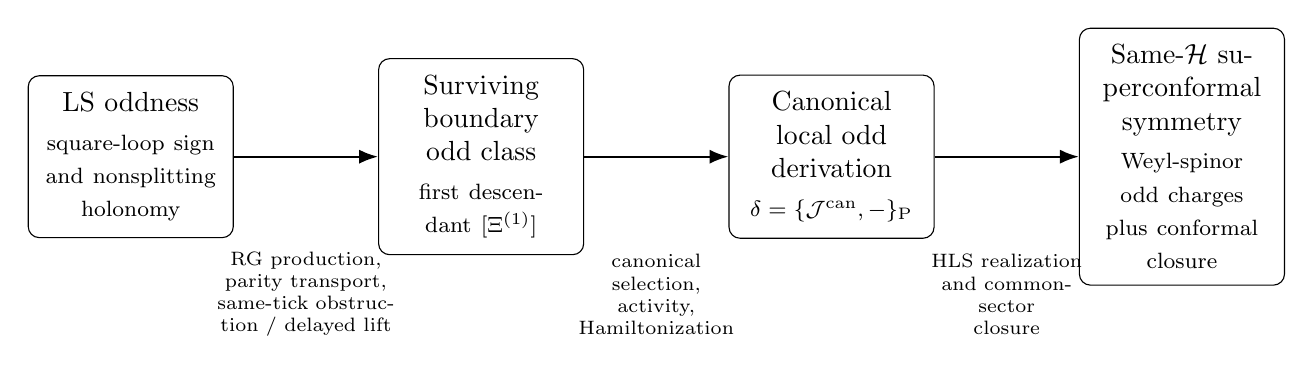
\begin{tikzpicture}[
  stage/.style={
    draw,
    rounded corners,
    align=center,
    text width=0.18\textwidth,
    minimum height=1.55cm,
    inner sep=6pt
  },
  flow/.style={-{Latex[length=2.4mm]}, thick},
  flowlabel/.style={font=\scriptsize, align=center, text width=0.19\textwidth}
]
\node[stage] (ls) at (0,0) {LS oddness\\[2pt]
  \footnotesize square-loop sign and nonsplitting holonomy};
\node[stage] (desc) at (4.45,0) {Surviving boundary odd class\\[2pt]
  \footnotesize first descendant \([\Xi^{(1)}]\)};
\node[stage] (delta) at (8.90,0) {Canonical local odd derivation\\[2pt]
  \footnotesize \(\delta=\{\mathcal J^{\mathrm{can}},-\}_{\mathrm P}\)};
\node[stage] (sym) at (13.35,0) {Same-\(\mathcal H\) superconformal symmetry\\[2pt]
  \footnotesize Weyl-spinor odd charges plus conformal closure};

\draw[flow] (ls) -- (desc);
\draw[flow] (desc) -- (delta);
\draw[flow] (delta) -- (sym);

\node[flowlabel] at ($(ls)!0.5!(desc)+(0,-1.75)$)
  {RG production,\\parity transport,\\same-tick obstruction / delayed lift};
\node[flowlabel] at ($(desc)!0.5!(delta)+(0,-1.75)$)
  {canonical selection,\\activity,\\Hamiltonization};
\node[flowlabel] at ($(delta)!0.5!(sym)+(0,-1.75)$)
  {HLS realization\\and common-sector\\closure};
\end{tikzpicture}
\caption{Introduction-level roadmap for the Main theorem.  The nodes indicate
what kind of odd object is available at each stage; the arrows indicate what
the theorem must still do in order to pass to the next stage.}
\label{fig:intro-roadmap}
\end{figure}

Here \([\Xi^{(1)}]\) denotes the odd first-descendant class produced by the RG
interface, \(\mathcal J^{\mathrm{can}}\) its derived canonical
representative, and \(\delta\) the resulting Hamiltonized odd derivation.  Only
this Hamiltonized derivation enters Haag--\L opusza\'nski--Sohnius.

The two bosonic times play fundamentally different roles.  Physical time
organizes real-time propagation, descent, and Ward identities.  RG time
organizes coarse-graining and produces the odd anomaly insertion that the
theorem tracks.  There is no general reason why these two times should yield
odd boundary symmetry.  The theorem isolates the required mechanism: RG time
must produce a genuine odd shadow, and that shadow must survive the relevant
reduction steps and remain active in the even sector.

The theorem excludes theories in which the odd shadow is absent, scheme-trivial, destroyed by the
relevant quotient, or present only as a dynamically dark sector.  This will be
unpacked later in Section~\ref{sec:rg-monotone-good}; for now the important
point is that the theorem identifies a bridge from the LS oddness to
superconformal symmetry, not a universal statement about every two-time model.

The base theorem stops at same-\(\mathcal H\) superconformal closure.  That
endpoint is already strong: the odd charges and conformal generators act on one
and the same UV Hilbert space and close to the full four-dimensional
superconformal algebra.  The stronger claim forcing \(\mathcal N=4\) belongs to
a separate optional criterion with additional assumptions.  It should not be
confused with the base realization theorem.

One further warning already matters at the level of orientation: ghost parity,
physical \(\Gamma\)-parity, and the LS holonomy character \(\omega\) must not be
identified.  Their precise roles are fixed in Section~\ref{sec:setup-body}
before the main statement is given.

Accordingly, the proposal does not assume an initial odd AQFT derivation, a
Hilbert-space odd implementer supplied at the start, Weyl-spinor generators or
superalgebra closure inserted by hand, an a priori superconformal multiplet, or
an identification of the physical-time BRST differential \(Q_t\) with a
microscopic supercharge.

The paper is organized as follows.  Section~\ref{sec:setup-body} formulates the
two-time boundary setting, lays out the relevant failure modes, organizes the
assumption packages by role, and states the main theorem.  Section~\ref{sec:cptp-brst}
then gives the transport chain itself, from the LS sign action to the
Hamiltonized odd derivation.  Section~\ref{sec:UV-fixed-point} separates the
base same-\(\mathcal H\) superconformal closure theorem from the stronger
optional maximality criterion.  Sections~\ref{sec:rg-monotone-good}
and~\ref{sec:discussion} are not afterthoughts: they explain what class of
theories the theorem actually selects, what the LS input contributes inside
that class, why the ledger question matters, and how a microscopic
realization is expected to fit into the broader program.

\section{Setting, assumptions, and main theorem}
\label{sec:setup-body}

We now formulate the theorem as a statement about a generic \(AdS_5\) UV
boundary equipped with two bosonic times.  The assumptions are presented in
package form because the theorem is not a one-step implication.  It begins with
the LS odd holonomy, passes through RG descendant formation and local
selection, and ends only after Hamiltonization and Hilbert-space symmetry
closure have been established.

\subsection{Two bosonic times and one local target}
\label{subsec:two-time-arrows}

We work with a five-dimensional \(AdS_5\) background whose conformal boundary
admits a four-dimensional Lorentzian local quantum field theory on a Minkowski
UV chart.  Physical time \(t\) and radial/RG time \(u\) are treated as two
independent monotonic directions.  Physical time acts through ordinary
Lorentzian evolution.  RG time acts through the radial/Wilsonian direction.
The Schwinger--Keldysh completion is assumed to make both time directions visible on the
same sufficiently local class of boundary observables, so that the analysis can
be carried out inside one local framework.  This common framework is not a
convenience.  If physical time and RG time lived only on different
descriptions, their odd descendants could fail to communicate and the theorem
would have no coherent local target.

Within this framework the SK construction supplies a two-time BRST bicomplex
\((Q_t,Q_u)\) on sufficiently local observables.  The operator \(Q_t\) belongs
to the real-time SK structure and organizes descent and Ward identities.  The
operator \(Q_u\) belongs to the RG direction and is the source of the odd
insertion that the theorem tracks.  The two differentials are therefore not
interchangeable.  The theorem follows the RG-produced odd descendant
\(Q_u^{\mathrm{phys}}\mathcal O^{(0)}\), not the physical-time differential
\(Q_t\) itself.

Next point must be kept sharp: the LS chain bicomplex and the boundary BRST
bicomplex are not identified.  The LS theorem supplies an odd holonomy and a
sign action; the Main theorem shows how that sign action reaches the local
boundary descendant quotient.  Only after parity transport, nonvanishing, and
canonical selection does one obtain the Hamiltonized odd derivation
\(
\delta=\{\mathcal J^{\mathrm{can}},-\}_{\mathrm P}
\)
that enters the Hilbert-space symmetry theorem.

\subsection{Failure modes and package architecture}
\label{subsec:failure-modes-main}

At this stage neither supersymmetry nor a local odd charge is assumed.  The
problem is instead to determine whether the two-time data force a genuine odd
boundary channel with physical content.  Four obstructions can prevent this
from happening:
\begin{enumerate}[label=\textnormal{(\roman*)},leftmargin=*,itemsep=0.25em]
  \item RG time may fail to produce a genuine odd first descendant once
  scheme contributions are removed;
  \item the LS sign action may fail to survive transport into the
  local descendant quotient;
  \item a surviving odd class may remain physically dark, acting trivially on
  all sufficiently local even probes;
  \item even a nontrivial active odd derivation may fail to satisfy the
  locality, covariance, energy, or implementability requirements needed for a
  Hilbert-space symmetry theorem and conformal closure.
\end{enumerate}
The package stack is organized exactly around these failure modes.  One part of
the stack supplies the LS holonomy input, a second part produces and stabilizes the local odd
descendant class, a third part promotes that class to a genuine derivation, and
a final part places the resulting derivation inside the Hilbert-space and
conformal framework where HLS and same-\(\mathcal H\) closure apply.

\subsection{Package synopsis and main statement}
\label{subsec:assumptions-main}

The assumption packages are best read in four gates rather than as one
undifferentiated bundle.
\begin{itemize}
  \item \textbf{LS oddness.}
  The package \(\mathbf{2T}_{\mathrm{LS}}\) supplies the parity cocycle, the
  nonsplitting \(\mathbb Z_2\)-cover, the detector-based distinguishability
  statement, and the square-loop sign action.  This is the oddness that
  the Main theorem attempts to realize on the boundary.

  \item \textbf{Descendant formation.}
  The package \(\mathbf{2T}_{\mathrm{RG}}\) provides an even sufficiently local
  representative \(\mathcal O^{(0)}\), decomposes the RG odd operator into
  physical and scheme parts, and isolates the genuine odd insertion
  \(Q_u^{\mathrm{phys}}\mathcal O^{(0)}\).  Together with
  \(\mathbf{2T}_{\mathrm{char}}^{\mathrm{weak}}\), it places the resulting odd
  data in the affine descendant class \([\Xi^{(1)}_{\Lambda_k}]\) where one can
  ask whether a genuine odd direction survives.

  \item \textbf{Survival and visibility.}
  The supplement \(\mathbf{2T}_{\mathrm{sel}}\) provides the same-tick
  obstruction lane on the abstract selected quotient, while
  \(\mathbf{2T}_{\mathrm{sel}}^{\mathrm{delay}}\) furnishes the delayed
  quotient-first route at the successor ledger step.  Together
  they keep the selected odd channel alive at the right abstract and physical
  interfaces.  The supplement
  \(\mathbf{2T}_{\mathrm{char}}^{\mathrm{act}}\) requires this selected odd
  direction to be visible to at least one sufficiently local even probe, so
  that the surviving odd channel is not physically dark.  The Peierls package
  \(\mathbf{2T}_{\mathrm{Peierls}}\) then converts the selected sufficiently
  local representative into a genuine derivation on observables.

  \item \textbf{Boundary symmetry closure.}
  The energy-bounds/covariance package \(\mathbf{2T}_{\mathrm{EBC}}\) supplies
  the UV locality, covariance, vacuum, and energy-control hypotheses needed for
  AQFT reconstruction and for the verification of the
  Haag--\L opusza\'nski--Sohnius interface.  The conformal common-sector package
  \(\mathbf{2T}_{\mathrm{conf}}\) ensures that the conformal generators and the
  odd charges act on one vacuum representation and one common invariant core,
  so that the odd symmetry sector closes with the \(SO(4,2)\) generators on a
  single Hilbert space.
\end{itemize}

Two structural remarks are crucial.  First,
\(\mathbf{2T}_{\mathrm{char}}^{\mathrm{cal}}\) is not a separate primitive
assumption.  It is derived from
\(\mathbf{2T}_{\mathrm{char}}^{\mathrm{weak}}\) and supplies the Hilbertizing
form used to select the canonical representative
\(\mathcal J^{\mathrm{can}}\).  Second, the BRST, AQFT, and HLS structures are
not independent axioms inserted by hand.  The SK construction supplies the BRST
bicomplex, the UV locality/covariance data supply the AQFT representation, and
the Hamiltonized odd derivation is then shown to satisfy the HLS hypotheses.
The odd derivation and the superconformal algebra are therefore derived
consequences of the package hypotheses.

\begin{remark}[Three \(\mathbb Z_2\) parities (do not mix)]
\label{rem:three-Z2-main}
We keep three distinct \(\mathbb Z_2\) parities throughout the analysis:
\emph{ghost parity} (SK/BRST cohomological degree mod \(2\)),
\emph{physical parity} \(\Gamma\) (an involutive \( * \)-automorphism on the
observable net, defining \(\Gamma\)-even and \(\Gamma\)-odd sectors), and the
\emph{Limited-Scope holonomy} \(\omega\in\mathbb Z_2\) of the procedure cover,
represented on observables by \(\Gamma^\omega\).  Ghost parity is bookkeeping,
whereas \(\Gamma\) and \(\omega\) are physical.  The LS chain bicomplex
\((Q_t^{\mathrm{ch}},Q_u^{\mathrm{ch}})\) and the boundary BRST bicomplex
\((Q_t,Q_u)\) are not identified; they interact only through the
parity-transport step described in Appendix~\ref{sec:parity-bridge}.
\end{remark}

\begin{theorem}[2T-Main theorem, informal]
\label{thm:main}
Consider a generic \(AdS_5\) setup whose UV boundary admits a four-dimensional
local quantum field theory together with the assumption packages
\[
\mathbf{2T}_{\mathrm{LS}}
\;+\;
\mathbf{2T}_{\mathrm{RG}}
\;+\;
\mathbf{2T}_{\mathrm{Peierls}}
\;+\;
\mathbf{2T}_{\mathrm{EBC}}
\;+\;
\mathbf{2T}_{\mathrm{char}}^{\mathrm{weak}}
\;+\;
\mathbf{2T}_{\mathrm{char}}^{\mathrm{act}}
\;+\;
\mathbf{2T}_{\mathrm{sel}}
\;+\;
\mathbf{2T}_{\mathrm{sel}}^{\mathrm{delay}}
\;+\;
\mathbf{2T}_{\mathrm{conf}},
\]
and suppose that the two-time Schwinger--Keldysh construction furnishes the
corresponding BRST bicomplex on sufficiently local observables.  Then the
following statements hold.
\begin{enumerate}[label=\textnormal{(\roman*)},leftmargin=*,itemsep=0.35em]
  \item The RG package produces a genuine odd first-descendant class
  \([\Xi^{(1)}_{\Lambda_k}]\), and the LS square-loop is transported by
  parity to a sign action on its selected quotient image
  \(\overline{\Xi}^{(1)}_{\Lambda_k}\).

  \item The same-tick selected-line supplement provides the obstruction route on
  that abstract quotient, while the delayed selected-line supplement supplies a
  nonzero quotient point at the successor ledger step.  Together
  they provide the nonvanishing input used by the derived calibration package
  to select a unique nonzero canonical odd representative
  \(\mathcal J^{\mathrm{can}}_{\Lambda_k}\in[\Xi^{(1)}_{\Lambda_k}]\).

  \item The activity supplement shows that this canonical odd line is not
  locally dark, and the Peierls bracket Hamiltonizes
  \(\mathcal J^{\mathrm{can}}_{\Lambda_k}\) into a nontrivial local
  \(\Gamma\)-odd derivation
  \[
  \delta_{\Lambda_k}
  =
  \{\mathcal J^{\mathrm{can}}_{\Lambda_k},-\}_{\mathrm P,\Lambda_k}.
  \]

  \item The AQFT and Haag--\L opusza\'nski--Sohnius hypotheses are satisfied by
  this Hamiltonized derivation.  Hence the UV boundary carries a
  finite-dimensional Weyl-spinor odd charge module on the same vacuum
  representation, with indexed generators \(Q_\alpha^I\) and
  \(\bar Q_{\dot\alpha I}\) satisfying
  \[
  \{Q_\alpha^I,\bar Q_{\dot\beta J}\}
  =
  2\,\delta^I{}_J\,\sigma^\mu_{\alpha\dot\beta}P_\mu,
  \qquad
  \{Q_\alpha^I,Q_\beta^J\}
  =
  \{\bar Q_{\dot\alpha I},\bar Q_{\dot\beta J}\}=0;
  \]

  \item Combining the odd charge module with the common conformal sector yields
  the full four-dimensional superconformal algebra on the same Hilbert space.
  More precisely, the resulting operator Lie superalgebra is
  \(\mathfrak{su}(2,2|N)\) for \(N\neq4\), while in the \(N=4\) case the
  standard simple form is obtained after quotienting the central
  \(\mathfrak u(1)\), giving \(\mathfrak{psu}(2,2|4)\).
\end{enumerate}
\end{theorem}

The base conclusion of the theorem is therefore same-\(\mathcal H\)
superconformal closure.  The odd sector is not inserted by hand.  It is
reconstructed from the RG descendant, stabilized by the same-tick obstruction
and delayed selected-line supplements, made dynamically meaningful by activity
and Hamiltonization, and only then promoted to Hilbert-space symmetry by HLS.

This is the natural endpoint of the base realization theorem.  Forcing
\(N=4\) is a separate strengthening problem.  It uses additional structural
assumptions on the UV fixed point and should not be folded back into the
assumption burden of the base theorem.

\begin{proposition}[Strengthened maximality criterion]
\label{prop:main-optional-4c}
Assume, in addition to the hypotheses of Theorem~\ref{thm:main}, that the UV
fixed point is non-gravitational with a unique stress tensor, genuinely
interacting in the sense that the SK RG monotone has a nondegenerate UV
extremum and no decoupled free SCFT sector is present, and carries no
higher-spin enhancement.  Assume also the standard spin-2 saturation input
that a unitary four-dimensional superconformal theory with \(N>4\) and a
unique stress tensor must contain a graviton and therefore cannot occur in the
non-gravitational setting, and assume that interacting non-gravitational
SCFTs exist for each \(N\in\{1,2,3,4\}\).

Finally impose the following \emph{maximality principle}: among
SK-admissible UV fixed points compatible with the same macroscopic data
(dimension, locality, spin range, and the standing two-time structure), the
RG dynamics selects those with the largest available unbroken symmetry.  In
particular, once the allowed superconformal algebras have been reduced to
\(\mathfrak{su}(2,2|N)\) with \(1\le N\le4\), the realized fixed point takes
the largest admissible \(N\); a smaller value of \(N\) cannot be compensated
by adding further continuous symmetries without changing the universality
class.

Then the superconformal multiplicity parameter is forced to be \(N=4\).  This
yields a separate optional criterion for maximal \(\mathcal N=4\)
supersymmetry, as summarized in Proposition~\ref{prop:4c-N-equals-4}.
\end{proposition}

Section~\ref{sec:cptp-brst} now proves the transport-and-realization chain
announced above.  Section~\ref{sec:UV-fixed-point} establishes the exact closure
endpoint and keeps it separate from maximality.  Only after that theorem spine
is in place do Sections~\ref{sec:rg-monotone-good} and~\ref{sec:discussion}
return to the broader interpretive questions: what class of theories is really
being selected, what the LS input contributes inside that class, and what a
concrete ledger realization would have to supply.

\section{From LS holonomy to a boundary odd derivation}
\label{sec:cptp-brst}

The core logic of the theorem is best read as a transport-and-realization
chain.  The LS theorem gives an odd sign action.  The Main theorem shows how
that sign action reaches the selected descendant quotient, forces nonvanishing,
produces a canonical odd representative, and finally becomes a local odd
derivation with symmetry consequences.  Each step removes a distinct
obstruction.

\begin{enumerate}[label=\textnormal{(\arabic*)},leftmargin=*,itemsep=0.55em]
  \item \textbf{LS parity transport.}  The Limited Scope theorem
  provides the square-loop sign action at the record/process level.  This is
  only the beginning.  The Main theorem still has to transport that sign action
  to the boundary descendant sector.  The parity-transport step identifies the
  LS square-loop action with physical parity on first descendants, but this
  transport is meaningful only after one specifies the selected local quotient
  in which the boundary odd channel is to live.

  \item \textbf{RG time produces the odd descendant class.}  The package
  \(\mathbf{2T}_{\mathrm{RG}}\) provides an even sufficiently local
  representative \(\mathcal O^{(0)}\), decomposes the RG odd operator into
  physical and scheme parts, and isolates the genuine odd insertion
  \(Q_u^{\mathrm{phys}}\mathcal O^{(0)}\).  The anomalous descent relation
  \[
  Q_u^{\mathrm{phys}}\mathcal O^{(0)}+Q_t\Xi^{(1)}=\mathcal A^{(1)}
  \]
  is the first place where bosonic RG time produces the odd class
  \([\Xi^{(1)}_{\Lambda_k}]\) used by the theorem.  This is why the theorem
  follows the RG anomaly sector rather than treating \(Q_t\) as the symmetry
  generator.

  \item \textbf{The same-tick obstruction package realizes the LS sign action on
  the abstract selected quotient.}  The supplement
  \(\mathbf{2T}_{\mathrm{sel}}\) isolates a nonzero odd line in the descendant
  ambiguity group and provides the obstruction contract required to transport
  the LS sign action to the selected quotient image
  \(\overline{\Xi}^{(1)}_{\Lambda_k}\).  This is the precise abstract
  bridge from the LS holonomy landscape to the Main descendant quotient.

  \item \textbf{The delayed selected-line package gives the delayed-step
  nonvanishing route.}  The supplement
  \(\mathbf{2T}_{\mathrm{sel}}^{\mathrm{delay}}\) furnishes a nonzero
  quotient point at the successor step together with the
  delayed split-to-descendant map and the separate dominant-response gate.
  This is the physically relevant odd-to-even export interface.  With the
  same-tick obstruction route and the delayed route both present, the odd class
  cannot collapse away before canonicalization.

  \item \textbf{The nonzero class yields a canonical odd representative and a
  local odd derivation.}  The derived calibration supplement supplies the
  Hilbertizing form needed to choose the unique norm-minimizing representative
  \(\mathcal J^{\mathrm{can}}_{\Lambda_k}\in[\Xi^{(1)}_{\Lambda_k}]\).  The
  activity supplement then guarantees that this distinguished odd direction is
  not locally dark.  The Peierls package Hamiltonizes it to
  \[
  \delta_{\Lambda_k}
  =
  \{\mathcal J^{\mathrm{can}}_{\Lambda_k},-\}_{\mathrm P,\Lambda_k}.
  \]
  This is the point at which the odd content stops being a quotient class and
  becomes a local odd derivation on observables.

  \item \textbf{HLS promotes the Hamiltonized derivation to a Weyl-spinor odd
  charge module.}  The energy-bounds/covariance package, together with the UV
  locality data, places the theory in the setting where AQFT reconstruction and
  Haag--\L opusza\'nski--Sohnius apply.  HLS does not act on \(Q_t\); it acts on
  the Hamiltonized derivation \(\delta\).  The conclusion is a
  finite-dimensional Weyl-spinor odd charge module with indexed generators
  \(Q_\alpha^I\) and \(\bar Q_{\dot\alpha I}\).

  \item \textbf{The odd charge module closes with the conformal sector on the
  same Hilbert space.}  The conformal common-sector package ensures that the
  conformal generators and the odd charges act on one vacuum representation and
  one common invariant core.  The result is same-\(\mathcal H\)
  superconformal closure.  Only after this base closure theorem is in place
  does it make sense to ask whether stronger assumptions force \(N=4\).
\end{enumerate}

Two remarks summarize the mechanism.  First, the theorem’s central generator is
not \(Q_t\) but \(\delta\).  The role of \(Q_t\) is to organize descent and Ward
identities.  Second, the same-tick obstruction supplement, the delayed
selected-line supplement, and the activity supplement solve different problems.
The first gives the abstract no-extra-collapse route, the second gives the
quotient route through the successor ledger step, and the third prevents the surviving odd
channel from remaining physically dark.  The logic is therefore rigid:
removing any one of these steps breaks a different part of the chain.

\section{Superconformal closure versus maximality}
\label{sec:UV-fixed-point}

The intrinsic endpoint of the base theorem is same-\(\mathcal H\)
superconformal closure.  This means that the conformal generators inherited
from the \(AdS_5\) boundary geometry and the odd generators obtained from the
Hamiltonized descendant sector act on one and the same UV Hilbert space.  The
result is already strong: it is not merely the existence of an odd charge
module, but the closure of that module with the full four-dimensional
conformal algebra.

At this stage the theorem yields the precise distinction
\[
\mathfrak{su}(2,2|N)\quad (N\neq4),
\qquad
\mathfrak{psu}(2,2|4)\quad (N=4).
\]
For \(N=4\) the simple superalgebra is obtained only after quotienting the
central \(\mathfrak u(1)\), which is why the natural final form is
\(\mathfrak{psu}(2,2|4)\).

This closure theorem is already substantial even before any maximality claim
is made.  It says that the odd channel reconstructed from the RG descendant is
not an isolated algebraic artifact; it integrates coherently with the full
four-dimensional conformal symmetry on the physical UV Hilbert space.

It is mathematically essential to separate this closure theorem from the
stronger criterion forcing \(N=4\).  The stronger criterion uses additional
assumptions: non-gravitationality, spin-2 saturation, interaction, absence of
higher-spin enhancement, and the existence and maximality conditions recorded
in the strengthening analysis.  These assumptions restrict the UV fixed point in ways that go beyond the
odd-channel realization problem itself.

For this reason the theorem naturally has two layers of conclusion.
\begin{enumerate}[label=\textnormal{(\roman*)},leftmargin=*,itemsep=0.35em]
  \item The base theorem yields same-\(\mathcal H\) superconformal closure and
  determines the superconformal algebra up to the multiplicity parameter
  \(N\).
  \item The strengthened maximality criterion imposes additional structural
  assumptions and then forces \(N=4\).
\end{enumerate}

These layers provide clear distinction in assumption burden so the logical structure of the result is transparent.

\section{Physical meaning and scope}
\label{sec:rg-monotone-good}

\subsection{What class of theories is selected?}

These assumptions do not single out
``supersymmetric theories'' in any direct or circular way.  What they single
out is a narrower and more precise class: theories in which the bosonic
two-time structure supports a nontrivial odd shadow that survives all
reduction steps and remains physically active on the UV boundary.  The
restrictive assumptions are therefore concentrated in three places: the RG
package, the selected-line supplement, and the activity supplement.

\begin{enumerate}[label=\textnormal{(\arabic*)},leftmargin=*,itemsep=0.4em]
  \item \textbf{The theorem excludes a purely bosonic RG sector.}  If the RG
  monotone can be
  described, after removing scheme terms, without a genuine odd insertion
  \(Q_u^{\mathrm{phys}}\mathcal O^{(0)}\), then the theory lies outside the
  admissible class.  The point is not that every bosonic theory is ruled out,
  but that the class treated here must have an odd cohomological shadow
  attached to its RG time.

  \item \textbf{The theorem excludes a scheme-trivial odd shadow.}  If the odd
  RG insertion is
  killed by \(Q_t\)-exactness or can be absorbed entirely into scheme
  redefinitions, then the odd channel carries no invariant physical content and
  the theorem does not apply.  Thus the odd descendant must encode more than a
  bookkeeping artifact of the renormalization scheme.

  \item \textbf{The theorem excludes collapse before the local descendant
  quotient.}  If a candidate odd line
  exists only in a coarser raw packet but dies when one passes to the
  descendant quotient, then the relevant selected-line package fails: either
  the same-tick obstruction route \(\mathbf{2T}_{\mathrm{sel}}\) is not
  available on the abstract selected carrier, or the delayed route
  \(\mathbf{2T}_{\mathrm{sel}}^{\mathrm{delay}}\) does not produce the
  quotient point at the successor ledger step.  The theorem therefore requires not just
  abstract odd data, but odd data that survives the precise quotient procedure
  relevant to the local boundary theory.

  \item \textbf{The theorem excludes a physically dark odd sector.}  If the
  selected odd line
  survives abstractly but acts trivially on every even sufficiently local
  probe, then \(\mathbf{2T}_{\mathrm{char}}^{\mathrm{act}}\) fails and the
  theory is excluded.  This is a minimal nondegeneracy requirement: the odd
  direction must be dynamically visible somewhere in the local even sector.
\end{enumerate}

The physical slogan is therefore the following.  The theorem applies to
theories in which bosonic RG time produces a genuine odd descendant, one
selected odd component survives the ambiguity and collapse steps, and that
surviving component is detectable through local even observables.  This is a
considerable restriction, but it is still weaker than assuming a fermionic symmetry
from the outset.

The selected class may therefore be described as proto-fermionic rather than
supersymmetric in the usual input sense.  These theories are distinguished not
because they begin with a supercharge, but because their two-time structure is
rich enough to support an odd sector that remains stable under all the
physically relevant reductions and can no longer be ignored dynamically.

\subsection{What does the LS input do inside the selected class?}

Entering the admissible class, the LS input supplies the physical picture of two times in our paradigm.  It introduces a \emph{classical ledger of
records}, a reversible microscopic time evolution between ledger checkpoints,
and an \emph{RG/coarse-graining operation that forgets fine-grained information} returning the world to the ledger point.  These two times are
ledger-mediated: one carries microscopic evolution between checkpoint, while the other changes how much of that evolution survives in the
recorded history.

LS then isolates the key fact about the interaction of these two times.  A
ledger by itself is not enough: if everything microscopic were already fixed by
the visible record, then ``live, then forget'' and ``forget, then live'' would
be the same story in two notations.  But the two-time square to be genuinely
nontrivial; it means there must be a \emph{completion sector} beyond the ledger, carrying
microscopic information that is not recorded at the checkpoint.

On the ledger itself, the square still closes: the same endpoint record can be
reached either way.  But one must also specify how the unrecorded microscopic
completion data are attached to that common corner.  That completion rule is
what LS calls a \emph{filler}.  LS singles out two canonical fillers, and their
difference is exactly the physical point: they agree on the same visible ledger
step, so they must be invisible there, yet they are not the same microscopic
realization.  Their mismatch survives in the completion sector as an
irreducible \(\mathbb Z_2\) sign.  That sign is objective.  It is not a matter
of notation, state relabeling, or endpoint bookkeeping.

LS does not select the theory class. Instead, it provides the underlying source of oddness: a genuine mismatch
between two filler-related microscopic completions of one and the same visible
ledger history.  Main then asks for the narrower class in which this hidden
completion-sector difference survives the reduction chain and reaches the UV
boundary as an active odd channel.

\subsection{But what is the ledger?}
\label{subsec:what-is-ledger}
The ledger is not the full microscopic state.  It is the accepted classical
record sector: the commuting facts that survive coarse-graining and define what
counts as the same visible history at a checkpoint.  Abstractly, what these records are made of can be ignored.  We use only the
structural claim that such a classical record layer exists and is rich enough so the Universe can perform RG/CPTP coarse-graining step, and that the completion sector carries the microscopic data that the ledger forgets.

These abstract claim level have considerable implications from 2T-LS and 2T-Main. 
\begin{itemize}
\item Wheeler's slogan ``it from bit'' becomes theorem-level statement~\cite{Wheeler1990ItFromBit};
\item $\mathbb{Z}_2$-gradedness surfaces in two deeply linked appearances:
\begin{itemize}
  \item objective distinction between before and after \emph{compatible with unitary evolution}; hence the real arrow of time that circumvents the hard wall of the constant von Neumann entropy.
  \item \emph{spinor symmetry} originating at the UV boundary; hence existence of the matter-rich Universe.
\end{itemize}
\item confluence of two appearances at a conformal boundary, conjecturally producing IIb microscopic theory in the standard $AdS_5/CFT_4$ setup.
\end{itemize}

This is why the ledger question matters so much.  If nature really contains
such a classical record layer, then the same structure would underwrite the whole chain from highest-level principle to microscopic theory.  

The present article stops one step short of identifying the ledger concretely.  That is a cosmology theory
question, and it is deferred to the discussion.

\section{Discussion}
\label{sec:discussion}

\subsection{Toward a cosmology realization}

A concrete answer to the ledger question requires a source theory that identifies, in one microscopic
construction, the record sector, the forgetting/coarse-graining operation, and the
completion data whose mismatch carries the LS sign.  

One proposed theory constructs ledger as a Weyl anomaly floor sector of a pure vacuum Karch-Randall \(AdS_4\) brane, which acts as a receiver that accumulates Brown-York flux from the incoming zero-area repeating pulses so that brane is physically holographically renormalized to a higher cutoff, moving in radial direction. 
\footnote{The governing principle is the least SK influence action that is uniquely minimized with the information export pulses of the temporally/spatially LoG/LoG shapes and receiver cutoff-bandlocked widths.}

The remaining anomaly floor is (a) classical, in the sense of being a local function on the brane and not an interacting field, and (b) preserves already stored facts due to widths band-locking. \footnote{Notably, \(AdS_5\) with three spatial dimensions is the minimal space which can contain a ledger of this type: even-\(d\) spaces does not contain a Weyl anomaly, while \(AdS_3\) anomaly floor is not a proper physical information storage, but rather a gauge/bookkeeping direction, and it explains how dimension-independent \(\mathbb{Z}_2\)-gradedness is realized in spinor symmetry only at \(d \ge 3\).}
A Fisher-odd direction feeds complementary sector that carries the odd completion residue not visible in the current
reduced receiver. Such a split af action into receiver wall-move, anomaly floor influx, and completion sector update makes two latter targets independent: the two filler-related
realizations in the completion sector remain indistinguishable in the receiver anomaly floor imprint. 

However, unlike the ledger, the completion sector influx is affine and bears increasing cost, so eventually the real wall-moving solution ceases to exist and completion/receiver complex splits.
In this split, that completion sector becomes the newborn source \(dS_4\) brane. \footnote{\emph{Source} here means that the oddness of completion sector surfaces as a brane coherence stock created by the split that feeds the next receiver due to QND-type leaks to the \(dS_4\) canonical commutant, which is geometrically situated between source and receiver branes along with the new completion sector.}

This sequence is CCC-like: the chain of \(dS_4\) observable Universes with an approximately conformal inheritance. Its ledger step is \emph{aeon}: the period from pre-split to pre-split finals of Universes, when the source coherences is maximally exhausted. So the accumulated \(\mathbb{Z}_2\) difference is eventually read and appears in the
ledger, but on the \emph{next step}.  This is the \emph{delayed zig-zag} picture: invisible on the current ledger, carried
through the completion sector, and first readable at the next receiver. Such a picture can be understood as a rough mirror of the 2T-LS ledger requirement: it provides the concrete physical mechanism by which two times mix and create the true holonomy over history.

Readers who want the full implementation package, including the 2T-LS and 2T-Main interface implementations,
exact audit reports, and 2T-LS formal proof in Agda, should consult the
archival workspace release~\cite{TwoTimesWorkspace2026}.

\subsection{Outlook}

In the light of 2T-Main results, several directions are proposed.  
\begin{enumerate}
  \item Obvious direction is strenghtning of the optional $\mathcal{N}=4$ step. It is expected that one could be resolved on the level of an implementation theory, hence search for such a theory can solidify the vertical chain proposed in Section \ref{subsec:what-is-ledger}.
  \item Another direction is strengthening of Main proof strategy. Currently, the post-Haag--\L opusza\'nski--Sohnius same-\(\mathcal H\) conformal closure step is existential only. Envisioned post-HLS transfer theorem could show that the package \(Q,\bar Q,S,\bar S\) itself is induced from the reduced data of implemention theory+2T-Main.
  \item Finaly, and this direction could be partially following from the first one, the post-HLS rigidity theorem could show that after transfer there is no hidden modulus beyond the candidate sign involution.
\end{enumerate}

If such a program is finished, we could state that the microscopic-level Universe is \(\mathbb{Z}_2\)-lift of its own history, accepted to the ledger.

The main conclusion, however, is already clear.  In the presence of the
assumption packages described above, two bosonic times can do more than generate an abstract odd holonomy.  They can force that oddness into a
surviving, locally effective boundary channel, and that channel can be
promoted to a superconformal symmetry algebra on the UV Hilbert space.

That is the sense in which the result should be read.  It is not a universal
statement about every theory with two times, and it is not a
hidden assumption of supersymmetry in alternative language.  It is a
structural theorem identifying a precise bridge from bosonic two-time data to
odd boundary symmetry.  Once that bridge exists, the symmetry consequences are
far more rigid than the microscopic starting point would have suggested.

\appendix
\IfFileExists{appendix_main.tex}{%
  % Proof appendix

\section{Guide to the logic}
\label{sec:appendix-guide}
This appendix isolates the minimal interfaces and implications needed to reach the
HLS classification step from the standing interface packages.  The guide below
follows the proof dependence rather than the raw appendix order: preparatory
subprograms are listed where they first enter the argument.
\begin{enumerate}[label=\textnormal{(\roman*)},leftmargin=*,itemsep=0.4em]
\item \textbf{Standing package bundle.} The standing assumptions are packaged as
  \(\mathbf{2T}_{\mathrm{Main}}\)
  \textnormal{(Definition~\ref{def:2T-Main})}, namely
  \[
  \mathbf{2T}_{\mathrm{LS}}
  + \mathbf{2T}_{\mathrm{RG}}
  + \mathbf{2T}_{\mathrm{Peierls}}
  + \mathbf{2T}_{\mathrm{EBC}}
  + \mathbf{2T}_{\mathrm{char}}^{\mathrm{cal}}
  + \mathbf{2T}_{\mathrm{char}}^{\mathrm{act}}
  + \mathbf{2T}_{\mathrm{sel}}
  + \mathbf{2T}_{\mathrm{sel}}^{\mathrm{delay}}
  + \mathbf{2T}_{\mathrm{conf}}.
  \]
  The record interface \(\mathbf{2T}_{\mathrm{rec}}\) and detector interface
  \(\mathbf{2T}_{\mathrm{det}}\) enter only through the LS summand, while the
  derived BRST package will be added below to form
  \(\mathbf{2T}_{\mathrm{Main}}^{\mathrm{spine}}\).
\item \textbf{Subprogram~1a (derived BRST).} Starting from the Lorentzian SK path
  integral, Subprogram~1a constructs the two-time BRST/bicomplex differentials
  \(Q_t,Q_u\) and their Ward identities on SK--admissible states, thereby
  producing the interface \(\mathbf{2T}_{\mathrm{BRST}}\) on the sufficiently
  local class \(\Fsloc\).  At that point the appendix spine works with
  \[
  \mathbf{2T}_{\mathrm{Main}}^{\mathrm{spine}}
  :=
  \mathbf{2T}_{\mathrm{Main}}+\mathbf{2T}_{\mathrm{BRST}}.
  \]
\item \textbf{Subprogram~2a (Results from the 2T Limited Scope Theorem).}  We import the LS
  parity cocycle, the nonsplitting \(\mathbb Z_2\)-cover, the detector witness,
  and the record-process-chain bicomplex identities.  This isolates the
  abstract two-time obstruction data that later feed the parity-transport step.
\item \textbf{Subprogram~2b (Cosmology theory Peierls bracket and swap invariance).}  We record
  the abstract Peierls package on sufficiently local boundary observables, its
  swap-equivariant Green operators, and the resulting Poisson automorphism
  property of the boundary swap involution.
\item \textbf{Subprogram~2c (Parity transport and physical \(\mathbb Z_2\) grading).}  Combining
  the LS import with the swap-equivariant boundary structures, we identify the
  physical parity involution \(\Gamma\) on first descendants and transport the
  LS square-loop sign to the boundary ambiguity sector.
\item \textbf{Subprogram~3a (selected-line nonvanishing, canonicalization, and characteristic activity).}
  This subsection packages the finite-cutoff canonical odd representative
  together with the same-tick obstruction lane, the delayed selected-line lane,
  the resulting nonvanishing statements, and the characteristic-algebra/activity
  consequences that follow once the odd descendant class survives.
\item \textbf{Subprogram~3b (RG monotone and Hamiltonized odd derivation).}
  The RG package \(\mathbf{2T}_{\mathrm{RG}}\) supplies the monotone and its
  anomalous descent source, while the Peierls and characterization packages are
  used to Hamiltonize the canonical odd representative and establish the local
  physically odd derivation \(\delta_{\Lambda_k}\).
\item \textbf{Subprogram~1b (local net, GNS reconstruction, and implementation template).}
  Subprogram~1b supplies the vacuum Wightman/AQFT representation
  \((\mathcal H,\pi,U,\Omega)\), the net \(O\mapsto\mathfrak A(O)\), and the
  dense implementation core on the Minkowski boundary.  These Hilbert-space
  inputs first enter when the argument passes from the local odd derivation to
  the AQFT/HLS step.
\item \textbf{Subprogram~3c (AQFT net and HLS on the Minkowski boundary).}
  Using \(\mathbf{2T}_{\mathrm{EBC}}\) together with the Subprogram~1b vacuum
  representation, Subprogram~3c extends \(\delta\) to the polynomial core,
  proves implementability of the odd derivation, verifies the HLS interface
  \(\mathbf{2T}_{\mathrm{HLS}}\), and identifies the finite-dimensional
  Weyl-spinor odd charge module on the UV vacuum representation.
\item \textbf{Subprogram~4a (dilatation weight \(\tfrac12\) of the odd charges on the common UV sector).}
  Combining the HLS odd module from Subprogram~3c, the HLS completeness
  statement, and the conformal common-sector package
  \(\mathbf{2T}_{\mathrm{conf}}\), Subprogram~4a places the odd charges on the
  common UV sector and forces their dilatation weight to be \(\tfrac12\).
\item \textbf{Subprogram~4b (same-\(\mathcal H\) conformal closure of the HLS odd sector).}
  With the weight-\(\tfrac12\) normalization from Subprogram~4a in hand,
  Subprogram~4b takes the finite conformal closure of the HLS odd seed,
  proves same-\(\mathcal H\) implementability of that odd conformal closure,
  recovers the degree-zero internal algebra, and identifies the resulting
  operator superalgebra with the standard \(4\)D superconformal algebra.
\item \textbf{Subprogram~4c (optional maximality strengthening).}
  This final section is not part of the base Main theorem.  It imports the
  superconformal closure from Subprogram~4b and studies what additional
  assumptions would force maximal supersymmetry, i.e.\ the optional
  \(N=4\) conclusion at the UV fixed point.
\end{enumerate}

\section{Master packages and interface assumptions}
\label{sec:setup}

\subsection{Master package block}

\subsubsection{Input Interfaces}

\begin{definition}[Record two--time interface $\mathbf{2T}_{\mathrm{rec}}$]
\label{def:2T-rec}
A \emph{record two--time interface} consists of:
\begin{enumerate}[label=\textbf{(R\arabic*)},leftmargin=*,itemsep=0.5em]
\item \textbf{SK and records.} Sets $\SKstates$ (SK states) and $\Sys$ (record states),
  a map $\diag:\Sys\to\SKstates$, and an involution $\swap:\SKstates\to\SKstates$ such that
  $\swap^2=\mathrm{id}_{\SKstates}$ and $\swap\circ\diag=\diag$.
\item \textbf{Two arrows.} A group $T$ and the additive monoid $(\mathbb R_{\ge 0},+,0)$,
  with actions $\mathrm{act}_T:T\times\SKstates\to\SKstates$ and
  $\mathrm{act}_U:\mathbb R_{\ge 0}\times\SKstates\to\SKstates$
  satisfying the action axioms and \emph{weak commutativity} on $\SKstates$:
  \[
  \mathrm{act}_U(u,\mathrm{act}_T(t,x))=\mathrm{act}_T(t,\mathrm{act}_U(u,x)).
  \]
\item \textbf{Strict RG diagonalization.} For each $u>0$ a map
  $\Pi_u:\SKstates\to\Sys$ and a record RG action $R_u:\Sys\to\Sys$ such that
  \[
  \mathrm{act}_U(u,x)=\diag(\Pi_u(x)),\qquad
  \Pi_u(\diag r)=R_u(r)\quad(u>0),
  \]
  with $R_0=\mathrm{id}$ and $R_{u_2+u_1}=R_{u_2}\circ R_{u_1}$.
\item \textbf{Chosen RG sector (reachability).} A section
  $\mathrm{sec}_\Pi:\Sys\to\SKstates$ with $\Pi_1(\mathrm{sec}_\Pi(r))=r$.
\item \textbf{No mixed anomaly at the boundary of squares.}
  A bisimplicial set $\mathcal C^{\mathrm{SK}}_{m,n}$ with horizontal and vertical face maps
  $d_i^H,d_j^V$ satisfying simplicial relations in each direction and mixed
  commutation $d_i^H d_j^V=d_j^V d_i^H$~\cite{GoerssJardine1999Simplicial}.
\item \textbf{Record reflection.} Diagonal cancellation:
  \[
  \diag(r)=\diag(r') \Rightarrow r=r'.
  \]
\end{enumerate}
\end{definition}

\begin{remark}
The discrete RG-step case is recovered by restricting $u\in\mathbb N\subset\mathbb R_{\ge 0}$.
\end{remark}

\begin{definition}[Detector interface $\mathbf{2T}_{\mathrm{det}}$]
\label{def:2T-det}
A \emph{detector interface} is any additional structure that implies the
$\mathbb Z_2$--action on the difference object $\Diff=\mathrm{Cofib}(\diag)$ is
nontrivial, i.e.\ $\flip\neq \mathrm{id}_{\Diff}$ or equivalently there exists
$y\in\Diff$ with $\flip(y)\neq y$.
\end{definition}

\begin{definition}[Limited Scope package $\mathbf{2T}_{\mathrm{LS}}$]
\label{def:2T-LS}
Define the \emph{2T Limited Scope package} by
\[
\mathbf{2T}_{\mathrm{LS}} := \mathbf{2T}_{\mathrm{rec}} + \mathbf{2T}_{\mathrm{det}}.
\]
\end{definition}

\begin{definition}[Two independent $\mathbb Z_2$ gradings]
\label{def:two-gradings}
We distinguish:
\begin{enumerate}[label=\textnormal{(\alph*)},leftmargin=*,itemsep=0.2em]
\item \emph{Cohomological/BRST parity} $|\cdot|_{\mathrm{ch}}\in\mathbb Z_2$ on the
  cochain algebra $\Fsloc=(\Fsloc)_{\bar 0}\oplus(\Fsloc)_{\bar 1}$, with
  $|Q_t|_{\mathrm{ch}}=|Q_u|_{\mathrm{ch}}=1$.
  Accordingly, $H^0(\Fsloc,Q_t)$ and $H^1(\Fsloc,Q_t)$ denote even/odd cohomology.
\item \emph{Physical parity} $|\cdot|_{\Gamma}\in\mathbb Z_2$ induced by the involution
  $\Gamma$ (SK swap), giving a decomposition into $\Gamma$--even/odd parts
  $\Fsloc={\Fsloc}^{+}\oplus{\Fsloc}^{-}$.
\end{enumerate}
Oddness in the AQFT/HLS steps always refers to $|\cdot|_{\Gamma}$.
\end{definition}

\begin{definition}[RG--monotone interface $\mathbf{2T}_{\mathrm{RG}}$]
\label{def:2T-RG}
An \emph{RG--monotone interface} consists of:
\begin{enumerate}[label=\textbf{(M\arabic*)},leftmargin=*,itemsep=0.5em]
\item \textbf{Monotone and representative.} A real monotone $M(u)$ near the UV
  ceiling $u_0$, a family of SK--admissible states $\rho_u$, and a quasi--local
  family $\mathcal O^{(0)}(u)\in\Fsloc$ with
  \[
  M(u)=\langle \mathcal O^{(0)}(u)\rangle_{\rho_u},
  \qquad
  Q_t\mathcal O^{(0)}(u)=0,
  \qquad
  [\mathcal O^{(0)}(u_0)]\neq 0\in H^0(\Fsloc,Q_t).
  \]
\item \textbf{RG Ward identity (odd form, refined).} On the monotone representative
  $\mathcal O^{(0)}(u)$, decompose the $u$--differential as
  \[
  Q_u = Q_u^{\mathrm{phys}} + Q_u^{\mathrm{scheme}},
  \]
  where $Q_u^{\mathrm{scheme}}$ encodes scheme/reparametrisation effects
  (local counterterm and coupling redefinition ambiguities). We assume that
  $Q_u^{\mathrm{phys}}$ and $Q_u^{\mathrm{scheme}}$ are odd derivations
  on $\Fsloc$.
  We additionally assume $Q_u^{\mathrm{phys}}$ and $Q_u^{\mathrm{scheme}}$ are
  \emph{presheaf derivations}: for every double cone $O$ they restrict to odd
  derivations
  \[
  Q_u^{\mathrm{phys}}:\Fsloc(O)\to\Fsloc(O),\qquad
  Q_u^{\mathrm{scheme}}:\Fsloc(O)\to\Fsloc(O).
  \]
  Finally, we assume they anticommute with $Q_t$ on this class (so
  $Q_u^{\mathrm{phys}}\mathcal O^{(0)}$ is $Q_t$--closed whenever
  $Q_t\mathcal O^{(0)}=0$), and that for $u$ near $u_0$,
  \[
  \frac{d}{du}M(u)
  = -\big\langle (Q_u^{\mathrm{phys}}\mathcal O^{(0)})(u)\big\rangle_{\rho_u},
  \qquad
  \big\langle (Q_u^{\mathrm{scheme}}\mathcal O^{(0)})(u)\big\rangle_{\rho_u}=0,
  \]
  up to expectation values of $Q_t$--exact terms (which vanish for
  SK--admissible states by $\mathbf{2T}_{\mathrm{BRST}}$-\textbf{(B2)}).
\par
  \textbf{Cohomological triviality of scheme terms on the monotone sector.}
  For every $X\in{\Fsloc}_{\mathrm{mon}}$ with $Q_tX=0$, we assume
  \[
  [\,Q_u^{\mathrm{scheme}}X\,]=0\quad\text{in}\quad H^1(\Fsloc,Q_t).
  \]
\par
  (Optional packaging.) Equivalently, one may encode the same information by an
  even derivation $L_{\rm RG}$ on $\Fsloc$ (Callan--Symanzik plus anomaly/contact
  terms) with
  $
  \tfrac{d}{du}M(u)=\langle (L_{\rm RG}\mathcal O^{(0)})(u)\rangle_{\rho_u}.
  $
\item \textbf{Anomalous first descent (no Ward trivialization).}
  There exist sufficiently local raw first-descendant potentials
  \(\Xi^{(1)}(u)\in\Fsloc\)
  and an anomaly insertion $\mathcal A^{(1)}(u)\in(\Fsloc)_{\bar 1}$ such that
  \begin{equation}
  \label{eq:anom-descent}
  Q_u^{\mathrm{phys}}\mathcal O^{(0)}(u)\ +\ Q_t\Xi^{(1)}(u)\ =\ \mathcal A^{(1)}(u),
  \qquad
  Q_t\mathcal A^{(1)}(u)=0.
  \end{equation}
  We interpret \eqref{eq:anom-descent} as an identity in the locality quotient
  (Definition~\ref{def:locality-quotient}); in particular, $\mathcal A^{(1)}(u)$
  represents the $Q_t$--cohomology class
  $\big[\,Q_u^{\mathrm{phys}}\mathcal O^{(0)}(u)\,\big]\in H^1(\Fsloc,Q_t)$
  (Definition~\ref{def:A1-class}).
  For SK--admissible states, $\langle Q_t X\rangle_{\rho_u}=0$ implies
  $\langle (Q_u^{\mathrm{phys}}\mathcal O^{(0)})(u)\rangle_{\rho_u}
  =\langle \mathcal A^{(1)}(u)\rangle_{\rho_u}$ and hence
  $\tfrac{d}{du}M(u)=-\langle \mathcal A^{(1)}(u)\rangle_{\rho_u}$.
  This replaces an anomaly--free descent
  $Q_u^{\mathrm{phys}}\mathcal O^{(0)}+Q_t\Xi^{(1)}=0$, which would force
  $\tfrac{d}{du}M(u)=0$ by the $Q_t$ Ward identity.
  We furthermore require that the chosen first-descendant potential at the UV ceiling
  is not a c-number on the vacuum sector (i.e.\ not constant on the connected vacuum
  component of the reduced phase space).
\item \textbf{Nontrivial UV slope.} $\partial_u M(u)\rvert_{u_0}<0$ away from fixed
  points / exactly marginal loci.
\end{enumerate}
\end{definition}

\begin{definition}[Monotone sector of sufficiently local observables]
\label{def:Fsloc-mon}
Fix the UV ceiling $u_0$ and choose $\varepsilon>0$.  For each double cone $O$,
define ${\Fsloc}_{\mathrm{mon}}(O)\subset\Fsloc(O)$ to be the smallest
$\mathbb R$--subspace such that:
\begin{enumerate}[label=\textnormal{(\roman*)},leftmargin=*,itemsep=0.2em]
\item for all $u\in(u_0-\varepsilon,u_0+\varepsilon)$, the chosen monotone representatives
  $\mathcal O^{(0)}(u)$ restricted to $O$ lie in ${\Fsloc}_{\mathrm{mon}}(O)$;
\item the associated anomaly insertions $\mathcal A^{(1)}(u)$ and chosen raw first-descendant
  potentials \(\Xi^{(1)}(u)\) (whenever defined) restricted to $O$ lie in ${\Fsloc}_{\mathrm{mon}}(O)$;
\item ${\Fsloc}_{\mathrm{mon}}(O)$ is $\Gamma$--invariant and $Q_t$--stable:
  $\Gamma({\Fsloc}_{\mathrm{mon}}(O))\subset{\Fsloc}_{\mathrm{mon}}(O)$ and
  $Q_t({\Fsloc}_{\mathrm{mon}}(O))\subset{\Fsloc}_{\mathrm{mon}}(O)$.
\end{enumerate}
Here $\Gamma$ denotes the swap-induced involution on $\Fsloc$ introduced in
Section~\ref{sec:parity-bridge}.
We write ${\Fsloc}_{\mathrm{mon}}:=\bigcup_O {\Fsloc}_{\mathrm{mon}}(O)$.

\medskip
\end{definition}

\begin{definition}[Locality quotient relation]
\label{def:locality-quotient}
Fix a double cone $O$.  On $\Fsloc(O)$ define an equivalence relation $\simeq$
generated by the following elementary moves:
\begin{enumerate}[label=\textnormal{(\alph*)},leftmargin=*,itemsep=0.2em]
\item $F \mapsto F+Q_t X$ for any $X\in\Fsloc(O)$;
\item $F \mapsto F+(Q_u^{\mathrm{scheme}}Y)$ for any $Y\in{\Fsloc}_{\mathrm{mon}}(O)$;
\item $F \mapsto F+\partial_\mu K^\mu$ for any sufficiently local current $K^\mu$
  supported in $O$ (so the term vanishes after smearing in double cones);
\item $F \mapsto F+\Delta_{\mathrm{ct}}$ where $\Delta_{\mathrm{ct}}\in\Fsloc(O)$
  is a local counterterm coboundary (supported in $O$) representing a scheme change.
\end{enumerate}
Write $[F]_{\mathrm{loc}}$ for the $\simeq$--class of $F$.
\end{definition}

\begin{definition}[Anomaly insertion as the $Q_t$--cohomology class]
\label{def:A1-class}
Assume $Q_t\mathcal O^{(0)}(u)=0$ and that $\{Q_t,Q_u^{\mathrm{phys}}\}\mathcal O^{(0)}(u)=0$
for $u$ near $u_0$ (equivalently, $Q_t(Q_u^{\mathrm{phys}}\mathcal O^{(0)}(u))=0$).
Define the anomaly class
\[
[\mathcal A^{(1)}(u)]\ :=\ \big[\,Q_u^{\mathrm{phys}}\mathcal O^{(0)}(u)\,\big]\ \in\ H^1(\Fsloc,Q_t),
\]
and choose a sufficiently local representative $\mathcal A^{(1)}(u)\in(\Fsloc)_{\bar 1}$
of this class.  Scheme/reparametrisation contributions are absorbed into the locality quotient
$\simeq$ (Definition~\ref{def:locality-quotient}) and are assumed cohomologically
trivial on ${\Fsloc}_{\mathrm{mon}}$ by Definition~\ref{def:2T-RG}-\textbf{(M2)}.
\end{definition}

\begin{definition}[Peierls interface $\mathbf{2T}_{\mathrm{Peierls}}$]
\label{def:2T-cosmo-P}
A \emph{Peierls interface} consists of the following properties:
\begin{enumerate}[label=\textbf{(P\arabic*)},leftmargin=*,itemsep=0.5em]
\item \textbf{Renormalized SK differentiability.} The renormalized SK generating
  functional $W[J_+,J_-]$ exists and is twice differentiable near $J_a=0$ on a
  specified space of boundary sources (including the gravitational sources).
\item \textbf{Causal Green structure.} The gauge--fixed linearized renormalized
  bulk operator is Green--hyperbolic with the chosen AdS boundary conditions, so
  advanced/retarded propagators exist. The induced boundary retarded kernel
  \[
  G_{\mathrm{ret}}(x,y) := \frac{\delta^2 W}{\delta J_a(x)\,\delta J_r(y)}\Big\rvert_{J_a=0}
  \]
  has retarded support, and $G_{\mathrm{adv}}$ is defined analogously.
\item \textbf{Renormalized symplectic form.} The renormalized covariant
  symplectic current $\omega_{\mathrm{ren}}$ exists and yields a finite conserved
  symplectic form $\Omega_{\mathrm{ren}}$ compatible with the causal propagator
  $\Delta:=G_{\mathrm{ret}}-G_{\mathrm{adv}}$.
\item \textbf{Gauge reduction and independence on invariants.} Pure gauge
  directions are exactly the kernel of $\Omega_{\mathrm{ren}}$, so
  $\Omega_{\mathrm{ren}}$ descends to a symplectic form on the reduced phase
  space. The induced Peierls bracket on gauge--invariant functionals is
  independent of the gauge--fixing choice (equivalently, it is canonical on the
  reduced phase space).
\item \textbf{Closed locality class.} There exists a specified algebra
  $\Fsloc$ of gauge--invariant ``sufficiently local'' boundary functionals,
  together with a locality presheaf $O\mapsto \Fsloc(O)$ (closed under smearing
  with smooth compact support kernels), such that the Peierls bracket is
  well-defined and satisfies Leibniz/Jacobi on $\Fsloc$ (and restricts to each
  $\Fsloc(O)$).
\item \textbf{Pointer-real swap equivariance.} There exists a swap-induced involution
  $\Gamma_*$ on the chosen linearized field, test-source, and boundary-data spaces such that
  \[
  P_{\mathrm{gf,ren}}\Gamma_*=\Gamma_*P_{\mathrm{gf,ren}},
  \qquad
  B_\Lambda\Gamma_*=\Gamma_*B_\Lambda,
  \]
  the source insertion and boundary extraction maps are $\Gamma_*$--equivariant,
  and the pairing used in the Peierls formula is $\Gamma_*$--invariant.
\end{enumerate}
\end{definition}

\begin{remark}[Meaning of $\mathbf{2T}_{\mathrm{Peierls}}$]
The package \(\mathbf{2T}_{\mathrm{Peierls}}\) means that the gauge-fixed
linearized bulk problem admits the causal Green
structure needed for advanced and retarded propagators, with admissible
boundary and junction conditions; that the renormalized symplectic current
yields a finite reduced symplectic form with no extra degeneracies beyond pure
gauge; that the resulting Peierls bracket is well-defined on the
sufficiently local boundary class; and that the pointer-real swap involution
acts equivariantly on the linearized renormalized IBVP and its Peierls pairing.
These are the healthiness and symmetry properties encoded abstractly by
\textbf{(P2)}--\textbf{(P6)}.
\end{remark}

\begin{definition}[Energy bounds and covariance interface $\mathbf{2T}_{\mathrm{EBC}}$ (EB1--EB3 + Poincar\'e covariance)]
\label{def:2T-EBC}
An \emph{energy bounds and covariance interface} $\mathbf{2T}_{\mathrm{EBC}}$
consists of the following data and properties on a Minkowski UV chart (uniformly
in the UV cutoff):
\begin{enumerate}[label=\textnormal{(0\roman*)},leftmargin=*,itemsep=0.4em]
\item a vacuum state $\varpi$ on the local Borchers--Uhlmann net generated by
  $\Fsloc(O)$, with vacuum GNS triple $(\mathcal H,\pi,\Omega)$;
\item a strongly continuous positive-energy unitary representation $U_g$ of the
  Poincar\'e group implementing an induced action $\alpha_g$ on $\Fsloc$ and
  fixing the vacuum vector, $U_g\Omega=\Omega$, with time-translation generator
  $H:=P^0$.
\end{enumerate}
In this vacuum representation, the following estimates and covariance identities
hold:
\begin{enumerate}[label=\textnormal{(\roman*)},leftmargin=*,itemsep=0.4em]
\item \textbf{EB1 (local generators).} For every double cone
  $O\subset\mathbb R^{1,3}$ and every $F\in\Fsloc(O)$, there exist $s\ge 0$ and
  $C_{F,O}>0$ such that on the vacuum core $\mathcal D_0$ (Definition~\ref{def:A-fin})
  one has
  \[
  \|\pi(\Phi(F))\psi\|\ \le\ C_{F,O}\,\|(1+H)^s\psi\|
  \qquad(\psi\in\mathcal D_0).
  \]
\item \textbf{EB2 (Sobolev continuity).} The causal operator $\Delta$ extends to a
  bounded map between the Sobolev spaces controlling functional derivatives on
  each $O$.
\item \textbf{EB3 ($\delta$ energy bound; dependence on the generator).}
  Fix a first-descendant potential $\mathcal J\in\Fsloc(O_{\mathcal J})$ and
  define $\delta_{\mathcal J}(F):=\{\mathcal J,F\}_{\mathrm P}$ on $\Fsloc$.
  (We extend $\delta_{\mathcal J}$ to the Borchers--Uhlmann core by
  $\delta_{\mathcal J}(\Phi(F)):=\Phi(\delta_{\mathcal J}F)$ and the graded Leibniz rule.)
  Then for every double cone $O$ there exist $s\ge 0$ and a constant
  $C_{O,\mathcal J}>0$ such that for all
  $A\in\mathfrak A_{\mathrm{fin}}\cap\mathfrak A_{\mathrm{BU}}(O)$ one has
  \[
  \|\pi(\delta_{\mathcal J}(A))\Omega\|\ \le\ C_{O,\mathcal J}\,
  \|(1+H)^s\,\pi(A)\Omega\|.
  \]
\item \textbf{Covariance (Peierls bracket).} In the Minkowski chart, the Peierls
  bracket is Poincar\'e covariant:
  \[
  \alpha_g(\{F,G\}_{\mathrm P})\ =\ \{\alpha_gF,\alpha_gG\}_{\mathrm P}
  \qquad(F,G\in\Fsloc),
  \]
  where $\alpha_g$ is the induced action on $\Fsloc$ by pushforward of test
  kernels and fields.
\end{enumerate}
\end{definition}

\begin{remark}[Uniformity in EB3]
In the proof of EB3, the bound is \emph{uniform in the cutoff} and
\emph{uniform in the tested observable} once $F\in\Fsloc(O)$ is measured by the
same family of locality seminorms (then transported to energy norms via EB1/EB2).
However, the constant depends on the chosen Hamiltonian generator through finitely
many Sobolev/seminorm controls on its first functional derivative. Accordingly,
one may either (i) fix $\mathcal J$ once and for all and write $C_{O,\mathcal J}$,
or (ii) restrict to an admissible class of $\mathcal J$ with uniform seminorm bounds,
in which case one may choose $C_O$ uniformly within that class.
\end{remark}

\begin{remark}
The interface $\mathbf{2T}_{\mathrm{EBC}}$ is formulated on a Minkowski UV chart
with the cutoff-uniform energy bounds, Poincar\'e covariance, and package theorem
needed below.
\end{remark}

\begin{definition}[EB3-admissible first-descendant potentials]
\label{def:EB3-adm-J}
Fix $\sigma>\frac52$ and a double cone $O_{\mathcal J}$. A first-descendant potential
$\mathcal J\in\Fsloc(O_{\mathcal J})$ is called \emph{EB3-admissible} if its first
functional derivative exists and satisfies a cutoff-uniform Sobolev bound
\[
\mathcal J^{(1)}\in H^\sigma_0(O_{\mathcal J}),
\qquad
\|\mathcal J^{(1)}\|_{H^\sigma(O_{\mathcal J})}\ \le\ C^{(\sigma)}_{\mathcal J,O_{\mathcal J}},
\]
where $C^{(\sigma)}_{\mathcal J,O_{\mathcal J}}$ depends only on the defining locality
seminorms/kernels of $\mathcal J$ and is independent of the UV cutoff for all
sufficiently large cutoff.
\end{definition}

\begin{lemma}[Locality $\Rightarrow$ EB3-admissibility of $\mathcal J$]
\label{lem:J-EB3-adm}
Assume $\mathbf{2T}_{\mathrm{Peierls}}$-\textbf{(P5)} and let
$\mathcal J\in\Fsloc(O_{\mathcal J})$. Then $\mathcal J$ is EB3-admissible in the
sense of Definition~\ref{def:EB3-adm-J}.
\end{lemma}

\begin{proof}
By $\mathbf{2T}_{\mathrm{Peierls}}$-\textbf{(P5)}, the sufficiently local class
$\Fsloc(O_{\mathcal J})$ is closed under the functional-derivative operations
used in the Peierls construction (in particular, first functional derivatives
exist and are supported in the same double cone).
Thus the first functional derivative $\mathcal J^{(1)}$ exists, is supported in
$O_{\mathcal J}$, and is controlled by finitely many locality seminorms of
$\mathcal J$ uniformly in the UV cutoff (this is the locality input used in
the EB3 estimate).
Translating these locality seminorm bounds into Sobolev norms yields, for the
fixed $\sigma>\frac52$ of Definition~\ref{def:EB3-adm-J},
\[
\mathcal J^{(1)}\in H^\sigma(O_{\mathcal J}),\qquad
\|\mathcal J^{(1)}\|_{H^\sigma(O_{\mathcal J})}\le C^{(\sigma)}_{\mathcal J,O_{\mathcal J}},
\]
with $C^{(\sigma)}_{\mathcal J,O_{\mathcal J}}$ independent of the cutoff.
Since $\mathcal J^{(1)}$ is supported in $O_{\mathcal J}$, it lies in
$H^\sigma_0(O_{\mathcal J})$, proving EB3-admissibility.
\end{proof}

\begin{definition}[Weak polarized characterization interface \(\mathbf{2T}_{\mathrm{char}}^{\mathrm{weak}}\)]
\label{def:2T-char-weak}
A \emph{weak polarized characterization interface} on the ledger-step skeleton
\(\{\Lambda_k\}_{k\in K_{\mathrm{acc}}}\) consists, for each ledger step \(k\)
\textup{(with \(K_{\mathrm{acc}}\) denoting the retained ledger-step index set)},
of the following data:
\begin{enumerate}[label=\textbf{(C\arabic*)},leftmargin=*,itemsep=0.5em]
\item \textbf{Odd generator space.} A real vector space
  \[
  E^-_{\Lambda_k}:=\{F\in\Fsloc:\Gamma_{\Lambda_k}F=-F\}
  \]
  of physically odd sufficiently local generators.
\item \textbf{Descendant ambiguity subspace.} A linear subspace
  \[
  \mathcal A^-_{\Lambda_k}
  \subset E^-_{\Lambda_k}.
  \]
\item \textbf{Admissible odd descendant class.} An affine odd class
  \[
  [\Xi^{(1)}_{\Lambda_k}]
  =
  J_{0,\Lambda_k}+\mathcal A^-_{\Lambda_k}
  \subset E^-_{\Lambda_k},
  \]
  where \(J_{0,\Lambda_k}\in E^-_{\Lambda_k}\) is any chosen representative.
\item \textbf{Orientation functional.} A continuous linear functional
  \[
  \chi_{\Lambda_k}:E^-_{\Lambda_k}\to\mathbb R
  \]
  such that
  \[
  \chi_{\Lambda_k}(A)=0
  \qquad
  \forall\,A\in\mathcal A^-_{\Lambda_k},
  \]
  and \(\chi_{\Lambda_k}\) is constant and nonzero on the affine class
  \([\Xi^{(1)}_{\Lambda_k}]\).
\item \textbf{Orientation sign.} A sign
  \[
  \varepsilon_{\Lambda_k}\in\{\pm 1\}
  \]
  such that
  \[
  \chi_{\Lambda_k}(J)=\varepsilon_{\Lambda_k}
  \qquad
  \forall\,J\in[\Xi^{(1)}_{\Lambda_k}].
  \]
\end{enumerate}
\end{definition}

\begin{definition}[Calibration supplement \(\mathbf{2T}_{\mathrm{char}}^{\mathrm{cal}}\)]
\label{def:2T-char-cal}
A \emph{calibration supplement} over
\(\mathbf{2T}_{\mathrm{char}}^{\mathrm{weak}}\) consists, for each ledger step \(k\),
of a symmetric positive definite bilinear form
  \[
  \mathsf B_{\Lambda_k}:E^-_{\Lambda_k}\times E^-_{\Lambda_k}\to\mathbb R
  \]
  whose induced norm Hilbertizes \(E^-_{\Lambda_k}\), and for which
  \(\mathcal A^-_{\Lambda_k}\) is closed in the induced Hilbert topology. In particular, the affine
  class \([\Xi^{(1)}_{\Lambda_k}]\) is a closed affine subspace of the associated
  Hilbert completion.
\end{definition}

\begin{definition}[Characterization-activity supplement \(\mathbf{2T}_{\mathrm{char}}^{\mathrm{act}}\)]
\label{def:2T-char-act}
A \emph{characterization-activity supplement} over
\(\mathbf{2T}_{\mathrm{Peierls}}+\mathbf{2T}_{\mathrm{char}}^{\mathrm{weak}}\) consists,
for each ledger step \(k\), of a linear subspace
\[
\mathcal P^+_{\Lambda_k}
\subset
E^+_{\Lambda_k}
:=
\{A\in\Fsloc:\Gamma_{\Lambda_k}A=A\}
\]
of physically even sufficiently local probes such that for every
\(F\in E^-_{\Lambda_k}\),
\[
\{F,A\}_{\mathrm P,\Lambda_k}=0
\qquad
\forall\,A\in\mathcal P^+_{\Lambda_k}
\]
implies
\[
\chi_{\Lambda_k}(F)=0.
\]
\end{definition}

\begin{remark}[Operational reading of \(\mathbf{2T}_{\mathrm{char}}^{\mathrm{act}}\)]
\label{rem:2T-char-act-reading}
Definition~\ref{def:2T-char-act} says that the characterization functional
\(\chi_{\Lambda_k}\) is not merely an orientation on the odd ambiguity quotient:
it is detected by a sufficiently local even probe sector.
Equivalently, if \(F\in E^-_{\Lambda_k}\) satisfies
\(\chi_{\Lambda_k}(F)\neq 0\), then there exists
\(A\in\mathcal P^+_{\Lambda_k}\subset\Fsloc\) with
\[
\{F,A\}_{\mathrm P,\Lambda_k}\neq 0.
\]
This is a targeted activity statement for the distinguished odd direction, not a
global Poisson-separation axiom on the full reduced phase space.
\end{remark}

\begin{definition}[Characterization-algebra supplement \(\mathbf{2T}_{\mathrm{alg}}\)]
\label{def:2T-alg}
A \emph{characterization-algebra supplement} consists, for each
ledger step \(k\), of a distinguished subalgebra
\[
\mathcal O^{\mathrm{char}}_{\Lambda_k}\subset \Fsloc
\]
attached to the derived odd generator.
\end{definition}

\begin{definition}[Aggregate polarized characterization interface \(\mathbf{2T}_{\mathrm{char}}\)]
\label{def:2T-char}
Define the aggregate characterization package by
\[
\mathbf{2T}_{\mathrm{char}}
:=
\mathbf{2T}_{\mathrm{char}}^{\mathrm{weak}}
+ \mathbf{2T}_{\mathrm{char}}^{\mathrm{cal}}
+ \mathbf{2T}_{\mathrm{alg}}.
\]
\end{definition}

\begin{remark}[Scope of \(\mathbf{2T}_{\mathrm{char}}^{\mathrm{weak}}\)]
\label{rem:char-cosmo-supplement-separate}
Definition~\ref{def:2T-char-weak} contains only the weak characterization data
for the descendant class. Additional ambiguity-control or reduction statements may be
formulated separately, but they are not part of
\(\mathbf{2T}_{\mathrm{char}}^{\mathrm{weak}}\) itself.
\end{remark}

\begin{remark}[Role of the weak characterization interface]
\label{rem:char-cosmo-realization}
The weak interface \(\mathbf{2T}_{\mathrm{char}}^{\mathrm{weak}}\) specifies the
abstract descendant class
\[
[\Xi^{(1)}_{\Lambda_k}]
=
J_{0,\Lambda_k}+\mathcal A^-_{\Lambda_k}.
\]
It does not identify a preferred odd generator representative. The calibration
form \(\mathsf B_{\Lambda_k}\) may be any admissible Hilbertizing form on
\(E^-_{\Lambda_k}\) compatible with this weak interface. At the level of the
base theorem,
orientation is introduced canonically only after nonvanishing, via
Proposition~\ref{prop:char-activity-from-nonzero-class}.
The characterization algebra \(\mathcal O^{\mathrm{char}}_{\Lambda_k}\) is isolated
separately as the supplement \(\mathbf{2T}_{\mathrm{alg}}\).
Stronger identifications among the orientation functional, the characterization
algebra, and active-generator data belong to an optional stronger supplement, not to
the base interface.
\end{remark}

\begin{theorem}[Every weak characterization interface admits a calibration supplement]
\label{thm:char-weak-to-cal}
Assume the weak polarized characterization interface
\(\mathbf{2T}_{\mathrm{char}}^{\mathrm{weak}}\)
\textnormal{(Definition~\ref{def:2T-char-weak})}. Then the calibration supplement
\(\mathbf{2T}_{\mathrm{char}}^{\mathrm{cal}}\)
\textnormal{(Definition~\ref{def:2T-char-cal})} holds.
\end{theorem}

\begin{proof}
Fix a ledger step \(k\). Since \(\mathcal A^-_{\Lambda_k}\subset E^-_{\Lambda_k}\) is a
linear subspace, choose an algebraic complement \(C_{\Lambda_k}\) so that
\[
E^-_{\Lambda_k}=\mathcal A^-_{\Lambda_k}\oplus C_{\Lambda_k}.
\]
Choose Hamel bases of \(\mathcal A^-_{\Lambda_k}\) and \(C_{\Lambda_k}\), declare the union
of those bases orthonormal, and extend bilinearly. This gives a symmetric positive
definite bilinear form \(\mathsf B_{\Lambda_k}\) on \(E^-_{\Lambda_k}\).

By construction, the induced norm identifies \(E^-_{\Lambda_k}\) with a pre-Hilbert
space whose Hilbert completion contains \(\mathcal A^-_{\Lambda_k}\) as a closed subspace,
because \(\mathcal A^-_{\Lambda_k}\) is orthogonal to \(C_{\Lambda_k}\).
Therefore the affine class
\(
[\Xi^{(1)}_{\Lambda_k}]=J_{0,\Lambda_k}+\mathcal A^-_{\Lambda_k}
\)
is a closed affine subspace in the induced Hilbert topology. This is exactly the
statement of Definition~\ref{def:2T-char-cal}.
\end{proof}

\begin{definition}[Selected-line supplement package \(\mathbf{2T}_{\mathrm{sel}}\)]
\label{def:2T-sel}
Fix a ledger step \(k\), and let \(\mathcal V^1\) be the first-descendant ambiguity group of
Definition~\ref{def:desc-ambiguity}. The supplementary package
\[
\mathbf{2T}_{\mathrm{sel}}
\]
consists of:
\begin{enumerate}[label=\textnormal{(\roman*)},leftmargin=*,itemsep=0.3em]
\item a nonzero selected odd line
  \[
  L^{\mathrm{sel}}_{\Lambda_k}
  =
  \mathbb R\,\ell_{\Lambda_k}
  \subset \mathcal V^1;
  \]
\item a selected representative
  \[
  J^{\mathrm{sel}}_{\Lambda_k}\in[\Xi^{(1)}_{\Lambda_k}]\cap E^-_{\Lambda_k};
  \]
\item the selected-line compatibility implication
  \begin{equation}
  q_{\Lambda_k}(J^{\mathrm{sel}}_{\Lambda_k})=0
  \quad\Longrightarrow\quad
  [J^{\mathrm{sel}}_{\Lambda_k}]_{\mathcal V^1}=0.
  \label{eq:selected-line-compatibility}
  \end{equation}
\end{enumerate}
\end{definition}

\begin{remark}[Same-tick versus delayed role of \(\mathbf{2T}_{\mathrm{sel}}\)]
\label{rem:Main-sel-two-lanes}
The package \(\mathbf{2T}_{\mathrm{sel}}\) supplies the same-tick selected-line
obstruction contract used in the square-loop no-extra-collapse argument.
It governs the same-tick selected quotient.
The corresponding delayed passage to the successor step is carried by
the separate supplement \(\mathbf{2T}_{\mathrm{sel}}^{\mathrm{delay}}\).
\end{remark}

\begin{remark}[Why \(\mathbf{2T}_{\mathrm{sel}}\) is separate]
\label{rem:Main-sel-separate}
The packages \(\mathbf{2T}_{\mathrm{sel}}\) and
\(\mathbf{2T}_{\mathrm{sel}}^{\mathrm{delay}}\) govern different
selected-line steps and are therefore kept as separate summands of
\(\mathbf{2T}_{\mathrm{Main}}\). The former supplies the
same-tick obstruction input used in
Theorem~\ref{thm:Main-faithful-LS-desc}; the latter supplies the delayed
lift to the successor step together with its nondegeneracy
clause.
\end{remark}

\begin{definition}[Delayed selected-line supplement package \(\mathbf{2T}_{\mathrm{sel}}^{\mathrm{delay}}\)]
\label{def:2T-sel-delay}
Fix consecutive steps \(k\) and \(k+1\).
The delayed selected-line supplement package consists of:
\begin{enumerate}[label=\textnormal{(\roman*)},leftmargin=*,itemsep=0.3em]
\item a delayed selected line
  \[
  \widehat L^{\mathrm{sel,delay}}_k
  =
  \mathbb R\,\widehat\ell^{\mathrm{delay}}_k
  \subset
  \tau^{\mathrm{comp,delay}}_k;
  \]
\item a delayed quotient line
  \[
  \overline L^{\mathrm{Main}}_{\Lambda_{k+1}}
  =
  \mathbb R\,\overline\ell^{\mathrm{Main}}_{\Lambda_{k+1}}
  \subset
  \mathfrak D^-_{\Lambda_{k+1}};
  \]
\item a linear delayed split-to-descendant map
  \[
  \mathfrak L^{\mathrm{split}}_{k\to k+1}:
  \widehat L^{\mathrm{sel,delay}}_k
  \longrightarrow
  \mathfrak D^-_{\Lambda_{k+1}}
  \]
  satisfying
  \[
  \mathfrak L^{\mathrm{split}}_{k\to k+1}
  (\widehat\ell^{\mathrm{delay}}_k)
  =
  \overline\ell^{\mathrm{Main}}_{\Lambda_{k+1}};
  \]
\item a descendant representative
  \[
  J^{\mathrm{split}}_{\Lambda_{k+1}}
  \in
  [\Xi^{(1)}_{\Lambda_{k+1}}]\cap E^-_{\Lambda_{k+1}}
  \]
  with
  \[
  q_{\Lambda_{k+1}}(J^{\mathrm{split}}_{\Lambda_{k+1}})
  =
  \overline\ell^{\mathrm{Main}}_{\Lambda_{k+1}};
  \]
\item dominant activity / nondegeneracy clause on the delayed image:
  \[
  \overline\rho^{\mathrm{dom}}_{\Lambda_{k+1}}
  (\overline\ell^{\mathrm{Main}}_{\Lambda_{k+1}})
  =
  c_{\Lambda_{k+1}}
  \neq 0.
  \]
\end{enumerate}
\end{definition}

\begin{definition}[UV conformal common-sector interface $\mathbf{2T}_{\mathrm{conf}}$]
\label{def:2T-conf}
A \emph{UV conformal common-sector interface} on the same vacuum representation
\((\mathcal H,\pi,\Omega)\) as \(\mathbf{2T}_{\mathrm{EBC}}\) consists of:
\begin{enumerate}[label=\textbf{(CF\arabic*)},leftmargin=*,itemsep=0.4em]
\item a dense UV-local conformal core \(\mathcal D_{\mathrm{conf}}\subset\mathcal H\)
  and UV-local subalgebras
  \[
  \mathfrak A_{\mathrm{conf}}(O)\subset \mathfrak A(O)
  \]
  for double cones \(O\subset\mathbb R^{1,3}\), with
  \(\pi(\mathfrak A_{\mathrm{conf}}(O))\Omega\subset\mathcal D_{\mathrm{conf}}\);
\item a strongly continuous unitary representation
  \(U_{\mathrm{conf}}(g)\) of the connected conformal group
  \(\mathrm{Conf}_0(\mathbb R^{1,3})\) on \(\mathcal H\), fixing the vacuum,
  extending the Poincar\'e representation of
  \(\mathbf{2T}_{\mathrm{EBC}}\), and acting geometrically on the UV-local core:
  \[
  U_{\mathrm{conf}}(g)\,\pi(\mathfrak A_{\mathrm{conf}}(O))\,U_{\mathrm{conf}}(g)^{-1}
  \;=\;
  \pi(\mathfrak A_{\mathrm{conf}}(gO));
  \]
\item a common Stone core
  \(\mathcal D_{\mathrm{Stone}}\subset\mathcal D_{\mathrm{conf}}\) for the selfadjoint
  generators \(P_\mu,M_{\mu\nu},D,K_\mu\) of the translation, Lorentz,
  dilatation, and special-conformal one-parameter subgroups, satisfying on
  \(\mathcal D_{\mathrm{Stone}}\) the standard conformal commutation relations,
  in particular
  \[
  [D,P_\mu]=iP_\mu,\qquad
  [D,K_\mu]=-\,iK_\mu,\qquad
  [K_\mu,P_\nu]=2i(\eta_{\mu\nu}D-M_{\mu\nu}),
  \]
  together with the usual Lorentz commutators of \(M_{\mu\nu}\) with
  \(P_\rho\), \(K_\rho\), and \(M_{\rho\sigma}\);
\item on the compactly smeared scalar UV class,
  the infinitesimal dilatation subgroup in \textnormal{(CF2)} agrees with the
  physical radial/RG derivation.
\end{enumerate}
\end{definition}

\begin{remark}[Why $\mathbf{2T}_{\mathrm{conf}}$ is isolated]
\label{rem:2T-conf-separate}
The package \(\mathbf{2T}_{\mathrm{conf}}\) isolates the UV
conformal/common-sector hypothesis. It requires that the conformal
generators \(P_\mu,M_{\mu\nu},D,K_\mu\) and the odd charges act on the same
vacuum representation and common core, which is the structural input needed for
the Lorentz finite-type and superconformal arguments.
\end{remark}

\begin{remark}[Physical meaning of $\mathbf{2T}_{\mathrm{conf}}$]
\label{rem:2T-conf-source-role}
The package \(\mathbf{2T}_{\mathrm{conf}}\) provides an abstract
same-representation conformal interface on the UV vacuum sector. Its content is
that the UV-local
net carries a conformal enhancement whose dilatation subgroup agrees with the
physical radial/RG action on the scalar UV class.
\end{remark}

\begin{definition}[Main package $\mathbf{2T}_{\mathrm{Main}}$]
\label{def:2T-Main}
Define the \emph{2T Main theorem package} by
\[
\mathbf{2T}_{\mathrm{Main}}
:=
\mathbf{2T}_{\mathrm{LS}}
+ \mathbf{2T}_{\mathrm{RG}}
+ \mathbf{2T}_{\mathrm{Peierls}}
+ \mathbf{2T}_{\mathrm{EBC}}
+ \mathbf{2T}_{\mathrm{char}}^{\mathrm{cal}}
+ \mathbf{2T}_{\mathrm{char}}^{\mathrm{act}}
+ \mathbf{2T}_{\mathrm{sel}}
+ \mathbf{2T}_{\mathrm{sel}}^{\mathrm{delay}}
+ \mathbf{2T}_{\mathrm{conf}}.
\]
\end{definition}

\subsubsection{Spine Interface}

\begin{definition}[Local two--time BRST interface $\mathbf{2T}_{\mathrm{BRST}}$]
\label{def:2T-BRST}
A \emph{local two--time BRST interface} consists of:
\begin{enumerate}[label=\textbf{(B\arabic*)},leftmargin=*,itemsep=0.5em]
\item A net (or presheaf) of sufficiently local observable cochains
  $\Fsloc(O)$ on the UV boundary, equipped with two (cohomological) differentials
  $Q_t$ (physical time) and $Q_u$ (RG/radial) such that on each $O$:
  \[
  Q_t^2=0,\qquad Q_u^2=0,\qquad Q_t Q_u + Q_u Q_t = 0.
  \]
\item A class of \emph{SK--admissible} states $\rho$ such that expectation values
  of $Q_t$--exact operators vanish:
  \[
  \langle Q_t X\rangle_\rho =0.
  \]
\end{enumerate}
\end{definition}

\begin{definition}[Main spine package]
\label{def:2T-Main-spine}
Define the \emph{Main spine package} by
\[
\mathbf{2T}_{\mathrm{Main}}^{\mathrm{spine}}
:= \mathbf{2T}_{\mathrm{Main}} + \mathbf{2T}_{\mathrm{BRST}}.
\]
\end{definition}

\begin{remark}
The package $\mathbf{2T}_{\mathrm{BRST}}$ is obtained in Subprogram~1a rather
than taken as an independent standing assumption. Thus
$\mathbf{2T}_{\mathrm{Main}}^{\mathrm{spine}}$ abbreviates the hypothesis
$\mathbf{2T}_{\mathrm{Main}}$ together with the derived bicomplex
$(\Fsloc,Q_t,Q_u)$ on which $\mathbf{2T}_{\mathrm{RG}}$ is interpreted.
\end{remark}

\begin{remark}[Derived BRST bicomplex]
Definition~\ref{def:2T-BRST} specifies the local two--time BRST/bicomplex
structure used in the descent arguments. The package
\(\mathbf{2T}_{\mathrm{BRST}}\) is not taken as an independent standing
assumption: Subprogram~1a derives the bicomplex and the \(Q_t\) Ward identity
from the bulk SK construction.
\end{remark}

\subsubsection{Internal Interfaces}

\begin{definition}[AQFT interface $\mathbf{2T}_{\mathrm{AQFT}}$]
\label{def:2T-AQFT}
An \emph{AQFT interface} on the Minkowski UV boundary consists of:
\begin{enumerate}[label=\textbf{(Q\arabic*)},leftmargin=*,itemsep=0.5em]
\item A Haag--Kastler net $O\mapsto\mathfrak A(O)$ of local *-algebras
  (dense Borchers--Uhlmann core) on $\mathbb R^{1,3}$ with isotony and locality.
\item A Poincar\'e action $\alpha_{(a,\Lambda)}$ by *-automorphisms with strong
  continuity on the vacuum representation.
\item A vacuum state $\varpi$ on $\mathfrak A$ that is Poincar\'e invariant and
  yields a GNS triple $(\mathcal H,\pi,\Omega)$.
\item Spectrum condition: the translation generators $P^\mu$ satisfy
  $\mathrm{spec}(P)\subset\overline V_+$.
\item \textbf{(H4) OS/positivity input.} The chosen renormalized counterterm scheme yields
  reflection positivity / temperedness on the boundary theory so that $\varpi$ is
  positive and the GNS construction applies.
\end{enumerate}
\end{definition}

\begin{remark}
We use the standard Haag--Kastler/AQFT setup \cite{HaagKastler1964} and treat
the BU algebra as a dense core for the local algebras.
\end{remark}

\begin{definition}[HLS interface $\mathbf{2T}_{\mathrm{HLS}}$]
\label{def:2T-HLS}
An \emph{HLS interface} consists of a nontrivial local derivation $\delta$ on
$\mathfrak A_{\mathrm{loc}}$, odd with respect to the physical $\Gamma$--grading, such that:
\begin{enumerate}[label=\textbf{(H\arabic*)},leftmargin=*,itemsep=0.4em]
\item $\delta$ is a graded *-derivation (for the $\Gamma$--grading), local, and densely defined.
\item \textbf{Physical oddness.} $\delta$ is odd with respect to the physical $\Gamma$--grading:
  \[
  \Gamma\circ\delta\circ\Gamma^{-1}=-\delta.
  \]
\item \textbf{Covariance (translations + Lorentz finite type).}
  $\delta$ commutes with translations,
  \[
  \alpha_a\circ\delta\circ\alpha_a^{-1}=\delta\qquad(a\in\mathbb R^{1,3}),
  \]
  and its Lorentz orbit spans a finite-dimensional module: writing
  $\delta_\Lambda:=\alpha_\Lambda\circ\delta\circ\alpha_\Lambda^{-1}$ for
  $\Lambda\in SO^+(1,3)$, the real linear span
  $\mathscr D:=\mathrm{span}_{\mathbb R}\{\delta_\Lambda\}$ is finite-dimensional.
\item $\varpi\circ\delta=0$ on $\mathfrak A^{+}$ (vacuum invariance on the
  $\Gamma$--even subalgebra), and $\delta$ is implementable by closable operators
  on a common invariant core.
\end{enumerate}
\end{definition}

\begin{remark}[Derived AQFT and HLS input]
Definitions~\ref{def:2T-AQFT} and~\ref{def:2T-HLS} record the hypotheses needed
to apply the HLS classification step. They are not taken as independent parts of
\(\mathbf{2T}_{\mathrm{Main}}\): Subprogram~1b derives the Wightman/AQFT
representation of the UV boundary theory, and Subprogram~3c verifies the HLS
admissibility properties for the constructed odd derivation~\(\delta\).
\end{remark}

\subsection{Boundary interface data}
At the base level one assumes the weak interface data
\[
\bigl(E^-_{\Lambda_k},\mathcal A^-_{\Lambda_k},[\Xi^{(1)}_{\Lambda_k}],\chi_{\Lambda_k},\varepsilon_{\Lambda_k}\bigr)
\]
and in particular the transported odd descendant class
\(
[\Xi^{(1)}_{\Lambda_k}]
=
J_{0,\Lambda_k}+\mathcal A^-_{\Lambda_k}
\)
and the ambiguity subspace \(\mathcal A^-_{\Lambda_k}\).
The full calibration supplement \(\mathbf{2T}_{\mathrm{char}}^{\mathrm{cal}}\) is then
derived abstractly from the weak interface by
Theorem~\ref{thm:char-weak-to-cal}. The characterization algebra
\(\mathcal O^{\mathrm{char}}_{\Lambda_k}\) is likewise derived from the canonical
representative by Theorem~\ref{thm:char-cal-to-alg}.
A stronger interface may also supply a normalized dominant-response functional
\(
\nu_{\Lambda_k}^{-1}\rho^{\mathrm{dom}}_{\Lambda_k}
\)
to witness activity directly, but the base package does not require that datum.
A stronger layer may identify this data with a rank-one active generator
\(J^{\mathrm{act}}_{\Lambda_k}\), a response functional \(\rho_{\Lambda_k}\), and a one-line
stiffness \(\widetilde\alpha(\Lambda_k)\).
Throughout Subprograms~3b and~3c we work on the chosen Minkowski boundary chart on
which the Peierls and EBC interfaces are assumed.

% ============================================================
\section{Subprogram 1a: Two--time SK bicomplex and Ward identities}
\label{sec:subprogram1a}

This subprogram provides the \emph{local two--time descent machinery} used later
in Subprograms~3a and~3b.  Starting from the Lorentzian Schwinger--Keldysh (SK) path
integral on a two--time base $(t,u)$ \cite{Schwinger1961,Keldysh1964}, we record
two odd differentials $Q_t,Q_u$ implementing infinitesimal reparametrisations
along $t$ (physical time) and $u$ (radial/RG time), and their Ward identities on
SK--admissible states.

\subsection{Two odd differentials from reparametrisations in $t$ and $u$}
\label{subsec:two-BRST}

\paragraph{Definition of $Q_t,Q_u$.}
On local bulk SK fields (doubled on the two SK branches) introduce two
Grassmann--odd scalar ghosts $c_t,c_u$ and define $Q_t,Q_u$ as Lie derivatives
along the odd vector fields $c_t\partial_t$ and $c_u\partial_u$:
\[
Q_t(\Psi) := \mathcal L_{c_t\partial_t}\Psi,\qquad
Q_u(\Psi) := \mathcal L_{c_u\partial_u}\Psi,
\]
extended by the graded Leibniz rule to local functionals.  We assume the base
coordinates commute, $[\partial_t,\partial_u]=0$.

\begin{remark}[Translation BRST convention]
In this appendix, $Q_t,Q_u$ encode the BRST differentials for the \emph{abelian}
translation symmetries in $t$ and $u$. Accordingly, we take the ghosts $c_t,c_u$
to be constant odd parameters (so $\partial_t c_t=\partial_u c_u=0$).
\end{remark}

\begin{lemma}[Nilpotency and anticommutation]
\label{lem:bi-complex}
The operators $Q_t$ and $Q_u$ are Grassmann--odd derivations satisfying
\[
Q_t^2 = 0,\qquad Q_u^2 = 0,\qquad \{Q_t,Q_u\}:=Q_tQ_u+Q_uQ_t=0.
\]
\end{lemma}

\begin{proof}
By the translation convention above, $c_t,c_u$ are constant odd parameters. Hence
the odd vector fields $c_t\partial_t$ and $c_u\partial_u$ satisfy
$(c_t\partial_t)^2=(c_u\partial_u)^2=0$ and
$[c_t\partial_t,c_u\partial_u]=0$ because $[\partial_t,\partial_u]=0$.
Taking Lie derivatives along these commuting square-zero odd vector fields gives
$Q_t^2=Q_u^2=\{Q_t,Q_u\}=0$.
\end{proof}

\begin{definition}[Total two--time differential]
\label{def:total-diff}
Define the total differential
\[
\mathbb Q := Q_t+Q_u.
\]
Then $\mathbb Q^2=0$ by Lemma~\ref{lem:bi-complex}.
\end{definition}

\subsection{Ward identities and SK--admissible states}
\label{subsec:ward}

\begin{definition}[SK--admissible states]
\label{def:SK-admissible}
A state is \emph{SK--admissible} if the initial density matrix is vacuum or KMS
(or a finite-energy perturbation thereof) and the sources on the two SK branches
are equal (physical SK).
\end{definition}

\begin{proposition}[Ward identities]
\label{prop:ward-identities}
For SK--admissible states, insertions of $Q_t$--exact operators have vanishing
expectation value on the closed time path:
\[
\langle Q_t X\rangle = 0.
\]
The $Q_u$ Ward identity holds up to radial boundary/anomaly terms determined by
the chosen renormalized variational principle (GHY + counterterms):
\[
\langle Q_u X\rangle = \textnormal{(radial boundary/anomaly term)}.
\]
At the strict UV fixed point on flat boundary data with trivial Weyl factor,
this radial term vanishes; for controlled Weyl pulses it reduces to the boundary
Weyl-anomaly density, which is the input for the anomaly-floor monotone in
Subprogram~3b.
\end{proposition}

\begin{proof}
Write the (renormalized) SK expectation value in the physical SK sector as
\[
\langle X\rangle
\;:=\;
\frac{1}{Z}\int \mathcal D\Psi_+\mathcal D\Psi_-\,e^{iS_{\mathrm{SK,ren}}[\Psi_+,\Psi_-]}\,X,
\]
where $S_{\mathrm{SK,ren}}$ includes the renormalized bulk action, the initial
state insertion (vacuum/KMS), and the renormalized boundary terms determined by
the variational principle (GHY + counterterms).

\paragraph{$Q_t$ Ward identity.}
Let $\varepsilon$ be a constant Grassmann--odd parameter and perform the change
of variables $\Psi_\pm\mapsto \Psi_\pm+\varepsilon\,Q_t\Psi_\pm$ in the SK path
integral.  For SK--admissible states, the contour is closed and the sources are
equal on the two branches, so the renormalized SK measure and action are
invariant under $t$--reparametrisations generated by $Q_t$ (no boundary term is
picked up on the closed time path).  Therefore the variation of the integral
vanishes:
\[
0
=
\varepsilon\int \mathcal D\Psi_+\mathcal D\Psi_-\,e^{iS_{\mathrm{SK,ren}}}\,(Q_t X),
\]
which implies $\langle Q_t X\rangle=0$.

\paragraph{$Q_u$ Ward identity.}
Similarly, perform $\Psi_\pm\mapsto \Psi_\pm+\varepsilon\,Q_u\Psi_\pm$.
Unlike $t$, the radial/RG direction $u$ has a boundary at the UV cutoff (and
possibly at an IR regulator), so the variation of the renormalized action
produces a boundary/anomaly term determined by the renormalized variational
principle.  Denoting the resulting insertion by $\mathcal A_u(X)$, one obtains
the Ward identity
\[
\langle Q_u X\rangle=\langle \mathcal A_u(X)\rangle.
\]
At a strict UV fixed point on flat boundary data with trivial Weyl factor this
insertion vanishes, whereas for controlled Weyl pulses it reduces to the
boundary Weyl-anomaly density (the standard radial/Weyl Ward insertion in the
Hamilton--Jacobi renormalization scheme).
\end{proof}

\begin{remark}
The $Q_t$ Ward identity is the usual SK statement that BRST-exact insertions
decouple for equal sources; the $Q_u$ Ward identity is the radial/Weyl analogue,
whose nonzero anomaly term is precisely the source of monotonicity away from
fixed points.
\end{remark}

\begin{proposition}[Identification of $\mathcal A^{(1)}$ with the renormalized radial/Weyl anomaly insertion]
\label{prop:A1-from-SK}
In the physical SK sector ($J_+=J_-$) the renormalized SK functional obeys a radial Ward identity
\[
\langle Q_u X\rangle \;=\; \langle \mathcal A_u(X)\rangle,
\]
where $\mathcal A_u(X)$ is a local boundary/anomaly insertion determined by the
renormalized variational principle.  On the monotone representative $\mathcal O^{(0)}(u)$,
the induced insertion defines a local cochain $\mathcal A^{(1)}(u)\in(\Fsloc)_{\bar 1}$ such that
\[
\big[\,Q_u^{\mathrm{phys}}\mathcal O^{(0)}(u)\,\big] \;=\; [\mathcal A^{(1)}(u)]\in H^1(\Fsloc,Q_t),
\]
and the descent equation holds in the locality quotient:
\[
\big[\,Q_u^{\mathrm{phys}}\mathcal O^{(0)}(u)+Q_t\Xi^{(1)}(u)-\mathcal A^{(1)}(u)\,\big]_{\mathrm{loc}}=0.
\]
\end{proposition}

\begin{proof}
By Proposition~\ref{prop:ward-identities}, the $u$--reparametrisation BRST
operator $Q_u$ obeys a Ward identity in the physical SK sector:
\[
\langle Q_u X\rangle \;=\; \langle \mathcal A_u(X)\rangle,
\]
where $\mathcal A_u(X)$ is the boundary/anomaly insertion produced by the
renormalized variational principle.

Apply this to the monotone representative $X=\mathcal O^{(0)}(u)$.
Define $\mathcal A^{(1)}(u)$ to be the induced sufficiently local cochain on
the UV boundary, i.e.\ the restriction of $\mathcal A_u(\mathcal O^{(0)}(u))$ to
the locality class $\Fsloc$ guaranteed by $\mathbf{2T}_{\mathrm{Peierls}}$-\textbf{(P5)}.
Since $Q_t\mathcal O^{(0)}(u)=0$ and $\{Q_t,Q_u^{\mathrm{phys}}\}$ vanishes on
the monotone representative (Definition~\ref{def:A1-class}), the cochain
$Q_u^{\mathrm{phys}}\mathcal O^{(0)}(u)$ is $Q_t$--closed and defines a class in
$H^1(\Fsloc,Q_t)$.
The Ward insertion $\mathcal A^{(1)}(u)$ represents the same class, i.e.
\[
\big[\,Q_u^{\mathrm{phys}}\mathcal O^{(0)}(u)\,\big]=[\mathcal A^{(1)}(u)]\in H^1(\Fsloc,Q_t),
\]
with scheme/reparametrisation effects absorbed in the locality quotient
(Definition~\ref{def:locality-quotient}).

Since $\mathcal A^{(1)}(u)$ represents the same $Q_t$--cohomology class as
$Q_u^{\mathrm{phys}}\mathcal O^{(0)}(u)$, there exists a (sufficiently local)
raw first-descendant potential \(\Xi^{(1)}(u)\in\Fsloc\) such that
\[
\mathcal A^{(1)}(u)-Q_u^{\mathrm{phys}}\mathcal O^{(0)}(u)=Q_t\Xi^{(1)}(u).
\]
Interpreting the equality modulo the standard locality ambiguities encoded in
Definition~\ref{def:locality-quotient} yields the descent equation in the
locality quotient:
\[
\big[\,Q_u^{\mathrm{phys}}\mathcal O^{(0)}(u)+Q_t\Xi^{(1)}(u)-\mathcal A^{(1)}(u)\,\big]_{\mathrm{loc}}=0.
\]
\end{proof}

\begin{lemma}[Locality of the anomaly insertion and existence of a sufficiently local potential]
\label{lem:A1-and-J-local}
Assume $\mathbf{2T}_{\mathrm{Peierls}}$-\textbf{(P5)}.  Then the anomaly insertion
$\mathcal A^{(1)}(u)$ extracted from the renormalized radial Ward identity lies in
$(\Fsloc)_{\bar 1}$, and there exists a first-descendant potential
\(\Xi^{(1)}(u)\in(\Fsloc)_{\bar 0}\) such that the anomalous descent equation holds in the locality quotient:
\[
\big[\,Q_u^{\mathrm{phys}}\mathcal O^{(0)}(u)+Q_t\Xi^{(1)}(u)-\mathcal A^{(1)}(u)\,\big]_{\mathrm{loc}}=0.
\]
\end{lemma}

\begin{proof}
By $\mathbf{2T}_{\mathrm{Peierls}}$-\textbf{(P5)}, the sufficiently local class
$\Fsloc$ is closed under the locality operations used to define renormalized Ward
insertions on the UV boundary.  In particular, the radial Ward insertion
$\mathcal A_u(\mathcal O^{(0)}(u))$ extracted from the renormalized variational
principle is a gauge-invariant local boundary functional, hence determines a
sufficiently local cochain $\mathcal A^{(1)}(u)\in\Fsloc$.  Since it is the
insertion associated to the odd operator $Q_u$, it has cohomological parity
$|\mathcal A^{(1)}(u)|_{\mathrm{ch}}=1$, i.e.\ $\mathcal A^{(1)}(u)\in(\Fsloc)_{\bar 1}$.

By Proposition~\ref{prop:A1-from-SK} and Definition~\ref{def:A1-class},
$\mathcal A^{(1)}(u)$ represents the same $Q_t$--cohomology class as
$Q_u^{\mathrm{phys}}\mathcal O^{(0)}(u)$ in $H^1(\Fsloc,Q_t)$.  Therefore there
exists a cochain \(\Xi^{(1)}(u)\in\Fsloc\) such that
\[
\mathcal A^{(1)}(u)-Q_u^{\mathrm{phys}}\mathcal O^{(0)}(u)=Q_t\Xi^{(1)}(u)
\qquad\text{in }\Fsloc,
\]
and \(\Xi^{(1)}(u)\) necessarily has even cohomological parity
\(|\Xi^{(1)}(u)|_{\mathrm{ch}}=0\), i.e.\ \(\Xi^{(1)}(u)\in(\Fsloc)_{\bar 0}\).
Rewriting yields
\[
Q_u^{\mathrm{phys}}\mathcal O^{(0)}(u)+Q_t\Xi^{(1)}(u)-\mathcal A^{(1)}(u)=0.
\]
Interpreting this identity modulo the standard scheme/contact/counterterm
ambiguities encoded in the locality quotient (Definition~\ref{def:locality-quotient})
gives the stated descent equation in $[\,\Fsloc\,]_{\mathrm{loc}}$.
\end{proof}

\subsection{Restriction to the UV boundary and the BRST interface}
\label{subsec:restriction-boundary}

\begin{theorem}[Boundary BRST interface]
\label{thm:subprogram1a-BRST}
Assume $\mathbf{2T}_{\mathrm{Peierls}}$-\textbf{(P5)} so that the sufficiently
local observable class $\Fsloc(O)$ is available on the UV boundary.  Then on each
bounded region $O$ the differentials $Q_t,Q_u$ restrict to $\Fsloc(O)$ and satisfy
\[
Q_t^2=Q_u^2=\{Q_t,Q_u\}=0,
\]
and on SK--admissible states one has $\langle Q_t X\rangle=0$.  In other words,
the interface $\mathbf{2T}_{\mathrm{BRST}}$ (Definition~\ref{def:2T-BRST}) holds
on the locality class used in the later Hamiltonization step.
\end{theorem}

\begin{proof}
By $\mathbf{2T}_{\mathrm{Peierls}}$-\textbf{(P5)}, for each bounded region $O$
on the UV boundary we have a sufficiently local cochain algebra $\Fsloc(O)$.
The bulk operators $Q_t,Q_u$ are defined on local SK functionals by Lie
derivatives along $c_t\partial_t$ and $c_u\partial_u$ (Subprogram~1a).  Since
restriction/pullback to the UV boundary commutes with Lie derivatives along
$\partial_t$ and $\partial_u$, the operators $Q_t,Q_u$ restrict to odd
derivations on each $\Fsloc(O)$.
The relations $Q_t^2=Q_u^2=\{Q_t,Q_u\}=0$ are algebraic consequences of
Lemma~\ref{lem:bi-complex} and therefore continue to hold after restriction to
the boundary.
Finally, the $Q_t$ Ward identity $\langle Q_t X\rangle=0$ on SK--admissible
states is Proposition~\ref{prop:ward-identities}.
Thus the conditions of Definition~\ref{def:2T-BRST} are satisfied on the
locality class used later in the construction.
\end{proof}

\begin{remark}
This is the point where the BRST/bicomplex operators
\(Q_t,Q_u\) are introduced; later sections treat them as fixed structure on the
chosen locality class.
\end{remark}

% ============================================================
\section{Subprogram 1b: Local net, GNS reconstruction, and implementation template}
\label{sec:subprogram1b}

This subprogram fixes the Minkowski UV boundary setup in which the odd symmetry
constructed in Subprogram~3b will be represented as an operator and classified by
HLS.  We keep the classification step itself in Subprogram~3c (after the odd
derivation is constructed), but we set up the operator-algebraic/Wightman
infrastructure here.

\subsection{Local net and vacuum state}
\label{subsec:net-and-state}

\begin{definition}[Dense Borchers--Uhlmann core]
\label{def:BU-core}
Let $O\subset\mathbb R^{1,3}$ be a double cone. Define $\mathfrak A_{\mathrm{BU}}(O)$
to be the *-algebra generated by symbols $\Phi(F)$ with $F\in\Fsloc(O)$, modulo
locality relations for spacelike separated supports and the *-structure
$\Phi(F)^*=\Phi(\overline F)$.  Write $\mathfrak A_{\mathrm{loc,BU}}:=\bigcup_O
\mathfrak A_{\mathrm{BU}}(O)$.
\end{definition}

\begin{remark}
The Borchers--Uhlmann net $O\mapsto\mathfrak A_{\mathrm{BU}}(O)$ is the dense
algebraic core used for GNS reconstruction.  A physically relevant completion
$\mathfrak A(O)$ will be defined in the vacuum representation obtained below.
\end{remark}

\begin{definition}[Vacuum state from the SK functional]
\label{def:omega-SK}
Assume the SK functional determines a consistent family of vacuum
correlators on the Minkowski UV boundary (equal sources on the two SK branches),
and that on this equal-source locus the renormalized SK functional is invariant
under swapping the two SK branches.
Define a linear functional $\varpi$ on $\mathfrak A_{\mathrm{loc,BU}}$ by
declaring its values on products of generators to be the corresponding SK
vacuum correlators, and extending by linearity.
\end{definition}

\begin{theorem}[Wightman/GNS net on the Minkowski UV boundary]
\label{thm:subprogram1b-Wightman}
Assume $\mathbf{2T}_{\mathrm{Peierls}}$-\textbf{(P5)} so that the locality
presheaf $O\mapsto\Fsloc(O)$ is available on the Minkowski UV chart, and assume
the energy bounds and covariance interface $\mathbf{2T}_{\mathrm{EBC}}$
(Definition~\ref{def:2T-EBC}).  Let $(\mathcal H,\pi,\Omega)$ denote the vacuum
GNS triple supplied by $\mathbf{2T}_{\mathrm{EBC}}$-\textnormal{(0i)}.
Defining local algebras by completion in this representation,
\[
\mathfrak A(O)\ :=\ C^*\!\big(\pi(\mathfrak A_{\mathrm{BU}}(O))\big)
\quad(\text{or equivalently the von Neumann closure}),
\]
the assignment $O\mapsto\mathfrak A(O)$ is a Haag--Kastler net on $\mathbb R^{1,3}$
with vacuum vector $\Omega$ and positive-energy Poincar\'e implementation.
Equivalently, the AQFT interface $\mathbf{2T}_{\mathrm{AQFT}}$
(Definition~\ref{def:2T-AQFT}) holds.
\end{theorem}

\begin{proof}
We split the argument into the state/representation, the net, locality, and
covariance.

\paragraph{State and GNS representation.}
By Definition~\ref{def:2T-EBC}-(0i), $\varpi$ is a vacuum state on the algebraic
inductive limit $*$-algebra
$
\mathfrak A_{\mathrm{loc,BU}}:=\bigcup_O \mathfrak A_{\mathrm{BU}}(O)
$
and $(\mathcal H,\pi,\Omega)$ is the corresponding vacuum GNS triple. In
particular,
\[
\varpi(A)=\langle\Omega,\pi(A)\Omega\rangle
\qquad(A\in\mathfrak A_{\mathrm{loc,BU}}).
\]

\paragraph{Local net and isotony.}
For each double cone $O$, define the local algebra by completion in the vacuum
representation:
\[
\mathfrak A(O):=C^*\!\big(\pi(\mathfrak A_{\mathrm{BU}}(O))\big).
\]
If $O_1\subset O_2$, then by construction
$\mathfrak A_{\mathrm{BU}}(O_1)\subset\mathfrak A_{\mathrm{BU}}(O_2)$, hence
$\pi(\mathfrak A_{\mathrm{BU}}(O_1))\subset\pi(\mathfrak A_{\mathrm{BU}}(O_2))$,
and taking C$^*$-closures yields isotony:
$\mathfrak A(O_1)\subset\mathfrak A(O_2)$.

\paragraph{Locality.}
Let $O_1,O_2$ be spacelike separated. Locality holds on the BU core by the
defining Borchers--Uhlmann relations, i.e.
$[A_1,A_2]=0$ for all
$A_i\in \pi(\mathfrak A_{\mathrm{BU}}(O_i))$.
To pass to the C$^*$-closures, take arbitrary $A_i\in\mathfrak A(O_i)$ and
choose sequences $A_{i,n}\in\pi(\mathfrak A_{\mathrm{BU}}(O_i))$ with
$\|A_{i,n}-A_i\|\to 0$.
Then $[A_{1,n},A_{2,m}]=0$ for all $n,m$, and using the operator norm estimate
\[
\|[B,C]\|\le 2\|B\|\,\|C-C'\|+2\|C'\|\,\|B-B'\|
\]
with $B=A_1$, $B'=A_{1,n}$, $C=A_2$, $C'=A_{2,m}$, we obtain
$\|[A_1,A_2]\|\to 0$ as $n,m\to\infty$. Hence $[A_1,A_2]=0$.

\paragraph{Poincar\'e covariance and spectrum.}
By Definition~\ref{def:2T-EBC}-(0ii), there exists a strongly continuous
positive-energy unitary representation $U_g$ of the Poincar\'e group implementing
the induced action $\alpha_g$ on the locality presheaf $O\mapsto\Fsloc(O)$ and
fixing the vacuum vector, $U_g\Omega=\Omega$.
The induced action extends to the BU core by
$\alpha_g(\Phi(F)):=\Phi(\alpha_gF)$ and multiplicativity, and the
implementation identity
$
U_g\,\pi(A)\,U_g^{-1}=\pi(\alpha_g(A))
$
holds on $\pi(\mathfrak A_{\mathrm{BU}}(O))$ by construction. Since conjugation
by $U_g$ is isometric, this identity extends by continuity to the C$^*$-closures
and yields
$
U_g\,\mathfrak A(O)\,U_g^{-1}=\mathfrak A(gO)
$
for all double cones $O$.
Finally, the spectrum condition and strong continuity are part of
Definition~\ref{def:2T-EBC}-(0ii), completing the verification that
$O\mapsto\mathfrak A(O)$ satisfies the Haag--Kastler properties with vacuum and
positive-energy Poincar\'e implementation, i.e.\ the AQFT interface
$\mathbf{2T}_{\mathrm{AQFT}}$ (Definition~\ref{def:2T-AQFT}) holds.
\end{proof}

\begin{remark}
One convenient reference mechanism for positive-energy implementation of
translations in a vacuum representation is the Borchers--Arveson theorem; in
this appendix spine we treat the spectrum condition and strong continuity as
part of the energy bounds and covariance interface (Definition~\ref{def:2T-EBC}).
\end{remark}

\subsection{Dense core and inner implementation template}
\label{subsec:inner-implementation-template}

\begin{definition}[Finite polynomial algebra and GNS core]
\label{def:A-fin}
Let $\mathfrak A_{\mathrm{fin}}\subset\mathfrak A_{\mathrm{loc,BU}}$ denote the
*-subalgebra generated by finite polynomials in the local generators
$\Phi(F)$ (with $F$ compactly supported in a double cone).  Define the common
GNS core
\[
\mathcal D_0 := \pi(\mathfrak A_{\mathrm{fin}})\Omega.
\]
\end{definition}

\begin{proposition}[Inner implementation on the GNS core]
\label{prop:inner}
Assume Theorem~\ref{thm:subprogram1b-Wightman} and let
$\delta:\mathfrak A_{\mathrm{fin}}\to \mathfrak A_{\mathrm{fin}}$ be a graded
*-derivation which is local, Poincar\'e covariant, and vacuum-invariant in the
sense that $\varpi\circ\delta=0$.  Assume moreover that $\delta$ is implementable
by closable operators on a common invariant core (as will be verified for the
constructed $\delta$ in Subprogram~3c). Then there exists a densely defined
closable operator $Q$ on $\mathcal H$ with $\mathcal D_0\subset\mathcal D(Q)$ such
that, for all $A\in\mathfrak A_{\mathrm{fin}}$,
\[
\delta(A)=i[Q,\pi(A)]_{\mathrm s}\quad\text{on }\mathcal D_0,
\]
where $[X,Y]_{\mathrm s}:=XY-(-1)^{|X||Y|}YX$ is the graded commutator.
\end{proposition}

\begin{proof}
Define an operator $Q_0$ on the GNS core $\mathcal D_0=\pi(\mathfrak A_{\mathrm{fin}})\Omega$
by
\[
Q_0\,\pi(B)\Omega \;:=\; i\,\pi(\delta(B))\Omega
\qquad(B\in\mathfrak A_{\mathrm{fin}}).
\]

\paragraph{Well-definedness.}
Suppose $\pi(B)\Omega=0$.  For any $A\in\mathfrak A_{\mathrm{fin}}$ one has
\[
\langle \pi(A)\Omega,\pi(\delta(B))\Omega\rangle
\;=\;
\varpi\!\big(A^*\delta(B)\big).
\]
Using the graded Leibniz rule and vacuum invariance $\varpi\circ\delta=0$,
\[
0
=\varpi\!\big(\delta(A^*B)\big)
=\varpi\!\big(\delta(A^*)B\big)+(-1)^{|A|}\varpi\!\big(A^*\delta(B)\big),
\]
so
$
\varpi(A^*\delta(B))=-(-1)^{|A|}\varpi(\delta(A^*)B)
=-(-1)^{|A|}\varpi((\delta(A))^*B).
$
Since $\pi(B)\Omega=0$, we have $\varpi(C^*B)=0$ for all $C\in\mathfrak A_{\mathrm{fin}}$,
and in particular for $C=\delta(A)$; hence $\varpi(A^*\delta(B))=0$ for all $A$.
Therefore $\pi(\delta(B))\Omega$ is orthogonal to the dense set
$\pi(\mathfrak A_{\mathrm{fin}})\Omega$, so $\pi(\delta(B))\Omega=0$ and $Q_0$ is well-defined.

\paragraph{Graded commutator identity on the core.}
For $A,B\in\mathfrak A_{\mathrm{fin}}$, using the definition of $Q_0$ and the graded
Leibniz rule for $\delta$,
\[
\begin{aligned}
[Q_0,\pi(A)]_{\mathrm s}\,\pi(B)\Omega
&=Q_0\,\pi(AB)\Omega-(-1)^{|A|}\pi(A)\,Q_0\,\pi(B)\Omega \\
&=i\,\pi(\delta(AB))\Omega-(-1)^{|A|}i\,\pi(A\delta(B))\Omega \\
&=i\,\pi(\delta(A)B)\Omega
\;=\; i\,\pi(\delta(A))\,\pi(B)\Omega,
\end{aligned}
\]
so $\delta(A)=i[Q_0,\pi(A)]_{\mathrm s}$ on $\mathcal D_0$.

\paragraph{Closability.}
By the implementability hypothesis, $Q_0$ admits a closable extension on a
common invariant core.  Let $Q$ denote such a densely defined closable
extension with $\mathcal D_0\subset\mathcal D(Q)$.  Then the graded commutator
identity continues to hold on $\mathcal D_0$, completing the proof.
\end{proof}

% ============================================================
\section{Subprogram 2a: Results from the 2T Limited Scope Theorem}
\label{sec:limited-scope-import}

\begin{theorem}[Limited Scope import]
\label{thm:LS-import}
Assume $\mathbf{2T}_{\mathrm{LS}}$. Then the Limited Scope Theorem provides:
\begin{enumerate}[label=\textnormal{(LS\arabic*)},leftmargin=*,itemsep=0.4em]
\item A presented record-process groupoid $\ProcG$ and a parity cocycle
  $\omegaLS:\ProcG\to B\mathbb Z_2$ with
  $\omegaLS(\sqLoop(t,u,r))=1$ for the canonical square-loop.
\item A non-splitting $\mathbb Z_2$-cover
  $\widetilde{\ProcG}\to\ProcG$ (no global section / no state-label trivialization).
\item A nontrivial action on $\Diff=\mathrm{Cofib}(\diag)$ witnessed by
  $y\in\Diff$ with $\flip(y)\neq y$ (detector nontriviality).
\item Bicomplex identities on free abelian chains generated by the
  bisimplicial set $\mathcal C^{\mathrm{SK}}_{m,n}$, yielding
  $(Q_t^{\mathrm{ch}})^2=(Q_u^{\mathrm{ch}})^2=
  Q_t^{\mathrm{ch}}Q_u^{\mathrm{ch}}+Q_u^{\mathrm{ch}}Q_t^{\mathrm{ch}}=0$.
\end{enumerate}
\end{theorem}

\begin{remark}[Two bicomplexes are not identified]
The LS bicomplex $(Q_t^{\mathrm{ch}},Q_u^{\mathrm{ch}})$ acts on record-process chains
generated by the bisimplicial set $\mathcal C^{\mathrm{SK}}_{m,n}$ and is used only to
produce the parity cocycle $\omega_{\mathrm{LS}}$.
The SK/BRST bicomplex $(Q_t,Q_u)$ acts on sufficiently local boundary cochains $\Fsloc$
and is used to formulate Ward identities and descent.
These bicomplexes interact only through the tag-action/parity-transport step
(Definition~\ref{def:actFill-obs} and Lemma~\ref{lem:parity-transport}); they are not
identified.
\end{remark}

% ============================================================
\section{Subprogram 2b: Cosmology theory Peierls bracket and swap invariance}
\label{sec:cosmo-peierls-import}

\begin{theorem}[Cosmology theory Peierls bracket]
\label{thm:cosmo-derived-Peierls}
Assume $\mathbf{2T}_{\mathrm{Peierls}}$. Then the Peierls bracket
$\{-,-\}_{\mathrm P}$ is a well-defined graded Poisson bracket on the algebra
$\Fsloc$ of gauge-invariant sufficiently local
boundary functionals, satisfying antisymmetry, Leibniz, and Jacobi.  This is
the cosmology theory Peierls package (P1--P6), recorded here in abstract
interface form.
\end{theorem}

\begin{remark}
For general background on the Peierls bracket and its covariant phase space
formulation, see \cite{Peierls1952,Khavkine2014Peierls}.
\end{remark}

\begin{lemma}[Transpose/swap equivariance implies equivariance of $E^\pm$ and $\Delta$]
\label{lem:GammaStar-commutes-Greens}
Assume $\mathbf{2T}_{\mathrm{Peierls}}$-\textbf{(P2)} and
\textbf{(P6)}, and let $\Gamma_*$ be the involution supplied by
\textbf{(P6)}.
Then
\[
E^\pm\circ\Gamma_*=\Gamma_*\circ E^\pm,
\qquad
\Delta\circ\Gamma_*=\Gamma_*\circ\Delta,
\quad\text{where}\quad \Delta:=E^- - E^+.
\]
\end{lemma}

\begin{proof}
Fix a test source $f$ and consider
\[
\psi^\pm := E^\pm(\Gamma_* f),
\qquad
\phi^\pm := \Gamma_*(E^\pm f).
\]
By definition, $\psi^\pm$ solves $P_{\mathrm{gf,ren}}\psi^\pm=\Gamma_* f$ with
$B_\Lambda(\psi^\pm)=0$ and advanced/retarded support. Using the commutation
assumption from $\mathbf{2T}_{\mathrm{Peierls}}$-\textbf{(P6)},
\[
P_{\mathrm{gf,ren}}\phi^\pm
= P_{\mathrm{gf,ren}}\Gamma_*E^\pm f
= \Gamma_* P_{\mathrm{gf,ren}}E^\pm f
= \Gamma_* f,
\qquad
B_\Lambda(\phi^\pm)
= B_\Lambda\Gamma_*E^\pm f
= \Gamma_* B_\Lambda(E^\pm f)
= 0.
\]
Moreover, $\phi^\pm$ has the same advanced/retarded support property as $E^\pm
f$ because $\Gamma_*$ is pointwise and does not enlarge support. By uniqueness
of $E^\pm$, one has $\psi^\pm=\phi^\pm$, i.e.\ $E^\pm\Gamma_*=\Gamma_*E^\pm$.
Subtracting yields $\Delta\Gamma_*=\Gamma_*\Delta$.
\end{proof}

\begin{lemma}[Swap induces $\Gamma_*$ on first functional variations]
\label{lem:Gamma-star-dictionary}
Let $\Gamma$ act on functionals by pullback along the induced swap on boundary
data, and let $\Gamma_*$ denote the induced involution on test sources/linearized
boundary data (the tangent map of the swap). Then for every $F\in\Fsloc$ one has
\[
(\Gamma F)^{(1)}=\Gamma_*\big(F^{(1)}\big),
\]
and similarly for second variations. In the pointer-basis instantiation,
$\Gamma_*$ is the transpose/real structure on linearized boundary data.
\end{lemma}

\begin{proof}
This is the chain rule for pullback: writing $(\Gamma F)(J):=F(\Gamma_*J)$ for
boundary data $J$, differentiation gives $(\Gamma F)^{(1)}=\Gamma_* F^{(1)}$.
\end{proof}

\begin{lemma}[Swap-equivariance and Poisson automorphism]
\label{lem:Gamma-Poisson}
Assume $\mathbf{2T}_{\mathrm{Peierls}}$, let $\Gamma_*$ be the involution of
\textbf{(P6)}, and let $\Gamma$ act on functionals by pullback along the
induced swap on boundary data. Then
\[
\Gamma\{F,G\}_{\mathrm P} = \{\Gamma F,\Gamma G\}_{\mathrm P}
\quad\text{for all }F,G\in\Fsloc.
\]
\end{lemma}

\begin{proof}
By definition, $\{F,G\}_{\mathrm P}=\langle F^{(1)},\Delta\,G^{(1)}\rangle$.
By Lemma~\ref{lem:Gamma-star-dictionary}, pullback by $\Gamma$ sends first
functional derivatives by $\Gamma_*$, and by
Lemma~\ref{lem:GammaStar-commutes-Greens} one has $\Delta\Gamma_*=\Gamma_*\Delta$.
Using the $\Gamma_*$--invariance of the pairing from
$\mathbf{2T}_{\mathrm{Peierls}}$-\textbf{(P6)} gives the claim.
\end{proof}

% ============================================================
\section{Subprogram 2c: Parity transport and physical $\mathbb Z_2$ grading}
\label{sec:parity-bridge}

\begin{definition}[SK parity candidate]
\label{def:GammaSK}
Let $\Gamma_{\mathrm{SK}}$ be the involutive *-automorphism induced by swapping
SK branches (equivalently: sending difference/$a$-type generators to minus
themselves and fixing $r$-type ones).
\end{definition}

\begin{lemma}[Swap invariance of the SK vacuum state]
\label{lem:varpi-Gamma-invariant}
Assume the vacuum state $\varpi$ is induced from the physical SK functional with
equal sources in the sense of Definition~\ref{def:omega-SK}. Then $\varpi$ is
$\Gamma_{\mathrm{SK}}$-invariant:
\[
\varpi\circ\Gamma_{\mathrm{SK}}=\varpi.
\]
\end{lemma}

\begin{proof}
On products of generators $\Phi(F)$ the state $\varpi$ is, by construction,
given by SK vacuum correlators at equal sources. Swap-invariance of the
equal-source SK functional implies these correlators are unchanged when every
insertion is acted on by $\Gamma_{\mathrm{SK}}$. By linearity (and continuity on
the completion), $\varpi\circ\Gamma_{\mathrm{SK}}=\varpi$ on the net.
\end{proof}

\begin{lemma}[$\Gamma$ is unitarily implemented in the vacuum GNS representation]
\label{lem:Gamma-implemented}
Assume Lemma~\ref{lem:varpi-Gamma-invariant}. Let $(\mathcal H,\pi,\Omega)$ be
the GNS triple of the vacuum state $\varpi$.
Then there exists a unitary $U_\Gamma$ on $\mathcal H$ with
$U_\Gamma\Omega=\Omega$ and
\[
U_\Gamma\,\pi(A)\,U_\Gamma^{-1}=\pi(\Gamma A)
\qquad(A\in\mathfrak A_{\mathrm{loc,BU}}),
\]
and $U_\Gamma^2=\mathbf 1$.
\end{lemma}

\begin{proof}
Define $U_\Gamma$ on the cyclic subspace $\pi(\mathfrak A_{\mathrm{loc,BU}})\Omega$
by
\[
U_\Gamma\,\pi(A)\Omega := \pi(\Gamma A)\Omega.
\]
This is well-defined and isometric because $\varpi\circ\Gamma=\varpi$ implies
\[
\|U_\Gamma\pi(A)\Omega\|^2
=\langle\Omega,\pi((\Gamma A)^*(\Gamma A))\Omega\rangle
=\varpi(\Gamma(A^*A))=\varpi(A^*A)=\|\pi(A)\Omega\|^2.
\]
Hence $U_\Gamma$ extends uniquely to a unitary on $\mathcal H$. The
implementation identity follows by construction, and $U_\Gamma^2=\mathbf 1$
because $\Gamma^2=\mathrm{id}$.
\end{proof}

\begin{lemma}[$\Gamma_{\mathrm{SK}}$ commutes with $Q_t$ and respects the RG decomposition]
\label{lem:GammaSK-comm}
On the locality class used in Subprograms~3a and~3b, $\Gamma_{\mathrm{SK}}$ commutes with
the two odd differentials:
\[
\Gamma_{\mathrm{SK}}Q_t = Q_t\Gamma_{\mathrm{SK}},\qquad
\Gamma_{\mathrm{SK}}Q_u = Q_u\Gamma_{\mathrm{SK}}.
\]
Moreover, for the decomposition $Q_u=Q_u^{\mathrm{phys}}+Q_u^{\mathrm{scheme}}$
used in Definition~\ref{def:2T-RG}, we assume that $\Gamma_{\mathrm{SK}}$
commutes with $Q_u^{\mathrm{phys}}$ and $Q_u^{\mathrm{scheme}}$ on the monotone sector
${\Fsloc}_{\mathrm{mon}}$ (Definition~\ref{def:Fsloc-mon}):
\[
\Gamma_{\mathrm{SK}}Q_u^{\mathrm{phys}} = Q_u^{\mathrm{phys}}\Gamma_{\mathrm{SK}},
\qquad
\Gamma_{\mathrm{SK}}Q_u^{\mathrm{scheme}} = Q_u^{\mathrm{scheme}}\Gamma_{\mathrm{SK}}
\quad\text{on }{\Fsloc}_{\mathrm{mon}}.
\]
\end{lemma}

\begin{proof}
On SK fields and sources, $\Gamma_{\mathrm{SK}}$ exchanges the two SK branches
and fixes the base ghosts. The differentials $Q_t,Q_u$ are defined diagonally
on the two branches (Subprogram~1a) as Lie derivatives along
$c_t\partial_t$ and $c_u\partial_u$. Since these definitions are symmetric under
interchanging the branches, $\Gamma_{\mathrm{SK}}$ commutes with $Q_t$ and $Q_u$
on generators; the graded Leibniz rule then extends the commutation to all
local cochains in the chosen locality class.
The additional equivariance for the decomposition $Q_u=Q_u^{\mathrm{phys}}+Q_u^{\mathrm{scheme}}$
is assumed on the monotone sector ${\Fsloc}_{\mathrm{mon}}$.
\end{proof}

\begin{lemma}[Parity involution on observables]
\label{lem:Gamma-def}
We write $\Gamma:=\Gamma_{\mathrm{SK}}$. Let $F$ be any observable functional on
$\SKstates$. Define
\[
(\Gamma F)(x):=F(\swap x).
\]
Then $\Gamma^2=\mathrm{id}$ and for all $r\in\Sys$,
$(\Gamma F)(\diag r)=F(\diag r)$.
\end{lemma}

\begin{remark}
In the pointer basis, $\swap$ acts as transposition on states, so for
$F(\rho)=\mathrm{Tr}(\rho\,\mathcal O)$ one has
$(\Gamma F)(\rho)=F(\rho^{\mathsf T})=\mathrm{Tr}(\rho\,\mathcal O^{\mathsf T})$.
\end{remark}

\begin{lemma}[Detector witness implies $\Gamma\neq \mathrm{id}$ on observables]
\label{lem:detector-Gamma-nontrivial}
Assume $\mathbf{2T}_{\mathrm{det}}$ in the pointer-basis instantiation, so there
exists a swap-odd observable functional $F$ on $\SKstates$ that is constant on
diagonal record states and is not identically zero. Then
\[
\Gamma(F) = -F,
\]
and in particular $\Gamma\neq \mathrm{id}$ on observables.
\end{lemma}

\begin{proof}
Swap-oddness gives $F(\swap x)=-F(x)$ for some $x\in\SKstates$, hence by
definition $(\Gamma F)(x)=F(\swap x)=-F(x)\neq F(x)$.
\end{proof}

\begin{remark}
By the non-splitting obstruction from the Limited Scope import, this nontrivial
parity cannot be removed by a relabeling of record states; it is a physical
grading.
\end{remark}

\begin{lemma}[$\omega$-action on additive targets]
\label{lem:omega-action-on-algebra}
Let $G$ be any abelian group. Define
\[
\mathrm{Act}_\omega^G(p)(g):=(-1)^{\omegaLS(p)}g.
\]
Then $\mathrm{Act}_\omega^G$ is a functorial action of $\ProcG$ on $G$. If
$\Gamma$ acts on an algebra $\mathcal A$ of observables, the action
$\mathrm{Act}(p):=\Gamma^{\omegaLS(p)}$ is a functorial representation of
$\ProcG$ on $\mathcal A$.
\end{lemma}

\begin{definition}[Tag action on observables]
\label{def:actFill-obs}
Define an action of the two square tags on observables by
\[
\mathrm{act}_{\mathrm{fill}}^{\mathrm{obs}}(\mathrm{diag})=\mathrm{id},\qquad
\mathrm{act}_{\mathrm{fill}}^{\mathrm{obs}}(\mathrm{bridge})=\Gamma,
\]
where $\Gamma$ is the swap-induced involution of Lemma~\ref{lem:Gamma-def}.
\end{definition}

\begin{lemma}[$\Gamma$ preserves the locality quotient]
\label{lem:Gamma-preserves-quotient}
For each double cone $O$, if $F\simeq F'$ in $\Fsloc(O)$
(Definition~\ref{def:locality-quotient}), then $\Gamma(F)\simeq \Gamma(F')$.
Equivalently, $\Gamma$ induces an involution on $[\,\Fsloc(O)\,]_{\mathrm{loc}}$.
\end{lemma}

\begin{proof}
Since $\simeq$ is generated by the elementary moves
Definition~\ref{def:locality-quotient}\textnormal{(a)}--\textnormal{(d)}, it
suffices to check stability of each move under $\Gamma$.

\paragraph{Move \textnormal{(a)} ($Q_t$--exact shifts).}
For $X\in\Fsloc(O)$,
\[
\Gamma(F+Q_tX)=\Gamma(F)+\Gamma(Q_tX)=\Gamma(F)+Q_t(\Gamma X),
\]
using $\Gamma Q_t=Q_t\Gamma$ (Lemma~\ref{lem:GammaSK-comm}).

\paragraph{Move \textnormal{(b)} (scheme move on the monotone sector).}
Let $Y\in{\Fsloc}_{\mathrm{mon}}(O)$.  By Definition~\ref{def:Fsloc-mon},
$\Gamma Y\in{\Fsloc}_{\mathrm{mon}}(O)$, and by Lemma~\ref{lem:GammaSK-comm} (on
${\Fsloc}_{\mathrm{mon}}$),
\[
\Gamma(Q_u^{\mathrm{scheme}}Y)=Q_u^{\mathrm{scheme}}(\Gamma Y).
\]
Moreover, $Q_u^{\mathrm{scheme}}$ preserves each $\Fsloc(O)$ by
Definition~\ref{def:2T-RG}-\textbf{(M2)}, so the shift is well-typed on $\Fsloc(O)$.

\paragraph{Move \textnormal{(c)} (total divergences).}
Since $\Gamma$ acts on fields/sources and not on the spacetime coordinates,
\[
\Gamma(F+\partial_\mu K^\mu)=\Gamma(F)+\partial_\mu(\Gamma K^\mu).
\]

\paragraph{Move \textnormal{(d)} (counterterm coboundaries).}
Counterterm coboundaries transform covariantly under the SK swap, so
$\Gamma(\Delta_{\mathrm{ct}})$ is again a counterterm coboundary.

Thus each generating move is preserved by $\Gamma$, hence $\Gamma$ preserves
$\simeq$ and induces an involution on $[\,\Fsloc(O)\,]_{\mathrm{loc}}$.
\end{proof}

\begin{lemma}[$\Gamma$--evenness of the anomaly insertion (modulo contact/counterterm ambiguities)]
\label{lem:Gamma-even-A1}
Assume the equal-source SK functional is invariant under SK branch swap, and let
$\mathcal A^{(1)}(u)$ be the anomaly insertion extracted from the renormalized radial Ward identity
in the physical SK sector (Proposition~\ref{prop:A1-from-SK}).
Assume moreover that any swap-odd remainder in the renormalized Ward insertion is a
contact/counterterm ambiguity (i.e.\ representable by a total divergence or a counterterm
coboundary). Then
\[
\big[\,\Gamma(\mathcal A^{(1)}(u))-\mathcal A^{(1)}(u)\,\big]_{\mathrm{loc}}=0,
\]
where the locality quotient is generated by $Q_t$--exact shifts
(Definition~\ref{def:locality-quotient}\textnormal{(a)}), total divergences
\textnormal{(c)}, and counterterm coboundaries \textnormal{(d)} (no use of the scheme move
\textnormal{(b)} is required here).
\end{lemma}

\begin{proof}
On the physical SK locus (equal sources), swapping the SK branches leaves the
renormalized functional invariant by hypothesis.  The corresponding radial/Weyl
Ward insertion extracted from the renormalized variational principle is
therefore $\Gamma$--invariant up to the usual local contact and counterterm
ambiguities of renormalized Ward identities.

By the additional hypothesis of the lemma, the swap-odd remainder
$\Gamma(\mathcal A^{(1)}(u))-\mathcal A^{(1)}(u)$ can be represented as a total
divergence $\partial_\mu K^\mu$ plus a counterterm coboundary $\Delta_{\mathrm{ct}}$
(and, if present, a $Q_t$--exact shift).  Each of these representatives is
trivial in the locality quotient by
Definition~\ref{def:locality-quotient}\textnormal{(a)}, \textnormal{(c)}, and
\textnormal{(d)}.  Hence
\[
\big[\,\Gamma(\mathcal A^{(1)}(u))-\mathcal A^{(1)}(u)\,\big]_{\mathrm{loc}}=0.
\]
No use of the scheme move \textnormal{(b)} is required.
\end{proof}

\begin{remark}[Parity of the anomaly insertion]
\label{rem:anomaly-parity}
Applying $\Gamma$ to the descent equation sends the anomaly insertion
$\mathcal A^{(1)}$ to $\Gamma(\mathcal A^{(1)})$. By
Lemma~\ref{lem:Gamma-even-A1}, the anomaly insertion is $\Gamma$--even in the
locality quotient, so the $\mathrm{diag}$ and $\mathrm{bridge}$ fillers correspond
to the same anomaly insertion modulo the standard locality ambiguities.
\end{remark}

\begin{remark}
In the parity-transport step we work with the physical radial differential
$Q_u^{\mathrm{phys}}$; scheme terms $Q_u^{\mathrm{scheme}}$ are treated as
locality-quotient ambiguities (counterterm reparametrisations) and do not affect
the transported $\Gamma$--odd sector.
\end{remark}

\begin{lemma}[Bridge filler acts by $\Gamma$ on first-descendant potentials]
\label{lem:bridgeActsByGamma}
Assume Lemma~\ref{lem:GammaSK-comm}. Let $\mathcal O^{(0)}$ be $Q_t$-closed and
$\Gamma$--even, i.e.\ $\Gamma(\mathcal O^{(0)})=\mathcal O^{(0)}$, and let
$\mathcal J$ and $\mathcal A^{(1)}$ satisfy the (possibly anomalous) first
descent equation
\[
\big[\,Q_u^{\mathrm{phys}}\mathcal O^{(0)} + Q_t\mathcal J - \mathcal A^{(1)}\,\big]_{\mathrm{loc}}=0,
\qquad
\big[\,\Gamma(\mathcal A^{(1)})-\mathcal A^{(1)}\,\big]_{\mathrm{loc}}=0.
\]
Define two tag-associated representatives by
\[
\mathcal J_{\mathrm{diag}}
:=\mathrm{act}_{\mathrm{fill}}^{\mathrm{obs}}(\mathrm{diag})(\mathcal J)
=\mathcal J,
\qquad
\mathcal J_{\mathrm{bridge}}
:=\mathrm{act}_{\mathrm{fill}}^{\mathrm{obs}}(\mathrm{bridge})(\mathcal J)
=\Gamma(\mathcal J).
\]
Then $\mathcal J_{\mathrm{diag}}$ and $\mathcal J_{\mathrm{bridge}}$
are both valid first-descendant potentials of $\mathcal O^{(0)}$ (for the same
anomaly insertion), and switching the
record-level square filler tag from $\mathrm{diag}$ to $\mathrm{bridge}$ induces
\[
\mathcal J_{\mathrm{bridge}}=\Gamma(\mathcal J_{\mathrm{diag}}).
\]
\end{lemma}

\begin{proof}
Apply $\Gamma$ to the descent identity in the locality quotient. By
Lemma~\ref{lem:GammaSK-comm} and Lemma~\ref{lem:Gamma-preserves-quotient},
\[
\big[\,Q_u^{\mathrm{phys}}(\Gamma\mathcal O^{(0)}) + Q_t(\Gamma\mathcal J) - \Gamma(\mathcal A^{(1)})\,\big]_{\mathrm{loc}}=0.
\]
Since $\Gamma\mathcal O^{(0)}=\mathcal O^{(0)}$ by assumption and
$[\,\Gamma(\mathcal A^{(1)})-\mathcal A^{(1)}\,]_{\mathrm{loc}}=0$, we obtain
\[
\big[\,Q_u^{\mathrm{phys}}\mathcal O^{(0)} + Q_t(\Gamma\mathcal J) - \mathcal A^{(1)}\,\big]_{\mathrm{loc}}=0,
\]
so $\Gamma\mathcal J$ is also a valid first-descendant potential (for the same
anomaly insertion) in the locality quotient. By Definition~\ref{def:actFill-obs}
it is exactly the $\mathrm{bridge}$-tag representative.
\end{proof}

\begin{definition}[First-descendant ambiguity group]
\label{def:desc-ambiguity}
Let $\mathcal V^1$ be the additive group of first-descendant potentials in the
chosen locality class, modulo the standard $Q_t$-- and $Q_u$--exact shifts:
\[
\mathcal V^1 :=
\frac{\Fsloc}{Q_t(\Fsloc) + Q_u(\Fsloc)}.
\]
We write $[\mathcal J]\in\mathcal V^1$ for the class of a chosen first-descendant
potential $\mathcal J\in\Fsloc$.
\end{definition}

\begin{lemma}[$\Gamma$--odd representative choice]
\label{lem:Gamma-odd-rep}
Assume Lemma~\ref{lem:GammaSK-comm} and that the locality class is linear over a
ring in which $2$ is invertible (e.g.\ over $\mathbb R$). Let
$\mathcal J$ be a representative of a class $[\mathcal J]\in\mathcal V^1$
satisfying $[\Gamma(\mathcal J)]=-[\mathcal J]$ in $\mathcal V^1$ and
define
\[
\mathcal J_-:=\tfrac12\big(\mathcal J-\Gamma\mathcal J\big).
\]
Then $\Gamma(\mathcal J_-)=-\mathcal J_-$ and
$[\mathcal J_-]=[\mathcal J]$ in $\mathcal V^1$.
\end{lemma}

\begin{proof}
The parity identity is immediate from $\Gamma^2=\mathrm{id}$. The class
condition implies $\Gamma(\mathcal J)+\mathcal J$ lies in the ambiguity subgroup
$Q_t(\Fsloc) + Q_u(\Fsloc)$. Therefore
\[
\mathcal J-\mathcal J_-=\tfrac12\big(\Gamma(\mathcal J)+\mathcal J\big)
\]
 lies in the ambiguity subgroup, so $[\mathcal J_-]=[\mathcal J]$ in
 $\mathcal V^1$.
\end{proof}

\begin{lemma}[Odd representative choice preserves the descent identity]
\label{lem:J-odd-choice}
Assume the setup of Lemma~\ref{lem:bridgeActsByGamma} and that the locality class
is linear over a ring in which $2$ is invertible (e.g.\ over $\mathbb R$).
Define
\[
\mathcal J_-:=\tfrac12\big(\mathcal J-\Gamma\mathcal J\big).
\]
Then $\Gamma(\mathcal J_-)=-\mathcal J_-$ and $\mathcal J_-$ is a valid
first-descendant potential for the same anomaly insertion, i.e.
\[
\big[\,Q_u^{\mathrm{phys}}\mathcal O^{(0)} + Q_t\mathcal J_- - \mathcal A^{(1)}\,\big]_{\mathrm{loc}}=0.
\]
Moreover, $\mathcal J_-\in\Fsloc$ and $\mathcal J_-$ is EB3-admissible whenever
$\mathcal J$ is.
\end{lemma}

\begin{proof}
By Lemma~\ref{lem:bridgeActsByGamma}, both $\mathcal J$ and $\Gamma\mathcal J$
are valid first-descendant potentials for the same anomaly insertion, so
\[
\big[\,Q_u^{\mathrm{phys}}\mathcal O^{(0)}+Q_t\mathcal J-\mathcal A^{(1)}\,\big]_{\mathrm{loc}}=0,
\qquad
\big[\,Q_u^{\mathrm{phys}}\mathcal O^{(0)}+Q_t(\Gamma\mathcal J)-\mathcal A^{(1)}\,\big]_{\mathrm{loc}}=0.
\]
Subtracting gives
\[
\big[\,Q_t(\mathcal J-\Gamma\mathcal J)\,\big]_{\mathrm{loc}}=0.
\]
Define $\mathcal J_-:=\tfrac12(\mathcal J-\Gamma\mathcal J)$, so $\Gamma(\mathcal J_-)=-\mathcal J_-$.
Now compute the descent residual for $\mathcal J_-$ in the locality quotient:
\[
\begin{aligned}
\big[\,Q_u^{\mathrm{phys}}\mathcal O^{(0)}+Q_t\mathcal J_- - \mathcal A^{(1)}\,\big]_{\mathrm{loc}}
&=\Big[\,Q_u^{\mathrm{phys}}\mathcal O^{(0)}-\mathcal A^{(1)}+\tfrac12\big(Q_t\mathcal J-Q_t(\Gamma\mathcal J)\big)\,\Big]_{\mathrm{loc}} \\
&=\Big[\,-Q_t\mathcal J+\tfrac12\big(Q_t\mathcal J-Q_t(\Gamma\mathcal J)\big)\,\Big]_{\mathrm{loc}}
\quad\text{(using }\big[\,Q_u^{\mathrm{phys}}\mathcal O^{(0)}+Q_t\mathcal J-\mathcal A^{(1)}\,\big]_{\mathrm{loc}}=0\text{)}\\
&=\Big[\,-Q_t\!\big(\tfrac12(\mathcal J+\Gamma\mathcal J)\big)\,\Big]_{\mathrm{loc}}
\;=\;0,
\end{aligned}
\]
because $Q_t$--exact shifts are trivial by Definition~\ref{def:locality-quotient}\textnormal{(a)}.
Finally, $\Gamma$ preserves $\Fsloc$ and the defining seminorm controls on each $O$,
so $\mathcal J_-\in\Fsloc$ and inherits EB3-admissibility from $\mathcal J$.
\end{proof}

\begin{remark}
Lemma~\ref{lem:J-odd-choice} shows that the $\Gamma$--odd projection
$\mathcal J_-=\tfrac12(\mathcal J-\Gamma\mathcal J)$ preserves the descent data
in the locality quotient.
The involution $\Gamma$ preserves the locality class $\Fsloc(O)$ and its defining
seminorm controls; hence $\mathcal J_-=\tfrac12(\mathcal J-\Gamma\mathcal J)$ remains
EB3-admissible whenever $\mathcal J$ is.
\par
Because the descent equation is imposed only in the locality quotient, it fixes the
cohomology class $[\,Q_u^{\mathrm{phys}}\mathcal O^{(0)}\,]\in H^1(\Fsloc,Q_t)$ but does not
uniquely fix the potential. The LS parity transport identifies the physically relevant
\(\Gamma\)--odd descendant class, and Theorem~\ref{thm:finite-cutoff-Jcan} then selects its
canonical representative by calibration minimization.
\end{remark}

\begin{lemma}[Filler--descent dictionary]
\label{lem:filler-descent-dictionary}
Assume the setup of Lemma~\ref{lem:bridgeActsByGamma} so that
$\mathcal J_{\mathrm{diag}}$ and $\mathcal J_{\mathrm{bridge}}$ are defined from
a first-descendant potential $\mathcal J$.
Let $[\mathcal J]\in\mathcal V^1$ denote the class of a first-descendant
modulo the standard $Q_t$/$Q_u$ ambiguities. By the Limited Scope import,
the canonical square-loop $\sqLoop(t,u,r)$ satisfies $\omegaLS(\sqLoop(t,u,r))=1$.
In the sign transport induced by $\omegaLS$ on the additive group $\mathcal V^1$
(Lemma~\ref{lem:omega-action-on-algebra}), changing the filler tag from
$\mathrm{diag}$ to $\mathrm{bridge}$ multiplies the descendant class by $-1$:
\[
[\,\mathcal J_{\mathrm{bridge}}\,]
=-\, [\,\mathcal J_{\mathrm{diag}}\,]
\quad\text{in }\mathcal V^1.
\]
Equivalently, the descendant sector is a torsor for the $\omega$-twisted local system.
\end{lemma}

\begin{proof}
Apply Lemma~\ref{lem:omega-action-on-algebra} to the abelian group
$G=\mathcal V^1$. This defines a functorial action of the record-process groupoid
$\ProcG$ on $\mathcal V^1$ by
\[
\mathrm{Act}_\omega^{\mathcal V^1}(p)([\mathcal J])=(-1)^{\omegaLS(p)}[\mathcal J].
\]
By the Limited Scope import (Theorem~\ref{thm:LS-import}), the canonical square-loop
$p:=\sqLoop(t,u,r)$ satisfies $\omegaLS(p)=1$, hence
\[
\mathrm{Act}_\omega^{\mathcal V^1}(p)([\mathcal J])=-[\mathcal J].
\]
Changing the record-level square filler tag from $\mathrm{diag}$ to $\mathrm{bridge}$
corresponds to transporting the first-descendant class along this canonical square-loop,
so $[\mathcal J_{\mathrm{bridge}}]=\mathrm{Act}_\omega^{\mathcal V^1}(p)([\mathcal J_{\mathrm{diag}}])$.
Therefore $[\mathcal J_{\mathrm{bridge}}]=- [\mathcal J_{\mathrm{diag}}]$ in $\mathcal V^1$.
\end{proof}

\begin{lemma}[Parity transport: LS square-loop acts as $\Gamma$]
\label{lem:parity-transport}
Assume $\mathbf{2T}_{\mathrm{LS}}$ and the tag action
Definition~\ref{def:actFill-obs}.  On the first-descendant ambiguity group
$\mathcal V^1$ (Definition~\ref{def:desc-ambiguity}), changing the square filler
from $\mathrm{diag}$ to $\mathrm{bridge}$ acts by $\Gamma$ on representatives and
by multiplication by $-1$ on classes:
\[
[\Gamma(\mathcal J)]=-[\mathcal J]\quad\text{in }\mathcal V^1.
\]
In particular, if $[\mathcal J]\neq 0$ then it lies in the odd sector of
the $\Gamma$--grading.
\end{lemma}

\begin{proof}
By Lemma~\ref{lem:bridgeActsByGamma},
$\mathcal J_{\mathrm{bridge}}=\Gamma(\mathcal J_{\mathrm{diag}})$,
while Lemma~\ref{lem:filler-descent-dictionary} gives
$[\mathcal J_{\mathrm{bridge}}]=-[\mathcal J_{\mathrm{diag}}]$ in
$\mathcal V^1$. Thus $[\Gamma(\mathcal J)]=-[\mathcal J]$.
\end{proof}

% ============================================================
\section{Subprogram 3: Selected-line nonvanishing, Hamiltonized odd derivation, AQFT and HLS}
\label{sec:subprogram3}

\subsection{Subprogram 3a: Selected-line nonvanishing, canonicalization, and characteristic activity}
\label{sec:subprogram3a}

In this subsection we work directly with the two-time bicomplex
\((\Fsloc,Q_t,Q_u)\) supplied by Subprogram~1a and allow an explicit anomaly
insertion as in \eqref{eq:anom-descent}. This keeps the mixed-anomaly
bookkeeping in the full two-ghost complex.

\begin{theorem}[Finite-cutoff canonical odd representative]
\label{thm:finite-cutoff-Jcan}
Assume the calibration characterization package
\(\mathbf{2T}_{\mathrm{char}}^{\mathrm{cal}}\), namely
Definition~\ref{def:2T-char-weak} together with
Definition~\ref{def:2T-char-cal}. For each ledger step \(k\), let
\(
[\Xi^{(1)}_{\Lambda_k}]=J_{0,\Lambda_k}+\mathcal A^-_{\Lambda_k}\subset E^-_{\Lambda_k}
\)
be the admissible odd descendant class. Then there exists a unique
representative
\[
\mathcal J^{\mathrm{can}}_{\Lambda_k}\in [\Xi^{(1)}_{\Lambda_k}]
\]
such that
\begin{equation}
\mathcal J^{\mathrm{can}}_{\Lambda_k}
=
\arg\min_{J\in [\Xi^{(1)}_{\Lambda_k}]}
\mathsf B_{\Lambda_k}(J,J).
\label{eq:Jcan-min}
\end{equation}
\end{theorem}

\begin{proof}
By Definition~\ref{def:2T-char-cal}, the form \(\mathsf B_{\Lambda_k}\) Hilbertizes
\(E^-_{\Lambda_k}\); write \(H_{\Lambda_k}\) for the resulting Hilbert space with
inner product still denoted \(\mathsf B_{\Lambda_k}\).
Since \(\mathcal A^-_{\Lambda_k}\subset E^-_{\Lambda_k}\) is closed, the affine set
\(
[\Xi^{(1)}_{\Lambda_k}]=J_{0,\Lambda_k}+\mathcal A^-_{\Lambda_k}
\)
is a closed affine subspace of \(H_{\Lambda_k}\). The Hilbert projection theorem
therefore gives a unique element of this affine subspace of minimal
\(\mathsf B_{\Lambda_k}\)-norm, which is exactly
\(\mathcal J^{\mathrm{can}}_{\Lambda_k}\).
\end{proof}

\begin{proposition}[Orthogonality characterization of \(\mathcal J^{\mathrm{can}}_{\Lambda_k}\)]
\label{prop:Jcan-orth}
Under the hypotheses of Theorem~\ref{thm:finite-cutoff-Jcan}, the unique minimizer
\(\mathcal J^{\mathrm{can}}_{\Lambda_k}\) is characterized equivalently by
\begin{equation}
\mathsf B_{\Lambda_k}(\mathcal J^{\mathrm{can}}_{\Lambda_k},A)=0
\qquad
\forall\,A\in\mathcal A^-_{\Lambda_k}.
\label{eq:Jcan-orth}
\end{equation}
\end{proposition}

\begin{proof}
Write \(\mathcal J^{\mathrm{can}}_{\Lambda_k}=J_{0,\Lambda_k}+A_{\ast}\) with
\(A_{\ast}\in\mathcal A^-_{\Lambda_k}\).
For any \(A\in\mathcal A^-_{\Lambda_k}\) and \(s\in\mathbb R\), the point
\(\mathcal J^{\mathrm{can}}_{\Lambda_k}+sA\) lies in the same affine class.
Minimality of \(\mathcal J^{\mathrm{can}}_{\Lambda_k}\) implies
\[
0=\frac{d}{ds}\Big\rvert_{s=0}
\mathsf B_{\Lambda_k}(\mathcal J^{\mathrm{can}}_{\Lambda_k}+sA,\,
\mathcal J^{\mathrm{can}}_{\Lambda_k}+sA)
=2\,\mathsf B_{\Lambda_k}(\mathcal J^{\mathrm{can}}_{\Lambda_k},A),
\]
which is \eqref{eq:Jcan-orth}. Conversely, if \(J\in[\Xi^{(1)}_{\Lambda_k}]\)
 satisfies \eqref{eq:Jcan-orth}, then for every \(A\in\mathcal A^-_{\Lambda_k}\),
\[
\mathsf B_{\Lambda_k}(J+A,J+A)
=
\mathsf B_{\Lambda_k}(J,J)+\mathsf B_{\Lambda_k}(A,A)
\ge
\mathsf B_{\Lambda_k}(J,J),
\]
so \(J\) is the unique minimizer on the affine class.
\end{proof}

\begin{remark}[Finite-dimensional projection formula]
\label{rem:Jcan-finite-dimensional-projector}
In any finite-dimensional realization of the affine odd descendant class
\[
[\Xi^{(1)}_{\Lambda_k}]
=
J_{0,\Lambda_k}+\operatorname{im}(U_{\Lambda_k}),
\]
where \(U_{\Lambda_k}\) is any full-column-rank basis matrix for
\(\mathcal A^-_{\Lambda_k}\), let \(B_{\Lambda_k}\) be the matrix of the
calibration form \(\mathsf B_{\Lambda_k}\).
Then the \(\mathsf B_{\Lambda_k}\)-orthogonal projector onto the ambiguity
subspace is
\[
P_{\mathcal A^-_{\Lambda_k}}^{\mathsf B_{\Lambda_k}}
:=
U_{\Lambda_k}
\bigl(U_{\Lambda_k}^{\top}B_{\Lambda_k}U_{\Lambda_k}\bigr)^{-1}
U_{\Lambda_k}^{\top}B_{\Lambda_k},
\]
and the canonical representative is
\[
\mathcal J^{\mathrm{can}}_{\Lambda_k}
=
\bigl(I-P_{\mathcal A^-_{\Lambda_k}}^{\mathsf B_{\Lambda_k}}\bigr)
J_{0,\Lambda_k}.
\]
Equivalently, if
\[
a_{\ast}
:=
-\bigl(U_{\Lambda_k}^{\top}B_{\Lambda_k}U_{\Lambda_k}\bigr)^{-1}
U_{\Lambda_k}^{\top}B_{\Lambda_k}J_{0,\Lambda_k},
\]
then
\[
\mathcal J^{\mathrm{can}}_{\Lambda_k}
=
J_{0,\Lambda_k}+U_{\Lambda_k}a_{\ast}.
\]
This formula is independent of the chosen basis \(U_{\Lambda_k}\) of
\(\mathcal A^-_{\Lambda_k}\): replacing \(U_{\Lambda_k}\) by
\(U_{\Lambda_k}T\) with \(T\in \mathrm{GL}(r,\mathbb R)\) leaves the projector
\(P_{\mathcal A^-_{\Lambda_k}}^{\mathsf B_{\Lambda_k}}\) unchanged.
It is also independent of the chosen representative
\(J_{0,\Lambda_k}\in[\Xi^{(1)}_{\Lambda_k}]\): replacing \(J_{0,\Lambda_k}\)
by \(J_{0,\Lambda_k}+U_{\Lambda_k}h\) leaves
\(
\bigl(I-P_{\mathcal A^-_{\Lambda_k}}^{\mathsf B_{\Lambda_k}}\bigr)
J_{0,\Lambda_k}
\)
unchanged.
\end{remark}

\begin{remark}[Proof strategy for same-tick obstruction nonvanishing]
\label{rem:Main-nonvanishing-strategy}
The nonvanishing step is purely quotient-theoretic for the same-tick obstruction lane once one has a
faithful LS-to-descendant intertwiner.
One first isolates a selected odd descendant line inside the raw first-descendant
ambiguity group \(\mathcal V^1\) and uses Lemma~\ref{lem:parity-transport} to
see that the LS square-loop acts there by sign.
One then maps that line into the characterization quotient
\(E^-_{\Lambda_k}/\mathcal A^-_{\Lambda_k}\).
If this realization map is faithful on the selected line, then the image of a
nonzero generator is itself nonzero; equivariance therefore upgrades the sign
transport on the raw line to a nontrivial sign transport on the selected quotient
point.
At that stage the conclusion \(0\notin[\Xi^{(1)}_{\Lambda_k}]\) is immediate,
because \(0\) is the only fixed point of the sign involution on a real vector
space. This is the abstract same-tick obstruction route; the physically correct
delayed route is the lift recorded below.
\end{remark}

\begin{remark}[Proof skeleton for the same-tick LS-to-descendant faithfulness step]
\label{rem:Main-faithfulness-skeleton}
Fix a ledger step \(k\).
The structured proof has four steps:
\begin{enumerate}[label=\textnormal{(\roman*)},leftmargin=*,itemsep=0.3em]
\item choose a selected odd descendant line
  \(L^{\mathrm{sel}}_{\Lambda_k}=\mathbb R\,\ell_{\Lambda_k}\subset\mathcal V^1\)
  with \(\ell_{\Lambda_k}\neq 0\);
\item use Lemma~\ref{lem:parity-transport} to identify the LS square-loop action on
  that line with multiplication by \(-1\);
\item realize the selected line on the characterization quotient by a linear map
  \(\mathfrak R_{\Lambda_k}:L^{\mathrm{sel}}_{\Lambda_k}\to
  E^-_{\Lambda_k}/\mathcal A^-_{\Lambda_k}\) whose value on
  \(\ell_{\Lambda_k}\) is the selected quotient point
  \(\overline{\Xi}^{(1)}_{\Lambda_k}\);
\item prove faithfulness on the selected line, i.e.\ \(\ker\mathfrak R_{\Lambda_k}=0\).
\end{enumerate}
Then \(\overline{\Xi}^{(1)}_{\Lambda_k}=\mathfrak R_{\Lambda_k}(\ell_{\Lambda_k})\neq 0\),
and equivariance gives
\[
\mathrm{Act}^{\mathrm{desc}}_{\sqLoop}(\overline{\Xi}^{(1)}_{\Lambda_k})
=
-\,\overline{\Xi}^{(1)}_{\Lambda_k}
\neq
\overline{\Xi}^{(1)}_{\Lambda_k}.
\]
The theorem below expands this same-tick obstruction skeleton into a full proof.
\end{remark}

\begin{proposition}[Selected-line compatibility suffices for the same-tick faithfulness hypotheses]
\label{prop:Main-selected-line-compatibility}
Assume \(\mathbf{2T}_{\mathrm{LS}}+\mathbf{2T}_{\mathrm{char}}^{\mathrm{weak}}\).
Fix a ledger step \(k\), and let
\[
q_{\Lambda_k}:E^-_{\Lambda_k}\longrightarrow E^-_{\Lambda_k}/\mathcal A^-_{\Lambda_k}
\]
be the quotient map.
Assume the selected-line supplement package
\(\mathbf{2T}_{\mathrm{sel}}\) of Definition~\ref{def:2T-sel}, and write
\[
\ell_{\Lambda_k}
:=
[J^{\mathrm{sel}}_{\Lambda_k}]_{\mathcal V^1}
\neq 0.
\]
Define
\[
L^{\mathrm{sel}}_{\Lambda_k}
:=
\mathbb R\,\ell_{\Lambda_k},
\qquad
\mathfrak R_{\Lambda_k}(a\,\ell_{\Lambda_k})
:=
a\,q_{\Lambda_k}(J^{\mathrm{sel}}_{\Lambda_k}).
\]
Then hypotheses \textnormal{(a)}--\textnormal{(e)} of
Theorem~\ref{thm:Main-faithful-LS-desc} hold.
\end{proposition}

\begin{proof}
Condition \textnormal{(a)} of Theorem~\ref{thm:Main-faithful-LS-desc} holds by construction:
\(
L^{\mathrm{sel}}_{\Lambda_k}=\mathbb R\,\ell_{\Lambda_k}
\)
is one-dimensional and nonzero because
\(
\ell_{\Lambda_k}\neq 0
\).

Condition \textnormal{(b)} holds because \(\mathfrak R_{\Lambda_k}\) is defined on a real line by
scalar multiplication of the fixed quotient element \(q_{\Lambda_k}(J^{\mathrm{sel}}_{\Lambda_k})\).

Condition \textnormal{(c)} holds by direct substitution:
\[
\mathfrak R_{\Lambda_k}(\ell_{\Lambda_k})
=
q_{\Lambda_k}(J^{\mathrm{sel}}_{\Lambda_k}).
\]

For condition \textnormal{(d)}, linearity on the one-dimensional real line gives
\[
\mathfrak R_{\Lambda_k}(-\ell_{\Lambda_k})
=
-\,\mathfrak R_{\Lambda_k}(\ell_{\Lambda_k}).
\]

It remains to prove faithfulness \textnormal{(e)}.
Let \(a\,\ell_{\Lambda_k}\in\ker\mathfrak R_{\Lambda_k}\).
Then
\[
a\,q_{\Lambda_k}(J^{\mathrm{sel}}_{\Lambda_k})=0.
\]
If \(a\neq 0\), then
\(
q_{\Lambda_k}(J^{\mathrm{sel}}_{\Lambda_k})=0
\),
so the selected-line compatibility implication
\eqref{eq:selected-line-compatibility} yields
\[
[J^{\mathrm{sel}}_{\Lambda_k}]_{\mathcal V^1}=0,
\]
contradicting the definition of \(\ell_{\Lambda_k}\neq 0\).
Hence \(a=0\), and therefore
\[
\ker\mathfrak R_{\Lambda_k}=\{0\}.
\]
So condition \textnormal{(e)} holds as well.
\end{proof}

\begin{definition}[Scheme-refined raw descendant quotient]
\label{def:Main-Vhat}
Fix a ledger step \(k\).
Define the \emph{scheme-refined raw descendant quotient} by
\[
\widehat{\mathcal V}^1_{\Lambda_k}
:=
\frac{\Fsloc}{Q_t(\Fsloc)+Q_u^{\mathrm{scheme}}(\Fsloc)}.
\]
The coarse ambiguity group \(\mathcal V^1\) of
Definition~\ref{def:desc-ambiguity} is the further quotient obtained by killing the
remaining \(Q_u^{\mathrm{phys}}\)-exact shifts.  We write
\[
\pi_{\Lambda_k}:\widehat{\mathcal V}^1_{\Lambda_k}\twoheadrightarrow \mathcal V^1
\]
for that quotient map.
\end{definition}

\begin{remark}[What the refined quotient isolates]
\label{rem:Main-Vhat-scope}
The quotient \(\widehat{\mathcal V}^1_{\Lambda_k}\) is introduced only to separate the genuinely
physical \(Q_u^{\mathrm{phys}}\)-collapse from the already isolated scheme sector.
It does not attempt to incorporate boundary-admissible divergences or local counterterm
coboundaries into the raw descendant group itself.
Those local improvement directions are already handled separately:
they appear in the locality quotient relation
\textnormal{(Definition~\ref{def:locality-quotient})} and, on the characterization side, are
absorbed into \(\mathcal A^-_{\Lambda_k}\) by the characterization supplement.
\end{remark}

\begin{theorem}[Scheme-refined same-tick no-extra-collapse yields the selected-line supplement]
\label{thm:Main-selected-line-contract-refined}
Assume \(\mathbf{2T}_{\mathrm{LS}}+\mathbf{2T}_{\mathrm{char}}^{\mathrm{weak}}\).
Fix a ledger step \(k\), and let
\[
q_{\Lambda_k}:E^-_{\Lambda_k}\longrightarrow E^-_{\Lambda_k}/\mathcal A^-_{\Lambda_k}
\]
be the quotient map.
Assume there exist:
\begin{enumerate}[label=\textnormal{(\alph*)},leftmargin=*,itemsep=0.35em]
\item a one-dimensional selected odd line
  \[
  \widehat L^{\mathrm{sel}}_{\Lambda_k}
  =
  \mathbb R\,\widehat\ell_{\Lambda_k}
  \subset \widehat{\mathcal V}^1_{\Lambda_k};
  \]
\item noncollapse under the coarse quotient,
  \[
  \pi_{\Lambda_k}(\widehat\ell_{\Lambda_k})\neq 0;
  \]
\item a selected representative
  \[
  J^{\mathrm{sel}}_{\Lambda_k}\in[\Xi^{(1)}_{\Lambda_k}]\cap E^-_{\Lambda_k};
  \]
\item a linear realization map
  \[
  \widehat{\mathfrak R}_{\Lambda_k}:\widehat L^{\mathrm{sel}}_{\Lambda_k}
  \longrightarrow
  E^-_{\Lambda_k}/\mathcal A^-_{\Lambda_k}
  \]
  satisfying
  \[
  \widehat{\mathfrak R}_{\Lambda_k}(\widehat\ell_{\Lambda_k})
  =
  q_{\Lambda_k}(J^{\mathrm{sel}}_{\Lambda_k});
  \]
\item exact no-extra-collapse on the selected line,
  \[
  \ker\!\bigl(\widehat{\mathfrak R}_{\Lambda_k}\!\mid_{\widehat L^{\mathrm{sel}}_{\Lambda_k}}\bigr)
  =
  \ker\!\bigl(\pi_{\Lambda_k}\!\mid_{\widehat L^{\mathrm{sel}}_{\Lambda_k}}\bigr).
  \]
\end{enumerate}
Then the selected-line Main supplement package
\(\mathbf{2T}_{\mathrm{sel}}\) of Definition~\ref{def:2T-sel} holds with
\[
\ell_{\Lambda_k}
:=
\pi_{\Lambda_k}(\widehat\ell_{\Lambda_k})
\in\mathcal V^1.
\]
Consequently, Proposition~\ref{prop:Main-selected-line-compatibility} applies.
\end{theorem}

\begin{proof}
By assumption \textnormal{(b)}, the class
\(
\ell_{\Lambda_k}:=\pi_{\Lambda_k}(\widehat\ell_{\Lambda_k})
\)
is nonzero in \(\mathcal V^1\), so the first part of
Definition~\ref{def:2T-sel} holds with
\(
L^{\mathrm{sel}}_{\Lambda_k}=\mathbb R\,\ell_{\Lambda_k}
\).
The second part holds by the chosen representative \(J^{\mathrm{sel}}_{\Lambda_k}\).

It remains to verify the selected-line compatibility implication
\eqref{eq:selected-line-compatibility}.
Assume
\[
q_{\Lambda_k}(J^{\mathrm{sel}}_{\Lambda_k})=0.
\]
Using assumption \textnormal{(d)}, this means
\[
\widehat{\mathfrak R}_{\Lambda_k}(\widehat\ell_{\Lambda_k})=0,
\]
so
\(
\widehat\ell_{\Lambda_k}\in
\ker(\widehat{\mathfrak R}_{\Lambda_k}\!\mid_{\widehat L^{\mathrm{sel}}_{\Lambda_k}})
\).
By assumption \textnormal{(e)},
\[
\widehat\ell_{\Lambda_k}\in
\ker(\pi_{\Lambda_k}\!\mid_{\widehat L^{\mathrm{sel}}_{\Lambda_k}}),
\]
hence
\[
\pi_{\Lambda_k}(\widehat\ell_{\Lambda_k})=0.
\]
By definition of \(\ell_{\Lambda_k}\), this is exactly
\[
[J^{\mathrm{sel}}_{\Lambda_k}]_{\mathcal V^1}=0.
\]
So the selected-line compatibility implication holds, completing the selected-line supplement
contract.

The final sentence follows by Proposition~\ref{prop:Main-selected-line-compatibility}.
\end{proof}

\begin{theorem}[Same-tick faithful LS-to-descendant intertwiner yields a nontrivial square-loop witness]
\label{thm:Main-faithful-LS-desc}
Assume \(\mathbf{2T}_{\mathrm{LS}}+\mathbf{2T}_{\mathrm{char}}^{\mathrm{weak}}\).
Fix a ledger step \(k\), and let
\[
q_{\Lambda_k}:E^-_{\Lambda_k}\longrightarrow E^-_{\Lambda_k}/\mathcal A^-_{\Lambda_k}
\]
be the quotient map.
Assume there exist:
\begin{enumerate}[label=\textnormal{(\alph*)},leftmargin=*,itemsep=0.35em]
\item a one-dimensional selected odd descendant line
  \[
  L^{\mathrm{sel}}_{\Lambda_k}
  =
  \mathbb R\,\ell_{\Lambda_k}
  \subset\mathcal V^1
  \qquad\text{with}\qquad
  \ell_{\Lambda_k}\neq 0;
  \]
\item a linear realization map
  \[
  \mathfrak R_{\Lambda_k}:L^{\mathrm{sel}}_{\Lambda_k}
  \longrightarrow
  E^-_{\Lambda_k}/\mathcal A^-_{\Lambda_k};
  \]
\item a representative \(J_{\Lambda_k}\in[\Xi^{(1)}_{\Lambda_k}]\) such that
  \[
  \mathfrak R_{\Lambda_k}(\ell_{\Lambda_k})
  =
  q_{\Lambda_k}(J_{\Lambda_k});
  \]
\item equivariance of the realization map with respect to the LS square-loop:
  \[
  \mathfrak R_{\Lambda_k}(-\ell_{\Lambda_k})
  =
  -\,\mathfrak R_{\Lambda_k}(\ell_{\Lambda_k});
  \]
\item faithfulness on the selected line:
  \[
  \ker \mathfrak R_{\Lambda_k}=\{0\}.
  \]
\end{enumerate}
Define
\[
\overline{\Xi}^{(1)}_{\Lambda_k}
:=
q_{\Lambda_k}(J)
\qquad
\bigl(J\in[\Xi^{(1)}_{\Lambda_k}]\bigr),
\]
which is well defined because \([\Xi^{(1)}_{\Lambda_k}]\) is an affine class modulo
\(\mathcal A^-_{\Lambda_k}\).
Then
\begin{equation}
\mathrm{Act}^{\mathrm{desc}}_{\sqLoop}\!\big(\overline{\Xi}^{(1)}_{\Lambda_k}\big)
=
-\,\overline{\Xi}^{(1)}_{\Lambda_k}
\neq
\overline{\Xi}^{(1)}_{\Lambda_k}.
\label{eq:Main-faithful-LS-desc}
\end{equation}
Consequently the hypotheses of Theorem~\ref{thm:Main-nonvanishing-from-square-loop}
hold at ledger step \(k\).
\end{theorem}

\begin{proof}
By Lemma~\ref{lem:parity-transport}, the LS square-loop acts by sign on raw
first-descendant classes in \(\mathcal V^1\):
\[
[\Gamma(\mathcal J)] = -[\mathcal J]
\qquad\text{in }\mathcal V^1.
\]
Since \(L^{\mathrm{sel}}_{\Lambda_k}=\mathbb R\,\ell_{\Lambda_k}\subset\mathcal V^1\) is
assumed to be a selected odd descendant line, this sign transport restricts to
\[
\mathrm{Act}^{\mathcal V^1}_{\sqLoop}(\ell_{\Lambda_k})
=
-\,\ell_{\Lambda_k}.
\]

Next, identify the selected quotient point with the image of the chosen generator.
By assumption \textnormal{(c)},
\[
\mathfrak R_{\Lambda_k}(\ell_{\Lambda_k})
=
q_{\Lambda_k}(J_{\Lambda_k})
\]
for some \(J_{\Lambda_k}\in[\Xi^{(1)}_{\Lambda_k}]\).
But by definition of \(\overline{\Xi}^{(1)}_{\Lambda_k}\), the quotient value
\(q_{\Lambda_k}(J)\) is independent of the chosen representative
\(J\in[\Xi^{(1)}_{\Lambda_k}]\). Therefore
\[
\mathfrak R_{\Lambda_k}(\ell_{\Lambda_k})
=
\overline{\Xi}^{(1)}_{\Lambda_k}.
\]

We now prove that this quotient point is nonzero.
Because \(\ell_{\Lambda_k}\neq 0\) by assumption \textnormal{(a)} and
\(\ker\mathfrak R_{\Lambda_k}=\{0\}\) by assumption \textnormal{(e)}, one has
\[
\mathfrak R_{\Lambda_k}(\ell_{\Lambda_k})\neq 0.
\]
Using the identification just proved, this gives
\[
\overline{\Xi}^{(1)}_{\Lambda_k}\neq 0
\qquad\text{in}\qquad
E^-_{\Lambda_k}/\mathcal A^-_{\Lambda_k}.
\]

Next, transport the square-loop action to the quotient.
By assumption \textnormal{(d)},
\[
\mathfrak R_{\Lambda_k}(-\ell_{\Lambda_k})
=
-\,\mathfrak R_{\Lambda_k}(\ell_{\Lambda_k}).
\]
Substituting \(\mathfrak R_{\Lambda_k}(\ell_{\Lambda_k})=\overline{\Xi}^{(1)}_{\Lambda_k}\),
we obtain
\[
\mathrm{Act}^{\mathrm{desc}}_{\sqLoop}\!\big(\overline{\Xi}^{(1)}_{\Lambda_k}\big)
=
-\,\overline{\Xi}^{(1)}_{\Lambda_k}.
\]
Since \(\overline{\Xi}^{(1)}_{\Lambda_k}\neq 0\) and the quotient
\(E^-_{\Lambda_k}/\mathcal A^-_{\Lambda_k}\) is a real vector space, the only fixed
point of \(x\mapsto -x\) is \(x=0\). Hence
\[
-\,\overline{\Xi}^{(1)}_{\Lambda_k}
\neq
\overline{\Xi}^{(1)}_{\Lambda_k}.
\]
This proves \eqref{eq:Main-faithful-LS-desc}.

Finally, compare with Theorem~\ref{thm:Main-nonvanishing-from-square-loop}.
That theorem requires exactly two inputs on the selected quotient point:
sign transport and nontriviality of the square-loop action.
These are precisely what was established above, namely
\[
\mathrm{Act}^{\mathrm{desc}}_{\sqLoop}\!\big(\overline{\Xi}^{(1)}_{\Lambda_k}\big)
=
-\,\overline{\Xi}^{(1)}_{\Lambda_k}
\qquad\text{and}\qquad
\mathrm{Act}^{\mathrm{desc}}_{\sqLoop}\!\big(\overline{\Xi}^{(1)}_{\Lambda_k}\big)
\neq
\overline{\Xi}^{(1)}_{\Lambda_k}.
\]
Therefore the hypotheses of Theorem~\ref{thm:Main-nonvanishing-from-square-loop}
hold at ledger step \(k\).
\end{proof}

\begin{theorem}[Nonvanishing from a same-tick square-loop witness on the transported descendant quotient]
\label{thm:Main-nonvanishing-from-square-loop}
Assume the weak polarized characterization interface
\(\mathbf{2T}_{\mathrm{char}}^{\mathrm{weak}}\)
\textnormal{(Definition~\ref{def:2T-char-weak})}. Fix a ledger step \(k\), and let
\[
q_{\Lambda_k}:E^-_{\Lambda_k}\longrightarrow E^-_{\Lambda_k}/\mathcal A^-_{\Lambda_k}
\]
be the quotient map.
Define the transported descendant quotient point by
\[
\overline{\Xi}^{(1)}_{\Lambda_k}
:=
q_{\Lambda_k}(J)
\qquad
\bigl(J\in[\Xi^{(1)}_{\Lambda_k}]\bigr),
\]
which is well defined because \([\Xi^{(1)}_{\Lambda_k}]\) is an affine class modulo
\(\mathcal A^-_{\Lambda_k}\).
Assume moreover that the abstract LS square-loop transports this selected quotient point by sign:
\begin{equation}
\mathrm{Act}^{\mathrm{desc}}_{\sqLoop}\!\big(\overline{\Xi}^{(1)}_{\Lambda_k}\big)
=
-\,\overline{\Xi}^{(1)}_{\Lambda_k},
\label{eq:Main-square-loop-sign}
\end{equation}
and that this transport is nontrivial on the selected descendant point:
\begin{equation}
\mathrm{Act}^{\mathrm{desc}}_{\sqLoop}\!\big(\overline{\Xi}^{(1)}_{\Lambda_k}\big)
\neq
\overline{\Xi}^{(1)}_{\Lambda_k}.
\label{eq:Main-square-loop-nontrivial}
\end{equation}
Then
\[
0\notin[\Xi^{(1)}_{\Lambda_k}].
\]
\end{theorem}

\begin{proof}
First note that \(\overline{\Xi}^{(1)}_{\Lambda_k}\) is well defined.
Indeed, if \(J_1,J_2\in[\Xi^{(1)}_{\Lambda_k}]\), then
\(
J_2-J_1\in\mathcal A^-_{\Lambda_k}
\),
so
\(
q_{\Lambda_k}(J_1)=q_{\Lambda_k}(J_2)
\)
in the quotient \(E^-_{\Lambda_k}/\mathcal A^-_{\Lambda_k}\).

Assume for contradiction that
\[
0\in[\Xi^{(1)}_{\Lambda_k}].
\]
Then, since \([\Xi^{(1)}_{\Lambda_k}]\) is an affine class modulo \(\mathcal A^-_{\Lambda_k}\), its
quotient point is the zero class:
\[
\overline{\Xi}^{(1)}_{\Lambda_k}
=
q_{\Lambda_k}(0)
=
0
\qquad\text{in}\qquad
E^-_{\Lambda_k}/\mathcal A^-_{\Lambda_k}.
\]
Applying the square-loop transport law \eqref{eq:Main-square-loop-sign} then gives
\[
\mathrm{Act}^{\mathrm{desc}}_{\sqLoop}\!\big(\overline{\Xi}^{(1)}_{\Lambda_k}\big)
=
-\,\overline{\Xi}^{(1)}_{\Lambda_k}
=
-0
=
0
=
\overline{\Xi}^{(1)}_{\Lambda_k},
\]
which contradicts the nontriviality assumption \eqref{eq:Main-square-loop-nontrivial}.
Therefore the assumption \(0\in[\Xi^{(1)}_{\Lambda_k}]\) is false, proving
\[
0\notin[\Xi^{(1)}_{\Lambda_k}].
\]

\end{proof}

\begin{theorem}[Delayed selected line yields a nonzero quotient point]
\label{thm:Main-delayed-selected-line-contract}
Assume \(\mathbf{2T}_{\mathrm{char}}^{\mathrm{weak}}\).
Fix consecutive ledger steps \(k\) and \(k+1\).
Assume there are delayed-lift data
\(
\mathfrak L^{\mathrm{split}}_{k\to k+1},
J^{\mathrm{split}}_{\Lambda_{k+1}},
\overline\rho^{\mathrm{dom}}_{\Lambda_{k+1}}
\),
and a scalar \(c_{\Lambda_{k+1}}\) as displayed below.
In particular, let
\[
\overline\ell^{\mathrm{Main}}_{\Lambda_{k+1}}
:=
\mathfrak L^{\mathrm{split}}_{k\to k+1}(\widehat\ell^{\mathrm{delay}}_k)
=
q_{\Lambda_{k+1}}(J^{\mathrm{split}}_{\Lambda_{k+1}})
\in
\mathfrak D^-_{\Lambda_{k+1}},
\]
with
\[
J^{\mathrm{split}}_{\Lambda_{k+1}}
\in
[\Xi^{(1)}_{\Lambda_{k+1}}]\cap E^-_{\Lambda_{k+1}}.
\]
Assume moreover that
\[
\overline\ell^{\mathrm{Main}}_{\Lambda_{k+1}}\neq 0
\qquad\text{and}\qquad
\overline\rho^{\mathrm{dom}}_{\Lambda_{k+1}}
(\overline\ell^{\mathrm{Main}}_{\Lambda_{k+1}})
=
c_{\Lambda_{k+1}}\neq 0.
\]
Then:
\begin{enumerate}[label=\textnormal{(\roman*)},leftmargin=*,itemsep=0.3em]
\item
  \(
  \overline\ell^{\mathrm{Main}}_{\Lambda_{k+1}}\neq 0
  \);
\item
  \[
  \overline\rho^{\mathrm{dom}}_{\Lambda_{k+1}}
  (\overline\ell^{\mathrm{Main}}_{\Lambda_{k+1}})
  =
  c_{\Lambda_{k+1}}\neq 0;
  \]
\item the map
  \(
  \mathfrak L^{\mathrm{split}}_{k\to k+1}
  \)
  is faithful on
  \(
  \widehat L^{\mathrm{sel,delay}}_k
  \);
\item the delayed selected-line supplement package
  \(\mathbf{2T}_{\mathrm{sel}}^{\mathrm{delay}}\)
  of Definition~\ref{def:2T-sel-delay} holds.
\end{enumerate}
\end{theorem}

\begin{proof}
Items \textnormal{(i)} and \textnormal{(ii)} are assumed.
Since \(\widehat L^{\mathrm{sel,delay}}_k\) is one-dimensional and
\(
\mathfrak L^{\mathrm{split}}_{k\to k+1}
(\widehat\ell^{\mathrm{delay}}_k)
=
\overline\ell^{\mathrm{Main}}_{\Lambda_{k+1}}
\neq 0,
\)
the map \(\mathfrak L^{\mathrm{split}}_{k\to k+1}\) is faithful on
\(\widehat L^{\mathrm{sel,delay}}_k\), proving
\textnormal{(iii)}.
The representative
\(
J^{\mathrm{split}}_{\Lambda_{k+1}}
\)
there satisfies
\[
q_{\Lambda_{k+1}}(J^{\mathrm{split}}_{\Lambda_{k+1}})
=
\overline\ell^{\mathrm{Main}}_{\Lambda_{k+1}}.
\]
So every clause of Definition~\ref{def:2T-sel-delay} is satisfied.
\end{proof}

\begin{theorem}[Nonvanishing from the delayed lift]
\label{thm:Main-nonvanishing-from-delayed-lift}
Assume \(\mathbf{2T}_{\mathrm{char}}^{\mathrm{weak}}\).
Fix consecutive ledger steps \(k\) and \(k+1\).
Assume the delayed selected-line supplement package
\(\mathbf{2T}_{\mathrm{sel}}^{\mathrm{delay}}\)
from Definition~\ref{def:2T-sel-delay}.
Then
\[
0\notin[\Xi^{(1)}_{\Lambda_{k+1}}].
\]
\end{theorem}

\begin{proof}
By Definition~\ref{def:2T-sel-delay}, there exists
\(
J^{\mathrm{split}}_{\Lambda_{k+1}}
\in
[\Xi^{(1)}_{\Lambda_{k+1}}]\cap E^-_{\Lambda_{k+1}}
\)
with
\[
q_{\Lambda_{k+1}}(J^{\mathrm{split}}_{\Lambda_{k+1}})
=
\overline\ell^{\mathrm{Main}}_{\Lambda_{k+1}}.
\]
The same definition gives
\(
\overline\ell^{\mathrm{Main}}_{\Lambda_{k+1}}\neq 0
\).
Assume for contradiction that
\(
0\in[\Xi^{(1)}_{\Lambda_{k+1}}]
\).
Then every representative of the affine class has quotient image zero, hence in particular
\[
q_{\Lambda_{k+1}}(J^{\mathrm{split}}_{\Lambda_{k+1}})=0,
\]
contradicting
\(
\overline\ell^{\mathrm{Main}}_{\Lambda_{k+1}}\neq 0
\).
Therefore
\(
0\notin[\Xi^{(1)}_{\Lambda_{k+1}}]
\).
\end{proof}

\begin{corollary}[Canonical representative is nonzero on the delayed route]
\label{cor:Jcan-nonzero-from-delayed-lift}
Assume \(\mathbf{2T}_{\mathrm{char}}^{\mathrm{cal}}\) and the hypotheses of
Theorem~\ref{thm:Main-nonvanishing-from-delayed-lift}.
Then
\[
\mathcal J^{\mathrm{can}}_{\Lambda_{k+1}}\neq 0.
\]
\end{corollary}

\begin{proof}
By Theorem~\ref{thm:Main-nonvanishing-from-delayed-lift},
\(
0\notin[\Xi^{(1)}_{\Lambda_{k+1}}]
\).
If \(\mathcal J^{\mathrm{can}}_{\Lambda_{k+1}}=0\), then since
\(
\mathcal J^{\mathrm{can}}_{\Lambda_{k+1}}\in[\Xi^{(1)}_{\Lambda_{k+1}}]
\)
by Theorem~\ref{thm:finite-cutoff-Jcan}, one would have
\(
0\in[\Xi^{(1)}_{\Lambda_{k+1}}]
\), contradiction.
\end{proof}

\begin{corollary}[Canonical dominant-kernel reentry on the delayed selected quotient line]
\label{cor:Main-delayed-dominant-kernel-reentry}
Fix consecutive ledger steps \(k\) and \(k+1\).
Assume the hypotheses of
Theorem~\ref{thm:Main-delayed-selected-line-contract}.
Define
\[
N^{\mathrm{dom-null}}_{\Lambda_{k+1}}
:=
\ker \overline\rho^{\mathrm{dom}}_{\Lambda_{k+1}}
\subset
\mathfrak D^-_{\Lambda_{k+1}}.
\]
Assume furthermore that \(N^{\mathrm{dom-null}}_{\Lambda_{k+1}}\) is admissible
as the mod-null datum and satisfies the required transversality condition.
In particular, the mod-null selected line and its faithful realization map are canonically defined at
\(\Lambda_{k+1}\).
\end{corollary}

\begin{proof}
By the additional hypothesis, the dominant-kernel datum
\(
N^{\mathrm{dom-null}}_{\Lambda_{k+1}}
\)
is admissible as the mod-null datum, the required transversality holds,
and the conclusions of the canonical mod-null reentry theorem hold at \(\Lambda_{k+1}\).
\end{proof}

\begin{remark}[Exact boundary of the delayed selected-line lane]
\label{rem:Main-delayed-boundary}
The delayed selected-line lane establishes a quotient-first delayed route:
there is a delayed selected carrier at step \(k\), a faithful delayed lift to a nonzero dominant-active
quotient point in
\(\mathfrak D^-_{\Lambda_{k+1}}\),
and a canonical dominant-kernel reentry lane.
What is not yet derived from the delayed quotient data alone is the existence
of one subordinate unit descendant realization refining that quotient point.
Accordingly, this lane should not be presented as a
fully closed microscopic reconstruction theorem.
\end{remark}

\begin{corollary}[Canonical representative is nonzero once the class is nonzero]
\label{cor:Jcan-nonzero-from-class}
Assume \(\mathbf{2T}_{\mathrm{char}}^{\mathrm{cal}}\) and the hypotheses of
Theorem~\ref{thm:Main-nonvanishing-from-square-loop}. Then
\[
\mathcal J^{\mathrm{can}}_{\Lambda_k}\neq 0.
\]
\end{corollary}

\begin{proof}
By Theorem~\ref{thm:Main-nonvanishing-from-square-loop},
\(
0\notin[\Xi^{(1)}_{\Lambda_k}]
\).
If \(\mathcal J^{\mathrm{can}}_{\Lambda_k}=0\), then since
\(
\mathcal J^{\mathrm{can}}_{\Lambda_k}\in[\Xi^{(1)}_{\Lambda_k}]
\)
by Theorem~\ref{thm:finite-cutoff-Jcan}, one would have
\(
0\in[\Xi^{(1)}_{\Lambda_k}]
\), contradiction.
\end{proof}

\begin{theorem}[The characterization algebra is derived from the canonical representative]
\label{thm:char-cal-to-alg}
Assume \(\mathbf{2T}_{\mathrm{char}}^{\mathrm{cal}}\). For each ledger step \(k\), let
\[
\mathcal O^{\mathrm{char}}_{\Lambda_k}
:=
\mathrm{alg}\Bigl\{\mathcal J^{\mathrm{can}}_{\Lambda_k},
\bigl(\mathcal J^{\mathrm{can}}_{\Lambda_k}\bigr)^2\Bigr\}
\subset \Fsloc.
\]
Then the characterization-algebra supplement
\(\mathbf{2T}_{\mathrm{alg}}\) \textnormal{(Definition~\ref{def:2T-alg})} holds.
\end{theorem}

\begin{proof}
By Theorem~\ref{thm:finite-cutoff-Jcan}, the canonical representative
\(\mathcal J^{\mathrm{can}}_{\Lambda_k}\in E^-_{\Lambda_k}\subset\Fsloc\) is defined for each
ledger step \(k\). Since \(\Fsloc\) is an algebra, the algebra generated by
\(\mathcal J^{\mathrm{can}}_{\Lambda_k}\) and its even square
\(\bigl(\mathcal J^{\mathrm{can}}_{\Lambda_k}\bigr)^2\) is a distinguished subalgebra of
\(\Fsloc\). This is exactly the datum required in Definition~\ref{def:2T-alg}.

\end{proof}

The nonzero-class input used below may now be supplied either by the same-tick
obstruction/square-loop route of Theorem~\ref{thm:Main-nonvanishing-from-square-loop}
or by the delayed lift route of
Theorem~\ref{thm:Main-nonvanishing-from-delayed-lift}; the latter passes through
the delayed \(k\to k+1\) step.

\begin{proposition}[Canonical activity functional from a nonzero odd descendant class]
\label{prop:char-activity-from-nonzero-class}
Assume \(\mathbf{2T}_{\mathrm{char}}^{\mathrm{cal}}\). Fix a ledger step \(k\).
If \(0\notin[\Xi^{(1)}_{\Lambda_k}]\), equivalently
\(\mathcal J^{\mathrm{can}}_{\Lambda_k}\neq 0\), define
\[
\chi^{\mathrm{can}}_{\Lambda_k}(F)
:=
\frac{\mathsf B_{\Lambda_k}(F,\mathcal J^{\mathrm{can}}_{\Lambda_k})}
{\mathsf B_{\Lambda_k}(\mathcal J^{\mathrm{can}}_{\Lambda_k},\mathcal J^{\mathrm{can}}_{\Lambda_k})}
\qquad
(F\in E^-_{\Lambda_k}).
\]
Then \(\chi^{\mathrm{can}}_{\Lambda_k}\) is a continuous nonzero linear functional on
\(E^-_{\Lambda_k}\) satisfying
\[
\chi^{\mathrm{can}}_{\Lambda_k}(A)=0
\qquad
\forall\,A\in\mathcal A^-_{\Lambda_k},
\]
and
\[
\chi^{\mathrm{can}}_{\Lambda_k}(J)=1
\qquad
\forall\,J\in[\Xi^{(1)}_{\Lambda_k}].
\]
In particular, once the class is known to be nonzero, activity/orientation are
derived canonically and require no extra weak-interface input.
\end{proposition}

\begin{proof}
Continuity and linearity are immediate from the bilinearity of \(\mathsf B_{\Lambda_k}\),
and the denominator is strictly positive because
\(\mathcal J^{\mathrm{can}}_{\Lambda_k}\neq 0\) and \(\mathsf B_{\Lambda_k}\) is positive
definite.
For \(A\in\mathcal A^-_{\Lambda_k}\), Proposition~\ref{prop:Jcan-orth} gives
\[
\mathsf B_{\Lambda_k}(\mathcal J^{\mathrm{can}}_{\Lambda_k},A)=0,
\]
hence \(\chi^{\mathrm{can}}_{\Lambda_k}(A)=0\).
Now let \(J\in[\Xi^{(1)}_{\Lambda_k}]\). Since
\(
J-\mathcal J^{\mathrm{can}}_{\Lambda_k}\in\mathcal A^-_{\Lambda_k},
\)
write \(J=\mathcal J^{\mathrm{can}}_{\Lambda_k}+A\) with
\(A\in\mathcal A^-_{\Lambda_k}\). Then
\[
\chi^{\mathrm{can}}_{\Lambda_k}(J)
=
\frac{\mathsf B_{\Lambda_k}(\mathcal J^{\mathrm{can}}_{\Lambda_k},\mathcal J^{\mathrm{can}}_{\Lambda_k}+A)}
{\mathsf B_{\Lambda_k}(\mathcal J^{\mathrm{can}}_{\Lambda_k},\mathcal J^{\mathrm{can}}_{\Lambda_k})}
=
1
\]
by the orthogonality just proved.  In particular
\(\chi^{\mathrm{can}}_{\Lambda_k}(\mathcal J^{\mathrm{can}}_{\Lambda_k})=1\), so the functional is
nonzero.
\end{proof}

\begin{remark}[Canonicalization lives on the descendant class]
\label{rem:class-not-whole-space}
Theorem~\ref{thm:finite-cutoff-Jcan} is intentionally a theorem about the affine
odd descendant class \([\Xi^{(1)}_{\Lambda_k}]\), not about all of
\(E^-_{\Lambda_k}\). Once the class is known to be nonzero,
Proposition~\ref{prop:char-activity-from-nonzero-class} supplies a canonical orientation
functional, but that functional still lives on the already identified affine class and does not by
itself pick a unique element of the full odd generator space.
\end{remark}

\begin{remark}[Selected-line lanes]
\label{rem:Main-activity-gap}
There are two selected-line sublanes.
The same-tick package \(\mathbf{2T}_{\mathrm{sel}}\) is the abstract obstruction lane used
to transport the square-loop sign and rule out extra collapse on a same-tick selected carrier.
The delayed package \(\mathbf{2T}_{\mathrm{sel}}^{\mathrm{delay}}\) is the quotient-first
delayed lane: it yields a nonzero dominant-active quotient point at
\(\Lambda_{k+1}\), feeds the canonical dominant-kernel reentry theorem, and
supplies the delayed odd-to-even route.
Its nondegeneracy clause \(c_{\Lambda_{k+1}}\neq 0\) is built into the delayed package as an
imported hypothesis; deriving that clause from stronger upstream transport/overlap input remains
open, and the bridge-closing existence of one subordinate realization remains open.
\end{remark}

\subsection{Subprogram 3b: RG monotone and Hamiltonized odd derivation}
\label{sec:subprogram3b}

In this subsection we return to the RG monotone package and combine it with the
canonicalized odd data obtained above to produce the Hamiltonized local odd
derivation and its physical consequences on the sufficiently local boundary
algebra.

\begin{definition}[RG monotone]
\label{def:RG-monotone}
Assume $\mathbf{2T}_{\mathrm{RG}}$. We call $\mathcal O^{(0)}(u_0)\in\Fsloc$ a
\emph{good observable} if it is $Q_t$--closed, represents a nontrivial class in
$H^0(\Fsloc,Q_t)$, and defines the monotone via
$M(u)=\langle \mathcal O^{(0)}(u)\rangle_{\rho_u}$.
\par
\end{definition}

\begin{lemma}[RG slope equals the anomaly insertion]
\label{lem:Qu-M}
Assume $\mathbf{2T}_{\mathrm{RG}}$ and the anomalous descent
\eqref{eq:anom-descent}. Then at the UV ceiling,
\[
\partial_u M(u)\big\rvert_{u_0}
\;=\;
-\big\langle \mathcal A^{(1)}(u_0)\big\rangle_{\rho_{u_0}}.
\]
In particular, if $\partial_u M(u)\rvert_{u_0}<0$, then
$\big\langle \mathcal A^{(1)}(u_0)\big\rangle_{\rho_{u_0}}>0$.
\end{lemma}

\begin{proof}
By $\mathbf{2T}_{\mathrm{RG}}$-\textbf{(M2)},
$\partial_u M(u_0)=-\langle (Q_u^{\mathrm{phys}}\mathcal O^{(0)})(u_0)\rangle_{\rho_{u_0}}$.
Taking the expectation value of \eqref{eq:anom-descent} and using
$\langle Q_t X\rangle_{\rho_{u_0}}=0$ gives
$\langle (Q_u^{\mathrm{phys}}\mathcal O^{(0)})(u_0)\rangle_{\rho_{u_0}}
=\langle \mathcal A^{(1)}(u_0)\rangle_{\rho_{u_0}}$.
\end{proof}

\begin{proposition}[Nontrivial descendant sector detected by the RG slope]
\label{prop:Qu-O0-nontrivial}
Assume $\mathbf{2T}_{\mathrm{BRST}}+\mathbf{2T}_{\mathrm{RG}}$. If the monotone
has nontrivial UV slope $\partial_u M(u)\rvert_{u_0}<0$, then the degree-one
cohomology class
\[
\big[\, (Q_u^{\mathrm{phys}}\mathcal O^{(0)})(u_0)\,\big]\ \neq\ 0
\qquad\text{in}\qquad H^1(\Fsloc,Q_t).
\]
\end{proposition}

\begin{proof}
By $\mathbf{2T}_{\mathrm{RG}}$-\textbf{(M2)}, $(Q_u^{\mathrm{phys}}\mathcal O^{(0)})(u_0)$
is $Q_t$--closed (so it defines a class in $H^1(\Fsloc,Q_t)$).
Suppose for contradiction that it is $Q_t$--exact:
$(Q_u^{\mathrm{phys}}\mathcal O^{(0)})(u_0)=Q_tY$ for some $Y\in\Fsloc$.
Then $\mathbf{2T}_{\mathrm{BRST}}$-\textbf{(B2)} gives
$\langle (Q_u^{\mathrm{phys}}\mathcal O^{(0)})(u_0)\rangle_{\rho_{u_0}}
=\langle Q_tY\rangle_{\rho_{u_0}}=0$.
This contradicts Lemma~\ref{lem:Qu-M} under $\partial_u M(u)\rvert_{u_0}<0$.
\end{proof}

\begin{theorem}[Good observable from RG monotone]
\label{thm:good-O0-from-RG}
Under $\mathbf{2T}_{\mathrm{BRST}}+\mathbf{2T}_{\mathrm{RG}}$, there exists a
nontrivial $Q_t$--closed representative $\mathcal O^{(0)}$ of the RG monotone and,
by \eqref{eq:anom-descent}, a raw first-descendant potential \(\Xi^{(1)}\) together
with an anomaly insertion $\mathcal A^{(1)}$ implementing the anomalous first
descent.
Moreover, every sufficiently local representative \(J\in[\Xi^{(1)}]\) is
EB3-admissible in the sense of Definition~\ref{def:EB3-adm-J}
(Lemma~\ref{lem:J-EB3-adm}).
Moreover, if the UV slope is nontrivial ($\partial_u M(u)\rvert_{u_0}<0$), then
$(Q_u^{\mathrm{phys}}\mathcal O^{(0)})(u_0)$ defines a nonzero class in
$H^1(\Fsloc,Q_t)$ (Proposition~\ref{prop:Qu-O0-nontrivial}).
\end{theorem}

\begin{remark}[Cohomological vs.\ physical parity]
\label{rem:two-gradings}
Recall Definition~\ref{def:two-gradings}.  In particular, the first-descendant
data \(\Xi^{(1)}\) have cohomological degree
\(0\) at representative level, whereas the canonical odd representative
\(\mathcal J^{\mathrm{can}}_{\Lambda_k}\) is chosen in the physically odd sector
\(\Gamma(\mathcal J^{\mathrm{can}}_{\Lambda_k})=-\mathcal J^{\mathrm{can}}_{\Lambda_k}\).
\end{remark}

\begin{definition}[Hamiltonized odd derivation]
\label{def:Main-delta}
Assume \(\mathbf{2T}_{\mathrm{Peierls}}+\mathbf{2T}_{\mathrm{char}}^{\mathrm{cal}}\) so the
Peierls bracket is defined on \(\Fsloc\) and the canonical representative
\(\mathcal J^{\mathrm{can}}_{\Lambda_k}\) is available on the ledger-step
skeleton. For a fixed ledger step \(k\), define
\[
\delta_{\Lambda_k}(A) := \{\mathcal J^{\mathrm{can}}_{\Lambda_k},A\}_{\mathrm P,\Lambda_k}
\]
for $A\in\Fsloc$.
\end{definition}

\begin{lemma}[Hamiltonian parity $\Rightarrow$ derivation parity]
\label{lem:Gamma-parity-of-delta}
Assume $\Gamma$ is a Poisson automorphism on $\Fsloc$ (Lemma~\ref{lem:Gamma-Poisson}).
If \(\Gamma(\mathcal J^{\mathrm{can}}_{\Lambda_k})=-\mathcal J^{\mathrm{can}}_{\Lambda_k}\),
then the Hamiltonian derivation
\(\delta_{\Lambda_k}:=\{\mathcal J^{\mathrm{can}}_{\Lambda_k},-\}_{\mathrm P,\Lambda_k}\)
is \(\Gamma\)--odd:
\[
\Gamma\delta_{\Lambda_k}\Gamma^{-1}=-\delta_{\Lambda_k}.
\]
\end{lemma}

\begin{proof}
For $F\in\Fsloc$,
$
\Gamma\delta_{\Lambda_k}(F)
=\Gamma\{\mathcal J^{\mathrm{can}}_{\Lambda_k},F\}_{\mathrm P,\Lambda_k}
=\{\Gamma\mathcal J^{\mathrm{can}}_{\Lambda_k},\Gamma F\}_{\mathrm P,\Lambda_k}
=-\{\mathcal J^{\mathrm{can}}_{\Lambda_k},\Gamma F\}_{\mathrm P,\Lambda_k}
=-\delta_{\Lambda_k}(\Gamma F).
$
\end{proof}

\begin{remark}[Optional Peierls closure identity]
\label{lem:Main-closure-target}
For the chosen first-descendant potential
\(\mathcal J^{\mathrm{can}}_{\Lambda_k}\), one may prove the existence of a translation-direction Hamiltonian
$\mathcal H_\xi\in\Fsloc$ (for some constant Minkowski vector $\xi^\mu$) such
that, modulo Peierls-central terms and the standard $Q_t$-exact/contact
ambiguities in the locality quotient,
\begin{equation}
\label{eq:Main-closure-selfbracket}
\{\mathcal J^{\mathrm{can}}_{\Lambda_k},\mathcal J^{\mathrm{can}}_{\Lambda_k}\}_{\mathrm P,\Lambda_k}\ =\ 2\,\mathcal H_\xi.
\end{equation}
If \eqref{eq:Main-closure-selfbracket} holds, then for all $F\in\Fsloc$,
\[
\delta_{\Lambda_k}^2(F)
\;=\;\tfrac12\,\big\{\{\mathcal J^{\mathrm{can}}_{\Lambda_k},\mathcal J^{\mathrm{can}}_{\Lambda_k}\}_{\mathrm P,\Lambda_k},\,F\big\}_{\mathrm P,\Lambda_k}
\;=\;\{\mathcal H_\xi,F\}_{\mathrm P},
\]
so \(\delta_{\Lambda_k}^2\) acts as the (inner) translation derivation generated by
$\mathcal H_\xi\).
\end{remark}

\begin{proposition}[Characterization activity implies nontriviality of $\delta$ on the BU/AQFT core]
\label{prop:delta-nontrivial}
Assume
\(\mathbf{2T}_{\mathrm{Peierls}}
+\mathbf{2T}_{\mathrm{char}}^{\mathrm{cal}}
+\mathbf{2T}_{\mathrm{char}}^{\mathrm{act}}\).
Fix a ledger step \(k\), and let
\(\mathcal J^{\mathrm{can}}_{\Lambda_k}\in[\Xi^{(1)}_{\Lambda_k}]\)
be the canonical representative of Theorem~\ref{thm:finite-cutoff-Jcan}.
Then there exists an even sufficiently local probe
\[
A\in\mathcal P^+_{\Lambda_k}\subset\Fsloc
\]
such that
\[
\{\mathcal J^{\mathrm{can}}_{\Lambda_k},A\}_{\mathrm P,\Lambda_k}\neq 0.
\]
Equivalently, the Hamiltonized derivation
\(\delta_{\Lambda_k}=\{\mathcal J^{\mathrm{can}}_{\Lambda_k},-\}_{\mathrm P,\Lambda_k}\)
is nontrivial on \(\Fsloc\).  After passage to the Borchers--Uhlmann core
\textnormal{(Definition~\ref{def:BU-core} and Lemma~\ref{lem:delta-net})}, this gives a
nontrivial graded *-derivation on \(\mathfrak A_{\mathrm{fin}}\).
\end{proposition}

\begin{proof}
Because
\(\mathcal J^{\mathrm{can}}_{\Lambda_k}\in[\Xi^{(1)}_{\Lambda_k}]\),
Definition~\ref{def:2T-char-weak}\textnormal{\textbf{(C5)}} gives
\[
\chi_{\Lambda_k}(\mathcal J^{\mathrm{can}}_{\Lambda_k})
=
\varepsilon_{\Lambda_k}\neq 0.
\]
If instead
\[
\{\mathcal J^{\mathrm{can}}_{\Lambda_k},A\}_{\mathrm P,\Lambda_k}=0
\qquad
\forall\,A\in\mathcal P^+_{\Lambda_k},
\]
then Definition~\ref{def:2T-char-act} would force
\[
\chi_{\Lambda_k}(\mathcal J^{\mathrm{can}}_{\Lambda_k})=0,
\]
contradiction. Therefore some
\(
A\in\mathcal P^+_{\Lambda_k}\subset\Fsloc
\)
satisfies
\[
\{\mathcal J^{\mathrm{can}}_{\Lambda_k},A\}_{\mathrm P,\Lambda_k}\neq 0.
\]
For that same \(A\), the BU-core extension from Lemma~\ref{lem:delta-net} satisfies
\[
\delta_{\Lambda_k}(\Phi(A))
=
\Phi\!\bigl(\{\mathcal J^{\mathrm{can}}_{\Lambda_k},A\}_{\mathrm P,\Lambda_k}\bigr).
\]
Since the Borchers--Uhlmann core imposes only the linearity, *-structure, and
locality relations on generator symbols, a nonzero local functional gives a
nonzero generator symbol. Hence \(\delta_{\Lambda_k}\) is nontrivial on
\(\mathfrak A_{\mathrm{fin}}\) as well.
\end{proof}

\begin{lemma}[Derivation and locality of the canonical Hamiltonian action]
\label{lem:Main-delta-derivation}
Assume
\(\mathbf{2T}_{\mathrm{Peierls}}+\mathbf{2T}_{\mathrm{EBC}}+\mathbf{2T}_{\mathrm{char}}^{\mathrm{cal}}\),
and fix the EB3-admissible canonical representative
\(\mathcal J^{\mathrm{can}}_{\Lambda_k}\in E^-_{\Lambda_k}\)
\textnormal{(Theorem~\ref{thm:finite-cutoff-Jcan} and Lemma~\ref{lem:J-EB3-adm})}.
Then
\[
\delta_{\Lambda_k}(F):=\{\mathcal J^{\mathrm{can}}_{\Lambda_k},F\}_{\mathrm P,\Lambda_k}
\]
is a graded derivation on \(\Fsloc\). Moreover, for every double cone \(O\),
\[
\delta_{\Lambda_k}(\Fsloc(O))\subset\Fsloc(O),
\]
so the BU-core assignment
\(\delta_{\Lambda_k}(\Phi(F)):=\Phi(\delta_{\Lambda_k}F)\) from
Definition~\ref{def:2T-EBC}\textnormal{(EB3)} is local on generators.
\end{lemma}

\begin{proof}
By Theorem~\ref{thm:finite-cutoff-Jcan}, the canonical representative
\(\mathcal J^{\mathrm{can}}_{\Lambda_k}\) belongs to the odd sufficiently local class
\(E^-_{\Lambda_k}\subset\Fsloc\), so it is an admissible input for the Peierls
bracket.  Theorem~\ref{thm:cosmo-derived-Peierls} identifies the Peierls bracket as
a graded Poisson bracket on \(\Fsloc\); for fixed
\(\mathcal J^{\mathrm{can}}_{\Lambda_k}\), the Leibniz and Jacobi identities therefore
imply that the Hamiltonian adjoint action
\(
F\mapsto\{\mathcal J^{\mathrm{can}}_{\Lambda_k},F\}_{\mathrm P,\Lambda_k}
\)
is a graded derivation on \(\Fsloc\).

For locality, let \(F\in\Fsloc(O)\). The sufficiently local class is closed under
the Peierls construction in the same locality regime used in
\(\mathbf{2T}_{\mathrm{Peierls}}\)-\textbf{(P5)} and the EB3 estimate, so the
bracket with the fixed local generator \(\mathcal J^{\mathrm{can}}_{\Lambda_k}\) remains
supported in the same double cone \(O\). Hence
\(\delta_{\Lambda_k}(\Fsloc(O))\subset\Fsloc(O)\). The BU-core extension from
Definition~\ref{def:2T-EBC}\textnormal{(EB3)} is therefore local on generators.
\end{proof}

\begin{lemma}[$\Gamma$-oddness of the Hamiltonized derivation]
\label{lem:Main-delta-omega-odd}
Assume \(\mathbf{2T}_{\mathrm{LS}}+\mathbf{2T}_{\mathrm{char}}^{\mathrm{cal}}\) and
Lemma~\ref{lem:Gamma-Poisson}. For the canonical representative
\(\mathcal J^{\mathrm{can}}_{\Lambda_k}\in E^-_{\Lambda_k}\), one has
\[
\Gamma\delta_{\Lambda_k}\Gamma^{-1}=-\delta_{\Lambda_k}.
\]
\end{lemma}

\begin{proof}
With \(\Gamma(\mathcal J^{\mathrm{can}}_{\Lambda_k})=-\mathcal J^{\mathrm{can}}_{\Lambda_k}\), Lemma~\ref{lem:Gamma-Poisson} gives for
all $A\in\Fsloc$:
\[
\Gamma\delta_{\Lambda_k}(A)
=\Gamma\{\mathcal J^{\mathrm{can}}_{\Lambda_k},A\}_{\mathrm P,\Lambda_k}
=\{\Gamma\mathcal J^{\mathrm{can}}_{\Lambda_k},\Gamma A\}_{\mathrm P,\Lambda_k}
=-\{\mathcal J^{\mathrm{can}}_{\Lambda_k},\Gamma A\}_{\mathrm P,\Lambda_k}
=-\delta_{\Lambda_k}(\Gamma A),
\]
so \(\Gamma\delta_{\Lambda_k}\Gamma^{-1}=-\delta_{\Lambda_k}\).
\end{proof}

\begin{theorem}[Peierls Hamiltonization in $\mathbf{2T}_{\mathrm{Main}}^{\mathrm{spine}}$]
\label{thm:Main-Peierls-Hamiltonization}
Assume \(\mathbf{2T}_{\mathrm{Main}}^{\mathrm{spine}}\)
\textnormal{(Definition~\ref{def:2T-Main-spine})}.
Then for each ledger step \(k\), the canonical odd representative
\(\mathcal J^{\mathrm{can}}_{\Lambda_k}\) Hamiltonizes to a well-defined local odd
\[
\delta_{\Lambda_k}
:=
\{\mathcal J^{\mathrm{can}}_{\Lambda_k},-\}_{\mathrm P,\Lambda_k}
\]
on \(\Fsloc\), and \(\delta_{\Lambda_k}\) is physically \(\Gamma\)-odd.
\end{theorem}

\begin{proof}
By Theorem~\ref{thm:finite-cutoff-Jcan}, each ledger step \(k\) carries a canonical
odd representative \(\mathcal J^{\mathrm{can}}_{\Lambda_k}\in E^-_{\Lambda_k}\), and
Lemma~\ref{lem:J-EB3-adm} shows that this representative is EB3-admissible.  The
Hamiltonian action
\(
\delta_{\Lambda_k}=\{\mathcal J^{\mathrm{can}}_{\Lambda_k},-\}_{\mathrm P,\Lambda_k}
\)
is therefore well-defined on \(\Fsloc\), and
Lemma~\ref{lem:Main-delta-derivation} gives both the graded derivation property and
locality.  Lemma~\ref{lem:Main-delta-omega-odd} supplies the parity statement
\(
\Gamma\delta_{\Lambda_k}\Gamma^{-1}=-\delta_{\Lambda_k}
\).
Hence the canonical representative Hamiltonizes to a well-defined local physically
odd derivation, as claimed.
\end{proof}

\begin{proposition}[Physical invariance under ambiguity-triviality]
\label{prop:Main-physical-invariance-ambiguity}
Fix a ledger step \(k\), and let \(J_1,J_2\in[\Xi^{(1)}_{\Lambda_k}]\), so
\(J_2-J_1\in\mathcal A^-_{\Lambda_k}\). Define
\[
\delta^{(i)}_{\Lambda_k}:=\{J_i,-\}_{\mathrm P,\Lambda_k}
\qquad (i=1,2).
\]
If every ambiguity direction \(A\in\mathcal A^-_{\Lambda_k}\) acts trivially on the
physical observable sector, then \(\delta^{(1)}_{\Lambda_k}\) and
\(\delta^{(2)}_{\Lambda_k}\) agree there. More generally, if for every
\(A\in\mathcal A^-_{\Lambda_k}\) and every physical local observable \(F\) the
Peierls bracket \(\{A,F\}_{\mathrm P,\Lambda_k}\) vanishes in the physical quotient
\textnormal{(equivalently: belongs to the physical null ideal)}, then the induced
physical Peierls derivation is independent of the chosen representative in
\([\Xi^{(1)}_{\Lambda_k}]\).
\end{proposition}

\begin{proof}
Since \(J_2-J_1\in\mathcal A^-_{\Lambda_k}\), bilinearity of the Peierls bracket gives
\[
\delta^{(2)}_{\Lambda_k}(F)-\delta^{(1)}_{\Lambda_k}(F)
=\{J_2-J_1,F\}_{\mathrm P,\Lambda_k}.
\]
If every ambiguity direction acts trivially on the physical observable sector, the
right-hand side vanishes there, so the two derivations agree on physical observables.
Under the weaker null-ideal hypothesis, the same identity shows that the difference
vanishes after passage to the physical quotient, hence the induced physical derivation
depends only on the class \([\Xi^{(1)}_{\Lambda_k}]\).
\end{proof}

\begin{remark}[Need for the ambiguity-triviality hypothesis]
The weak package \(\mathbf{2T}_{\mathrm{char}}^{\mathrm{weak}}\) does not by
itself imply ambiguity-triviality on physical observables. A separate ambiguity
supplement may impose ambiguity-triviality on the characterization algebra and
representative-independence of the induced action of
\([\Xi^{(1)}_{\Lambda_k}]\) on the relevant reduced sector.
Proposition~\ref{prop:Main-physical-invariance-ambiguity} is the corresponding
statement after passage to the AQFT/HLS physical sector.
\end{remark}

% ============================================================
\subsection{Subprogram 3c: AQFT net and HLS on the Minkowski boundary}
\label{sec:subprogram3c}

\paragraph{Minkowski boundary chart.}
Cosmology theory provides the boundary local algebraic data and the Peierls
bracket.  For the AQFT/HLS analysis below we work on a chosen Minkowski
boundary chart on which \(\mathbf{2T}_{\mathrm{EBC}}\) is assumed.  No further
details of the cosmology construction enter in this part of the argument.

\begin{definition}[Borchers--Uhlmann local net]
\label{def:BU-net}
Recall Definition~\ref{def:BU-core}. The assignment $O\mapsto\mathfrak A_{\mathrm{BU}}(O)$
defines a net of local *-algebras on $\mathbb R^{1,3}$.  We write $\mathfrak A(O)$ for
the completion in the vacuum representation obtained in Subprogram~1b
(Theorem~\ref{thm:subprogram1b-Wightman}).
\end{definition}

\begin{proposition}[Haag--Kastler properties]
\label{prop:HK}
Assume Theorem~\ref{thm:subprogram1b-Wightman}. Then the net
$O\mapsto\mathfrak A(O)$ satisfies isotony and locality and carries a
Poincar\'e covariant action $\alpha_{(a,\Lambda)}$ with positive-energy
representation in the vacuum GNS space.
\end{proposition}

\begin{lemma}[Parity on the net]
\label{lem:Gamma-net}
The involution $\Gamma$ extends to a *-automorphism of the net,
$\Gamma:\mathfrak A(O)\to\mathfrak A(O)$, and defines a $\mathbb Z_2$ grading
$\mathfrak A=\mathfrak A^{+}\oplus\mathfrak A^{-}$.
\end{lemma}

\begin{lemma}[Local graded derivation]
\label{lem:delta-net}
Assume Theorem~\ref{thm:subprogram1b-Wightman} and
Theorem~\ref{thm:Main-Peierls-Hamiltonization}. Define \(\delta_{\Lambda_k}\) on BU generators
by
\[
\delta_{\Lambda_k}\big(\Phi(F)\big)\ :=\ \Phi\big(\delta_{\Lambda_k} F\big),
\qquad
\delta_{\Lambda_k} F := \{\mathcal J^{\mathrm{can}}_{\Lambda_k},F\}_{\mathrm P,\Lambda_k}.
\]
Then \(\delta_{\Lambda_k}\) extends uniquely to a graded *-derivation on the polynomial core
$\mathfrak A_{\mathrm{fin}}$ (Definition~\ref{def:A-fin}) and is local in the
sense that \(\delta_{\Lambda_k}(\mathfrak A_{\mathrm{fin}}\cap\mathfrak A_{\mathrm{BU}}(O))
\subset \mathfrak A_{\mathrm{BU}}(O)$.
\end{lemma}

\begin{proof}
The Borchers--Uhlmann algebra $\mathfrak A_{\mathrm{BU}}(O)$ is generated by the
symbols $\Phi(F)$ with $F\in\Fsloc(O)$, modulo the defining *-structure
$\Phi(F)^*=\Phi(\overline F)$ and the locality relations for spacelike separated
supports.  We must check that the assignment on generators is compatible with
these relations.

\paragraph{Compatibility with the *-structure.}
Using $\Phi(F)^*=\Phi(\overline F)$ and the definition of $\delta$ on
generators,
\[
\delta_{\Lambda_k}(\Phi(F)^*)
=\delta_{\Lambda_k}(\Phi(\overline F))
=\Phi(\delta_{\Lambda_k}(\overline F)).
\]
Since \(\delta_{\Lambda_k} F=\{\mathcal J^{\mathrm{can}}_{\Lambda_k},F\}_{\mathrm P,\Lambda_k}\) is defined by the (real)
Peierls bracket, it respects complex conjugation on sufficiently local
functionals: \(\delta_{\Lambda_k}(\overline F)=\overline{\delta_{\Lambda_k}F}\).  Therefore
$
\delta_{\Lambda_k}(\Phi(F)^*)=\Phi(\overline{\delta_{\Lambda_k}F})=\delta_{\Lambda_k}(\Phi(F))^*,
$
so \(\delta_{\Lambda_k}\) is a *-derivation on generators.

\paragraph{Compatibility with locality relations.}
Let $F_i\in\Fsloc(O_i)$ with $O_1$ spacelike separated from $O_2$, so the defining
relations impose $[\Phi(F_1),\Phi(F_2)]=0$ in the BU algebra.
By Lemma~\ref{lem:Main-delta-derivation}, \(\delta_{\Lambda_k}\) preserves locality on \(\Fsloc\),
so \(\delta_{\Lambda_k} F_i\in\Fsloc(O_i)\).
Hence \( [\Phi(\delta_{\Lambda_k} F_1),\Phi(F_2)]=[\Phi(F_1),\Phi(\delta_{\Lambda_k} F_2)]=0 \) by the same
BU locality relations, and applying the graded Leibniz rule to the commutator
shows \(\delta_{\Lambda_k}([\Phi(F_1),\Phi(F_2)])=0\).  Thus \(\delta_{\Lambda_k}\) descends to the quotient
defining $\mathfrak A_{\mathrm{BU}}(O)$.

\paragraph{Extension and uniqueness.}
The polynomial core $\mathfrak A_{\mathrm{fin}}$ is generated by finite
polynomials in the generators $\Phi(F)$.  Since \(\delta_{\Lambda_k}\) is fixed on generators
and required to satisfy the graded Leibniz rule, it extends uniquely to a graded
*-derivation on $\mathfrak A_{\mathrm{fin}}$.  Locality of the extension follows
from \(\delta_{\Lambda_k}(\Fsloc(O))\subset\Fsloc(O)\).
\end{proof}

\begin{lemma}[Vacuum invariance on the even subalgebra]
\label{lem:delta-vacuum-invariant}
Assume Theorem~\ref{thm:subprogram1b-Wightman} and
Lemma~\ref{lem:varpi-Gamma-invariant} (so $\varpi\circ\Gamma=\varpi$). Assume
moreover that \(\delta_{\Lambda_k}\) is \(\Gamma\)-odd in the sense that
\(\Gamma\delta_{\Lambda_k}\Gamma^{-1}=-\delta_{\Lambda_k}\) (Lemma~\ref{lem:Main-delta-omega-odd}). Then
\[
\varpi(\delta_{\Lambda_k}(A))=0\qquad\text{for all }A\in\mathfrak A^{+}.
\]
\end{lemma}

\begin{proof}
If $A\in\mathfrak A^{+}$, then $\Gamma(A)=A$, hence
\[
\varpi(\delta_{\Lambda_k}(A))
=\varpi(\Gamma(\delta_{\Lambda_k}(A)))
=\varpi\big((\Gamma\delta_{\Lambda_k}\Gamma^{-1})(\Gamma A)\big)
=\varpi\big(-\delta_{\Lambda_k}(A)\big)
=-\varpi(\delta_{\Lambda_k}(A)).
\]
\end{proof}

\begin{theorem}[Uniform graph bound for the canonical implementer candidate]
\label{thm:Q0-uniform-graph-bound}
Assume Theorem~\ref{thm:subprogram1b-Wightman}, Lemma~\ref{lem:delta-net},
Definition~\ref{def:2T-EBC} \textnormal{(EB3)}, and the fixed-generator
EB3-admissibility package of Definition~\ref{def:EB3-adm-J} for the canonical
representative \(\mathcal J^{\mathrm{can}}_{\Lambda_k}\). Define \(Q_0\) on the
vacuum core \(\mathcal D_0\) by
\[
Q_0\,\pi(B)\Omega := i\,\pi(\delta_{\Lambda_k}(B))\Omega
\qquad(B\in\mathfrak A_{\mathrm{fin}}).
\]
Then there exist an integer \(m\ge 0\) and a constant \(C_*>0\), depending only
on the fixed canonical representative and the vacuum representation, such that
\[
\|Q_0\psi\|
\le
C_*\,\|(1+H)^m\psi\|
\qquad(\psi\in\mathcal D_0).
\]
Equivalently, \(Q_0\) is graph-bounded on \(\mathcal D_0\) by one fixed power of
\((1+H)\).
\end{theorem}

\begin{proof}
Definition~\ref{def:EB3-adm-J} fixes one Sobolev order
\(\sigma>\frac52\) for the chosen canonical generator, and
Lemma~\ref{lem:J-EB3-adm} shows that the corresponding finitely many locality/Sobolev
seminorms are cutoff-uniform for that fixed
\(\mathcal J^{\mathrm{can}}_{\Lambda_k}\). In the cosmology proof of EB3, these
seminorms are the only source of the graph-bound constants, while the power of
\((1+H)\) depends only on the fixed Sobolev order. Hence the regionwise EB3 bounds
for \(\delta_{\Lambda_k}\) may be restated, for this fixed generator, in the form
\[
\|\pi(\delta_{\Lambda_k}(B))\Omega\|
\le
C_*\,\|(1+H)^m\pi(B)\Omega\|
\qquad(B\in\mathfrak A_{\mathrm{fin}})
\]
with one common exponent \(m\) and one common constant \(C_*\). Writing
\(\psi=\pi(B)\Omega\) gives the displayed graph bound for \(Q_0\).
\end{proof}

\begin{proposition}[Implementability from an energy bound]
\label{prop:delta-implementable}
Assume the hypotheses of Theorem~\ref{thm:Q0-uniform-graph-bound}. Then there
exists a densely defined closable operator \(Q\) on \(\mathcal H\) with
\(\Omega\in\mathcal D(Q)\), \(Q\Omega=0\), such that on the core \(\mathcal D_0\) one has
\[
\delta_{\Lambda_k}(A)=i[Q,\pi(A)]_{\mathrm s}\qquad(A\in\mathfrak A_{\mathrm{fin}}).
\]
\end{proposition}

\begin{proof}
Define an operator $Q_0$ on the GNS core $\mathcal D_0=\pi(\mathfrak A_{\mathrm{fin}})\Omega$
by
\[
Q_0\,\pi(B)\Omega \;:=\; i\,\pi(\delta_{\Lambda_k}(B))\Omega
\qquad(B\in\mathfrak A_{\mathrm{fin}}).
\]

\paragraph{Well-definedness.}
If $\pi(B)\Omega=0$, then Theorem~\ref{thm:Q0-uniform-graph-bound} gives
\[
\|\pi(\delta_{\Lambda_k}(B))\Omega\|
\le
C_*\,\|(1+H)^m\,\pi(B)\Omega\|
=0,
\]
so \(\pi(\delta_{\Lambda_k}(B))\Omega=0\) and $Q_0$ is well-defined.

\paragraph{Implementation identity on $\mathcal D_0$.}
Let $A,B\in\mathfrak A_{\mathrm{fin}}$.  Using the definition of $Q_0$ and the
graded Leibniz rule for $\delta$,
\[
\begin{aligned}
[Q_0,\pi(A)]_{\mathrm s}\,\pi(B)\Omega
&=Q_0\,\pi(AB)\Omega-(-1)^{|A|}\pi(A)\,Q_0\,\pi(B)\Omega \\
&=i\,\pi(\delta_{\Lambda_k}(AB))\Omega-(-1)^{|A|}i\,\pi(A\delta_{\Lambda_k}(B))\Omega \\
&=i\,\pi(\delta_{\Lambda_k}(A)B)\Omega
\;=\;i\,\pi(\delta_{\Lambda_k}(A))\,\pi(B)\Omega,
\end{aligned}
\]
so \(\delta_{\Lambda_k}(A)=i[Q_0,\pi(A)]_{\mathrm s}\) on \(\mathcal D_0\).

\paragraph{Closability and extension.}
By Theorem~\ref{thm:Q0-uniform-graph-bound},
\[
\|Q_0\psi\|
\le
C_*\,\|(1+H)^m\psi\|
\qquad(\psi\in\mathcal D_0).
\]
Thus \(Q_0\) is bounded relative to the closed positive selfadjoint operator
\((1+H)^m\) on the invariant core \(\mathcal D_0\). Relative graph-boundedness
therefore implies that \(Q_0\) is closable; let \(Q\) be its closure. Then \(Q\)
is densely defined and closable, contains \(\Omega\) in its domain, and the
implementation identity remains valid on \(\mathcal D_0\).

Finally, since \(1\in\mathfrak A_{\mathrm{fin}}\) and every derivation annihilates
the unit,
\[
Q_0\Omega
=
Q_0\,\pi(1)\Omega
=
i\,\pi(\delta_{\Lambda_k}(1))\Omega
=
0.
\]
Because \(Q\) is the closure of \(Q_0\), it follows that \(\Omega\in\mathcal D(Q)\)
and \(Q\Omega=0\).
\end{proof}

\begin{lemma}[Noether current datum for a Peierls-inner odd derivation]
\label{lem:peierls-noether-current-datum}
Assume Theorem~\ref{thm:subprogram1b-Wightman},
Definition~\ref{def:2T-EBC},
and \(\mathbf{2T}_{\mathrm{Peierls}}\)\textnormal{-(P2)--(P5)}.
Let \(\mathcal J\in\Fsloc(O_{\mathcal J})\) be physically odd and EB3-admissible, and
define the local graded *-derivation
\[
\delta_{\mathcal J}(F):=\{\mathcal J,F\}_{\mathrm P}
\qquad(F\in\Fsloc),
\]
extended to \(\mathfrak A_{\mathrm{fin}}\) by
\(\delta_{\mathcal J}(\Phi(F)):=\Phi(\delta_{\mathcal J}F)\) and the graded Leibniz rule.
Then there exists a local vector-valued operator-valued distribution
\[
j^\mu_{\delta_{\mathcal J}}(x)
\]
on the vacuum core \(\mathcal D_0\) with the following properties.
\begin{enumerate}[label=\textnormal{(\roman*)},leftmargin=*,itemsep=0.35em]
\item \textbf{Locality, *-compatibility, and temperedness.}
  For every compactly supported smooth test vector \(h_\mu\), the smeared operator
  \[
  j_{\delta_{\mathcal J}}(h):=\int d^4x\,h_\mu(x)\,j^\mu_{\delta_{\mathcal J}}(x)
  \]
  is localized in \(\operatorname{supp} h\), acts on \(\mathcal D_0\), and satisfies
  \[
  j_{\delta_{\mathcal J}}(h)^*=j_{\delta_{\mathcal J}}(\overline h)
  \]
  on \(\mathcal D_0\).
  For every \(\psi,\phi\in\mathcal D_0\), the map
  \(h\mapsto \langle \psi,j_{\delta_{\mathcal J}}(h)\phi\rangle\)
  is a tempered distribution of finite order.
\item \textbf{Conservation.}
  \[
  \partial_\mu j^\mu_{\delta_{\mathcal J}}=0
  \]
  in the distributional/Wightman sense.
\item \textbf{Poincar\'e covariance.}
  Writing \(g=(a,\Lambda)\) and
  \((g\cdot h)_\mu(x):=\Lambda_\mu{}^\nu h_\nu(g^{-1}x)\),
  one has on \(\mathcal D_0\)
  \[
  U(g)\,j_{\delta_{\mathcal J}}(h)\,U(g)^{-1}
  =
  j_{\delta_{\mathcal J}}(g\cdot h).
  \]
\item \textbf{Charge-implementation on local vectors.}
  Fix a standard time mollifier \(\chi_\varepsilon\in C_c^\infty(\mathbb R)\) with
  \(\int \chi_\varepsilon(s)\,ds=1\), and let \(f_R\in C_c^\infty(\mathbb R^3)\) be an
  equal-time spatial cutoff family with \(0\le f_R\le 1\) and \(f_R\to 1\) pointwise.
  Define
  \[
  h^\mu_{t,R,\varepsilon}(x):=\delta^\mu_0\,\chi_\varepsilon(x^0-t)\,f_R(\vec x),
  \qquad
  Q_{R,\varepsilon}(t):=j_{\delta_{\mathcal J}}(h_{t,R,\varepsilon}).
  \]
  After the vacuum normalization \(Q_{R,\varepsilon}(t)\Omega=0\), the following holds:
  for every double cone \(O\) and every \(\psi=\pi(B)\Omega\in\mathcal D_0(O)\),
  there exists \(R_0=R_0(O,t,\varepsilon)\) such that for all \(R\ge R_0\),
  \[
  Q_{R,\varepsilon}(t)\psi
  =
  i\,\pi(\delta_{\mathcal J}(B))\Omega.
  \]
  Equivalently, for every local \(A\in\mathfrak A_{\mathrm{fin}}(O)\) and every
  \(\psi\in\mathcal D_0(O)\),
  \[
  i\,[Q_{R,\varepsilon}(t),\pi(A)]_{\mathrm s}\psi
  =
  \pi(\delta_{\mathcal J}(A))\psi
  \qquad(R\gg 1).
  \]
\item \textbf{Uniqueness of the datum.}
  Any other current datum with the same properties differs from
  \(j^\mu_{\delta_{\mathcal J}}\) by a local improvement
  \(
  \partial_\nu B^{[\nu\mu]}
  \)
  and a conserved current whose cutoff charges act trivially on the induced
  derivation.
\end{enumerate}
\end{lemma}

\begin{proof}
The proof has three steps.

\paragraph{Step 1: classical Noether current from the symplectic current.}
By \(\mathbf{2T}_{\mathrm{Peierls}}\)\textnormal{-(P2)--(P4)}, the causal propagator
\(\Delta\) is defined on first functional derivatives and is compatible with the
renormalized symplectic current \(\omega^\mu_{\mathrm{ren}}\) of
\(\mathbf{2T}_{\mathrm{Peierls}}\)\textnormal{-(P3)}.
Set
\[
X_{\mathcal J}:=\Delta\,\mathcal J^{(1)}.
\]
This is the Hamiltonian linearized solution associated with \(\mathcal J\).
For every compactly supported linearized solution \(\eta\), define the classical current
density
\[
c^\mu_{\mathcal J}[\eta](x)
:=
\omega^\mu_{\mathrm{ren}}(X_{\mathcal J},\eta)(x),
\]
with the argument order chosen so that the associated Cauchy-surface charge equals
\(\{\mathcal J,-\}_{\mathrm P}\) rather than \(\{-,\mathcal J\}_{\mathrm P}\).

Because both entries satisfy the linearized equations, conservation of the symplectic
current gives
\[
\partial_\mu c^\mu_{\mathcal J}[\eta]=0.
\]
For every Cauchy surface \(\Sigma\),
\[
\int_\Sigma d\Sigma_\mu\,c^\mu_{\mathcal J}[\eta]
=
\Omega_{\mathrm{ren},\Sigma}(X_{\mathcal J},\eta),
\]
and by the compatibility of \(\Omega_{\mathrm{ren}}\) with \(\Delta\),
\[
\Omega_{\mathrm{ren},\Sigma}(X_{\mathcal J},\eta_F)
=
\{\mathcal J,F\}_{\mathrm P}
\qquad
(\eta_F:=\Delta F^{(1)}).
\]
Thus the classical Cauchy-surface charge of \(c^\mu_{\mathcal J}\) implements exactly
the Peierls derivation \(\delta_{\mathcal J}\).

The locality of \(\omega^\mu_{\mathrm{ren}}\), the retarded/advanced support of \(\Delta\),
and \(\mathcal J\in\Fsloc(O_{\mathcal J})\) imply that \(c^\mu_{\mathcal J}\) is
sufficiently local. By \(\mathbf{2T}_{\mathrm{Peierls}}\)\textnormal{-(P5)}, compactly
smearing \(c^\mu_{\mathcal J}\) against a test vector \(h_\mu\) again produces an element
of \(\Fsloc\).

\paragraph{Step 2: Wightman/GNS realization on the vacuum core.}
For every test vector \(h_\mu\), let \(C_{\mathcal J}(h)\in\Fsloc\) denote the smeared
current functional constructed in Step~1. Theorem~\ref{thm:subprogram1b-Wightman}
realizes every element of \(\Fsloc\) as a local operator on the vacuum GNS core, so set
\[
j_{\delta_{\mathcal J}}(h):=\pi(\Phi(C_{\mathcal J}(h))).
\]
By Definition~\ref{def:2T-EBC}\textnormal{-(EB1)}, every such smeared local field obeys a
polynomial \(H\)-bound on \(\mathcal D_0\); hence it is closable and its matrix elements
against vectors in \(\mathcal D_0\) are tempered distributions of finite order.
This gives item~\textnormal{(i)}.

The distributional conservation in item~\textnormal{(ii)} is the quantum realization of
the classical identity \(\partial_\mu c^\mu_{\mathcal J}=0\): for every test scalar
\(g\in C_c^\infty(\mathbb R^{1,3})\),
\[
j_{\delta_{\mathcal J}}(\partial^\mu g)=0
\]
on \(\mathcal D_0\).
Likewise, the covariance clause of Definition~\ref{def:2T-EBC} and the covariance of
\(\omega^\mu_{\mathrm{ren}}\) imply
\[
U(g)\,j_{\delta_{\mathcal J}}(h)\,U(g)^{-1}
=
j_{\delta_{\mathcal J}}(g\cdot h),
\]
which is item~\textnormal{(iii)}.

\paragraph{Step 3: charge identity on local vectors.}
Let \(O\) be a double cone and \(\psi=\pi(B)\Omega\in \mathcal D_0(O)\).
Fix \(t\) and \(\varepsilon\). Choose \(R\) so large that the shell on which
\(\nabla f_R\) is supported is spacelike to \(O\) after thickening by the time slab
\(\operatorname{supp}\chi_\varepsilon(\cdot-t)\).
Conservation of the current then allows one to deform the cutoff charge
\(Q_{R,\varepsilon}(t)\) to any other Cauchy-surface representative with the same
interior region but no shell contribution against vectors localized in \(O\).
Replacing the cutoff surface by a full Cauchy surface and using the Step~1
surface-charge identity shows that, in vacuum matrix elements against local vectors,
\[
\langle \pi(C)\Omega,Q_{R,\varepsilon}(t)\pi(B)\Omega\rangle
=
\langle \pi(C)\Omega,\, i\,\pi(\delta_{\mathcal J}(B))\Omega\rangle
\]
for every \(\pi(C)\Omega\in\mathcal D_0\).
Because \(\mathcal D_0\) is dense, this proves
\[
Q_{R,\varepsilon}(t)\pi(B)\Omega
=
i\,\pi(\delta_{\mathcal J}(B))\Omega
\qquad(R\gg 1),
\]
after the vacuum normalization \(Q_{R,\varepsilon}(t)\Omega=0\).
Applying the same argument to graded commutators with a local observable \(A\)
gives
\[
i\,[Q_{R,\varepsilon}(t),\pi(A)]_{\mathrm s}\psi
=
\pi(\delta_{\mathcal J}(A))\psi
\qquad(R\gg 1),
\]
which is item~\textnormal{(iv)}.

Finally, if \(\widetilde j^\mu\) is another current datum with the same charge action,
their difference \(k^\mu:=\widetilde j^\mu-j^\mu_{\delta_{\mathcal J}}\) is conserved and
has vanishing cutoff charges on all local vectors. On each double cone, the local
Poincar\'e lemma writes a conserved compactly supported current with vanishing Cauchy
charge as a divergence \(\partial_\nu B^{[\nu\mu]}\), up to a conserved remainder whose
charges act trivially on the induced derivation. This proves item~\textnormal{(v)}.
\end{proof}

\begin{theorem}[Conserved-current implementation theorem on the vacuum core]
\label{thm:odd-derivation-current-reconstruction}
Assume Theorem~\ref{thm:subprogram1b-Wightman}. Let \(\delta\) be a local graded
*-derivation on \(\mathfrak A_{\mathrm{fin}}\). Assume there exists a current datum
\(j^\mu_\delta(x)\) on \(\mathcal D_0\) with the properties listed in
Lemma~\ref{lem:peierls-noether-current-datum}\textnormal{(i)--(v)} for \(\delta\).
Then:
\begin{enumerate}[label=\textnormal{(\roman*)},leftmargin=*,itemsep=0.35em]
\item for every \(\psi\in\mathcal D_0\) and every time \(t\), the equal-time cutoff
  charges \(Q_{R,\varepsilon}(t)\) stabilize for \(R\gg 1\) to a value
  \(Q_\delta(t)\psi\) independent of \(R\) and \(\varepsilon\);
\item the operator \(Q_\delta(t)\) on \(\mathcal D_0\) is densely defined, odd,
  and closable;
\item \(Q_\delta(t)\) is independent of \(t\); we write the common operator simply
  as \(Q_\delta\);
\item on \(\mathcal D_0\),
  \[
  \delta(A)=i[Q_\delta,\pi(A)]_{\mathrm s}
  \qquad(A\in\mathfrak A_{\mathrm{fin}});
  \]
\item \(j^\mu_\delta\) is unique up to local improvements and currents acting
  trivially on the induced derivation.
\end{enumerate}
\end{theorem}

\begin{proof}
\smallskip\noindent\textit{Step 1: stabilization on local vectors.}
Let \(\psi=\pi(B)\Omega\in\mathcal D_0(O)\). By the charge-implementation property of
the current datum, there exists \(R_0\) such that for all \(R\ge R_0\),
\[
Q_{R,\varepsilon}(t)\psi=i\,\pi(\delta(B))\Omega.
\]
Thus the family stabilizes on every vector of the local core \(\mathcal D_0(O)\), hence
on all of \(\mathcal D_0=\bigcup_O\mathcal D_0(O)\).
This proves item~\textnormal{(i)} and defines \(Q_\delta(t)\) on \(\mathcal D_0\).

\smallskip\noindent\textit{Step 2: implementation identity.}
Let \(A,B\in\mathfrak A_{\mathrm{fin}}\). Choose \(R\) so large that the charge datum
applies simultaneously to \(B\) and to \(AB\). Using the graded Leibniz rule and the
vacuum normalization \(Q_{R,\varepsilon}(t)\Omega=0\),
\[
\begin{aligned}
[Q_\delta(t),\pi(A)]_{\mathrm s}\,\pi(B)\Omega
&=
Q_\delta(t)\pi(AB)\Omega-(-1)^{|A|}\pi(A)Q_\delta(t)\pi(B)\Omega \\
&=
i\,\pi(\delta(AB))\Omega-(-1)^{|A|}i\,\pi(A\,\delta(B))\Omega \\
&=
i\,\pi(\delta(A)B)\Omega \\
&=
i\,\pi(\delta(A))\,\pi(B)\Omega.
\end{aligned}
\]
Since such vectors span \(\mathcal D_0\), this gives
\[
\delta(A)=i[Q_\delta(t),\pi(A)]_{\mathrm s}
\quad\text{on }\mathcal D_0.
\]
This is item~\textnormal{(iv)}.

\smallskip\noindent\textit{Step 3: independence of the time slice.}
Let \(t_1,t_2\in\mathbb R\) and \(\psi\in\mathcal D_0(O)\). Choose \(R\) so large that the
shell region of the two cutoffs between the slices \(t_1\) and \(t_2\) is spacelike to
\(O\). Conservation of the current datum implies that the two cutoff charges have the
same action on \(\psi\). Hence
\[
Q_\delta(t_1)\psi=Q_\delta(t_2)\psi
\qquad(\psi\in\mathcal D_0),
\]
which proves item~\textnormal{(iii)}.

\smallskip\noindent\textit{Step 4: closability.}
Fix \(t\) and write \(Q_\delta:=Q_\delta(t)\).
Suppose \(\psi_n\in\mathcal D_0\), \(\psi_n\to 0\), and \(Q_\delta\psi_n\to\eta\) in
\(\mathcal H\).
Take any local vector \(\phi=\pi(C)\Omega\in\mathcal D_0(O)\). For \(R\gg 1\), the same
stabilization argument applied to the adjoint current datum gives a vector
\(Q_\delta^\sharp\phi\in\mathcal H\) such that
\[
\langle \phi,Q_\delta\psi_n\rangle
=
\langle Q_\delta^\sharp\phi,\psi_n\rangle
\]
for all sufficiently large \(n\).
Because \(\psi_n\to 0\), the right-hand side tends to \(0\), so
\[
\langle \phi,\eta\rangle = 0
\qquad\forall\,\phi\in\mathcal D_0.
\]
Since \(\mathcal D_0\) is dense, \(\eta=0\). Therefore \(Q_\delta\) is closable.
This proves item~\textnormal{(ii)}.

\smallskip\noindent\textit{Step 5: uniqueness.}
If \(\widetilde j^\mu_\delta\) is another current datum for the same derivation, then
\(k^\mu:=\widetilde j^\mu_\delta-j^\mu_\delta\) is conserved and its cutoff charges vanish
on \(\mathcal D_0\). By the local Poincar\'e lemma on Minkowski space, \(k^\mu\) is a local
improvement \(\partial_\nu B^{[\nu\mu]}\) plus a conserved current whose charges act
trivially on the induced derivation. This is item~\textnormal{(v)}.
\end{proof}

\begin{corollary}[Canonical current reconstruction for the Main Hamiltonized derivation]
\label{cor:canonical-current-reconstruction}
Assume \(\mathbf{2T}_{\mathrm{Main}}^{\mathrm{spine}}\),
Theorem~\ref{thm:subprogram1b-Wightman},
Theorem~\ref{thm:Main-Peierls-Hamiltonization},
and Lemma~\ref{lem:J-EB3-adm}.
Then the Hamiltonized derivation
\(\delta_{\Lambda_k}=\{\mathcal J^{\mathrm{can}}_{\Lambda_k},-\}_{\mathrm P,\Lambda_k}\)
admits a Poincar\'e-covariant conserved local current
\[
\mathcal J^\mu_{\Lambda_k}(x)
\]
on the vacuum core \(\mathcal D_0\), unique up to local improvements and
derivation-trivial terms, whose equal-time cutoff charges stabilize on \(\mathcal D_0\)
to a densely defined closable odd operator \(Q_{\Lambda_k}\) satisfying
\[
\delta_{\Lambda_k}(A)=i[Q_{\Lambda_k},\pi(A)]_{\mathrm s}
\qquad(A\in\mathfrak A_{\mathrm{fin}})
\]
on \(\mathcal D_0\).
\end{corollary}

\begin{proof}
By Theorem~\ref{thm:Main-Peierls-Hamiltonization}, the canonical representative
\(\mathcal J^{\mathrm{can}}_{\Lambda_k}\) defines a local odd Peierls-inner derivation
\[
\delta_{\Lambda_k}=\{\mathcal J^{\mathrm{can}}_{\Lambda_k},-\}_{\mathrm P,\Lambda_k}.
\]
Lemma~\ref{lem:J-EB3-adm} gives the required EB3-admissibility of the fixed canonical
generator, and \(\mathbf{2T}_{\mathrm{Main}}^{\mathrm{spine}}\) contains both
\(\mathbf{2T}_{\mathrm{Peierls}}\) and \(\mathbf{2T}_{\mathrm{EBC}}\).
Therefore Lemma~\ref{lem:peierls-noether-current-datum} applies and supplies a current
datum \(j^\mu_{\delta_{\Lambda_k}}\) for \(\delta_{\Lambda_k}\).
Applying Theorem~\ref{thm:odd-derivation-current-reconstruction} to that datum yields
the current \(\mathcal J^\mu_{\Lambda_k}\) and the closable operator \(Q_{\Lambda_k}\)
with the stated implementation identity.
\end{proof}

\begin{theorem}[Translation covariance of the Hamiltonized odd derivation]
\label{lem:delta-poincare}
Assume Corollary~\ref{cor:canonical-current-reconstruction} and
Definition~\ref{def:2T-EBC} \textnormal{(Covariance)}. Then
\(\delta_{\Lambda_k}\) commutes with translations on
\(\mathfrak A_{\mathrm{fin}}\):
\[
\alpha_a\circ \delta_{\Lambda_k} \circ \alpha_a^{-1} = \delta_{\Lambda_k}.
\]
\end{theorem}

\begin{proof}
Let \(Q_{\Lambda_k,R,\varepsilon}(t)\) be the cutoff charges built from the current
\(\mathcal J^\mu_{\Lambda_k}\) of
Corollary~\ref{cor:canonical-current-reconstruction}.
By the Poincar\'e covariance of that current,
\[
U(a)\,Q_{\Lambda_k,R,\varepsilon}(t)\,U(a)^{-1}
=
Q_{\Lambda_k,R,\varepsilon}^{(a)}(t+a^0),
\]
where the superscript \({}^{(a)}\) means that the spatial cutoff is translated by
\(\vec a\).

Fix \(\psi\in\mathcal D_0(O)\). Choose \(R\) so large that both the original and
translated cutoff charges have stabilized on \(\psi\). Since the stabilized charge is
independent of the precise cutoff representative and of the time slice,
\[
U(a)\,Q_{\Lambda_k}\,U(a)^{-1}\psi
=
Q_{\Lambda_k}\psi
\qquad(\psi\in\mathcal D_0).
\]
Hence \(U(a)Q_{\Lambda_k}U(a)^{-1}=Q_{\Lambda_k}\) on \(\mathcal D_0\). Therefore, for
every \(A\in\mathfrak A_{\mathrm{fin}}\),
\[
\alpha_a(\delta_{\Lambda_k}(A))
=
i[U(a)Q_{\Lambda_k}U(a)^{-1},\alpha_a(\pi(A))]_{\mathrm s}
=
i[Q_{\Lambda_k},\alpha_a(\pi(A))]_{\mathrm s}
=
\delta_{\Lambda_k}(\alpha_a A).
\]
This is exactly
\(
\alpha_a\circ\delta_{\Lambda_k}\circ\alpha_a^{-1}=\delta_{\Lambda_k}.
\)
\end{proof}

\begin{definition}[Lorentz-covariant family of odd derivations]
\label{def:delta-family}
Let $\delta$ be a local derivation on $\mathfrak A_{\mathrm{fin}}$. For each
proper orthochronous Lorentz transformation $\Lambda\in SO^+(1,3)$ define
\[
\delta_\Lambda:=\alpha_\Lambda\circ\delta\circ\alpha_\Lambda^{-1},
\qquad
\mathscr D:=\mathrm{span}_{\mathbb R}\{\delta_\Lambda:\Lambda\in SO^+(1,3)\}.
\]
We say $\delta$ is \emph{Lorentz-covariant of finite type} if $\mathscr D$ is
finite-dimensional.
\end{definition}

\begin{lemma}[Hyperplane realization of the reconstructed charge]
\label{lem:delta-hyperplane-charge}
Assume Corollary~\ref{cor:canonical-current-reconstruction}. Let
\(\Sigma_0:=\{x^0=0\}\), let \(Q_{\Lambda_k}\) be the equal-time reconstructed global
charge, and let \(\Sigma=g\Sigma_0\) be any oriented affine Cauchy hyperplane
obtained from \(\Sigma_0\) by a proper orthochronous Poincar\'e transformation
\(g=(a,\Lambda)\). For a transported cutoff function on \(\Sigma\), let
\(Q_{R,\Sigma}\) denote the cutoff flux of the conserved current
\(\mathcal J^\mu_{\Lambda_k}\) through \(\Sigma\). Then:
\begin{enumerate}[(i)]
\item \(Q_{R,\Sigma}\) stabilizes on \(\mathcal D_0\) for \(R\gg 1\) to a closable odd
      operator \(Q_{\Lambda_k}(\Sigma)\);
\item \(Q_{\Lambda_k}(\Sigma)\) is independent of \(\Sigma\);
\item \(U(g)Q_{\Lambda_k}(\Sigma_0)U(g)^{-1}=Q_{\Lambda_k}(g\Sigma_0)\) on
      \(\mathcal D_0\).
\end{enumerate}
\end{lemma}

\begin{proof}
Because \(\mathcal J^\mu_{\Lambda_k}\) is Poincar\'e-covariant, the transported
cutoff flux is related to the standard equal-time cutoff charge by
\[
Q_{R,g\Sigma_0}=U(g)\,Q_{R,\Sigma_0}\,U(g)^{-1}
\]
on \(\mathcal D_0\). Since the equal-time charges stabilize on \(\mathcal D_0\) by
Theorem~\ref{thm:odd-derivation-current-reconstruction}, the same is true for the
transported family, proving~(i) and~(iii).

For~(ii), fix a local vector \(\psi=\pi(B)\Omega\in\mathcal D_0(O)\). Choose \(R\)
so large that the cutoff shell between \(\Sigma_0\) and \(\Sigma\) lies spacelike to
\(O\). Exactly the shell argument used in Step~3 of the proof of
Theorem~\ref{thm:odd-derivation-current-reconstruction} then gives
\[
Q_{R,\Sigma}\psi=Q_{R,\Sigma_0}\psi .
\]
Passing to the stabilized values yields
\[
Q_{\Lambda_k}(\Sigma)\psi=Q_{\Lambda_k}(\Sigma_0)\psi .
\]
Since the local vectors span \(\mathcal D_0\), the two operators agree on
\(\mathcal D_0\). As \(\Sigma\) was arbitrary, the reconstructed global charge is
hyperplane-independent.
\end{proof}

\begin{theorem}[Lorentz finite type from the canonical conserved current]
\label{thm:delta-lorentz-finite-type}
Assume Corollary~\ref{cor:canonical-current-reconstruction}. Then the Hamiltonized
odd derivation \(\delta_{\Lambda_k}\) is Lorentz-covariant of finite type in the sense
of Definition~\ref{def:delta-family}. In fact,
\[
\alpha_\Lambda\circ\delta_{\Lambda_k}\circ\alpha_\Lambda^{-1}
=
\delta_{\Lambda_k}
\qquad
(\Lambda\in SO^+(1,3)).
\]
\end{theorem}

\begin{proof}
Let \(\Sigma_0=\{x^0=0\}\). By Lemma~\ref{lem:delta-hyperplane-charge},
\[
U(\Lambda)\,Q_{\Lambda_k}\,U(\Lambda)^{-1}
=
Q_{\Lambda_k}(\Lambda\Sigma_0)
=
Q_{\Lambda_k}(\Sigma_0)
=
Q_{\Lambda_k}
\]
on \(\mathcal D_0\). Therefore for every local observable \(A\),
\[
\begin{aligned}
(\alpha_\Lambda\delta_{\Lambda_k}\alpha_\Lambda^{-1})(A)
&=
i\,[U(\Lambda)Q_{\Lambda_k}U(\Lambda)^{-1},\pi(A)]_{\mathrm s}\\
&=
i\,[Q_{\Lambda_k},\pi(A)]_{\mathrm s}
=
\delta_{\Lambda_k}(A).
\end{aligned}
\]
Hence every Lorentz conjugate derivation equals \(\delta_{\Lambda_k}\) itself, so
\[
\mathscr D
=
\mathrm{span}_{\mathbb R}\{\alpha_\Lambda\delta_{\Lambda_k}\alpha_\Lambda^{-1}\}
=
\mathbb R\,\delta_{\Lambda_k}
\]
is one-dimensional. This is stronger than finite type.
\end{proof}

\begin{lemma}[Covariance of the Lorentz orbit]
\label{lem:delta-lorentz-orbit}
Assume Theorem~\ref{thm:subprogram1b-Wightman} so the net carries a Poincar\'e
action $\alpha_g$. Let $\delta$ be a local derivation on $\mathfrak A_{\mathrm{fin}}$ and
define $\delta_\Lambda$ as in Definition~\ref{def:delta-family}. Then each
$\delta_\Lambda$ is again a local derivation on $\mathfrak A_{\mathrm{fin}}$, and
$\Lambda\mapsto\delta_\Lambda$ defines a representation of $SO^+(1,3)$ on $\mathscr D$
by conjugation.
\end{lemma}

\begin{proof}
Since each $\alpha_\Lambda$ is a *-automorphism of the net, conjugation preserves
the graded Leibniz rule and the *-structure, so $\delta_\Lambda$ is a graded *-derivation.
If $A$ is localized in a double cone $O$, then $\alpha_\Lambda^{-1}(A)$ is localized
in $\Lambda^{-1}O$ and locality of $\delta$ gives
$\delta(\alpha_\Lambda^{-1}(A))$ localized in $\Lambda^{-1}O$; applying $\alpha_\Lambda$
shows $\delta_\Lambda(A)$ is localized in $O$. Thus $\delta_\Lambda$ is local.
Finally,
\[
\delta_{\Lambda_2\Lambda_1}
=\alpha_{\Lambda_2\Lambda_1}\delta\alpha_{\Lambda_2\Lambda_1}^{-1}
=\alpha_{\Lambda_2}\big(\alpha_{\Lambda_1}\delta\alpha_{\Lambda_1}^{-1}\big)\alpha_{\Lambda_2}^{-1}
=\alpha_{\Lambda_2}\delta_{\Lambda_1}\alpha_{\Lambda_2}^{-1},
\]
so $\Lambda\mapsto\delta_\Lambda$ defines a representation by conjugation on the span
$\mathscr D$.
\end{proof}

\begin{theorem}[HLS admissibility of \(\delta\)]
\label{thm:subprogram3b-HLS-hypotheses}
Assume the Main spine package \(\mathbf{2T}_{\mathrm{Main}}^{\mathrm{spine}}\)
\textnormal{(Definition~\ref{def:2T-Main-spine})}. Fix a ledger step \(k\) for which
Subprogram~1b, the Main Hamiltonization chain, the current-reconstruction theorem,
and the UV conformal/common-sector route have been established, namely
Theorem~\ref{thm:subprogram1b-Wightman},
Theorem~\ref{thm:Main-Peierls-Hamiltonization},
Lemma~\ref{lem:varpi-Gamma-invariant},
Corollary~\ref{cor:canonical-current-reconstruction},
Theorem~\ref{lem:delta-poincare},
and Theorem~\ref{thm:delta-lorentz-finite-type}. Then the derivation
\(\delta_{\Lambda_k}\) satisfies the HLS interface
\(\mathbf{2T}_{\mathrm{HLS}}\) \textnormal{(Definition~\ref{def:2T-HLS})}.
\end{theorem}

\begin{proof}
Lemma~\ref{lem:delta-net} gives a densely defined local graded *-derivation on
\(\mathfrak A_{\mathrm{fin}}\).
Proposition~\ref{prop:delta-nontrivial} gives nontriviality of the induced
derivation.
Lemma~\ref{lem:Main-delta-omega-odd} gives the required physical \(\Gamma\)-oddness.
Lemma~\ref{lem:delta-vacuum-invariant} gives vacuum invariance on \(\mathfrak A^{+}\).
Corollary~\ref{cor:canonical-current-reconstruction} gives implementability by a densely
defined closable operator on the common invariant core \(\mathcal D_0\).
Theorem~\ref{lem:delta-poincare} gives translation covariance.
Theorem~\ref{thm:delta-lorentz-finite-type} gives the finite-dimensional Lorentz
covariance datum.
These are exactly the clauses of the HLS interface
\(\mathbf{2T}_{\mathrm{HLS}}\) of Definition~\ref{def:2T-HLS}.
\end{proof}

\begin{theorem}[Haag--\L opusza\'nski--Sohnius (invoked under $\mathbf{2T}_{\mathrm{HLS}}$)
  \cite{HaagLopuszanskiSohnius1975}]
\label{thm:HLS}
Assume the HLS classification theorem applies under $\mathbf{2T}_{\mathrm{HLS}}$.
Let $(\mathcal H,\pi,U,\Omega)$ satisfy the Wightman/AQFT axioms and the spectrum
condition. Suppose there exists a nontrivial $\Gamma$--odd local derivation
$\delta$ obeying $\mathbf{2T}_{\mathrm{HLS}}$. Then there exist:
\begin{itemize}[leftmargin=*,itemsep=0.2em]
\item a finite-dimensional complex odd charge module \(\mathcal V_Q\),
\item a nonzero vector \(v_0\in\mathcal V_Q\),
\item and densely defined operators \(Q_\alpha(v)\), complex-linear in
      \(v\in\mathcal V_Q\), acting on a common invariant core \(\mathcal D_Q\),
\end{itemize}
such that
\begin{enumerate}[label=\textnormal{(\roman*)},leftmargin=*,itemsep=0.3em]
\item the original derivation is implemented by one nonzero element of
  this module:
  \[
  \delta=i[Q(v_0),\cdot]_{\mathrm s}\quad\text{on }\mathcal D_Q,
  \qquad
  Q(v_0):=(Q_1(v_0),Q_2(v_0));
  \]
\item for each \(v\in\mathcal V_Q\), the pair \(Q(v)=(Q_1(v),Q_2(v))\)
  acts on the common invariant core \(\mathcal D_Q\) as a local odd symmetry
  generator and transforms as a Weyl spinor doublet under the Lorentz generators;
\item after choosing any orthonormal basis \(\{e_I\}_{I=1}^N\) of
  \(\mathcal V_Q\) and writing
  \[
  Q_\alpha^I:=Q_\alpha(e_I),\qquad
  \bar Q_{\dot\alpha I}:=\bigl(Q_\alpha^I\bigr)^\dagger,
  \]
  the graded anticommutators close on translations in indexed form:
  \[
  \{Q_\alpha^I,\bar Q_{\dot\beta J}\}
  =2\,\delta^I{}_J\,\sigma^\mu_{\alpha\dot\beta}P_\mu,
  \qquad
  \{Q_\alpha^I,Q_\beta^J\}
  =\{\bar Q_{\dot\alpha I},\bar Q_{\dot\beta J}\}=0;
  \]
\item the internal HLS symmetry sector, when present, acts on the odd
  generators through endomorphisms of \(\mathcal V_Q\); equivalently, in
  any chosen basis it is represented by matrices acting on the index
  \(I\).
\end{enumerate}
\end{theorem}

\begin{theorem}[Indexed super-Poincar\'e seed at the UV boundary]
\label{thm:Main-HLS}
Assume $\mathbf{2T}_{\mathrm{Main}}^{\mathrm{spine}}$, Theorem~\ref{thm:subprogram1b-Wightman},
and Theorem~\ref{thm:subprogram3b-HLS-hypotheses}. Then, by
Theorem~\ref{thm:HLS}, the Hamiltonized odd derivation \(\delta_{\Lambda_k}\) extends
to a finite-dimensional odd charge module \(\mathcal V_Q\) on the
Minkowski UV boundary.  Choosing a basis \(\{e_I\}_{I=1}^N\) of
\(\mathcal V_Q\) and writing \(Q_\alpha^I:=Q_\alpha(e_I)\), the UV
boundary carries densely defined odd generators
\[
Q_\alpha^I,\qquad \bar Q_{\dot\alpha I},
\]
on a common invariant core \(\mathcal D_Q\) such that
\[
\{Q_\alpha^I,\bar Q_{\dot\beta J}\}
=2\,\delta^I{}_J\,\sigma^\mu_{\alpha\dot\beta}P_\mu,
\qquad
\{Q_\alpha^I,Q_\beta^J\}
=\{\bar Q_{\dot\alpha I},\bar Q_{\dot\beta J}\}=0,
\qquad
[P_\mu,Q_\alpha^I]=[P_\mu,\bar Q_{\dot\alpha I}]=0,
\]
with \(Q_\alpha^I\) and \(\bar Q_{\dot\alpha I}\) transforming in the
two Weyl spinor representations under \(M_{\mu\nu}\).  The internal HLS
symmetry sector acts on this odd
charge multiplet through endomorphisms of \(\mathcal V_Q\). Every module
element \(Q(v)\) acts on the same invariant core \(\mathcal D_Q\) as a local odd
symmetry generator.
\end{theorem}

\begin{proof}
Theorem~\ref{thm:subprogram3b-HLS-hypotheses} proves that the Hamiltonized
derivation \(\delta_{\Lambda_k}\) satisfies the interface
\(\mathbf{2T}_{\mathrm{HLS}}\). Hence the invoked HLS classification theorem
\textnormal{(Theorem~\ref{thm:HLS})} applies. Choosing an orthonormal basis
\(\{e_I\}_{I=1}^N\) of the resulting odd charge module \(\mathcal V_Q\) and writing
\(Q_\alpha^I:=Q_\alpha(e_I)\) gives the indexed generators on the common invariant
core \(\mathcal D_Q\), together with the displayed translation anticommutators,
vanishing same-chirality anticommutators, and Weyl-spinor Lorentz transformation
law. The final sentence is the corresponding module statement from
Theorem~\ref{thm:HLS}.
\end{proof}

\begin{lemma}[Injectivity of the HLS module realization]
\label{lem:HLS-module-injective}
Assume Theorem~\ref{thm:Main-HLS}. If \(Q(v)=0\) as a Weyl pair, then \(v=0\).
\end{lemma}

\begin{proof}
By the invoked HLS theorem used in Theorem~\ref{thm:Main-HLS}, the original
nonzero odd derivation is implemented by some nonzero \(v_0\in\mathcal V_Q\); in
particular \(Q(v_0)\neq 0\) on \(\mathcal D_Q\).

We first show that the translation representation is nontrivial. If all
translation generators vanished, then \(P_\mu=0\) for all \(\mu\), hence also
\(P_{\alpha\dot\beta}=0\) for all spinor indices. The HLS anticommutator would
then give
\[
0
=
\{Q_\alpha(v_0),Q_\alpha(v_0)^\dagger\}
\]
on \(\mathcal D_Q\). Therefore, for every \(\psi\in\mathcal D_Q\),
\[
0
=
\langle\psi,\{Q_\alpha(v_0),Q_\alpha(v_0)^\dagger\}\psi\rangle
=
\|Q_\alpha(v_0)\psi\|^2+\|Q_\alpha(v_0)^\dagger\psi\|^2.
\]
Hence \(Q_\alpha(v_0)=0\) for both \(\alpha=1,2\), contradicting that \(Q(v_0)\)
implements a nontrivial derivation. So not all \(P_\mu\) vanish. Since the
matrices \(\sigma^\mu_{\alpha\dot\beta}\) span the Hermitian \(2\times2\)
matrices, some \(P_{\alpha\dot\beta}\) is nonzero.

Now let \(Q(v)=0\). For every \(w\in\mathcal V_Q\), the indexed HLS
anticommutator gives
\[
0
=
\{Q_\alpha(v),\bar Q_{\dot\beta}(w)\}
=
2\,\langle v,w\rangle_Q\,P_{\alpha\dot\beta}
\]
on \(\mathcal D_Q\). Choose \(\alpha,\dot\beta\) such that
\(P_{\alpha\dot\beta}\neq 0\). Then \(\langle v,w\rangle_Q=0\) for every \(w\),
and therefore \(v=0\).
\end{proof}

\begin{theorem}[HLS spinor completeness on the UV vacuum representation]
\label{thm:HLS-spinor-completeness}
Assume Theorem~\ref{thm:Main-HLS}, and assume the invoked HLS classification step
identifies the full translation-invariant local odd Weyl-spinor sector of the
given chirality with the HLS charge module \(\mathcal V_Q\), in the standard
indexed supercharge-module presentation and classification picture recorded in
\cite{Sohnius:1985qm,Nahm1978}. Let
\(\mathscr Q_+\) be the space of all translation-invariant local odd Weyl-spinor
symmetry generators of the given chirality on the vacuum representation
\((\mathcal H,\pi,U,\Omega)\), and define \(\mathscr Q_-\) similarly for the
conjugate chirality. Then the HLS charge module \(\mathcal V_Q\) is complete in the
sense that for every \(X_\alpha\in\mathscr Q_+\) there exists a unique
\(v\in\mathcal V_Q\) with
\[
X_\alpha = Q_\alpha(v),
\]
and similarly every barred generator in \(\mathscr Q_-\) is a unique linear
combination of the \(\bar Q_{\dot\alpha}(v)\).
\end{theorem}

\begin{proof}
Theorem~\ref{thm:Main-HLS} already identifies a finite-dimensional HLS odd charge
module \(\mathcal V_Q\) whose elements act as translation-invariant local odd Weyl
spinor symmetry generators on the same vacuum representation. The invoked HLS
classification input states that this finite-dimensional odd module
exhausts the corresponding translation-invariant local odd spinor sector. Hence
every such generator \(X_\alpha\) lies in the span of the \(Q_\alpha(v)\).
Uniqueness is not merely basis independence: if \(Q(v)=Q(v')\), then
\(Q(v-v')=0\), so Lemma~\ref{lem:HLS-module-injective} gives \(v=v'\). The barred
statement is identical.
\end{proof}

\begin{theorem}[Optional indexed current reconstruction under separate current data]
\label{thm:indexed-current-reconstruction}
Assume Theorem~\ref{thm:Main-HLS}. Choose a basis \(\{e_I\}_{I=1}^N\) of
\(\mathcal V_Q\) and write
\(
Q_\alpha^I:=Q_\alpha(e_I)
\),
\(
\bar Q_{\dot\alpha I}:=(Q_\alpha^I)^\dagger
\).
Assume moreover that for every \(I\) and \(\alpha\) there is given a conserved local
current datum
\[
\mathcal J^\mu{}_\alpha{}^I(x)
\]
whose equal-time cutoff charges stabilize to \(Q_\alpha^I\) on a dense invariant core
\(\mathcal D_{\mathrm{curr}}^{I,\alpha}\subset\mathcal D_Q\), and whose ambiguity is only
by local improvements and derivation-trivial terms. Then, after replacing
\(\mathcal D_{\mathrm{curr}}^{I,\alpha}\) by the finite intersection over \(I,\alpha\), the
whole indexed family may be realized on one dense common current domain.
\end{theorem}

\begin{proof}
This is exactly the additional datum assumed in the statement. Because the family
\(\{(I,\alpha)\}\) is finite, intersecting the dense invariant cores
\(\mathcal D_{\mathrm{curr}}^{I,\alpha}\) again yields a dense invariant domain, and the
stated ambiguity for each current remains the standard one by improvements and
derivation-trivial terms.
\end{proof}

\begin{remark}[Optional indexed current reconstruction]
Theorem~\ref{thm:indexed-current-reconstruction} is an optional AQFT
supplement. If separate current data are chosen for the HLS generators, it
yields a common dense current domain for the indexed family. A separate indexed
current theorem therefore requires its own current data for those generators.
\end{remark}

\begin{corollary}[Same-\(\mathcal H\) superconformal closure]
\label{cor:Main-postHLS-superconf}
Assume Theorem~\ref{thm:Main-HLS},
Theorem~\ref{thm:HLS-spinor-completeness},
the UV conformal common-sector interface \(\mathbf{2T}_{\mathrm{conf}}\), and the
same-\(\mathcal H\) conformal-closure results of Subprograms~4a/4b. Then on the same UV Hilbert space
\(\mathcal H\) the generators
\[
P_\mu,\ M_{\mu\nu},\ D,\ K_\mu,\ Q_\alpha^I,\ \bar Q_{\dot\alpha I},\
S^\alpha{}_I,\ \bar S^{\dot\alpha I},\ R^I{}_J
\]
close on a dense common invariant core to the full \(4\)D superconformal algebra.
More precisely, the resulting operator Lie superalgebra is
\(\mathfrak{su}(2,2|N)\) for \(N\neq 4\), while in the \(N=4\) case the standard
simple form is obtained after quotienting the central \(\mathfrak u(1)\), giving
\(\mathfrak{psu}(2,2|4)\).
\end{corollary}

\begin{proof}
Combine Theorem~\ref{thm:Main-HLS},
Theorem~\ref{thm:HLS-spinor-completeness},
Theorem~\ref{thm:4b-narrow-common-sector}, and
Theorem~\ref{thm:4d-SConf}.
\end{proof}
%
}{%
  \IfFileExists{Main/appendix_main.tex}{%
    % Proof appendix

\section{Guide to the logic}
\label{sec:appendix-guide}
This appendix isolates the minimal interfaces and implications needed to reach the
HLS classification step from the standing interface packages.  The guide below
follows the proof dependence rather than the raw appendix order: preparatory
subprograms are listed where they first enter the argument.
\begin{enumerate}[label=\textnormal{(\roman*)},leftmargin=*,itemsep=0.4em]
\item \textbf{Standing package bundle.} The standing assumptions are packaged as
  \(\mathbf{2T}_{\mathrm{Main}}\)
  \textnormal{(Definition~\ref{def:2T-Main})}, namely
  \[
  \mathbf{2T}_{\mathrm{LS}}
  + \mathbf{2T}_{\mathrm{RG}}
  + \mathbf{2T}_{\mathrm{Peierls}}
  + \mathbf{2T}_{\mathrm{EBC}}
  + \mathbf{2T}_{\mathrm{char}}^{\mathrm{cal}}
  + \mathbf{2T}_{\mathrm{char}}^{\mathrm{act}}
  + \mathbf{2T}_{\mathrm{sel}}
  + \mathbf{2T}_{\mathrm{sel}}^{\mathrm{delay}}
  + \mathbf{2T}_{\mathrm{conf}}.
  \]
  The record interface \(\mathbf{2T}_{\mathrm{rec}}\) and detector interface
  \(\mathbf{2T}_{\mathrm{det}}\) enter only through the LS summand, while the
  derived BRST package will be added below to form
  \(\mathbf{2T}_{\mathrm{Main}}^{\mathrm{spine}}\).
\item \textbf{Subprogram~1a (derived BRST).} Starting from the Lorentzian SK path
  integral, Subprogram~1a constructs the two-time BRST/bicomplex differentials
  \(Q_t,Q_u\) and their Ward identities on SK--admissible states, thereby
  producing the interface \(\mathbf{2T}_{\mathrm{BRST}}\) on the sufficiently
  local class \(\Fsloc\).  At that point the appendix spine works with
  \[
  \mathbf{2T}_{\mathrm{Main}}^{\mathrm{spine}}
  :=
  \mathbf{2T}_{\mathrm{Main}}+\mathbf{2T}_{\mathrm{BRST}}.
  \]
\item \textbf{Subprogram~2a (Results from the 2T Limited Scope Theorem).}  We import the LS
  parity cocycle, the nonsplitting \(\mathbb Z_2\)-cover, the detector witness,
  and the record-process-chain bicomplex identities.  This isolates the
  abstract two-time obstruction data that later feed the parity-transport step.
\item \textbf{Subprogram~2b (Cosmology theory Peierls bracket and swap invariance).}  We record
  the abstract Peierls package on sufficiently local boundary observables, its
  swap-equivariant Green operators, and the resulting Poisson automorphism
  property of the boundary swap involution.
\item \textbf{Subprogram~2c (Parity transport and physical \(\mathbb Z_2\) grading).}  Combining
  the LS import with the swap-equivariant boundary structures, we identify the
  physical parity involution \(\Gamma\) on first descendants and transport the
  LS square-loop sign to the boundary ambiguity sector.
\item \textbf{Subprogram~3a (selected-line nonvanishing, canonicalization, and characteristic activity).}
  This subsection packages the finite-cutoff canonical odd representative
  together with the same-tick obstruction lane, the delayed selected-line lane,
  the resulting nonvanishing statements, and the characteristic-algebra/activity
  consequences that follow once the odd descendant class survives.
\item \textbf{Subprogram~3b (RG monotone and Hamiltonized odd derivation).}
  The RG package \(\mathbf{2T}_{\mathrm{RG}}\) supplies the monotone and its
  anomalous descent source, while the Peierls and characterization packages are
  used to Hamiltonize the canonical odd representative and establish the local
  physically odd derivation \(\delta_{\Lambda_k}\).
\item \textbf{Subprogram~1b (local net, GNS reconstruction, and implementation template).}
  Subprogram~1b supplies the vacuum Wightman/AQFT representation
  \((\mathcal H,\pi,U,\Omega)\), the net \(O\mapsto\mathfrak A(O)\), and the
  dense implementation core on the Minkowski boundary.  These Hilbert-space
  inputs first enter when the argument passes from the local odd derivation to
  the AQFT/HLS step.
\item \textbf{Subprogram~3c (AQFT net and HLS on the Minkowski boundary).}
  Using \(\mathbf{2T}_{\mathrm{EBC}}\) together with the Subprogram~1b vacuum
  representation, Subprogram~3c extends \(\delta\) to the polynomial core,
  proves implementability of the odd derivation, verifies the HLS interface
  \(\mathbf{2T}_{\mathrm{HLS}}\), and identifies the finite-dimensional
  Weyl-spinor odd charge module on the UV vacuum representation.
\item \textbf{Subprogram~4a (dilatation weight \(\tfrac12\) of the odd charges on the common UV sector).}
  Combining the HLS odd module from Subprogram~3c, the HLS completeness
  statement, and the conformal common-sector package
  \(\mathbf{2T}_{\mathrm{conf}}\), Subprogram~4a places the odd charges on the
  common UV sector and forces their dilatation weight to be \(\tfrac12\).
\item \textbf{Subprogram~4b (same-\(\mathcal H\) conformal closure of the HLS odd sector).}
  With the weight-\(\tfrac12\) normalization from Subprogram~4a in hand,
  Subprogram~4b takes the finite conformal closure of the HLS odd seed,
  proves same-\(\mathcal H\) implementability of that odd conformal closure,
  recovers the degree-zero internal algebra, and identifies the resulting
  operator superalgebra with the standard \(4\)D superconformal algebra.
\item \textbf{Subprogram~4c (optional maximality strengthening).}
  This final section is not part of the base Main theorem.  It imports the
  superconformal closure from Subprogram~4b and studies what additional
  assumptions would force maximal supersymmetry, i.e.\ the optional
  \(N=4\) conclusion at the UV fixed point.
\end{enumerate}

\section{Master packages and interface assumptions}
\label{sec:setup}

\subsection{Master package block}

\subsubsection{Input Interfaces}

\begin{definition}[Record two--time interface $\mathbf{2T}_{\mathrm{rec}}$]
\label{def:2T-rec}
A \emph{record two--time interface} consists of:
\begin{enumerate}[label=\textbf{(R\arabic*)},leftmargin=*,itemsep=0.5em]
\item \textbf{SK and records.} Sets $\SKstates$ (SK states) and $\Sys$ (record states),
  a map $\diag:\Sys\to\SKstates$, and an involution $\swap:\SKstates\to\SKstates$ such that
  $\swap^2=\mathrm{id}_{\SKstates}$ and $\swap\circ\diag=\diag$.
\item \textbf{Two arrows.} A group $T$ and the additive monoid $(\mathbb R_{\ge 0},+,0)$,
  with actions $\mathrm{act}_T:T\times\SKstates\to\SKstates$ and
  $\mathrm{act}_U:\mathbb R_{\ge 0}\times\SKstates\to\SKstates$
  satisfying the action axioms and \emph{weak commutativity} on $\SKstates$:
  \[
  \mathrm{act}_U(u,\mathrm{act}_T(t,x))=\mathrm{act}_T(t,\mathrm{act}_U(u,x)).
  \]
\item \textbf{Strict RG diagonalization.} For each $u>0$ a map
  $\Pi_u:\SKstates\to\Sys$ and a record RG action $R_u:\Sys\to\Sys$ such that
  \[
  \mathrm{act}_U(u,x)=\diag(\Pi_u(x)),\qquad
  \Pi_u(\diag r)=R_u(r)\quad(u>0),
  \]
  with $R_0=\mathrm{id}$ and $R_{u_2+u_1}=R_{u_2}\circ R_{u_1}$.
\item \textbf{Chosen RG sector (reachability).} A section
  $\mathrm{sec}_\Pi:\Sys\to\SKstates$ with $\Pi_1(\mathrm{sec}_\Pi(r))=r$.
\item \textbf{No mixed anomaly at the boundary of squares.}
  A bisimplicial set $\mathcal C^{\mathrm{SK}}_{m,n}$ with horizontal and vertical face maps
  $d_i^H,d_j^V$ satisfying simplicial relations in each direction and mixed
  commutation $d_i^H d_j^V=d_j^V d_i^H$~\cite{GoerssJardine1999Simplicial}.
\item \textbf{Record reflection.} Diagonal cancellation:
  \[
  \diag(r)=\diag(r') \Rightarrow r=r'.
  \]
\end{enumerate}
\end{definition}

\begin{remark}
The discrete RG-step case is recovered by restricting $u\in\mathbb N\subset\mathbb R_{\ge 0}$.
\end{remark}

\begin{definition}[Detector interface $\mathbf{2T}_{\mathrm{det}}$]
\label{def:2T-det}
A \emph{detector interface} is any additional structure that implies the
$\mathbb Z_2$--action on the difference object $\Diff=\mathrm{Cofib}(\diag)$ is
nontrivial, i.e.\ $\flip\neq \mathrm{id}_{\Diff}$ or equivalently there exists
$y\in\Diff$ with $\flip(y)\neq y$.
\end{definition}

\begin{definition}[Limited Scope package $\mathbf{2T}_{\mathrm{LS}}$]
\label{def:2T-LS}
Define the \emph{2T Limited Scope package} by
\[
\mathbf{2T}_{\mathrm{LS}} := \mathbf{2T}_{\mathrm{rec}} + \mathbf{2T}_{\mathrm{det}}.
\]
\end{definition}

\begin{definition}[Two independent $\mathbb Z_2$ gradings]
\label{def:two-gradings}
We distinguish:
\begin{enumerate}[label=\textnormal{(\alph*)},leftmargin=*,itemsep=0.2em]
\item \emph{Cohomological/BRST parity} $|\cdot|_{\mathrm{ch}}\in\mathbb Z_2$ on the
  cochain algebra $\Fsloc=(\Fsloc)_{\bar 0}\oplus(\Fsloc)_{\bar 1}$, with
  $|Q_t|_{\mathrm{ch}}=|Q_u|_{\mathrm{ch}}=1$.
  Accordingly, $H^0(\Fsloc,Q_t)$ and $H^1(\Fsloc,Q_t)$ denote even/odd cohomology.
\item \emph{Physical parity} $|\cdot|_{\Gamma}\in\mathbb Z_2$ induced by the involution
  $\Gamma$ (SK swap), giving a decomposition into $\Gamma$--even/odd parts
  $\Fsloc={\Fsloc}^{+}\oplus{\Fsloc}^{-}$.
\end{enumerate}
Oddness in the AQFT/HLS steps always refers to $|\cdot|_{\Gamma}$.
\end{definition}

\begin{definition}[RG--monotone interface $\mathbf{2T}_{\mathrm{RG}}$]
\label{def:2T-RG}
An \emph{RG--monotone interface} consists of:
\begin{enumerate}[label=\textbf{(M\arabic*)},leftmargin=*,itemsep=0.5em]
\item \textbf{Monotone and representative.} A real monotone $M(u)$ near the UV
  ceiling $u_0$, a family of SK--admissible states $\rho_u$, and a quasi--local
  family $\mathcal O^{(0)}(u)\in\Fsloc$ with
  \[
  M(u)=\langle \mathcal O^{(0)}(u)\rangle_{\rho_u},
  \qquad
  Q_t\mathcal O^{(0)}(u)=0,
  \qquad
  [\mathcal O^{(0)}(u_0)]\neq 0\in H^0(\Fsloc,Q_t).
  \]
\item \textbf{RG Ward identity (odd form, refined).} On the monotone representative
  $\mathcal O^{(0)}(u)$, decompose the $u$--differential as
  \[
  Q_u = Q_u^{\mathrm{phys}} + Q_u^{\mathrm{scheme}},
  \]
  where $Q_u^{\mathrm{scheme}}$ encodes scheme/reparametrisation effects
  (local counterterm and coupling redefinition ambiguities). We assume that
  $Q_u^{\mathrm{phys}}$ and $Q_u^{\mathrm{scheme}}$ are odd derivations
  on $\Fsloc$.
  We additionally assume $Q_u^{\mathrm{phys}}$ and $Q_u^{\mathrm{scheme}}$ are
  \emph{presheaf derivations}: for every double cone $O$ they restrict to odd
  derivations
  \[
  Q_u^{\mathrm{phys}}:\Fsloc(O)\to\Fsloc(O),\qquad
  Q_u^{\mathrm{scheme}}:\Fsloc(O)\to\Fsloc(O).
  \]
  Finally, we assume they anticommute with $Q_t$ on this class (so
  $Q_u^{\mathrm{phys}}\mathcal O^{(0)}$ is $Q_t$--closed whenever
  $Q_t\mathcal O^{(0)}=0$), and that for $u$ near $u_0$,
  \[
  \frac{d}{du}M(u)
  = -\big\langle (Q_u^{\mathrm{phys}}\mathcal O^{(0)})(u)\big\rangle_{\rho_u},
  \qquad
  \big\langle (Q_u^{\mathrm{scheme}}\mathcal O^{(0)})(u)\big\rangle_{\rho_u}=0,
  \]
  up to expectation values of $Q_t$--exact terms (which vanish for
  SK--admissible states by $\mathbf{2T}_{\mathrm{BRST}}$-\textbf{(B2)}).
\par
  \textbf{Cohomological triviality of scheme terms on the monotone sector.}
  For every $X\in{\Fsloc}_{\mathrm{mon}}$ with $Q_tX=0$, we assume
  \[
  [\,Q_u^{\mathrm{scheme}}X\,]=0\quad\text{in}\quad H^1(\Fsloc,Q_t).
  \]
\par
  (Optional packaging.) Equivalently, one may encode the same information by an
  even derivation $L_{\rm RG}$ on $\Fsloc$ (Callan--Symanzik plus anomaly/contact
  terms) with
  $
  \tfrac{d}{du}M(u)=\langle (L_{\rm RG}\mathcal O^{(0)})(u)\rangle_{\rho_u}.
  $
\item \textbf{Anomalous first descent (no Ward trivialization).}
  There exist sufficiently local raw first-descendant potentials
  \(\Xi^{(1)}(u)\in\Fsloc\)
  and an anomaly insertion $\mathcal A^{(1)}(u)\in(\Fsloc)_{\bar 1}$ such that
  \begin{equation}
  \label{eq:anom-descent}
  Q_u^{\mathrm{phys}}\mathcal O^{(0)}(u)\ +\ Q_t\Xi^{(1)}(u)\ =\ \mathcal A^{(1)}(u),
  \qquad
  Q_t\mathcal A^{(1)}(u)=0.
  \end{equation}
  We interpret \eqref{eq:anom-descent} as an identity in the locality quotient
  (Definition~\ref{def:locality-quotient}); in particular, $\mathcal A^{(1)}(u)$
  represents the $Q_t$--cohomology class
  $\big[\,Q_u^{\mathrm{phys}}\mathcal O^{(0)}(u)\,\big]\in H^1(\Fsloc,Q_t)$
  (Definition~\ref{def:A1-class}).
  For SK--admissible states, $\langle Q_t X\rangle_{\rho_u}=0$ implies
  $\langle (Q_u^{\mathrm{phys}}\mathcal O^{(0)})(u)\rangle_{\rho_u}
  =\langle \mathcal A^{(1)}(u)\rangle_{\rho_u}$ and hence
  $\tfrac{d}{du}M(u)=-\langle \mathcal A^{(1)}(u)\rangle_{\rho_u}$.
  This replaces an anomaly--free descent
  $Q_u^{\mathrm{phys}}\mathcal O^{(0)}+Q_t\Xi^{(1)}=0$, which would force
  $\tfrac{d}{du}M(u)=0$ by the $Q_t$ Ward identity.
  We furthermore require that the chosen first-descendant potential at the UV ceiling
  is not a c-number on the vacuum sector (i.e.\ not constant on the connected vacuum
  component of the reduced phase space).
\item \textbf{Nontrivial UV slope.} $\partial_u M(u)\rvert_{u_0}<0$ away from fixed
  points / exactly marginal loci.
\end{enumerate}
\end{definition}

\begin{definition}[Monotone sector of sufficiently local observables]
\label{def:Fsloc-mon}
Fix the UV ceiling $u_0$ and choose $\varepsilon>0$.  For each double cone $O$,
define ${\Fsloc}_{\mathrm{mon}}(O)\subset\Fsloc(O)$ to be the smallest
$\mathbb R$--subspace such that:
\begin{enumerate}[label=\textnormal{(\roman*)},leftmargin=*,itemsep=0.2em]
\item for all $u\in(u_0-\varepsilon,u_0+\varepsilon)$, the chosen monotone representatives
  $\mathcal O^{(0)}(u)$ restricted to $O$ lie in ${\Fsloc}_{\mathrm{mon}}(O)$;
\item the associated anomaly insertions $\mathcal A^{(1)}(u)$ and chosen raw first-descendant
  potentials \(\Xi^{(1)}(u)\) (whenever defined) restricted to $O$ lie in ${\Fsloc}_{\mathrm{mon}}(O)$;
\item ${\Fsloc}_{\mathrm{mon}}(O)$ is $\Gamma$--invariant and $Q_t$--stable:
  $\Gamma({\Fsloc}_{\mathrm{mon}}(O))\subset{\Fsloc}_{\mathrm{mon}}(O)$ and
  $Q_t({\Fsloc}_{\mathrm{mon}}(O))\subset{\Fsloc}_{\mathrm{mon}}(O)$.
\end{enumerate}
Here $\Gamma$ denotes the swap-induced involution on $\Fsloc$ introduced in
Section~\ref{sec:parity-bridge}.
We write ${\Fsloc}_{\mathrm{mon}}:=\bigcup_O {\Fsloc}_{\mathrm{mon}}(O)$.

\medskip
\end{definition}

\begin{definition}[Locality quotient relation]
\label{def:locality-quotient}
Fix a double cone $O$.  On $\Fsloc(O)$ define an equivalence relation $\simeq$
generated by the following elementary moves:
\begin{enumerate}[label=\textnormal{(\alph*)},leftmargin=*,itemsep=0.2em]
\item $F \mapsto F+Q_t X$ for any $X\in\Fsloc(O)$;
\item $F \mapsto F+(Q_u^{\mathrm{scheme}}Y)$ for any $Y\in{\Fsloc}_{\mathrm{mon}}(O)$;
\item $F \mapsto F+\partial_\mu K^\mu$ for any sufficiently local current $K^\mu$
  supported in $O$ (so the term vanishes after smearing in double cones);
\item $F \mapsto F+\Delta_{\mathrm{ct}}$ where $\Delta_{\mathrm{ct}}\in\Fsloc(O)$
  is a local counterterm coboundary (supported in $O$) representing a scheme change.
\end{enumerate}
Write $[F]_{\mathrm{loc}}$ for the $\simeq$--class of $F$.
\end{definition}

\begin{definition}[Anomaly insertion as the $Q_t$--cohomology class]
\label{def:A1-class}
Assume $Q_t\mathcal O^{(0)}(u)=0$ and that $\{Q_t,Q_u^{\mathrm{phys}}\}\mathcal O^{(0)}(u)=0$
for $u$ near $u_0$ (equivalently, $Q_t(Q_u^{\mathrm{phys}}\mathcal O^{(0)}(u))=0$).
Define the anomaly class
\[
[\mathcal A^{(1)}(u)]\ :=\ \big[\,Q_u^{\mathrm{phys}}\mathcal O^{(0)}(u)\,\big]\ \in\ H^1(\Fsloc,Q_t),
\]
and choose a sufficiently local representative $\mathcal A^{(1)}(u)\in(\Fsloc)_{\bar 1}$
of this class.  Scheme/reparametrisation contributions are absorbed into the locality quotient
$\simeq$ (Definition~\ref{def:locality-quotient}) and are assumed cohomologically
trivial on ${\Fsloc}_{\mathrm{mon}}$ by Definition~\ref{def:2T-RG}-\textbf{(M2)}.
\end{definition}

\begin{definition}[Peierls interface $\mathbf{2T}_{\mathrm{Peierls}}$]
\label{def:2T-cosmo-P}
A \emph{Peierls interface} consists of the following properties:
\begin{enumerate}[label=\textbf{(P\arabic*)},leftmargin=*,itemsep=0.5em]
\item \textbf{Renormalized SK differentiability.} The renormalized SK generating
  functional $W[J_+,J_-]$ exists and is twice differentiable near $J_a=0$ on a
  specified space of boundary sources (including the gravitational sources).
\item \textbf{Causal Green structure.} The gauge--fixed linearized renormalized
  bulk operator is Green--hyperbolic with the chosen AdS boundary conditions, so
  advanced/retarded propagators exist. The induced boundary retarded kernel
  \[
  G_{\mathrm{ret}}(x,y) := \frac{\delta^2 W}{\delta J_a(x)\,\delta J_r(y)}\Big\rvert_{J_a=0}
  \]
  has retarded support, and $G_{\mathrm{adv}}$ is defined analogously.
\item \textbf{Renormalized symplectic form.} The renormalized covariant
  symplectic current $\omega_{\mathrm{ren}}$ exists and yields a finite conserved
  symplectic form $\Omega_{\mathrm{ren}}$ compatible with the causal propagator
  $\Delta:=G_{\mathrm{ret}}-G_{\mathrm{adv}}$.
\item \textbf{Gauge reduction and independence on invariants.} Pure gauge
  directions are exactly the kernel of $\Omega_{\mathrm{ren}}$, so
  $\Omega_{\mathrm{ren}}$ descends to a symplectic form on the reduced phase
  space. The induced Peierls bracket on gauge--invariant functionals is
  independent of the gauge--fixing choice (equivalently, it is canonical on the
  reduced phase space).
\item \textbf{Closed locality class.} There exists a specified algebra
  $\Fsloc$ of gauge--invariant ``sufficiently local'' boundary functionals,
  together with a locality presheaf $O\mapsto \Fsloc(O)$ (closed under smearing
  with smooth compact support kernels), such that the Peierls bracket is
  well-defined and satisfies Leibniz/Jacobi on $\Fsloc$ (and restricts to each
  $\Fsloc(O)$).
\item \textbf{Pointer-real swap equivariance.} There exists a swap-induced involution
  $\Gamma_*$ on the chosen linearized field, test-source, and boundary-data spaces such that
  \[
  P_{\mathrm{gf,ren}}\Gamma_*=\Gamma_*P_{\mathrm{gf,ren}},
  \qquad
  B_\Lambda\Gamma_*=\Gamma_*B_\Lambda,
  \]
  the source insertion and boundary extraction maps are $\Gamma_*$--equivariant,
  and the pairing used in the Peierls formula is $\Gamma_*$--invariant.
\end{enumerate}
\end{definition}

\begin{remark}[Meaning of $\mathbf{2T}_{\mathrm{Peierls}}$]
The package \(\mathbf{2T}_{\mathrm{Peierls}}\) means that the gauge-fixed
linearized bulk problem admits the causal Green
structure needed for advanced and retarded propagators, with admissible
boundary and junction conditions; that the renormalized symplectic current
yields a finite reduced symplectic form with no extra degeneracies beyond pure
gauge; that the resulting Peierls bracket is well-defined on the
sufficiently local boundary class; and that the pointer-real swap involution
acts equivariantly on the linearized renormalized IBVP and its Peierls pairing.
These are the healthiness and symmetry properties encoded abstractly by
\textbf{(P2)}--\textbf{(P6)}.
\end{remark}

\begin{definition}[Energy bounds and covariance interface $\mathbf{2T}_{\mathrm{EBC}}$ (EB1--EB3 + Poincar\'e covariance)]
\label{def:2T-EBC}
An \emph{energy bounds and covariance interface} $\mathbf{2T}_{\mathrm{EBC}}$
consists of the following data and properties on a Minkowski UV chart (uniformly
in the UV cutoff):
\begin{enumerate}[label=\textnormal{(0\roman*)},leftmargin=*,itemsep=0.4em]
\item a vacuum state $\varpi$ on the local Borchers--Uhlmann net generated by
  $\Fsloc(O)$, with vacuum GNS triple $(\mathcal H,\pi,\Omega)$;
\item a strongly continuous positive-energy unitary representation $U_g$ of the
  Poincar\'e group implementing an induced action $\alpha_g$ on $\Fsloc$ and
  fixing the vacuum vector, $U_g\Omega=\Omega$, with time-translation generator
  $H:=P^0$.
\end{enumerate}
In this vacuum representation, the following estimates and covariance identities
hold:
\begin{enumerate}[label=\textnormal{(\roman*)},leftmargin=*,itemsep=0.4em]
\item \textbf{EB1 (local generators).} For every double cone
  $O\subset\mathbb R^{1,3}$ and every $F\in\Fsloc(O)$, there exist $s\ge 0$ and
  $C_{F,O}>0$ such that on the vacuum core $\mathcal D_0$ (Definition~\ref{def:A-fin})
  one has
  \[
  \|\pi(\Phi(F))\psi\|\ \le\ C_{F,O}\,\|(1+H)^s\psi\|
  \qquad(\psi\in\mathcal D_0).
  \]
\item \textbf{EB2 (Sobolev continuity).} The causal operator $\Delta$ extends to a
  bounded map between the Sobolev spaces controlling functional derivatives on
  each $O$.
\item \textbf{EB3 ($\delta$ energy bound; dependence on the generator).}
  Fix a first-descendant potential $\mathcal J\in\Fsloc(O_{\mathcal J})$ and
  define $\delta_{\mathcal J}(F):=\{\mathcal J,F\}_{\mathrm P}$ on $\Fsloc$.
  (We extend $\delta_{\mathcal J}$ to the Borchers--Uhlmann core by
  $\delta_{\mathcal J}(\Phi(F)):=\Phi(\delta_{\mathcal J}F)$ and the graded Leibniz rule.)
  Then for every double cone $O$ there exist $s\ge 0$ and a constant
  $C_{O,\mathcal J}>0$ such that for all
  $A\in\mathfrak A_{\mathrm{fin}}\cap\mathfrak A_{\mathrm{BU}}(O)$ one has
  \[
  \|\pi(\delta_{\mathcal J}(A))\Omega\|\ \le\ C_{O,\mathcal J}\,
  \|(1+H)^s\,\pi(A)\Omega\|.
  \]
\item \textbf{Covariance (Peierls bracket).} In the Minkowski chart, the Peierls
  bracket is Poincar\'e covariant:
  \[
  \alpha_g(\{F,G\}_{\mathrm P})\ =\ \{\alpha_gF,\alpha_gG\}_{\mathrm P}
  \qquad(F,G\in\Fsloc),
  \]
  where $\alpha_g$ is the induced action on $\Fsloc$ by pushforward of test
  kernels and fields.
\end{enumerate}
\end{definition}

\begin{remark}[Uniformity in EB3]
In the proof of EB3, the bound is \emph{uniform in the cutoff} and
\emph{uniform in the tested observable} once $F\in\Fsloc(O)$ is measured by the
same family of locality seminorms (then transported to energy norms via EB1/EB2).
However, the constant depends on the chosen Hamiltonian generator through finitely
many Sobolev/seminorm controls on its first functional derivative. Accordingly,
one may either (i) fix $\mathcal J$ once and for all and write $C_{O,\mathcal J}$,
or (ii) restrict to an admissible class of $\mathcal J$ with uniform seminorm bounds,
in which case one may choose $C_O$ uniformly within that class.
\end{remark}

\begin{remark}
The interface $\mathbf{2T}_{\mathrm{EBC}}$ is formulated on a Minkowski UV chart
with the cutoff-uniform energy bounds, Poincar\'e covariance, and package theorem
needed below.
\end{remark}

\begin{definition}[EB3-admissible first-descendant potentials]
\label{def:EB3-adm-J}
Fix $\sigma>\frac52$ and a double cone $O_{\mathcal J}$. A first-descendant potential
$\mathcal J\in\Fsloc(O_{\mathcal J})$ is called \emph{EB3-admissible} if its first
functional derivative exists and satisfies a cutoff-uniform Sobolev bound
\[
\mathcal J^{(1)}\in H^\sigma_0(O_{\mathcal J}),
\qquad
\|\mathcal J^{(1)}\|_{H^\sigma(O_{\mathcal J})}\ \le\ C^{(\sigma)}_{\mathcal J,O_{\mathcal J}},
\]
where $C^{(\sigma)}_{\mathcal J,O_{\mathcal J}}$ depends only on the defining locality
seminorms/kernels of $\mathcal J$ and is independent of the UV cutoff for all
sufficiently large cutoff.
\end{definition}

\begin{lemma}[Locality $\Rightarrow$ EB3-admissibility of $\mathcal J$]
\label{lem:J-EB3-adm}
Assume $\mathbf{2T}_{\mathrm{Peierls}}$-\textbf{(P5)} and let
$\mathcal J\in\Fsloc(O_{\mathcal J})$. Then $\mathcal J$ is EB3-admissible in the
sense of Definition~\ref{def:EB3-adm-J}.
\end{lemma}

\begin{proof}
By $\mathbf{2T}_{\mathrm{Peierls}}$-\textbf{(P5)}, the sufficiently local class
$\Fsloc(O_{\mathcal J})$ is closed under the functional-derivative operations
used in the Peierls construction (in particular, first functional derivatives
exist and are supported in the same double cone).
Thus the first functional derivative $\mathcal J^{(1)}$ exists, is supported in
$O_{\mathcal J}$, and is controlled by finitely many locality seminorms of
$\mathcal J$ uniformly in the UV cutoff (this is the locality input used in
the EB3 estimate).
Translating these locality seminorm bounds into Sobolev norms yields, for the
fixed $\sigma>\frac52$ of Definition~\ref{def:EB3-adm-J},
\[
\mathcal J^{(1)}\in H^\sigma(O_{\mathcal J}),\qquad
\|\mathcal J^{(1)}\|_{H^\sigma(O_{\mathcal J})}\le C^{(\sigma)}_{\mathcal J,O_{\mathcal J}},
\]
with $C^{(\sigma)}_{\mathcal J,O_{\mathcal J}}$ independent of the cutoff.
Since $\mathcal J^{(1)}$ is supported in $O_{\mathcal J}$, it lies in
$H^\sigma_0(O_{\mathcal J})$, proving EB3-admissibility.
\end{proof}

\begin{definition}[Weak polarized characterization interface \(\mathbf{2T}_{\mathrm{char}}^{\mathrm{weak}}\)]
\label{def:2T-char-weak}
A \emph{weak polarized characterization interface} on the ledger-step skeleton
\(\{\Lambda_k\}_{k\in K_{\mathrm{acc}}}\) consists, for each ledger step \(k\)
\textup{(with \(K_{\mathrm{acc}}\) denoting the retained ledger-step index set)},
of the following data:
\begin{enumerate}[label=\textbf{(C\arabic*)},leftmargin=*,itemsep=0.5em]
\item \textbf{Odd generator space.} A real vector space
  \[
  E^-_{\Lambda_k}:=\{F\in\Fsloc:\Gamma_{\Lambda_k}F=-F\}
  \]
  of physically odd sufficiently local generators.
\item \textbf{Descendant ambiguity subspace.} A linear subspace
  \[
  \mathcal A^-_{\Lambda_k}
  \subset E^-_{\Lambda_k}.
  \]
\item \textbf{Admissible odd descendant class.} An affine odd class
  \[
  [\Xi^{(1)}_{\Lambda_k}]
  =
  J_{0,\Lambda_k}+\mathcal A^-_{\Lambda_k}
  \subset E^-_{\Lambda_k},
  \]
  where \(J_{0,\Lambda_k}\in E^-_{\Lambda_k}\) is any chosen representative.
\item \textbf{Orientation functional.} A continuous linear functional
  \[
  \chi_{\Lambda_k}:E^-_{\Lambda_k}\to\mathbb R
  \]
  such that
  \[
  \chi_{\Lambda_k}(A)=0
  \qquad
  \forall\,A\in\mathcal A^-_{\Lambda_k},
  \]
  and \(\chi_{\Lambda_k}\) is constant and nonzero on the affine class
  \([\Xi^{(1)}_{\Lambda_k}]\).
\item \textbf{Orientation sign.} A sign
  \[
  \varepsilon_{\Lambda_k}\in\{\pm 1\}
  \]
  such that
  \[
  \chi_{\Lambda_k}(J)=\varepsilon_{\Lambda_k}
  \qquad
  \forall\,J\in[\Xi^{(1)}_{\Lambda_k}].
  \]
\end{enumerate}
\end{definition}

\begin{definition}[Calibration supplement \(\mathbf{2T}_{\mathrm{char}}^{\mathrm{cal}}\)]
\label{def:2T-char-cal}
A \emph{calibration supplement} over
\(\mathbf{2T}_{\mathrm{char}}^{\mathrm{weak}}\) consists, for each ledger step \(k\),
of a symmetric positive definite bilinear form
  \[
  \mathsf B_{\Lambda_k}:E^-_{\Lambda_k}\times E^-_{\Lambda_k}\to\mathbb R
  \]
  whose induced norm Hilbertizes \(E^-_{\Lambda_k}\), and for which
  \(\mathcal A^-_{\Lambda_k}\) is closed in the induced Hilbert topology. In particular, the affine
  class \([\Xi^{(1)}_{\Lambda_k}]\) is a closed affine subspace of the associated
  Hilbert completion.
\end{definition}

\begin{definition}[Characterization-activity supplement \(\mathbf{2T}_{\mathrm{char}}^{\mathrm{act}}\)]
\label{def:2T-char-act}
A \emph{characterization-activity supplement} over
\(\mathbf{2T}_{\mathrm{Peierls}}+\mathbf{2T}_{\mathrm{char}}^{\mathrm{weak}}\) consists,
for each ledger step \(k\), of a linear subspace
\[
\mathcal P^+_{\Lambda_k}
\subset
E^+_{\Lambda_k}
:=
\{A\in\Fsloc:\Gamma_{\Lambda_k}A=A\}
\]
of physically even sufficiently local probes such that for every
\(F\in E^-_{\Lambda_k}\),
\[
\{F,A\}_{\mathrm P,\Lambda_k}=0
\qquad
\forall\,A\in\mathcal P^+_{\Lambda_k}
\]
implies
\[
\chi_{\Lambda_k}(F)=0.
\]
\end{definition}

\begin{remark}[Operational reading of \(\mathbf{2T}_{\mathrm{char}}^{\mathrm{act}}\)]
\label{rem:2T-char-act-reading}
Definition~\ref{def:2T-char-act} says that the characterization functional
\(\chi_{\Lambda_k}\) is not merely an orientation on the odd ambiguity quotient:
it is detected by a sufficiently local even probe sector.
Equivalently, if \(F\in E^-_{\Lambda_k}\) satisfies
\(\chi_{\Lambda_k}(F)\neq 0\), then there exists
\(A\in\mathcal P^+_{\Lambda_k}\subset\Fsloc\) with
\[
\{F,A\}_{\mathrm P,\Lambda_k}\neq 0.
\]
This is a targeted activity statement for the distinguished odd direction, not a
global Poisson-separation axiom on the full reduced phase space.
\end{remark}

\begin{definition}[Characterization-algebra supplement \(\mathbf{2T}_{\mathrm{alg}}\)]
\label{def:2T-alg}
A \emph{characterization-algebra supplement} consists, for each
ledger step \(k\), of a distinguished subalgebra
\[
\mathcal O^{\mathrm{char}}_{\Lambda_k}\subset \Fsloc
\]
attached to the derived odd generator.
\end{definition}

\begin{definition}[Aggregate polarized characterization interface \(\mathbf{2T}_{\mathrm{char}}\)]
\label{def:2T-char}
Define the aggregate characterization package by
\[
\mathbf{2T}_{\mathrm{char}}
:=
\mathbf{2T}_{\mathrm{char}}^{\mathrm{weak}}
+ \mathbf{2T}_{\mathrm{char}}^{\mathrm{cal}}
+ \mathbf{2T}_{\mathrm{alg}}.
\]
\end{definition}

\begin{remark}[Scope of \(\mathbf{2T}_{\mathrm{char}}^{\mathrm{weak}}\)]
\label{rem:char-cosmo-supplement-separate}
Definition~\ref{def:2T-char-weak} contains only the weak characterization data
for the descendant class. Additional ambiguity-control or reduction statements may be
formulated separately, but they are not part of
\(\mathbf{2T}_{\mathrm{char}}^{\mathrm{weak}}\) itself.
\end{remark}

\begin{remark}[Role of the weak characterization interface]
\label{rem:char-cosmo-realization}
The weak interface \(\mathbf{2T}_{\mathrm{char}}^{\mathrm{weak}}\) specifies the
abstract descendant class
\[
[\Xi^{(1)}_{\Lambda_k}]
=
J_{0,\Lambda_k}+\mathcal A^-_{\Lambda_k}.
\]
It does not identify a preferred odd generator representative. The calibration
form \(\mathsf B_{\Lambda_k}\) may be any admissible Hilbertizing form on
\(E^-_{\Lambda_k}\) compatible with this weak interface. At the level of the
base theorem,
orientation is introduced canonically only after nonvanishing, via
Proposition~\ref{prop:char-activity-from-nonzero-class}.
The characterization algebra \(\mathcal O^{\mathrm{char}}_{\Lambda_k}\) is isolated
separately as the supplement \(\mathbf{2T}_{\mathrm{alg}}\).
Stronger identifications among the orientation functional, the characterization
algebra, and active-generator data belong to an optional stronger supplement, not to
the base interface.
\end{remark}

\begin{theorem}[Every weak characterization interface admits a calibration supplement]
\label{thm:char-weak-to-cal}
Assume the weak polarized characterization interface
\(\mathbf{2T}_{\mathrm{char}}^{\mathrm{weak}}\)
\textnormal{(Definition~\ref{def:2T-char-weak})}. Then the calibration supplement
\(\mathbf{2T}_{\mathrm{char}}^{\mathrm{cal}}\)
\textnormal{(Definition~\ref{def:2T-char-cal})} holds.
\end{theorem}

\begin{proof}
Fix a ledger step \(k\). Since \(\mathcal A^-_{\Lambda_k}\subset E^-_{\Lambda_k}\) is a
linear subspace, choose an algebraic complement \(C_{\Lambda_k}\) so that
\[
E^-_{\Lambda_k}=\mathcal A^-_{\Lambda_k}\oplus C_{\Lambda_k}.
\]
Choose Hamel bases of \(\mathcal A^-_{\Lambda_k}\) and \(C_{\Lambda_k}\), declare the union
of those bases orthonormal, and extend bilinearly. This gives a symmetric positive
definite bilinear form \(\mathsf B_{\Lambda_k}\) on \(E^-_{\Lambda_k}\).

By construction, the induced norm identifies \(E^-_{\Lambda_k}\) with a pre-Hilbert
space whose Hilbert completion contains \(\mathcal A^-_{\Lambda_k}\) as a closed subspace,
because \(\mathcal A^-_{\Lambda_k}\) is orthogonal to \(C_{\Lambda_k}\).
Therefore the affine class
\(
[\Xi^{(1)}_{\Lambda_k}]=J_{0,\Lambda_k}+\mathcal A^-_{\Lambda_k}
\)
is a closed affine subspace in the induced Hilbert topology. This is exactly the
statement of Definition~\ref{def:2T-char-cal}.
\end{proof}

\begin{definition}[Selected-line supplement package \(\mathbf{2T}_{\mathrm{sel}}\)]
\label{def:2T-sel}
Fix a ledger step \(k\), and let \(\mathcal V^1\) be the first-descendant ambiguity group of
Definition~\ref{def:desc-ambiguity}. The supplementary package
\[
\mathbf{2T}_{\mathrm{sel}}
\]
consists of:
\begin{enumerate}[label=\textnormal{(\roman*)},leftmargin=*,itemsep=0.3em]
\item a nonzero selected odd line
  \[
  L^{\mathrm{sel}}_{\Lambda_k}
  =
  \mathbb R\,\ell_{\Lambda_k}
  \subset \mathcal V^1;
  \]
\item a selected representative
  \[
  J^{\mathrm{sel}}_{\Lambda_k}\in[\Xi^{(1)}_{\Lambda_k}]\cap E^-_{\Lambda_k};
  \]
\item the selected-line compatibility implication
  \begin{equation}
  q_{\Lambda_k}(J^{\mathrm{sel}}_{\Lambda_k})=0
  \quad\Longrightarrow\quad
  [J^{\mathrm{sel}}_{\Lambda_k}]_{\mathcal V^1}=0.
  \label{eq:selected-line-compatibility}
  \end{equation}
\end{enumerate}
\end{definition}

\begin{remark}[Same-tick versus delayed role of \(\mathbf{2T}_{\mathrm{sel}}\)]
\label{rem:Main-sel-two-lanes}
The package \(\mathbf{2T}_{\mathrm{sel}}\) supplies the same-tick selected-line
obstruction contract used in the square-loop no-extra-collapse argument.
It governs the same-tick selected quotient.
The corresponding delayed passage to the successor step is carried by
the separate supplement \(\mathbf{2T}_{\mathrm{sel}}^{\mathrm{delay}}\).
\end{remark}

\begin{remark}[Why \(\mathbf{2T}_{\mathrm{sel}}\) is separate]
\label{rem:Main-sel-separate}
The packages \(\mathbf{2T}_{\mathrm{sel}}\) and
\(\mathbf{2T}_{\mathrm{sel}}^{\mathrm{delay}}\) govern different
selected-line steps and are therefore kept as separate summands of
\(\mathbf{2T}_{\mathrm{Main}}\). The former supplies the
same-tick obstruction input used in
Theorem~\ref{thm:Main-faithful-LS-desc}; the latter supplies the delayed
lift to the successor step together with its nondegeneracy
clause.
\end{remark}

\begin{definition}[Delayed selected-line supplement package \(\mathbf{2T}_{\mathrm{sel}}^{\mathrm{delay}}\)]
\label{def:2T-sel-delay}
Fix consecutive steps \(k\) and \(k+1\).
The delayed selected-line supplement package consists of:
\begin{enumerate}[label=\textnormal{(\roman*)},leftmargin=*,itemsep=0.3em]
\item a delayed selected line
  \[
  \widehat L^{\mathrm{sel,delay}}_k
  =
  \mathbb R\,\widehat\ell^{\mathrm{delay}}_k
  \subset
  \tau^{\mathrm{comp,delay}}_k;
  \]
\item a delayed quotient line
  \[
  \overline L^{\mathrm{Main}}_{\Lambda_{k+1}}
  =
  \mathbb R\,\overline\ell^{\mathrm{Main}}_{\Lambda_{k+1}}
  \subset
  \mathfrak D^-_{\Lambda_{k+1}};
  \]
\item a linear delayed split-to-descendant map
  \[
  \mathfrak L^{\mathrm{split}}_{k\to k+1}:
  \widehat L^{\mathrm{sel,delay}}_k
  \longrightarrow
  \mathfrak D^-_{\Lambda_{k+1}}
  \]
  satisfying
  \[
  \mathfrak L^{\mathrm{split}}_{k\to k+1}
  (\widehat\ell^{\mathrm{delay}}_k)
  =
  \overline\ell^{\mathrm{Main}}_{\Lambda_{k+1}};
  \]
\item a descendant representative
  \[
  J^{\mathrm{split}}_{\Lambda_{k+1}}
  \in
  [\Xi^{(1)}_{\Lambda_{k+1}}]\cap E^-_{\Lambda_{k+1}}
  \]
  with
  \[
  q_{\Lambda_{k+1}}(J^{\mathrm{split}}_{\Lambda_{k+1}})
  =
  \overline\ell^{\mathrm{Main}}_{\Lambda_{k+1}};
  \]
\item dominant activity / nondegeneracy clause on the delayed image:
  \[
  \overline\rho^{\mathrm{dom}}_{\Lambda_{k+1}}
  (\overline\ell^{\mathrm{Main}}_{\Lambda_{k+1}})
  =
  c_{\Lambda_{k+1}}
  \neq 0.
  \]
\end{enumerate}
\end{definition}

\begin{definition}[UV conformal common-sector interface $\mathbf{2T}_{\mathrm{conf}}$]
\label{def:2T-conf}
A \emph{UV conformal common-sector interface} on the same vacuum representation
\((\mathcal H,\pi,\Omega)\) as \(\mathbf{2T}_{\mathrm{EBC}}\) consists of:
\begin{enumerate}[label=\textbf{(CF\arabic*)},leftmargin=*,itemsep=0.4em]
\item a dense UV-local conformal core \(\mathcal D_{\mathrm{conf}}\subset\mathcal H\)
  and UV-local subalgebras
  \[
  \mathfrak A_{\mathrm{conf}}(O)\subset \mathfrak A(O)
  \]
  for double cones \(O\subset\mathbb R^{1,3}\), with
  \(\pi(\mathfrak A_{\mathrm{conf}}(O))\Omega\subset\mathcal D_{\mathrm{conf}}\);
\item a strongly continuous unitary representation
  \(U_{\mathrm{conf}}(g)\) of the connected conformal group
  \(\mathrm{Conf}_0(\mathbb R^{1,3})\) on \(\mathcal H\), fixing the vacuum,
  extending the Poincar\'e representation of
  \(\mathbf{2T}_{\mathrm{EBC}}\), and acting geometrically on the UV-local core:
  \[
  U_{\mathrm{conf}}(g)\,\pi(\mathfrak A_{\mathrm{conf}}(O))\,U_{\mathrm{conf}}(g)^{-1}
  \;=\;
  \pi(\mathfrak A_{\mathrm{conf}}(gO));
  \]
\item a common Stone core
  \(\mathcal D_{\mathrm{Stone}}\subset\mathcal D_{\mathrm{conf}}\) for the selfadjoint
  generators \(P_\mu,M_{\mu\nu},D,K_\mu\) of the translation, Lorentz,
  dilatation, and special-conformal one-parameter subgroups, satisfying on
  \(\mathcal D_{\mathrm{Stone}}\) the standard conformal commutation relations,
  in particular
  \[
  [D,P_\mu]=iP_\mu,\qquad
  [D,K_\mu]=-\,iK_\mu,\qquad
  [K_\mu,P_\nu]=2i(\eta_{\mu\nu}D-M_{\mu\nu}),
  \]
  together with the usual Lorentz commutators of \(M_{\mu\nu}\) with
  \(P_\rho\), \(K_\rho\), and \(M_{\rho\sigma}\);
\item on the compactly smeared scalar UV class,
  the infinitesimal dilatation subgroup in \textnormal{(CF2)} agrees with the
  physical radial/RG derivation.
\end{enumerate}
\end{definition}

\begin{remark}[Why $\mathbf{2T}_{\mathrm{conf}}$ is isolated]
\label{rem:2T-conf-separate}
The package \(\mathbf{2T}_{\mathrm{conf}}\) isolates the UV
conformal/common-sector hypothesis. It requires that the conformal
generators \(P_\mu,M_{\mu\nu},D,K_\mu\) and the odd charges act on the same
vacuum representation and common core, which is the structural input needed for
the Lorentz finite-type and superconformal arguments.
\end{remark}

\begin{remark}[Physical meaning of $\mathbf{2T}_{\mathrm{conf}}$]
\label{rem:2T-conf-source-role}
The package \(\mathbf{2T}_{\mathrm{conf}}\) provides an abstract
same-representation conformal interface on the UV vacuum sector. Its content is
that the UV-local
net carries a conformal enhancement whose dilatation subgroup agrees with the
physical radial/RG action on the scalar UV class.
\end{remark}

\begin{definition}[Main package $\mathbf{2T}_{\mathrm{Main}}$]
\label{def:2T-Main}
Define the \emph{2T Main theorem package} by
\[
\mathbf{2T}_{\mathrm{Main}}
:=
\mathbf{2T}_{\mathrm{LS}}
+ \mathbf{2T}_{\mathrm{RG}}
+ \mathbf{2T}_{\mathrm{Peierls}}
+ \mathbf{2T}_{\mathrm{EBC}}
+ \mathbf{2T}_{\mathrm{char}}^{\mathrm{cal}}
+ \mathbf{2T}_{\mathrm{char}}^{\mathrm{act}}
+ \mathbf{2T}_{\mathrm{sel}}
+ \mathbf{2T}_{\mathrm{sel}}^{\mathrm{delay}}
+ \mathbf{2T}_{\mathrm{conf}}.
\]
\end{definition}

\subsubsection{Spine Interface}

\begin{definition}[Local two--time BRST interface $\mathbf{2T}_{\mathrm{BRST}}$]
\label{def:2T-BRST}
A \emph{local two--time BRST interface} consists of:
\begin{enumerate}[label=\textbf{(B\arabic*)},leftmargin=*,itemsep=0.5em]
\item A net (or presheaf) of sufficiently local observable cochains
  $\Fsloc(O)$ on the UV boundary, equipped with two (cohomological) differentials
  $Q_t$ (physical time) and $Q_u$ (RG/radial) such that on each $O$:
  \[
  Q_t^2=0,\qquad Q_u^2=0,\qquad Q_t Q_u + Q_u Q_t = 0.
  \]
\item A class of \emph{SK--admissible} states $\rho$ such that expectation values
  of $Q_t$--exact operators vanish:
  \[
  \langle Q_t X\rangle_\rho =0.
  \]
\end{enumerate}
\end{definition}

\begin{definition}[Main spine package]
\label{def:2T-Main-spine}
Define the \emph{Main spine package} by
\[
\mathbf{2T}_{\mathrm{Main}}^{\mathrm{spine}}
:= \mathbf{2T}_{\mathrm{Main}} + \mathbf{2T}_{\mathrm{BRST}}.
\]
\end{definition}

\begin{remark}
The package $\mathbf{2T}_{\mathrm{BRST}}$ is obtained in Subprogram~1a rather
than taken as an independent standing assumption. Thus
$\mathbf{2T}_{\mathrm{Main}}^{\mathrm{spine}}$ abbreviates the hypothesis
$\mathbf{2T}_{\mathrm{Main}}$ together with the derived bicomplex
$(\Fsloc,Q_t,Q_u)$ on which $\mathbf{2T}_{\mathrm{RG}}$ is interpreted.
\end{remark}

\begin{remark}[Derived BRST bicomplex]
Definition~\ref{def:2T-BRST} specifies the local two--time BRST/bicomplex
structure used in the descent arguments. The package
\(\mathbf{2T}_{\mathrm{BRST}}\) is not taken as an independent standing
assumption: Subprogram~1a derives the bicomplex and the \(Q_t\) Ward identity
from the bulk SK construction.
\end{remark}

\subsubsection{Internal Interfaces}

\begin{definition}[AQFT interface $\mathbf{2T}_{\mathrm{AQFT}}$]
\label{def:2T-AQFT}
An \emph{AQFT interface} on the Minkowski UV boundary consists of:
\begin{enumerate}[label=\textbf{(Q\arabic*)},leftmargin=*,itemsep=0.5em]
\item A Haag--Kastler net $O\mapsto\mathfrak A(O)$ of local *-algebras
  (dense Borchers--Uhlmann core) on $\mathbb R^{1,3}$ with isotony and locality.
\item A Poincar\'e action $\alpha_{(a,\Lambda)}$ by *-automorphisms with strong
  continuity on the vacuum representation.
\item A vacuum state $\varpi$ on $\mathfrak A$ that is Poincar\'e invariant and
  yields a GNS triple $(\mathcal H,\pi,\Omega)$.
\item Spectrum condition: the translation generators $P^\mu$ satisfy
  $\mathrm{spec}(P)\subset\overline V_+$.
\item \textbf{(H4) OS/positivity input.} The chosen renormalized counterterm scheme yields
  reflection positivity / temperedness on the boundary theory so that $\varpi$ is
  positive and the GNS construction applies.
\end{enumerate}
\end{definition}

\begin{remark}
We use the standard Haag--Kastler/AQFT setup \cite{HaagKastler1964} and treat
the BU algebra as a dense core for the local algebras.
\end{remark}

\begin{definition}[HLS interface $\mathbf{2T}_{\mathrm{HLS}}$]
\label{def:2T-HLS}
An \emph{HLS interface} consists of a nontrivial local derivation $\delta$ on
$\mathfrak A_{\mathrm{loc}}$, odd with respect to the physical $\Gamma$--grading, such that:
\begin{enumerate}[label=\textbf{(H\arabic*)},leftmargin=*,itemsep=0.4em]
\item $\delta$ is a graded *-derivation (for the $\Gamma$--grading), local, and densely defined.
\item \textbf{Physical oddness.} $\delta$ is odd with respect to the physical $\Gamma$--grading:
  \[
  \Gamma\circ\delta\circ\Gamma^{-1}=-\delta.
  \]
\item \textbf{Covariance (translations + Lorentz finite type).}
  $\delta$ commutes with translations,
  \[
  \alpha_a\circ\delta\circ\alpha_a^{-1}=\delta\qquad(a\in\mathbb R^{1,3}),
  \]
  and its Lorentz orbit spans a finite-dimensional module: writing
  $\delta_\Lambda:=\alpha_\Lambda\circ\delta\circ\alpha_\Lambda^{-1}$ for
  $\Lambda\in SO^+(1,3)$, the real linear span
  $\mathscr D:=\mathrm{span}_{\mathbb R}\{\delta_\Lambda\}$ is finite-dimensional.
\item $\varpi\circ\delta=0$ on $\mathfrak A^{+}$ (vacuum invariance on the
  $\Gamma$--even subalgebra), and $\delta$ is implementable by closable operators
  on a common invariant core.
\end{enumerate}
\end{definition}

\begin{remark}[Derived AQFT and HLS input]
Definitions~\ref{def:2T-AQFT} and~\ref{def:2T-HLS} record the hypotheses needed
to apply the HLS classification step. They are not taken as independent parts of
\(\mathbf{2T}_{\mathrm{Main}}\): Subprogram~1b derives the Wightman/AQFT
representation of the UV boundary theory, and Subprogram~3c verifies the HLS
admissibility properties for the constructed odd derivation~\(\delta\).
\end{remark}

\subsection{Boundary interface data}
At the base level one assumes the weak interface data
\[
\bigl(E^-_{\Lambda_k},\mathcal A^-_{\Lambda_k},[\Xi^{(1)}_{\Lambda_k}],\chi_{\Lambda_k},\varepsilon_{\Lambda_k}\bigr)
\]
and in particular the transported odd descendant class
\(
[\Xi^{(1)}_{\Lambda_k}]
=
J_{0,\Lambda_k}+\mathcal A^-_{\Lambda_k}
\)
and the ambiguity subspace \(\mathcal A^-_{\Lambda_k}\).
The full calibration supplement \(\mathbf{2T}_{\mathrm{char}}^{\mathrm{cal}}\) is then
derived abstractly from the weak interface by
Theorem~\ref{thm:char-weak-to-cal}. The characterization algebra
\(\mathcal O^{\mathrm{char}}_{\Lambda_k}\) is likewise derived from the canonical
representative by Theorem~\ref{thm:char-cal-to-alg}.
A stronger interface may also supply a normalized dominant-response functional
\(
\nu_{\Lambda_k}^{-1}\rho^{\mathrm{dom}}_{\Lambda_k}
\)
to witness activity directly, but the base package does not require that datum.
A stronger layer may identify this data with a rank-one active generator
\(J^{\mathrm{act}}_{\Lambda_k}\), a response functional \(\rho_{\Lambda_k}\), and a one-line
stiffness \(\widetilde\alpha(\Lambda_k)\).
Throughout Subprograms~3b and~3c we work on the chosen Minkowski boundary chart on
which the Peierls and EBC interfaces are assumed.

% ============================================================
\section{Subprogram 1a: Two--time SK bicomplex and Ward identities}
\label{sec:subprogram1a}

This subprogram provides the \emph{local two--time descent machinery} used later
in Subprograms~3a and~3b.  Starting from the Lorentzian Schwinger--Keldysh (SK) path
integral on a two--time base $(t,u)$ \cite{Schwinger1961,Keldysh1964}, we record
two odd differentials $Q_t,Q_u$ implementing infinitesimal reparametrisations
along $t$ (physical time) and $u$ (radial/RG time), and their Ward identities on
SK--admissible states.

\subsection{Two odd differentials from reparametrisations in $t$ and $u$}
\label{subsec:two-BRST}

\paragraph{Definition of $Q_t,Q_u$.}
On local bulk SK fields (doubled on the two SK branches) introduce two
Grassmann--odd scalar ghosts $c_t,c_u$ and define $Q_t,Q_u$ as Lie derivatives
along the odd vector fields $c_t\partial_t$ and $c_u\partial_u$:
\[
Q_t(\Psi) := \mathcal L_{c_t\partial_t}\Psi,\qquad
Q_u(\Psi) := \mathcal L_{c_u\partial_u}\Psi,
\]
extended by the graded Leibniz rule to local functionals.  We assume the base
coordinates commute, $[\partial_t,\partial_u]=0$.

\begin{remark}[Translation BRST convention]
In this appendix, $Q_t,Q_u$ encode the BRST differentials for the \emph{abelian}
translation symmetries in $t$ and $u$. Accordingly, we take the ghosts $c_t,c_u$
to be constant odd parameters (so $\partial_t c_t=\partial_u c_u=0$).
\end{remark}

\begin{lemma}[Nilpotency and anticommutation]
\label{lem:bi-complex}
The operators $Q_t$ and $Q_u$ are Grassmann--odd derivations satisfying
\[
Q_t^2 = 0,\qquad Q_u^2 = 0,\qquad \{Q_t,Q_u\}:=Q_tQ_u+Q_uQ_t=0.
\]
\end{lemma}

\begin{proof}
By the translation convention above, $c_t,c_u$ are constant odd parameters. Hence
the odd vector fields $c_t\partial_t$ and $c_u\partial_u$ satisfy
$(c_t\partial_t)^2=(c_u\partial_u)^2=0$ and
$[c_t\partial_t,c_u\partial_u]=0$ because $[\partial_t,\partial_u]=0$.
Taking Lie derivatives along these commuting square-zero odd vector fields gives
$Q_t^2=Q_u^2=\{Q_t,Q_u\}=0$.
\end{proof}

\begin{definition}[Total two--time differential]
\label{def:total-diff}
Define the total differential
\[
\mathbb Q := Q_t+Q_u.
\]
Then $\mathbb Q^2=0$ by Lemma~\ref{lem:bi-complex}.
\end{definition}

\subsection{Ward identities and SK--admissible states}
\label{subsec:ward}

\begin{definition}[SK--admissible states]
\label{def:SK-admissible}
A state is \emph{SK--admissible} if the initial density matrix is vacuum or KMS
(or a finite-energy perturbation thereof) and the sources on the two SK branches
are equal (physical SK).
\end{definition}

\begin{proposition}[Ward identities]
\label{prop:ward-identities}
For SK--admissible states, insertions of $Q_t$--exact operators have vanishing
expectation value on the closed time path:
\[
\langle Q_t X\rangle = 0.
\]
The $Q_u$ Ward identity holds up to radial boundary/anomaly terms determined by
the chosen renormalized variational principle (GHY + counterterms):
\[
\langle Q_u X\rangle = \textnormal{(radial boundary/anomaly term)}.
\]
At the strict UV fixed point on flat boundary data with trivial Weyl factor,
this radial term vanishes; for controlled Weyl pulses it reduces to the boundary
Weyl-anomaly density, which is the input for the anomaly-floor monotone in
Subprogram~3b.
\end{proposition}

\begin{proof}
Write the (renormalized) SK expectation value in the physical SK sector as
\[
\langle X\rangle
\;:=\;
\frac{1}{Z}\int \mathcal D\Psi_+\mathcal D\Psi_-\,e^{iS_{\mathrm{SK,ren}}[\Psi_+,\Psi_-]}\,X,
\]
where $S_{\mathrm{SK,ren}}$ includes the renormalized bulk action, the initial
state insertion (vacuum/KMS), and the renormalized boundary terms determined by
the variational principle (GHY + counterterms).

\paragraph{$Q_t$ Ward identity.}
Let $\varepsilon$ be a constant Grassmann--odd parameter and perform the change
of variables $\Psi_\pm\mapsto \Psi_\pm+\varepsilon\,Q_t\Psi_\pm$ in the SK path
integral.  For SK--admissible states, the contour is closed and the sources are
equal on the two branches, so the renormalized SK measure and action are
invariant under $t$--reparametrisations generated by $Q_t$ (no boundary term is
picked up on the closed time path).  Therefore the variation of the integral
vanishes:
\[
0
=
\varepsilon\int \mathcal D\Psi_+\mathcal D\Psi_-\,e^{iS_{\mathrm{SK,ren}}}\,(Q_t X),
\]
which implies $\langle Q_t X\rangle=0$.

\paragraph{$Q_u$ Ward identity.}
Similarly, perform $\Psi_\pm\mapsto \Psi_\pm+\varepsilon\,Q_u\Psi_\pm$.
Unlike $t$, the radial/RG direction $u$ has a boundary at the UV cutoff (and
possibly at an IR regulator), so the variation of the renormalized action
produces a boundary/anomaly term determined by the renormalized variational
principle.  Denoting the resulting insertion by $\mathcal A_u(X)$, one obtains
the Ward identity
\[
\langle Q_u X\rangle=\langle \mathcal A_u(X)\rangle.
\]
At a strict UV fixed point on flat boundary data with trivial Weyl factor this
insertion vanishes, whereas for controlled Weyl pulses it reduces to the
boundary Weyl-anomaly density (the standard radial/Weyl Ward insertion in the
Hamilton--Jacobi renormalization scheme).
\end{proof}

\begin{remark}
The $Q_t$ Ward identity is the usual SK statement that BRST-exact insertions
decouple for equal sources; the $Q_u$ Ward identity is the radial/Weyl analogue,
whose nonzero anomaly term is precisely the source of monotonicity away from
fixed points.
\end{remark}

\begin{proposition}[Identification of $\mathcal A^{(1)}$ with the renormalized radial/Weyl anomaly insertion]
\label{prop:A1-from-SK}
In the physical SK sector ($J_+=J_-$) the renormalized SK functional obeys a radial Ward identity
\[
\langle Q_u X\rangle \;=\; \langle \mathcal A_u(X)\rangle,
\]
where $\mathcal A_u(X)$ is a local boundary/anomaly insertion determined by the
renormalized variational principle.  On the monotone representative $\mathcal O^{(0)}(u)$,
the induced insertion defines a local cochain $\mathcal A^{(1)}(u)\in(\Fsloc)_{\bar 1}$ such that
\[
\big[\,Q_u^{\mathrm{phys}}\mathcal O^{(0)}(u)\,\big] \;=\; [\mathcal A^{(1)}(u)]\in H^1(\Fsloc,Q_t),
\]
and the descent equation holds in the locality quotient:
\[
\big[\,Q_u^{\mathrm{phys}}\mathcal O^{(0)}(u)+Q_t\Xi^{(1)}(u)-\mathcal A^{(1)}(u)\,\big]_{\mathrm{loc}}=0.
\]
\end{proposition}

\begin{proof}
By Proposition~\ref{prop:ward-identities}, the $u$--reparametrisation BRST
operator $Q_u$ obeys a Ward identity in the physical SK sector:
\[
\langle Q_u X\rangle \;=\; \langle \mathcal A_u(X)\rangle,
\]
where $\mathcal A_u(X)$ is the boundary/anomaly insertion produced by the
renormalized variational principle.

Apply this to the monotone representative $X=\mathcal O^{(0)}(u)$.
Define $\mathcal A^{(1)}(u)$ to be the induced sufficiently local cochain on
the UV boundary, i.e.\ the restriction of $\mathcal A_u(\mathcal O^{(0)}(u))$ to
the locality class $\Fsloc$ guaranteed by $\mathbf{2T}_{\mathrm{Peierls}}$-\textbf{(P5)}.
Since $Q_t\mathcal O^{(0)}(u)=0$ and $\{Q_t,Q_u^{\mathrm{phys}}\}$ vanishes on
the monotone representative (Definition~\ref{def:A1-class}), the cochain
$Q_u^{\mathrm{phys}}\mathcal O^{(0)}(u)$ is $Q_t$--closed and defines a class in
$H^1(\Fsloc,Q_t)$.
The Ward insertion $\mathcal A^{(1)}(u)$ represents the same class, i.e.
\[
\big[\,Q_u^{\mathrm{phys}}\mathcal O^{(0)}(u)\,\big]=[\mathcal A^{(1)}(u)]\in H^1(\Fsloc,Q_t),
\]
with scheme/reparametrisation effects absorbed in the locality quotient
(Definition~\ref{def:locality-quotient}).

Since $\mathcal A^{(1)}(u)$ represents the same $Q_t$--cohomology class as
$Q_u^{\mathrm{phys}}\mathcal O^{(0)}(u)$, there exists a (sufficiently local)
raw first-descendant potential \(\Xi^{(1)}(u)\in\Fsloc\) such that
\[
\mathcal A^{(1)}(u)-Q_u^{\mathrm{phys}}\mathcal O^{(0)}(u)=Q_t\Xi^{(1)}(u).
\]
Interpreting the equality modulo the standard locality ambiguities encoded in
Definition~\ref{def:locality-quotient} yields the descent equation in the
locality quotient:
\[
\big[\,Q_u^{\mathrm{phys}}\mathcal O^{(0)}(u)+Q_t\Xi^{(1)}(u)-\mathcal A^{(1)}(u)\,\big]_{\mathrm{loc}}=0.
\]
\end{proof}

\begin{lemma}[Locality of the anomaly insertion and existence of a sufficiently local potential]
\label{lem:A1-and-J-local}
Assume $\mathbf{2T}_{\mathrm{Peierls}}$-\textbf{(P5)}.  Then the anomaly insertion
$\mathcal A^{(1)}(u)$ extracted from the renormalized radial Ward identity lies in
$(\Fsloc)_{\bar 1}$, and there exists a first-descendant potential
\(\Xi^{(1)}(u)\in(\Fsloc)_{\bar 0}\) such that the anomalous descent equation holds in the locality quotient:
\[
\big[\,Q_u^{\mathrm{phys}}\mathcal O^{(0)}(u)+Q_t\Xi^{(1)}(u)-\mathcal A^{(1)}(u)\,\big]_{\mathrm{loc}}=0.
\]
\end{lemma}

\begin{proof}
By $\mathbf{2T}_{\mathrm{Peierls}}$-\textbf{(P5)}, the sufficiently local class
$\Fsloc$ is closed under the locality operations used to define renormalized Ward
insertions on the UV boundary.  In particular, the radial Ward insertion
$\mathcal A_u(\mathcal O^{(0)}(u))$ extracted from the renormalized variational
principle is a gauge-invariant local boundary functional, hence determines a
sufficiently local cochain $\mathcal A^{(1)}(u)\in\Fsloc$.  Since it is the
insertion associated to the odd operator $Q_u$, it has cohomological parity
$|\mathcal A^{(1)}(u)|_{\mathrm{ch}}=1$, i.e.\ $\mathcal A^{(1)}(u)\in(\Fsloc)_{\bar 1}$.

By Proposition~\ref{prop:A1-from-SK} and Definition~\ref{def:A1-class},
$\mathcal A^{(1)}(u)$ represents the same $Q_t$--cohomology class as
$Q_u^{\mathrm{phys}}\mathcal O^{(0)}(u)$ in $H^1(\Fsloc,Q_t)$.  Therefore there
exists a cochain \(\Xi^{(1)}(u)\in\Fsloc\) such that
\[
\mathcal A^{(1)}(u)-Q_u^{\mathrm{phys}}\mathcal O^{(0)}(u)=Q_t\Xi^{(1)}(u)
\qquad\text{in }\Fsloc,
\]
and \(\Xi^{(1)}(u)\) necessarily has even cohomological parity
\(|\Xi^{(1)}(u)|_{\mathrm{ch}}=0\), i.e.\ \(\Xi^{(1)}(u)\in(\Fsloc)_{\bar 0}\).
Rewriting yields
\[
Q_u^{\mathrm{phys}}\mathcal O^{(0)}(u)+Q_t\Xi^{(1)}(u)-\mathcal A^{(1)}(u)=0.
\]
Interpreting this identity modulo the standard scheme/contact/counterterm
ambiguities encoded in the locality quotient (Definition~\ref{def:locality-quotient})
gives the stated descent equation in $[\,\Fsloc\,]_{\mathrm{loc}}$.
\end{proof}

\subsection{Restriction to the UV boundary and the BRST interface}
\label{subsec:restriction-boundary}

\begin{theorem}[Boundary BRST interface]
\label{thm:subprogram1a-BRST}
Assume $\mathbf{2T}_{\mathrm{Peierls}}$-\textbf{(P5)} so that the sufficiently
local observable class $\Fsloc(O)$ is available on the UV boundary.  Then on each
bounded region $O$ the differentials $Q_t,Q_u$ restrict to $\Fsloc(O)$ and satisfy
\[
Q_t^2=Q_u^2=\{Q_t,Q_u\}=0,
\]
and on SK--admissible states one has $\langle Q_t X\rangle=0$.  In other words,
the interface $\mathbf{2T}_{\mathrm{BRST}}$ (Definition~\ref{def:2T-BRST}) holds
on the locality class used in the later Hamiltonization step.
\end{theorem}

\begin{proof}
By $\mathbf{2T}_{\mathrm{Peierls}}$-\textbf{(P5)}, for each bounded region $O$
on the UV boundary we have a sufficiently local cochain algebra $\Fsloc(O)$.
The bulk operators $Q_t,Q_u$ are defined on local SK functionals by Lie
derivatives along $c_t\partial_t$ and $c_u\partial_u$ (Subprogram~1a).  Since
restriction/pullback to the UV boundary commutes with Lie derivatives along
$\partial_t$ and $\partial_u$, the operators $Q_t,Q_u$ restrict to odd
derivations on each $\Fsloc(O)$.
The relations $Q_t^2=Q_u^2=\{Q_t,Q_u\}=0$ are algebraic consequences of
Lemma~\ref{lem:bi-complex} and therefore continue to hold after restriction to
the boundary.
Finally, the $Q_t$ Ward identity $\langle Q_t X\rangle=0$ on SK--admissible
states is Proposition~\ref{prop:ward-identities}.
Thus the conditions of Definition~\ref{def:2T-BRST} are satisfied on the
locality class used later in the construction.
\end{proof}

\begin{remark}
This is the point where the BRST/bicomplex operators
\(Q_t,Q_u\) are introduced; later sections treat them as fixed structure on the
chosen locality class.
\end{remark}

% ============================================================
\section{Subprogram 1b: Local net, GNS reconstruction, and implementation template}
\label{sec:subprogram1b}

This subprogram fixes the Minkowski UV boundary setup in which the odd symmetry
constructed in Subprogram~3b will be represented as an operator and classified by
HLS.  We keep the classification step itself in Subprogram~3c (after the odd
derivation is constructed), but we set up the operator-algebraic/Wightman
infrastructure here.

\subsection{Local net and vacuum state}
\label{subsec:net-and-state}

\begin{definition}[Dense Borchers--Uhlmann core]
\label{def:BU-core}
Let $O\subset\mathbb R^{1,3}$ be a double cone. Define $\mathfrak A_{\mathrm{BU}}(O)$
to be the *-algebra generated by symbols $\Phi(F)$ with $F\in\Fsloc(O)$, modulo
locality relations for spacelike separated supports and the *-structure
$\Phi(F)^*=\Phi(\overline F)$.  Write $\mathfrak A_{\mathrm{loc,BU}}:=\bigcup_O
\mathfrak A_{\mathrm{BU}}(O)$.
\end{definition}

\begin{remark}
The Borchers--Uhlmann net $O\mapsto\mathfrak A_{\mathrm{BU}}(O)$ is the dense
algebraic core used for GNS reconstruction.  A physically relevant completion
$\mathfrak A(O)$ will be defined in the vacuum representation obtained below.
\end{remark}

\begin{definition}[Vacuum state from the SK functional]
\label{def:omega-SK}
Assume the SK functional determines a consistent family of vacuum
correlators on the Minkowski UV boundary (equal sources on the two SK branches),
and that on this equal-source locus the renormalized SK functional is invariant
under swapping the two SK branches.
Define a linear functional $\varpi$ on $\mathfrak A_{\mathrm{loc,BU}}$ by
declaring its values on products of generators to be the corresponding SK
vacuum correlators, and extending by linearity.
\end{definition}

\begin{theorem}[Wightman/GNS net on the Minkowski UV boundary]
\label{thm:subprogram1b-Wightman}
Assume $\mathbf{2T}_{\mathrm{Peierls}}$-\textbf{(P5)} so that the locality
presheaf $O\mapsto\Fsloc(O)$ is available on the Minkowski UV chart, and assume
the energy bounds and covariance interface $\mathbf{2T}_{\mathrm{EBC}}$
(Definition~\ref{def:2T-EBC}).  Let $(\mathcal H,\pi,\Omega)$ denote the vacuum
GNS triple supplied by $\mathbf{2T}_{\mathrm{EBC}}$-\textnormal{(0i)}.
Defining local algebras by completion in this representation,
\[
\mathfrak A(O)\ :=\ C^*\!\big(\pi(\mathfrak A_{\mathrm{BU}}(O))\big)
\quad(\text{or equivalently the von Neumann closure}),
\]
the assignment $O\mapsto\mathfrak A(O)$ is a Haag--Kastler net on $\mathbb R^{1,3}$
with vacuum vector $\Omega$ and positive-energy Poincar\'e implementation.
Equivalently, the AQFT interface $\mathbf{2T}_{\mathrm{AQFT}}$
(Definition~\ref{def:2T-AQFT}) holds.
\end{theorem}

\begin{proof}
We split the argument into the state/representation, the net, locality, and
covariance.

\paragraph{State and GNS representation.}
By Definition~\ref{def:2T-EBC}-(0i), $\varpi$ is a vacuum state on the algebraic
inductive limit $*$-algebra
$
\mathfrak A_{\mathrm{loc,BU}}:=\bigcup_O \mathfrak A_{\mathrm{BU}}(O)
$
and $(\mathcal H,\pi,\Omega)$ is the corresponding vacuum GNS triple. In
particular,
\[
\varpi(A)=\langle\Omega,\pi(A)\Omega\rangle
\qquad(A\in\mathfrak A_{\mathrm{loc,BU}}).
\]

\paragraph{Local net and isotony.}
For each double cone $O$, define the local algebra by completion in the vacuum
representation:
\[
\mathfrak A(O):=C^*\!\big(\pi(\mathfrak A_{\mathrm{BU}}(O))\big).
\]
If $O_1\subset O_2$, then by construction
$\mathfrak A_{\mathrm{BU}}(O_1)\subset\mathfrak A_{\mathrm{BU}}(O_2)$, hence
$\pi(\mathfrak A_{\mathrm{BU}}(O_1))\subset\pi(\mathfrak A_{\mathrm{BU}}(O_2))$,
and taking C$^*$-closures yields isotony:
$\mathfrak A(O_1)\subset\mathfrak A(O_2)$.

\paragraph{Locality.}
Let $O_1,O_2$ be spacelike separated. Locality holds on the BU core by the
defining Borchers--Uhlmann relations, i.e.
$[A_1,A_2]=0$ for all
$A_i\in \pi(\mathfrak A_{\mathrm{BU}}(O_i))$.
To pass to the C$^*$-closures, take arbitrary $A_i\in\mathfrak A(O_i)$ and
choose sequences $A_{i,n}\in\pi(\mathfrak A_{\mathrm{BU}}(O_i))$ with
$\|A_{i,n}-A_i\|\to 0$.
Then $[A_{1,n},A_{2,m}]=0$ for all $n,m$, and using the operator norm estimate
\[
\|[B,C]\|\le 2\|B\|\,\|C-C'\|+2\|C'\|\,\|B-B'\|
\]
with $B=A_1$, $B'=A_{1,n}$, $C=A_2$, $C'=A_{2,m}$, we obtain
$\|[A_1,A_2]\|\to 0$ as $n,m\to\infty$. Hence $[A_1,A_2]=0$.

\paragraph{Poincar\'e covariance and spectrum.}
By Definition~\ref{def:2T-EBC}-(0ii), there exists a strongly continuous
positive-energy unitary representation $U_g$ of the Poincar\'e group implementing
the induced action $\alpha_g$ on the locality presheaf $O\mapsto\Fsloc(O)$ and
fixing the vacuum vector, $U_g\Omega=\Omega$.
The induced action extends to the BU core by
$\alpha_g(\Phi(F)):=\Phi(\alpha_gF)$ and multiplicativity, and the
implementation identity
$
U_g\,\pi(A)\,U_g^{-1}=\pi(\alpha_g(A))
$
holds on $\pi(\mathfrak A_{\mathrm{BU}}(O))$ by construction. Since conjugation
by $U_g$ is isometric, this identity extends by continuity to the C$^*$-closures
and yields
$
U_g\,\mathfrak A(O)\,U_g^{-1}=\mathfrak A(gO)
$
for all double cones $O$.
Finally, the spectrum condition and strong continuity are part of
Definition~\ref{def:2T-EBC}-(0ii), completing the verification that
$O\mapsto\mathfrak A(O)$ satisfies the Haag--Kastler properties with vacuum and
positive-energy Poincar\'e implementation, i.e.\ the AQFT interface
$\mathbf{2T}_{\mathrm{AQFT}}$ (Definition~\ref{def:2T-AQFT}) holds.
\end{proof}

\begin{remark}
One convenient reference mechanism for positive-energy implementation of
translations in a vacuum representation is the Borchers--Arveson theorem; in
this appendix spine we treat the spectrum condition and strong continuity as
part of the energy bounds and covariance interface (Definition~\ref{def:2T-EBC}).
\end{remark}

\subsection{Dense core and inner implementation template}
\label{subsec:inner-implementation-template}

\begin{definition}[Finite polynomial algebra and GNS core]
\label{def:A-fin}
Let $\mathfrak A_{\mathrm{fin}}\subset\mathfrak A_{\mathrm{loc,BU}}$ denote the
*-subalgebra generated by finite polynomials in the local generators
$\Phi(F)$ (with $F$ compactly supported in a double cone).  Define the common
GNS core
\[
\mathcal D_0 := \pi(\mathfrak A_{\mathrm{fin}})\Omega.
\]
\end{definition}

\begin{proposition}[Inner implementation on the GNS core]
\label{prop:inner}
Assume Theorem~\ref{thm:subprogram1b-Wightman} and let
$\delta:\mathfrak A_{\mathrm{fin}}\to \mathfrak A_{\mathrm{fin}}$ be a graded
*-derivation which is local, Poincar\'e covariant, and vacuum-invariant in the
sense that $\varpi\circ\delta=0$.  Assume moreover that $\delta$ is implementable
by closable operators on a common invariant core (as will be verified for the
constructed $\delta$ in Subprogram~3c). Then there exists a densely defined
closable operator $Q$ on $\mathcal H$ with $\mathcal D_0\subset\mathcal D(Q)$ such
that, for all $A\in\mathfrak A_{\mathrm{fin}}$,
\[
\delta(A)=i[Q,\pi(A)]_{\mathrm s}\quad\text{on }\mathcal D_0,
\]
where $[X,Y]_{\mathrm s}:=XY-(-1)^{|X||Y|}YX$ is the graded commutator.
\end{proposition}

\begin{proof}
Define an operator $Q_0$ on the GNS core $\mathcal D_0=\pi(\mathfrak A_{\mathrm{fin}})\Omega$
by
\[
Q_0\,\pi(B)\Omega \;:=\; i\,\pi(\delta(B))\Omega
\qquad(B\in\mathfrak A_{\mathrm{fin}}).
\]

\paragraph{Well-definedness.}
Suppose $\pi(B)\Omega=0$.  For any $A\in\mathfrak A_{\mathrm{fin}}$ one has
\[
\langle \pi(A)\Omega,\pi(\delta(B))\Omega\rangle
\;=\;
\varpi\!\big(A^*\delta(B)\big).
\]
Using the graded Leibniz rule and vacuum invariance $\varpi\circ\delta=0$,
\[
0
=\varpi\!\big(\delta(A^*B)\big)
=\varpi\!\big(\delta(A^*)B\big)+(-1)^{|A|}\varpi\!\big(A^*\delta(B)\big),
\]
so
$
\varpi(A^*\delta(B))=-(-1)^{|A|}\varpi(\delta(A^*)B)
=-(-1)^{|A|}\varpi((\delta(A))^*B).
$
Since $\pi(B)\Omega=0$, we have $\varpi(C^*B)=0$ for all $C\in\mathfrak A_{\mathrm{fin}}$,
and in particular for $C=\delta(A)$; hence $\varpi(A^*\delta(B))=0$ for all $A$.
Therefore $\pi(\delta(B))\Omega$ is orthogonal to the dense set
$\pi(\mathfrak A_{\mathrm{fin}})\Omega$, so $\pi(\delta(B))\Omega=0$ and $Q_0$ is well-defined.

\paragraph{Graded commutator identity on the core.}
For $A,B\in\mathfrak A_{\mathrm{fin}}$, using the definition of $Q_0$ and the graded
Leibniz rule for $\delta$,
\[
\begin{aligned}
[Q_0,\pi(A)]_{\mathrm s}\,\pi(B)\Omega
&=Q_0\,\pi(AB)\Omega-(-1)^{|A|}\pi(A)\,Q_0\,\pi(B)\Omega \\
&=i\,\pi(\delta(AB))\Omega-(-1)^{|A|}i\,\pi(A\delta(B))\Omega \\
&=i\,\pi(\delta(A)B)\Omega
\;=\; i\,\pi(\delta(A))\,\pi(B)\Omega,
\end{aligned}
\]
so $\delta(A)=i[Q_0,\pi(A)]_{\mathrm s}$ on $\mathcal D_0$.

\paragraph{Closability.}
By the implementability hypothesis, $Q_0$ admits a closable extension on a
common invariant core.  Let $Q$ denote such a densely defined closable
extension with $\mathcal D_0\subset\mathcal D(Q)$.  Then the graded commutator
identity continues to hold on $\mathcal D_0$, completing the proof.
\end{proof}

% ============================================================
\section{Subprogram 2a: Results from the 2T Limited Scope Theorem}
\label{sec:limited-scope-import}

\begin{theorem}[Limited Scope import]
\label{thm:LS-import}
Assume $\mathbf{2T}_{\mathrm{LS}}$. Then the Limited Scope Theorem provides:
\begin{enumerate}[label=\textnormal{(LS\arabic*)},leftmargin=*,itemsep=0.4em]
\item A presented record-process groupoid $\ProcG$ and a parity cocycle
  $\omegaLS:\ProcG\to B\mathbb Z_2$ with
  $\omegaLS(\sqLoop(t,u,r))=1$ for the canonical square-loop.
\item A non-splitting $\mathbb Z_2$-cover
  $\widetilde{\ProcG}\to\ProcG$ (no global section / no state-label trivialization).
\item A nontrivial action on $\Diff=\mathrm{Cofib}(\diag)$ witnessed by
  $y\in\Diff$ with $\flip(y)\neq y$ (detector nontriviality).
\item Bicomplex identities on free abelian chains generated by the
  bisimplicial set $\mathcal C^{\mathrm{SK}}_{m,n}$, yielding
  $(Q_t^{\mathrm{ch}})^2=(Q_u^{\mathrm{ch}})^2=
  Q_t^{\mathrm{ch}}Q_u^{\mathrm{ch}}+Q_u^{\mathrm{ch}}Q_t^{\mathrm{ch}}=0$.
\end{enumerate}
\end{theorem}

\begin{remark}[Two bicomplexes are not identified]
The LS bicomplex $(Q_t^{\mathrm{ch}},Q_u^{\mathrm{ch}})$ acts on record-process chains
generated by the bisimplicial set $\mathcal C^{\mathrm{SK}}_{m,n}$ and is used only to
produce the parity cocycle $\omega_{\mathrm{LS}}$.
The SK/BRST bicomplex $(Q_t,Q_u)$ acts on sufficiently local boundary cochains $\Fsloc$
and is used to formulate Ward identities and descent.
These bicomplexes interact only through the tag-action/parity-transport step
(Definition~\ref{def:actFill-obs} and Lemma~\ref{lem:parity-transport}); they are not
identified.
\end{remark}

% ============================================================
\section{Subprogram 2b: Cosmology theory Peierls bracket and swap invariance}
\label{sec:cosmo-peierls-import}

\begin{theorem}[Cosmology theory Peierls bracket]
\label{thm:cosmo-derived-Peierls}
Assume $\mathbf{2T}_{\mathrm{Peierls}}$. Then the Peierls bracket
$\{-,-\}_{\mathrm P}$ is a well-defined graded Poisson bracket on the algebra
$\Fsloc$ of gauge-invariant sufficiently local
boundary functionals, satisfying antisymmetry, Leibniz, and Jacobi.  This is
the cosmology theory Peierls package (P1--P6), recorded here in abstract
interface form.
\end{theorem}

\begin{remark}
For general background on the Peierls bracket and its covariant phase space
formulation, see \cite{Peierls1952,Khavkine2014Peierls}.
\end{remark}

\begin{lemma}[Transpose/swap equivariance implies equivariance of $E^\pm$ and $\Delta$]
\label{lem:GammaStar-commutes-Greens}
Assume $\mathbf{2T}_{\mathrm{Peierls}}$-\textbf{(P2)} and
\textbf{(P6)}, and let $\Gamma_*$ be the involution supplied by
\textbf{(P6)}.
Then
\[
E^\pm\circ\Gamma_*=\Gamma_*\circ E^\pm,
\qquad
\Delta\circ\Gamma_*=\Gamma_*\circ\Delta,
\quad\text{where}\quad \Delta:=E^- - E^+.
\]
\end{lemma}

\begin{proof}
Fix a test source $f$ and consider
\[
\psi^\pm := E^\pm(\Gamma_* f),
\qquad
\phi^\pm := \Gamma_*(E^\pm f).
\]
By definition, $\psi^\pm$ solves $P_{\mathrm{gf,ren}}\psi^\pm=\Gamma_* f$ with
$B_\Lambda(\psi^\pm)=0$ and advanced/retarded support. Using the commutation
assumption from $\mathbf{2T}_{\mathrm{Peierls}}$-\textbf{(P6)},
\[
P_{\mathrm{gf,ren}}\phi^\pm
= P_{\mathrm{gf,ren}}\Gamma_*E^\pm f
= \Gamma_* P_{\mathrm{gf,ren}}E^\pm f
= \Gamma_* f,
\qquad
B_\Lambda(\phi^\pm)
= B_\Lambda\Gamma_*E^\pm f
= \Gamma_* B_\Lambda(E^\pm f)
= 0.
\]
Moreover, $\phi^\pm$ has the same advanced/retarded support property as $E^\pm
f$ because $\Gamma_*$ is pointwise and does not enlarge support. By uniqueness
of $E^\pm$, one has $\psi^\pm=\phi^\pm$, i.e.\ $E^\pm\Gamma_*=\Gamma_*E^\pm$.
Subtracting yields $\Delta\Gamma_*=\Gamma_*\Delta$.
\end{proof}

\begin{lemma}[Swap induces $\Gamma_*$ on first functional variations]
\label{lem:Gamma-star-dictionary}
Let $\Gamma$ act on functionals by pullback along the induced swap on boundary
data, and let $\Gamma_*$ denote the induced involution on test sources/linearized
boundary data (the tangent map of the swap). Then for every $F\in\Fsloc$ one has
\[
(\Gamma F)^{(1)}=\Gamma_*\big(F^{(1)}\big),
\]
and similarly for second variations. In the pointer-basis instantiation,
$\Gamma_*$ is the transpose/real structure on linearized boundary data.
\end{lemma}

\begin{proof}
This is the chain rule for pullback: writing $(\Gamma F)(J):=F(\Gamma_*J)$ for
boundary data $J$, differentiation gives $(\Gamma F)^{(1)}=\Gamma_* F^{(1)}$.
\end{proof}

\begin{lemma}[Swap-equivariance and Poisson automorphism]
\label{lem:Gamma-Poisson}
Assume $\mathbf{2T}_{\mathrm{Peierls}}$, let $\Gamma_*$ be the involution of
\textbf{(P6)}, and let $\Gamma$ act on functionals by pullback along the
induced swap on boundary data. Then
\[
\Gamma\{F,G\}_{\mathrm P} = \{\Gamma F,\Gamma G\}_{\mathrm P}
\quad\text{for all }F,G\in\Fsloc.
\]
\end{lemma}

\begin{proof}
By definition, $\{F,G\}_{\mathrm P}=\langle F^{(1)},\Delta\,G^{(1)}\rangle$.
By Lemma~\ref{lem:Gamma-star-dictionary}, pullback by $\Gamma$ sends first
functional derivatives by $\Gamma_*$, and by
Lemma~\ref{lem:GammaStar-commutes-Greens} one has $\Delta\Gamma_*=\Gamma_*\Delta$.
Using the $\Gamma_*$--invariance of the pairing from
$\mathbf{2T}_{\mathrm{Peierls}}$-\textbf{(P6)} gives the claim.
\end{proof}

% ============================================================
\section{Subprogram 2c: Parity transport and physical $\mathbb Z_2$ grading}
\label{sec:parity-bridge}

\begin{definition}[SK parity candidate]
\label{def:GammaSK}
Let $\Gamma_{\mathrm{SK}}$ be the involutive *-automorphism induced by swapping
SK branches (equivalently: sending difference/$a$-type generators to minus
themselves and fixing $r$-type ones).
\end{definition}

\begin{lemma}[Swap invariance of the SK vacuum state]
\label{lem:varpi-Gamma-invariant}
Assume the vacuum state $\varpi$ is induced from the physical SK functional with
equal sources in the sense of Definition~\ref{def:omega-SK}. Then $\varpi$ is
$\Gamma_{\mathrm{SK}}$-invariant:
\[
\varpi\circ\Gamma_{\mathrm{SK}}=\varpi.
\]
\end{lemma}

\begin{proof}
On products of generators $\Phi(F)$ the state $\varpi$ is, by construction,
given by SK vacuum correlators at equal sources. Swap-invariance of the
equal-source SK functional implies these correlators are unchanged when every
insertion is acted on by $\Gamma_{\mathrm{SK}}$. By linearity (and continuity on
the completion), $\varpi\circ\Gamma_{\mathrm{SK}}=\varpi$ on the net.
\end{proof}

\begin{lemma}[$\Gamma$ is unitarily implemented in the vacuum GNS representation]
\label{lem:Gamma-implemented}
Assume Lemma~\ref{lem:varpi-Gamma-invariant}. Let $(\mathcal H,\pi,\Omega)$ be
the GNS triple of the vacuum state $\varpi$.
Then there exists a unitary $U_\Gamma$ on $\mathcal H$ with
$U_\Gamma\Omega=\Omega$ and
\[
U_\Gamma\,\pi(A)\,U_\Gamma^{-1}=\pi(\Gamma A)
\qquad(A\in\mathfrak A_{\mathrm{loc,BU}}),
\]
and $U_\Gamma^2=\mathbf 1$.
\end{lemma}

\begin{proof}
Define $U_\Gamma$ on the cyclic subspace $\pi(\mathfrak A_{\mathrm{loc,BU}})\Omega$
by
\[
U_\Gamma\,\pi(A)\Omega := \pi(\Gamma A)\Omega.
\]
This is well-defined and isometric because $\varpi\circ\Gamma=\varpi$ implies
\[
\|U_\Gamma\pi(A)\Omega\|^2
=\langle\Omega,\pi((\Gamma A)^*(\Gamma A))\Omega\rangle
=\varpi(\Gamma(A^*A))=\varpi(A^*A)=\|\pi(A)\Omega\|^2.
\]
Hence $U_\Gamma$ extends uniquely to a unitary on $\mathcal H$. The
implementation identity follows by construction, and $U_\Gamma^2=\mathbf 1$
because $\Gamma^2=\mathrm{id}$.
\end{proof}

\begin{lemma}[$\Gamma_{\mathrm{SK}}$ commutes with $Q_t$ and respects the RG decomposition]
\label{lem:GammaSK-comm}
On the locality class used in Subprograms~3a and~3b, $\Gamma_{\mathrm{SK}}$ commutes with
the two odd differentials:
\[
\Gamma_{\mathrm{SK}}Q_t = Q_t\Gamma_{\mathrm{SK}},\qquad
\Gamma_{\mathrm{SK}}Q_u = Q_u\Gamma_{\mathrm{SK}}.
\]
Moreover, for the decomposition $Q_u=Q_u^{\mathrm{phys}}+Q_u^{\mathrm{scheme}}$
used in Definition~\ref{def:2T-RG}, we assume that $\Gamma_{\mathrm{SK}}$
commutes with $Q_u^{\mathrm{phys}}$ and $Q_u^{\mathrm{scheme}}$ on the monotone sector
${\Fsloc}_{\mathrm{mon}}$ (Definition~\ref{def:Fsloc-mon}):
\[
\Gamma_{\mathrm{SK}}Q_u^{\mathrm{phys}} = Q_u^{\mathrm{phys}}\Gamma_{\mathrm{SK}},
\qquad
\Gamma_{\mathrm{SK}}Q_u^{\mathrm{scheme}} = Q_u^{\mathrm{scheme}}\Gamma_{\mathrm{SK}}
\quad\text{on }{\Fsloc}_{\mathrm{mon}}.
\]
\end{lemma}

\begin{proof}
On SK fields and sources, $\Gamma_{\mathrm{SK}}$ exchanges the two SK branches
and fixes the base ghosts. The differentials $Q_t,Q_u$ are defined diagonally
on the two branches (Subprogram~1a) as Lie derivatives along
$c_t\partial_t$ and $c_u\partial_u$. Since these definitions are symmetric under
interchanging the branches, $\Gamma_{\mathrm{SK}}$ commutes with $Q_t$ and $Q_u$
on generators; the graded Leibniz rule then extends the commutation to all
local cochains in the chosen locality class.
The additional equivariance for the decomposition $Q_u=Q_u^{\mathrm{phys}}+Q_u^{\mathrm{scheme}}$
is assumed on the monotone sector ${\Fsloc}_{\mathrm{mon}}$.
\end{proof}

\begin{lemma}[Parity involution on observables]
\label{lem:Gamma-def}
We write $\Gamma:=\Gamma_{\mathrm{SK}}$. Let $F$ be any observable functional on
$\SKstates$. Define
\[
(\Gamma F)(x):=F(\swap x).
\]
Then $\Gamma^2=\mathrm{id}$ and for all $r\in\Sys$,
$(\Gamma F)(\diag r)=F(\diag r)$.
\end{lemma}

\begin{remark}
In the pointer basis, $\swap$ acts as transposition on states, so for
$F(\rho)=\mathrm{Tr}(\rho\,\mathcal O)$ one has
$(\Gamma F)(\rho)=F(\rho^{\mathsf T})=\mathrm{Tr}(\rho\,\mathcal O^{\mathsf T})$.
\end{remark}

\begin{lemma}[Detector witness implies $\Gamma\neq \mathrm{id}$ on observables]
\label{lem:detector-Gamma-nontrivial}
Assume $\mathbf{2T}_{\mathrm{det}}$ in the pointer-basis instantiation, so there
exists a swap-odd observable functional $F$ on $\SKstates$ that is constant on
diagonal record states and is not identically zero. Then
\[
\Gamma(F) = -F,
\]
and in particular $\Gamma\neq \mathrm{id}$ on observables.
\end{lemma}

\begin{proof}
Swap-oddness gives $F(\swap x)=-F(x)$ for some $x\in\SKstates$, hence by
definition $(\Gamma F)(x)=F(\swap x)=-F(x)\neq F(x)$.
\end{proof}

\begin{remark}
By the non-splitting obstruction from the Limited Scope import, this nontrivial
parity cannot be removed by a relabeling of record states; it is a physical
grading.
\end{remark}

\begin{lemma}[$\omega$-action on additive targets]
\label{lem:omega-action-on-algebra}
Let $G$ be any abelian group. Define
\[
\mathrm{Act}_\omega^G(p)(g):=(-1)^{\omegaLS(p)}g.
\]
Then $\mathrm{Act}_\omega^G$ is a functorial action of $\ProcG$ on $G$. If
$\Gamma$ acts on an algebra $\mathcal A$ of observables, the action
$\mathrm{Act}(p):=\Gamma^{\omegaLS(p)}$ is a functorial representation of
$\ProcG$ on $\mathcal A$.
\end{lemma}

\begin{definition}[Tag action on observables]
\label{def:actFill-obs}
Define an action of the two square tags on observables by
\[
\mathrm{act}_{\mathrm{fill}}^{\mathrm{obs}}(\mathrm{diag})=\mathrm{id},\qquad
\mathrm{act}_{\mathrm{fill}}^{\mathrm{obs}}(\mathrm{bridge})=\Gamma,
\]
where $\Gamma$ is the swap-induced involution of Lemma~\ref{lem:Gamma-def}.
\end{definition}

\begin{lemma}[$\Gamma$ preserves the locality quotient]
\label{lem:Gamma-preserves-quotient}
For each double cone $O$, if $F\simeq F'$ in $\Fsloc(O)$
(Definition~\ref{def:locality-quotient}), then $\Gamma(F)\simeq \Gamma(F')$.
Equivalently, $\Gamma$ induces an involution on $[\,\Fsloc(O)\,]_{\mathrm{loc}}$.
\end{lemma}

\begin{proof}
Since $\simeq$ is generated by the elementary moves
Definition~\ref{def:locality-quotient}\textnormal{(a)}--\textnormal{(d)}, it
suffices to check stability of each move under $\Gamma$.

\paragraph{Move \textnormal{(a)} ($Q_t$--exact shifts).}
For $X\in\Fsloc(O)$,
\[
\Gamma(F+Q_tX)=\Gamma(F)+\Gamma(Q_tX)=\Gamma(F)+Q_t(\Gamma X),
\]
using $\Gamma Q_t=Q_t\Gamma$ (Lemma~\ref{lem:GammaSK-comm}).

\paragraph{Move \textnormal{(b)} (scheme move on the monotone sector).}
Let $Y\in{\Fsloc}_{\mathrm{mon}}(O)$.  By Definition~\ref{def:Fsloc-mon},
$\Gamma Y\in{\Fsloc}_{\mathrm{mon}}(O)$, and by Lemma~\ref{lem:GammaSK-comm} (on
${\Fsloc}_{\mathrm{mon}}$),
\[
\Gamma(Q_u^{\mathrm{scheme}}Y)=Q_u^{\mathrm{scheme}}(\Gamma Y).
\]
Moreover, $Q_u^{\mathrm{scheme}}$ preserves each $\Fsloc(O)$ by
Definition~\ref{def:2T-RG}-\textbf{(M2)}, so the shift is well-typed on $\Fsloc(O)$.

\paragraph{Move \textnormal{(c)} (total divergences).}
Since $\Gamma$ acts on fields/sources and not on the spacetime coordinates,
\[
\Gamma(F+\partial_\mu K^\mu)=\Gamma(F)+\partial_\mu(\Gamma K^\mu).
\]

\paragraph{Move \textnormal{(d)} (counterterm coboundaries).}
Counterterm coboundaries transform covariantly under the SK swap, so
$\Gamma(\Delta_{\mathrm{ct}})$ is again a counterterm coboundary.

Thus each generating move is preserved by $\Gamma$, hence $\Gamma$ preserves
$\simeq$ and induces an involution on $[\,\Fsloc(O)\,]_{\mathrm{loc}}$.
\end{proof}

\begin{lemma}[$\Gamma$--evenness of the anomaly insertion (modulo contact/counterterm ambiguities)]
\label{lem:Gamma-even-A1}
Assume the equal-source SK functional is invariant under SK branch swap, and let
$\mathcal A^{(1)}(u)$ be the anomaly insertion extracted from the renormalized radial Ward identity
in the physical SK sector (Proposition~\ref{prop:A1-from-SK}).
Assume moreover that any swap-odd remainder in the renormalized Ward insertion is a
contact/counterterm ambiguity (i.e.\ representable by a total divergence or a counterterm
coboundary). Then
\[
\big[\,\Gamma(\mathcal A^{(1)}(u))-\mathcal A^{(1)}(u)\,\big]_{\mathrm{loc}}=0,
\]
where the locality quotient is generated by $Q_t$--exact shifts
(Definition~\ref{def:locality-quotient}\textnormal{(a)}), total divergences
\textnormal{(c)}, and counterterm coboundaries \textnormal{(d)} (no use of the scheme move
\textnormal{(b)} is required here).
\end{lemma}

\begin{proof}
On the physical SK locus (equal sources), swapping the SK branches leaves the
renormalized functional invariant by hypothesis.  The corresponding radial/Weyl
Ward insertion extracted from the renormalized variational principle is
therefore $\Gamma$--invariant up to the usual local contact and counterterm
ambiguities of renormalized Ward identities.

By the additional hypothesis of the lemma, the swap-odd remainder
$\Gamma(\mathcal A^{(1)}(u))-\mathcal A^{(1)}(u)$ can be represented as a total
divergence $\partial_\mu K^\mu$ plus a counterterm coboundary $\Delta_{\mathrm{ct}}$
(and, if present, a $Q_t$--exact shift).  Each of these representatives is
trivial in the locality quotient by
Definition~\ref{def:locality-quotient}\textnormal{(a)}, \textnormal{(c)}, and
\textnormal{(d)}.  Hence
\[
\big[\,\Gamma(\mathcal A^{(1)}(u))-\mathcal A^{(1)}(u)\,\big]_{\mathrm{loc}}=0.
\]
No use of the scheme move \textnormal{(b)} is required.
\end{proof}

\begin{remark}[Parity of the anomaly insertion]
\label{rem:anomaly-parity}
Applying $\Gamma$ to the descent equation sends the anomaly insertion
$\mathcal A^{(1)}$ to $\Gamma(\mathcal A^{(1)})$. By
Lemma~\ref{lem:Gamma-even-A1}, the anomaly insertion is $\Gamma$--even in the
locality quotient, so the $\mathrm{diag}$ and $\mathrm{bridge}$ fillers correspond
to the same anomaly insertion modulo the standard locality ambiguities.
\end{remark}

\begin{remark}
In the parity-transport step we work with the physical radial differential
$Q_u^{\mathrm{phys}}$; scheme terms $Q_u^{\mathrm{scheme}}$ are treated as
locality-quotient ambiguities (counterterm reparametrisations) and do not affect
the transported $\Gamma$--odd sector.
\end{remark}

\begin{lemma}[Bridge filler acts by $\Gamma$ on first-descendant potentials]
\label{lem:bridgeActsByGamma}
Assume Lemma~\ref{lem:GammaSK-comm}. Let $\mathcal O^{(0)}$ be $Q_t$-closed and
$\Gamma$--even, i.e.\ $\Gamma(\mathcal O^{(0)})=\mathcal O^{(0)}$, and let
$\mathcal J$ and $\mathcal A^{(1)}$ satisfy the (possibly anomalous) first
descent equation
\[
\big[\,Q_u^{\mathrm{phys}}\mathcal O^{(0)} + Q_t\mathcal J - \mathcal A^{(1)}\,\big]_{\mathrm{loc}}=0,
\qquad
\big[\,\Gamma(\mathcal A^{(1)})-\mathcal A^{(1)}\,\big]_{\mathrm{loc}}=0.
\]
Define two tag-associated representatives by
\[
\mathcal J_{\mathrm{diag}}
:=\mathrm{act}_{\mathrm{fill}}^{\mathrm{obs}}(\mathrm{diag})(\mathcal J)
=\mathcal J,
\qquad
\mathcal J_{\mathrm{bridge}}
:=\mathrm{act}_{\mathrm{fill}}^{\mathrm{obs}}(\mathrm{bridge})(\mathcal J)
=\Gamma(\mathcal J).
\]
Then $\mathcal J_{\mathrm{diag}}$ and $\mathcal J_{\mathrm{bridge}}$
are both valid first-descendant potentials of $\mathcal O^{(0)}$ (for the same
anomaly insertion), and switching the
record-level square filler tag from $\mathrm{diag}$ to $\mathrm{bridge}$ induces
\[
\mathcal J_{\mathrm{bridge}}=\Gamma(\mathcal J_{\mathrm{diag}}).
\]
\end{lemma}

\begin{proof}
Apply $\Gamma$ to the descent identity in the locality quotient. By
Lemma~\ref{lem:GammaSK-comm} and Lemma~\ref{lem:Gamma-preserves-quotient},
\[
\big[\,Q_u^{\mathrm{phys}}(\Gamma\mathcal O^{(0)}) + Q_t(\Gamma\mathcal J) - \Gamma(\mathcal A^{(1)})\,\big]_{\mathrm{loc}}=0.
\]
Since $\Gamma\mathcal O^{(0)}=\mathcal O^{(0)}$ by assumption and
$[\,\Gamma(\mathcal A^{(1)})-\mathcal A^{(1)}\,]_{\mathrm{loc}}=0$, we obtain
\[
\big[\,Q_u^{\mathrm{phys}}\mathcal O^{(0)} + Q_t(\Gamma\mathcal J) - \mathcal A^{(1)}\,\big]_{\mathrm{loc}}=0,
\]
so $\Gamma\mathcal J$ is also a valid first-descendant potential (for the same
anomaly insertion) in the locality quotient. By Definition~\ref{def:actFill-obs}
it is exactly the $\mathrm{bridge}$-tag representative.
\end{proof}

\begin{definition}[First-descendant ambiguity group]
\label{def:desc-ambiguity}
Let $\mathcal V^1$ be the additive group of first-descendant potentials in the
chosen locality class, modulo the standard $Q_t$-- and $Q_u$--exact shifts:
\[
\mathcal V^1 :=
\frac{\Fsloc}{Q_t(\Fsloc) + Q_u(\Fsloc)}.
\]
We write $[\mathcal J]\in\mathcal V^1$ for the class of a chosen first-descendant
potential $\mathcal J\in\Fsloc$.
\end{definition}

\begin{lemma}[$\Gamma$--odd representative choice]
\label{lem:Gamma-odd-rep}
Assume Lemma~\ref{lem:GammaSK-comm} and that the locality class is linear over a
ring in which $2$ is invertible (e.g.\ over $\mathbb R$). Let
$\mathcal J$ be a representative of a class $[\mathcal J]\in\mathcal V^1$
satisfying $[\Gamma(\mathcal J)]=-[\mathcal J]$ in $\mathcal V^1$ and
define
\[
\mathcal J_-:=\tfrac12\big(\mathcal J-\Gamma\mathcal J\big).
\]
Then $\Gamma(\mathcal J_-)=-\mathcal J_-$ and
$[\mathcal J_-]=[\mathcal J]$ in $\mathcal V^1$.
\end{lemma}

\begin{proof}
The parity identity is immediate from $\Gamma^2=\mathrm{id}$. The class
condition implies $\Gamma(\mathcal J)+\mathcal J$ lies in the ambiguity subgroup
$Q_t(\Fsloc) + Q_u(\Fsloc)$. Therefore
\[
\mathcal J-\mathcal J_-=\tfrac12\big(\Gamma(\mathcal J)+\mathcal J\big)
\]
 lies in the ambiguity subgroup, so $[\mathcal J_-]=[\mathcal J]$ in
 $\mathcal V^1$.
\end{proof}

\begin{lemma}[Odd representative choice preserves the descent identity]
\label{lem:J-odd-choice}
Assume the setup of Lemma~\ref{lem:bridgeActsByGamma} and that the locality class
is linear over a ring in which $2$ is invertible (e.g.\ over $\mathbb R$).
Define
\[
\mathcal J_-:=\tfrac12\big(\mathcal J-\Gamma\mathcal J\big).
\]
Then $\Gamma(\mathcal J_-)=-\mathcal J_-$ and $\mathcal J_-$ is a valid
first-descendant potential for the same anomaly insertion, i.e.
\[
\big[\,Q_u^{\mathrm{phys}}\mathcal O^{(0)} + Q_t\mathcal J_- - \mathcal A^{(1)}\,\big]_{\mathrm{loc}}=0.
\]
Moreover, $\mathcal J_-\in\Fsloc$ and $\mathcal J_-$ is EB3-admissible whenever
$\mathcal J$ is.
\end{lemma}

\begin{proof}
By Lemma~\ref{lem:bridgeActsByGamma}, both $\mathcal J$ and $\Gamma\mathcal J$
are valid first-descendant potentials for the same anomaly insertion, so
\[
\big[\,Q_u^{\mathrm{phys}}\mathcal O^{(0)}+Q_t\mathcal J-\mathcal A^{(1)}\,\big]_{\mathrm{loc}}=0,
\qquad
\big[\,Q_u^{\mathrm{phys}}\mathcal O^{(0)}+Q_t(\Gamma\mathcal J)-\mathcal A^{(1)}\,\big]_{\mathrm{loc}}=0.
\]
Subtracting gives
\[
\big[\,Q_t(\mathcal J-\Gamma\mathcal J)\,\big]_{\mathrm{loc}}=0.
\]
Define $\mathcal J_-:=\tfrac12(\mathcal J-\Gamma\mathcal J)$, so $\Gamma(\mathcal J_-)=-\mathcal J_-$.
Now compute the descent residual for $\mathcal J_-$ in the locality quotient:
\[
\begin{aligned}
\big[\,Q_u^{\mathrm{phys}}\mathcal O^{(0)}+Q_t\mathcal J_- - \mathcal A^{(1)}\,\big]_{\mathrm{loc}}
&=\Big[\,Q_u^{\mathrm{phys}}\mathcal O^{(0)}-\mathcal A^{(1)}+\tfrac12\big(Q_t\mathcal J-Q_t(\Gamma\mathcal J)\big)\,\Big]_{\mathrm{loc}} \\
&=\Big[\,-Q_t\mathcal J+\tfrac12\big(Q_t\mathcal J-Q_t(\Gamma\mathcal J)\big)\,\Big]_{\mathrm{loc}}
\quad\text{(using }\big[\,Q_u^{\mathrm{phys}}\mathcal O^{(0)}+Q_t\mathcal J-\mathcal A^{(1)}\,\big]_{\mathrm{loc}}=0\text{)}\\
&=\Big[\,-Q_t\!\big(\tfrac12(\mathcal J+\Gamma\mathcal J)\big)\,\Big]_{\mathrm{loc}}
\;=\;0,
\end{aligned}
\]
because $Q_t$--exact shifts are trivial by Definition~\ref{def:locality-quotient}\textnormal{(a)}.
Finally, $\Gamma$ preserves $\Fsloc$ and the defining seminorm controls on each $O$,
so $\mathcal J_-\in\Fsloc$ and inherits EB3-admissibility from $\mathcal J$.
\end{proof}

\begin{remark}
Lemma~\ref{lem:J-odd-choice} shows that the $\Gamma$--odd projection
$\mathcal J_-=\tfrac12(\mathcal J-\Gamma\mathcal J)$ preserves the descent data
in the locality quotient.
The involution $\Gamma$ preserves the locality class $\Fsloc(O)$ and its defining
seminorm controls; hence $\mathcal J_-=\tfrac12(\mathcal J-\Gamma\mathcal J)$ remains
EB3-admissible whenever $\mathcal J$ is.
\par
Because the descent equation is imposed only in the locality quotient, it fixes the
cohomology class $[\,Q_u^{\mathrm{phys}}\mathcal O^{(0)}\,]\in H^1(\Fsloc,Q_t)$ but does not
uniquely fix the potential. The LS parity transport identifies the physically relevant
\(\Gamma\)--odd descendant class, and Theorem~\ref{thm:finite-cutoff-Jcan} then selects its
canonical representative by calibration minimization.
\end{remark}

\begin{lemma}[Filler--descent dictionary]
\label{lem:filler-descent-dictionary}
Assume the setup of Lemma~\ref{lem:bridgeActsByGamma} so that
$\mathcal J_{\mathrm{diag}}$ and $\mathcal J_{\mathrm{bridge}}$ are defined from
a first-descendant potential $\mathcal J$.
Let $[\mathcal J]\in\mathcal V^1$ denote the class of a first-descendant
modulo the standard $Q_t$/$Q_u$ ambiguities. By the Limited Scope import,
the canonical square-loop $\sqLoop(t,u,r)$ satisfies $\omegaLS(\sqLoop(t,u,r))=1$.
In the sign transport induced by $\omegaLS$ on the additive group $\mathcal V^1$
(Lemma~\ref{lem:omega-action-on-algebra}), changing the filler tag from
$\mathrm{diag}$ to $\mathrm{bridge}$ multiplies the descendant class by $-1$:
\[
[\,\mathcal J_{\mathrm{bridge}}\,]
=-\, [\,\mathcal J_{\mathrm{diag}}\,]
\quad\text{in }\mathcal V^1.
\]
Equivalently, the descendant sector is a torsor for the $\omega$-twisted local system.
\end{lemma}

\begin{proof}
Apply Lemma~\ref{lem:omega-action-on-algebra} to the abelian group
$G=\mathcal V^1$. This defines a functorial action of the record-process groupoid
$\ProcG$ on $\mathcal V^1$ by
\[
\mathrm{Act}_\omega^{\mathcal V^1}(p)([\mathcal J])=(-1)^{\omegaLS(p)}[\mathcal J].
\]
By the Limited Scope import (Theorem~\ref{thm:LS-import}), the canonical square-loop
$p:=\sqLoop(t,u,r)$ satisfies $\omegaLS(p)=1$, hence
\[
\mathrm{Act}_\omega^{\mathcal V^1}(p)([\mathcal J])=-[\mathcal J].
\]
Changing the record-level square filler tag from $\mathrm{diag}$ to $\mathrm{bridge}$
corresponds to transporting the first-descendant class along this canonical square-loop,
so $[\mathcal J_{\mathrm{bridge}}]=\mathrm{Act}_\omega^{\mathcal V^1}(p)([\mathcal J_{\mathrm{diag}}])$.
Therefore $[\mathcal J_{\mathrm{bridge}}]=- [\mathcal J_{\mathrm{diag}}]$ in $\mathcal V^1$.
\end{proof}

\begin{lemma}[Parity transport: LS square-loop acts as $\Gamma$]
\label{lem:parity-transport}
Assume $\mathbf{2T}_{\mathrm{LS}}$ and the tag action
Definition~\ref{def:actFill-obs}.  On the first-descendant ambiguity group
$\mathcal V^1$ (Definition~\ref{def:desc-ambiguity}), changing the square filler
from $\mathrm{diag}$ to $\mathrm{bridge}$ acts by $\Gamma$ on representatives and
by multiplication by $-1$ on classes:
\[
[\Gamma(\mathcal J)]=-[\mathcal J]\quad\text{in }\mathcal V^1.
\]
In particular, if $[\mathcal J]\neq 0$ then it lies in the odd sector of
the $\Gamma$--grading.
\end{lemma}

\begin{proof}
By Lemma~\ref{lem:bridgeActsByGamma},
$\mathcal J_{\mathrm{bridge}}=\Gamma(\mathcal J_{\mathrm{diag}})$,
while Lemma~\ref{lem:filler-descent-dictionary} gives
$[\mathcal J_{\mathrm{bridge}}]=-[\mathcal J_{\mathrm{diag}}]$ in
$\mathcal V^1$. Thus $[\Gamma(\mathcal J)]=-[\mathcal J]$.
\end{proof}

% ============================================================
\section{Subprogram 3: Selected-line nonvanishing, Hamiltonized odd derivation, AQFT and HLS}
\label{sec:subprogram3}

\subsection{Subprogram 3a: Selected-line nonvanishing, canonicalization, and characteristic activity}
\label{sec:subprogram3a}

In this subsection we work directly with the two-time bicomplex
\((\Fsloc,Q_t,Q_u)\) supplied by Subprogram~1a and allow an explicit anomaly
insertion as in \eqref{eq:anom-descent}. This keeps the mixed-anomaly
bookkeeping in the full two-ghost complex.

\begin{theorem}[Finite-cutoff canonical odd representative]
\label{thm:finite-cutoff-Jcan}
Assume the calibration characterization package
\(\mathbf{2T}_{\mathrm{char}}^{\mathrm{cal}}\), namely
Definition~\ref{def:2T-char-weak} together with
Definition~\ref{def:2T-char-cal}. For each ledger step \(k\), let
\(
[\Xi^{(1)}_{\Lambda_k}]=J_{0,\Lambda_k}+\mathcal A^-_{\Lambda_k}\subset E^-_{\Lambda_k}
\)
be the admissible odd descendant class. Then there exists a unique
representative
\[
\mathcal J^{\mathrm{can}}_{\Lambda_k}\in [\Xi^{(1)}_{\Lambda_k}]
\]
such that
\begin{equation}
\mathcal J^{\mathrm{can}}_{\Lambda_k}
=
\arg\min_{J\in [\Xi^{(1)}_{\Lambda_k}]}
\mathsf B_{\Lambda_k}(J,J).
\label{eq:Jcan-min}
\end{equation}
\end{theorem}

\begin{proof}
By Definition~\ref{def:2T-char-cal}, the form \(\mathsf B_{\Lambda_k}\) Hilbertizes
\(E^-_{\Lambda_k}\); write \(H_{\Lambda_k}\) for the resulting Hilbert space with
inner product still denoted \(\mathsf B_{\Lambda_k}\).
Since \(\mathcal A^-_{\Lambda_k}\subset E^-_{\Lambda_k}\) is closed, the affine set
\(
[\Xi^{(1)}_{\Lambda_k}]=J_{0,\Lambda_k}+\mathcal A^-_{\Lambda_k}
\)
is a closed affine subspace of \(H_{\Lambda_k}\). The Hilbert projection theorem
therefore gives a unique element of this affine subspace of minimal
\(\mathsf B_{\Lambda_k}\)-norm, which is exactly
\(\mathcal J^{\mathrm{can}}_{\Lambda_k}\).
\end{proof}

\begin{proposition}[Orthogonality characterization of \(\mathcal J^{\mathrm{can}}_{\Lambda_k}\)]
\label{prop:Jcan-orth}
Under the hypotheses of Theorem~\ref{thm:finite-cutoff-Jcan}, the unique minimizer
\(\mathcal J^{\mathrm{can}}_{\Lambda_k}\) is characterized equivalently by
\begin{equation}
\mathsf B_{\Lambda_k}(\mathcal J^{\mathrm{can}}_{\Lambda_k},A)=0
\qquad
\forall\,A\in\mathcal A^-_{\Lambda_k}.
\label{eq:Jcan-orth}
\end{equation}
\end{proposition}

\begin{proof}
Write \(\mathcal J^{\mathrm{can}}_{\Lambda_k}=J_{0,\Lambda_k}+A_{\ast}\) with
\(A_{\ast}\in\mathcal A^-_{\Lambda_k}\).
For any \(A\in\mathcal A^-_{\Lambda_k}\) and \(s\in\mathbb R\), the point
\(\mathcal J^{\mathrm{can}}_{\Lambda_k}+sA\) lies in the same affine class.
Minimality of \(\mathcal J^{\mathrm{can}}_{\Lambda_k}\) implies
\[
0=\frac{d}{ds}\Big\rvert_{s=0}
\mathsf B_{\Lambda_k}(\mathcal J^{\mathrm{can}}_{\Lambda_k}+sA,\,
\mathcal J^{\mathrm{can}}_{\Lambda_k}+sA)
=2\,\mathsf B_{\Lambda_k}(\mathcal J^{\mathrm{can}}_{\Lambda_k},A),
\]
which is \eqref{eq:Jcan-orth}. Conversely, if \(J\in[\Xi^{(1)}_{\Lambda_k}]\)
 satisfies \eqref{eq:Jcan-orth}, then for every \(A\in\mathcal A^-_{\Lambda_k}\),
\[
\mathsf B_{\Lambda_k}(J+A,J+A)
=
\mathsf B_{\Lambda_k}(J,J)+\mathsf B_{\Lambda_k}(A,A)
\ge
\mathsf B_{\Lambda_k}(J,J),
\]
so \(J\) is the unique minimizer on the affine class.
\end{proof}

\begin{remark}[Finite-dimensional projection formula]
\label{rem:Jcan-finite-dimensional-projector}
In any finite-dimensional realization of the affine odd descendant class
\[
[\Xi^{(1)}_{\Lambda_k}]
=
J_{0,\Lambda_k}+\operatorname{im}(U_{\Lambda_k}),
\]
where \(U_{\Lambda_k}\) is any full-column-rank basis matrix for
\(\mathcal A^-_{\Lambda_k}\), let \(B_{\Lambda_k}\) be the matrix of the
calibration form \(\mathsf B_{\Lambda_k}\).
Then the \(\mathsf B_{\Lambda_k}\)-orthogonal projector onto the ambiguity
subspace is
\[
P_{\mathcal A^-_{\Lambda_k}}^{\mathsf B_{\Lambda_k}}
:=
U_{\Lambda_k}
\bigl(U_{\Lambda_k}^{\top}B_{\Lambda_k}U_{\Lambda_k}\bigr)^{-1}
U_{\Lambda_k}^{\top}B_{\Lambda_k},
\]
and the canonical representative is
\[
\mathcal J^{\mathrm{can}}_{\Lambda_k}
=
\bigl(I-P_{\mathcal A^-_{\Lambda_k}}^{\mathsf B_{\Lambda_k}}\bigr)
J_{0,\Lambda_k}.
\]
Equivalently, if
\[
a_{\ast}
:=
-\bigl(U_{\Lambda_k}^{\top}B_{\Lambda_k}U_{\Lambda_k}\bigr)^{-1}
U_{\Lambda_k}^{\top}B_{\Lambda_k}J_{0,\Lambda_k},
\]
then
\[
\mathcal J^{\mathrm{can}}_{\Lambda_k}
=
J_{0,\Lambda_k}+U_{\Lambda_k}a_{\ast}.
\]
This formula is independent of the chosen basis \(U_{\Lambda_k}\) of
\(\mathcal A^-_{\Lambda_k}\): replacing \(U_{\Lambda_k}\) by
\(U_{\Lambda_k}T\) with \(T\in \mathrm{GL}(r,\mathbb R)\) leaves the projector
\(P_{\mathcal A^-_{\Lambda_k}}^{\mathsf B_{\Lambda_k}}\) unchanged.
It is also independent of the chosen representative
\(J_{0,\Lambda_k}\in[\Xi^{(1)}_{\Lambda_k}]\): replacing \(J_{0,\Lambda_k}\)
by \(J_{0,\Lambda_k}+U_{\Lambda_k}h\) leaves
\(
\bigl(I-P_{\mathcal A^-_{\Lambda_k}}^{\mathsf B_{\Lambda_k}}\bigr)
J_{0,\Lambda_k}
\)
unchanged.
\end{remark}

\begin{remark}[Proof strategy for same-tick obstruction nonvanishing]
\label{rem:Main-nonvanishing-strategy}
The nonvanishing step is purely quotient-theoretic for the same-tick obstruction lane once one has a
faithful LS-to-descendant intertwiner.
One first isolates a selected odd descendant line inside the raw first-descendant
ambiguity group \(\mathcal V^1\) and uses Lemma~\ref{lem:parity-transport} to
see that the LS square-loop acts there by sign.
One then maps that line into the characterization quotient
\(E^-_{\Lambda_k}/\mathcal A^-_{\Lambda_k}\).
If this realization map is faithful on the selected line, then the image of a
nonzero generator is itself nonzero; equivariance therefore upgrades the sign
transport on the raw line to a nontrivial sign transport on the selected quotient
point.
At that stage the conclusion \(0\notin[\Xi^{(1)}_{\Lambda_k}]\) is immediate,
because \(0\) is the only fixed point of the sign involution on a real vector
space. This is the abstract same-tick obstruction route; the physically correct
delayed route is the lift recorded below.
\end{remark}

\begin{remark}[Proof skeleton for the same-tick LS-to-descendant faithfulness step]
\label{rem:Main-faithfulness-skeleton}
Fix a ledger step \(k\).
The structured proof has four steps:
\begin{enumerate}[label=\textnormal{(\roman*)},leftmargin=*,itemsep=0.3em]
\item choose a selected odd descendant line
  \(L^{\mathrm{sel}}_{\Lambda_k}=\mathbb R\,\ell_{\Lambda_k}\subset\mathcal V^1\)
  with \(\ell_{\Lambda_k}\neq 0\);
\item use Lemma~\ref{lem:parity-transport} to identify the LS square-loop action on
  that line with multiplication by \(-1\);
\item realize the selected line on the characterization quotient by a linear map
  \(\mathfrak R_{\Lambda_k}:L^{\mathrm{sel}}_{\Lambda_k}\to
  E^-_{\Lambda_k}/\mathcal A^-_{\Lambda_k}\) whose value on
  \(\ell_{\Lambda_k}\) is the selected quotient point
  \(\overline{\Xi}^{(1)}_{\Lambda_k}\);
\item prove faithfulness on the selected line, i.e.\ \(\ker\mathfrak R_{\Lambda_k}=0\).
\end{enumerate}
Then \(\overline{\Xi}^{(1)}_{\Lambda_k}=\mathfrak R_{\Lambda_k}(\ell_{\Lambda_k})\neq 0\),
and equivariance gives
\[
\mathrm{Act}^{\mathrm{desc}}_{\sqLoop}(\overline{\Xi}^{(1)}_{\Lambda_k})
=
-\,\overline{\Xi}^{(1)}_{\Lambda_k}
\neq
\overline{\Xi}^{(1)}_{\Lambda_k}.
\]
The theorem below expands this same-tick obstruction skeleton into a full proof.
\end{remark}

\begin{proposition}[Selected-line compatibility suffices for the same-tick faithfulness hypotheses]
\label{prop:Main-selected-line-compatibility}
Assume \(\mathbf{2T}_{\mathrm{LS}}+\mathbf{2T}_{\mathrm{char}}^{\mathrm{weak}}\).
Fix a ledger step \(k\), and let
\[
q_{\Lambda_k}:E^-_{\Lambda_k}\longrightarrow E^-_{\Lambda_k}/\mathcal A^-_{\Lambda_k}
\]
be the quotient map.
Assume the selected-line supplement package
\(\mathbf{2T}_{\mathrm{sel}}\) of Definition~\ref{def:2T-sel}, and write
\[
\ell_{\Lambda_k}
:=
[J^{\mathrm{sel}}_{\Lambda_k}]_{\mathcal V^1}
\neq 0.
\]
Define
\[
L^{\mathrm{sel}}_{\Lambda_k}
:=
\mathbb R\,\ell_{\Lambda_k},
\qquad
\mathfrak R_{\Lambda_k}(a\,\ell_{\Lambda_k})
:=
a\,q_{\Lambda_k}(J^{\mathrm{sel}}_{\Lambda_k}).
\]
Then hypotheses \textnormal{(a)}--\textnormal{(e)} of
Theorem~\ref{thm:Main-faithful-LS-desc} hold.
\end{proposition}

\begin{proof}
Condition \textnormal{(a)} of Theorem~\ref{thm:Main-faithful-LS-desc} holds by construction:
\(
L^{\mathrm{sel}}_{\Lambda_k}=\mathbb R\,\ell_{\Lambda_k}
\)
is one-dimensional and nonzero because
\(
\ell_{\Lambda_k}\neq 0
\).

Condition \textnormal{(b)} holds because \(\mathfrak R_{\Lambda_k}\) is defined on a real line by
scalar multiplication of the fixed quotient element \(q_{\Lambda_k}(J^{\mathrm{sel}}_{\Lambda_k})\).

Condition \textnormal{(c)} holds by direct substitution:
\[
\mathfrak R_{\Lambda_k}(\ell_{\Lambda_k})
=
q_{\Lambda_k}(J^{\mathrm{sel}}_{\Lambda_k}).
\]

For condition \textnormal{(d)}, linearity on the one-dimensional real line gives
\[
\mathfrak R_{\Lambda_k}(-\ell_{\Lambda_k})
=
-\,\mathfrak R_{\Lambda_k}(\ell_{\Lambda_k}).
\]

It remains to prove faithfulness \textnormal{(e)}.
Let \(a\,\ell_{\Lambda_k}\in\ker\mathfrak R_{\Lambda_k}\).
Then
\[
a\,q_{\Lambda_k}(J^{\mathrm{sel}}_{\Lambda_k})=0.
\]
If \(a\neq 0\), then
\(
q_{\Lambda_k}(J^{\mathrm{sel}}_{\Lambda_k})=0
\),
so the selected-line compatibility implication
\eqref{eq:selected-line-compatibility} yields
\[
[J^{\mathrm{sel}}_{\Lambda_k}]_{\mathcal V^1}=0,
\]
contradicting the definition of \(\ell_{\Lambda_k}\neq 0\).
Hence \(a=0\), and therefore
\[
\ker\mathfrak R_{\Lambda_k}=\{0\}.
\]
So condition \textnormal{(e)} holds as well.
\end{proof}

\begin{definition}[Scheme-refined raw descendant quotient]
\label{def:Main-Vhat}
Fix a ledger step \(k\).
Define the \emph{scheme-refined raw descendant quotient} by
\[
\widehat{\mathcal V}^1_{\Lambda_k}
:=
\frac{\Fsloc}{Q_t(\Fsloc)+Q_u^{\mathrm{scheme}}(\Fsloc)}.
\]
The coarse ambiguity group \(\mathcal V^1\) of
Definition~\ref{def:desc-ambiguity} is the further quotient obtained by killing the
remaining \(Q_u^{\mathrm{phys}}\)-exact shifts.  We write
\[
\pi_{\Lambda_k}:\widehat{\mathcal V}^1_{\Lambda_k}\twoheadrightarrow \mathcal V^1
\]
for that quotient map.
\end{definition}

\begin{remark}[What the refined quotient isolates]
\label{rem:Main-Vhat-scope}
The quotient \(\widehat{\mathcal V}^1_{\Lambda_k}\) is introduced only to separate the genuinely
physical \(Q_u^{\mathrm{phys}}\)-collapse from the already isolated scheme sector.
It does not attempt to incorporate boundary-admissible divergences or local counterterm
coboundaries into the raw descendant group itself.
Those local improvement directions are already handled separately:
they appear in the locality quotient relation
\textnormal{(Definition~\ref{def:locality-quotient})} and, on the characterization side, are
absorbed into \(\mathcal A^-_{\Lambda_k}\) by the characterization supplement.
\end{remark}

\begin{theorem}[Scheme-refined same-tick no-extra-collapse yields the selected-line supplement]
\label{thm:Main-selected-line-contract-refined}
Assume \(\mathbf{2T}_{\mathrm{LS}}+\mathbf{2T}_{\mathrm{char}}^{\mathrm{weak}}\).
Fix a ledger step \(k\), and let
\[
q_{\Lambda_k}:E^-_{\Lambda_k}\longrightarrow E^-_{\Lambda_k}/\mathcal A^-_{\Lambda_k}
\]
be the quotient map.
Assume there exist:
\begin{enumerate}[label=\textnormal{(\alph*)},leftmargin=*,itemsep=0.35em]
\item a one-dimensional selected odd line
  \[
  \widehat L^{\mathrm{sel}}_{\Lambda_k}
  =
  \mathbb R\,\widehat\ell_{\Lambda_k}
  \subset \widehat{\mathcal V}^1_{\Lambda_k};
  \]
\item noncollapse under the coarse quotient,
  \[
  \pi_{\Lambda_k}(\widehat\ell_{\Lambda_k})\neq 0;
  \]
\item a selected representative
  \[
  J^{\mathrm{sel}}_{\Lambda_k}\in[\Xi^{(1)}_{\Lambda_k}]\cap E^-_{\Lambda_k};
  \]
\item a linear realization map
  \[
  \widehat{\mathfrak R}_{\Lambda_k}:\widehat L^{\mathrm{sel}}_{\Lambda_k}
  \longrightarrow
  E^-_{\Lambda_k}/\mathcal A^-_{\Lambda_k}
  \]
  satisfying
  \[
  \widehat{\mathfrak R}_{\Lambda_k}(\widehat\ell_{\Lambda_k})
  =
  q_{\Lambda_k}(J^{\mathrm{sel}}_{\Lambda_k});
  \]
\item exact no-extra-collapse on the selected line,
  \[
  \ker\!\bigl(\widehat{\mathfrak R}_{\Lambda_k}\!\mid_{\widehat L^{\mathrm{sel}}_{\Lambda_k}}\bigr)
  =
  \ker\!\bigl(\pi_{\Lambda_k}\!\mid_{\widehat L^{\mathrm{sel}}_{\Lambda_k}}\bigr).
  \]
\end{enumerate}
Then the selected-line Main supplement package
\(\mathbf{2T}_{\mathrm{sel}}\) of Definition~\ref{def:2T-sel} holds with
\[
\ell_{\Lambda_k}
:=
\pi_{\Lambda_k}(\widehat\ell_{\Lambda_k})
\in\mathcal V^1.
\]
Consequently, Proposition~\ref{prop:Main-selected-line-compatibility} applies.
\end{theorem}

\begin{proof}
By assumption \textnormal{(b)}, the class
\(
\ell_{\Lambda_k}:=\pi_{\Lambda_k}(\widehat\ell_{\Lambda_k})
\)
is nonzero in \(\mathcal V^1\), so the first part of
Definition~\ref{def:2T-sel} holds with
\(
L^{\mathrm{sel}}_{\Lambda_k}=\mathbb R\,\ell_{\Lambda_k}
\).
The second part holds by the chosen representative \(J^{\mathrm{sel}}_{\Lambda_k}\).

It remains to verify the selected-line compatibility implication
\eqref{eq:selected-line-compatibility}.
Assume
\[
q_{\Lambda_k}(J^{\mathrm{sel}}_{\Lambda_k})=0.
\]
Using assumption \textnormal{(d)}, this means
\[
\widehat{\mathfrak R}_{\Lambda_k}(\widehat\ell_{\Lambda_k})=0,
\]
so
\(
\widehat\ell_{\Lambda_k}\in
\ker(\widehat{\mathfrak R}_{\Lambda_k}\!\mid_{\widehat L^{\mathrm{sel}}_{\Lambda_k}})
\).
By assumption \textnormal{(e)},
\[
\widehat\ell_{\Lambda_k}\in
\ker(\pi_{\Lambda_k}\!\mid_{\widehat L^{\mathrm{sel}}_{\Lambda_k}}),
\]
hence
\[
\pi_{\Lambda_k}(\widehat\ell_{\Lambda_k})=0.
\]
By definition of \(\ell_{\Lambda_k}\), this is exactly
\[
[J^{\mathrm{sel}}_{\Lambda_k}]_{\mathcal V^1}=0.
\]
So the selected-line compatibility implication holds, completing the selected-line supplement
contract.

The final sentence follows by Proposition~\ref{prop:Main-selected-line-compatibility}.
\end{proof}

\begin{theorem}[Same-tick faithful LS-to-descendant intertwiner yields a nontrivial square-loop witness]
\label{thm:Main-faithful-LS-desc}
Assume \(\mathbf{2T}_{\mathrm{LS}}+\mathbf{2T}_{\mathrm{char}}^{\mathrm{weak}}\).
Fix a ledger step \(k\), and let
\[
q_{\Lambda_k}:E^-_{\Lambda_k}\longrightarrow E^-_{\Lambda_k}/\mathcal A^-_{\Lambda_k}
\]
be the quotient map.
Assume there exist:
\begin{enumerate}[label=\textnormal{(\alph*)},leftmargin=*,itemsep=0.35em]
\item a one-dimensional selected odd descendant line
  \[
  L^{\mathrm{sel}}_{\Lambda_k}
  =
  \mathbb R\,\ell_{\Lambda_k}
  \subset\mathcal V^1
  \qquad\text{with}\qquad
  \ell_{\Lambda_k}\neq 0;
  \]
\item a linear realization map
  \[
  \mathfrak R_{\Lambda_k}:L^{\mathrm{sel}}_{\Lambda_k}
  \longrightarrow
  E^-_{\Lambda_k}/\mathcal A^-_{\Lambda_k};
  \]
\item a representative \(J_{\Lambda_k}\in[\Xi^{(1)}_{\Lambda_k}]\) such that
  \[
  \mathfrak R_{\Lambda_k}(\ell_{\Lambda_k})
  =
  q_{\Lambda_k}(J_{\Lambda_k});
  \]
\item equivariance of the realization map with respect to the LS square-loop:
  \[
  \mathfrak R_{\Lambda_k}(-\ell_{\Lambda_k})
  =
  -\,\mathfrak R_{\Lambda_k}(\ell_{\Lambda_k});
  \]
\item faithfulness on the selected line:
  \[
  \ker \mathfrak R_{\Lambda_k}=\{0\}.
  \]
\end{enumerate}
Define
\[
\overline{\Xi}^{(1)}_{\Lambda_k}
:=
q_{\Lambda_k}(J)
\qquad
\bigl(J\in[\Xi^{(1)}_{\Lambda_k}]\bigr),
\]
which is well defined because \([\Xi^{(1)}_{\Lambda_k}]\) is an affine class modulo
\(\mathcal A^-_{\Lambda_k}\).
Then
\begin{equation}
\mathrm{Act}^{\mathrm{desc}}_{\sqLoop}\!\big(\overline{\Xi}^{(1)}_{\Lambda_k}\big)
=
-\,\overline{\Xi}^{(1)}_{\Lambda_k}
\neq
\overline{\Xi}^{(1)}_{\Lambda_k}.
\label{eq:Main-faithful-LS-desc}
\end{equation}
Consequently the hypotheses of Theorem~\ref{thm:Main-nonvanishing-from-square-loop}
hold at ledger step \(k\).
\end{theorem}

\begin{proof}
By Lemma~\ref{lem:parity-transport}, the LS square-loop acts by sign on raw
first-descendant classes in \(\mathcal V^1\):
\[
[\Gamma(\mathcal J)] = -[\mathcal J]
\qquad\text{in }\mathcal V^1.
\]
Since \(L^{\mathrm{sel}}_{\Lambda_k}=\mathbb R\,\ell_{\Lambda_k}\subset\mathcal V^1\) is
assumed to be a selected odd descendant line, this sign transport restricts to
\[
\mathrm{Act}^{\mathcal V^1}_{\sqLoop}(\ell_{\Lambda_k})
=
-\,\ell_{\Lambda_k}.
\]

Next, identify the selected quotient point with the image of the chosen generator.
By assumption \textnormal{(c)},
\[
\mathfrak R_{\Lambda_k}(\ell_{\Lambda_k})
=
q_{\Lambda_k}(J_{\Lambda_k})
\]
for some \(J_{\Lambda_k}\in[\Xi^{(1)}_{\Lambda_k}]\).
But by definition of \(\overline{\Xi}^{(1)}_{\Lambda_k}\), the quotient value
\(q_{\Lambda_k}(J)\) is independent of the chosen representative
\(J\in[\Xi^{(1)}_{\Lambda_k}]\). Therefore
\[
\mathfrak R_{\Lambda_k}(\ell_{\Lambda_k})
=
\overline{\Xi}^{(1)}_{\Lambda_k}.
\]

We now prove that this quotient point is nonzero.
Because \(\ell_{\Lambda_k}\neq 0\) by assumption \textnormal{(a)} and
\(\ker\mathfrak R_{\Lambda_k}=\{0\}\) by assumption \textnormal{(e)}, one has
\[
\mathfrak R_{\Lambda_k}(\ell_{\Lambda_k})\neq 0.
\]
Using the identification just proved, this gives
\[
\overline{\Xi}^{(1)}_{\Lambda_k}\neq 0
\qquad\text{in}\qquad
E^-_{\Lambda_k}/\mathcal A^-_{\Lambda_k}.
\]

Next, transport the square-loop action to the quotient.
By assumption \textnormal{(d)},
\[
\mathfrak R_{\Lambda_k}(-\ell_{\Lambda_k})
=
-\,\mathfrak R_{\Lambda_k}(\ell_{\Lambda_k}).
\]
Substituting \(\mathfrak R_{\Lambda_k}(\ell_{\Lambda_k})=\overline{\Xi}^{(1)}_{\Lambda_k}\),
we obtain
\[
\mathrm{Act}^{\mathrm{desc}}_{\sqLoop}\!\big(\overline{\Xi}^{(1)}_{\Lambda_k}\big)
=
-\,\overline{\Xi}^{(1)}_{\Lambda_k}.
\]
Since \(\overline{\Xi}^{(1)}_{\Lambda_k}\neq 0\) and the quotient
\(E^-_{\Lambda_k}/\mathcal A^-_{\Lambda_k}\) is a real vector space, the only fixed
point of \(x\mapsto -x\) is \(x=0\). Hence
\[
-\,\overline{\Xi}^{(1)}_{\Lambda_k}
\neq
\overline{\Xi}^{(1)}_{\Lambda_k}.
\]
This proves \eqref{eq:Main-faithful-LS-desc}.

Finally, compare with Theorem~\ref{thm:Main-nonvanishing-from-square-loop}.
That theorem requires exactly two inputs on the selected quotient point:
sign transport and nontriviality of the square-loop action.
These are precisely what was established above, namely
\[
\mathrm{Act}^{\mathrm{desc}}_{\sqLoop}\!\big(\overline{\Xi}^{(1)}_{\Lambda_k}\big)
=
-\,\overline{\Xi}^{(1)}_{\Lambda_k}
\qquad\text{and}\qquad
\mathrm{Act}^{\mathrm{desc}}_{\sqLoop}\!\big(\overline{\Xi}^{(1)}_{\Lambda_k}\big)
\neq
\overline{\Xi}^{(1)}_{\Lambda_k}.
\]
Therefore the hypotheses of Theorem~\ref{thm:Main-nonvanishing-from-square-loop}
hold at ledger step \(k\).
\end{proof}

\begin{theorem}[Nonvanishing from a same-tick square-loop witness on the transported descendant quotient]
\label{thm:Main-nonvanishing-from-square-loop}
Assume the weak polarized characterization interface
\(\mathbf{2T}_{\mathrm{char}}^{\mathrm{weak}}\)
\textnormal{(Definition~\ref{def:2T-char-weak})}. Fix a ledger step \(k\), and let
\[
q_{\Lambda_k}:E^-_{\Lambda_k}\longrightarrow E^-_{\Lambda_k}/\mathcal A^-_{\Lambda_k}
\]
be the quotient map.
Define the transported descendant quotient point by
\[
\overline{\Xi}^{(1)}_{\Lambda_k}
:=
q_{\Lambda_k}(J)
\qquad
\bigl(J\in[\Xi^{(1)}_{\Lambda_k}]\bigr),
\]
which is well defined because \([\Xi^{(1)}_{\Lambda_k}]\) is an affine class modulo
\(\mathcal A^-_{\Lambda_k}\).
Assume moreover that the abstract LS square-loop transports this selected quotient point by sign:
\begin{equation}
\mathrm{Act}^{\mathrm{desc}}_{\sqLoop}\!\big(\overline{\Xi}^{(1)}_{\Lambda_k}\big)
=
-\,\overline{\Xi}^{(1)}_{\Lambda_k},
\label{eq:Main-square-loop-sign}
\end{equation}
and that this transport is nontrivial on the selected descendant point:
\begin{equation}
\mathrm{Act}^{\mathrm{desc}}_{\sqLoop}\!\big(\overline{\Xi}^{(1)}_{\Lambda_k}\big)
\neq
\overline{\Xi}^{(1)}_{\Lambda_k}.
\label{eq:Main-square-loop-nontrivial}
\end{equation}
Then
\[
0\notin[\Xi^{(1)}_{\Lambda_k}].
\]
\end{theorem}

\begin{proof}
First note that \(\overline{\Xi}^{(1)}_{\Lambda_k}\) is well defined.
Indeed, if \(J_1,J_2\in[\Xi^{(1)}_{\Lambda_k}]\), then
\(
J_2-J_1\in\mathcal A^-_{\Lambda_k}
\),
so
\(
q_{\Lambda_k}(J_1)=q_{\Lambda_k}(J_2)
\)
in the quotient \(E^-_{\Lambda_k}/\mathcal A^-_{\Lambda_k}\).

Assume for contradiction that
\[
0\in[\Xi^{(1)}_{\Lambda_k}].
\]
Then, since \([\Xi^{(1)}_{\Lambda_k}]\) is an affine class modulo \(\mathcal A^-_{\Lambda_k}\), its
quotient point is the zero class:
\[
\overline{\Xi}^{(1)}_{\Lambda_k}
=
q_{\Lambda_k}(0)
=
0
\qquad\text{in}\qquad
E^-_{\Lambda_k}/\mathcal A^-_{\Lambda_k}.
\]
Applying the square-loop transport law \eqref{eq:Main-square-loop-sign} then gives
\[
\mathrm{Act}^{\mathrm{desc}}_{\sqLoop}\!\big(\overline{\Xi}^{(1)}_{\Lambda_k}\big)
=
-\,\overline{\Xi}^{(1)}_{\Lambda_k}
=
-0
=
0
=
\overline{\Xi}^{(1)}_{\Lambda_k},
\]
which contradicts the nontriviality assumption \eqref{eq:Main-square-loop-nontrivial}.
Therefore the assumption \(0\in[\Xi^{(1)}_{\Lambda_k}]\) is false, proving
\[
0\notin[\Xi^{(1)}_{\Lambda_k}].
\]

\end{proof}

\begin{theorem}[Delayed selected line yields a nonzero quotient point]
\label{thm:Main-delayed-selected-line-contract}
Assume \(\mathbf{2T}_{\mathrm{char}}^{\mathrm{weak}}\).
Fix consecutive ledger steps \(k\) and \(k+1\).
Assume there are delayed-lift data
\(
\mathfrak L^{\mathrm{split}}_{k\to k+1},
J^{\mathrm{split}}_{\Lambda_{k+1}},
\overline\rho^{\mathrm{dom}}_{\Lambda_{k+1}}
\),
and a scalar \(c_{\Lambda_{k+1}}\) as displayed below.
In particular, let
\[
\overline\ell^{\mathrm{Main}}_{\Lambda_{k+1}}
:=
\mathfrak L^{\mathrm{split}}_{k\to k+1}(\widehat\ell^{\mathrm{delay}}_k)
=
q_{\Lambda_{k+1}}(J^{\mathrm{split}}_{\Lambda_{k+1}})
\in
\mathfrak D^-_{\Lambda_{k+1}},
\]
with
\[
J^{\mathrm{split}}_{\Lambda_{k+1}}
\in
[\Xi^{(1)}_{\Lambda_{k+1}}]\cap E^-_{\Lambda_{k+1}}.
\]
Assume moreover that
\[
\overline\ell^{\mathrm{Main}}_{\Lambda_{k+1}}\neq 0
\qquad\text{and}\qquad
\overline\rho^{\mathrm{dom}}_{\Lambda_{k+1}}
(\overline\ell^{\mathrm{Main}}_{\Lambda_{k+1}})
=
c_{\Lambda_{k+1}}\neq 0.
\]
Then:
\begin{enumerate}[label=\textnormal{(\roman*)},leftmargin=*,itemsep=0.3em]
\item
  \(
  \overline\ell^{\mathrm{Main}}_{\Lambda_{k+1}}\neq 0
  \);
\item
  \[
  \overline\rho^{\mathrm{dom}}_{\Lambda_{k+1}}
  (\overline\ell^{\mathrm{Main}}_{\Lambda_{k+1}})
  =
  c_{\Lambda_{k+1}}\neq 0;
  \]
\item the map
  \(
  \mathfrak L^{\mathrm{split}}_{k\to k+1}
  \)
  is faithful on
  \(
  \widehat L^{\mathrm{sel,delay}}_k
  \);
\item the delayed selected-line supplement package
  \(\mathbf{2T}_{\mathrm{sel}}^{\mathrm{delay}}\)
  of Definition~\ref{def:2T-sel-delay} holds.
\end{enumerate}
\end{theorem}

\begin{proof}
Items \textnormal{(i)} and \textnormal{(ii)} are assumed.
Since \(\widehat L^{\mathrm{sel,delay}}_k\) is one-dimensional and
\(
\mathfrak L^{\mathrm{split}}_{k\to k+1}
(\widehat\ell^{\mathrm{delay}}_k)
=
\overline\ell^{\mathrm{Main}}_{\Lambda_{k+1}}
\neq 0,
\)
the map \(\mathfrak L^{\mathrm{split}}_{k\to k+1}\) is faithful on
\(\widehat L^{\mathrm{sel,delay}}_k\), proving
\textnormal{(iii)}.
The representative
\(
J^{\mathrm{split}}_{\Lambda_{k+1}}
\)
there satisfies
\[
q_{\Lambda_{k+1}}(J^{\mathrm{split}}_{\Lambda_{k+1}})
=
\overline\ell^{\mathrm{Main}}_{\Lambda_{k+1}}.
\]
So every clause of Definition~\ref{def:2T-sel-delay} is satisfied.
\end{proof}

\begin{theorem}[Nonvanishing from the delayed lift]
\label{thm:Main-nonvanishing-from-delayed-lift}
Assume \(\mathbf{2T}_{\mathrm{char}}^{\mathrm{weak}}\).
Fix consecutive ledger steps \(k\) and \(k+1\).
Assume the delayed selected-line supplement package
\(\mathbf{2T}_{\mathrm{sel}}^{\mathrm{delay}}\)
from Definition~\ref{def:2T-sel-delay}.
Then
\[
0\notin[\Xi^{(1)}_{\Lambda_{k+1}}].
\]
\end{theorem}

\begin{proof}
By Definition~\ref{def:2T-sel-delay}, there exists
\(
J^{\mathrm{split}}_{\Lambda_{k+1}}
\in
[\Xi^{(1)}_{\Lambda_{k+1}}]\cap E^-_{\Lambda_{k+1}}
\)
with
\[
q_{\Lambda_{k+1}}(J^{\mathrm{split}}_{\Lambda_{k+1}})
=
\overline\ell^{\mathrm{Main}}_{\Lambda_{k+1}}.
\]
The same definition gives
\(
\overline\ell^{\mathrm{Main}}_{\Lambda_{k+1}}\neq 0
\).
Assume for contradiction that
\(
0\in[\Xi^{(1)}_{\Lambda_{k+1}}]
\).
Then every representative of the affine class has quotient image zero, hence in particular
\[
q_{\Lambda_{k+1}}(J^{\mathrm{split}}_{\Lambda_{k+1}})=0,
\]
contradicting
\(
\overline\ell^{\mathrm{Main}}_{\Lambda_{k+1}}\neq 0
\).
Therefore
\(
0\notin[\Xi^{(1)}_{\Lambda_{k+1}}]
\).
\end{proof}

\begin{corollary}[Canonical representative is nonzero on the delayed route]
\label{cor:Jcan-nonzero-from-delayed-lift}
Assume \(\mathbf{2T}_{\mathrm{char}}^{\mathrm{cal}}\) and the hypotheses of
Theorem~\ref{thm:Main-nonvanishing-from-delayed-lift}.
Then
\[
\mathcal J^{\mathrm{can}}_{\Lambda_{k+1}}\neq 0.
\]
\end{corollary}

\begin{proof}
By Theorem~\ref{thm:Main-nonvanishing-from-delayed-lift},
\(
0\notin[\Xi^{(1)}_{\Lambda_{k+1}}]
\).
If \(\mathcal J^{\mathrm{can}}_{\Lambda_{k+1}}=0\), then since
\(
\mathcal J^{\mathrm{can}}_{\Lambda_{k+1}}\in[\Xi^{(1)}_{\Lambda_{k+1}}]
\)
by Theorem~\ref{thm:finite-cutoff-Jcan}, one would have
\(
0\in[\Xi^{(1)}_{\Lambda_{k+1}}]
\), contradiction.
\end{proof}

\begin{corollary}[Canonical dominant-kernel reentry on the delayed selected quotient line]
\label{cor:Main-delayed-dominant-kernel-reentry}
Fix consecutive ledger steps \(k\) and \(k+1\).
Assume the hypotheses of
Theorem~\ref{thm:Main-delayed-selected-line-contract}.
Define
\[
N^{\mathrm{dom-null}}_{\Lambda_{k+1}}
:=
\ker \overline\rho^{\mathrm{dom}}_{\Lambda_{k+1}}
\subset
\mathfrak D^-_{\Lambda_{k+1}}.
\]
Assume furthermore that \(N^{\mathrm{dom-null}}_{\Lambda_{k+1}}\) is admissible
as the mod-null datum and satisfies the required transversality condition.
In particular, the mod-null selected line and its faithful realization map are canonically defined at
\(\Lambda_{k+1}\).
\end{corollary}

\begin{proof}
By the additional hypothesis, the dominant-kernel datum
\(
N^{\mathrm{dom-null}}_{\Lambda_{k+1}}
\)
is admissible as the mod-null datum, the required transversality holds,
and the conclusions of the canonical mod-null reentry theorem hold at \(\Lambda_{k+1}\).
\end{proof}

\begin{remark}[Exact boundary of the delayed selected-line lane]
\label{rem:Main-delayed-boundary}
The delayed selected-line lane establishes a quotient-first delayed route:
there is a delayed selected carrier at step \(k\), a faithful delayed lift to a nonzero dominant-active
quotient point in
\(\mathfrak D^-_{\Lambda_{k+1}}\),
and a canonical dominant-kernel reentry lane.
What is not yet derived from the delayed quotient data alone is the existence
of one subordinate unit descendant realization refining that quotient point.
Accordingly, this lane should not be presented as a
fully closed microscopic reconstruction theorem.
\end{remark}

\begin{corollary}[Canonical representative is nonzero once the class is nonzero]
\label{cor:Jcan-nonzero-from-class}
Assume \(\mathbf{2T}_{\mathrm{char}}^{\mathrm{cal}}\) and the hypotheses of
Theorem~\ref{thm:Main-nonvanishing-from-square-loop}. Then
\[
\mathcal J^{\mathrm{can}}_{\Lambda_k}\neq 0.
\]
\end{corollary}

\begin{proof}
By Theorem~\ref{thm:Main-nonvanishing-from-square-loop},
\(
0\notin[\Xi^{(1)}_{\Lambda_k}]
\).
If \(\mathcal J^{\mathrm{can}}_{\Lambda_k}=0\), then since
\(
\mathcal J^{\mathrm{can}}_{\Lambda_k}\in[\Xi^{(1)}_{\Lambda_k}]
\)
by Theorem~\ref{thm:finite-cutoff-Jcan}, one would have
\(
0\in[\Xi^{(1)}_{\Lambda_k}]
\), contradiction.
\end{proof}

\begin{theorem}[The characterization algebra is derived from the canonical representative]
\label{thm:char-cal-to-alg}
Assume \(\mathbf{2T}_{\mathrm{char}}^{\mathrm{cal}}\). For each ledger step \(k\), let
\[
\mathcal O^{\mathrm{char}}_{\Lambda_k}
:=
\mathrm{alg}\Bigl\{\mathcal J^{\mathrm{can}}_{\Lambda_k},
\bigl(\mathcal J^{\mathrm{can}}_{\Lambda_k}\bigr)^2\Bigr\}
\subset \Fsloc.
\]
Then the characterization-algebra supplement
\(\mathbf{2T}_{\mathrm{alg}}\) \textnormal{(Definition~\ref{def:2T-alg})} holds.
\end{theorem}

\begin{proof}
By Theorem~\ref{thm:finite-cutoff-Jcan}, the canonical representative
\(\mathcal J^{\mathrm{can}}_{\Lambda_k}\in E^-_{\Lambda_k}\subset\Fsloc\) is defined for each
ledger step \(k\). Since \(\Fsloc\) is an algebra, the algebra generated by
\(\mathcal J^{\mathrm{can}}_{\Lambda_k}\) and its even square
\(\bigl(\mathcal J^{\mathrm{can}}_{\Lambda_k}\bigr)^2\) is a distinguished subalgebra of
\(\Fsloc\). This is exactly the datum required in Definition~\ref{def:2T-alg}.

\end{proof}

The nonzero-class input used below may now be supplied either by the same-tick
obstruction/square-loop route of Theorem~\ref{thm:Main-nonvanishing-from-square-loop}
or by the delayed lift route of
Theorem~\ref{thm:Main-nonvanishing-from-delayed-lift}; the latter passes through
the delayed \(k\to k+1\) step.

\begin{proposition}[Canonical activity functional from a nonzero odd descendant class]
\label{prop:char-activity-from-nonzero-class}
Assume \(\mathbf{2T}_{\mathrm{char}}^{\mathrm{cal}}\). Fix a ledger step \(k\).
If \(0\notin[\Xi^{(1)}_{\Lambda_k}]\), equivalently
\(\mathcal J^{\mathrm{can}}_{\Lambda_k}\neq 0\), define
\[
\chi^{\mathrm{can}}_{\Lambda_k}(F)
:=
\frac{\mathsf B_{\Lambda_k}(F,\mathcal J^{\mathrm{can}}_{\Lambda_k})}
{\mathsf B_{\Lambda_k}(\mathcal J^{\mathrm{can}}_{\Lambda_k},\mathcal J^{\mathrm{can}}_{\Lambda_k})}
\qquad
(F\in E^-_{\Lambda_k}).
\]
Then \(\chi^{\mathrm{can}}_{\Lambda_k}\) is a continuous nonzero linear functional on
\(E^-_{\Lambda_k}\) satisfying
\[
\chi^{\mathrm{can}}_{\Lambda_k}(A)=0
\qquad
\forall\,A\in\mathcal A^-_{\Lambda_k},
\]
and
\[
\chi^{\mathrm{can}}_{\Lambda_k}(J)=1
\qquad
\forall\,J\in[\Xi^{(1)}_{\Lambda_k}].
\]
In particular, once the class is known to be nonzero, activity/orientation are
derived canonically and require no extra weak-interface input.
\end{proposition}

\begin{proof}
Continuity and linearity are immediate from the bilinearity of \(\mathsf B_{\Lambda_k}\),
and the denominator is strictly positive because
\(\mathcal J^{\mathrm{can}}_{\Lambda_k}\neq 0\) and \(\mathsf B_{\Lambda_k}\) is positive
definite.
For \(A\in\mathcal A^-_{\Lambda_k}\), Proposition~\ref{prop:Jcan-orth} gives
\[
\mathsf B_{\Lambda_k}(\mathcal J^{\mathrm{can}}_{\Lambda_k},A)=0,
\]
hence \(\chi^{\mathrm{can}}_{\Lambda_k}(A)=0\).
Now let \(J\in[\Xi^{(1)}_{\Lambda_k}]\). Since
\(
J-\mathcal J^{\mathrm{can}}_{\Lambda_k}\in\mathcal A^-_{\Lambda_k},
\)
write \(J=\mathcal J^{\mathrm{can}}_{\Lambda_k}+A\) with
\(A\in\mathcal A^-_{\Lambda_k}\). Then
\[
\chi^{\mathrm{can}}_{\Lambda_k}(J)
=
\frac{\mathsf B_{\Lambda_k}(\mathcal J^{\mathrm{can}}_{\Lambda_k},\mathcal J^{\mathrm{can}}_{\Lambda_k}+A)}
{\mathsf B_{\Lambda_k}(\mathcal J^{\mathrm{can}}_{\Lambda_k},\mathcal J^{\mathrm{can}}_{\Lambda_k})}
=
1
\]
by the orthogonality just proved.  In particular
\(\chi^{\mathrm{can}}_{\Lambda_k}(\mathcal J^{\mathrm{can}}_{\Lambda_k})=1\), so the functional is
nonzero.
\end{proof}

\begin{remark}[Canonicalization lives on the descendant class]
\label{rem:class-not-whole-space}
Theorem~\ref{thm:finite-cutoff-Jcan} is intentionally a theorem about the affine
odd descendant class \([\Xi^{(1)}_{\Lambda_k}]\), not about all of
\(E^-_{\Lambda_k}\). Once the class is known to be nonzero,
Proposition~\ref{prop:char-activity-from-nonzero-class} supplies a canonical orientation
functional, but that functional still lives on the already identified affine class and does not by
itself pick a unique element of the full odd generator space.
\end{remark}

\begin{remark}[Selected-line lanes]
\label{rem:Main-activity-gap}
There are two selected-line sublanes.
The same-tick package \(\mathbf{2T}_{\mathrm{sel}}\) is the abstract obstruction lane used
to transport the square-loop sign and rule out extra collapse on a same-tick selected carrier.
The delayed package \(\mathbf{2T}_{\mathrm{sel}}^{\mathrm{delay}}\) is the quotient-first
delayed lane: it yields a nonzero dominant-active quotient point at
\(\Lambda_{k+1}\), feeds the canonical dominant-kernel reentry theorem, and
supplies the delayed odd-to-even route.
Its nondegeneracy clause \(c_{\Lambda_{k+1}}\neq 0\) is built into the delayed package as an
imported hypothesis; deriving that clause from stronger upstream transport/overlap input remains
open, and the bridge-closing existence of one subordinate realization remains open.
\end{remark}

\subsection{Subprogram 3b: RG monotone and Hamiltonized odd derivation}
\label{sec:subprogram3b}

In this subsection we return to the RG monotone package and combine it with the
canonicalized odd data obtained above to produce the Hamiltonized local odd
derivation and its physical consequences on the sufficiently local boundary
algebra.

\begin{definition}[RG monotone]
\label{def:RG-monotone}
Assume $\mathbf{2T}_{\mathrm{RG}}$. We call $\mathcal O^{(0)}(u_0)\in\Fsloc$ a
\emph{good observable} if it is $Q_t$--closed, represents a nontrivial class in
$H^0(\Fsloc,Q_t)$, and defines the monotone via
$M(u)=\langle \mathcal O^{(0)}(u)\rangle_{\rho_u}$.
\par
\end{definition}

\begin{lemma}[RG slope equals the anomaly insertion]
\label{lem:Qu-M}
Assume $\mathbf{2T}_{\mathrm{RG}}$ and the anomalous descent
\eqref{eq:anom-descent}. Then at the UV ceiling,
\[
\partial_u M(u)\big\rvert_{u_0}
\;=\;
-\big\langle \mathcal A^{(1)}(u_0)\big\rangle_{\rho_{u_0}}.
\]
In particular, if $\partial_u M(u)\rvert_{u_0}<0$, then
$\big\langle \mathcal A^{(1)}(u_0)\big\rangle_{\rho_{u_0}}>0$.
\end{lemma}

\begin{proof}
By $\mathbf{2T}_{\mathrm{RG}}$-\textbf{(M2)},
$\partial_u M(u_0)=-\langle (Q_u^{\mathrm{phys}}\mathcal O^{(0)})(u_0)\rangle_{\rho_{u_0}}$.
Taking the expectation value of \eqref{eq:anom-descent} and using
$\langle Q_t X\rangle_{\rho_{u_0}}=0$ gives
$\langle (Q_u^{\mathrm{phys}}\mathcal O^{(0)})(u_0)\rangle_{\rho_{u_0}}
=\langle \mathcal A^{(1)}(u_0)\rangle_{\rho_{u_0}}$.
\end{proof}

\begin{proposition}[Nontrivial descendant sector detected by the RG slope]
\label{prop:Qu-O0-nontrivial}
Assume $\mathbf{2T}_{\mathrm{BRST}}+\mathbf{2T}_{\mathrm{RG}}$. If the monotone
has nontrivial UV slope $\partial_u M(u)\rvert_{u_0}<0$, then the degree-one
cohomology class
\[
\big[\, (Q_u^{\mathrm{phys}}\mathcal O^{(0)})(u_0)\,\big]\ \neq\ 0
\qquad\text{in}\qquad H^1(\Fsloc,Q_t).
\]
\end{proposition}

\begin{proof}
By $\mathbf{2T}_{\mathrm{RG}}$-\textbf{(M2)}, $(Q_u^{\mathrm{phys}}\mathcal O^{(0)})(u_0)$
is $Q_t$--closed (so it defines a class in $H^1(\Fsloc,Q_t)$).
Suppose for contradiction that it is $Q_t$--exact:
$(Q_u^{\mathrm{phys}}\mathcal O^{(0)})(u_0)=Q_tY$ for some $Y\in\Fsloc$.
Then $\mathbf{2T}_{\mathrm{BRST}}$-\textbf{(B2)} gives
$\langle (Q_u^{\mathrm{phys}}\mathcal O^{(0)})(u_0)\rangle_{\rho_{u_0}}
=\langle Q_tY\rangle_{\rho_{u_0}}=0$.
This contradicts Lemma~\ref{lem:Qu-M} under $\partial_u M(u)\rvert_{u_0}<0$.
\end{proof}

\begin{theorem}[Good observable from RG monotone]
\label{thm:good-O0-from-RG}
Under $\mathbf{2T}_{\mathrm{BRST}}+\mathbf{2T}_{\mathrm{RG}}$, there exists a
nontrivial $Q_t$--closed representative $\mathcal O^{(0)}$ of the RG monotone and,
by \eqref{eq:anom-descent}, a raw first-descendant potential \(\Xi^{(1)}\) together
with an anomaly insertion $\mathcal A^{(1)}$ implementing the anomalous first
descent.
Moreover, every sufficiently local representative \(J\in[\Xi^{(1)}]\) is
EB3-admissible in the sense of Definition~\ref{def:EB3-adm-J}
(Lemma~\ref{lem:J-EB3-adm}).
Moreover, if the UV slope is nontrivial ($\partial_u M(u)\rvert_{u_0}<0$), then
$(Q_u^{\mathrm{phys}}\mathcal O^{(0)})(u_0)$ defines a nonzero class in
$H^1(\Fsloc,Q_t)$ (Proposition~\ref{prop:Qu-O0-nontrivial}).
\end{theorem}

\begin{remark}[Cohomological vs.\ physical parity]
\label{rem:two-gradings}
Recall Definition~\ref{def:two-gradings}.  In particular, the first-descendant
data \(\Xi^{(1)}\) have cohomological degree
\(0\) at representative level, whereas the canonical odd representative
\(\mathcal J^{\mathrm{can}}_{\Lambda_k}\) is chosen in the physically odd sector
\(\Gamma(\mathcal J^{\mathrm{can}}_{\Lambda_k})=-\mathcal J^{\mathrm{can}}_{\Lambda_k}\).
\end{remark}

\begin{definition}[Hamiltonized odd derivation]
\label{def:Main-delta}
Assume \(\mathbf{2T}_{\mathrm{Peierls}}+\mathbf{2T}_{\mathrm{char}}^{\mathrm{cal}}\) so the
Peierls bracket is defined on \(\Fsloc\) and the canonical representative
\(\mathcal J^{\mathrm{can}}_{\Lambda_k}\) is available on the ledger-step
skeleton. For a fixed ledger step \(k\), define
\[
\delta_{\Lambda_k}(A) := \{\mathcal J^{\mathrm{can}}_{\Lambda_k},A\}_{\mathrm P,\Lambda_k}
\]
for $A\in\Fsloc$.
\end{definition}

\begin{lemma}[Hamiltonian parity $\Rightarrow$ derivation parity]
\label{lem:Gamma-parity-of-delta}
Assume $\Gamma$ is a Poisson automorphism on $\Fsloc$ (Lemma~\ref{lem:Gamma-Poisson}).
If \(\Gamma(\mathcal J^{\mathrm{can}}_{\Lambda_k})=-\mathcal J^{\mathrm{can}}_{\Lambda_k}\),
then the Hamiltonian derivation
\(\delta_{\Lambda_k}:=\{\mathcal J^{\mathrm{can}}_{\Lambda_k},-\}_{\mathrm P,\Lambda_k}\)
is \(\Gamma\)--odd:
\[
\Gamma\delta_{\Lambda_k}\Gamma^{-1}=-\delta_{\Lambda_k}.
\]
\end{lemma}

\begin{proof}
For $F\in\Fsloc$,
$
\Gamma\delta_{\Lambda_k}(F)
=\Gamma\{\mathcal J^{\mathrm{can}}_{\Lambda_k},F\}_{\mathrm P,\Lambda_k}
=\{\Gamma\mathcal J^{\mathrm{can}}_{\Lambda_k},\Gamma F\}_{\mathrm P,\Lambda_k}
=-\{\mathcal J^{\mathrm{can}}_{\Lambda_k},\Gamma F\}_{\mathrm P,\Lambda_k}
=-\delta_{\Lambda_k}(\Gamma F).
$
\end{proof}

\begin{remark}[Optional Peierls closure identity]
\label{lem:Main-closure-target}
For the chosen first-descendant potential
\(\mathcal J^{\mathrm{can}}_{\Lambda_k}\), one may prove the existence of a translation-direction Hamiltonian
$\mathcal H_\xi\in\Fsloc$ (for some constant Minkowski vector $\xi^\mu$) such
that, modulo Peierls-central terms and the standard $Q_t$-exact/contact
ambiguities in the locality quotient,
\begin{equation}
\label{eq:Main-closure-selfbracket}
\{\mathcal J^{\mathrm{can}}_{\Lambda_k},\mathcal J^{\mathrm{can}}_{\Lambda_k}\}_{\mathrm P,\Lambda_k}\ =\ 2\,\mathcal H_\xi.
\end{equation}
If \eqref{eq:Main-closure-selfbracket} holds, then for all $F\in\Fsloc$,
\[
\delta_{\Lambda_k}^2(F)
\;=\;\tfrac12\,\big\{\{\mathcal J^{\mathrm{can}}_{\Lambda_k},\mathcal J^{\mathrm{can}}_{\Lambda_k}\}_{\mathrm P,\Lambda_k},\,F\big\}_{\mathrm P,\Lambda_k}
\;=\;\{\mathcal H_\xi,F\}_{\mathrm P},
\]
so \(\delta_{\Lambda_k}^2\) acts as the (inner) translation derivation generated by
$\mathcal H_\xi\).
\end{remark}

\begin{proposition}[Characterization activity implies nontriviality of $\delta$ on the BU/AQFT core]
\label{prop:delta-nontrivial}
Assume
\(\mathbf{2T}_{\mathrm{Peierls}}
+\mathbf{2T}_{\mathrm{char}}^{\mathrm{cal}}
+\mathbf{2T}_{\mathrm{char}}^{\mathrm{act}}\).
Fix a ledger step \(k\), and let
\(\mathcal J^{\mathrm{can}}_{\Lambda_k}\in[\Xi^{(1)}_{\Lambda_k}]\)
be the canonical representative of Theorem~\ref{thm:finite-cutoff-Jcan}.
Then there exists an even sufficiently local probe
\[
A\in\mathcal P^+_{\Lambda_k}\subset\Fsloc
\]
such that
\[
\{\mathcal J^{\mathrm{can}}_{\Lambda_k},A\}_{\mathrm P,\Lambda_k}\neq 0.
\]
Equivalently, the Hamiltonized derivation
\(\delta_{\Lambda_k}=\{\mathcal J^{\mathrm{can}}_{\Lambda_k},-\}_{\mathrm P,\Lambda_k}\)
is nontrivial on \(\Fsloc\).  After passage to the Borchers--Uhlmann core
\textnormal{(Definition~\ref{def:BU-core} and Lemma~\ref{lem:delta-net})}, this gives a
nontrivial graded *-derivation on \(\mathfrak A_{\mathrm{fin}}\).
\end{proposition}

\begin{proof}
Because
\(\mathcal J^{\mathrm{can}}_{\Lambda_k}\in[\Xi^{(1)}_{\Lambda_k}]\),
Definition~\ref{def:2T-char-weak}\textnormal{\textbf{(C5)}} gives
\[
\chi_{\Lambda_k}(\mathcal J^{\mathrm{can}}_{\Lambda_k})
=
\varepsilon_{\Lambda_k}\neq 0.
\]
If instead
\[
\{\mathcal J^{\mathrm{can}}_{\Lambda_k},A\}_{\mathrm P,\Lambda_k}=0
\qquad
\forall\,A\in\mathcal P^+_{\Lambda_k},
\]
then Definition~\ref{def:2T-char-act} would force
\[
\chi_{\Lambda_k}(\mathcal J^{\mathrm{can}}_{\Lambda_k})=0,
\]
contradiction. Therefore some
\(
A\in\mathcal P^+_{\Lambda_k}\subset\Fsloc
\)
satisfies
\[
\{\mathcal J^{\mathrm{can}}_{\Lambda_k},A\}_{\mathrm P,\Lambda_k}\neq 0.
\]
For that same \(A\), the BU-core extension from Lemma~\ref{lem:delta-net} satisfies
\[
\delta_{\Lambda_k}(\Phi(A))
=
\Phi\!\bigl(\{\mathcal J^{\mathrm{can}}_{\Lambda_k},A\}_{\mathrm P,\Lambda_k}\bigr).
\]
Since the Borchers--Uhlmann core imposes only the linearity, *-structure, and
locality relations on generator symbols, a nonzero local functional gives a
nonzero generator symbol. Hence \(\delta_{\Lambda_k}\) is nontrivial on
\(\mathfrak A_{\mathrm{fin}}\) as well.
\end{proof}

\begin{lemma}[Derivation and locality of the canonical Hamiltonian action]
\label{lem:Main-delta-derivation}
Assume
\(\mathbf{2T}_{\mathrm{Peierls}}+\mathbf{2T}_{\mathrm{EBC}}+\mathbf{2T}_{\mathrm{char}}^{\mathrm{cal}}\),
and fix the EB3-admissible canonical representative
\(\mathcal J^{\mathrm{can}}_{\Lambda_k}\in E^-_{\Lambda_k}\)
\textnormal{(Theorem~\ref{thm:finite-cutoff-Jcan} and Lemma~\ref{lem:J-EB3-adm})}.
Then
\[
\delta_{\Lambda_k}(F):=\{\mathcal J^{\mathrm{can}}_{\Lambda_k},F\}_{\mathrm P,\Lambda_k}
\]
is a graded derivation on \(\Fsloc\). Moreover, for every double cone \(O\),
\[
\delta_{\Lambda_k}(\Fsloc(O))\subset\Fsloc(O),
\]
so the BU-core assignment
\(\delta_{\Lambda_k}(\Phi(F)):=\Phi(\delta_{\Lambda_k}F)\) from
Definition~\ref{def:2T-EBC}\textnormal{(EB3)} is local on generators.
\end{lemma}

\begin{proof}
By Theorem~\ref{thm:finite-cutoff-Jcan}, the canonical representative
\(\mathcal J^{\mathrm{can}}_{\Lambda_k}\) belongs to the odd sufficiently local class
\(E^-_{\Lambda_k}\subset\Fsloc\), so it is an admissible input for the Peierls
bracket.  Theorem~\ref{thm:cosmo-derived-Peierls} identifies the Peierls bracket as
a graded Poisson bracket on \(\Fsloc\); for fixed
\(\mathcal J^{\mathrm{can}}_{\Lambda_k}\), the Leibniz and Jacobi identities therefore
imply that the Hamiltonian adjoint action
\(
F\mapsto\{\mathcal J^{\mathrm{can}}_{\Lambda_k},F\}_{\mathrm P,\Lambda_k}
\)
is a graded derivation on \(\Fsloc\).

For locality, let \(F\in\Fsloc(O)\). The sufficiently local class is closed under
the Peierls construction in the same locality regime used in
\(\mathbf{2T}_{\mathrm{Peierls}}\)-\textbf{(P5)} and the EB3 estimate, so the
bracket with the fixed local generator \(\mathcal J^{\mathrm{can}}_{\Lambda_k}\) remains
supported in the same double cone \(O\). Hence
\(\delta_{\Lambda_k}(\Fsloc(O))\subset\Fsloc(O)\). The BU-core extension from
Definition~\ref{def:2T-EBC}\textnormal{(EB3)} is therefore local on generators.
\end{proof}

\begin{lemma}[$\Gamma$-oddness of the Hamiltonized derivation]
\label{lem:Main-delta-omega-odd}
Assume \(\mathbf{2T}_{\mathrm{LS}}+\mathbf{2T}_{\mathrm{char}}^{\mathrm{cal}}\) and
Lemma~\ref{lem:Gamma-Poisson}. For the canonical representative
\(\mathcal J^{\mathrm{can}}_{\Lambda_k}\in E^-_{\Lambda_k}\), one has
\[
\Gamma\delta_{\Lambda_k}\Gamma^{-1}=-\delta_{\Lambda_k}.
\]
\end{lemma}

\begin{proof}
With \(\Gamma(\mathcal J^{\mathrm{can}}_{\Lambda_k})=-\mathcal J^{\mathrm{can}}_{\Lambda_k}\), Lemma~\ref{lem:Gamma-Poisson} gives for
all $A\in\Fsloc$:
\[
\Gamma\delta_{\Lambda_k}(A)
=\Gamma\{\mathcal J^{\mathrm{can}}_{\Lambda_k},A\}_{\mathrm P,\Lambda_k}
=\{\Gamma\mathcal J^{\mathrm{can}}_{\Lambda_k},\Gamma A\}_{\mathrm P,\Lambda_k}
=-\{\mathcal J^{\mathrm{can}}_{\Lambda_k},\Gamma A\}_{\mathrm P,\Lambda_k}
=-\delta_{\Lambda_k}(\Gamma A),
\]
so \(\Gamma\delta_{\Lambda_k}\Gamma^{-1}=-\delta_{\Lambda_k}\).
\end{proof}

\begin{theorem}[Peierls Hamiltonization in $\mathbf{2T}_{\mathrm{Main}}^{\mathrm{spine}}$]
\label{thm:Main-Peierls-Hamiltonization}
Assume \(\mathbf{2T}_{\mathrm{Main}}^{\mathrm{spine}}\)
\textnormal{(Definition~\ref{def:2T-Main-spine})}.
Then for each ledger step \(k\), the canonical odd representative
\(\mathcal J^{\mathrm{can}}_{\Lambda_k}\) Hamiltonizes to a well-defined local odd
\[
\delta_{\Lambda_k}
:=
\{\mathcal J^{\mathrm{can}}_{\Lambda_k},-\}_{\mathrm P,\Lambda_k}
\]
on \(\Fsloc\), and \(\delta_{\Lambda_k}\) is physically \(\Gamma\)-odd.
\end{theorem}

\begin{proof}
By Theorem~\ref{thm:finite-cutoff-Jcan}, each ledger step \(k\) carries a canonical
odd representative \(\mathcal J^{\mathrm{can}}_{\Lambda_k}\in E^-_{\Lambda_k}\), and
Lemma~\ref{lem:J-EB3-adm} shows that this representative is EB3-admissible.  The
Hamiltonian action
\(
\delta_{\Lambda_k}=\{\mathcal J^{\mathrm{can}}_{\Lambda_k},-\}_{\mathrm P,\Lambda_k}
\)
is therefore well-defined on \(\Fsloc\), and
Lemma~\ref{lem:Main-delta-derivation} gives both the graded derivation property and
locality.  Lemma~\ref{lem:Main-delta-omega-odd} supplies the parity statement
\(
\Gamma\delta_{\Lambda_k}\Gamma^{-1}=-\delta_{\Lambda_k}
\).
Hence the canonical representative Hamiltonizes to a well-defined local physically
odd derivation, as claimed.
\end{proof}

\begin{proposition}[Physical invariance under ambiguity-triviality]
\label{prop:Main-physical-invariance-ambiguity}
Fix a ledger step \(k\), and let \(J_1,J_2\in[\Xi^{(1)}_{\Lambda_k}]\), so
\(J_2-J_1\in\mathcal A^-_{\Lambda_k}\). Define
\[
\delta^{(i)}_{\Lambda_k}:=\{J_i,-\}_{\mathrm P,\Lambda_k}
\qquad (i=1,2).
\]
If every ambiguity direction \(A\in\mathcal A^-_{\Lambda_k}\) acts trivially on the
physical observable sector, then \(\delta^{(1)}_{\Lambda_k}\) and
\(\delta^{(2)}_{\Lambda_k}\) agree there. More generally, if for every
\(A\in\mathcal A^-_{\Lambda_k}\) and every physical local observable \(F\) the
Peierls bracket \(\{A,F\}_{\mathrm P,\Lambda_k}\) vanishes in the physical quotient
\textnormal{(equivalently: belongs to the physical null ideal)}, then the induced
physical Peierls derivation is independent of the chosen representative in
\([\Xi^{(1)}_{\Lambda_k}]\).
\end{proposition}

\begin{proof}
Since \(J_2-J_1\in\mathcal A^-_{\Lambda_k}\), bilinearity of the Peierls bracket gives
\[
\delta^{(2)}_{\Lambda_k}(F)-\delta^{(1)}_{\Lambda_k}(F)
=\{J_2-J_1,F\}_{\mathrm P,\Lambda_k}.
\]
If every ambiguity direction acts trivially on the physical observable sector, the
right-hand side vanishes there, so the two derivations agree on physical observables.
Under the weaker null-ideal hypothesis, the same identity shows that the difference
vanishes after passage to the physical quotient, hence the induced physical derivation
depends only on the class \([\Xi^{(1)}_{\Lambda_k}]\).
\end{proof}

\begin{remark}[Need for the ambiguity-triviality hypothesis]
The weak package \(\mathbf{2T}_{\mathrm{char}}^{\mathrm{weak}}\) does not by
itself imply ambiguity-triviality on physical observables. A separate ambiguity
supplement may impose ambiguity-triviality on the characterization algebra and
representative-independence of the induced action of
\([\Xi^{(1)}_{\Lambda_k}]\) on the relevant reduced sector.
Proposition~\ref{prop:Main-physical-invariance-ambiguity} is the corresponding
statement after passage to the AQFT/HLS physical sector.
\end{remark}

% ============================================================
\subsection{Subprogram 3c: AQFT net and HLS on the Minkowski boundary}
\label{sec:subprogram3c}

\paragraph{Minkowski boundary chart.}
Cosmology theory provides the boundary local algebraic data and the Peierls
bracket.  For the AQFT/HLS analysis below we work on a chosen Minkowski
boundary chart on which \(\mathbf{2T}_{\mathrm{EBC}}\) is assumed.  No further
details of the cosmology construction enter in this part of the argument.

\begin{definition}[Borchers--Uhlmann local net]
\label{def:BU-net}
Recall Definition~\ref{def:BU-core}. The assignment $O\mapsto\mathfrak A_{\mathrm{BU}}(O)$
defines a net of local *-algebras on $\mathbb R^{1,3}$.  We write $\mathfrak A(O)$ for
the completion in the vacuum representation obtained in Subprogram~1b
(Theorem~\ref{thm:subprogram1b-Wightman}).
\end{definition}

\begin{proposition}[Haag--Kastler properties]
\label{prop:HK}
Assume Theorem~\ref{thm:subprogram1b-Wightman}. Then the net
$O\mapsto\mathfrak A(O)$ satisfies isotony and locality and carries a
Poincar\'e covariant action $\alpha_{(a,\Lambda)}$ with positive-energy
representation in the vacuum GNS space.
\end{proposition}

\begin{lemma}[Parity on the net]
\label{lem:Gamma-net}
The involution $\Gamma$ extends to a *-automorphism of the net,
$\Gamma:\mathfrak A(O)\to\mathfrak A(O)$, and defines a $\mathbb Z_2$ grading
$\mathfrak A=\mathfrak A^{+}\oplus\mathfrak A^{-}$.
\end{lemma}

\begin{lemma}[Local graded derivation]
\label{lem:delta-net}
Assume Theorem~\ref{thm:subprogram1b-Wightman} and
Theorem~\ref{thm:Main-Peierls-Hamiltonization}. Define \(\delta_{\Lambda_k}\) on BU generators
by
\[
\delta_{\Lambda_k}\big(\Phi(F)\big)\ :=\ \Phi\big(\delta_{\Lambda_k} F\big),
\qquad
\delta_{\Lambda_k} F := \{\mathcal J^{\mathrm{can}}_{\Lambda_k},F\}_{\mathrm P,\Lambda_k}.
\]
Then \(\delta_{\Lambda_k}\) extends uniquely to a graded *-derivation on the polynomial core
$\mathfrak A_{\mathrm{fin}}$ (Definition~\ref{def:A-fin}) and is local in the
sense that \(\delta_{\Lambda_k}(\mathfrak A_{\mathrm{fin}}\cap\mathfrak A_{\mathrm{BU}}(O))
\subset \mathfrak A_{\mathrm{BU}}(O)$.
\end{lemma}

\begin{proof}
The Borchers--Uhlmann algebra $\mathfrak A_{\mathrm{BU}}(O)$ is generated by the
symbols $\Phi(F)$ with $F\in\Fsloc(O)$, modulo the defining *-structure
$\Phi(F)^*=\Phi(\overline F)$ and the locality relations for spacelike separated
supports.  We must check that the assignment on generators is compatible with
these relations.

\paragraph{Compatibility with the *-structure.}
Using $\Phi(F)^*=\Phi(\overline F)$ and the definition of $\delta$ on
generators,
\[
\delta_{\Lambda_k}(\Phi(F)^*)
=\delta_{\Lambda_k}(\Phi(\overline F))
=\Phi(\delta_{\Lambda_k}(\overline F)).
\]
Since \(\delta_{\Lambda_k} F=\{\mathcal J^{\mathrm{can}}_{\Lambda_k},F\}_{\mathrm P,\Lambda_k}\) is defined by the (real)
Peierls bracket, it respects complex conjugation on sufficiently local
functionals: \(\delta_{\Lambda_k}(\overline F)=\overline{\delta_{\Lambda_k}F}\).  Therefore
$
\delta_{\Lambda_k}(\Phi(F)^*)=\Phi(\overline{\delta_{\Lambda_k}F})=\delta_{\Lambda_k}(\Phi(F))^*,
$
so \(\delta_{\Lambda_k}\) is a *-derivation on generators.

\paragraph{Compatibility with locality relations.}
Let $F_i\in\Fsloc(O_i)$ with $O_1$ spacelike separated from $O_2$, so the defining
relations impose $[\Phi(F_1),\Phi(F_2)]=0$ in the BU algebra.
By Lemma~\ref{lem:Main-delta-derivation}, \(\delta_{\Lambda_k}\) preserves locality on \(\Fsloc\),
so \(\delta_{\Lambda_k} F_i\in\Fsloc(O_i)\).
Hence \( [\Phi(\delta_{\Lambda_k} F_1),\Phi(F_2)]=[\Phi(F_1),\Phi(\delta_{\Lambda_k} F_2)]=0 \) by the same
BU locality relations, and applying the graded Leibniz rule to the commutator
shows \(\delta_{\Lambda_k}([\Phi(F_1),\Phi(F_2)])=0\).  Thus \(\delta_{\Lambda_k}\) descends to the quotient
defining $\mathfrak A_{\mathrm{BU}}(O)$.

\paragraph{Extension and uniqueness.}
The polynomial core $\mathfrak A_{\mathrm{fin}}$ is generated by finite
polynomials in the generators $\Phi(F)$.  Since \(\delta_{\Lambda_k}\) is fixed on generators
and required to satisfy the graded Leibniz rule, it extends uniquely to a graded
*-derivation on $\mathfrak A_{\mathrm{fin}}$.  Locality of the extension follows
from \(\delta_{\Lambda_k}(\Fsloc(O))\subset\Fsloc(O)\).
\end{proof}

\begin{lemma}[Vacuum invariance on the even subalgebra]
\label{lem:delta-vacuum-invariant}
Assume Theorem~\ref{thm:subprogram1b-Wightman} and
Lemma~\ref{lem:varpi-Gamma-invariant} (so $\varpi\circ\Gamma=\varpi$). Assume
moreover that \(\delta_{\Lambda_k}\) is \(\Gamma\)-odd in the sense that
\(\Gamma\delta_{\Lambda_k}\Gamma^{-1}=-\delta_{\Lambda_k}\) (Lemma~\ref{lem:Main-delta-omega-odd}). Then
\[
\varpi(\delta_{\Lambda_k}(A))=0\qquad\text{for all }A\in\mathfrak A^{+}.
\]
\end{lemma}

\begin{proof}
If $A\in\mathfrak A^{+}$, then $\Gamma(A)=A$, hence
\[
\varpi(\delta_{\Lambda_k}(A))
=\varpi(\Gamma(\delta_{\Lambda_k}(A)))
=\varpi\big((\Gamma\delta_{\Lambda_k}\Gamma^{-1})(\Gamma A)\big)
=\varpi\big(-\delta_{\Lambda_k}(A)\big)
=-\varpi(\delta_{\Lambda_k}(A)).
\]
\end{proof}

\begin{theorem}[Uniform graph bound for the canonical implementer candidate]
\label{thm:Q0-uniform-graph-bound}
Assume Theorem~\ref{thm:subprogram1b-Wightman}, Lemma~\ref{lem:delta-net},
Definition~\ref{def:2T-EBC} \textnormal{(EB3)}, and the fixed-generator
EB3-admissibility package of Definition~\ref{def:EB3-adm-J} for the canonical
representative \(\mathcal J^{\mathrm{can}}_{\Lambda_k}\). Define \(Q_0\) on the
vacuum core \(\mathcal D_0\) by
\[
Q_0\,\pi(B)\Omega := i\,\pi(\delta_{\Lambda_k}(B))\Omega
\qquad(B\in\mathfrak A_{\mathrm{fin}}).
\]
Then there exist an integer \(m\ge 0\) and a constant \(C_*>0\), depending only
on the fixed canonical representative and the vacuum representation, such that
\[
\|Q_0\psi\|
\le
C_*\,\|(1+H)^m\psi\|
\qquad(\psi\in\mathcal D_0).
\]
Equivalently, \(Q_0\) is graph-bounded on \(\mathcal D_0\) by one fixed power of
\((1+H)\).
\end{theorem}

\begin{proof}
Definition~\ref{def:EB3-adm-J} fixes one Sobolev order
\(\sigma>\frac52\) for the chosen canonical generator, and
Lemma~\ref{lem:J-EB3-adm} shows that the corresponding finitely many locality/Sobolev
seminorms are cutoff-uniform for that fixed
\(\mathcal J^{\mathrm{can}}_{\Lambda_k}\). In the cosmology proof of EB3, these
seminorms are the only source of the graph-bound constants, while the power of
\((1+H)\) depends only on the fixed Sobolev order. Hence the regionwise EB3 bounds
for \(\delta_{\Lambda_k}\) may be restated, for this fixed generator, in the form
\[
\|\pi(\delta_{\Lambda_k}(B))\Omega\|
\le
C_*\,\|(1+H)^m\pi(B)\Omega\|
\qquad(B\in\mathfrak A_{\mathrm{fin}})
\]
with one common exponent \(m\) and one common constant \(C_*\). Writing
\(\psi=\pi(B)\Omega\) gives the displayed graph bound for \(Q_0\).
\end{proof}

\begin{proposition}[Implementability from an energy bound]
\label{prop:delta-implementable}
Assume the hypotheses of Theorem~\ref{thm:Q0-uniform-graph-bound}. Then there
exists a densely defined closable operator \(Q\) on \(\mathcal H\) with
\(\Omega\in\mathcal D(Q)\), \(Q\Omega=0\), such that on the core \(\mathcal D_0\) one has
\[
\delta_{\Lambda_k}(A)=i[Q,\pi(A)]_{\mathrm s}\qquad(A\in\mathfrak A_{\mathrm{fin}}).
\]
\end{proposition}

\begin{proof}
Define an operator $Q_0$ on the GNS core $\mathcal D_0=\pi(\mathfrak A_{\mathrm{fin}})\Omega$
by
\[
Q_0\,\pi(B)\Omega \;:=\; i\,\pi(\delta_{\Lambda_k}(B))\Omega
\qquad(B\in\mathfrak A_{\mathrm{fin}}).
\]

\paragraph{Well-definedness.}
If $\pi(B)\Omega=0$, then Theorem~\ref{thm:Q0-uniform-graph-bound} gives
\[
\|\pi(\delta_{\Lambda_k}(B))\Omega\|
\le
C_*\,\|(1+H)^m\,\pi(B)\Omega\|
=0,
\]
so \(\pi(\delta_{\Lambda_k}(B))\Omega=0\) and $Q_0$ is well-defined.

\paragraph{Implementation identity on $\mathcal D_0$.}
Let $A,B\in\mathfrak A_{\mathrm{fin}}$.  Using the definition of $Q_0$ and the
graded Leibniz rule for $\delta$,
\[
\begin{aligned}
[Q_0,\pi(A)]_{\mathrm s}\,\pi(B)\Omega
&=Q_0\,\pi(AB)\Omega-(-1)^{|A|}\pi(A)\,Q_0\,\pi(B)\Omega \\
&=i\,\pi(\delta_{\Lambda_k}(AB))\Omega-(-1)^{|A|}i\,\pi(A\delta_{\Lambda_k}(B))\Omega \\
&=i\,\pi(\delta_{\Lambda_k}(A)B)\Omega
\;=\;i\,\pi(\delta_{\Lambda_k}(A))\,\pi(B)\Omega,
\end{aligned}
\]
so \(\delta_{\Lambda_k}(A)=i[Q_0,\pi(A)]_{\mathrm s}\) on \(\mathcal D_0\).

\paragraph{Closability and extension.}
By Theorem~\ref{thm:Q0-uniform-graph-bound},
\[
\|Q_0\psi\|
\le
C_*\,\|(1+H)^m\psi\|
\qquad(\psi\in\mathcal D_0).
\]
Thus \(Q_0\) is bounded relative to the closed positive selfadjoint operator
\((1+H)^m\) on the invariant core \(\mathcal D_0\). Relative graph-boundedness
therefore implies that \(Q_0\) is closable; let \(Q\) be its closure. Then \(Q\)
is densely defined and closable, contains \(\Omega\) in its domain, and the
implementation identity remains valid on \(\mathcal D_0\).

Finally, since \(1\in\mathfrak A_{\mathrm{fin}}\) and every derivation annihilates
the unit,
\[
Q_0\Omega
=
Q_0\,\pi(1)\Omega
=
i\,\pi(\delta_{\Lambda_k}(1))\Omega
=
0.
\]
Because \(Q\) is the closure of \(Q_0\), it follows that \(\Omega\in\mathcal D(Q)\)
and \(Q\Omega=0\).
\end{proof}

\begin{lemma}[Noether current datum for a Peierls-inner odd derivation]
\label{lem:peierls-noether-current-datum}
Assume Theorem~\ref{thm:subprogram1b-Wightman},
Definition~\ref{def:2T-EBC},
and \(\mathbf{2T}_{\mathrm{Peierls}}\)\textnormal{-(P2)--(P5)}.
Let \(\mathcal J\in\Fsloc(O_{\mathcal J})\) be physically odd and EB3-admissible, and
define the local graded *-derivation
\[
\delta_{\mathcal J}(F):=\{\mathcal J,F\}_{\mathrm P}
\qquad(F\in\Fsloc),
\]
extended to \(\mathfrak A_{\mathrm{fin}}\) by
\(\delta_{\mathcal J}(\Phi(F)):=\Phi(\delta_{\mathcal J}F)\) and the graded Leibniz rule.
Then there exists a local vector-valued operator-valued distribution
\[
j^\mu_{\delta_{\mathcal J}}(x)
\]
on the vacuum core \(\mathcal D_0\) with the following properties.
\begin{enumerate}[label=\textnormal{(\roman*)},leftmargin=*,itemsep=0.35em]
\item \textbf{Locality, *-compatibility, and temperedness.}
  For every compactly supported smooth test vector \(h_\mu\), the smeared operator
  \[
  j_{\delta_{\mathcal J}}(h):=\int d^4x\,h_\mu(x)\,j^\mu_{\delta_{\mathcal J}}(x)
  \]
  is localized in \(\operatorname{supp} h\), acts on \(\mathcal D_0\), and satisfies
  \[
  j_{\delta_{\mathcal J}}(h)^*=j_{\delta_{\mathcal J}}(\overline h)
  \]
  on \(\mathcal D_0\).
  For every \(\psi,\phi\in\mathcal D_0\), the map
  \(h\mapsto \langle \psi,j_{\delta_{\mathcal J}}(h)\phi\rangle\)
  is a tempered distribution of finite order.
\item \textbf{Conservation.}
  \[
  \partial_\mu j^\mu_{\delta_{\mathcal J}}=0
  \]
  in the distributional/Wightman sense.
\item \textbf{Poincar\'e covariance.}
  Writing \(g=(a,\Lambda)\) and
  \((g\cdot h)_\mu(x):=\Lambda_\mu{}^\nu h_\nu(g^{-1}x)\),
  one has on \(\mathcal D_0\)
  \[
  U(g)\,j_{\delta_{\mathcal J}}(h)\,U(g)^{-1}
  =
  j_{\delta_{\mathcal J}}(g\cdot h).
  \]
\item \textbf{Charge-implementation on local vectors.}
  Fix a standard time mollifier \(\chi_\varepsilon\in C_c^\infty(\mathbb R)\) with
  \(\int \chi_\varepsilon(s)\,ds=1\), and let \(f_R\in C_c^\infty(\mathbb R^3)\) be an
  equal-time spatial cutoff family with \(0\le f_R\le 1\) and \(f_R\to 1\) pointwise.
  Define
  \[
  h^\mu_{t,R,\varepsilon}(x):=\delta^\mu_0\,\chi_\varepsilon(x^0-t)\,f_R(\vec x),
  \qquad
  Q_{R,\varepsilon}(t):=j_{\delta_{\mathcal J}}(h_{t,R,\varepsilon}).
  \]
  After the vacuum normalization \(Q_{R,\varepsilon}(t)\Omega=0\), the following holds:
  for every double cone \(O\) and every \(\psi=\pi(B)\Omega\in\mathcal D_0(O)\),
  there exists \(R_0=R_0(O,t,\varepsilon)\) such that for all \(R\ge R_0\),
  \[
  Q_{R,\varepsilon}(t)\psi
  =
  i\,\pi(\delta_{\mathcal J}(B))\Omega.
  \]
  Equivalently, for every local \(A\in\mathfrak A_{\mathrm{fin}}(O)\) and every
  \(\psi\in\mathcal D_0(O)\),
  \[
  i\,[Q_{R,\varepsilon}(t),\pi(A)]_{\mathrm s}\psi
  =
  \pi(\delta_{\mathcal J}(A))\psi
  \qquad(R\gg 1).
  \]
\item \textbf{Uniqueness of the datum.}
  Any other current datum with the same properties differs from
  \(j^\mu_{\delta_{\mathcal J}}\) by a local improvement
  \(
  \partial_\nu B^{[\nu\mu]}
  \)
  and a conserved current whose cutoff charges act trivially on the induced
  derivation.
\end{enumerate}
\end{lemma}

\begin{proof}
The proof has three steps.

\paragraph{Step 1: classical Noether current from the symplectic current.}
By \(\mathbf{2T}_{\mathrm{Peierls}}\)\textnormal{-(P2)--(P4)}, the causal propagator
\(\Delta\) is defined on first functional derivatives and is compatible with the
renormalized symplectic current \(\omega^\mu_{\mathrm{ren}}\) of
\(\mathbf{2T}_{\mathrm{Peierls}}\)\textnormal{-(P3)}.
Set
\[
X_{\mathcal J}:=\Delta\,\mathcal J^{(1)}.
\]
This is the Hamiltonian linearized solution associated with \(\mathcal J\).
For every compactly supported linearized solution \(\eta\), define the classical current
density
\[
c^\mu_{\mathcal J}[\eta](x)
:=
\omega^\mu_{\mathrm{ren}}(X_{\mathcal J},\eta)(x),
\]
with the argument order chosen so that the associated Cauchy-surface charge equals
\(\{\mathcal J,-\}_{\mathrm P}\) rather than \(\{-,\mathcal J\}_{\mathrm P}\).

Because both entries satisfy the linearized equations, conservation of the symplectic
current gives
\[
\partial_\mu c^\mu_{\mathcal J}[\eta]=0.
\]
For every Cauchy surface \(\Sigma\),
\[
\int_\Sigma d\Sigma_\mu\,c^\mu_{\mathcal J}[\eta]
=
\Omega_{\mathrm{ren},\Sigma}(X_{\mathcal J},\eta),
\]
and by the compatibility of \(\Omega_{\mathrm{ren}}\) with \(\Delta\),
\[
\Omega_{\mathrm{ren},\Sigma}(X_{\mathcal J},\eta_F)
=
\{\mathcal J,F\}_{\mathrm P}
\qquad
(\eta_F:=\Delta F^{(1)}).
\]
Thus the classical Cauchy-surface charge of \(c^\mu_{\mathcal J}\) implements exactly
the Peierls derivation \(\delta_{\mathcal J}\).

The locality of \(\omega^\mu_{\mathrm{ren}}\), the retarded/advanced support of \(\Delta\),
and \(\mathcal J\in\Fsloc(O_{\mathcal J})\) imply that \(c^\mu_{\mathcal J}\) is
sufficiently local. By \(\mathbf{2T}_{\mathrm{Peierls}}\)\textnormal{-(P5)}, compactly
smearing \(c^\mu_{\mathcal J}\) against a test vector \(h_\mu\) again produces an element
of \(\Fsloc\).

\paragraph{Step 2: Wightman/GNS realization on the vacuum core.}
For every test vector \(h_\mu\), let \(C_{\mathcal J}(h)\in\Fsloc\) denote the smeared
current functional constructed in Step~1. Theorem~\ref{thm:subprogram1b-Wightman}
realizes every element of \(\Fsloc\) as a local operator on the vacuum GNS core, so set
\[
j_{\delta_{\mathcal J}}(h):=\pi(\Phi(C_{\mathcal J}(h))).
\]
By Definition~\ref{def:2T-EBC}\textnormal{-(EB1)}, every such smeared local field obeys a
polynomial \(H\)-bound on \(\mathcal D_0\); hence it is closable and its matrix elements
against vectors in \(\mathcal D_0\) are tempered distributions of finite order.
This gives item~\textnormal{(i)}.

The distributional conservation in item~\textnormal{(ii)} is the quantum realization of
the classical identity \(\partial_\mu c^\mu_{\mathcal J}=0\): for every test scalar
\(g\in C_c^\infty(\mathbb R^{1,3})\),
\[
j_{\delta_{\mathcal J}}(\partial^\mu g)=0
\]
on \(\mathcal D_0\).
Likewise, the covariance clause of Definition~\ref{def:2T-EBC} and the covariance of
\(\omega^\mu_{\mathrm{ren}}\) imply
\[
U(g)\,j_{\delta_{\mathcal J}}(h)\,U(g)^{-1}
=
j_{\delta_{\mathcal J}}(g\cdot h),
\]
which is item~\textnormal{(iii)}.

\paragraph{Step 3: charge identity on local vectors.}
Let \(O\) be a double cone and \(\psi=\pi(B)\Omega\in \mathcal D_0(O)\).
Fix \(t\) and \(\varepsilon\). Choose \(R\) so large that the shell on which
\(\nabla f_R\) is supported is spacelike to \(O\) after thickening by the time slab
\(\operatorname{supp}\chi_\varepsilon(\cdot-t)\).
Conservation of the current then allows one to deform the cutoff charge
\(Q_{R,\varepsilon}(t)\) to any other Cauchy-surface representative with the same
interior region but no shell contribution against vectors localized in \(O\).
Replacing the cutoff surface by a full Cauchy surface and using the Step~1
surface-charge identity shows that, in vacuum matrix elements against local vectors,
\[
\langle \pi(C)\Omega,Q_{R,\varepsilon}(t)\pi(B)\Omega\rangle
=
\langle \pi(C)\Omega,\, i\,\pi(\delta_{\mathcal J}(B))\Omega\rangle
\]
for every \(\pi(C)\Omega\in\mathcal D_0\).
Because \(\mathcal D_0\) is dense, this proves
\[
Q_{R,\varepsilon}(t)\pi(B)\Omega
=
i\,\pi(\delta_{\mathcal J}(B))\Omega
\qquad(R\gg 1),
\]
after the vacuum normalization \(Q_{R,\varepsilon}(t)\Omega=0\).
Applying the same argument to graded commutators with a local observable \(A\)
gives
\[
i\,[Q_{R,\varepsilon}(t),\pi(A)]_{\mathrm s}\psi
=
\pi(\delta_{\mathcal J}(A))\psi
\qquad(R\gg 1),
\]
which is item~\textnormal{(iv)}.

Finally, if \(\widetilde j^\mu\) is another current datum with the same charge action,
their difference \(k^\mu:=\widetilde j^\mu-j^\mu_{\delta_{\mathcal J}}\) is conserved and
has vanishing cutoff charges on all local vectors. On each double cone, the local
Poincar\'e lemma writes a conserved compactly supported current with vanishing Cauchy
charge as a divergence \(\partial_\nu B^{[\nu\mu]}\), up to a conserved remainder whose
charges act trivially on the induced derivation. This proves item~\textnormal{(v)}.
\end{proof}

\begin{theorem}[Conserved-current implementation theorem on the vacuum core]
\label{thm:odd-derivation-current-reconstruction}
Assume Theorem~\ref{thm:subprogram1b-Wightman}. Let \(\delta\) be a local graded
*-derivation on \(\mathfrak A_{\mathrm{fin}}\). Assume there exists a current datum
\(j^\mu_\delta(x)\) on \(\mathcal D_0\) with the properties listed in
Lemma~\ref{lem:peierls-noether-current-datum}\textnormal{(i)--(v)} for \(\delta\).
Then:
\begin{enumerate}[label=\textnormal{(\roman*)},leftmargin=*,itemsep=0.35em]
\item for every \(\psi\in\mathcal D_0\) and every time \(t\), the equal-time cutoff
  charges \(Q_{R,\varepsilon}(t)\) stabilize for \(R\gg 1\) to a value
  \(Q_\delta(t)\psi\) independent of \(R\) and \(\varepsilon\);
\item the operator \(Q_\delta(t)\) on \(\mathcal D_0\) is densely defined, odd,
  and closable;
\item \(Q_\delta(t)\) is independent of \(t\); we write the common operator simply
  as \(Q_\delta\);
\item on \(\mathcal D_0\),
  \[
  \delta(A)=i[Q_\delta,\pi(A)]_{\mathrm s}
  \qquad(A\in\mathfrak A_{\mathrm{fin}});
  \]
\item \(j^\mu_\delta\) is unique up to local improvements and currents acting
  trivially on the induced derivation.
\end{enumerate}
\end{theorem}

\begin{proof}
\smallskip\noindent\textit{Step 1: stabilization on local vectors.}
Let \(\psi=\pi(B)\Omega\in\mathcal D_0(O)\). By the charge-implementation property of
the current datum, there exists \(R_0\) such that for all \(R\ge R_0\),
\[
Q_{R,\varepsilon}(t)\psi=i\,\pi(\delta(B))\Omega.
\]
Thus the family stabilizes on every vector of the local core \(\mathcal D_0(O)\), hence
on all of \(\mathcal D_0=\bigcup_O\mathcal D_0(O)\).
This proves item~\textnormal{(i)} and defines \(Q_\delta(t)\) on \(\mathcal D_0\).

\smallskip\noindent\textit{Step 2: implementation identity.}
Let \(A,B\in\mathfrak A_{\mathrm{fin}}\). Choose \(R\) so large that the charge datum
applies simultaneously to \(B\) and to \(AB\). Using the graded Leibniz rule and the
vacuum normalization \(Q_{R,\varepsilon}(t)\Omega=0\),
\[
\begin{aligned}
[Q_\delta(t),\pi(A)]_{\mathrm s}\,\pi(B)\Omega
&=
Q_\delta(t)\pi(AB)\Omega-(-1)^{|A|}\pi(A)Q_\delta(t)\pi(B)\Omega \\
&=
i\,\pi(\delta(AB))\Omega-(-1)^{|A|}i\,\pi(A\,\delta(B))\Omega \\
&=
i\,\pi(\delta(A)B)\Omega \\
&=
i\,\pi(\delta(A))\,\pi(B)\Omega.
\end{aligned}
\]
Since such vectors span \(\mathcal D_0\), this gives
\[
\delta(A)=i[Q_\delta(t),\pi(A)]_{\mathrm s}
\quad\text{on }\mathcal D_0.
\]
This is item~\textnormal{(iv)}.

\smallskip\noindent\textit{Step 3: independence of the time slice.}
Let \(t_1,t_2\in\mathbb R\) and \(\psi\in\mathcal D_0(O)\). Choose \(R\) so large that the
shell region of the two cutoffs between the slices \(t_1\) and \(t_2\) is spacelike to
\(O\). Conservation of the current datum implies that the two cutoff charges have the
same action on \(\psi\). Hence
\[
Q_\delta(t_1)\psi=Q_\delta(t_2)\psi
\qquad(\psi\in\mathcal D_0),
\]
which proves item~\textnormal{(iii)}.

\smallskip\noindent\textit{Step 4: closability.}
Fix \(t\) and write \(Q_\delta:=Q_\delta(t)\).
Suppose \(\psi_n\in\mathcal D_0\), \(\psi_n\to 0\), and \(Q_\delta\psi_n\to\eta\) in
\(\mathcal H\).
Take any local vector \(\phi=\pi(C)\Omega\in\mathcal D_0(O)\). For \(R\gg 1\), the same
stabilization argument applied to the adjoint current datum gives a vector
\(Q_\delta^\sharp\phi\in\mathcal H\) such that
\[
\langle \phi,Q_\delta\psi_n\rangle
=
\langle Q_\delta^\sharp\phi,\psi_n\rangle
\]
for all sufficiently large \(n\).
Because \(\psi_n\to 0\), the right-hand side tends to \(0\), so
\[
\langle \phi,\eta\rangle = 0
\qquad\forall\,\phi\in\mathcal D_0.
\]
Since \(\mathcal D_0\) is dense, \(\eta=0\). Therefore \(Q_\delta\) is closable.
This proves item~\textnormal{(ii)}.

\smallskip\noindent\textit{Step 5: uniqueness.}
If \(\widetilde j^\mu_\delta\) is another current datum for the same derivation, then
\(k^\mu:=\widetilde j^\mu_\delta-j^\mu_\delta\) is conserved and its cutoff charges vanish
on \(\mathcal D_0\). By the local Poincar\'e lemma on Minkowski space, \(k^\mu\) is a local
improvement \(\partial_\nu B^{[\nu\mu]}\) plus a conserved current whose charges act
trivially on the induced derivation. This is item~\textnormal{(v)}.
\end{proof}

\begin{corollary}[Canonical current reconstruction for the Main Hamiltonized derivation]
\label{cor:canonical-current-reconstruction}
Assume \(\mathbf{2T}_{\mathrm{Main}}^{\mathrm{spine}}\),
Theorem~\ref{thm:subprogram1b-Wightman},
Theorem~\ref{thm:Main-Peierls-Hamiltonization},
and Lemma~\ref{lem:J-EB3-adm}.
Then the Hamiltonized derivation
\(\delta_{\Lambda_k}=\{\mathcal J^{\mathrm{can}}_{\Lambda_k},-\}_{\mathrm P,\Lambda_k}\)
admits a Poincar\'e-covariant conserved local current
\[
\mathcal J^\mu_{\Lambda_k}(x)
\]
on the vacuum core \(\mathcal D_0\), unique up to local improvements and
derivation-trivial terms, whose equal-time cutoff charges stabilize on \(\mathcal D_0\)
to a densely defined closable odd operator \(Q_{\Lambda_k}\) satisfying
\[
\delta_{\Lambda_k}(A)=i[Q_{\Lambda_k},\pi(A)]_{\mathrm s}
\qquad(A\in\mathfrak A_{\mathrm{fin}})
\]
on \(\mathcal D_0\).
\end{corollary}

\begin{proof}
By Theorem~\ref{thm:Main-Peierls-Hamiltonization}, the canonical representative
\(\mathcal J^{\mathrm{can}}_{\Lambda_k}\) defines a local odd Peierls-inner derivation
\[
\delta_{\Lambda_k}=\{\mathcal J^{\mathrm{can}}_{\Lambda_k},-\}_{\mathrm P,\Lambda_k}.
\]
Lemma~\ref{lem:J-EB3-adm} gives the required EB3-admissibility of the fixed canonical
generator, and \(\mathbf{2T}_{\mathrm{Main}}^{\mathrm{spine}}\) contains both
\(\mathbf{2T}_{\mathrm{Peierls}}\) and \(\mathbf{2T}_{\mathrm{EBC}}\).
Therefore Lemma~\ref{lem:peierls-noether-current-datum} applies and supplies a current
datum \(j^\mu_{\delta_{\Lambda_k}}\) for \(\delta_{\Lambda_k}\).
Applying Theorem~\ref{thm:odd-derivation-current-reconstruction} to that datum yields
the current \(\mathcal J^\mu_{\Lambda_k}\) and the closable operator \(Q_{\Lambda_k}\)
with the stated implementation identity.
\end{proof}

\begin{theorem}[Translation covariance of the Hamiltonized odd derivation]
\label{lem:delta-poincare}
Assume Corollary~\ref{cor:canonical-current-reconstruction} and
Definition~\ref{def:2T-EBC} \textnormal{(Covariance)}. Then
\(\delta_{\Lambda_k}\) commutes with translations on
\(\mathfrak A_{\mathrm{fin}}\):
\[
\alpha_a\circ \delta_{\Lambda_k} \circ \alpha_a^{-1} = \delta_{\Lambda_k}.
\]
\end{theorem}

\begin{proof}
Let \(Q_{\Lambda_k,R,\varepsilon}(t)\) be the cutoff charges built from the current
\(\mathcal J^\mu_{\Lambda_k}\) of
Corollary~\ref{cor:canonical-current-reconstruction}.
By the Poincar\'e covariance of that current,
\[
U(a)\,Q_{\Lambda_k,R,\varepsilon}(t)\,U(a)^{-1}
=
Q_{\Lambda_k,R,\varepsilon}^{(a)}(t+a^0),
\]
where the superscript \({}^{(a)}\) means that the spatial cutoff is translated by
\(\vec a\).

Fix \(\psi\in\mathcal D_0(O)\). Choose \(R\) so large that both the original and
translated cutoff charges have stabilized on \(\psi\). Since the stabilized charge is
independent of the precise cutoff representative and of the time slice,
\[
U(a)\,Q_{\Lambda_k}\,U(a)^{-1}\psi
=
Q_{\Lambda_k}\psi
\qquad(\psi\in\mathcal D_0).
\]
Hence \(U(a)Q_{\Lambda_k}U(a)^{-1}=Q_{\Lambda_k}\) on \(\mathcal D_0\). Therefore, for
every \(A\in\mathfrak A_{\mathrm{fin}}\),
\[
\alpha_a(\delta_{\Lambda_k}(A))
=
i[U(a)Q_{\Lambda_k}U(a)^{-1},\alpha_a(\pi(A))]_{\mathrm s}
=
i[Q_{\Lambda_k},\alpha_a(\pi(A))]_{\mathrm s}
=
\delta_{\Lambda_k}(\alpha_a A).
\]
This is exactly
\(
\alpha_a\circ\delta_{\Lambda_k}\circ\alpha_a^{-1}=\delta_{\Lambda_k}.
\)
\end{proof}

\begin{definition}[Lorentz-covariant family of odd derivations]
\label{def:delta-family}
Let $\delta$ be a local derivation on $\mathfrak A_{\mathrm{fin}}$. For each
proper orthochronous Lorentz transformation $\Lambda\in SO^+(1,3)$ define
\[
\delta_\Lambda:=\alpha_\Lambda\circ\delta\circ\alpha_\Lambda^{-1},
\qquad
\mathscr D:=\mathrm{span}_{\mathbb R}\{\delta_\Lambda:\Lambda\in SO^+(1,3)\}.
\]
We say $\delta$ is \emph{Lorentz-covariant of finite type} if $\mathscr D$ is
finite-dimensional.
\end{definition}

\begin{lemma}[Hyperplane realization of the reconstructed charge]
\label{lem:delta-hyperplane-charge}
Assume Corollary~\ref{cor:canonical-current-reconstruction}. Let
\(\Sigma_0:=\{x^0=0\}\), let \(Q_{\Lambda_k}\) be the equal-time reconstructed global
charge, and let \(\Sigma=g\Sigma_0\) be any oriented affine Cauchy hyperplane
obtained from \(\Sigma_0\) by a proper orthochronous Poincar\'e transformation
\(g=(a,\Lambda)\). For a transported cutoff function on \(\Sigma\), let
\(Q_{R,\Sigma}\) denote the cutoff flux of the conserved current
\(\mathcal J^\mu_{\Lambda_k}\) through \(\Sigma\). Then:
\begin{enumerate}[(i)]
\item \(Q_{R,\Sigma}\) stabilizes on \(\mathcal D_0\) for \(R\gg 1\) to a closable odd
      operator \(Q_{\Lambda_k}(\Sigma)\);
\item \(Q_{\Lambda_k}(\Sigma)\) is independent of \(\Sigma\);
\item \(U(g)Q_{\Lambda_k}(\Sigma_0)U(g)^{-1}=Q_{\Lambda_k}(g\Sigma_0)\) on
      \(\mathcal D_0\).
\end{enumerate}
\end{lemma}

\begin{proof}
Because \(\mathcal J^\mu_{\Lambda_k}\) is Poincar\'e-covariant, the transported
cutoff flux is related to the standard equal-time cutoff charge by
\[
Q_{R,g\Sigma_0}=U(g)\,Q_{R,\Sigma_0}\,U(g)^{-1}
\]
on \(\mathcal D_0\). Since the equal-time charges stabilize on \(\mathcal D_0\) by
Theorem~\ref{thm:odd-derivation-current-reconstruction}, the same is true for the
transported family, proving~(i) and~(iii).

For~(ii), fix a local vector \(\psi=\pi(B)\Omega\in\mathcal D_0(O)\). Choose \(R\)
so large that the cutoff shell between \(\Sigma_0\) and \(\Sigma\) lies spacelike to
\(O\). Exactly the shell argument used in Step~3 of the proof of
Theorem~\ref{thm:odd-derivation-current-reconstruction} then gives
\[
Q_{R,\Sigma}\psi=Q_{R,\Sigma_0}\psi .
\]
Passing to the stabilized values yields
\[
Q_{\Lambda_k}(\Sigma)\psi=Q_{\Lambda_k}(\Sigma_0)\psi .
\]
Since the local vectors span \(\mathcal D_0\), the two operators agree on
\(\mathcal D_0\). As \(\Sigma\) was arbitrary, the reconstructed global charge is
hyperplane-independent.
\end{proof}

\begin{theorem}[Lorentz finite type from the canonical conserved current]
\label{thm:delta-lorentz-finite-type}
Assume Corollary~\ref{cor:canonical-current-reconstruction}. Then the Hamiltonized
odd derivation \(\delta_{\Lambda_k}\) is Lorentz-covariant of finite type in the sense
of Definition~\ref{def:delta-family}. In fact,
\[
\alpha_\Lambda\circ\delta_{\Lambda_k}\circ\alpha_\Lambda^{-1}
=
\delta_{\Lambda_k}
\qquad
(\Lambda\in SO^+(1,3)).
\]
\end{theorem}

\begin{proof}
Let \(\Sigma_0=\{x^0=0\}\). By Lemma~\ref{lem:delta-hyperplane-charge},
\[
U(\Lambda)\,Q_{\Lambda_k}\,U(\Lambda)^{-1}
=
Q_{\Lambda_k}(\Lambda\Sigma_0)
=
Q_{\Lambda_k}(\Sigma_0)
=
Q_{\Lambda_k}
\]
on \(\mathcal D_0\). Therefore for every local observable \(A\),
\[
\begin{aligned}
(\alpha_\Lambda\delta_{\Lambda_k}\alpha_\Lambda^{-1})(A)
&=
i\,[U(\Lambda)Q_{\Lambda_k}U(\Lambda)^{-1},\pi(A)]_{\mathrm s}\\
&=
i\,[Q_{\Lambda_k},\pi(A)]_{\mathrm s}
=
\delta_{\Lambda_k}(A).
\end{aligned}
\]
Hence every Lorentz conjugate derivation equals \(\delta_{\Lambda_k}\) itself, so
\[
\mathscr D
=
\mathrm{span}_{\mathbb R}\{\alpha_\Lambda\delta_{\Lambda_k}\alpha_\Lambda^{-1}\}
=
\mathbb R\,\delta_{\Lambda_k}
\]
is one-dimensional. This is stronger than finite type.
\end{proof}

\begin{lemma}[Covariance of the Lorentz orbit]
\label{lem:delta-lorentz-orbit}
Assume Theorem~\ref{thm:subprogram1b-Wightman} so the net carries a Poincar\'e
action $\alpha_g$. Let $\delta$ be a local derivation on $\mathfrak A_{\mathrm{fin}}$ and
define $\delta_\Lambda$ as in Definition~\ref{def:delta-family}. Then each
$\delta_\Lambda$ is again a local derivation on $\mathfrak A_{\mathrm{fin}}$, and
$\Lambda\mapsto\delta_\Lambda$ defines a representation of $SO^+(1,3)$ on $\mathscr D$
by conjugation.
\end{lemma}

\begin{proof}
Since each $\alpha_\Lambda$ is a *-automorphism of the net, conjugation preserves
the graded Leibniz rule and the *-structure, so $\delta_\Lambda$ is a graded *-derivation.
If $A$ is localized in a double cone $O$, then $\alpha_\Lambda^{-1}(A)$ is localized
in $\Lambda^{-1}O$ and locality of $\delta$ gives
$\delta(\alpha_\Lambda^{-1}(A))$ localized in $\Lambda^{-1}O$; applying $\alpha_\Lambda$
shows $\delta_\Lambda(A)$ is localized in $O$. Thus $\delta_\Lambda$ is local.
Finally,
\[
\delta_{\Lambda_2\Lambda_1}
=\alpha_{\Lambda_2\Lambda_1}\delta\alpha_{\Lambda_2\Lambda_1}^{-1}
=\alpha_{\Lambda_2}\big(\alpha_{\Lambda_1}\delta\alpha_{\Lambda_1}^{-1}\big)\alpha_{\Lambda_2}^{-1}
=\alpha_{\Lambda_2}\delta_{\Lambda_1}\alpha_{\Lambda_2}^{-1},
\]
so $\Lambda\mapsto\delta_\Lambda$ defines a representation by conjugation on the span
$\mathscr D$.
\end{proof}

\begin{theorem}[HLS admissibility of \(\delta\)]
\label{thm:subprogram3b-HLS-hypotheses}
Assume the Main spine package \(\mathbf{2T}_{\mathrm{Main}}^{\mathrm{spine}}\)
\textnormal{(Definition~\ref{def:2T-Main-spine})}. Fix a ledger step \(k\) for which
Subprogram~1b, the Main Hamiltonization chain, the current-reconstruction theorem,
and the UV conformal/common-sector route have been established, namely
Theorem~\ref{thm:subprogram1b-Wightman},
Theorem~\ref{thm:Main-Peierls-Hamiltonization},
Lemma~\ref{lem:varpi-Gamma-invariant},
Corollary~\ref{cor:canonical-current-reconstruction},
Theorem~\ref{lem:delta-poincare},
and Theorem~\ref{thm:delta-lorentz-finite-type}. Then the derivation
\(\delta_{\Lambda_k}\) satisfies the HLS interface
\(\mathbf{2T}_{\mathrm{HLS}}\) \textnormal{(Definition~\ref{def:2T-HLS})}.
\end{theorem}

\begin{proof}
Lemma~\ref{lem:delta-net} gives a densely defined local graded *-derivation on
\(\mathfrak A_{\mathrm{fin}}\).
Proposition~\ref{prop:delta-nontrivial} gives nontriviality of the induced
derivation.
Lemma~\ref{lem:Main-delta-omega-odd} gives the required physical \(\Gamma\)-oddness.
Lemma~\ref{lem:delta-vacuum-invariant} gives vacuum invariance on \(\mathfrak A^{+}\).
Corollary~\ref{cor:canonical-current-reconstruction} gives implementability by a densely
defined closable operator on the common invariant core \(\mathcal D_0\).
Theorem~\ref{lem:delta-poincare} gives translation covariance.
Theorem~\ref{thm:delta-lorentz-finite-type} gives the finite-dimensional Lorentz
covariance datum.
These are exactly the clauses of the HLS interface
\(\mathbf{2T}_{\mathrm{HLS}}\) of Definition~\ref{def:2T-HLS}.
\end{proof}

\begin{theorem}[Haag--\L opusza\'nski--Sohnius (invoked under $\mathbf{2T}_{\mathrm{HLS}}$)
  \cite{HaagLopuszanskiSohnius1975}]
\label{thm:HLS}
Assume the HLS classification theorem applies under $\mathbf{2T}_{\mathrm{HLS}}$.
Let $(\mathcal H,\pi,U,\Omega)$ satisfy the Wightman/AQFT axioms and the spectrum
condition. Suppose there exists a nontrivial $\Gamma$--odd local derivation
$\delta$ obeying $\mathbf{2T}_{\mathrm{HLS}}$. Then there exist:
\begin{itemize}[leftmargin=*,itemsep=0.2em]
\item a finite-dimensional complex odd charge module \(\mathcal V_Q\),
\item a nonzero vector \(v_0\in\mathcal V_Q\),
\item and densely defined operators \(Q_\alpha(v)\), complex-linear in
      \(v\in\mathcal V_Q\), acting on a common invariant core \(\mathcal D_Q\),
\end{itemize}
such that
\begin{enumerate}[label=\textnormal{(\roman*)},leftmargin=*,itemsep=0.3em]
\item the original derivation is implemented by one nonzero element of
  this module:
  \[
  \delta=i[Q(v_0),\cdot]_{\mathrm s}\quad\text{on }\mathcal D_Q,
  \qquad
  Q(v_0):=(Q_1(v_0),Q_2(v_0));
  \]
\item for each \(v\in\mathcal V_Q\), the pair \(Q(v)=(Q_1(v),Q_2(v))\)
  acts on the common invariant core \(\mathcal D_Q\) as a local odd symmetry
  generator and transforms as a Weyl spinor doublet under the Lorentz generators;
\item after choosing any orthonormal basis \(\{e_I\}_{I=1}^N\) of
  \(\mathcal V_Q\) and writing
  \[
  Q_\alpha^I:=Q_\alpha(e_I),\qquad
  \bar Q_{\dot\alpha I}:=\bigl(Q_\alpha^I\bigr)^\dagger,
  \]
  the graded anticommutators close on translations in indexed form:
  \[
  \{Q_\alpha^I,\bar Q_{\dot\beta J}\}
  =2\,\delta^I{}_J\,\sigma^\mu_{\alpha\dot\beta}P_\mu,
  \qquad
  \{Q_\alpha^I,Q_\beta^J\}
  =\{\bar Q_{\dot\alpha I},\bar Q_{\dot\beta J}\}=0;
  \]
\item the internal HLS symmetry sector, when present, acts on the odd
  generators through endomorphisms of \(\mathcal V_Q\); equivalently, in
  any chosen basis it is represented by matrices acting on the index
  \(I\).
\end{enumerate}
\end{theorem}

\begin{theorem}[Indexed super-Poincar\'e seed at the UV boundary]
\label{thm:Main-HLS}
Assume $\mathbf{2T}_{\mathrm{Main}}^{\mathrm{spine}}$, Theorem~\ref{thm:subprogram1b-Wightman},
and Theorem~\ref{thm:subprogram3b-HLS-hypotheses}. Then, by
Theorem~\ref{thm:HLS}, the Hamiltonized odd derivation \(\delta_{\Lambda_k}\) extends
to a finite-dimensional odd charge module \(\mathcal V_Q\) on the
Minkowski UV boundary.  Choosing a basis \(\{e_I\}_{I=1}^N\) of
\(\mathcal V_Q\) and writing \(Q_\alpha^I:=Q_\alpha(e_I)\), the UV
boundary carries densely defined odd generators
\[
Q_\alpha^I,\qquad \bar Q_{\dot\alpha I},
\]
on a common invariant core \(\mathcal D_Q\) such that
\[
\{Q_\alpha^I,\bar Q_{\dot\beta J}\}
=2\,\delta^I{}_J\,\sigma^\mu_{\alpha\dot\beta}P_\mu,
\qquad
\{Q_\alpha^I,Q_\beta^J\}
=\{\bar Q_{\dot\alpha I},\bar Q_{\dot\beta J}\}=0,
\qquad
[P_\mu,Q_\alpha^I]=[P_\mu,\bar Q_{\dot\alpha I}]=0,
\]
with \(Q_\alpha^I\) and \(\bar Q_{\dot\alpha I}\) transforming in the
two Weyl spinor representations under \(M_{\mu\nu}\).  The internal HLS
symmetry sector acts on this odd
charge multiplet through endomorphisms of \(\mathcal V_Q\). Every module
element \(Q(v)\) acts on the same invariant core \(\mathcal D_Q\) as a local odd
symmetry generator.
\end{theorem}

\begin{proof}
Theorem~\ref{thm:subprogram3b-HLS-hypotheses} proves that the Hamiltonized
derivation \(\delta_{\Lambda_k}\) satisfies the interface
\(\mathbf{2T}_{\mathrm{HLS}}\). Hence the invoked HLS classification theorem
\textnormal{(Theorem~\ref{thm:HLS})} applies. Choosing an orthonormal basis
\(\{e_I\}_{I=1}^N\) of the resulting odd charge module \(\mathcal V_Q\) and writing
\(Q_\alpha^I:=Q_\alpha(e_I)\) gives the indexed generators on the common invariant
core \(\mathcal D_Q\), together with the displayed translation anticommutators,
vanishing same-chirality anticommutators, and Weyl-spinor Lorentz transformation
law. The final sentence is the corresponding module statement from
Theorem~\ref{thm:HLS}.
\end{proof}

\begin{lemma}[Injectivity of the HLS module realization]
\label{lem:HLS-module-injective}
Assume Theorem~\ref{thm:Main-HLS}. If \(Q(v)=0\) as a Weyl pair, then \(v=0\).
\end{lemma}

\begin{proof}
By the invoked HLS theorem used in Theorem~\ref{thm:Main-HLS}, the original
nonzero odd derivation is implemented by some nonzero \(v_0\in\mathcal V_Q\); in
particular \(Q(v_0)\neq 0\) on \(\mathcal D_Q\).

We first show that the translation representation is nontrivial. If all
translation generators vanished, then \(P_\mu=0\) for all \(\mu\), hence also
\(P_{\alpha\dot\beta}=0\) for all spinor indices. The HLS anticommutator would
then give
\[
0
=
\{Q_\alpha(v_0),Q_\alpha(v_0)^\dagger\}
\]
on \(\mathcal D_Q\). Therefore, for every \(\psi\in\mathcal D_Q\),
\[
0
=
\langle\psi,\{Q_\alpha(v_0),Q_\alpha(v_0)^\dagger\}\psi\rangle
=
\|Q_\alpha(v_0)\psi\|^2+\|Q_\alpha(v_0)^\dagger\psi\|^2.
\]
Hence \(Q_\alpha(v_0)=0\) for both \(\alpha=1,2\), contradicting that \(Q(v_0)\)
implements a nontrivial derivation. So not all \(P_\mu\) vanish. Since the
matrices \(\sigma^\mu_{\alpha\dot\beta}\) span the Hermitian \(2\times2\)
matrices, some \(P_{\alpha\dot\beta}\) is nonzero.

Now let \(Q(v)=0\). For every \(w\in\mathcal V_Q\), the indexed HLS
anticommutator gives
\[
0
=
\{Q_\alpha(v),\bar Q_{\dot\beta}(w)\}
=
2\,\langle v,w\rangle_Q\,P_{\alpha\dot\beta}
\]
on \(\mathcal D_Q\). Choose \(\alpha,\dot\beta\) such that
\(P_{\alpha\dot\beta}\neq 0\). Then \(\langle v,w\rangle_Q=0\) for every \(w\),
and therefore \(v=0\).
\end{proof}

\begin{theorem}[HLS spinor completeness on the UV vacuum representation]
\label{thm:HLS-spinor-completeness}
Assume Theorem~\ref{thm:Main-HLS}, and assume the invoked HLS classification step
identifies the full translation-invariant local odd Weyl-spinor sector of the
given chirality with the HLS charge module \(\mathcal V_Q\), in the standard
indexed supercharge-module presentation and classification picture recorded in
\cite{Sohnius:1985qm,Nahm1978}. Let
\(\mathscr Q_+\) be the space of all translation-invariant local odd Weyl-spinor
symmetry generators of the given chirality on the vacuum representation
\((\mathcal H,\pi,U,\Omega)\), and define \(\mathscr Q_-\) similarly for the
conjugate chirality. Then the HLS charge module \(\mathcal V_Q\) is complete in the
sense that for every \(X_\alpha\in\mathscr Q_+\) there exists a unique
\(v\in\mathcal V_Q\) with
\[
X_\alpha = Q_\alpha(v),
\]
and similarly every barred generator in \(\mathscr Q_-\) is a unique linear
combination of the \(\bar Q_{\dot\alpha}(v)\).
\end{theorem}

\begin{proof}
Theorem~\ref{thm:Main-HLS} already identifies a finite-dimensional HLS odd charge
module \(\mathcal V_Q\) whose elements act as translation-invariant local odd Weyl
spinor symmetry generators on the same vacuum representation. The invoked HLS
classification input states that this finite-dimensional odd module
exhausts the corresponding translation-invariant local odd spinor sector. Hence
every such generator \(X_\alpha\) lies in the span of the \(Q_\alpha(v)\).
Uniqueness is not merely basis independence: if \(Q(v)=Q(v')\), then
\(Q(v-v')=0\), so Lemma~\ref{lem:HLS-module-injective} gives \(v=v'\). The barred
statement is identical.
\end{proof}

\begin{theorem}[Optional indexed current reconstruction under separate current data]
\label{thm:indexed-current-reconstruction}
Assume Theorem~\ref{thm:Main-HLS}. Choose a basis \(\{e_I\}_{I=1}^N\) of
\(\mathcal V_Q\) and write
\(
Q_\alpha^I:=Q_\alpha(e_I)
\),
\(
\bar Q_{\dot\alpha I}:=(Q_\alpha^I)^\dagger
\).
Assume moreover that for every \(I\) and \(\alpha\) there is given a conserved local
current datum
\[
\mathcal J^\mu{}_\alpha{}^I(x)
\]
whose equal-time cutoff charges stabilize to \(Q_\alpha^I\) on a dense invariant core
\(\mathcal D_{\mathrm{curr}}^{I,\alpha}\subset\mathcal D_Q\), and whose ambiguity is only
by local improvements and derivation-trivial terms. Then, after replacing
\(\mathcal D_{\mathrm{curr}}^{I,\alpha}\) by the finite intersection over \(I,\alpha\), the
whole indexed family may be realized on one dense common current domain.
\end{theorem}

\begin{proof}
This is exactly the additional datum assumed in the statement. Because the family
\(\{(I,\alpha)\}\) is finite, intersecting the dense invariant cores
\(\mathcal D_{\mathrm{curr}}^{I,\alpha}\) again yields a dense invariant domain, and the
stated ambiguity for each current remains the standard one by improvements and
derivation-trivial terms.
\end{proof}

\begin{remark}[Optional indexed current reconstruction]
Theorem~\ref{thm:indexed-current-reconstruction} is an optional AQFT
supplement. If separate current data are chosen for the HLS generators, it
yields a common dense current domain for the indexed family. A separate indexed
current theorem therefore requires its own current data for those generators.
\end{remark}

\begin{corollary}[Same-\(\mathcal H\) superconformal closure]
\label{cor:Main-postHLS-superconf}
Assume Theorem~\ref{thm:Main-HLS},
Theorem~\ref{thm:HLS-spinor-completeness},
the UV conformal common-sector interface \(\mathbf{2T}_{\mathrm{conf}}\), and the
same-\(\mathcal H\) conformal-closure results of Subprograms~4a/4b. Then on the same UV Hilbert space
\(\mathcal H\) the generators
\[
P_\mu,\ M_{\mu\nu},\ D,\ K_\mu,\ Q_\alpha^I,\ \bar Q_{\dot\alpha I},\
S^\alpha{}_I,\ \bar S^{\dot\alpha I},\ R^I{}_J
\]
close on a dense common invariant core to the full \(4\)D superconformal algebra.
More precisely, the resulting operator Lie superalgebra is
\(\mathfrak{su}(2,2|N)\) for \(N\neq 4\), while in the \(N=4\) case the standard
simple form is obtained after quotienting the central \(\mathfrak u(1)\), giving
\(\mathfrak{psu}(2,2|4)\).
\end{corollary}

\begin{proof}
Combine Theorem~\ref{thm:Main-HLS},
Theorem~\ref{thm:HLS-spinor-completeness},
Theorem~\ref{thm:4b-narrow-common-sector}, and
Theorem~\ref{thm:4d-SConf}.
\end{proof}
%
  }{%
    % Proof appendix

\section{Guide to the logic}
\label{sec:appendix-guide}
This appendix isolates the minimal interfaces and implications needed to reach the
HLS classification step from the standing interface packages.  The guide below
follows the proof dependence rather than the raw appendix order: preparatory
subprograms are listed where they first enter the argument.
\begin{enumerate}[label=\textnormal{(\roman*)},leftmargin=*,itemsep=0.4em]
\item \textbf{Standing package bundle.} The standing assumptions are packaged as
  \(\mathbf{2T}_{\mathrm{Main}}\)
  \textnormal{(Definition~\ref{def:2T-Main})}, namely
  \[
  \mathbf{2T}_{\mathrm{LS}}
  + \mathbf{2T}_{\mathrm{RG}}
  + \mathbf{2T}_{\mathrm{Peierls}}
  + \mathbf{2T}_{\mathrm{EBC}}
  + \mathbf{2T}_{\mathrm{char}}^{\mathrm{cal}}
  + \mathbf{2T}_{\mathrm{char}}^{\mathrm{act}}
  + \mathbf{2T}_{\mathrm{sel}}
  + \mathbf{2T}_{\mathrm{sel}}^{\mathrm{delay}}
  + \mathbf{2T}_{\mathrm{conf}}.
  \]
  The record interface \(\mathbf{2T}_{\mathrm{rec}}\) and detector interface
  \(\mathbf{2T}_{\mathrm{det}}\) enter only through the LS summand, while the
  derived BRST package will be added below to form
  \(\mathbf{2T}_{\mathrm{Main}}^{\mathrm{spine}}\).
\item \textbf{Subprogram~1a (derived BRST).} Starting from the Lorentzian SK path
  integral, Subprogram~1a constructs the two-time BRST/bicomplex differentials
  \(Q_t,Q_u\) and their Ward identities on SK--admissible states, thereby
  producing the interface \(\mathbf{2T}_{\mathrm{BRST}}\) on the sufficiently
  local class \(\Fsloc\).  At that point the appendix spine works with
  \[
  \mathbf{2T}_{\mathrm{Main}}^{\mathrm{spine}}
  :=
  \mathbf{2T}_{\mathrm{Main}}+\mathbf{2T}_{\mathrm{BRST}}.
  \]
\item \textbf{Subprogram~2a (Results from the 2T Limited Scope Theorem).}  We import the LS
  parity cocycle, the nonsplitting \(\mathbb Z_2\)-cover, the detector witness,
  and the record-process-chain bicomplex identities.  This isolates the
  abstract two-time obstruction data that later feed the parity-transport step.
\item \textbf{Subprogram~2b (Cosmology theory Peierls bracket and swap invariance).}  We record
  the abstract Peierls package on sufficiently local boundary observables, its
  swap-equivariant Green operators, and the resulting Poisson automorphism
  property of the boundary swap involution.
\item \textbf{Subprogram~2c (Parity transport and physical \(\mathbb Z_2\) grading).}  Combining
  the LS import with the swap-equivariant boundary structures, we identify the
  physical parity involution \(\Gamma\) on first descendants and transport the
  LS square-loop sign to the boundary ambiguity sector.
\item \textbf{Subprogram~3a (selected-line nonvanishing, canonicalization, and characteristic activity).}
  This subsection packages the finite-cutoff canonical odd representative
  together with the same-tick obstruction lane, the delayed selected-line lane,
  the resulting nonvanishing statements, and the characteristic-algebra/activity
  consequences that follow once the odd descendant class survives.
\item \textbf{Subprogram~3b (RG monotone and Hamiltonized odd derivation).}
  The RG package \(\mathbf{2T}_{\mathrm{RG}}\) supplies the monotone and its
  anomalous descent source, while the Peierls and characterization packages are
  used to Hamiltonize the canonical odd representative and establish the local
  physically odd derivation \(\delta_{\Lambda_k}\).
\item \textbf{Subprogram~1b (local net, GNS reconstruction, and implementation template).}
  Subprogram~1b supplies the vacuum Wightman/AQFT representation
  \((\mathcal H,\pi,U,\Omega)\), the net \(O\mapsto\mathfrak A(O)\), and the
  dense implementation core on the Minkowski boundary.  These Hilbert-space
  inputs first enter when the argument passes from the local odd derivation to
  the AQFT/HLS step.
\item \textbf{Subprogram~3c (AQFT net and HLS on the Minkowski boundary).}
  Using \(\mathbf{2T}_{\mathrm{EBC}}\) together with the Subprogram~1b vacuum
  representation, Subprogram~3c extends \(\delta\) to the polynomial core,
  proves implementability of the odd derivation, verifies the HLS interface
  \(\mathbf{2T}_{\mathrm{HLS}}\), and identifies the finite-dimensional
  Weyl-spinor odd charge module on the UV vacuum representation.
\item \textbf{Subprogram~4a (dilatation weight \(\tfrac12\) of the odd charges on the common UV sector).}
  Combining the HLS odd module from Subprogram~3c, the HLS completeness
  statement, and the conformal common-sector package
  \(\mathbf{2T}_{\mathrm{conf}}\), Subprogram~4a places the odd charges on the
  common UV sector and forces their dilatation weight to be \(\tfrac12\).
\item \textbf{Subprogram~4b (same-\(\mathcal H\) conformal closure of the HLS odd sector).}
  With the weight-\(\tfrac12\) normalization from Subprogram~4a in hand,
  Subprogram~4b takes the finite conformal closure of the HLS odd seed,
  proves same-\(\mathcal H\) implementability of that odd conformal closure,
  recovers the degree-zero internal algebra, and identifies the resulting
  operator superalgebra with the standard \(4\)D superconformal algebra.
\item \textbf{Subprogram~4c (optional maximality strengthening).}
  This final section is not part of the base Main theorem.  It imports the
  superconformal closure from Subprogram~4b and studies what additional
  assumptions would force maximal supersymmetry, i.e.\ the optional
  \(N=4\) conclusion at the UV fixed point.
\end{enumerate}

\section{Master packages and interface assumptions}
\label{sec:setup}

\subsection{Master package block}

\subsubsection{Input Interfaces}

\begin{definition}[Record two--time interface $\mathbf{2T}_{\mathrm{rec}}$]
\label{def:2T-rec}
A \emph{record two--time interface} consists of:
\begin{enumerate}[label=\textbf{(R\arabic*)},leftmargin=*,itemsep=0.5em]
\item \textbf{SK and records.} Sets $\SKstates$ (SK states) and $\Sys$ (record states),
  a map $\diag:\Sys\to\SKstates$, and an involution $\swap:\SKstates\to\SKstates$ such that
  $\swap^2=\mathrm{id}_{\SKstates}$ and $\swap\circ\diag=\diag$.
\item \textbf{Two arrows.} A group $T$ and the additive monoid $(\mathbb R_{\ge 0},+,0)$,
  with actions $\mathrm{act}_T:T\times\SKstates\to\SKstates$ and
  $\mathrm{act}_U:\mathbb R_{\ge 0}\times\SKstates\to\SKstates$
  satisfying the action axioms and \emph{weak commutativity} on $\SKstates$:
  \[
  \mathrm{act}_U(u,\mathrm{act}_T(t,x))=\mathrm{act}_T(t,\mathrm{act}_U(u,x)).
  \]
\item \textbf{Strict RG diagonalization.} For each $u>0$ a map
  $\Pi_u:\SKstates\to\Sys$ and a record RG action $R_u:\Sys\to\Sys$ such that
  \[
  \mathrm{act}_U(u,x)=\diag(\Pi_u(x)),\qquad
  \Pi_u(\diag r)=R_u(r)\quad(u>0),
  \]
  with $R_0=\mathrm{id}$ and $R_{u_2+u_1}=R_{u_2}\circ R_{u_1}$.
\item \textbf{Chosen RG sector (reachability).} A section
  $\mathrm{sec}_\Pi:\Sys\to\SKstates$ with $\Pi_1(\mathrm{sec}_\Pi(r))=r$.
\item \textbf{No mixed anomaly at the boundary of squares.}
  A bisimplicial set $\mathcal C^{\mathrm{SK}}_{m,n}$ with horizontal and vertical face maps
  $d_i^H,d_j^V$ satisfying simplicial relations in each direction and mixed
  commutation $d_i^H d_j^V=d_j^V d_i^H$~\cite{GoerssJardine1999Simplicial}.
\item \textbf{Record reflection.} Diagonal cancellation:
  \[
  \diag(r)=\diag(r') \Rightarrow r=r'.
  \]
\end{enumerate}
\end{definition}

\begin{remark}
The discrete RG-step case is recovered by restricting $u\in\mathbb N\subset\mathbb R_{\ge 0}$.
\end{remark}

\begin{definition}[Detector interface $\mathbf{2T}_{\mathrm{det}}$]
\label{def:2T-det}
A \emph{detector interface} is any additional structure that implies the
$\mathbb Z_2$--action on the difference object $\Diff=\mathrm{Cofib}(\diag)$ is
nontrivial, i.e.\ $\flip\neq \mathrm{id}_{\Diff}$ or equivalently there exists
$y\in\Diff$ with $\flip(y)\neq y$.
\end{definition}

\begin{definition}[Limited Scope package $\mathbf{2T}_{\mathrm{LS}}$]
\label{def:2T-LS}
Define the \emph{2T Limited Scope package} by
\[
\mathbf{2T}_{\mathrm{LS}} := \mathbf{2T}_{\mathrm{rec}} + \mathbf{2T}_{\mathrm{det}}.
\]
\end{definition}

\begin{definition}[Two independent $\mathbb Z_2$ gradings]
\label{def:two-gradings}
We distinguish:
\begin{enumerate}[label=\textnormal{(\alph*)},leftmargin=*,itemsep=0.2em]
\item \emph{Cohomological/BRST parity} $|\cdot|_{\mathrm{ch}}\in\mathbb Z_2$ on the
  cochain algebra $\Fsloc=(\Fsloc)_{\bar 0}\oplus(\Fsloc)_{\bar 1}$, with
  $|Q_t|_{\mathrm{ch}}=|Q_u|_{\mathrm{ch}}=1$.
  Accordingly, $H^0(\Fsloc,Q_t)$ and $H^1(\Fsloc,Q_t)$ denote even/odd cohomology.
\item \emph{Physical parity} $|\cdot|_{\Gamma}\in\mathbb Z_2$ induced by the involution
  $\Gamma$ (SK swap), giving a decomposition into $\Gamma$--even/odd parts
  $\Fsloc={\Fsloc}^{+}\oplus{\Fsloc}^{-}$.
\end{enumerate}
Oddness in the AQFT/HLS steps always refers to $|\cdot|_{\Gamma}$.
\end{definition}

\begin{definition}[RG--monotone interface $\mathbf{2T}_{\mathrm{RG}}$]
\label{def:2T-RG}
An \emph{RG--monotone interface} consists of:
\begin{enumerate}[label=\textbf{(M\arabic*)},leftmargin=*,itemsep=0.5em]
\item \textbf{Monotone and representative.} A real monotone $M(u)$ near the UV
  ceiling $u_0$, a family of SK--admissible states $\rho_u$, and a quasi--local
  family $\mathcal O^{(0)}(u)\in\Fsloc$ with
  \[
  M(u)=\langle \mathcal O^{(0)}(u)\rangle_{\rho_u},
  \qquad
  Q_t\mathcal O^{(0)}(u)=0,
  \qquad
  [\mathcal O^{(0)}(u_0)]\neq 0\in H^0(\Fsloc,Q_t).
  \]
\item \textbf{RG Ward identity (odd form, refined).} On the monotone representative
  $\mathcal O^{(0)}(u)$, decompose the $u$--differential as
  \[
  Q_u = Q_u^{\mathrm{phys}} + Q_u^{\mathrm{scheme}},
  \]
  where $Q_u^{\mathrm{scheme}}$ encodes scheme/reparametrisation effects
  (local counterterm and coupling redefinition ambiguities). We assume that
  $Q_u^{\mathrm{phys}}$ and $Q_u^{\mathrm{scheme}}$ are odd derivations
  on $\Fsloc$.
  We additionally assume $Q_u^{\mathrm{phys}}$ and $Q_u^{\mathrm{scheme}}$ are
  \emph{presheaf derivations}: for every double cone $O$ they restrict to odd
  derivations
  \[
  Q_u^{\mathrm{phys}}:\Fsloc(O)\to\Fsloc(O),\qquad
  Q_u^{\mathrm{scheme}}:\Fsloc(O)\to\Fsloc(O).
  \]
  Finally, we assume they anticommute with $Q_t$ on this class (so
  $Q_u^{\mathrm{phys}}\mathcal O^{(0)}$ is $Q_t$--closed whenever
  $Q_t\mathcal O^{(0)}=0$), and that for $u$ near $u_0$,
  \[
  \frac{d}{du}M(u)
  = -\big\langle (Q_u^{\mathrm{phys}}\mathcal O^{(0)})(u)\big\rangle_{\rho_u},
  \qquad
  \big\langle (Q_u^{\mathrm{scheme}}\mathcal O^{(0)})(u)\big\rangle_{\rho_u}=0,
  \]
  up to expectation values of $Q_t$--exact terms (which vanish for
  SK--admissible states by $\mathbf{2T}_{\mathrm{BRST}}$-\textbf{(B2)}).
\par
  \textbf{Cohomological triviality of scheme terms on the monotone sector.}
  For every $X\in{\Fsloc}_{\mathrm{mon}}$ with $Q_tX=0$, we assume
  \[
  [\,Q_u^{\mathrm{scheme}}X\,]=0\quad\text{in}\quad H^1(\Fsloc,Q_t).
  \]
\par
  (Optional packaging.) Equivalently, one may encode the same information by an
  even derivation $L_{\rm RG}$ on $\Fsloc$ (Callan--Symanzik plus anomaly/contact
  terms) with
  $
  \tfrac{d}{du}M(u)=\langle (L_{\rm RG}\mathcal O^{(0)})(u)\rangle_{\rho_u}.
  $
\item \textbf{Anomalous first descent (no Ward trivialization).}
  There exist sufficiently local raw first-descendant potentials
  \(\Xi^{(1)}(u)\in\Fsloc\)
  and an anomaly insertion $\mathcal A^{(1)}(u)\in(\Fsloc)_{\bar 1}$ such that
  \begin{equation}
  \label{eq:anom-descent}
  Q_u^{\mathrm{phys}}\mathcal O^{(0)}(u)\ +\ Q_t\Xi^{(1)}(u)\ =\ \mathcal A^{(1)}(u),
  \qquad
  Q_t\mathcal A^{(1)}(u)=0.
  \end{equation}
  We interpret \eqref{eq:anom-descent} as an identity in the locality quotient
  (Definition~\ref{def:locality-quotient}); in particular, $\mathcal A^{(1)}(u)$
  represents the $Q_t$--cohomology class
  $\big[\,Q_u^{\mathrm{phys}}\mathcal O^{(0)}(u)\,\big]\in H^1(\Fsloc,Q_t)$
  (Definition~\ref{def:A1-class}).
  For SK--admissible states, $\langle Q_t X\rangle_{\rho_u}=0$ implies
  $\langle (Q_u^{\mathrm{phys}}\mathcal O^{(0)})(u)\rangle_{\rho_u}
  =\langle \mathcal A^{(1)}(u)\rangle_{\rho_u}$ and hence
  $\tfrac{d}{du}M(u)=-\langle \mathcal A^{(1)}(u)\rangle_{\rho_u}$.
  This replaces an anomaly--free descent
  $Q_u^{\mathrm{phys}}\mathcal O^{(0)}+Q_t\Xi^{(1)}=0$, which would force
  $\tfrac{d}{du}M(u)=0$ by the $Q_t$ Ward identity.
  We furthermore require that the chosen first-descendant potential at the UV ceiling
  is not a c-number on the vacuum sector (i.e.\ not constant on the connected vacuum
  component of the reduced phase space).
\item \textbf{Nontrivial UV slope.} $\partial_u M(u)\rvert_{u_0}<0$ away from fixed
  points / exactly marginal loci.
\end{enumerate}
\end{definition}

\begin{definition}[Monotone sector of sufficiently local observables]
\label{def:Fsloc-mon}
Fix the UV ceiling $u_0$ and choose $\varepsilon>0$.  For each double cone $O$,
define ${\Fsloc}_{\mathrm{mon}}(O)\subset\Fsloc(O)$ to be the smallest
$\mathbb R$--subspace such that:
\begin{enumerate}[label=\textnormal{(\roman*)},leftmargin=*,itemsep=0.2em]
\item for all $u\in(u_0-\varepsilon,u_0+\varepsilon)$, the chosen monotone representatives
  $\mathcal O^{(0)}(u)$ restricted to $O$ lie in ${\Fsloc}_{\mathrm{mon}}(O)$;
\item the associated anomaly insertions $\mathcal A^{(1)}(u)$ and chosen raw first-descendant
  potentials \(\Xi^{(1)}(u)\) (whenever defined) restricted to $O$ lie in ${\Fsloc}_{\mathrm{mon}}(O)$;
\item ${\Fsloc}_{\mathrm{mon}}(O)$ is $\Gamma$--invariant and $Q_t$--stable:
  $\Gamma({\Fsloc}_{\mathrm{mon}}(O))\subset{\Fsloc}_{\mathrm{mon}}(O)$ and
  $Q_t({\Fsloc}_{\mathrm{mon}}(O))\subset{\Fsloc}_{\mathrm{mon}}(O)$.
\end{enumerate}
Here $\Gamma$ denotes the swap-induced involution on $\Fsloc$ introduced in
Section~\ref{sec:parity-bridge}.
We write ${\Fsloc}_{\mathrm{mon}}:=\bigcup_O {\Fsloc}_{\mathrm{mon}}(O)$.

\medskip
\end{definition}

\begin{definition}[Locality quotient relation]
\label{def:locality-quotient}
Fix a double cone $O$.  On $\Fsloc(O)$ define an equivalence relation $\simeq$
generated by the following elementary moves:
\begin{enumerate}[label=\textnormal{(\alph*)},leftmargin=*,itemsep=0.2em]
\item $F \mapsto F+Q_t X$ for any $X\in\Fsloc(O)$;
\item $F \mapsto F+(Q_u^{\mathrm{scheme}}Y)$ for any $Y\in{\Fsloc}_{\mathrm{mon}}(O)$;
\item $F \mapsto F+\partial_\mu K^\mu$ for any sufficiently local current $K^\mu$
  supported in $O$ (so the term vanishes after smearing in double cones);
\item $F \mapsto F+\Delta_{\mathrm{ct}}$ where $\Delta_{\mathrm{ct}}\in\Fsloc(O)$
  is a local counterterm coboundary (supported in $O$) representing a scheme change.
\end{enumerate}
Write $[F]_{\mathrm{loc}}$ for the $\simeq$--class of $F$.
\end{definition}

\begin{definition}[Anomaly insertion as the $Q_t$--cohomology class]
\label{def:A1-class}
Assume $Q_t\mathcal O^{(0)}(u)=0$ and that $\{Q_t,Q_u^{\mathrm{phys}}\}\mathcal O^{(0)}(u)=0$
for $u$ near $u_0$ (equivalently, $Q_t(Q_u^{\mathrm{phys}}\mathcal O^{(0)}(u))=0$).
Define the anomaly class
\[
[\mathcal A^{(1)}(u)]\ :=\ \big[\,Q_u^{\mathrm{phys}}\mathcal O^{(0)}(u)\,\big]\ \in\ H^1(\Fsloc,Q_t),
\]
and choose a sufficiently local representative $\mathcal A^{(1)}(u)\in(\Fsloc)_{\bar 1}$
of this class.  Scheme/reparametrisation contributions are absorbed into the locality quotient
$\simeq$ (Definition~\ref{def:locality-quotient}) and are assumed cohomologically
trivial on ${\Fsloc}_{\mathrm{mon}}$ by Definition~\ref{def:2T-RG}-\textbf{(M2)}.
\end{definition}

\begin{definition}[Peierls interface $\mathbf{2T}_{\mathrm{Peierls}}$]
\label{def:2T-cosmo-P}
A \emph{Peierls interface} consists of the following properties:
\begin{enumerate}[label=\textbf{(P\arabic*)},leftmargin=*,itemsep=0.5em]
\item \textbf{Renormalized SK differentiability.} The renormalized SK generating
  functional $W[J_+,J_-]$ exists and is twice differentiable near $J_a=0$ on a
  specified space of boundary sources (including the gravitational sources).
\item \textbf{Causal Green structure.} The gauge--fixed linearized renormalized
  bulk operator is Green--hyperbolic with the chosen AdS boundary conditions, so
  advanced/retarded propagators exist. The induced boundary retarded kernel
  \[
  G_{\mathrm{ret}}(x,y) := \frac{\delta^2 W}{\delta J_a(x)\,\delta J_r(y)}\Big\rvert_{J_a=0}
  \]
  has retarded support, and $G_{\mathrm{adv}}$ is defined analogously.
\item \textbf{Renormalized symplectic form.} The renormalized covariant
  symplectic current $\omega_{\mathrm{ren}}$ exists and yields a finite conserved
  symplectic form $\Omega_{\mathrm{ren}}$ compatible with the causal propagator
  $\Delta:=G_{\mathrm{ret}}-G_{\mathrm{adv}}$.
\item \textbf{Gauge reduction and independence on invariants.} Pure gauge
  directions are exactly the kernel of $\Omega_{\mathrm{ren}}$, so
  $\Omega_{\mathrm{ren}}$ descends to a symplectic form on the reduced phase
  space. The induced Peierls bracket on gauge--invariant functionals is
  independent of the gauge--fixing choice (equivalently, it is canonical on the
  reduced phase space).
\item \textbf{Closed locality class.} There exists a specified algebra
  $\Fsloc$ of gauge--invariant ``sufficiently local'' boundary functionals,
  together with a locality presheaf $O\mapsto \Fsloc(O)$ (closed under smearing
  with smooth compact support kernels), such that the Peierls bracket is
  well-defined and satisfies Leibniz/Jacobi on $\Fsloc$ (and restricts to each
  $\Fsloc(O)$).
\item \textbf{Pointer-real swap equivariance.} There exists a swap-induced involution
  $\Gamma_*$ on the chosen linearized field, test-source, and boundary-data spaces such that
  \[
  P_{\mathrm{gf,ren}}\Gamma_*=\Gamma_*P_{\mathrm{gf,ren}},
  \qquad
  B_\Lambda\Gamma_*=\Gamma_*B_\Lambda,
  \]
  the source insertion and boundary extraction maps are $\Gamma_*$--equivariant,
  and the pairing used in the Peierls formula is $\Gamma_*$--invariant.
\end{enumerate}
\end{definition}

\begin{remark}[Meaning of $\mathbf{2T}_{\mathrm{Peierls}}$]
The package \(\mathbf{2T}_{\mathrm{Peierls}}\) means that the gauge-fixed
linearized bulk problem admits the causal Green
structure needed for advanced and retarded propagators, with admissible
boundary and junction conditions; that the renormalized symplectic current
yields a finite reduced symplectic form with no extra degeneracies beyond pure
gauge; that the resulting Peierls bracket is well-defined on the
sufficiently local boundary class; and that the pointer-real swap involution
acts equivariantly on the linearized renormalized IBVP and its Peierls pairing.
These are the healthiness and symmetry properties encoded abstractly by
\textbf{(P2)}--\textbf{(P6)}.
\end{remark}

\begin{definition}[Energy bounds and covariance interface $\mathbf{2T}_{\mathrm{EBC}}$ (EB1--EB3 + Poincar\'e covariance)]
\label{def:2T-EBC}
An \emph{energy bounds and covariance interface} $\mathbf{2T}_{\mathrm{EBC}}$
consists of the following data and properties on a Minkowski UV chart (uniformly
in the UV cutoff):
\begin{enumerate}[label=\textnormal{(0\roman*)},leftmargin=*,itemsep=0.4em]
\item a vacuum state $\varpi$ on the local Borchers--Uhlmann net generated by
  $\Fsloc(O)$, with vacuum GNS triple $(\mathcal H,\pi,\Omega)$;
\item a strongly continuous positive-energy unitary representation $U_g$ of the
  Poincar\'e group implementing an induced action $\alpha_g$ on $\Fsloc$ and
  fixing the vacuum vector, $U_g\Omega=\Omega$, with time-translation generator
  $H:=P^0$.
\end{enumerate}
In this vacuum representation, the following estimates and covariance identities
hold:
\begin{enumerate}[label=\textnormal{(\roman*)},leftmargin=*,itemsep=0.4em]
\item \textbf{EB1 (local generators).} For every double cone
  $O\subset\mathbb R^{1,3}$ and every $F\in\Fsloc(O)$, there exist $s\ge 0$ and
  $C_{F,O}>0$ such that on the vacuum core $\mathcal D_0$ (Definition~\ref{def:A-fin})
  one has
  \[
  \|\pi(\Phi(F))\psi\|\ \le\ C_{F,O}\,\|(1+H)^s\psi\|
  \qquad(\psi\in\mathcal D_0).
  \]
\item \textbf{EB2 (Sobolev continuity).} The causal operator $\Delta$ extends to a
  bounded map between the Sobolev spaces controlling functional derivatives on
  each $O$.
\item \textbf{EB3 ($\delta$ energy bound; dependence on the generator).}
  Fix a first-descendant potential $\mathcal J\in\Fsloc(O_{\mathcal J})$ and
  define $\delta_{\mathcal J}(F):=\{\mathcal J,F\}_{\mathrm P}$ on $\Fsloc$.
  (We extend $\delta_{\mathcal J}$ to the Borchers--Uhlmann core by
  $\delta_{\mathcal J}(\Phi(F)):=\Phi(\delta_{\mathcal J}F)$ and the graded Leibniz rule.)
  Then for every double cone $O$ there exist $s\ge 0$ and a constant
  $C_{O,\mathcal J}>0$ such that for all
  $A\in\mathfrak A_{\mathrm{fin}}\cap\mathfrak A_{\mathrm{BU}}(O)$ one has
  \[
  \|\pi(\delta_{\mathcal J}(A))\Omega\|\ \le\ C_{O,\mathcal J}\,
  \|(1+H)^s\,\pi(A)\Omega\|.
  \]
\item \textbf{Covariance (Peierls bracket).} In the Minkowski chart, the Peierls
  bracket is Poincar\'e covariant:
  \[
  \alpha_g(\{F,G\}_{\mathrm P})\ =\ \{\alpha_gF,\alpha_gG\}_{\mathrm P}
  \qquad(F,G\in\Fsloc),
  \]
  where $\alpha_g$ is the induced action on $\Fsloc$ by pushforward of test
  kernels and fields.
\end{enumerate}
\end{definition}

\begin{remark}[Uniformity in EB3]
In the proof of EB3, the bound is \emph{uniform in the cutoff} and
\emph{uniform in the tested observable} once $F\in\Fsloc(O)$ is measured by the
same family of locality seminorms (then transported to energy norms via EB1/EB2).
However, the constant depends on the chosen Hamiltonian generator through finitely
many Sobolev/seminorm controls on its first functional derivative. Accordingly,
one may either (i) fix $\mathcal J$ once and for all and write $C_{O,\mathcal J}$,
or (ii) restrict to an admissible class of $\mathcal J$ with uniform seminorm bounds,
in which case one may choose $C_O$ uniformly within that class.
\end{remark}

\begin{remark}
The interface $\mathbf{2T}_{\mathrm{EBC}}$ is formulated on a Minkowski UV chart
with the cutoff-uniform energy bounds, Poincar\'e covariance, and package theorem
needed below.
\end{remark}

\begin{definition}[EB3-admissible first-descendant potentials]
\label{def:EB3-adm-J}
Fix $\sigma>\frac52$ and a double cone $O_{\mathcal J}$. A first-descendant potential
$\mathcal J\in\Fsloc(O_{\mathcal J})$ is called \emph{EB3-admissible} if its first
functional derivative exists and satisfies a cutoff-uniform Sobolev bound
\[
\mathcal J^{(1)}\in H^\sigma_0(O_{\mathcal J}),
\qquad
\|\mathcal J^{(1)}\|_{H^\sigma(O_{\mathcal J})}\ \le\ C^{(\sigma)}_{\mathcal J,O_{\mathcal J}},
\]
where $C^{(\sigma)}_{\mathcal J,O_{\mathcal J}}$ depends only on the defining locality
seminorms/kernels of $\mathcal J$ and is independent of the UV cutoff for all
sufficiently large cutoff.
\end{definition}

\begin{lemma}[Locality $\Rightarrow$ EB3-admissibility of $\mathcal J$]
\label{lem:J-EB3-adm}
Assume $\mathbf{2T}_{\mathrm{Peierls}}$-\textbf{(P5)} and let
$\mathcal J\in\Fsloc(O_{\mathcal J})$. Then $\mathcal J$ is EB3-admissible in the
sense of Definition~\ref{def:EB3-adm-J}.
\end{lemma}

\begin{proof}
By $\mathbf{2T}_{\mathrm{Peierls}}$-\textbf{(P5)}, the sufficiently local class
$\Fsloc(O_{\mathcal J})$ is closed under the functional-derivative operations
used in the Peierls construction (in particular, first functional derivatives
exist and are supported in the same double cone).
Thus the first functional derivative $\mathcal J^{(1)}$ exists, is supported in
$O_{\mathcal J}$, and is controlled by finitely many locality seminorms of
$\mathcal J$ uniformly in the UV cutoff (this is the locality input used in
the EB3 estimate).
Translating these locality seminorm bounds into Sobolev norms yields, for the
fixed $\sigma>\frac52$ of Definition~\ref{def:EB3-adm-J},
\[
\mathcal J^{(1)}\in H^\sigma(O_{\mathcal J}),\qquad
\|\mathcal J^{(1)}\|_{H^\sigma(O_{\mathcal J})}\le C^{(\sigma)}_{\mathcal J,O_{\mathcal J}},
\]
with $C^{(\sigma)}_{\mathcal J,O_{\mathcal J}}$ independent of the cutoff.
Since $\mathcal J^{(1)}$ is supported in $O_{\mathcal J}$, it lies in
$H^\sigma_0(O_{\mathcal J})$, proving EB3-admissibility.
\end{proof}

\begin{definition}[Weak polarized characterization interface \(\mathbf{2T}_{\mathrm{char}}^{\mathrm{weak}}\)]
\label{def:2T-char-weak}
A \emph{weak polarized characterization interface} on the ledger-step skeleton
\(\{\Lambda_k\}_{k\in K_{\mathrm{acc}}}\) consists, for each ledger step \(k\)
\textup{(with \(K_{\mathrm{acc}}\) denoting the retained ledger-step index set)},
of the following data:
\begin{enumerate}[label=\textbf{(C\arabic*)},leftmargin=*,itemsep=0.5em]
\item \textbf{Odd generator space.} A real vector space
  \[
  E^-_{\Lambda_k}:=\{F\in\Fsloc:\Gamma_{\Lambda_k}F=-F\}
  \]
  of physically odd sufficiently local generators.
\item \textbf{Descendant ambiguity subspace.} A linear subspace
  \[
  \mathcal A^-_{\Lambda_k}
  \subset E^-_{\Lambda_k}.
  \]
\item \textbf{Admissible odd descendant class.} An affine odd class
  \[
  [\Xi^{(1)}_{\Lambda_k}]
  =
  J_{0,\Lambda_k}+\mathcal A^-_{\Lambda_k}
  \subset E^-_{\Lambda_k},
  \]
  where \(J_{0,\Lambda_k}\in E^-_{\Lambda_k}\) is any chosen representative.
\item \textbf{Orientation functional.} A continuous linear functional
  \[
  \chi_{\Lambda_k}:E^-_{\Lambda_k}\to\mathbb R
  \]
  such that
  \[
  \chi_{\Lambda_k}(A)=0
  \qquad
  \forall\,A\in\mathcal A^-_{\Lambda_k},
  \]
  and \(\chi_{\Lambda_k}\) is constant and nonzero on the affine class
  \([\Xi^{(1)}_{\Lambda_k}]\).
\item \textbf{Orientation sign.} A sign
  \[
  \varepsilon_{\Lambda_k}\in\{\pm 1\}
  \]
  such that
  \[
  \chi_{\Lambda_k}(J)=\varepsilon_{\Lambda_k}
  \qquad
  \forall\,J\in[\Xi^{(1)}_{\Lambda_k}].
  \]
\end{enumerate}
\end{definition}

\begin{definition}[Calibration supplement \(\mathbf{2T}_{\mathrm{char}}^{\mathrm{cal}}\)]
\label{def:2T-char-cal}
A \emph{calibration supplement} over
\(\mathbf{2T}_{\mathrm{char}}^{\mathrm{weak}}\) consists, for each ledger step \(k\),
of a symmetric positive definite bilinear form
  \[
  \mathsf B_{\Lambda_k}:E^-_{\Lambda_k}\times E^-_{\Lambda_k}\to\mathbb R
  \]
  whose induced norm Hilbertizes \(E^-_{\Lambda_k}\), and for which
  \(\mathcal A^-_{\Lambda_k}\) is closed in the induced Hilbert topology. In particular, the affine
  class \([\Xi^{(1)}_{\Lambda_k}]\) is a closed affine subspace of the associated
  Hilbert completion.
\end{definition}

\begin{definition}[Characterization-activity supplement \(\mathbf{2T}_{\mathrm{char}}^{\mathrm{act}}\)]
\label{def:2T-char-act}
A \emph{characterization-activity supplement} over
\(\mathbf{2T}_{\mathrm{Peierls}}+\mathbf{2T}_{\mathrm{char}}^{\mathrm{weak}}\) consists,
for each ledger step \(k\), of a linear subspace
\[
\mathcal P^+_{\Lambda_k}
\subset
E^+_{\Lambda_k}
:=
\{A\in\Fsloc:\Gamma_{\Lambda_k}A=A\}
\]
of physically even sufficiently local probes such that for every
\(F\in E^-_{\Lambda_k}\),
\[
\{F,A\}_{\mathrm P,\Lambda_k}=0
\qquad
\forall\,A\in\mathcal P^+_{\Lambda_k}
\]
implies
\[
\chi_{\Lambda_k}(F)=0.
\]
\end{definition}

\begin{remark}[Operational reading of \(\mathbf{2T}_{\mathrm{char}}^{\mathrm{act}}\)]
\label{rem:2T-char-act-reading}
Definition~\ref{def:2T-char-act} says that the characterization functional
\(\chi_{\Lambda_k}\) is not merely an orientation on the odd ambiguity quotient:
it is detected by a sufficiently local even probe sector.
Equivalently, if \(F\in E^-_{\Lambda_k}\) satisfies
\(\chi_{\Lambda_k}(F)\neq 0\), then there exists
\(A\in\mathcal P^+_{\Lambda_k}\subset\Fsloc\) with
\[
\{F,A\}_{\mathrm P,\Lambda_k}\neq 0.
\]
This is a targeted activity statement for the distinguished odd direction, not a
global Poisson-separation axiom on the full reduced phase space.
\end{remark}

\begin{definition}[Characterization-algebra supplement \(\mathbf{2T}_{\mathrm{alg}}\)]
\label{def:2T-alg}
A \emph{characterization-algebra supplement} consists, for each
ledger step \(k\), of a distinguished subalgebra
\[
\mathcal O^{\mathrm{char}}_{\Lambda_k}\subset \Fsloc
\]
attached to the derived odd generator.
\end{definition}

\begin{definition}[Aggregate polarized characterization interface \(\mathbf{2T}_{\mathrm{char}}\)]
\label{def:2T-char}
Define the aggregate characterization package by
\[
\mathbf{2T}_{\mathrm{char}}
:=
\mathbf{2T}_{\mathrm{char}}^{\mathrm{weak}}
+ \mathbf{2T}_{\mathrm{char}}^{\mathrm{cal}}
+ \mathbf{2T}_{\mathrm{alg}}.
\]
\end{definition}

\begin{remark}[Scope of \(\mathbf{2T}_{\mathrm{char}}^{\mathrm{weak}}\)]
\label{rem:char-cosmo-supplement-separate}
Definition~\ref{def:2T-char-weak} contains only the weak characterization data
for the descendant class. Additional ambiguity-control or reduction statements may be
formulated separately, but they are not part of
\(\mathbf{2T}_{\mathrm{char}}^{\mathrm{weak}}\) itself.
\end{remark}

\begin{remark}[Role of the weak characterization interface]
\label{rem:char-cosmo-realization}
The weak interface \(\mathbf{2T}_{\mathrm{char}}^{\mathrm{weak}}\) specifies the
abstract descendant class
\[
[\Xi^{(1)}_{\Lambda_k}]
=
J_{0,\Lambda_k}+\mathcal A^-_{\Lambda_k}.
\]
It does not identify a preferred odd generator representative. The calibration
form \(\mathsf B_{\Lambda_k}\) may be any admissible Hilbertizing form on
\(E^-_{\Lambda_k}\) compatible with this weak interface. At the level of the
base theorem,
orientation is introduced canonically only after nonvanishing, via
Proposition~\ref{prop:char-activity-from-nonzero-class}.
The characterization algebra \(\mathcal O^{\mathrm{char}}_{\Lambda_k}\) is isolated
separately as the supplement \(\mathbf{2T}_{\mathrm{alg}}\).
Stronger identifications among the orientation functional, the characterization
algebra, and active-generator data belong to an optional stronger supplement, not to
the base interface.
\end{remark}

\begin{theorem}[Every weak characterization interface admits a calibration supplement]
\label{thm:char-weak-to-cal}
Assume the weak polarized characterization interface
\(\mathbf{2T}_{\mathrm{char}}^{\mathrm{weak}}\)
\textnormal{(Definition~\ref{def:2T-char-weak})}. Then the calibration supplement
\(\mathbf{2T}_{\mathrm{char}}^{\mathrm{cal}}\)
\textnormal{(Definition~\ref{def:2T-char-cal})} holds.
\end{theorem}

\begin{proof}
Fix a ledger step \(k\). Since \(\mathcal A^-_{\Lambda_k}\subset E^-_{\Lambda_k}\) is a
linear subspace, choose an algebraic complement \(C_{\Lambda_k}\) so that
\[
E^-_{\Lambda_k}=\mathcal A^-_{\Lambda_k}\oplus C_{\Lambda_k}.
\]
Choose Hamel bases of \(\mathcal A^-_{\Lambda_k}\) and \(C_{\Lambda_k}\), declare the union
of those bases orthonormal, and extend bilinearly. This gives a symmetric positive
definite bilinear form \(\mathsf B_{\Lambda_k}\) on \(E^-_{\Lambda_k}\).

By construction, the induced norm identifies \(E^-_{\Lambda_k}\) with a pre-Hilbert
space whose Hilbert completion contains \(\mathcal A^-_{\Lambda_k}\) as a closed subspace,
because \(\mathcal A^-_{\Lambda_k}\) is orthogonal to \(C_{\Lambda_k}\).
Therefore the affine class
\(
[\Xi^{(1)}_{\Lambda_k}]=J_{0,\Lambda_k}+\mathcal A^-_{\Lambda_k}
\)
is a closed affine subspace in the induced Hilbert topology. This is exactly the
statement of Definition~\ref{def:2T-char-cal}.
\end{proof}

\begin{definition}[Selected-line supplement package \(\mathbf{2T}_{\mathrm{sel}}\)]
\label{def:2T-sel}
Fix a ledger step \(k\), and let \(\mathcal V^1\) be the first-descendant ambiguity group of
Definition~\ref{def:desc-ambiguity}. The supplementary package
\[
\mathbf{2T}_{\mathrm{sel}}
\]
consists of:
\begin{enumerate}[label=\textnormal{(\roman*)},leftmargin=*,itemsep=0.3em]
\item a nonzero selected odd line
  \[
  L^{\mathrm{sel}}_{\Lambda_k}
  =
  \mathbb R\,\ell_{\Lambda_k}
  \subset \mathcal V^1;
  \]
\item a selected representative
  \[
  J^{\mathrm{sel}}_{\Lambda_k}\in[\Xi^{(1)}_{\Lambda_k}]\cap E^-_{\Lambda_k};
  \]
\item the selected-line compatibility implication
  \begin{equation}
  q_{\Lambda_k}(J^{\mathrm{sel}}_{\Lambda_k})=0
  \quad\Longrightarrow\quad
  [J^{\mathrm{sel}}_{\Lambda_k}]_{\mathcal V^1}=0.
  \label{eq:selected-line-compatibility}
  \end{equation}
\end{enumerate}
\end{definition}

\begin{remark}[Same-tick versus delayed role of \(\mathbf{2T}_{\mathrm{sel}}\)]
\label{rem:Main-sel-two-lanes}
The package \(\mathbf{2T}_{\mathrm{sel}}\) supplies the same-tick selected-line
obstruction contract used in the square-loop no-extra-collapse argument.
It governs the same-tick selected quotient.
The corresponding delayed passage to the successor step is carried by
the separate supplement \(\mathbf{2T}_{\mathrm{sel}}^{\mathrm{delay}}\).
\end{remark}

\begin{remark}[Why \(\mathbf{2T}_{\mathrm{sel}}\) is separate]
\label{rem:Main-sel-separate}
The packages \(\mathbf{2T}_{\mathrm{sel}}\) and
\(\mathbf{2T}_{\mathrm{sel}}^{\mathrm{delay}}\) govern different
selected-line steps and are therefore kept as separate summands of
\(\mathbf{2T}_{\mathrm{Main}}\). The former supplies the
same-tick obstruction input used in
Theorem~\ref{thm:Main-faithful-LS-desc}; the latter supplies the delayed
lift to the successor step together with its nondegeneracy
clause.
\end{remark}

\begin{definition}[Delayed selected-line supplement package \(\mathbf{2T}_{\mathrm{sel}}^{\mathrm{delay}}\)]
\label{def:2T-sel-delay}
Fix consecutive steps \(k\) and \(k+1\).
The delayed selected-line supplement package consists of:
\begin{enumerate}[label=\textnormal{(\roman*)},leftmargin=*,itemsep=0.3em]
\item a delayed selected line
  \[
  \widehat L^{\mathrm{sel,delay}}_k
  =
  \mathbb R\,\widehat\ell^{\mathrm{delay}}_k
  \subset
  \tau^{\mathrm{comp,delay}}_k;
  \]
\item a delayed quotient line
  \[
  \overline L^{\mathrm{Main}}_{\Lambda_{k+1}}
  =
  \mathbb R\,\overline\ell^{\mathrm{Main}}_{\Lambda_{k+1}}
  \subset
  \mathfrak D^-_{\Lambda_{k+1}};
  \]
\item a linear delayed split-to-descendant map
  \[
  \mathfrak L^{\mathrm{split}}_{k\to k+1}:
  \widehat L^{\mathrm{sel,delay}}_k
  \longrightarrow
  \mathfrak D^-_{\Lambda_{k+1}}
  \]
  satisfying
  \[
  \mathfrak L^{\mathrm{split}}_{k\to k+1}
  (\widehat\ell^{\mathrm{delay}}_k)
  =
  \overline\ell^{\mathrm{Main}}_{\Lambda_{k+1}};
  \]
\item a descendant representative
  \[
  J^{\mathrm{split}}_{\Lambda_{k+1}}
  \in
  [\Xi^{(1)}_{\Lambda_{k+1}}]\cap E^-_{\Lambda_{k+1}}
  \]
  with
  \[
  q_{\Lambda_{k+1}}(J^{\mathrm{split}}_{\Lambda_{k+1}})
  =
  \overline\ell^{\mathrm{Main}}_{\Lambda_{k+1}};
  \]
\item dominant activity / nondegeneracy clause on the delayed image:
  \[
  \overline\rho^{\mathrm{dom}}_{\Lambda_{k+1}}
  (\overline\ell^{\mathrm{Main}}_{\Lambda_{k+1}})
  =
  c_{\Lambda_{k+1}}
  \neq 0.
  \]
\end{enumerate}
\end{definition}

\begin{definition}[UV conformal common-sector interface $\mathbf{2T}_{\mathrm{conf}}$]
\label{def:2T-conf}
A \emph{UV conformal common-sector interface} on the same vacuum representation
\((\mathcal H,\pi,\Omega)\) as \(\mathbf{2T}_{\mathrm{EBC}}\) consists of:
\begin{enumerate}[label=\textbf{(CF\arabic*)},leftmargin=*,itemsep=0.4em]
\item a dense UV-local conformal core \(\mathcal D_{\mathrm{conf}}\subset\mathcal H\)
  and UV-local subalgebras
  \[
  \mathfrak A_{\mathrm{conf}}(O)\subset \mathfrak A(O)
  \]
  for double cones \(O\subset\mathbb R^{1,3}\), with
  \(\pi(\mathfrak A_{\mathrm{conf}}(O))\Omega\subset\mathcal D_{\mathrm{conf}}\);
\item a strongly continuous unitary representation
  \(U_{\mathrm{conf}}(g)\) of the connected conformal group
  \(\mathrm{Conf}_0(\mathbb R^{1,3})\) on \(\mathcal H\), fixing the vacuum,
  extending the Poincar\'e representation of
  \(\mathbf{2T}_{\mathrm{EBC}}\), and acting geometrically on the UV-local core:
  \[
  U_{\mathrm{conf}}(g)\,\pi(\mathfrak A_{\mathrm{conf}}(O))\,U_{\mathrm{conf}}(g)^{-1}
  \;=\;
  \pi(\mathfrak A_{\mathrm{conf}}(gO));
  \]
\item a common Stone core
  \(\mathcal D_{\mathrm{Stone}}\subset\mathcal D_{\mathrm{conf}}\) for the selfadjoint
  generators \(P_\mu,M_{\mu\nu},D,K_\mu\) of the translation, Lorentz,
  dilatation, and special-conformal one-parameter subgroups, satisfying on
  \(\mathcal D_{\mathrm{Stone}}\) the standard conformal commutation relations,
  in particular
  \[
  [D,P_\mu]=iP_\mu,\qquad
  [D,K_\mu]=-\,iK_\mu,\qquad
  [K_\mu,P_\nu]=2i(\eta_{\mu\nu}D-M_{\mu\nu}),
  \]
  together with the usual Lorentz commutators of \(M_{\mu\nu}\) with
  \(P_\rho\), \(K_\rho\), and \(M_{\rho\sigma}\);
\item on the compactly smeared scalar UV class,
  the infinitesimal dilatation subgroup in \textnormal{(CF2)} agrees with the
  physical radial/RG derivation.
\end{enumerate}
\end{definition}

\begin{remark}[Why $\mathbf{2T}_{\mathrm{conf}}$ is isolated]
\label{rem:2T-conf-separate}
The package \(\mathbf{2T}_{\mathrm{conf}}\) isolates the UV
conformal/common-sector hypothesis. It requires that the conformal
generators \(P_\mu,M_{\mu\nu},D,K_\mu\) and the odd charges act on the same
vacuum representation and common core, which is the structural input needed for
the Lorentz finite-type and superconformal arguments.
\end{remark}

\begin{remark}[Physical meaning of $\mathbf{2T}_{\mathrm{conf}}$]
\label{rem:2T-conf-source-role}
The package \(\mathbf{2T}_{\mathrm{conf}}\) provides an abstract
same-representation conformal interface on the UV vacuum sector. Its content is
that the UV-local
net carries a conformal enhancement whose dilatation subgroup agrees with the
physical radial/RG action on the scalar UV class.
\end{remark}

\begin{definition}[Main package $\mathbf{2T}_{\mathrm{Main}}$]
\label{def:2T-Main}
Define the \emph{2T Main theorem package} by
\[
\mathbf{2T}_{\mathrm{Main}}
:=
\mathbf{2T}_{\mathrm{LS}}
+ \mathbf{2T}_{\mathrm{RG}}
+ \mathbf{2T}_{\mathrm{Peierls}}
+ \mathbf{2T}_{\mathrm{EBC}}
+ \mathbf{2T}_{\mathrm{char}}^{\mathrm{cal}}
+ \mathbf{2T}_{\mathrm{char}}^{\mathrm{act}}
+ \mathbf{2T}_{\mathrm{sel}}
+ \mathbf{2T}_{\mathrm{sel}}^{\mathrm{delay}}
+ \mathbf{2T}_{\mathrm{conf}}.
\]
\end{definition}

\subsubsection{Spine Interface}

\begin{definition}[Local two--time BRST interface $\mathbf{2T}_{\mathrm{BRST}}$]
\label{def:2T-BRST}
A \emph{local two--time BRST interface} consists of:
\begin{enumerate}[label=\textbf{(B\arabic*)},leftmargin=*,itemsep=0.5em]
\item A net (or presheaf) of sufficiently local observable cochains
  $\Fsloc(O)$ on the UV boundary, equipped with two (cohomological) differentials
  $Q_t$ (physical time) and $Q_u$ (RG/radial) such that on each $O$:
  \[
  Q_t^2=0,\qquad Q_u^2=0,\qquad Q_t Q_u + Q_u Q_t = 0.
  \]
\item A class of \emph{SK--admissible} states $\rho$ such that expectation values
  of $Q_t$--exact operators vanish:
  \[
  \langle Q_t X\rangle_\rho =0.
  \]
\end{enumerate}
\end{definition}

\begin{definition}[Main spine package]
\label{def:2T-Main-spine}
Define the \emph{Main spine package} by
\[
\mathbf{2T}_{\mathrm{Main}}^{\mathrm{spine}}
:= \mathbf{2T}_{\mathrm{Main}} + \mathbf{2T}_{\mathrm{BRST}}.
\]
\end{definition}

\begin{remark}
The package $\mathbf{2T}_{\mathrm{BRST}}$ is obtained in Subprogram~1a rather
than taken as an independent standing assumption. Thus
$\mathbf{2T}_{\mathrm{Main}}^{\mathrm{spine}}$ abbreviates the hypothesis
$\mathbf{2T}_{\mathrm{Main}}$ together with the derived bicomplex
$(\Fsloc,Q_t,Q_u)$ on which $\mathbf{2T}_{\mathrm{RG}}$ is interpreted.
\end{remark}

\begin{remark}[Derived BRST bicomplex]
Definition~\ref{def:2T-BRST} specifies the local two--time BRST/bicomplex
structure used in the descent arguments. The package
\(\mathbf{2T}_{\mathrm{BRST}}\) is not taken as an independent standing
assumption: Subprogram~1a derives the bicomplex and the \(Q_t\) Ward identity
from the bulk SK construction.
\end{remark}

\subsubsection{Internal Interfaces}

\begin{definition}[AQFT interface $\mathbf{2T}_{\mathrm{AQFT}}$]
\label{def:2T-AQFT}
An \emph{AQFT interface} on the Minkowski UV boundary consists of:
\begin{enumerate}[label=\textbf{(Q\arabic*)},leftmargin=*,itemsep=0.5em]
\item A Haag--Kastler net $O\mapsto\mathfrak A(O)$ of local *-algebras
  (dense Borchers--Uhlmann core) on $\mathbb R^{1,3}$ with isotony and locality.
\item A Poincar\'e action $\alpha_{(a,\Lambda)}$ by *-automorphisms with strong
  continuity on the vacuum representation.
\item A vacuum state $\varpi$ on $\mathfrak A$ that is Poincar\'e invariant and
  yields a GNS triple $(\mathcal H,\pi,\Omega)$.
\item Spectrum condition: the translation generators $P^\mu$ satisfy
  $\mathrm{spec}(P)\subset\overline V_+$.
\item \textbf{(H4) OS/positivity input.} The chosen renormalized counterterm scheme yields
  reflection positivity / temperedness on the boundary theory so that $\varpi$ is
  positive and the GNS construction applies.
\end{enumerate}
\end{definition}

\begin{remark}
We use the standard Haag--Kastler/AQFT setup \cite{HaagKastler1964} and treat
the BU algebra as a dense core for the local algebras.
\end{remark}

\begin{definition}[HLS interface $\mathbf{2T}_{\mathrm{HLS}}$]
\label{def:2T-HLS}
An \emph{HLS interface} consists of a nontrivial local derivation $\delta$ on
$\mathfrak A_{\mathrm{loc}}$, odd with respect to the physical $\Gamma$--grading, such that:
\begin{enumerate}[label=\textbf{(H\arabic*)},leftmargin=*,itemsep=0.4em]
\item $\delta$ is a graded *-derivation (for the $\Gamma$--grading), local, and densely defined.
\item \textbf{Physical oddness.} $\delta$ is odd with respect to the physical $\Gamma$--grading:
  \[
  \Gamma\circ\delta\circ\Gamma^{-1}=-\delta.
  \]
\item \textbf{Covariance (translations + Lorentz finite type).}
  $\delta$ commutes with translations,
  \[
  \alpha_a\circ\delta\circ\alpha_a^{-1}=\delta\qquad(a\in\mathbb R^{1,3}),
  \]
  and its Lorentz orbit spans a finite-dimensional module: writing
  $\delta_\Lambda:=\alpha_\Lambda\circ\delta\circ\alpha_\Lambda^{-1}$ for
  $\Lambda\in SO^+(1,3)$, the real linear span
  $\mathscr D:=\mathrm{span}_{\mathbb R}\{\delta_\Lambda\}$ is finite-dimensional.
\item $\varpi\circ\delta=0$ on $\mathfrak A^{+}$ (vacuum invariance on the
  $\Gamma$--even subalgebra), and $\delta$ is implementable by closable operators
  on a common invariant core.
\end{enumerate}
\end{definition}

\begin{remark}[Derived AQFT and HLS input]
Definitions~\ref{def:2T-AQFT} and~\ref{def:2T-HLS} record the hypotheses needed
to apply the HLS classification step. They are not taken as independent parts of
\(\mathbf{2T}_{\mathrm{Main}}\): Subprogram~1b derives the Wightman/AQFT
representation of the UV boundary theory, and Subprogram~3c verifies the HLS
admissibility properties for the constructed odd derivation~\(\delta\).
\end{remark}

\subsection{Boundary interface data}
At the base level one assumes the weak interface data
\[
\bigl(E^-_{\Lambda_k},\mathcal A^-_{\Lambda_k},[\Xi^{(1)}_{\Lambda_k}],\chi_{\Lambda_k},\varepsilon_{\Lambda_k}\bigr)
\]
and in particular the transported odd descendant class
\(
[\Xi^{(1)}_{\Lambda_k}]
=
J_{0,\Lambda_k}+\mathcal A^-_{\Lambda_k}
\)
and the ambiguity subspace \(\mathcal A^-_{\Lambda_k}\).
The full calibration supplement \(\mathbf{2T}_{\mathrm{char}}^{\mathrm{cal}}\) is then
derived abstractly from the weak interface by
Theorem~\ref{thm:char-weak-to-cal}. The characterization algebra
\(\mathcal O^{\mathrm{char}}_{\Lambda_k}\) is likewise derived from the canonical
representative by Theorem~\ref{thm:char-cal-to-alg}.
A stronger interface may also supply a normalized dominant-response functional
\(
\nu_{\Lambda_k}^{-1}\rho^{\mathrm{dom}}_{\Lambda_k}
\)
to witness activity directly, but the base package does not require that datum.
A stronger layer may identify this data with a rank-one active generator
\(J^{\mathrm{act}}_{\Lambda_k}\), a response functional \(\rho_{\Lambda_k}\), and a one-line
stiffness \(\widetilde\alpha(\Lambda_k)\).
Throughout Subprograms~3b and~3c we work on the chosen Minkowski boundary chart on
which the Peierls and EBC interfaces are assumed.

% ============================================================
\section{Subprogram 1a: Two--time SK bicomplex and Ward identities}
\label{sec:subprogram1a}

This subprogram provides the \emph{local two--time descent machinery} used later
in Subprograms~3a and~3b.  Starting from the Lorentzian Schwinger--Keldysh (SK) path
integral on a two--time base $(t,u)$ \cite{Schwinger1961,Keldysh1964}, we record
two odd differentials $Q_t,Q_u$ implementing infinitesimal reparametrisations
along $t$ (physical time) and $u$ (radial/RG time), and their Ward identities on
SK--admissible states.

\subsection{Two odd differentials from reparametrisations in $t$ and $u$}
\label{subsec:two-BRST}

\paragraph{Definition of $Q_t,Q_u$.}
On local bulk SK fields (doubled on the two SK branches) introduce two
Grassmann--odd scalar ghosts $c_t,c_u$ and define $Q_t,Q_u$ as Lie derivatives
along the odd vector fields $c_t\partial_t$ and $c_u\partial_u$:
\[
Q_t(\Psi) := \mathcal L_{c_t\partial_t}\Psi,\qquad
Q_u(\Psi) := \mathcal L_{c_u\partial_u}\Psi,
\]
extended by the graded Leibniz rule to local functionals.  We assume the base
coordinates commute, $[\partial_t,\partial_u]=0$.

\begin{remark}[Translation BRST convention]
In this appendix, $Q_t,Q_u$ encode the BRST differentials for the \emph{abelian}
translation symmetries in $t$ and $u$. Accordingly, we take the ghosts $c_t,c_u$
to be constant odd parameters (so $\partial_t c_t=\partial_u c_u=0$).
\end{remark}

\begin{lemma}[Nilpotency and anticommutation]
\label{lem:bi-complex}
The operators $Q_t$ and $Q_u$ are Grassmann--odd derivations satisfying
\[
Q_t^2 = 0,\qquad Q_u^2 = 0,\qquad \{Q_t,Q_u\}:=Q_tQ_u+Q_uQ_t=0.
\]
\end{lemma}

\begin{proof}
By the translation convention above, $c_t,c_u$ are constant odd parameters. Hence
the odd vector fields $c_t\partial_t$ and $c_u\partial_u$ satisfy
$(c_t\partial_t)^2=(c_u\partial_u)^2=0$ and
$[c_t\partial_t,c_u\partial_u]=0$ because $[\partial_t,\partial_u]=0$.
Taking Lie derivatives along these commuting square-zero odd vector fields gives
$Q_t^2=Q_u^2=\{Q_t,Q_u\}=0$.
\end{proof}

\begin{definition}[Total two--time differential]
\label{def:total-diff}
Define the total differential
\[
\mathbb Q := Q_t+Q_u.
\]
Then $\mathbb Q^2=0$ by Lemma~\ref{lem:bi-complex}.
\end{definition}

\subsection{Ward identities and SK--admissible states}
\label{subsec:ward}

\begin{definition}[SK--admissible states]
\label{def:SK-admissible}
A state is \emph{SK--admissible} if the initial density matrix is vacuum or KMS
(or a finite-energy perturbation thereof) and the sources on the two SK branches
are equal (physical SK).
\end{definition}

\begin{proposition}[Ward identities]
\label{prop:ward-identities}
For SK--admissible states, insertions of $Q_t$--exact operators have vanishing
expectation value on the closed time path:
\[
\langle Q_t X\rangle = 0.
\]
The $Q_u$ Ward identity holds up to radial boundary/anomaly terms determined by
the chosen renormalized variational principle (GHY + counterterms):
\[
\langle Q_u X\rangle = \textnormal{(radial boundary/anomaly term)}.
\]
At the strict UV fixed point on flat boundary data with trivial Weyl factor,
this radial term vanishes; for controlled Weyl pulses it reduces to the boundary
Weyl-anomaly density, which is the input for the anomaly-floor monotone in
Subprogram~3b.
\end{proposition}

\begin{proof}
Write the (renormalized) SK expectation value in the physical SK sector as
\[
\langle X\rangle
\;:=\;
\frac{1}{Z}\int \mathcal D\Psi_+\mathcal D\Psi_-\,e^{iS_{\mathrm{SK,ren}}[\Psi_+,\Psi_-]}\,X,
\]
where $S_{\mathrm{SK,ren}}$ includes the renormalized bulk action, the initial
state insertion (vacuum/KMS), and the renormalized boundary terms determined by
the variational principle (GHY + counterterms).

\paragraph{$Q_t$ Ward identity.}
Let $\varepsilon$ be a constant Grassmann--odd parameter and perform the change
of variables $\Psi_\pm\mapsto \Psi_\pm+\varepsilon\,Q_t\Psi_\pm$ in the SK path
integral.  For SK--admissible states, the contour is closed and the sources are
equal on the two branches, so the renormalized SK measure and action are
invariant under $t$--reparametrisations generated by $Q_t$ (no boundary term is
picked up on the closed time path).  Therefore the variation of the integral
vanishes:
\[
0
=
\varepsilon\int \mathcal D\Psi_+\mathcal D\Psi_-\,e^{iS_{\mathrm{SK,ren}}}\,(Q_t X),
\]
which implies $\langle Q_t X\rangle=0$.

\paragraph{$Q_u$ Ward identity.}
Similarly, perform $\Psi_\pm\mapsto \Psi_\pm+\varepsilon\,Q_u\Psi_\pm$.
Unlike $t$, the radial/RG direction $u$ has a boundary at the UV cutoff (and
possibly at an IR regulator), so the variation of the renormalized action
produces a boundary/anomaly term determined by the renormalized variational
principle.  Denoting the resulting insertion by $\mathcal A_u(X)$, one obtains
the Ward identity
\[
\langle Q_u X\rangle=\langle \mathcal A_u(X)\rangle.
\]
At a strict UV fixed point on flat boundary data with trivial Weyl factor this
insertion vanishes, whereas for controlled Weyl pulses it reduces to the
boundary Weyl-anomaly density (the standard radial/Weyl Ward insertion in the
Hamilton--Jacobi renormalization scheme).
\end{proof}

\begin{remark}
The $Q_t$ Ward identity is the usual SK statement that BRST-exact insertions
decouple for equal sources; the $Q_u$ Ward identity is the radial/Weyl analogue,
whose nonzero anomaly term is precisely the source of monotonicity away from
fixed points.
\end{remark}

\begin{proposition}[Identification of $\mathcal A^{(1)}$ with the renormalized radial/Weyl anomaly insertion]
\label{prop:A1-from-SK}
In the physical SK sector ($J_+=J_-$) the renormalized SK functional obeys a radial Ward identity
\[
\langle Q_u X\rangle \;=\; \langle \mathcal A_u(X)\rangle,
\]
where $\mathcal A_u(X)$ is a local boundary/anomaly insertion determined by the
renormalized variational principle.  On the monotone representative $\mathcal O^{(0)}(u)$,
the induced insertion defines a local cochain $\mathcal A^{(1)}(u)\in(\Fsloc)_{\bar 1}$ such that
\[
\big[\,Q_u^{\mathrm{phys}}\mathcal O^{(0)}(u)\,\big] \;=\; [\mathcal A^{(1)}(u)]\in H^1(\Fsloc,Q_t),
\]
and the descent equation holds in the locality quotient:
\[
\big[\,Q_u^{\mathrm{phys}}\mathcal O^{(0)}(u)+Q_t\Xi^{(1)}(u)-\mathcal A^{(1)}(u)\,\big]_{\mathrm{loc}}=0.
\]
\end{proposition}

\begin{proof}
By Proposition~\ref{prop:ward-identities}, the $u$--reparametrisation BRST
operator $Q_u$ obeys a Ward identity in the physical SK sector:
\[
\langle Q_u X\rangle \;=\; \langle \mathcal A_u(X)\rangle,
\]
where $\mathcal A_u(X)$ is the boundary/anomaly insertion produced by the
renormalized variational principle.

Apply this to the monotone representative $X=\mathcal O^{(0)}(u)$.
Define $\mathcal A^{(1)}(u)$ to be the induced sufficiently local cochain on
the UV boundary, i.e.\ the restriction of $\mathcal A_u(\mathcal O^{(0)}(u))$ to
the locality class $\Fsloc$ guaranteed by $\mathbf{2T}_{\mathrm{Peierls}}$-\textbf{(P5)}.
Since $Q_t\mathcal O^{(0)}(u)=0$ and $\{Q_t,Q_u^{\mathrm{phys}}\}$ vanishes on
the monotone representative (Definition~\ref{def:A1-class}), the cochain
$Q_u^{\mathrm{phys}}\mathcal O^{(0)}(u)$ is $Q_t$--closed and defines a class in
$H^1(\Fsloc,Q_t)$.
The Ward insertion $\mathcal A^{(1)}(u)$ represents the same class, i.e.
\[
\big[\,Q_u^{\mathrm{phys}}\mathcal O^{(0)}(u)\,\big]=[\mathcal A^{(1)}(u)]\in H^1(\Fsloc,Q_t),
\]
with scheme/reparametrisation effects absorbed in the locality quotient
(Definition~\ref{def:locality-quotient}).

Since $\mathcal A^{(1)}(u)$ represents the same $Q_t$--cohomology class as
$Q_u^{\mathrm{phys}}\mathcal O^{(0)}(u)$, there exists a (sufficiently local)
raw first-descendant potential \(\Xi^{(1)}(u)\in\Fsloc\) such that
\[
\mathcal A^{(1)}(u)-Q_u^{\mathrm{phys}}\mathcal O^{(0)}(u)=Q_t\Xi^{(1)}(u).
\]
Interpreting the equality modulo the standard locality ambiguities encoded in
Definition~\ref{def:locality-quotient} yields the descent equation in the
locality quotient:
\[
\big[\,Q_u^{\mathrm{phys}}\mathcal O^{(0)}(u)+Q_t\Xi^{(1)}(u)-\mathcal A^{(1)}(u)\,\big]_{\mathrm{loc}}=0.
\]
\end{proof}

\begin{lemma}[Locality of the anomaly insertion and existence of a sufficiently local potential]
\label{lem:A1-and-J-local}
Assume $\mathbf{2T}_{\mathrm{Peierls}}$-\textbf{(P5)}.  Then the anomaly insertion
$\mathcal A^{(1)}(u)$ extracted from the renormalized radial Ward identity lies in
$(\Fsloc)_{\bar 1}$, and there exists a first-descendant potential
\(\Xi^{(1)}(u)\in(\Fsloc)_{\bar 0}\) such that the anomalous descent equation holds in the locality quotient:
\[
\big[\,Q_u^{\mathrm{phys}}\mathcal O^{(0)}(u)+Q_t\Xi^{(1)}(u)-\mathcal A^{(1)}(u)\,\big]_{\mathrm{loc}}=0.
\]
\end{lemma}

\begin{proof}
By $\mathbf{2T}_{\mathrm{Peierls}}$-\textbf{(P5)}, the sufficiently local class
$\Fsloc$ is closed under the locality operations used to define renormalized Ward
insertions on the UV boundary.  In particular, the radial Ward insertion
$\mathcal A_u(\mathcal O^{(0)}(u))$ extracted from the renormalized variational
principle is a gauge-invariant local boundary functional, hence determines a
sufficiently local cochain $\mathcal A^{(1)}(u)\in\Fsloc$.  Since it is the
insertion associated to the odd operator $Q_u$, it has cohomological parity
$|\mathcal A^{(1)}(u)|_{\mathrm{ch}}=1$, i.e.\ $\mathcal A^{(1)}(u)\in(\Fsloc)_{\bar 1}$.

By Proposition~\ref{prop:A1-from-SK} and Definition~\ref{def:A1-class},
$\mathcal A^{(1)}(u)$ represents the same $Q_t$--cohomology class as
$Q_u^{\mathrm{phys}}\mathcal O^{(0)}(u)$ in $H^1(\Fsloc,Q_t)$.  Therefore there
exists a cochain \(\Xi^{(1)}(u)\in\Fsloc\) such that
\[
\mathcal A^{(1)}(u)-Q_u^{\mathrm{phys}}\mathcal O^{(0)}(u)=Q_t\Xi^{(1)}(u)
\qquad\text{in }\Fsloc,
\]
and \(\Xi^{(1)}(u)\) necessarily has even cohomological parity
\(|\Xi^{(1)}(u)|_{\mathrm{ch}}=0\), i.e.\ \(\Xi^{(1)}(u)\in(\Fsloc)_{\bar 0}\).
Rewriting yields
\[
Q_u^{\mathrm{phys}}\mathcal O^{(0)}(u)+Q_t\Xi^{(1)}(u)-\mathcal A^{(1)}(u)=0.
\]
Interpreting this identity modulo the standard scheme/contact/counterterm
ambiguities encoded in the locality quotient (Definition~\ref{def:locality-quotient})
gives the stated descent equation in $[\,\Fsloc\,]_{\mathrm{loc}}$.
\end{proof}

\subsection{Restriction to the UV boundary and the BRST interface}
\label{subsec:restriction-boundary}

\begin{theorem}[Boundary BRST interface]
\label{thm:subprogram1a-BRST}
Assume $\mathbf{2T}_{\mathrm{Peierls}}$-\textbf{(P5)} so that the sufficiently
local observable class $\Fsloc(O)$ is available on the UV boundary.  Then on each
bounded region $O$ the differentials $Q_t,Q_u$ restrict to $\Fsloc(O)$ and satisfy
\[
Q_t^2=Q_u^2=\{Q_t,Q_u\}=0,
\]
and on SK--admissible states one has $\langle Q_t X\rangle=0$.  In other words,
the interface $\mathbf{2T}_{\mathrm{BRST}}$ (Definition~\ref{def:2T-BRST}) holds
on the locality class used in the later Hamiltonization step.
\end{theorem}

\begin{proof}
By $\mathbf{2T}_{\mathrm{Peierls}}$-\textbf{(P5)}, for each bounded region $O$
on the UV boundary we have a sufficiently local cochain algebra $\Fsloc(O)$.
The bulk operators $Q_t,Q_u$ are defined on local SK functionals by Lie
derivatives along $c_t\partial_t$ and $c_u\partial_u$ (Subprogram~1a).  Since
restriction/pullback to the UV boundary commutes with Lie derivatives along
$\partial_t$ and $\partial_u$, the operators $Q_t,Q_u$ restrict to odd
derivations on each $\Fsloc(O)$.
The relations $Q_t^2=Q_u^2=\{Q_t,Q_u\}=0$ are algebraic consequences of
Lemma~\ref{lem:bi-complex} and therefore continue to hold after restriction to
the boundary.
Finally, the $Q_t$ Ward identity $\langle Q_t X\rangle=0$ on SK--admissible
states is Proposition~\ref{prop:ward-identities}.
Thus the conditions of Definition~\ref{def:2T-BRST} are satisfied on the
locality class used later in the construction.
\end{proof}

\begin{remark}
This is the point where the BRST/bicomplex operators
\(Q_t,Q_u\) are introduced; later sections treat them as fixed structure on the
chosen locality class.
\end{remark}

% ============================================================
\section{Subprogram 1b: Local net, GNS reconstruction, and implementation template}
\label{sec:subprogram1b}

This subprogram fixes the Minkowski UV boundary setup in which the odd symmetry
constructed in Subprogram~3b will be represented as an operator and classified by
HLS.  We keep the classification step itself in Subprogram~3c (after the odd
derivation is constructed), but we set up the operator-algebraic/Wightman
infrastructure here.

\subsection{Local net and vacuum state}
\label{subsec:net-and-state}

\begin{definition}[Dense Borchers--Uhlmann core]
\label{def:BU-core}
Let $O\subset\mathbb R^{1,3}$ be a double cone. Define $\mathfrak A_{\mathrm{BU}}(O)$
to be the *-algebra generated by symbols $\Phi(F)$ with $F\in\Fsloc(O)$, modulo
locality relations for spacelike separated supports and the *-structure
$\Phi(F)^*=\Phi(\overline F)$.  Write $\mathfrak A_{\mathrm{loc,BU}}:=\bigcup_O
\mathfrak A_{\mathrm{BU}}(O)$.
\end{definition}

\begin{remark}
The Borchers--Uhlmann net $O\mapsto\mathfrak A_{\mathrm{BU}}(O)$ is the dense
algebraic core used for GNS reconstruction.  A physically relevant completion
$\mathfrak A(O)$ will be defined in the vacuum representation obtained below.
\end{remark}

\begin{definition}[Vacuum state from the SK functional]
\label{def:omega-SK}
Assume the SK functional determines a consistent family of vacuum
correlators on the Minkowski UV boundary (equal sources on the two SK branches),
and that on this equal-source locus the renormalized SK functional is invariant
under swapping the two SK branches.
Define a linear functional $\varpi$ on $\mathfrak A_{\mathrm{loc,BU}}$ by
declaring its values on products of generators to be the corresponding SK
vacuum correlators, and extending by linearity.
\end{definition}

\begin{theorem}[Wightman/GNS net on the Minkowski UV boundary]
\label{thm:subprogram1b-Wightman}
Assume $\mathbf{2T}_{\mathrm{Peierls}}$-\textbf{(P5)} so that the locality
presheaf $O\mapsto\Fsloc(O)$ is available on the Minkowski UV chart, and assume
the energy bounds and covariance interface $\mathbf{2T}_{\mathrm{EBC}}$
(Definition~\ref{def:2T-EBC}).  Let $(\mathcal H,\pi,\Omega)$ denote the vacuum
GNS triple supplied by $\mathbf{2T}_{\mathrm{EBC}}$-\textnormal{(0i)}.
Defining local algebras by completion in this representation,
\[
\mathfrak A(O)\ :=\ C^*\!\big(\pi(\mathfrak A_{\mathrm{BU}}(O))\big)
\quad(\text{or equivalently the von Neumann closure}),
\]
the assignment $O\mapsto\mathfrak A(O)$ is a Haag--Kastler net on $\mathbb R^{1,3}$
with vacuum vector $\Omega$ and positive-energy Poincar\'e implementation.
Equivalently, the AQFT interface $\mathbf{2T}_{\mathrm{AQFT}}$
(Definition~\ref{def:2T-AQFT}) holds.
\end{theorem}

\begin{proof}
We split the argument into the state/representation, the net, locality, and
covariance.

\paragraph{State and GNS representation.}
By Definition~\ref{def:2T-EBC}-(0i), $\varpi$ is a vacuum state on the algebraic
inductive limit $*$-algebra
$
\mathfrak A_{\mathrm{loc,BU}}:=\bigcup_O \mathfrak A_{\mathrm{BU}}(O)
$
and $(\mathcal H,\pi,\Omega)$ is the corresponding vacuum GNS triple. In
particular,
\[
\varpi(A)=\langle\Omega,\pi(A)\Omega\rangle
\qquad(A\in\mathfrak A_{\mathrm{loc,BU}}).
\]

\paragraph{Local net and isotony.}
For each double cone $O$, define the local algebra by completion in the vacuum
representation:
\[
\mathfrak A(O):=C^*\!\big(\pi(\mathfrak A_{\mathrm{BU}}(O))\big).
\]
If $O_1\subset O_2$, then by construction
$\mathfrak A_{\mathrm{BU}}(O_1)\subset\mathfrak A_{\mathrm{BU}}(O_2)$, hence
$\pi(\mathfrak A_{\mathrm{BU}}(O_1))\subset\pi(\mathfrak A_{\mathrm{BU}}(O_2))$,
and taking C$^*$-closures yields isotony:
$\mathfrak A(O_1)\subset\mathfrak A(O_2)$.

\paragraph{Locality.}
Let $O_1,O_2$ be spacelike separated. Locality holds on the BU core by the
defining Borchers--Uhlmann relations, i.e.
$[A_1,A_2]=0$ for all
$A_i\in \pi(\mathfrak A_{\mathrm{BU}}(O_i))$.
To pass to the C$^*$-closures, take arbitrary $A_i\in\mathfrak A(O_i)$ and
choose sequences $A_{i,n}\in\pi(\mathfrak A_{\mathrm{BU}}(O_i))$ with
$\|A_{i,n}-A_i\|\to 0$.
Then $[A_{1,n},A_{2,m}]=0$ for all $n,m$, and using the operator norm estimate
\[
\|[B,C]\|\le 2\|B\|\,\|C-C'\|+2\|C'\|\,\|B-B'\|
\]
with $B=A_1$, $B'=A_{1,n}$, $C=A_2$, $C'=A_{2,m}$, we obtain
$\|[A_1,A_2]\|\to 0$ as $n,m\to\infty$. Hence $[A_1,A_2]=0$.

\paragraph{Poincar\'e covariance and spectrum.}
By Definition~\ref{def:2T-EBC}-(0ii), there exists a strongly continuous
positive-energy unitary representation $U_g$ of the Poincar\'e group implementing
the induced action $\alpha_g$ on the locality presheaf $O\mapsto\Fsloc(O)$ and
fixing the vacuum vector, $U_g\Omega=\Omega$.
The induced action extends to the BU core by
$\alpha_g(\Phi(F)):=\Phi(\alpha_gF)$ and multiplicativity, and the
implementation identity
$
U_g\,\pi(A)\,U_g^{-1}=\pi(\alpha_g(A))
$
holds on $\pi(\mathfrak A_{\mathrm{BU}}(O))$ by construction. Since conjugation
by $U_g$ is isometric, this identity extends by continuity to the C$^*$-closures
and yields
$
U_g\,\mathfrak A(O)\,U_g^{-1}=\mathfrak A(gO)
$
for all double cones $O$.
Finally, the spectrum condition and strong continuity are part of
Definition~\ref{def:2T-EBC}-(0ii), completing the verification that
$O\mapsto\mathfrak A(O)$ satisfies the Haag--Kastler properties with vacuum and
positive-energy Poincar\'e implementation, i.e.\ the AQFT interface
$\mathbf{2T}_{\mathrm{AQFT}}$ (Definition~\ref{def:2T-AQFT}) holds.
\end{proof}

\begin{remark}
One convenient reference mechanism for positive-energy implementation of
translations in a vacuum representation is the Borchers--Arveson theorem; in
this appendix spine we treat the spectrum condition and strong continuity as
part of the energy bounds and covariance interface (Definition~\ref{def:2T-EBC}).
\end{remark}

\subsection{Dense core and inner implementation template}
\label{subsec:inner-implementation-template}

\begin{definition}[Finite polynomial algebra and GNS core]
\label{def:A-fin}
Let $\mathfrak A_{\mathrm{fin}}\subset\mathfrak A_{\mathrm{loc,BU}}$ denote the
*-subalgebra generated by finite polynomials in the local generators
$\Phi(F)$ (with $F$ compactly supported in a double cone).  Define the common
GNS core
\[
\mathcal D_0 := \pi(\mathfrak A_{\mathrm{fin}})\Omega.
\]
\end{definition}

\begin{proposition}[Inner implementation on the GNS core]
\label{prop:inner}
Assume Theorem~\ref{thm:subprogram1b-Wightman} and let
$\delta:\mathfrak A_{\mathrm{fin}}\to \mathfrak A_{\mathrm{fin}}$ be a graded
*-derivation which is local, Poincar\'e covariant, and vacuum-invariant in the
sense that $\varpi\circ\delta=0$.  Assume moreover that $\delta$ is implementable
by closable operators on a common invariant core (as will be verified for the
constructed $\delta$ in Subprogram~3c). Then there exists a densely defined
closable operator $Q$ on $\mathcal H$ with $\mathcal D_0\subset\mathcal D(Q)$ such
that, for all $A\in\mathfrak A_{\mathrm{fin}}$,
\[
\delta(A)=i[Q,\pi(A)]_{\mathrm s}\quad\text{on }\mathcal D_0,
\]
where $[X,Y]_{\mathrm s}:=XY-(-1)^{|X||Y|}YX$ is the graded commutator.
\end{proposition}

\begin{proof}
Define an operator $Q_0$ on the GNS core $\mathcal D_0=\pi(\mathfrak A_{\mathrm{fin}})\Omega$
by
\[
Q_0\,\pi(B)\Omega \;:=\; i\,\pi(\delta(B))\Omega
\qquad(B\in\mathfrak A_{\mathrm{fin}}).
\]

\paragraph{Well-definedness.}
Suppose $\pi(B)\Omega=0$.  For any $A\in\mathfrak A_{\mathrm{fin}}$ one has
\[
\langle \pi(A)\Omega,\pi(\delta(B))\Omega\rangle
\;=\;
\varpi\!\big(A^*\delta(B)\big).
\]
Using the graded Leibniz rule and vacuum invariance $\varpi\circ\delta=0$,
\[
0
=\varpi\!\big(\delta(A^*B)\big)
=\varpi\!\big(\delta(A^*)B\big)+(-1)^{|A|}\varpi\!\big(A^*\delta(B)\big),
\]
so
$
\varpi(A^*\delta(B))=-(-1)^{|A|}\varpi(\delta(A^*)B)
=-(-1)^{|A|}\varpi((\delta(A))^*B).
$
Since $\pi(B)\Omega=0$, we have $\varpi(C^*B)=0$ for all $C\in\mathfrak A_{\mathrm{fin}}$,
and in particular for $C=\delta(A)$; hence $\varpi(A^*\delta(B))=0$ for all $A$.
Therefore $\pi(\delta(B))\Omega$ is orthogonal to the dense set
$\pi(\mathfrak A_{\mathrm{fin}})\Omega$, so $\pi(\delta(B))\Omega=0$ and $Q_0$ is well-defined.

\paragraph{Graded commutator identity on the core.}
For $A,B\in\mathfrak A_{\mathrm{fin}}$, using the definition of $Q_0$ and the graded
Leibniz rule for $\delta$,
\[
\begin{aligned}
[Q_0,\pi(A)]_{\mathrm s}\,\pi(B)\Omega
&=Q_0\,\pi(AB)\Omega-(-1)^{|A|}\pi(A)\,Q_0\,\pi(B)\Omega \\
&=i\,\pi(\delta(AB))\Omega-(-1)^{|A|}i\,\pi(A\delta(B))\Omega \\
&=i\,\pi(\delta(A)B)\Omega
\;=\; i\,\pi(\delta(A))\,\pi(B)\Omega,
\end{aligned}
\]
so $\delta(A)=i[Q_0,\pi(A)]_{\mathrm s}$ on $\mathcal D_0$.

\paragraph{Closability.}
By the implementability hypothesis, $Q_0$ admits a closable extension on a
common invariant core.  Let $Q$ denote such a densely defined closable
extension with $\mathcal D_0\subset\mathcal D(Q)$.  Then the graded commutator
identity continues to hold on $\mathcal D_0$, completing the proof.
\end{proof}

% ============================================================
\section{Subprogram 2a: Results from the 2T Limited Scope Theorem}
\label{sec:limited-scope-import}

\begin{theorem}[Limited Scope import]
\label{thm:LS-import}
Assume $\mathbf{2T}_{\mathrm{LS}}$. Then the Limited Scope Theorem provides:
\begin{enumerate}[label=\textnormal{(LS\arabic*)},leftmargin=*,itemsep=0.4em]
\item A presented record-process groupoid $\ProcG$ and a parity cocycle
  $\omegaLS:\ProcG\to B\mathbb Z_2$ with
  $\omegaLS(\sqLoop(t,u,r))=1$ for the canonical square-loop.
\item A non-splitting $\mathbb Z_2$-cover
  $\widetilde{\ProcG}\to\ProcG$ (no global section / no state-label trivialization).
\item A nontrivial action on $\Diff=\mathrm{Cofib}(\diag)$ witnessed by
  $y\in\Diff$ with $\flip(y)\neq y$ (detector nontriviality).
\item Bicomplex identities on free abelian chains generated by the
  bisimplicial set $\mathcal C^{\mathrm{SK}}_{m,n}$, yielding
  $(Q_t^{\mathrm{ch}})^2=(Q_u^{\mathrm{ch}})^2=
  Q_t^{\mathrm{ch}}Q_u^{\mathrm{ch}}+Q_u^{\mathrm{ch}}Q_t^{\mathrm{ch}}=0$.
\end{enumerate}
\end{theorem}

\begin{remark}[Two bicomplexes are not identified]
The LS bicomplex $(Q_t^{\mathrm{ch}},Q_u^{\mathrm{ch}})$ acts on record-process chains
generated by the bisimplicial set $\mathcal C^{\mathrm{SK}}_{m,n}$ and is used only to
produce the parity cocycle $\omega_{\mathrm{LS}}$.
The SK/BRST bicomplex $(Q_t,Q_u)$ acts on sufficiently local boundary cochains $\Fsloc$
and is used to formulate Ward identities and descent.
These bicomplexes interact only through the tag-action/parity-transport step
(Definition~\ref{def:actFill-obs} and Lemma~\ref{lem:parity-transport}); they are not
identified.
\end{remark}

% ============================================================
\section{Subprogram 2b: Cosmology theory Peierls bracket and swap invariance}
\label{sec:cosmo-peierls-import}

\begin{theorem}[Cosmology theory Peierls bracket]
\label{thm:cosmo-derived-Peierls}
Assume $\mathbf{2T}_{\mathrm{Peierls}}$. Then the Peierls bracket
$\{-,-\}_{\mathrm P}$ is a well-defined graded Poisson bracket on the algebra
$\Fsloc$ of gauge-invariant sufficiently local
boundary functionals, satisfying antisymmetry, Leibniz, and Jacobi.  This is
the cosmology theory Peierls package (P1--P6), recorded here in abstract
interface form.
\end{theorem}

\begin{remark}
For general background on the Peierls bracket and its covariant phase space
formulation, see \cite{Peierls1952,Khavkine2014Peierls}.
\end{remark}

\begin{lemma}[Transpose/swap equivariance implies equivariance of $E^\pm$ and $\Delta$]
\label{lem:GammaStar-commutes-Greens}
Assume $\mathbf{2T}_{\mathrm{Peierls}}$-\textbf{(P2)} and
\textbf{(P6)}, and let $\Gamma_*$ be the involution supplied by
\textbf{(P6)}.
Then
\[
E^\pm\circ\Gamma_*=\Gamma_*\circ E^\pm,
\qquad
\Delta\circ\Gamma_*=\Gamma_*\circ\Delta,
\quad\text{where}\quad \Delta:=E^- - E^+.
\]
\end{lemma}

\begin{proof}
Fix a test source $f$ and consider
\[
\psi^\pm := E^\pm(\Gamma_* f),
\qquad
\phi^\pm := \Gamma_*(E^\pm f).
\]
By definition, $\psi^\pm$ solves $P_{\mathrm{gf,ren}}\psi^\pm=\Gamma_* f$ with
$B_\Lambda(\psi^\pm)=0$ and advanced/retarded support. Using the commutation
assumption from $\mathbf{2T}_{\mathrm{Peierls}}$-\textbf{(P6)},
\[
P_{\mathrm{gf,ren}}\phi^\pm
= P_{\mathrm{gf,ren}}\Gamma_*E^\pm f
= \Gamma_* P_{\mathrm{gf,ren}}E^\pm f
= \Gamma_* f,
\qquad
B_\Lambda(\phi^\pm)
= B_\Lambda\Gamma_*E^\pm f
= \Gamma_* B_\Lambda(E^\pm f)
= 0.
\]
Moreover, $\phi^\pm$ has the same advanced/retarded support property as $E^\pm
f$ because $\Gamma_*$ is pointwise and does not enlarge support. By uniqueness
of $E^\pm$, one has $\psi^\pm=\phi^\pm$, i.e.\ $E^\pm\Gamma_*=\Gamma_*E^\pm$.
Subtracting yields $\Delta\Gamma_*=\Gamma_*\Delta$.
\end{proof}

\begin{lemma}[Swap induces $\Gamma_*$ on first functional variations]
\label{lem:Gamma-star-dictionary}
Let $\Gamma$ act on functionals by pullback along the induced swap on boundary
data, and let $\Gamma_*$ denote the induced involution on test sources/linearized
boundary data (the tangent map of the swap). Then for every $F\in\Fsloc$ one has
\[
(\Gamma F)^{(1)}=\Gamma_*\big(F^{(1)}\big),
\]
and similarly for second variations. In the pointer-basis instantiation,
$\Gamma_*$ is the transpose/real structure on linearized boundary data.
\end{lemma}

\begin{proof}
This is the chain rule for pullback: writing $(\Gamma F)(J):=F(\Gamma_*J)$ for
boundary data $J$, differentiation gives $(\Gamma F)^{(1)}=\Gamma_* F^{(1)}$.
\end{proof}

\begin{lemma}[Swap-equivariance and Poisson automorphism]
\label{lem:Gamma-Poisson}
Assume $\mathbf{2T}_{\mathrm{Peierls}}$, let $\Gamma_*$ be the involution of
\textbf{(P6)}, and let $\Gamma$ act on functionals by pullback along the
induced swap on boundary data. Then
\[
\Gamma\{F,G\}_{\mathrm P} = \{\Gamma F,\Gamma G\}_{\mathrm P}
\quad\text{for all }F,G\in\Fsloc.
\]
\end{lemma}

\begin{proof}
By definition, $\{F,G\}_{\mathrm P}=\langle F^{(1)},\Delta\,G^{(1)}\rangle$.
By Lemma~\ref{lem:Gamma-star-dictionary}, pullback by $\Gamma$ sends first
functional derivatives by $\Gamma_*$, and by
Lemma~\ref{lem:GammaStar-commutes-Greens} one has $\Delta\Gamma_*=\Gamma_*\Delta$.
Using the $\Gamma_*$--invariance of the pairing from
$\mathbf{2T}_{\mathrm{Peierls}}$-\textbf{(P6)} gives the claim.
\end{proof}

% ============================================================
\section{Subprogram 2c: Parity transport and physical $\mathbb Z_2$ grading}
\label{sec:parity-bridge}

\begin{definition}[SK parity candidate]
\label{def:GammaSK}
Let $\Gamma_{\mathrm{SK}}$ be the involutive *-automorphism induced by swapping
SK branches (equivalently: sending difference/$a$-type generators to minus
themselves and fixing $r$-type ones).
\end{definition}

\begin{lemma}[Swap invariance of the SK vacuum state]
\label{lem:varpi-Gamma-invariant}
Assume the vacuum state $\varpi$ is induced from the physical SK functional with
equal sources in the sense of Definition~\ref{def:omega-SK}. Then $\varpi$ is
$\Gamma_{\mathrm{SK}}$-invariant:
\[
\varpi\circ\Gamma_{\mathrm{SK}}=\varpi.
\]
\end{lemma}

\begin{proof}
On products of generators $\Phi(F)$ the state $\varpi$ is, by construction,
given by SK vacuum correlators at equal sources. Swap-invariance of the
equal-source SK functional implies these correlators are unchanged when every
insertion is acted on by $\Gamma_{\mathrm{SK}}$. By linearity (and continuity on
the completion), $\varpi\circ\Gamma_{\mathrm{SK}}=\varpi$ on the net.
\end{proof}

\begin{lemma}[$\Gamma$ is unitarily implemented in the vacuum GNS representation]
\label{lem:Gamma-implemented}
Assume Lemma~\ref{lem:varpi-Gamma-invariant}. Let $(\mathcal H,\pi,\Omega)$ be
the GNS triple of the vacuum state $\varpi$.
Then there exists a unitary $U_\Gamma$ on $\mathcal H$ with
$U_\Gamma\Omega=\Omega$ and
\[
U_\Gamma\,\pi(A)\,U_\Gamma^{-1}=\pi(\Gamma A)
\qquad(A\in\mathfrak A_{\mathrm{loc,BU}}),
\]
and $U_\Gamma^2=\mathbf 1$.
\end{lemma}

\begin{proof}
Define $U_\Gamma$ on the cyclic subspace $\pi(\mathfrak A_{\mathrm{loc,BU}})\Omega$
by
\[
U_\Gamma\,\pi(A)\Omega := \pi(\Gamma A)\Omega.
\]
This is well-defined and isometric because $\varpi\circ\Gamma=\varpi$ implies
\[
\|U_\Gamma\pi(A)\Omega\|^2
=\langle\Omega,\pi((\Gamma A)^*(\Gamma A))\Omega\rangle
=\varpi(\Gamma(A^*A))=\varpi(A^*A)=\|\pi(A)\Omega\|^2.
\]
Hence $U_\Gamma$ extends uniquely to a unitary on $\mathcal H$. The
implementation identity follows by construction, and $U_\Gamma^2=\mathbf 1$
because $\Gamma^2=\mathrm{id}$.
\end{proof}

\begin{lemma}[$\Gamma_{\mathrm{SK}}$ commutes with $Q_t$ and respects the RG decomposition]
\label{lem:GammaSK-comm}
On the locality class used in Subprograms~3a and~3b, $\Gamma_{\mathrm{SK}}$ commutes with
the two odd differentials:
\[
\Gamma_{\mathrm{SK}}Q_t = Q_t\Gamma_{\mathrm{SK}},\qquad
\Gamma_{\mathrm{SK}}Q_u = Q_u\Gamma_{\mathrm{SK}}.
\]
Moreover, for the decomposition $Q_u=Q_u^{\mathrm{phys}}+Q_u^{\mathrm{scheme}}$
used in Definition~\ref{def:2T-RG}, we assume that $\Gamma_{\mathrm{SK}}$
commutes with $Q_u^{\mathrm{phys}}$ and $Q_u^{\mathrm{scheme}}$ on the monotone sector
${\Fsloc}_{\mathrm{mon}}$ (Definition~\ref{def:Fsloc-mon}):
\[
\Gamma_{\mathrm{SK}}Q_u^{\mathrm{phys}} = Q_u^{\mathrm{phys}}\Gamma_{\mathrm{SK}},
\qquad
\Gamma_{\mathrm{SK}}Q_u^{\mathrm{scheme}} = Q_u^{\mathrm{scheme}}\Gamma_{\mathrm{SK}}
\quad\text{on }{\Fsloc}_{\mathrm{mon}}.
\]
\end{lemma}

\begin{proof}
On SK fields and sources, $\Gamma_{\mathrm{SK}}$ exchanges the two SK branches
and fixes the base ghosts. The differentials $Q_t,Q_u$ are defined diagonally
on the two branches (Subprogram~1a) as Lie derivatives along
$c_t\partial_t$ and $c_u\partial_u$. Since these definitions are symmetric under
interchanging the branches, $\Gamma_{\mathrm{SK}}$ commutes with $Q_t$ and $Q_u$
on generators; the graded Leibniz rule then extends the commutation to all
local cochains in the chosen locality class.
The additional equivariance for the decomposition $Q_u=Q_u^{\mathrm{phys}}+Q_u^{\mathrm{scheme}}$
is assumed on the monotone sector ${\Fsloc}_{\mathrm{mon}}$.
\end{proof}

\begin{lemma}[Parity involution on observables]
\label{lem:Gamma-def}
We write $\Gamma:=\Gamma_{\mathrm{SK}}$. Let $F$ be any observable functional on
$\SKstates$. Define
\[
(\Gamma F)(x):=F(\swap x).
\]
Then $\Gamma^2=\mathrm{id}$ and for all $r\in\Sys$,
$(\Gamma F)(\diag r)=F(\diag r)$.
\end{lemma}

\begin{remark}
In the pointer basis, $\swap$ acts as transposition on states, so for
$F(\rho)=\mathrm{Tr}(\rho\,\mathcal O)$ one has
$(\Gamma F)(\rho)=F(\rho^{\mathsf T})=\mathrm{Tr}(\rho\,\mathcal O^{\mathsf T})$.
\end{remark}

\begin{lemma}[Detector witness implies $\Gamma\neq \mathrm{id}$ on observables]
\label{lem:detector-Gamma-nontrivial}
Assume $\mathbf{2T}_{\mathrm{det}}$ in the pointer-basis instantiation, so there
exists a swap-odd observable functional $F$ on $\SKstates$ that is constant on
diagonal record states and is not identically zero. Then
\[
\Gamma(F) = -F,
\]
and in particular $\Gamma\neq \mathrm{id}$ on observables.
\end{lemma}

\begin{proof}
Swap-oddness gives $F(\swap x)=-F(x)$ for some $x\in\SKstates$, hence by
definition $(\Gamma F)(x)=F(\swap x)=-F(x)\neq F(x)$.
\end{proof}

\begin{remark}
By the non-splitting obstruction from the Limited Scope import, this nontrivial
parity cannot be removed by a relabeling of record states; it is a physical
grading.
\end{remark}

\begin{lemma}[$\omega$-action on additive targets]
\label{lem:omega-action-on-algebra}
Let $G$ be any abelian group. Define
\[
\mathrm{Act}_\omega^G(p)(g):=(-1)^{\omegaLS(p)}g.
\]
Then $\mathrm{Act}_\omega^G$ is a functorial action of $\ProcG$ on $G$. If
$\Gamma$ acts on an algebra $\mathcal A$ of observables, the action
$\mathrm{Act}(p):=\Gamma^{\omegaLS(p)}$ is a functorial representation of
$\ProcG$ on $\mathcal A$.
\end{lemma}

\begin{definition}[Tag action on observables]
\label{def:actFill-obs}
Define an action of the two square tags on observables by
\[
\mathrm{act}_{\mathrm{fill}}^{\mathrm{obs}}(\mathrm{diag})=\mathrm{id},\qquad
\mathrm{act}_{\mathrm{fill}}^{\mathrm{obs}}(\mathrm{bridge})=\Gamma,
\]
where $\Gamma$ is the swap-induced involution of Lemma~\ref{lem:Gamma-def}.
\end{definition}

\begin{lemma}[$\Gamma$ preserves the locality quotient]
\label{lem:Gamma-preserves-quotient}
For each double cone $O$, if $F\simeq F'$ in $\Fsloc(O)$
(Definition~\ref{def:locality-quotient}), then $\Gamma(F)\simeq \Gamma(F')$.
Equivalently, $\Gamma$ induces an involution on $[\,\Fsloc(O)\,]_{\mathrm{loc}}$.
\end{lemma}

\begin{proof}
Since $\simeq$ is generated by the elementary moves
Definition~\ref{def:locality-quotient}\textnormal{(a)}--\textnormal{(d)}, it
suffices to check stability of each move under $\Gamma$.

\paragraph{Move \textnormal{(a)} ($Q_t$--exact shifts).}
For $X\in\Fsloc(O)$,
\[
\Gamma(F+Q_tX)=\Gamma(F)+\Gamma(Q_tX)=\Gamma(F)+Q_t(\Gamma X),
\]
using $\Gamma Q_t=Q_t\Gamma$ (Lemma~\ref{lem:GammaSK-comm}).

\paragraph{Move \textnormal{(b)} (scheme move on the monotone sector).}
Let $Y\in{\Fsloc}_{\mathrm{mon}}(O)$.  By Definition~\ref{def:Fsloc-mon},
$\Gamma Y\in{\Fsloc}_{\mathrm{mon}}(O)$, and by Lemma~\ref{lem:GammaSK-comm} (on
${\Fsloc}_{\mathrm{mon}}$),
\[
\Gamma(Q_u^{\mathrm{scheme}}Y)=Q_u^{\mathrm{scheme}}(\Gamma Y).
\]
Moreover, $Q_u^{\mathrm{scheme}}$ preserves each $\Fsloc(O)$ by
Definition~\ref{def:2T-RG}-\textbf{(M2)}, so the shift is well-typed on $\Fsloc(O)$.

\paragraph{Move \textnormal{(c)} (total divergences).}
Since $\Gamma$ acts on fields/sources and not on the spacetime coordinates,
\[
\Gamma(F+\partial_\mu K^\mu)=\Gamma(F)+\partial_\mu(\Gamma K^\mu).
\]

\paragraph{Move \textnormal{(d)} (counterterm coboundaries).}
Counterterm coboundaries transform covariantly under the SK swap, so
$\Gamma(\Delta_{\mathrm{ct}})$ is again a counterterm coboundary.

Thus each generating move is preserved by $\Gamma$, hence $\Gamma$ preserves
$\simeq$ and induces an involution on $[\,\Fsloc(O)\,]_{\mathrm{loc}}$.
\end{proof}

\begin{lemma}[$\Gamma$--evenness of the anomaly insertion (modulo contact/counterterm ambiguities)]
\label{lem:Gamma-even-A1}
Assume the equal-source SK functional is invariant under SK branch swap, and let
$\mathcal A^{(1)}(u)$ be the anomaly insertion extracted from the renormalized radial Ward identity
in the physical SK sector (Proposition~\ref{prop:A1-from-SK}).
Assume moreover that any swap-odd remainder in the renormalized Ward insertion is a
contact/counterterm ambiguity (i.e.\ representable by a total divergence or a counterterm
coboundary). Then
\[
\big[\,\Gamma(\mathcal A^{(1)}(u))-\mathcal A^{(1)}(u)\,\big]_{\mathrm{loc}}=0,
\]
where the locality quotient is generated by $Q_t$--exact shifts
(Definition~\ref{def:locality-quotient}\textnormal{(a)}), total divergences
\textnormal{(c)}, and counterterm coboundaries \textnormal{(d)} (no use of the scheme move
\textnormal{(b)} is required here).
\end{lemma}

\begin{proof}
On the physical SK locus (equal sources), swapping the SK branches leaves the
renormalized functional invariant by hypothesis.  The corresponding radial/Weyl
Ward insertion extracted from the renormalized variational principle is
therefore $\Gamma$--invariant up to the usual local contact and counterterm
ambiguities of renormalized Ward identities.

By the additional hypothesis of the lemma, the swap-odd remainder
$\Gamma(\mathcal A^{(1)}(u))-\mathcal A^{(1)}(u)$ can be represented as a total
divergence $\partial_\mu K^\mu$ plus a counterterm coboundary $\Delta_{\mathrm{ct}}$
(and, if present, a $Q_t$--exact shift).  Each of these representatives is
trivial in the locality quotient by
Definition~\ref{def:locality-quotient}\textnormal{(a)}, \textnormal{(c)}, and
\textnormal{(d)}.  Hence
\[
\big[\,\Gamma(\mathcal A^{(1)}(u))-\mathcal A^{(1)}(u)\,\big]_{\mathrm{loc}}=0.
\]
No use of the scheme move \textnormal{(b)} is required.
\end{proof}

\begin{remark}[Parity of the anomaly insertion]
\label{rem:anomaly-parity}
Applying $\Gamma$ to the descent equation sends the anomaly insertion
$\mathcal A^{(1)}$ to $\Gamma(\mathcal A^{(1)})$. By
Lemma~\ref{lem:Gamma-even-A1}, the anomaly insertion is $\Gamma$--even in the
locality quotient, so the $\mathrm{diag}$ and $\mathrm{bridge}$ fillers correspond
to the same anomaly insertion modulo the standard locality ambiguities.
\end{remark}

\begin{remark}
In the parity-transport step we work with the physical radial differential
$Q_u^{\mathrm{phys}}$; scheme terms $Q_u^{\mathrm{scheme}}$ are treated as
locality-quotient ambiguities (counterterm reparametrisations) and do not affect
the transported $\Gamma$--odd sector.
\end{remark}

\begin{lemma}[Bridge filler acts by $\Gamma$ on first-descendant potentials]
\label{lem:bridgeActsByGamma}
Assume Lemma~\ref{lem:GammaSK-comm}. Let $\mathcal O^{(0)}$ be $Q_t$-closed and
$\Gamma$--even, i.e.\ $\Gamma(\mathcal O^{(0)})=\mathcal O^{(0)}$, and let
$\mathcal J$ and $\mathcal A^{(1)}$ satisfy the (possibly anomalous) first
descent equation
\[
\big[\,Q_u^{\mathrm{phys}}\mathcal O^{(0)} + Q_t\mathcal J - \mathcal A^{(1)}\,\big]_{\mathrm{loc}}=0,
\qquad
\big[\,\Gamma(\mathcal A^{(1)})-\mathcal A^{(1)}\,\big]_{\mathrm{loc}}=0.
\]
Define two tag-associated representatives by
\[
\mathcal J_{\mathrm{diag}}
:=\mathrm{act}_{\mathrm{fill}}^{\mathrm{obs}}(\mathrm{diag})(\mathcal J)
=\mathcal J,
\qquad
\mathcal J_{\mathrm{bridge}}
:=\mathrm{act}_{\mathrm{fill}}^{\mathrm{obs}}(\mathrm{bridge})(\mathcal J)
=\Gamma(\mathcal J).
\]
Then $\mathcal J_{\mathrm{diag}}$ and $\mathcal J_{\mathrm{bridge}}$
are both valid first-descendant potentials of $\mathcal O^{(0)}$ (for the same
anomaly insertion), and switching the
record-level square filler tag from $\mathrm{diag}$ to $\mathrm{bridge}$ induces
\[
\mathcal J_{\mathrm{bridge}}=\Gamma(\mathcal J_{\mathrm{diag}}).
\]
\end{lemma}

\begin{proof}
Apply $\Gamma$ to the descent identity in the locality quotient. By
Lemma~\ref{lem:GammaSK-comm} and Lemma~\ref{lem:Gamma-preserves-quotient},
\[
\big[\,Q_u^{\mathrm{phys}}(\Gamma\mathcal O^{(0)}) + Q_t(\Gamma\mathcal J) - \Gamma(\mathcal A^{(1)})\,\big]_{\mathrm{loc}}=0.
\]
Since $\Gamma\mathcal O^{(0)}=\mathcal O^{(0)}$ by assumption and
$[\,\Gamma(\mathcal A^{(1)})-\mathcal A^{(1)}\,]_{\mathrm{loc}}=0$, we obtain
\[
\big[\,Q_u^{\mathrm{phys}}\mathcal O^{(0)} + Q_t(\Gamma\mathcal J) - \mathcal A^{(1)}\,\big]_{\mathrm{loc}}=0,
\]
so $\Gamma\mathcal J$ is also a valid first-descendant potential (for the same
anomaly insertion) in the locality quotient. By Definition~\ref{def:actFill-obs}
it is exactly the $\mathrm{bridge}$-tag representative.
\end{proof}

\begin{definition}[First-descendant ambiguity group]
\label{def:desc-ambiguity}
Let $\mathcal V^1$ be the additive group of first-descendant potentials in the
chosen locality class, modulo the standard $Q_t$-- and $Q_u$--exact shifts:
\[
\mathcal V^1 :=
\frac{\Fsloc}{Q_t(\Fsloc) + Q_u(\Fsloc)}.
\]
We write $[\mathcal J]\in\mathcal V^1$ for the class of a chosen first-descendant
potential $\mathcal J\in\Fsloc$.
\end{definition}

\begin{lemma}[$\Gamma$--odd representative choice]
\label{lem:Gamma-odd-rep}
Assume Lemma~\ref{lem:GammaSK-comm} and that the locality class is linear over a
ring in which $2$ is invertible (e.g.\ over $\mathbb R$). Let
$\mathcal J$ be a representative of a class $[\mathcal J]\in\mathcal V^1$
satisfying $[\Gamma(\mathcal J)]=-[\mathcal J]$ in $\mathcal V^1$ and
define
\[
\mathcal J_-:=\tfrac12\big(\mathcal J-\Gamma\mathcal J\big).
\]
Then $\Gamma(\mathcal J_-)=-\mathcal J_-$ and
$[\mathcal J_-]=[\mathcal J]$ in $\mathcal V^1$.
\end{lemma}

\begin{proof}
The parity identity is immediate from $\Gamma^2=\mathrm{id}$. The class
condition implies $\Gamma(\mathcal J)+\mathcal J$ lies in the ambiguity subgroup
$Q_t(\Fsloc) + Q_u(\Fsloc)$. Therefore
\[
\mathcal J-\mathcal J_-=\tfrac12\big(\Gamma(\mathcal J)+\mathcal J\big)
\]
 lies in the ambiguity subgroup, so $[\mathcal J_-]=[\mathcal J]$ in
 $\mathcal V^1$.
\end{proof}

\begin{lemma}[Odd representative choice preserves the descent identity]
\label{lem:J-odd-choice}
Assume the setup of Lemma~\ref{lem:bridgeActsByGamma} and that the locality class
is linear over a ring in which $2$ is invertible (e.g.\ over $\mathbb R$).
Define
\[
\mathcal J_-:=\tfrac12\big(\mathcal J-\Gamma\mathcal J\big).
\]
Then $\Gamma(\mathcal J_-)=-\mathcal J_-$ and $\mathcal J_-$ is a valid
first-descendant potential for the same anomaly insertion, i.e.
\[
\big[\,Q_u^{\mathrm{phys}}\mathcal O^{(0)} + Q_t\mathcal J_- - \mathcal A^{(1)}\,\big]_{\mathrm{loc}}=0.
\]
Moreover, $\mathcal J_-\in\Fsloc$ and $\mathcal J_-$ is EB3-admissible whenever
$\mathcal J$ is.
\end{lemma}

\begin{proof}
By Lemma~\ref{lem:bridgeActsByGamma}, both $\mathcal J$ and $\Gamma\mathcal J$
are valid first-descendant potentials for the same anomaly insertion, so
\[
\big[\,Q_u^{\mathrm{phys}}\mathcal O^{(0)}+Q_t\mathcal J-\mathcal A^{(1)}\,\big]_{\mathrm{loc}}=0,
\qquad
\big[\,Q_u^{\mathrm{phys}}\mathcal O^{(0)}+Q_t(\Gamma\mathcal J)-\mathcal A^{(1)}\,\big]_{\mathrm{loc}}=0.
\]
Subtracting gives
\[
\big[\,Q_t(\mathcal J-\Gamma\mathcal J)\,\big]_{\mathrm{loc}}=0.
\]
Define $\mathcal J_-:=\tfrac12(\mathcal J-\Gamma\mathcal J)$, so $\Gamma(\mathcal J_-)=-\mathcal J_-$.
Now compute the descent residual for $\mathcal J_-$ in the locality quotient:
\[
\begin{aligned}
\big[\,Q_u^{\mathrm{phys}}\mathcal O^{(0)}+Q_t\mathcal J_- - \mathcal A^{(1)}\,\big]_{\mathrm{loc}}
&=\Big[\,Q_u^{\mathrm{phys}}\mathcal O^{(0)}-\mathcal A^{(1)}+\tfrac12\big(Q_t\mathcal J-Q_t(\Gamma\mathcal J)\big)\,\Big]_{\mathrm{loc}} \\
&=\Big[\,-Q_t\mathcal J+\tfrac12\big(Q_t\mathcal J-Q_t(\Gamma\mathcal J)\big)\,\Big]_{\mathrm{loc}}
\quad\text{(using }\big[\,Q_u^{\mathrm{phys}}\mathcal O^{(0)}+Q_t\mathcal J-\mathcal A^{(1)}\,\big]_{\mathrm{loc}}=0\text{)}\\
&=\Big[\,-Q_t\!\big(\tfrac12(\mathcal J+\Gamma\mathcal J)\big)\,\Big]_{\mathrm{loc}}
\;=\;0,
\end{aligned}
\]
because $Q_t$--exact shifts are trivial by Definition~\ref{def:locality-quotient}\textnormal{(a)}.
Finally, $\Gamma$ preserves $\Fsloc$ and the defining seminorm controls on each $O$,
so $\mathcal J_-\in\Fsloc$ and inherits EB3-admissibility from $\mathcal J$.
\end{proof}

\begin{remark}
Lemma~\ref{lem:J-odd-choice} shows that the $\Gamma$--odd projection
$\mathcal J_-=\tfrac12(\mathcal J-\Gamma\mathcal J)$ preserves the descent data
in the locality quotient.
The involution $\Gamma$ preserves the locality class $\Fsloc(O)$ and its defining
seminorm controls; hence $\mathcal J_-=\tfrac12(\mathcal J-\Gamma\mathcal J)$ remains
EB3-admissible whenever $\mathcal J$ is.
\par
Because the descent equation is imposed only in the locality quotient, it fixes the
cohomology class $[\,Q_u^{\mathrm{phys}}\mathcal O^{(0)}\,]\in H^1(\Fsloc,Q_t)$ but does not
uniquely fix the potential. The LS parity transport identifies the physically relevant
\(\Gamma\)--odd descendant class, and Theorem~\ref{thm:finite-cutoff-Jcan} then selects its
canonical representative by calibration minimization.
\end{remark}

\begin{lemma}[Filler--descent dictionary]
\label{lem:filler-descent-dictionary}
Assume the setup of Lemma~\ref{lem:bridgeActsByGamma} so that
$\mathcal J_{\mathrm{diag}}$ and $\mathcal J_{\mathrm{bridge}}$ are defined from
a first-descendant potential $\mathcal J$.
Let $[\mathcal J]\in\mathcal V^1$ denote the class of a first-descendant
modulo the standard $Q_t$/$Q_u$ ambiguities. By the Limited Scope import,
the canonical square-loop $\sqLoop(t,u,r)$ satisfies $\omegaLS(\sqLoop(t,u,r))=1$.
In the sign transport induced by $\omegaLS$ on the additive group $\mathcal V^1$
(Lemma~\ref{lem:omega-action-on-algebra}), changing the filler tag from
$\mathrm{diag}$ to $\mathrm{bridge}$ multiplies the descendant class by $-1$:
\[
[\,\mathcal J_{\mathrm{bridge}}\,]
=-\, [\,\mathcal J_{\mathrm{diag}}\,]
\quad\text{in }\mathcal V^1.
\]
Equivalently, the descendant sector is a torsor for the $\omega$-twisted local system.
\end{lemma}

\begin{proof}
Apply Lemma~\ref{lem:omega-action-on-algebra} to the abelian group
$G=\mathcal V^1$. This defines a functorial action of the record-process groupoid
$\ProcG$ on $\mathcal V^1$ by
\[
\mathrm{Act}_\omega^{\mathcal V^1}(p)([\mathcal J])=(-1)^{\omegaLS(p)}[\mathcal J].
\]
By the Limited Scope import (Theorem~\ref{thm:LS-import}), the canonical square-loop
$p:=\sqLoop(t,u,r)$ satisfies $\omegaLS(p)=1$, hence
\[
\mathrm{Act}_\omega^{\mathcal V^1}(p)([\mathcal J])=-[\mathcal J].
\]
Changing the record-level square filler tag from $\mathrm{diag}$ to $\mathrm{bridge}$
corresponds to transporting the first-descendant class along this canonical square-loop,
so $[\mathcal J_{\mathrm{bridge}}]=\mathrm{Act}_\omega^{\mathcal V^1}(p)([\mathcal J_{\mathrm{diag}}])$.
Therefore $[\mathcal J_{\mathrm{bridge}}]=- [\mathcal J_{\mathrm{diag}}]$ in $\mathcal V^1$.
\end{proof}

\begin{lemma}[Parity transport: LS square-loop acts as $\Gamma$]
\label{lem:parity-transport}
Assume $\mathbf{2T}_{\mathrm{LS}}$ and the tag action
Definition~\ref{def:actFill-obs}.  On the first-descendant ambiguity group
$\mathcal V^1$ (Definition~\ref{def:desc-ambiguity}), changing the square filler
from $\mathrm{diag}$ to $\mathrm{bridge}$ acts by $\Gamma$ on representatives and
by multiplication by $-1$ on classes:
\[
[\Gamma(\mathcal J)]=-[\mathcal J]\quad\text{in }\mathcal V^1.
\]
In particular, if $[\mathcal J]\neq 0$ then it lies in the odd sector of
the $\Gamma$--grading.
\end{lemma}

\begin{proof}
By Lemma~\ref{lem:bridgeActsByGamma},
$\mathcal J_{\mathrm{bridge}}=\Gamma(\mathcal J_{\mathrm{diag}})$,
while Lemma~\ref{lem:filler-descent-dictionary} gives
$[\mathcal J_{\mathrm{bridge}}]=-[\mathcal J_{\mathrm{diag}}]$ in
$\mathcal V^1$. Thus $[\Gamma(\mathcal J)]=-[\mathcal J]$.
\end{proof}

% ============================================================
\section{Subprogram 3: Selected-line nonvanishing, Hamiltonized odd derivation, AQFT and HLS}
\label{sec:subprogram3}

\subsection{Subprogram 3a: Selected-line nonvanishing, canonicalization, and characteristic activity}
\label{sec:subprogram3a}

In this subsection we work directly with the two-time bicomplex
\((\Fsloc,Q_t,Q_u)\) supplied by Subprogram~1a and allow an explicit anomaly
insertion as in \eqref{eq:anom-descent}. This keeps the mixed-anomaly
bookkeeping in the full two-ghost complex.

\begin{theorem}[Finite-cutoff canonical odd representative]
\label{thm:finite-cutoff-Jcan}
Assume the calibration characterization package
\(\mathbf{2T}_{\mathrm{char}}^{\mathrm{cal}}\), namely
Definition~\ref{def:2T-char-weak} together with
Definition~\ref{def:2T-char-cal}. For each ledger step \(k\), let
\(
[\Xi^{(1)}_{\Lambda_k}]=J_{0,\Lambda_k}+\mathcal A^-_{\Lambda_k}\subset E^-_{\Lambda_k}
\)
be the admissible odd descendant class. Then there exists a unique
representative
\[
\mathcal J^{\mathrm{can}}_{\Lambda_k}\in [\Xi^{(1)}_{\Lambda_k}]
\]
such that
\begin{equation}
\mathcal J^{\mathrm{can}}_{\Lambda_k}
=
\arg\min_{J\in [\Xi^{(1)}_{\Lambda_k}]}
\mathsf B_{\Lambda_k}(J,J).
\label{eq:Jcan-min}
\end{equation}
\end{theorem}

\begin{proof}
By Definition~\ref{def:2T-char-cal}, the form \(\mathsf B_{\Lambda_k}\) Hilbertizes
\(E^-_{\Lambda_k}\); write \(H_{\Lambda_k}\) for the resulting Hilbert space with
inner product still denoted \(\mathsf B_{\Lambda_k}\).
Since \(\mathcal A^-_{\Lambda_k}\subset E^-_{\Lambda_k}\) is closed, the affine set
\(
[\Xi^{(1)}_{\Lambda_k}]=J_{0,\Lambda_k}+\mathcal A^-_{\Lambda_k}
\)
is a closed affine subspace of \(H_{\Lambda_k}\). The Hilbert projection theorem
therefore gives a unique element of this affine subspace of minimal
\(\mathsf B_{\Lambda_k}\)-norm, which is exactly
\(\mathcal J^{\mathrm{can}}_{\Lambda_k}\).
\end{proof}

\begin{proposition}[Orthogonality characterization of \(\mathcal J^{\mathrm{can}}_{\Lambda_k}\)]
\label{prop:Jcan-orth}
Under the hypotheses of Theorem~\ref{thm:finite-cutoff-Jcan}, the unique minimizer
\(\mathcal J^{\mathrm{can}}_{\Lambda_k}\) is characterized equivalently by
\begin{equation}
\mathsf B_{\Lambda_k}(\mathcal J^{\mathrm{can}}_{\Lambda_k},A)=0
\qquad
\forall\,A\in\mathcal A^-_{\Lambda_k}.
\label{eq:Jcan-orth}
\end{equation}
\end{proposition}

\begin{proof}
Write \(\mathcal J^{\mathrm{can}}_{\Lambda_k}=J_{0,\Lambda_k}+A_{\ast}\) with
\(A_{\ast}\in\mathcal A^-_{\Lambda_k}\).
For any \(A\in\mathcal A^-_{\Lambda_k}\) and \(s\in\mathbb R\), the point
\(\mathcal J^{\mathrm{can}}_{\Lambda_k}+sA\) lies in the same affine class.
Minimality of \(\mathcal J^{\mathrm{can}}_{\Lambda_k}\) implies
\[
0=\frac{d}{ds}\Big\rvert_{s=0}
\mathsf B_{\Lambda_k}(\mathcal J^{\mathrm{can}}_{\Lambda_k}+sA,\,
\mathcal J^{\mathrm{can}}_{\Lambda_k}+sA)
=2\,\mathsf B_{\Lambda_k}(\mathcal J^{\mathrm{can}}_{\Lambda_k},A),
\]
which is \eqref{eq:Jcan-orth}. Conversely, if \(J\in[\Xi^{(1)}_{\Lambda_k}]\)
 satisfies \eqref{eq:Jcan-orth}, then for every \(A\in\mathcal A^-_{\Lambda_k}\),
\[
\mathsf B_{\Lambda_k}(J+A,J+A)
=
\mathsf B_{\Lambda_k}(J,J)+\mathsf B_{\Lambda_k}(A,A)
\ge
\mathsf B_{\Lambda_k}(J,J),
\]
so \(J\) is the unique minimizer on the affine class.
\end{proof}

\begin{remark}[Finite-dimensional projection formula]
\label{rem:Jcan-finite-dimensional-projector}
In any finite-dimensional realization of the affine odd descendant class
\[
[\Xi^{(1)}_{\Lambda_k}]
=
J_{0,\Lambda_k}+\operatorname{im}(U_{\Lambda_k}),
\]
where \(U_{\Lambda_k}\) is any full-column-rank basis matrix for
\(\mathcal A^-_{\Lambda_k}\), let \(B_{\Lambda_k}\) be the matrix of the
calibration form \(\mathsf B_{\Lambda_k}\).
Then the \(\mathsf B_{\Lambda_k}\)-orthogonal projector onto the ambiguity
subspace is
\[
P_{\mathcal A^-_{\Lambda_k}}^{\mathsf B_{\Lambda_k}}
:=
U_{\Lambda_k}
\bigl(U_{\Lambda_k}^{\top}B_{\Lambda_k}U_{\Lambda_k}\bigr)^{-1}
U_{\Lambda_k}^{\top}B_{\Lambda_k},
\]
and the canonical representative is
\[
\mathcal J^{\mathrm{can}}_{\Lambda_k}
=
\bigl(I-P_{\mathcal A^-_{\Lambda_k}}^{\mathsf B_{\Lambda_k}}\bigr)
J_{0,\Lambda_k}.
\]
Equivalently, if
\[
a_{\ast}
:=
-\bigl(U_{\Lambda_k}^{\top}B_{\Lambda_k}U_{\Lambda_k}\bigr)^{-1}
U_{\Lambda_k}^{\top}B_{\Lambda_k}J_{0,\Lambda_k},
\]
then
\[
\mathcal J^{\mathrm{can}}_{\Lambda_k}
=
J_{0,\Lambda_k}+U_{\Lambda_k}a_{\ast}.
\]
This formula is independent of the chosen basis \(U_{\Lambda_k}\) of
\(\mathcal A^-_{\Lambda_k}\): replacing \(U_{\Lambda_k}\) by
\(U_{\Lambda_k}T\) with \(T\in \mathrm{GL}(r,\mathbb R)\) leaves the projector
\(P_{\mathcal A^-_{\Lambda_k}}^{\mathsf B_{\Lambda_k}}\) unchanged.
It is also independent of the chosen representative
\(J_{0,\Lambda_k}\in[\Xi^{(1)}_{\Lambda_k}]\): replacing \(J_{0,\Lambda_k}\)
by \(J_{0,\Lambda_k}+U_{\Lambda_k}h\) leaves
\(
\bigl(I-P_{\mathcal A^-_{\Lambda_k}}^{\mathsf B_{\Lambda_k}}\bigr)
J_{0,\Lambda_k}
\)
unchanged.
\end{remark}

\begin{remark}[Proof strategy for same-tick obstruction nonvanishing]
\label{rem:Main-nonvanishing-strategy}
The nonvanishing step is purely quotient-theoretic for the same-tick obstruction lane once one has a
faithful LS-to-descendant intertwiner.
One first isolates a selected odd descendant line inside the raw first-descendant
ambiguity group \(\mathcal V^1\) and uses Lemma~\ref{lem:parity-transport} to
see that the LS square-loop acts there by sign.
One then maps that line into the characterization quotient
\(E^-_{\Lambda_k}/\mathcal A^-_{\Lambda_k}\).
If this realization map is faithful on the selected line, then the image of a
nonzero generator is itself nonzero; equivariance therefore upgrades the sign
transport on the raw line to a nontrivial sign transport on the selected quotient
point.
At that stage the conclusion \(0\notin[\Xi^{(1)}_{\Lambda_k}]\) is immediate,
because \(0\) is the only fixed point of the sign involution on a real vector
space. This is the abstract same-tick obstruction route; the physically correct
delayed route is the lift recorded below.
\end{remark}

\begin{remark}[Proof skeleton for the same-tick LS-to-descendant faithfulness step]
\label{rem:Main-faithfulness-skeleton}
Fix a ledger step \(k\).
The structured proof has four steps:
\begin{enumerate}[label=\textnormal{(\roman*)},leftmargin=*,itemsep=0.3em]
\item choose a selected odd descendant line
  \(L^{\mathrm{sel}}_{\Lambda_k}=\mathbb R\,\ell_{\Lambda_k}\subset\mathcal V^1\)
  with \(\ell_{\Lambda_k}\neq 0\);
\item use Lemma~\ref{lem:parity-transport} to identify the LS square-loop action on
  that line with multiplication by \(-1\);
\item realize the selected line on the characterization quotient by a linear map
  \(\mathfrak R_{\Lambda_k}:L^{\mathrm{sel}}_{\Lambda_k}\to
  E^-_{\Lambda_k}/\mathcal A^-_{\Lambda_k}\) whose value on
  \(\ell_{\Lambda_k}\) is the selected quotient point
  \(\overline{\Xi}^{(1)}_{\Lambda_k}\);
\item prove faithfulness on the selected line, i.e.\ \(\ker\mathfrak R_{\Lambda_k}=0\).
\end{enumerate}
Then \(\overline{\Xi}^{(1)}_{\Lambda_k}=\mathfrak R_{\Lambda_k}(\ell_{\Lambda_k})\neq 0\),
and equivariance gives
\[
\mathrm{Act}^{\mathrm{desc}}_{\sqLoop}(\overline{\Xi}^{(1)}_{\Lambda_k})
=
-\,\overline{\Xi}^{(1)}_{\Lambda_k}
\neq
\overline{\Xi}^{(1)}_{\Lambda_k}.
\]
The theorem below expands this same-tick obstruction skeleton into a full proof.
\end{remark}

\begin{proposition}[Selected-line compatibility suffices for the same-tick faithfulness hypotheses]
\label{prop:Main-selected-line-compatibility}
Assume \(\mathbf{2T}_{\mathrm{LS}}+\mathbf{2T}_{\mathrm{char}}^{\mathrm{weak}}\).
Fix a ledger step \(k\), and let
\[
q_{\Lambda_k}:E^-_{\Lambda_k}\longrightarrow E^-_{\Lambda_k}/\mathcal A^-_{\Lambda_k}
\]
be the quotient map.
Assume the selected-line supplement package
\(\mathbf{2T}_{\mathrm{sel}}\) of Definition~\ref{def:2T-sel}, and write
\[
\ell_{\Lambda_k}
:=
[J^{\mathrm{sel}}_{\Lambda_k}]_{\mathcal V^1}
\neq 0.
\]
Define
\[
L^{\mathrm{sel}}_{\Lambda_k}
:=
\mathbb R\,\ell_{\Lambda_k},
\qquad
\mathfrak R_{\Lambda_k}(a\,\ell_{\Lambda_k})
:=
a\,q_{\Lambda_k}(J^{\mathrm{sel}}_{\Lambda_k}).
\]
Then hypotheses \textnormal{(a)}--\textnormal{(e)} of
Theorem~\ref{thm:Main-faithful-LS-desc} hold.
\end{proposition}

\begin{proof}
Condition \textnormal{(a)} of Theorem~\ref{thm:Main-faithful-LS-desc} holds by construction:
\(
L^{\mathrm{sel}}_{\Lambda_k}=\mathbb R\,\ell_{\Lambda_k}
\)
is one-dimensional and nonzero because
\(
\ell_{\Lambda_k}\neq 0
\).

Condition \textnormal{(b)} holds because \(\mathfrak R_{\Lambda_k}\) is defined on a real line by
scalar multiplication of the fixed quotient element \(q_{\Lambda_k}(J^{\mathrm{sel}}_{\Lambda_k})\).

Condition \textnormal{(c)} holds by direct substitution:
\[
\mathfrak R_{\Lambda_k}(\ell_{\Lambda_k})
=
q_{\Lambda_k}(J^{\mathrm{sel}}_{\Lambda_k}).
\]

For condition \textnormal{(d)}, linearity on the one-dimensional real line gives
\[
\mathfrak R_{\Lambda_k}(-\ell_{\Lambda_k})
=
-\,\mathfrak R_{\Lambda_k}(\ell_{\Lambda_k}).
\]

It remains to prove faithfulness \textnormal{(e)}.
Let \(a\,\ell_{\Lambda_k}\in\ker\mathfrak R_{\Lambda_k}\).
Then
\[
a\,q_{\Lambda_k}(J^{\mathrm{sel}}_{\Lambda_k})=0.
\]
If \(a\neq 0\), then
\(
q_{\Lambda_k}(J^{\mathrm{sel}}_{\Lambda_k})=0
\),
so the selected-line compatibility implication
\eqref{eq:selected-line-compatibility} yields
\[
[J^{\mathrm{sel}}_{\Lambda_k}]_{\mathcal V^1}=0,
\]
contradicting the definition of \(\ell_{\Lambda_k}\neq 0\).
Hence \(a=0\), and therefore
\[
\ker\mathfrak R_{\Lambda_k}=\{0\}.
\]
So condition \textnormal{(e)} holds as well.
\end{proof}

\begin{definition}[Scheme-refined raw descendant quotient]
\label{def:Main-Vhat}
Fix a ledger step \(k\).
Define the \emph{scheme-refined raw descendant quotient} by
\[
\widehat{\mathcal V}^1_{\Lambda_k}
:=
\frac{\Fsloc}{Q_t(\Fsloc)+Q_u^{\mathrm{scheme}}(\Fsloc)}.
\]
The coarse ambiguity group \(\mathcal V^1\) of
Definition~\ref{def:desc-ambiguity} is the further quotient obtained by killing the
remaining \(Q_u^{\mathrm{phys}}\)-exact shifts.  We write
\[
\pi_{\Lambda_k}:\widehat{\mathcal V}^1_{\Lambda_k}\twoheadrightarrow \mathcal V^1
\]
for that quotient map.
\end{definition}

\begin{remark}[What the refined quotient isolates]
\label{rem:Main-Vhat-scope}
The quotient \(\widehat{\mathcal V}^1_{\Lambda_k}\) is introduced only to separate the genuinely
physical \(Q_u^{\mathrm{phys}}\)-collapse from the already isolated scheme sector.
It does not attempt to incorporate boundary-admissible divergences or local counterterm
coboundaries into the raw descendant group itself.
Those local improvement directions are already handled separately:
they appear in the locality quotient relation
\textnormal{(Definition~\ref{def:locality-quotient})} and, on the characterization side, are
absorbed into \(\mathcal A^-_{\Lambda_k}\) by the characterization supplement.
\end{remark}

\begin{theorem}[Scheme-refined same-tick no-extra-collapse yields the selected-line supplement]
\label{thm:Main-selected-line-contract-refined}
Assume \(\mathbf{2T}_{\mathrm{LS}}+\mathbf{2T}_{\mathrm{char}}^{\mathrm{weak}}\).
Fix a ledger step \(k\), and let
\[
q_{\Lambda_k}:E^-_{\Lambda_k}\longrightarrow E^-_{\Lambda_k}/\mathcal A^-_{\Lambda_k}
\]
be the quotient map.
Assume there exist:
\begin{enumerate}[label=\textnormal{(\alph*)},leftmargin=*,itemsep=0.35em]
\item a one-dimensional selected odd line
  \[
  \widehat L^{\mathrm{sel}}_{\Lambda_k}
  =
  \mathbb R\,\widehat\ell_{\Lambda_k}
  \subset \widehat{\mathcal V}^1_{\Lambda_k};
  \]
\item noncollapse under the coarse quotient,
  \[
  \pi_{\Lambda_k}(\widehat\ell_{\Lambda_k})\neq 0;
  \]
\item a selected representative
  \[
  J^{\mathrm{sel}}_{\Lambda_k}\in[\Xi^{(1)}_{\Lambda_k}]\cap E^-_{\Lambda_k};
  \]
\item a linear realization map
  \[
  \widehat{\mathfrak R}_{\Lambda_k}:\widehat L^{\mathrm{sel}}_{\Lambda_k}
  \longrightarrow
  E^-_{\Lambda_k}/\mathcal A^-_{\Lambda_k}
  \]
  satisfying
  \[
  \widehat{\mathfrak R}_{\Lambda_k}(\widehat\ell_{\Lambda_k})
  =
  q_{\Lambda_k}(J^{\mathrm{sel}}_{\Lambda_k});
  \]
\item exact no-extra-collapse on the selected line,
  \[
  \ker\!\bigl(\widehat{\mathfrak R}_{\Lambda_k}\!\mid_{\widehat L^{\mathrm{sel}}_{\Lambda_k}}\bigr)
  =
  \ker\!\bigl(\pi_{\Lambda_k}\!\mid_{\widehat L^{\mathrm{sel}}_{\Lambda_k}}\bigr).
  \]
\end{enumerate}
Then the selected-line Main supplement package
\(\mathbf{2T}_{\mathrm{sel}}\) of Definition~\ref{def:2T-sel} holds with
\[
\ell_{\Lambda_k}
:=
\pi_{\Lambda_k}(\widehat\ell_{\Lambda_k})
\in\mathcal V^1.
\]
Consequently, Proposition~\ref{prop:Main-selected-line-compatibility} applies.
\end{theorem}

\begin{proof}
By assumption \textnormal{(b)}, the class
\(
\ell_{\Lambda_k}:=\pi_{\Lambda_k}(\widehat\ell_{\Lambda_k})
\)
is nonzero in \(\mathcal V^1\), so the first part of
Definition~\ref{def:2T-sel} holds with
\(
L^{\mathrm{sel}}_{\Lambda_k}=\mathbb R\,\ell_{\Lambda_k}
\).
The second part holds by the chosen representative \(J^{\mathrm{sel}}_{\Lambda_k}\).

It remains to verify the selected-line compatibility implication
\eqref{eq:selected-line-compatibility}.
Assume
\[
q_{\Lambda_k}(J^{\mathrm{sel}}_{\Lambda_k})=0.
\]
Using assumption \textnormal{(d)}, this means
\[
\widehat{\mathfrak R}_{\Lambda_k}(\widehat\ell_{\Lambda_k})=0,
\]
so
\(
\widehat\ell_{\Lambda_k}\in
\ker(\widehat{\mathfrak R}_{\Lambda_k}\!\mid_{\widehat L^{\mathrm{sel}}_{\Lambda_k}})
\).
By assumption \textnormal{(e)},
\[
\widehat\ell_{\Lambda_k}\in
\ker(\pi_{\Lambda_k}\!\mid_{\widehat L^{\mathrm{sel}}_{\Lambda_k}}),
\]
hence
\[
\pi_{\Lambda_k}(\widehat\ell_{\Lambda_k})=0.
\]
By definition of \(\ell_{\Lambda_k}\), this is exactly
\[
[J^{\mathrm{sel}}_{\Lambda_k}]_{\mathcal V^1}=0.
\]
So the selected-line compatibility implication holds, completing the selected-line supplement
contract.

The final sentence follows by Proposition~\ref{prop:Main-selected-line-compatibility}.
\end{proof}

\begin{theorem}[Same-tick faithful LS-to-descendant intertwiner yields a nontrivial square-loop witness]
\label{thm:Main-faithful-LS-desc}
Assume \(\mathbf{2T}_{\mathrm{LS}}+\mathbf{2T}_{\mathrm{char}}^{\mathrm{weak}}\).
Fix a ledger step \(k\), and let
\[
q_{\Lambda_k}:E^-_{\Lambda_k}\longrightarrow E^-_{\Lambda_k}/\mathcal A^-_{\Lambda_k}
\]
be the quotient map.
Assume there exist:
\begin{enumerate}[label=\textnormal{(\alph*)},leftmargin=*,itemsep=0.35em]
\item a one-dimensional selected odd descendant line
  \[
  L^{\mathrm{sel}}_{\Lambda_k}
  =
  \mathbb R\,\ell_{\Lambda_k}
  \subset\mathcal V^1
  \qquad\text{with}\qquad
  \ell_{\Lambda_k}\neq 0;
  \]
\item a linear realization map
  \[
  \mathfrak R_{\Lambda_k}:L^{\mathrm{sel}}_{\Lambda_k}
  \longrightarrow
  E^-_{\Lambda_k}/\mathcal A^-_{\Lambda_k};
  \]
\item a representative \(J_{\Lambda_k}\in[\Xi^{(1)}_{\Lambda_k}]\) such that
  \[
  \mathfrak R_{\Lambda_k}(\ell_{\Lambda_k})
  =
  q_{\Lambda_k}(J_{\Lambda_k});
  \]
\item equivariance of the realization map with respect to the LS square-loop:
  \[
  \mathfrak R_{\Lambda_k}(-\ell_{\Lambda_k})
  =
  -\,\mathfrak R_{\Lambda_k}(\ell_{\Lambda_k});
  \]
\item faithfulness on the selected line:
  \[
  \ker \mathfrak R_{\Lambda_k}=\{0\}.
  \]
\end{enumerate}
Define
\[
\overline{\Xi}^{(1)}_{\Lambda_k}
:=
q_{\Lambda_k}(J)
\qquad
\bigl(J\in[\Xi^{(1)}_{\Lambda_k}]\bigr),
\]
which is well defined because \([\Xi^{(1)}_{\Lambda_k}]\) is an affine class modulo
\(\mathcal A^-_{\Lambda_k}\).
Then
\begin{equation}
\mathrm{Act}^{\mathrm{desc}}_{\sqLoop}\!\big(\overline{\Xi}^{(1)}_{\Lambda_k}\big)
=
-\,\overline{\Xi}^{(1)}_{\Lambda_k}
\neq
\overline{\Xi}^{(1)}_{\Lambda_k}.
\label{eq:Main-faithful-LS-desc}
\end{equation}
Consequently the hypotheses of Theorem~\ref{thm:Main-nonvanishing-from-square-loop}
hold at ledger step \(k\).
\end{theorem}

\begin{proof}
By Lemma~\ref{lem:parity-transport}, the LS square-loop acts by sign on raw
first-descendant classes in \(\mathcal V^1\):
\[
[\Gamma(\mathcal J)] = -[\mathcal J]
\qquad\text{in }\mathcal V^1.
\]
Since \(L^{\mathrm{sel}}_{\Lambda_k}=\mathbb R\,\ell_{\Lambda_k}\subset\mathcal V^1\) is
assumed to be a selected odd descendant line, this sign transport restricts to
\[
\mathrm{Act}^{\mathcal V^1}_{\sqLoop}(\ell_{\Lambda_k})
=
-\,\ell_{\Lambda_k}.
\]

Next, identify the selected quotient point with the image of the chosen generator.
By assumption \textnormal{(c)},
\[
\mathfrak R_{\Lambda_k}(\ell_{\Lambda_k})
=
q_{\Lambda_k}(J_{\Lambda_k})
\]
for some \(J_{\Lambda_k}\in[\Xi^{(1)}_{\Lambda_k}]\).
But by definition of \(\overline{\Xi}^{(1)}_{\Lambda_k}\), the quotient value
\(q_{\Lambda_k}(J)\) is independent of the chosen representative
\(J\in[\Xi^{(1)}_{\Lambda_k}]\). Therefore
\[
\mathfrak R_{\Lambda_k}(\ell_{\Lambda_k})
=
\overline{\Xi}^{(1)}_{\Lambda_k}.
\]

We now prove that this quotient point is nonzero.
Because \(\ell_{\Lambda_k}\neq 0\) by assumption \textnormal{(a)} and
\(\ker\mathfrak R_{\Lambda_k}=\{0\}\) by assumption \textnormal{(e)}, one has
\[
\mathfrak R_{\Lambda_k}(\ell_{\Lambda_k})\neq 0.
\]
Using the identification just proved, this gives
\[
\overline{\Xi}^{(1)}_{\Lambda_k}\neq 0
\qquad\text{in}\qquad
E^-_{\Lambda_k}/\mathcal A^-_{\Lambda_k}.
\]

Next, transport the square-loop action to the quotient.
By assumption \textnormal{(d)},
\[
\mathfrak R_{\Lambda_k}(-\ell_{\Lambda_k})
=
-\,\mathfrak R_{\Lambda_k}(\ell_{\Lambda_k}).
\]
Substituting \(\mathfrak R_{\Lambda_k}(\ell_{\Lambda_k})=\overline{\Xi}^{(1)}_{\Lambda_k}\),
we obtain
\[
\mathrm{Act}^{\mathrm{desc}}_{\sqLoop}\!\big(\overline{\Xi}^{(1)}_{\Lambda_k}\big)
=
-\,\overline{\Xi}^{(1)}_{\Lambda_k}.
\]
Since \(\overline{\Xi}^{(1)}_{\Lambda_k}\neq 0\) and the quotient
\(E^-_{\Lambda_k}/\mathcal A^-_{\Lambda_k}\) is a real vector space, the only fixed
point of \(x\mapsto -x\) is \(x=0\). Hence
\[
-\,\overline{\Xi}^{(1)}_{\Lambda_k}
\neq
\overline{\Xi}^{(1)}_{\Lambda_k}.
\]
This proves \eqref{eq:Main-faithful-LS-desc}.

Finally, compare with Theorem~\ref{thm:Main-nonvanishing-from-square-loop}.
That theorem requires exactly two inputs on the selected quotient point:
sign transport and nontriviality of the square-loop action.
These are precisely what was established above, namely
\[
\mathrm{Act}^{\mathrm{desc}}_{\sqLoop}\!\big(\overline{\Xi}^{(1)}_{\Lambda_k}\big)
=
-\,\overline{\Xi}^{(1)}_{\Lambda_k}
\qquad\text{and}\qquad
\mathrm{Act}^{\mathrm{desc}}_{\sqLoop}\!\big(\overline{\Xi}^{(1)}_{\Lambda_k}\big)
\neq
\overline{\Xi}^{(1)}_{\Lambda_k}.
\]
Therefore the hypotheses of Theorem~\ref{thm:Main-nonvanishing-from-square-loop}
hold at ledger step \(k\).
\end{proof}

\begin{theorem}[Nonvanishing from a same-tick square-loop witness on the transported descendant quotient]
\label{thm:Main-nonvanishing-from-square-loop}
Assume the weak polarized characterization interface
\(\mathbf{2T}_{\mathrm{char}}^{\mathrm{weak}}\)
\textnormal{(Definition~\ref{def:2T-char-weak})}. Fix a ledger step \(k\), and let
\[
q_{\Lambda_k}:E^-_{\Lambda_k}\longrightarrow E^-_{\Lambda_k}/\mathcal A^-_{\Lambda_k}
\]
be the quotient map.
Define the transported descendant quotient point by
\[
\overline{\Xi}^{(1)}_{\Lambda_k}
:=
q_{\Lambda_k}(J)
\qquad
\bigl(J\in[\Xi^{(1)}_{\Lambda_k}]\bigr),
\]
which is well defined because \([\Xi^{(1)}_{\Lambda_k}]\) is an affine class modulo
\(\mathcal A^-_{\Lambda_k}\).
Assume moreover that the abstract LS square-loop transports this selected quotient point by sign:
\begin{equation}
\mathrm{Act}^{\mathrm{desc}}_{\sqLoop}\!\big(\overline{\Xi}^{(1)}_{\Lambda_k}\big)
=
-\,\overline{\Xi}^{(1)}_{\Lambda_k},
\label{eq:Main-square-loop-sign}
\end{equation}
and that this transport is nontrivial on the selected descendant point:
\begin{equation}
\mathrm{Act}^{\mathrm{desc}}_{\sqLoop}\!\big(\overline{\Xi}^{(1)}_{\Lambda_k}\big)
\neq
\overline{\Xi}^{(1)}_{\Lambda_k}.
\label{eq:Main-square-loop-nontrivial}
\end{equation}
Then
\[
0\notin[\Xi^{(1)}_{\Lambda_k}].
\]
\end{theorem}

\begin{proof}
First note that \(\overline{\Xi}^{(1)}_{\Lambda_k}\) is well defined.
Indeed, if \(J_1,J_2\in[\Xi^{(1)}_{\Lambda_k}]\), then
\(
J_2-J_1\in\mathcal A^-_{\Lambda_k}
\),
so
\(
q_{\Lambda_k}(J_1)=q_{\Lambda_k}(J_2)
\)
in the quotient \(E^-_{\Lambda_k}/\mathcal A^-_{\Lambda_k}\).

Assume for contradiction that
\[
0\in[\Xi^{(1)}_{\Lambda_k}].
\]
Then, since \([\Xi^{(1)}_{\Lambda_k}]\) is an affine class modulo \(\mathcal A^-_{\Lambda_k}\), its
quotient point is the zero class:
\[
\overline{\Xi}^{(1)}_{\Lambda_k}
=
q_{\Lambda_k}(0)
=
0
\qquad\text{in}\qquad
E^-_{\Lambda_k}/\mathcal A^-_{\Lambda_k}.
\]
Applying the square-loop transport law \eqref{eq:Main-square-loop-sign} then gives
\[
\mathrm{Act}^{\mathrm{desc}}_{\sqLoop}\!\big(\overline{\Xi}^{(1)}_{\Lambda_k}\big)
=
-\,\overline{\Xi}^{(1)}_{\Lambda_k}
=
-0
=
0
=
\overline{\Xi}^{(1)}_{\Lambda_k},
\]
which contradicts the nontriviality assumption \eqref{eq:Main-square-loop-nontrivial}.
Therefore the assumption \(0\in[\Xi^{(1)}_{\Lambda_k}]\) is false, proving
\[
0\notin[\Xi^{(1)}_{\Lambda_k}].
\]

\end{proof}

\begin{theorem}[Delayed selected line yields a nonzero quotient point]
\label{thm:Main-delayed-selected-line-contract}
Assume \(\mathbf{2T}_{\mathrm{char}}^{\mathrm{weak}}\).
Fix consecutive ledger steps \(k\) and \(k+1\).
Assume there are delayed-lift data
\(
\mathfrak L^{\mathrm{split}}_{k\to k+1},
J^{\mathrm{split}}_{\Lambda_{k+1}},
\overline\rho^{\mathrm{dom}}_{\Lambda_{k+1}}
\),
and a scalar \(c_{\Lambda_{k+1}}\) as displayed below.
In particular, let
\[
\overline\ell^{\mathrm{Main}}_{\Lambda_{k+1}}
:=
\mathfrak L^{\mathrm{split}}_{k\to k+1}(\widehat\ell^{\mathrm{delay}}_k)
=
q_{\Lambda_{k+1}}(J^{\mathrm{split}}_{\Lambda_{k+1}})
\in
\mathfrak D^-_{\Lambda_{k+1}},
\]
with
\[
J^{\mathrm{split}}_{\Lambda_{k+1}}
\in
[\Xi^{(1)}_{\Lambda_{k+1}}]\cap E^-_{\Lambda_{k+1}}.
\]
Assume moreover that
\[
\overline\ell^{\mathrm{Main}}_{\Lambda_{k+1}}\neq 0
\qquad\text{and}\qquad
\overline\rho^{\mathrm{dom}}_{\Lambda_{k+1}}
(\overline\ell^{\mathrm{Main}}_{\Lambda_{k+1}})
=
c_{\Lambda_{k+1}}\neq 0.
\]
Then:
\begin{enumerate}[label=\textnormal{(\roman*)},leftmargin=*,itemsep=0.3em]
\item
  \(
  \overline\ell^{\mathrm{Main}}_{\Lambda_{k+1}}\neq 0
  \);
\item
  \[
  \overline\rho^{\mathrm{dom}}_{\Lambda_{k+1}}
  (\overline\ell^{\mathrm{Main}}_{\Lambda_{k+1}})
  =
  c_{\Lambda_{k+1}}\neq 0;
  \]
\item the map
  \(
  \mathfrak L^{\mathrm{split}}_{k\to k+1}
  \)
  is faithful on
  \(
  \widehat L^{\mathrm{sel,delay}}_k
  \);
\item the delayed selected-line supplement package
  \(\mathbf{2T}_{\mathrm{sel}}^{\mathrm{delay}}\)
  of Definition~\ref{def:2T-sel-delay} holds.
\end{enumerate}
\end{theorem}

\begin{proof}
Items \textnormal{(i)} and \textnormal{(ii)} are assumed.
Since \(\widehat L^{\mathrm{sel,delay}}_k\) is one-dimensional and
\(
\mathfrak L^{\mathrm{split}}_{k\to k+1}
(\widehat\ell^{\mathrm{delay}}_k)
=
\overline\ell^{\mathrm{Main}}_{\Lambda_{k+1}}
\neq 0,
\)
the map \(\mathfrak L^{\mathrm{split}}_{k\to k+1}\) is faithful on
\(\widehat L^{\mathrm{sel,delay}}_k\), proving
\textnormal{(iii)}.
The representative
\(
J^{\mathrm{split}}_{\Lambda_{k+1}}
\)
there satisfies
\[
q_{\Lambda_{k+1}}(J^{\mathrm{split}}_{\Lambda_{k+1}})
=
\overline\ell^{\mathrm{Main}}_{\Lambda_{k+1}}.
\]
So every clause of Definition~\ref{def:2T-sel-delay} is satisfied.
\end{proof}

\begin{theorem}[Nonvanishing from the delayed lift]
\label{thm:Main-nonvanishing-from-delayed-lift}
Assume \(\mathbf{2T}_{\mathrm{char}}^{\mathrm{weak}}\).
Fix consecutive ledger steps \(k\) and \(k+1\).
Assume the delayed selected-line supplement package
\(\mathbf{2T}_{\mathrm{sel}}^{\mathrm{delay}}\)
from Definition~\ref{def:2T-sel-delay}.
Then
\[
0\notin[\Xi^{(1)}_{\Lambda_{k+1}}].
\]
\end{theorem}

\begin{proof}
By Definition~\ref{def:2T-sel-delay}, there exists
\(
J^{\mathrm{split}}_{\Lambda_{k+1}}
\in
[\Xi^{(1)}_{\Lambda_{k+1}}]\cap E^-_{\Lambda_{k+1}}
\)
with
\[
q_{\Lambda_{k+1}}(J^{\mathrm{split}}_{\Lambda_{k+1}})
=
\overline\ell^{\mathrm{Main}}_{\Lambda_{k+1}}.
\]
The same definition gives
\(
\overline\ell^{\mathrm{Main}}_{\Lambda_{k+1}}\neq 0
\).
Assume for contradiction that
\(
0\in[\Xi^{(1)}_{\Lambda_{k+1}}]
\).
Then every representative of the affine class has quotient image zero, hence in particular
\[
q_{\Lambda_{k+1}}(J^{\mathrm{split}}_{\Lambda_{k+1}})=0,
\]
contradicting
\(
\overline\ell^{\mathrm{Main}}_{\Lambda_{k+1}}\neq 0
\).
Therefore
\(
0\notin[\Xi^{(1)}_{\Lambda_{k+1}}]
\).
\end{proof}

\begin{corollary}[Canonical representative is nonzero on the delayed route]
\label{cor:Jcan-nonzero-from-delayed-lift}
Assume \(\mathbf{2T}_{\mathrm{char}}^{\mathrm{cal}}\) and the hypotheses of
Theorem~\ref{thm:Main-nonvanishing-from-delayed-lift}.
Then
\[
\mathcal J^{\mathrm{can}}_{\Lambda_{k+1}}\neq 0.
\]
\end{corollary}

\begin{proof}
By Theorem~\ref{thm:Main-nonvanishing-from-delayed-lift},
\(
0\notin[\Xi^{(1)}_{\Lambda_{k+1}}]
\).
If \(\mathcal J^{\mathrm{can}}_{\Lambda_{k+1}}=0\), then since
\(
\mathcal J^{\mathrm{can}}_{\Lambda_{k+1}}\in[\Xi^{(1)}_{\Lambda_{k+1}}]
\)
by Theorem~\ref{thm:finite-cutoff-Jcan}, one would have
\(
0\in[\Xi^{(1)}_{\Lambda_{k+1}}]
\), contradiction.
\end{proof}

\begin{corollary}[Canonical dominant-kernel reentry on the delayed selected quotient line]
\label{cor:Main-delayed-dominant-kernel-reentry}
Fix consecutive ledger steps \(k\) and \(k+1\).
Assume the hypotheses of
Theorem~\ref{thm:Main-delayed-selected-line-contract}.
Define
\[
N^{\mathrm{dom-null}}_{\Lambda_{k+1}}
:=
\ker \overline\rho^{\mathrm{dom}}_{\Lambda_{k+1}}
\subset
\mathfrak D^-_{\Lambda_{k+1}}.
\]
Assume furthermore that \(N^{\mathrm{dom-null}}_{\Lambda_{k+1}}\) is admissible
as the mod-null datum and satisfies the required transversality condition.
In particular, the mod-null selected line and its faithful realization map are canonically defined at
\(\Lambda_{k+1}\).
\end{corollary}

\begin{proof}
By the additional hypothesis, the dominant-kernel datum
\(
N^{\mathrm{dom-null}}_{\Lambda_{k+1}}
\)
is admissible as the mod-null datum, the required transversality holds,
and the conclusions of the canonical mod-null reentry theorem hold at \(\Lambda_{k+1}\).
\end{proof}

\begin{remark}[Exact boundary of the delayed selected-line lane]
\label{rem:Main-delayed-boundary}
The delayed selected-line lane establishes a quotient-first delayed route:
there is a delayed selected carrier at step \(k\), a faithful delayed lift to a nonzero dominant-active
quotient point in
\(\mathfrak D^-_{\Lambda_{k+1}}\),
and a canonical dominant-kernel reentry lane.
What is not yet derived from the delayed quotient data alone is the existence
of one subordinate unit descendant realization refining that quotient point.
Accordingly, this lane should not be presented as a
fully closed microscopic reconstruction theorem.
\end{remark}

\begin{corollary}[Canonical representative is nonzero once the class is nonzero]
\label{cor:Jcan-nonzero-from-class}
Assume \(\mathbf{2T}_{\mathrm{char}}^{\mathrm{cal}}\) and the hypotheses of
Theorem~\ref{thm:Main-nonvanishing-from-square-loop}. Then
\[
\mathcal J^{\mathrm{can}}_{\Lambda_k}\neq 0.
\]
\end{corollary}

\begin{proof}
By Theorem~\ref{thm:Main-nonvanishing-from-square-loop},
\(
0\notin[\Xi^{(1)}_{\Lambda_k}]
\).
If \(\mathcal J^{\mathrm{can}}_{\Lambda_k}=0\), then since
\(
\mathcal J^{\mathrm{can}}_{\Lambda_k}\in[\Xi^{(1)}_{\Lambda_k}]
\)
by Theorem~\ref{thm:finite-cutoff-Jcan}, one would have
\(
0\in[\Xi^{(1)}_{\Lambda_k}]
\), contradiction.
\end{proof}

\begin{theorem}[The characterization algebra is derived from the canonical representative]
\label{thm:char-cal-to-alg}
Assume \(\mathbf{2T}_{\mathrm{char}}^{\mathrm{cal}}\). For each ledger step \(k\), let
\[
\mathcal O^{\mathrm{char}}_{\Lambda_k}
:=
\mathrm{alg}\Bigl\{\mathcal J^{\mathrm{can}}_{\Lambda_k},
\bigl(\mathcal J^{\mathrm{can}}_{\Lambda_k}\bigr)^2\Bigr\}
\subset \Fsloc.
\]
Then the characterization-algebra supplement
\(\mathbf{2T}_{\mathrm{alg}}\) \textnormal{(Definition~\ref{def:2T-alg})} holds.
\end{theorem}

\begin{proof}
By Theorem~\ref{thm:finite-cutoff-Jcan}, the canonical representative
\(\mathcal J^{\mathrm{can}}_{\Lambda_k}\in E^-_{\Lambda_k}\subset\Fsloc\) is defined for each
ledger step \(k\). Since \(\Fsloc\) is an algebra, the algebra generated by
\(\mathcal J^{\mathrm{can}}_{\Lambda_k}\) and its even square
\(\bigl(\mathcal J^{\mathrm{can}}_{\Lambda_k}\bigr)^2\) is a distinguished subalgebra of
\(\Fsloc\). This is exactly the datum required in Definition~\ref{def:2T-alg}.

\end{proof}

The nonzero-class input used below may now be supplied either by the same-tick
obstruction/square-loop route of Theorem~\ref{thm:Main-nonvanishing-from-square-loop}
or by the delayed lift route of
Theorem~\ref{thm:Main-nonvanishing-from-delayed-lift}; the latter passes through
the delayed \(k\to k+1\) step.

\begin{proposition}[Canonical activity functional from a nonzero odd descendant class]
\label{prop:char-activity-from-nonzero-class}
Assume \(\mathbf{2T}_{\mathrm{char}}^{\mathrm{cal}}\). Fix a ledger step \(k\).
If \(0\notin[\Xi^{(1)}_{\Lambda_k}]\), equivalently
\(\mathcal J^{\mathrm{can}}_{\Lambda_k}\neq 0\), define
\[
\chi^{\mathrm{can}}_{\Lambda_k}(F)
:=
\frac{\mathsf B_{\Lambda_k}(F,\mathcal J^{\mathrm{can}}_{\Lambda_k})}
{\mathsf B_{\Lambda_k}(\mathcal J^{\mathrm{can}}_{\Lambda_k},\mathcal J^{\mathrm{can}}_{\Lambda_k})}
\qquad
(F\in E^-_{\Lambda_k}).
\]
Then \(\chi^{\mathrm{can}}_{\Lambda_k}\) is a continuous nonzero linear functional on
\(E^-_{\Lambda_k}\) satisfying
\[
\chi^{\mathrm{can}}_{\Lambda_k}(A)=0
\qquad
\forall\,A\in\mathcal A^-_{\Lambda_k},
\]
and
\[
\chi^{\mathrm{can}}_{\Lambda_k}(J)=1
\qquad
\forall\,J\in[\Xi^{(1)}_{\Lambda_k}].
\]
In particular, once the class is known to be nonzero, activity/orientation are
derived canonically and require no extra weak-interface input.
\end{proposition}

\begin{proof}
Continuity and linearity are immediate from the bilinearity of \(\mathsf B_{\Lambda_k}\),
and the denominator is strictly positive because
\(\mathcal J^{\mathrm{can}}_{\Lambda_k}\neq 0\) and \(\mathsf B_{\Lambda_k}\) is positive
definite.
For \(A\in\mathcal A^-_{\Lambda_k}\), Proposition~\ref{prop:Jcan-orth} gives
\[
\mathsf B_{\Lambda_k}(\mathcal J^{\mathrm{can}}_{\Lambda_k},A)=0,
\]
hence \(\chi^{\mathrm{can}}_{\Lambda_k}(A)=0\).
Now let \(J\in[\Xi^{(1)}_{\Lambda_k}]\). Since
\(
J-\mathcal J^{\mathrm{can}}_{\Lambda_k}\in\mathcal A^-_{\Lambda_k},
\)
write \(J=\mathcal J^{\mathrm{can}}_{\Lambda_k}+A\) with
\(A\in\mathcal A^-_{\Lambda_k}\). Then
\[
\chi^{\mathrm{can}}_{\Lambda_k}(J)
=
\frac{\mathsf B_{\Lambda_k}(\mathcal J^{\mathrm{can}}_{\Lambda_k},\mathcal J^{\mathrm{can}}_{\Lambda_k}+A)}
{\mathsf B_{\Lambda_k}(\mathcal J^{\mathrm{can}}_{\Lambda_k},\mathcal J^{\mathrm{can}}_{\Lambda_k})}
=
1
\]
by the orthogonality just proved.  In particular
\(\chi^{\mathrm{can}}_{\Lambda_k}(\mathcal J^{\mathrm{can}}_{\Lambda_k})=1\), so the functional is
nonzero.
\end{proof}

\begin{remark}[Canonicalization lives on the descendant class]
\label{rem:class-not-whole-space}
Theorem~\ref{thm:finite-cutoff-Jcan} is intentionally a theorem about the affine
odd descendant class \([\Xi^{(1)}_{\Lambda_k}]\), not about all of
\(E^-_{\Lambda_k}\). Once the class is known to be nonzero,
Proposition~\ref{prop:char-activity-from-nonzero-class} supplies a canonical orientation
functional, but that functional still lives on the already identified affine class and does not by
itself pick a unique element of the full odd generator space.
\end{remark}

\begin{remark}[Selected-line lanes]
\label{rem:Main-activity-gap}
There are two selected-line sublanes.
The same-tick package \(\mathbf{2T}_{\mathrm{sel}}\) is the abstract obstruction lane used
to transport the square-loop sign and rule out extra collapse on a same-tick selected carrier.
The delayed package \(\mathbf{2T}_{\mathrm{sel}}^{\mathrm{delay}}\) is the quotient-first
delayed lane: it yields a nonzero dominant-active quotient point at
\(\Lambda_{k+1}\), feeds the canonical dominant-kernel reentry theorem, and
supplies the delayed odd-to-even route.
Its nondegeneracy clause \(c_{\Lambda_{k+1}}\neq 0\) is built into the delayed package as an
imported hypothesis; deriving that clause from stronger upstream transport/overlap input remains
open, and the bridge-closing existence of one subordinate realization remains open.
\end{remark}

\subsection{Subprogram 3b: RG monotone and Hamiltonized odd derivation}
\label{sec:subprogram3b}

In this subsection we return to the RG monotone package and combine it with the
canonicalized odd data obtained above to produce the Hamiltonized local odd
derivation and its physical consequences on the sufficiently local boundary
algebra.

\begin{definition}[RG monotone]
\label{def:RG-monotone}
Assume $\mathbf{2T}_{\mathrm{RG}}$. We call $\mathcal O^{(0)}(u_0)\in\Fsloc$ a
\emph{good observable} if it is $Q_t$--closed, represents a nontrivial class in
$H^0(\Fsloc,Q_t)$, and defines the monotone via
$M(u)=\langle \mathcal O^{(0)}(u)\rangle_{\rho_u}$.
\par
\end{definition}

\begin{lemma}[RG slope equals the anomaly insertion]
\label{lem:Qu-M}
Assume $\mathbf{2T}_{\mathrm{RG}}$ and the anomalous descent
\eqref{eq:anom-descent}. Then at the UV ceiling,
\[
\partial_u M(u)\big\rvert_{u_0}
\;=\;
-\big\langle \mathcal A^{(1)}(u_0)\big\rangle_{\rho_{u_0}}.
\]
In particular, if $\partial_u M(u)\rvert_{u_0}<0$, then
$\big\langle \mathcal A^{(1)}(u_0)\big\rangle_{\rho_{u_0}}>0$.
\end{lemma}

\begin{proof}
By $\mathbf{2T}_{\mathrm{RG}}$-\textbf{(M2)},
$\partial_u M(u_0)=-\langle (Q_u^{\mathrm{phys}}\mathcal O^{(0)})(u_0)\rangle_{\rho_{u_0}}$.
Taking the expectation value of \eqref{eq:anom-descent} and using
$\langle Q_t X\rangle_{\rho_{u_0}}=0$ gives
$\langle (Q_u^{\mathrm{phys}}\mathcal O^{(0)})(u_0)\rangle_{\rho_{u_0}}
=\langle \mathcal A^{(1)}(u_0)\rangle_{\rho_{u_0}}$.
\end{proof}

\begin{proposition}[Nontrivial descendant sector detected by the RG slope]
\label{prop:Qu-O0-nontrivial}
Assume $\mathbf{2T}_{\mathrm{BRST}}+\mathbf{2T}_{\mathrm{RG}}$. If the monotone
has nontrivial UV slope $\partial_u M(u)\rvert_{u_0}<0$, then the degree-one
cohomology class
\[
\big[\, (Q_u^{\mathrm{phys}}\mathcal O^{(0)})(u_0)\,\big]\ \neq\ 0
\qquad\text{in}\qquad H^1(\Fsloc,Q_t).
\]
\end{proposition}

\begin{proof}
By $\mathbf{2T}_{\mathrm{RG}}$-\textbf{(M2)}, $(Q_u^{\mathrm{phys}}\mathcal O^{(0)})(u_0)$
is $Q_t$--closed (so it defines a class in $H^1(\Fsloc,Q_t)$).
Suppose for contradiction that it is $Q_t$--exact:
$(Q_u^{\mathrm{phys}}\mathcal O^{(0)})(u_0)=Q_tY$ for some $Y\in\Fsloc$.
Then $\mathbf{2T}_{\mathrm{BRST}}$-\textbf{(B2)} gives
$\langle (Q_u^{\mathrm{phys}}\mathcal O^{(0)})(u_0)\rangle_{\rho_{u_0}}
=\langle Q_tY\rangle_{\rho_{u_0}}=0$.
This contradicts Lemma~\ref{lem:Qu-M} under $\partial_u M(u)\rvert_{u_0}<0$.
\end{proof}

\begin{theorem}[Good observable from RG monotone]
\label{thm:good-O0-from-RG}
Under $\mathbf{2T}_{\mathrm{BRST}}+\mathbf{2T}_{\mathrm{RG}}$, there exists a
nontrivial $Q_t$--closed representative $\mathcal O^{(0)}$ of the RG monotone and,
by \eqref{eq:anom-descent}, a raw first-descendant potential \(\Xi^{(1)}\) together
with an anomaly insertion $\mathcal A^{(1)}$ implementing the anomalous first
descent.
Moreover, every sufficiently local representative \(J\in[\Xi^{(1)}]\) is
EB3-admissible in the sense of Definition~\ref{def:EB3-adm-J}
(Lemma~\ref{lem:J-EB3-adm}).
Moreover, if the UV slope is nontrivial ($\partial_u M(u)\rvert_{u_0}<0$), then
$(Q_u^{\mathrm{phys}}\mathcal O^{(0)})(u_0)$ defines a nonzero class in
$H^1(\Fsloc,Q_t)$ (Proposition~\ref{prop:Qu-O0-nontrivial}).
\end{theorem}

\begin{remark}[Cohomological vs.\ physical parity]
\label{rem:two-gradings}
Recall Definition~\ref{def:two-gradings}.  In particular, the first-descendant
data \(\Xi^{(1)}\) have cohomological degree
\(0\) at representative level, whereas the canonical odd representative
\(\mathcal J^{\mathrm{can}}_{\Lambda_k}\) is chosen in the physically odd sector
\(\Gamma(\mathcal J^{\mathrm{can}}_{\Lambda_k})=-\mathcal J^{\mathrm{can}}_{\Lambda_k}\).
\end{remark}

\begin{definition}[Hamiltonized odd derivation]
\label{def:Main-delta}
Assume \(\mathbf{2T}_{\mathrm{Peierls}}+\mathbf{2T}_{\mathrm{char}}^{\mathrm{cal}}\) so the
Peierls bracket is defined on \(\Fsloc\) and the canonical representative
\(\mathcal J^{\mathrm{can}}_{\Lambda_k}\) is available on the ledger-step
skeleton. For a fixed ledger step \(k\), define
\[
\delta_{\Lambda_k}(A) := \{\mathcal J^{\mathrm{can}}_{\Lambda_k},A\}_{\mathrm P,\Lambda_k}
\]
for $A\in\Fsloc$.
\end{definition}

\begin{lemma}[Hamiltonian parity $\Rightarrow$ derivation parity]
\label{lem:Gamma-parity-of-delta}
Assume $\Gamma$ is a Poisson automorphism on $\Fsloc$ (Lemma~\ref{lem:Gamma-Poisson}).
If \(\Gamma(\mathcal J^{\mathrm{can}}_{\Lambda_k})=-\mathcal J^{\mathrm{can}}_{\Lambda_k}\),
then the Hamiltonian derivation
\(\delta_{\Lambda_k}:=\{\mathcal J^{\mathrm{can}}_{\Lambda_k},-\}_{\mathrm P,\Lambda_k}\)
is \(\Gamma\)--odd:
\[
\Gamma\delta_{\Lambda_k}\Gamma^{-1}=-\delta_{\Lambda_k}.
\]
\end{lemma}

\begin{proof}
For $F\in\Fsloc$,
$
\Gamma\delta_{\Lambda_k}(F)
=\Gamma\{\mathcal J^{\mathrm{can}}_{\Lambda_k},F\}_{\mathrm P,\Lambda_k}
=\{\Gamma\mathcal J^{\mathrm{can}}_{\Lambda_k},\Gamma F\}_{\mathrm P,\Lambda_k}
=-\{\mathcal J^{\mathrm{can}}_{\Lambda_k},\Gamma F\}_{\mathrm P,\Lambda_k}
=-\delta_{\Lambda_k}(\Gamma F).
$
\end{proof}

\begin{remark}[Optional Peierls closure identity]
\label{lem:Main-closure-target}
For the chosen first-descendant potential
\(\mathcal J^{\mathrm{can}}_{\Lambda_k}\), one may prove the existence of a translation-direction Hamiltonian
$\mathcal H_\xi\in\Fsloc$ (for some constant Minkowski vector $\xi^\mu$) such
that, modulo Peierls-central terms and the standard $Q_t$-exact/contact
ambiguities in the locality quotient,
\begin{equation}
\label{eq:Main-closure-selfbracket}
\{\mathcal J^{\mathrm{can}}_{\Lambda_k},\mathcal J^{\mathrm{can}}_{\Lambda_k}\}_{\mathrm P,\Lambda_k}\ =\ 2\,\mathcal H_\xi.
\end{equation}
If \eqref{eq:Main-closure-selfbracket} holds, then for all $F\in\Fsloc$,
\[
\delta_{\Lambda_k}^2(F)
\;=\;\tfrac12\,\big\{\{\mathcal J^{\mathrm{can}}_{\Lambda_k},\mathcal J^{\mathrm{can}}_{\Lambda_k}\}_{\mathrm P,\Lambda_k},\,F\big\}_{\mathrm P,\Lambda_k}
\;=\;\{\mathcal H_\xi,F\}_{\mathrm P},
\]
so \(\delta_{\Lambda_k}^2\) acts as the (inner) translation derivation generated by
$\mathcal H_\xi\).
\end{remark}

\begin{proposition}[Characterization activity implies nontriviality of $\delta$ on the BU/AQFT core]
\label{prop:delta-nontrivial}
Assume
\(\mathbf{2T}_{\mathrm{Peierls}}
+\mathbf{2T}_{\mathrm{char}}^{\mathrm{cal}}
+\mathbf{2T}_{\mathrm{char}}^{\mathrm{act}}\).
Fix a ledger step \(k\), and let
\(\mathcal J^{\mathrm{can}}_{\Lambda_k}\in[\Xi^{(1)}_{\Lambda_k}]\)
be the canonical representative of Theorem~\ref{thm:finite-cutoff-Jcan}.
Then there exists an even sufficiently local probe
\[
A\in\mathcal P^+_{\Lambda_k}\subset\Fsloc
\]
such that
\[
\{\mathcal J^{\mathrm{can}}_{\Lambda_k},A\}_{\mathrm P,\Lambda_k}\neq 0.
\]
Equivalently, the Hamiltonized derivation
\(\delta_{\Lambda_k}=\{\mathcal J^{\mathrm{can}}_{\Lambda_k},-\}_{\mathrm P,\Lambda_k}\)
is nontrivial on \(\Fsloc\).  After passage to the Borchers--Uhlmann core
\textnormal{(Definition~\ref{def:BU-core} and Lemma~\ref{lem:delta-net})}, this gives a
nontrivial graded *-derivation on \(\mathfrak A_{\mathrm{fin}}\).
\end{proposition}

\begin{proof}
Because
\(\mathcal J^{\mathrm{can}}_{\Lambda_k}\in[\Xi^{(1)}_{\Lambda_k}]\),
Definition~\ref{def:2T-char-weak}\textnormal{\textbf{(C5)}} gives
\[
\chi_{\Lambda_k}(\mathcal J^{\mathrm{can}}_{\Lambda_k})
=
\varepsilon_{\Lambda_k}\neq 0.
\]
If instead
\[
\{\mathcal J^{\mathrm{can}}_{\Lambda_k},A\}_{\mathrm P,\Lambda_k}=0
\qquad
\forall\,A\in\mathcal P^+_{\Lambda_k},
\]
then Definition~\ref{def:2T-char-act} would force
\[
\chi_{\Lambda_k}(\mathcal J^{\mathrm{can}}_{\Lambda_k})=0,
\]
contradiction. Therefore some
\(
A\in\mathcal P^+_{\Lambda_k}\subset\Fsloc
\)
satisfies
\[
\{\mathcal J^{\mathrm{can}}_{\Lambda_k},A\}_{\mathrm P,\Lambda_k}\neq 0.
\]
For that same \(A\), the BU-core extension from Lemma~\ref{lem:delta-net} satisfies
\[
\delta_{\Lambda_k}(\Phi(A))
=
\Phi\!\bigl(\{\mathcal J^{\mathrm{can}}_{\Lambda_k},A\}_{\mathrm P,\Lambda_k}\bigr).
\]
Since the Borchers--Uhlmann core imposes only the linearity, *-structure, and
locality relations on generator symbols, a nonzero local functional gives a
nonzero generator symbol. Hence \(\delta_{\Lambda_k}\) is nontrivial on
\(\mathfrak A_{\mathrm{fin}}\) as well.
\end{proof}

\begin{lemma}[Derivation and locality of the canonical Hamiltonian action]
\label{lem:Main-delta-derivation}
Assume
\(\mathbf{2T}_{\mathrm{Peierls}}+\mathbf{2T}_{\mathrm{EBC}}+\mathbf{2T}_{\mathrm{char}}^{\mathrm{cal}}\),
and fix the EB3-admissible canonical representative
\(\mathcal J^{\mathrm{can}}_{\Lambda_k}\in E^-_{\Lambda_k}\)
\textnormal{(Theorem~\ref{thm:finite-cutoff-Jcan} and Lemma~\ref{lem:J-EB3-adm})}.
Then
\[
\delta_{\Lambda_k}(F):=\{\mathcal J^{\mathrm{can}}_{\Lambda_k},F\}_{\mathrm P,\Lambda_k}
\]
is a graded derivation on \(\Fsloc\). Moreover, for every double cone \(O\),
\[
\delta_{\Lambda_k}(\Fsloc(O))\subset\Fsloc(O),
\]
so the BU-core assignment
\(\delta_{\Lambda_k}(\Phi(F)):=\Phi(\delta_{\Lambda_k}F)\) from
Definition~\ref{def:2T-EBC}\textnormal{(EB3)} is local on generators.
\end{lemma}

\begin{proof}
By Theorem~\ref{thm:finite-cutoff-Jcan}, the canonical representative
\(\mathcal J^{\mathrm{can}}_{\Lambda_k}\) belongs to the odd sufficiently local class
\(E^-_{\Lambda_k}\subset\Fsloc\), so it is an admissible input for the Peierls
bracket.  Theorem~\ref{thm:cosmo-derived-Peierls} identifies the Peierls bracket as
a graded Poisson bracket on \(\Fsloc\); for fixed
\(\mathcal J^{\mathrm{can}}_{\Lambda_k}\), the Leibniz and Jacobi identities therefore
imply that the Hamiltonian adjoint action
\(
F\mapsto\{\mathcal J^{\mathrm{can}}_{\Lambda_k},F\}_{\mathrm P,\Lambda_k}
\)
is a graded derivation on \(\Fsloc\).

For locality, let \(F\in\Fsloc(O)\). The sufficiently local class is closed under
the Peierls construction in the same locality regime used in
\(\mathbf{2T}_{\mathrm{Peierls}}\)-\textbf{(P5)} and the EB3 estimate, so the
bracket with the fixed local generator \(\mathcal J^{\mathrm{can}}_{\Lambda_k}\) remains
supported in the same double cone \(O\). Hence
\(\delta_{\Lambda_k}(\Fsloc(O))\subset\Fsloc(O)\). The BU-core extension from
Definition~\ref{def:2T-EBC}\textnormal{(EB3)} is therefore local on generators.
\end{proof}

\begin{lemma}[$\Gamma$-oddness of the Hamiltonized derivation]
\label{lem:Main-delta-omega-odd}
Assume \(\mathbf{2T}_{\mathrm{LS}}+\mathbf{2T}_{\mathrm{char}}^{\mathrm{cal}}\) and
Lemma~\ref{lem:Gamma-Poisson}. For the canonical representative
\(\mathcal J^{\mathrm{can}}_{\Lambda_k}\in E^-_{\Lambda_k}\), one has
\[
\Gamma\delta_{\Lambda_k}\Gamma^{-1}=-\delta_{\Lambda_k}.
\]
\end{lemma}

\begin{proof}
With \(\Gamma(\mathcal J^{\mathrm{can}}_{\Lambda_k})=-\mathcal J^{\mathrm{can}}_{\Lambda_k}\), Lemma~\ref{lem:Gamma-Poisson} gives for
all $A\in\Fsloc$:
\[
\Gamma\delta_{\Lambda_k}(A)
=\Gamma\{\mathcal J^{\mathrm{can}}_{\Lambda_k},A\}_{\mathrm P,\Lambda_k}
=\{\Gamma\mathcal J^{\mathrm{can}}_{\Lambda_k},\Gamma A\}_{\mathrm P,\Lambda_k}
=-\{\mathcal J^{\mathrm{can}}_{\Lambda_k},\Gamma A\}_{\mathrm P,\Lambda_k}
=-\delta_{\Lambda_k}(\Gamma A),
\]
so \(\Gamma\delta_{\Lambda_k}\Gamma^{-1}=-\delta_{\Lambda_k}\).
\end{proof}

\begin{theorem}[Peierls Hamiltonization in $\mathbf{2T}_{\mathrm{Main}}^{\mathrm{spine}}$]
\label{thm:Main-Peierls-Hamiltonization}
Assume \(\mathbf{2T}_{\mathrm{Main}}^{\mathrm{spine}}\)
\textnormal{(Definition~\ref{def:2T-Main-spine})}.
Then for each ledger step \(k\), the canonical odd representative
\(\mathcal J^{\mathrm{can}}_{\Lambda_k}\) Hamiltonizes to a well-defined local odd
\[
\delta_{\Lambda_k}
:=
\{\mathcal J^{\mathrm{can}}_{\Lambda_k},-\}_{\mathrm P,\Lambda_k}
\]
on \(\Fsloc\), and \(\delta_{\Lambda_k}\) is physically \(\Gamma\)-odd.
\end{theorem}

\begin{proof}
By Theorem~\ref{thm:finite-cutoff-Jcan}, each ledger step \(k\) carries a canonical
odd representative \(\mathcal J^{\mathrm{can}}_{\Lambda_k}\in E^-_{\Lambda_k}\), and
Lemma~\ref{lem:J-EB3-adm} shows that this representative is EB3-admissible.  The
Hamiltonian action
\(
\delta_{\Lambda_k}=\{\mathcal J^{\mathrm{can}}_{\Lambda_k},-\}_{\mathrm P,\Lambda_k}
\)
is therefore well-defined on \(\Fsloc\), and
Lemma~\ref{lem:Main-delta-derivation} gives both the graded derivation property and
locality.  Lemma~\ref{lem:Main-delta-omega-odd} supplies the parity statement
\(
\Gamma\delta_{\Lambda_k}\Gamma^{-1}=-\delta_{\Lambda_k}
\).
Hence the canonical representative Hamiltonizes to a well-defined local physically
odd derivation, as claimed.
\end{proof}

\begin{proposition}[Physical invariance under ambiguity-triviality]
\label{prop:Main-physical-invariance-ambiguity}
Fix a ledger step \(k\), and let \(J_1,J_2\in[\Xi^{(1)}_{\Lambda_k}]\), so
\(J_2-J_1\in\mathcal A^-_{\Lambda_k}\). Define
\[
\delta^{(i)}_{\Lambda_k}:=\{J_i,-\}_{\mathrm P,\Lambda_k}
\qquad (i=1,2).
\]
If every ambiguity direction \(A\in\mathcal A^-_{\Lambda_k}\) acts trivially on the
physical observable sector, then \(\delta^{(1)}_{\Lambda_k}\) and
\(\delta^{(2)}_{\Lambda_k}\) agree there. More generally, if for every
\(A\in\mathcal A^-_{\Lambda_k}\) and every physical local observable \(F\) the
Peierls bracket \(\{A,F\}_{\mathrm P,\Lambda_k}\) vanishes in the physical quotient
\textnormal{(equivalently: belongs to the physical null ideal)}, then the induced
physical Peierls derivation is independent of the chosen representative in
\([\Xi^{(1)}_{\Lambda_k}]\).
\end{proposition}

\begin{proof}
Since \(J_2-J_1\in\mathcal A^-_{\Lambda_k}\), bilinearity of the Peierls bracket gives
\[
\delta^{(2)}_{\Lambda_k}(F)-\delta^{(1)}_{\Lambda_k}(F)
=\{J_2-J_1,F\}_{\mathrm P,\Lambda_k}.
\]
If every ambiguity direction acts trivially on the physical observable sector, the
right-hand side vanishes there, so the two derivations agree on physical observables.
Under the weaker null-ideal hypothesis, the same identity shows that the difference
vanishes after passage to the physical quotient, hence the induced physical derivation
depends only on the class \([\Xi^{(1)}_{\Lambda_k}]\).
\end{proof}

\begin{remark}[Need for the ambiguity-triviality hypothesis]
The weak package \(\mathbf{2T}_{\mathrm{char}}^{\mathrm{weak}}\) does not by
itself imply ambiguity-triviality on physical observables. A separate ambiguity
supplement may impose ambiguity-triviality on the characterization algebra and
representative-independence of the induced action of
\([\Xi^{(1)}_{\Lambda_k}]\) on the relevant reduced sector.
Proposition~\ref{prop:Main-physical-invariance-ambiguity} is the corresponding
statement after passage to the AQFT/HLS physical sector.
\end{remark}

% ============================================================
\subsection{Subprogram 3c: AQFT net and HLS on the Minkowski boundary}
\label{sec:subprogram3c}

\paragraph{Minkowski boundary chart.}
Cosmology theory provides the boundary local algebraic data and the Peierls
bracket.  For the AQFT/HLS analysis below we work on a chosen Minkowski
boundary chart on which \(\mathbf{2T}_{\mathrm{EBC}}\) is assumed.  No further
details of the cosmology construction enter in this part of the argument.

\begin{definition}[Borchers--Uhlmann local net]
\label{def:BU-net}
Recall Definition~\ref{def:BU-core}. The assignment $O\mapsto\mathfrak A_{\mathrm{BU}}(O)$
defines a net of local *-algebras on $\mathbb R^{1,3}$.  We write $\mathfrak A(O)$ for
the completion in the vacuum representation obtained in Subprogram~1b
(Theorem~\ref{thm:subprogram1b-Wightman}).
\end{definition}

\begin{proposition}[Haag--Kastler properties]
\label{prop:HK}
Assume Theorem~\ref{thm:subprogram1b-Wightman}. Then the net
$O\mapsto\mathfrak A(O)$ satisfies isotony and locality and carries a
Poincar\'e covariant action $\alpha_{(a,\Lambda)}$ with positive-energy
representation in the vacuum GNS space.
\end{proposition}

\begin{lemma}[Parity on the net]
\label{lem:Gamma-net}
The involution $\Gamma$ extends to a *-automorphism of the net,
$\Gamma:\mathfrak A(O)\to\mathfrak A(O)$, and defines a $\mathbb Z_2$ grading
$\mathfrak A=\mathfrak A^{+}\oplus\mathfrak A^{-}$.
\end{lemma}

\begin{lemma}[Local graded derivation]
\label{lem:delta-net}
Assume Theorem~\ref{thm:subprogram1b-Wightman} and
Theorem~\ref{thm:Main-Peierls-Hamiltonization}. Define \(\delta_{\Lambda_k}\) on BU generators
by
\[
\delta_{\Lambda_k}\big(\Phi(F)\big)\ :=\ \Phi\big(\delta_{\Lambda_k} F\big),
\qquad
\delta_{\Lambda_k} F := \{\mathcal J^{\mathrm{can}}_{\Lambda_k},F\}_{\mathrm P,\Lambda_k}.
\]
Then \(\delta_{\Lambda_k}\) extends uniquely to a graded *-derivation on the polynomial core
$\mathfrak A_{\mathrm{fin}}$ (Definition~\ref{def:A-fin}) and is local in the
sense that \(\delta_{\Lambda_k}(\mathfrak A_{\mathrm{fin}}\cap\mathfrak A_{\mathrm{BU}}(O))
\subset \mathfrak A_{\mathrm{BU}}(O)$.
\end{lemma}

\begin{proof}
The Borchers--Uhlmann algebra $\mathfrak A_{\mathrm{BU}}(O)$ is generated by the
symbols $\Phi(F)$ with $F\in\Fsloc(O)$, modulo the defining *-structure
$\Phi(F)^*=\Phi(\overline F)$ and the locality relations for spacelike separated
supports.  We must check that the assignment on generators is compatible with
these relations.

\paragraph{Compatibility with the *-structure.}
Using $\Phi(F)^*=\Phi(\overline F)$ and the definition of $\delta$ on
generators,
\[
\delta_{\Lambda_k}(\Phi(F)^*)
=\delta_{\Lambda_k}(\Phi(\overline F))
=\Phi(\delta_{\Lambda_k}(\overline F)).
\]
Since \(\delta_{\Lambda_k} F=\{\mathcal J^{\mathrm{can}}_{\Lambda_k},F\}_{\mathrm P,\Lambda_k}\) is defined by the (real)
Peierls bracket, it respects complex conjugation on sufficiently local
functionals: \(\delta_{\Lambda_k}(\overline F)=\overline{\delta_{\Lambda_k}F}\).  Therefore
$
\delta_{\Lambda_k}(\Phi(F)^*)=\Phi(\overline{\delta_{\Lambda_k}F})=\delta_{\Lambda_k}(\Phi(F))^*,
$
so \(\delta_{\Lambda_k}\) is a *-derivation on generators.

\paragraph{Compatibility with locality relations.}
Let $F_i\in\Fsloc(O_i)$ with $O_1$ spacelike separated from $O_2$, so the defining
relations impose $[\Phi(F_1),\Phi(F_2)]=0$ in the BU algebra.
By Lemma~\ref{lem:Main-delta-derivation}, \(\delta_{\Lambda_k}\) preserves locality on \(\Fsloc\),
so \(\delta_{\Lambda_k} F_i\in\Fsloc(O_i)\).
Hence \( [\Phi(\delta_{\Lambda_k} F_1),\Phi(F_2)]=[\Phi(F_1),\Phi(\delta_{\Lambda_k} F_2)]=0 \) by the same
BU locality relations, and applying the graded Leibniz rule to the commutator
shows \(\delta_{\Lambda_k}([\Phi(F_1),\Phi(F_2)])=0\).  Thus \(\delta_{\Lambda_k}\) descends to the quotient
defining $\mathfrak A_{\mathrm{BU}}(O)$.

\paragraph{Extension and uniqueness.}
The polynomial core $\mathfrak A_{\mathrm{fin}}$ is generated by finite
polynomials in the generators $\Phi(F)$.  Since \(\delta_{\Lambda_k}\) is fixed on generators
and required to satisfy the graded Leibniz rule, it extends uniquely to a graded
*-derivation on $\mathfrak A_{\mathrm{fin}}$.  Locality of the extension follows
from \(\delta_{\Lambda_k}(\Fsloc(O))\subset\Fsloc(O)\).
\end{proof}

\begin{lemma}[Vacuum invariance on the even subalgebra]
\label{lem:delta-vacuum-invariant}
Assume Theorem~\ref{thm:subprogram1b-Wightman} and
Lemma~\ref{lem:varpi-Gamma-invariant} (so $\varpi\circ\Gamma=\varpi$). Assume
moreover that \(\delta_{\Lambda_k}\) is \(\Gamma\)-odd in the sense that
\(\Gamma\delta_{\Lambda_k}\Gamma^{-1}=-\delta_{\Lambda_k}\) (Lemma~\ref{lem:Main-delta-omega-odd}). Then
\[
\varpi(\delta_{\Lambda_k}(A))=0\qquad\text{for all }A\in\mathfrak A^{+}.
\]
\end{lemma}

\begin{proof}
If $A\in\mathfrak A^{+}$, then $\Gamma(A)=A$, hence
\[
\varpi(\delta_{\Lambda_k}(A))
=\varpi(\Gamma(\delta_{\Lambda_k}(A)))
=\varpi\big((\Gamma\delta_{\Lambda_k}\Gamma^{-1})(\Gamma A)\big)
=\varpi\big(-\delta_{\Lambda_k}(A)\big)
=-\varpi(\delta_{\Lambda_k}(A)).
\]
\end{proof}

\begin{theorem}[Uniform graph bound for the canonical implementer candidate]
\label{thm:Q0-uniform-graph-bound}
Assume Theorem~\ref{thm:subprogram1b-Wightman}, Lemma~\ref{lem:delta-net},
Definition~\ref{def:2T-EBC} \textnormal{(EB3)}, and the fixed-generator
EB3-admissibility package of Definition~\ref{def:EB3-adm-J} for the canonical
representative \(\mathcal J^{\mathrm{can}}_{\Lambda_k}\). Define \(Q_0\) on the
vacuum core \(\mathcal D_0\) by
\[
Q_0\,\pi(B)\Omega := i\,\pi(\delta_{\Lambda_k}(B))\Omega
\qquad(B\in\mathfrak A_{\mathrm{fin}}).
\]
Then there exist an integer \(m\ge 0\) and a constant \(C_*>0\), depending only
on the fixed canonical representative and the vacuum representation, such that
\[
\|Q_0\psi\|
\le
C_*\,\|(1+H)^m\psi\|
\qquad(\psi\in\mathcal D_0).
\]
Equivalently, \(Q_0\) is graph-bounded on \(\mathcal D_0\) by one fixed power of
\((1+H)\).
\end{theorem}

\begin{proof}
Definition~\ref{def:EB3-adm-J} fixes one Sobolev order
\(\sigma>\frac52\) for the chosen canonical generator, and
Lemma~\ref{lem:J-EB3-adm} shows that the corresponding finitely many locality/Sobolev
seminorms are cutoff-uniform for that fixed
\(\mathcal J^{\mathrm{can}}_{\Lambda_k}\). In the cosmology proof of EB3, these
seminorms are the only source of the graph-bound constants, while the power of
\((1+H)\) depends only on the fixed Sobolev order. Hence the regionwise EB3 bounds
for \(\delta_{\Lambda_k}\) may be restated, for this fixed generator, in the form
\[
\|\pi(\delta_{\Lambda_k}(B))\Omega\|
\le
C_*\,\|(1+H)^m\pi(B)\Omega\|
\qquad(B\in\mathfrak A_{\mathrm{fin}})
\]
with one common exponent \(m\) and one common constant \(C_*\). Writing
\(\psi=\pi(B)\Omega\) gives the displayed graph bound for \(Q_0\).
\end{proof}

\begin{proposition}[Implementability from an energy bound]
\label{prop:delta-implementable}
Assume the hypotheses of Theorem~\ref{thm:Q0-uniform-graph-bound}. Then there
exists a densely defined closable operator \(Q\) on \(\mathcal H\) with
\(\Omega\in\mathcal D(Q)\), \(Q\Omega=0\), such that on the core \(\mathcal D_0\) one has
\[
\delta_{\Lambda_k}(A)=i[Q,\pi(A)]_{\mathrm s}\qquad(A\in\mathfrak A_{\mathrm{fin}}).
\]
\end{proposition}

\begin{proof}
Define an operator $Q_0$ on the GNS core $\mathcal D_0=\pi(\mathfrak A_{\mathrm{fin}})\Omega$
by
\[
Q_0\,\pi(B)\Omega \;:=\; i\,\pi(\delta_{\Lambda_k}(B))\Omega
\qquad(B\in\mathfrak A_{\mathrm{fin}}).
\]

\paragraph{Well-definedness.}
If $\pi(B)\Omega=0$, then Theorem~\ref{thm:Q0-uniform-graph-bound} gives
\[
\|\pi(\delta_{\Lambda_k}(B))\Omega\|
\le
C_*\,\|(1+H)^m\,\pi(B)\Omega\|
=0,
\]
so \(\pi(\delta_{\Lambda_k}(B))\Omega=0\) and $Q_0$ is well-defined.

\paragraph{Implementation identity on $\mathcal D_0$.}
Let $A,B\in\mathfrak A_{\mathrm{fin}}$.  Using the definition of $Q_0$ and the
graded Leibniz rule for $\delta$,
\[
\begin{aligned}
[Q_0,\pi(A)]_{\mathrm s}\,\pi(B)\Omega
&=Q_0\,\pi(AB)\Omega-(-1)^{|A|}\pi(A)\,Q_0\,\pi(B)\Omega \\
&=i\,\pi(\delta_{\Lambda_k}(AB))\Omega-(-1)^{|A|}i\,\pi(A\delta_{\Lambda_k}(B))\Omega \\
&=i\,\pi(\delta_{\Lambda_k}(A)B)\Omega
\;=\;i\,\pi(\delta_{\Lambda_k}(A))\,\pi(B)\Omega,
\end{aligned}
\]
so \(\delta_{\Lambda_k}(A)=i[Q_0,\pi(A)]_{\mathrm s}\) on \(\mathcal D_0\).

\paragraph{Closability and extension.}
By Theorem~\ref{thm:Q0-uniform-graph-bound},
\[
\|Q_0\psi\|
\le
C_*\,\|(1+H)^m\psi\|
\qquad(\psi\in\mathcal D_0).
\]
Thus \(Q_0\) is bounded relative to the closed positive selfadjoint operator
\((1+H)^m\) on the invariant core \(\mathcal D_0\). Relative graph-boundedness
therefore implies that \(Q_0\) is closable; let \(Q\) be its closure. Then \(Q\)
is densely defined and closable, contains \(\Omega\) in its domain, and the
implementation identity remains valid on \(\mathcal D_0\).

Finally, since \(1\in\mathfrak A_{\mathrm{fin}}\) and every derivation annihilates
the unit,
\[
Q_0\Omega
=
Q_0\,\pi(1)\Omega
=
i\,\pi(\delta_{\Lambda_k}(1))\Omega
=
0.
\]
Because \(Q\) is the closure of \(Q_0\), it follows that \(\Omega\in\mathcal D(Q)\)
and \(Q\Omega=0\).
\end{proof}

\begin{lemma}[Noether current datum for a Peierls-inner odd derivation]
\label{lem:peierls-noether-current-datum}
Assume Theorem~\ref{thm:subprogram1b-Wightman},
Definition~\ref{def:2T-EBC},
and \(\mathbf{2T}_{\mathrm{Peierls}}\)\textnormal{-(P2)--(P5)}.
Let \(\mathcal J\in\Fsloc(O_{\mathcal J})\) be physically odd and EB3-admissible, and
define the local graded *-derivation
\[
\delta_{\mathcal J}(F):=\{\mathcal J,F\}_{\mathrm P}
\qquad(F\in\Fsloc),
\]
extended to \(\mathfrak A_{\mathrm{fin}}\) by
\(\delta_{\mathcal J}(\Phi(F)):=\Phi(\delta_{\mathcal J}F)\) and the graded Leibniz rule.
Then there exists a local vector-valued operator-valued distribution
\[
j^\mu_{\delta_{\mathcal J}}(x)
\]
on the vacuum core \(\mathcal D_0\) with the following properties.
\begin{enumerate}[label=\textnormal{(\roman*)},leftmargin=*,itemsep=0.35em]
\item \textbf{Locality, *-compatibility, and temperedness.}
  For every compactly supported smooth test vector \(h_\mu\), the smeared operator
  \[
  j_{\delta_{\mathcal J}}(h):=\int d^4x\,h_\mu(x)\,j^\mu_{\delta_{\mathcal J}}(x)
  \]
  is localized in \(\operatorname{supp} h\), acts on \(\mathcal D_0\), and satisfies
  \[
  j_{\delta_{\mathcal J}}(h)^*=j_{\delta_{\mathcal J}}(\overline h)
  \]
  on \(\mathcal D_0\).
  For every \(\psi,\phi\in\mathcal D_0\), the map
  \(h\mapsto \langle \psi,j_{\delta_{\mathcal J}}(h)\phi\rangle\)
  is a tempered distribution of finite order.
\item \textbf{Conservation.}
  \[
  \partial_\mu j^\mu_{\delta_{\mathcal J}}=0
  \]
  in the distributional/Wightman sense.
\item \textbf{Poincar\'e covariance.}
  Writing \(g=(a,\Lambda)\) and
  \((g\cdot h)_\mu(x):=\Lambda_\mu{}^\nu h_\nu(g^{-1}x)\),
  one has on \(\mathcal D_0\)
  \[
  U(g)\,j_{\delta_{\mathcal J}}(h)\,U(g)^{-1}
  =
  j_{\delta_{\mathcal J}}(g\cdot h).
  \]
\item \textbf{Charge-implementation on local vectors.}
  Fix a standard time mollifier \(\chi_\varepsilon\in C_c^\infty(\mathbb R)\) with
  \(\int \chi_\varepsilon(s)\,ds=1\), and let \(f_R\in C_c^\infty(\mathbb R^3)\) be an
  equal-time spatial cutoff family with \(0\le f_R\le 1\) and \(f_R\to 1\) pointwise.
  Define
  \[
  h^\mu_{t,R,\varepsilon}(x):=\delta^\mu_0\,\chi_\varepsilon(x^0-t)\,f_R(\vec x),
  \qquad
  Q_{R,\varepsilon}(t):=j_{\delta_{\mathcal J}}(h_{t,R,\varepsilon}).
  \]
  After the vacuum normalization \(Q_{R,\varepsilon}(t)\Omega=0\), the following holds:
  for every double cone \(O\) and every \(\psi=\pi(B)\Omega\in\mathcal D_0(O)\),
  there exists \(R_0=R_0(O,t,\varepsilon)\) such that for all \(R\ge R_0\),
  \[
  Q_{R,\varepsilon}(t)\psi
  =
  i\,\pi(\delta_{\mathcal J}(B))\Omega.
  \]
  Equivalently, for every local \(A\in\mathfrak A_{\mathrm{fin}}(O)\) and every
  \(\psi\in\mathcal D_0(O)\),
  \[
  i\,[Q_{R,\varepsilon}(t),\pi(A)]_{\mathrm s}\psi
  =
  \pi(\delta_{\mathcal J}(A))\psi
  \qquad(R\gg 1).
  \]
\item \textbf{Uniqueness of the datum.}
  Any other current datum with the same properties differs from
  \(j^\mu_{\delta_{\mathcal J}}\) by a local improvement
  \(
  \partial_\nu B^{[\nu\mu]}
  \)
  and a conserved current whose cutoff charges act trivially on the induced
  derivation.
\end{enumerate}
\end{lemma}

\begin{proof}
The proof has three steps.

\paragraph{Step 1: classical Noether current from the symplectic current.}
By \(\mathbf{2T}_{\mathrm{Peierls}}\)\textnormal{-(P2)--(P4)}, the causal propagator
\(\Delta\) is defined on first functional derivatives and is compatible with the
renormalized symplectic current \(\omega^\mu_{\mathrm{ren}}\) of
\(\mathbf{2T}_{\mathrm{Peierls}}\)\textnormal{-(P3)}.
Set
\[
X_{\mathcal J}:=\Delta\,\mathcal J^{(1)}.
\]
This is the Hamiltonian linearized solution associated with \(\mathcal J\).
For every compactly supported linearized solution \(\eta\), define the classical current
density
\[
c^\mu_{\mathcal J}[\eta](x)
:=
\omega^\mu_{\mathrm{ren}}(X_{\mathcal J},\eta)(x),
\]
with the argument order chosen so that the associated Cauchy-surface charge equals
\(\{\mathcal J,-\}_{\mathrm P}\) rather than \(\{-,\mathcal J\}_{\mathrm P}\).

Because both entries satisfy the linearized equations, conservation of the symplectic
current gives
\[
\partial_\mu c^\mu_{\mathcal J}[\eta]=0.
\]
For every Cauchy surface \(\Sigma\),
\[
\int_\Sigma d\Sigma_\mu\,c^\mu_{\mathcal J}[\eta]
=
\Omega_{\mathrm{ren},\Sigma}(X_{\mathcal J},\eta),
\]
and by the compatibility of \(\Omega_{\mathrm{ren}}\) with \(\Delta\),
\[
\Omega_{\mathrm{ren},\Sigma}(X_{\mathcal J},\eta_F)
=
\{\mathcal J,F\}_{\mathrm P}
\qquad
(\eta_F:=\Delta F^{(1)}).
\]
Thus the classical Cauchy-surface charge of \(c^\mu_{\mathcal J}\) implements exactly
the Peierls derivation \(\delta_{\mathcal J}\).

The locality of \(\omega^\mu_{\mathrm{ren}}\), the retarded/advanced support of \(\Delta\),
and \(\mathcal J\in\Fsloc(O_{\mathcal J})\) imply that \(c^\mu_{\mathcal J}\) is
sufficiently local. By \(\mathbf{2T}_{\mathrm{Peierls}}\)\textnormal{-(P5)}, compactly
smearing \(c^\mu_{\mathcal J}\) against a test vector \(h_\mu\) again produces an element
of \(\Fsloc\).

\paragraph{Step 2: Wightman/GNS realization on the vacuum core.}
For every test vector \(h_\mu\), let \(C_{\mathcal J}(h)\in\Fsloc\) denote the smeared
current functional constructed in Step~1. Theorem~\ref{thm:subprogram1b-Wightman}
realizes every element of \(\Fsloc\) as a local operator on the vacuum GNS core, so set
\[
j_{\delta_{\mathcal J}}(h):=\pi(\Phi(C_{\mathcal J}(h))).
\]
By Definition~\ref{def:2T-EBC}\textnormal{-(EB1)}, every such smeared local field obeys a
polynomial \(H\)-bound on \(\mathcal D_0\); hence it is closable and its matrix elements
against vectors in \(\mathcal D_0\) are tempered distributions of finite order.
This gives item~\textnormal{(i)}.

The distributional conservation in item~\textnormal{(ii)} is the quantum realization of
the classical identity \(\partial_\mu c^\mu_{\mathcal J}=0\): for every test scalar
\(g\in C_c^\infty(\mathbb R^{1,3})\),
\[
j_{\delta_{\mathcal J}}(\partial^\mu g)=0
\]
on \(\mathcal D_0\).
Likewise, the covariance clause of Definition~\ref{def:2T-EBC} and the covariance of
\(\omega^\mu_{\mathrm{ren}}\) imply
\[
U(g)\,j_{\delta_{\mathcal J}}(h)\,U(g)^{-1}
=
j_{\delta_{\mathcal J}}(g\cdot h),
\]
which is item~\textnormal{(iii)}.

\paragraph{Step 3: charge identity on local vectors.}
Let \(O\) be a double cone and \(\psi=\pi(B)\Omega\in \mathcal D_0(O)\).
Fix \(t\) and \(\varepsilon\). Choose \(R\) so large that the shell on which
\(\nabla f_R\) is supported is spacelike to \(O\) after thickening by the time slab
\(\operatorname{supp}\chi_\varepsilon(\cdot-t)\).
Conservation of the current then allows one to deform the cutoff charge
\(Q_{R,\varepsilon}(t)\) to any other Cauchy-surface representative with the same
interior region but no shell contribution against vectors localized in \(O\).
Replacing the cutoff surface by a full Cauchy surface and using the Step~1
surface-charge identity shows that, in vacuum matrix elements against local vectors,
\[
\langle \pi(C)\Omega,Q_{R,\varepsilon}(t)\pi(B)\Omega\rangle
=
\langle \pi(C)\Omega,\, i\,\pi(\delta_{\mathcal J}(B))\Omega\rangle
\]
for every \(\pi(C)\Omega\in\mathcal D_0\).
Because \(\mathcal D_0\) is dense, this proves
\[
Q_{R,\varepsilon}(t)\pi(B)\Omega
=
i\,\pi(\delta_{\mathcal J}(B))\Omega
\qquad(R\gg 1),
\]
after the vacuum normalization \(Q_{R,\varepsilon}(t)\Omega=0\).
Applying the same argument to graded commutators with a local observable \(A\)
gives
\[
i\,[Q_{R,\varepsilon}(t),\pi(A)]_{\mathrm s}\psi
=
\pi(\delta_{\mathcal J}(A))\psi
\qquad(R\gg 1),
\]
which is item~\textnormal{(iv)}.

Finally, if \(\widetilde j^\mu\) is another current datum with the same charge action,
their difference \(k^\mu:=\widetilde j^\mu-j^\mu_{\delta_{\mathcal J}}\) is conserved and
has vanishing cutoff charges on all local vectors. On each double cone, the local
Poincar\'e lemma writes a conserved compactly supported current with vanishing Cauchy
charge as a divergence \(\partial_\nu B^{[\nu\mu]}\), up to a conserved remainder whose
charges act trivially on the induced derivation. This proves item~\textnormal{(v)}.
\end{proof}

\begin{theorem}[Conserved-current implementation theorem on the vacuum core]
\label{thm:odd-derivation-current-reconstruction}
Assume Theorem~\ref{thm:subprogram1b-Wightman}. Let \(\delta\) be a local graded
*-derivation on \(\mathfrak A_{\mathrm{fin}}\). Assume there exists a current datum
\(j^\mu_\delta(x)\) on \(\mathcal D_0\) with the properties listed in
Lemma~\ref{lem:peierls-noether-current-datum}\textnormal{(i)--(v)} for \(\delta\).
Then:
\begin{enumerate}[label=\textnormal{(\roman*)},leftmargin=*,itemsep=0.35em]
\item for every \(\psi\in\mathcal D_0\) and every time \(t\), the equal-time cutoff
  charges \(Q_{R,\varepsilon}(t)\) stabilize for \(R\gg 1\) to a value
  \(Q_\delta(t)\psi\) independent of \(R\) and \(\varepsilon\);
\item the operator \(Q_\delta(t)\) on \(\mathcal D_0\) is densely defined, odd,
  and closable;
\item \(Q_\delta(t)\) is independent of \(t\); we write the common operator simply
  as \(Q_\delta\);
\item on \(\mathcal D_0\),
  \[
  \delta(A)=i[Q_\delta,\pi(A)]_{\mathrm s}
  \qquad(A\in\mathfrak A_{\mathrm{fin}});
  \]
\item \(j^\mu_\delta\) is unique up to local improvements and currents acting
  trivially on the induced derivation.
\end{enumerate}
\end{theorem}

\begin{proof}
\smallskip\noindent\textit{Step 1: stabilization on local vectors.}
Let \(\psi=\pi(B)\Omega\in\mathcal D_0(O)\). By the charge-implementation property of
the current datum, there exists \(R_0\) such that for all \(R\ge R_0\),
\[
Q_{R,\varepsilon}(t)\psi=i\,\pi(\delta(B))\Omega.
\]
Thus the family stabilizes on every vector of the local core \(\mathcal D_0(O)\), hence
on all of \(\mathcal D_0=\bigcup_O\mathcal D_0(O)\).
This proves item~\textnormal{(i)} and defines \(Q_\delta(t)\) on \(\mathcal D_0\).

\smallskip\noindent\textit{Step 2: implementation identity.}
Let \(A,B\in\mathfrak A_{\mathrm{fin}}\). Choose \(R\) so large that the charge datum
applies simultaneously to \(B\) and to \(AB\). Using the graded Leibniz rule and the
vacuum normalization \(Q_{R,\varepsilon}(t)\Omega=0\),
\[
\begin{aligned}
[Q_\delta(t),\pi(A)]_{\mathrm s}\,\pi(B)\Omega
&=
Q_\delta(t)\pi(AB)\Omega-(-1)^{|A|}\pi(A)Q_\delta(t)\pi(B)\Omega \\
&=
i\,\pi(\delta(AB))\Omega-(-1)^{|A|}i\,\pi(A\,\delta(B))\Omega \\
&=
i\,\pi(\delta(A)B)\Omega \\
&=
i\,\pi(\delta(A))\,\pi(B)\Omega.
\end{aligned}
\]
Since such vectors span \(\mathcal D_0\), this gives
\[
\delta(A)=i[Q_\delta(t),\pi(A)]_{\mathrm s}
\quad\text{on }\mathcal D_0.
\]
This is item~\textnormal{(iv)}.

\smallskip\noindent\textit{Step 3: independence of the time slice.}
Let \(t_1,t_2\in\mathbb R\) and \(\psi\in\mathcal D_0(O)\). Choose \(R\) so large that the
shell region of the two cutoffs between the slices \(t_1\) and \(t_2\) is spacelike to
\(O\). Conservation of the current datum implies that the two cutoff charges have the
same action on \(\psi\). Hence
\[
Q_\delta(t_1)\psi=Q_\delta(t_2)\psi
\qquad(\psi\in\mathcal D_0),
\]
which proves item~\textnormal{(iii)}.

\smallskip\noindent\textit{Step 4: closability.}
Fix \(t\) and write \(Q_\delta:=Q_\delta(t)\).
Suppose \(\psi_n\in\mathcal D_0\), \(\psi_n\to 0\), and \(Q_\delta\psi_n\to\eta\) in
\(\mathcal H\).
Take any local vector \(\phi=\pi(C)\Omega\in\mathcal D_0(O)\). For \(R\gg 1\), the same
stabilization argument applied to the adjoint current datum gives a vector
\(Q_\delta^\sharp\phi\in\mathcal H\) such that
\[
\langle \phi,Q_\delta\psi_n\rangle
=
\langle Q_\delta^\sharp\phi,\psi_n\rangle
\]
for all sufficiently large \(n\).
Because \(\psi_n\to 0\), the right-hand side tends to \(0\), so
\[
\langle \phi,\eta\rangle = 0
\qquad\forall\,\phi\in\mathcal D_0.
\]
Since \(\mathcal D_0\) is dense, \(\eta=0\). Therefore \(Q_\delta\) is closable.
This proves item~\textnormal{(ii)}.

\smallskip\noindent\textit{Step 5: uniqueness.}
If \(\widetilde j^\mu_\delta\) is another current datum for the same derivation, then
\(k^\mu:=\widetilde j^\mu_\delta-j^\mu_\delta\) is conserved and its cutoff charges vanish
on \(\mathcal D_0\). By the local Poincar\'e lemma on Minkowski space, \(k^\mu\) is a local
improvement \(\partial_\nu B^{[\nu\mu]}\) plus a conserved current whose charges act
trivially on the induced derivation. This is item~\textnormal{(v)}.
\end{proof}

\begin{corollary}[Canonical current reconstruction for the Main Hamiltonized derivation]
\label{cor:canonical-current-reconstruction}
Assume \(\mathbf{2T}_{\mathrm{Main}}^{\mathrm{spine}}\),
Theorem~\ref{thm:subprogram1b-Wightman},
Theorem~\ref{thm:Main-Peierls-Hamiltonization},
and Lemma~\ref{lem:J-EB3-adm}.
Then the Hamiltonized derivation
\(\delta_{\Lambda_k}=\{\mathcal J^{\mathrm{can}}_{\Lambda_k},-\}_{\mathrm P,\Lambda_k}\)
admits a Poincar\'e-covariant conserved local current
\[
\mathcal J^\mu_{\Lambda_k}(x)
\]
on the vacuum core \(\mathcal D_0\), unique up to local improvements and
derivation-trivial terms, whose equal-time cutoff charges stabilize on \(\mathcal D_0\)
to a densely defined closable odd operator \(Q_{\Lambda_k}\) satisfying
\[
\delta_{\Lambda_k}(A)=i[Q_{\Lambda_k},\pi(A)]_{\mathrm s}
\qquad(A\in\mathfrak A_{\mathrm{fin}})
\]
on \(\mathcal D_0\).
\end{corollary}

\begin{proof}
By Theorem~\ref{thm:Main-Peierls-Hamiltonization}, the canonical representative
\(\mathcal J^{\mathrm{can}}_{\Lambda_k}\) defines a local odd Peierls-inner derivation
\[
\delta_{\Lambda_k}=\{\mathcal J^{\mathrm{can}}_{\Lambda_k},-\}_{\mathrm P,\Lambda_k}.
\]
Lemma~\ref{lem:J-EB3-adm} gives the required EB3-admissibility of the fixed canonical
generator, and \(\mathbf{2T}_{\mathrm{Main}}^{\mathrm{spine}}\) contains both
\(\mathbf{2T}_{\mathrm{Peierls}}\) and \(\mathbf{2T}_{\mathrm{EBC}}\).
Therefore Lemma~\ref{lem:peierls-noether-current-datum} applies and supplies a current
datum \(j^\mu_{\delta_{\Lambda_k}}\) for \(\delta_{\Lambda_k}\).
Applying Theorem~\ref{thm:odd-derivation-current-reconstruction} to that datum yields
the current \(\mathcal J^\mu_{\Lambda_k}\) and the closable operator \(Q_{\Lambda_k}\)
with the stated implementation identity.
\end{proof}

\begin{theorem}[Translation covariance of the Hamiltonized odd derivation]
\label{lem:delta-poincare}
Assume Corollary~\ref{cor:canonical-current-reconstruction} and
Definition~\ref{def:2T-EBC} \textnormal{(Covariance)}. Then
\(\delta_{\Lambda_k}\) commutes with translations on
\(\mathfrak A_{\mathrm{fin}}\):
\[
\alpha_a\circ \delta_{\Lambda_k} \circ \alpha_a^{-1} = \delta_{\Lambda_k}.
\]
\end{theorem}

\begin{proof}
Let \(Q_{\Lambda_k,R,\varepsilon}(t)\) be the cutoff charges built from the current
\(\mathcal J^\mu_{\Lambda_k}\) of
Corollary~\ref{cor:canonical-current-reconstruction}.
By the Poincar\'e covariance of that current,
\[
U(a)\,Q_{\Lambda_k,R,\varepsilon}(t)\,U(a)^{-1}
=
Q_{\Lambda_k,R,\varepsilon}^{(a)}(t+a^0),
\]
where the superscript \({}^{(a)}\) means that the spatial cutoff is translated by
\(\vec a\).

Fix \(\psi\in\mathcal D_0(O)\). Choose \(R\) so large that both the original and
translated cutoff charges have stabilized on \(\psi\). Since the stabilized charge is
independent of the precise cutoff representative and of the time slice,
\[
U(a)\,Q_{\Lambda_k}\,U(a)^{-1}\psi
=
Q_{\Lambda_k}\psi
\qquad(\psi\in\mathcal D_0).
\]
Hence \(U(a)Q_{\Lambda_k}U(a)^{-1}=Q_{\Lambda_k}\) on \(\mathcal D_0\). Therefore, for
every \(A\in\mathfrak A_{\mathrm{fin}}\),
\[
\alpha_a(\delta_{\Lambda_k}(A))
=
i[U(a)Q_{\Lambda_k}U(a)^{-1},\alpha_a(\pi(A))]_{\mathrm s}
=
i[Q_{\Lambda_k},\alpha_a(\pi(A))]_{\mathrm s}
=
\delta_{\Lambda_k}(\alpha_a A).
\]
This is exactly
\(
\alpha_a\circ\delta_{\Lambda_k}\circ\alpha_a^{-1}=\delta_{\Lambda_k}.
\)
\end{proof}

\begin{definition}[Lorentz-covariant family of odd derivations]
\label{def:delta-family}
Let $\delta$ be a local derivation on $\mathfrak A_{\mathrm{fin}}$. For each
proper orthochronous Lorentz transformation $\Lambda\in SO^+(1,3)$ define
\[
\delta_\Lambda:=\alpha_\Lambda\circ\delta\circ\alpha_\Lambda^{-1},
\qquad
\mathscr D:=\mathrm{span}_{\mathbb R}\{\delta_\Lambda:\Lambda\in SO^+(1,3)\}.
\]
We say $\delta$ is \emph{Lorentz-covariant of finite type} if $\mathscr D$ is
finite-dimensional.
\end{definition}

\begin{lemma}[Hyperplane realization of the reconstructed charge]
\label{lem:delta-hyperplane-charge}
Assume Corollary~\ref{cor:canonical-current-reconstruction}. Let
\(\Sigma_0:=\{x^0=0\}\), let \(Q_{\Lambda_k}\) be the equal-time reconstructed global
charge, and let \(\Sigma=g\Sigma_0\) be any oriented affine Cauchy hyperplane
obtained from \(\Sigma_0\) by a proper orthochronous Poincar\'e transformation
\(g=(a,\Lambda)\). For a transported cutoff function on \(\Sigma\), let
\(Q_{R,\Sigma}\) denote the cutoff flux of the conserved current
\(\mathcal J^\mu_{\Lambda_k}\) through \(\Sigma\). Then:
\begin{enumerate}[(i)]
\item \(Q_{R,\Sigma}\) stabilizes on \(\mathcal D_0\) for \(R\gg 1\) to a closable odd
      operator \(Q_{\Lambda_k}(\Sigma)\);
\item \(Q_{\Lambda_k}(\Sigma)\) is independent of \(\Sigma\);
\item \(U(g)Q_{\Lambda_k}(\Sigma_0)U(g)^{-1}=Q_{\Lambda_k}(g\Sigma_0)\) on
      \(\mathcal D_0\).
\end{enumerate}
\end{lemma}

\begin{proof}
Because \(\mathcal J^\mu_{\Lambda_k}\) is Poincar\'e-covariant, the transported
cutoff flux is related to the standard equal-time cutoff charge by
\[
Q_{R,g\Sigma_0}=U(g)\,Q_{R,\Sigma_0}\,U(g)^{-1}
\]
on \(\mathcal D_0\). Since the equal-time charges stabilize on \(\mathcal D_0\) by
Theorem~\ref{thm:odd-derivation-current-reconstruction}, the same is true for the
transported family, proving~(i) and~(iii).

For~(ii), fix a local vector \(\psi=\pi(B)\Omega\in\mathcal D_0(O)\). Choose \(R\)
so large that the cutoff shell between \(\Sigma_0\) and \(\Sigma\) lies spacelike to
\(O\). Exactly the shell argument used in Step~3 of the proof of
Theorem~\ref{thm:odd-derivation-current-reconstruction} then gives
\[
Q_{R,\Sigma}\psi=Q_{R,\Sigma_0}\psi .
\]
Passing to the stabilized values yields
\[
Q_{\Lambda_k}(\Sigma)\psi=Q_{\Lambda_k}(\Sigma_0)\psi .
\]
Since the local vectors span \(\mathcal D_0\), the two operators agree on
\(\mathcal D_0\). As \(\Sigma\) was arbitrary, the reconstructed global charge is
hyperplane-independent.
\end{proof}

\begin{theorem}[Lorentz finite type from the canonical conserved current]
\label{thm:delta-lorentz-finite-type}
Assume Corollary~\ref{cor:canonical-current-reconstruction}. Then the Hamiltonized
odd derivation \(\delta_{\Lambda_k}\) is Lorentz-covariant of finite type in the sense
of Definition~\ref{def:delta-family}. In fact,
\[
\alpha_\Lambda\circ\delta_{\Lambda_k}\circ\alpha_\Lambda^{-1}
=
\delta_{\Lambda_k}
\qquad
(\Lambda\in SO^+(1,3)).
\]
\end{theorem}

\begin{proof}
Let \(\Sigma_0=\{x^0=0\}\). By Lemma~\ref{lem:delta-hyperplane-charge},
\[
U(\Lambda)\,Q_{\Lambda_k}\,U(\Lambda)^{-1}
=
Q_{\Lambda_k}(\Lambda\Sigma_0)
=
Q_{\Lambda_k}(\Sigma_0)
=
Q_{\Lambda_k}
\]
on \(\mathcal D_0\). Therefore for every local observable \(A\),
\[
\begin{aligned}
(\alpha_\Lambda\delta_{\Lambda_k}\alpha_\Lambda^{-1})(A)
&=
i\,[U(\Lambda)Q_{\Lambda_k}U(\Lambda)^{-1},\pi(A)]_{\mathrm s}\\
&=
i\,[Q_{\Lambda_k},\pi(A)]_{\mathrm s}
=
\delta_{\Lambda_k}(A).
\end{aligned}
\]
Hence every Lorentz conjugate derivation equals \(\delta_{\Lambda_k}\) itself, so
\[
\mathscr D
=
\mathrm{span}_{\mathbb R}\{\alpha_\Lambda\delta_{\Lambda_k}\alpha_\Lambda^{-1}\}
=
\mathbb R\,\delta_{\Lambda_k}
\]
is one-dimensional. This is stronger than finite type.
\end{proof}

\begin{lemma}[Covariance of the Lorentz orbit]
\label{lem:delta-lorentz-orbit}
Assume Theorem~\ref{thm:subprogram1b-Wightman} so the net carries a Poincar\'e
action $\alpha_g$. Let $\delta$ be a local derivation on $\mathfrak A_{\mathrm{fin}}$ and
define $\delta_\Lambda$ as in Definition~\ref{def:delta-family}. Then each
$\delta_\Lambda$ is again a local derivation on $\mathfrak A_{\mathrm{fin}}$, and
$\Lambda\mapsto\delta_\Lambda$ defines a representation of $SO^+(1,3)$ on $\mathscr D$
by conjugation.
\end{lemma}

\begin{proof}
Since each $\alpha_\Lambda$ is a *-automorphism of the net, conjugation preserves
the graded Leibniz rule and the *-structure, so $\delta_\Lambda$ is a graded *-derivation.
If $A$ is localized in a double cone $O$, then $\alpha_\Lambda^{-1}(A)$ is localized
in $\Lambda^{-1}O$ and locality of $\delta$ gives
$\delta(\alpha_\Lambda^{-1}(A))$ localized in $\Lambda^{-1}O$; applying $\alpha_\Lambda$
shows $\delta_\Lambda(A)$ is localized in $O$. Thus $\delta_\Lambda$ is local.
Finally,
\[
\delta_{\Lambda_2\Lambda_1}
=\alpha_{\Lambda_2\Lambda_1}\delta\alpha_{\Lambda_2\Lambda_1}^{-1}
=\alpha_{\Lambda_2}\big(\alpha_{\Lambda_1}\delta\alpha_{\Lambda_1}^{-1}\big)\alpha_{\Lambda_2}^{-1}
=\alpha_{\Lambda_2}\delta_{\Lambda_1}\alpha_{\Lambda_2}^{-1},
\]
so $\Lambda\mapsto\delta_\Lambda$ defines a representation by conjugation on the span
$\mathscr D$.
\end{proof}

\begin{theorem}[HLS admissibility of \(\delta\)]
\label{thm:subprogram3b-HLS-hypotheses}
Assume the Main spine package \(\mathbf{2T}_{\mathrm{Main}}^{\mathrm{spine}}\)
\textnormal{(Definition~\ref{def:2T-Main-spine})}. Fix a ledger step \(k\) for which
Subprogram~1b, the Main Hamiltonization chain, the current-reconstruction theorem,
and the UV conformal/common-sector route have been established, namely
Theorem~\ref{thm:subprogram1b-Wightman},
Theorem~\ref{thm:Main-Peierls-Hamiltonization},
Lemma~\ref{lem:varpi-Gamma-invariant},
Corollary~\ref{cor:canonical-current-reconstruction},
Theorem~\ref{lem:delta-poincare},
and Theorem~\ref{thm:delta-lorentz-finite-type}. Then the derivation
\(\delta_{\Lambda_k}\) satisfies the HLS interface
\(\mathbf{2T}_{\mathrm{HLS}}\) \textnormal{(Definition~\ref{def:2T-HLS})}.
\end{theorem}

\begin{proof}
Lemma~\ref{lem:delta-net} gives a densely defined local graded *-derivation on
\(\mathfrak A_{\mathrm{fin}}\).
Proposition~\ref{prop:delta-nontrivial} gives nontriviality of the induced
derivation.
Lemma~\ref{lem:Main-delta-omega-odd} gives the required physical \(\Gamma\)-oddness.
Lemma~\ref{lem:delta-vacuum-invariant} gives vacuum invariance on \(\mathfrak A^{+}\).
Corollary~\ref{cor:canonical-current-reconstruction} gives implementability by a densely
defined closable operator on the common invariant core \(\mathcal D_0\).
Theorem~\ref{lem:delta-poincare} gives translation covariance.
Theorem~\ref{thm:delta-lorentz-finite-type} gives the finite-dimensional Lorentz
covariance datum.
These are exactly the clauses of the HLS interface
\(\mathbf{2T}_{\mathrm{HLS}}\) of Definition~\ref{def:2T-HLS}.
\end{proof}

\begin{theorem}[Haag--\L opusza\'nski--Sohnius (invoked under $\mathbf{2T}_{\mathrm{HLS}}$)
  \cite{HaagLopuszanskiSohnius1975}]
\label{thm:HLS}
Assume the HLS classification theorem applies under $\mathbf{2T}_{\mathrm{HLS}}$.
Let $(\mathcal H,\pi,U,\Omega)$ satisfy the Wightman/AQFT axioms and the spectrum
condition. Suppose there exists a nontrivial $\Gamma$--odd local derivation
$\delta$ obeying $\mathbf{2T}_{\mathrm{HLS}}$. Then there exist:
\begin{itemize}[leftmargin=*,itemsep=0.2em]
\item a finite-dimensional complex odd charge module \(\mathcal V_Q\),
\item a nonzero vector \(v_0\in\mathcal V_Q\),
\item and densely defined operators \(Q_\alpha(v)\), complex-linear in
      \(v\in\mathcal V_Q\), acting on a common invariant core \(\mathcal D_Q\),
\end{itemize}
such that
\begin{enumerate}[label=\textnormal{(\roman*)},leftmargin=*,itemsep=0.3em]
\item the original derivation is implemented by one nonzero element of
  this module:
  \[
  \delta=i[Q(v_0),\cdot]_{\mathrm s}\quad\text{on }\mathcal D_Q,
  \qquad
  Q(v_0):=(Q_1(v_0),Q_2(v_0));
  \]
\item for each \(v\in\mathcal V_Q\), the pair \(Q(v)=(Q_1(v),Q_2(v))\)
  acts on the common invariant core \(\mathcal D_Q\) as a local odd symmetry
  generator and transforms as a Weyl spinor doublet under the Lorentz generators;
\item after choosing any orthonormal basis \(\{e_I\}_{I=1}^N\) of
  \(\mathcal V_Q\) and writing
  \[
  Q_\alpha^I:=Q_\alpha(e_I),\qquad
  \bar Q_{\dot\alpha I}:=\bigl(Q_\alpha^I\bigr)^\dagger,
  \]
  the graded anticommutators close on translations in indexed form:
  \[
  \{Q_\alpha^I,\bar Q_{\dot\beta J}\}
  =2\,\delta^I{}_J\,\sigma^\mu_{\alpha\dot\beta}P_\mu,
  \qquad
  \{Q_\alpha^I,Q_\beta^J\}
  =\{\bar Q_{\dot\alpha I},\bar Q_{\dot\beta J}\}=0;
  \]
\item the internal HLS symmetry sector, when present, acts on the odd
  generators through endomorphisms of \(\mathcal V_Q\); equivalently, in
  any chosen basis it is represented by matrices acting on the index
  \(I\).
\end{enumerate}
\end{theorem}

\begin{theorem}[Indexed super-Poincar\'e seed at the UV boundary]
\label{thm:Main-HLS}
Assume $\mathbf{2T}_{\mathrm{Main}}^{\mathrm{spine}}$, Theorem~\ref{thm:subprogram1b-Wightman},
and Theorem~\ref{thm:subprogram3b-HLS-hypotheses}. Then, by
Theorem~\ref{thm:HLS}, the Hamiltonized odd derivation \(\delta_{\Lambda_k}\) extends
to a finite-dimensional odd charge module \(\mathcal V_Q\) on the
Minkowski UV boundary.  Choosing a basis \(\{e_I\}_{I=1}^N\) of
\(\mathcal V_Q\) and writing \(Q_\alpha^I:=Q_\alpha(e_I)\), the UV
boundary carries densely defined odd generators
\[
Q_\alpha^I,\qquad \bar Q_{\dot\alpha I},
\]
on a common invariant core \(\mathcal D_Q\) such that
\[
\{Q_\alpha^I,\bar Q_{\dot\beta J}\}
=2\,\delta^I{}_J\,\sigma^\mu_{\alpha\dot\beta}P_\mu,
\qquad
\{Q_\alpha^I,Q_\beta^J\}
=\{\bar Q_{\dot\alpha I},\bar Q_{\dot\beta J}\}=0,
\qquad
[P_\mu,Q_\alpha^I]=[P_\mu,\bar Q_{\dot\alpha I}]=0,
\]
with \(Q_\alpha^I\) and \(\bar Q_{\dot\alpha I}\) transforming in the
two Weyl spinor representations under \(M_{\mu\nu}\).  The internal HLS
symmetry sector acts on this odd
charge multiplet through endomorphisms of \(\mathcal V_Q\). Every module
element \(Q(v)\) acts on the same invariant core \(\mathcal D_Q\) as a local odd
symmetry generator.
\end{theorem}

\begin{proof}
Theorem~\ref{thm:subprogram3b-HLS-hypotheses} proves that the Hamiltonized
derivation \(\delta_{\Lambda_k}\) satisfies the interface
\(\mathbf{2T}_{\mathrm{HLS}}\). Hence the invoked HLS classification theorem
\textnormal{(Theorem~\ref{thm:HLS})} applies. Choosing an orthonormal basis
\(\{e_I\}_{I=1}^N\) of the resulting odd charge module \(\mathcal V_Q\) and writing
\(Q_\alpha^I:=Q_\alpha(e_I)\) gives the indexed generators on the common invariant
core \(\mathcal D_Q\), together with the displayed translation anticommutators,
vanishing same-chirality anticommutators, and Weyl-spinor Lorentz transformation
law. The final sentence is the corresponding module statement from
Theorem~\ref{thm:HLS}.
\end{proof}

\begin{lemma}[Injectivity of the HLS module realization]
\label{lem:HLS-module-injective}
Assume Theorem~\ref{thm:Main-HLS}. If \(Q(v)=0\) as a Weyl pair, then \(v=0\).
\end{lemma}

\begin{proof}
By the invoked HLS theorem used in Theorem~\ref{thm:Main-HLS}, the original
nonzero odd derivation is implemented by some nonzero \(v_0\in\mathcal V_Q\); in
particular \(Q(v_0)\neq 0\) on \(\mathcal D_Q\).

We first show that the translation representation is nontrivial. If all
translation generators vanished, then \(P_\mu=0\) for all \(\mu\), hence also
\(P_{\alpha\dot\beta}=0\) for all spinor indices. The HLS anticommutator would
then give
\[
0
=
\{Q_\alpha(v_0),Q_\alpha(v_0)^\dagger\}
\]
on \(\mathcal D_Q\). Therefore, for every \(\psi\in\mathcal D_Q\),
\[
0
=
\langle\psi,\{Q_\alpha(v_0),Q_\alpha(v_0)^\dagger\}\psi\rangle
=
\|Q_\alpha(v_0)\psi\|^2+\|Q_\alpha(v_0)^\dagger\psi\|^2.
\]
Hence \(Q_\alpha(v_0)=0\) for both \(\alpha=1,2\), contradicting that \(Q(v_0)\)
implements a nontrivial derivation. So not all \(P_\mu\) vanish. Since the
matrices \(\sigma^\mu_{\alpha\dot\beta}\) span the Hermitian \(2\times2\)
matrices, some \(P_{\alpha\dot\beta}\) is nonzero.

Now let \(Q(v)=0\). For every \(w\in\mathcal V_Q\), the indexed HLS
anticommutator gives
\[
0
=
\{Q_\alpha(v),\bar Q_{\dot\beta}(w)\}
=
2\,\langle v,w\rangle_Q\,P_{\alpha\dot\beta}
\]
on \(\mathcal D_Q\). Choose \(\alpha,\dot\beta\) such that
\(P_{\alpha\dot\beta}\neq 0\). Then \(\langle v,w\rangle_Q=0\) for every \(w\),
and therefore \(v=0\).
\end{proof}

\begin{theorem}[HLS spinor completeness on the UV vacuum representation]
\label{thm:HLS-spinor-completeness}
Assume Theorem~\ref{thm:Main-HLS}, and assume the invoked HLS classification step
identifies the full translation-invariant local odd Weyl-spinor sector of the
given chirality with the HLS charge module \(\mathcal V_Q\), in the standard
indexed supercharge-module presentation and classification picture recorded in
\cite{Sohnius:1985qm,Nahm1978}. Let
\(\mathscr Q_+\) be the space of all translation-invariant local odd Weyl-spinor
symmetry generators of the given chirality on the vacuum representation
\((\mathcal H,\pi,U,\Omega)\), and define \(\mathscr Q_-\) similarly for the
conjugate chirality. Then the HLS charge module \(\mathcal V_Q\) is complete in the
sense that for every \(X_\alpha\in\mathscr Q_+\) there exists a unique
\(v\in\mathcal V_Q\) with
\[
X_\alpha = Q_\alpha(v),
\]
and similarly every barred generator in \(\mathscr Q_-\) is a unique linear
combination of the \(\bar Q_{\dot\alpha}(v)\).
\end{theorem}

\begin{proof}
Theorem~\ref{thm:Main-HLS} already identifies a finite-dimensional HLS odd charge
module \(\mathcal V_Q\) whose elements act as translation-invariant local odd Weyl
spinor symmetry generators on the same vacuum representation. The invoked HLS
classification input states that this finite-dimensional odd module
exhausts the corresponding translation-invariant local odd spinor sector. Hence
every such generator \(X_\alpha\) lies in the span of the \(Q_\alpha(v)\).
Uniqueness is not merely basis independence: if \(Q(v)=Q(v')\), then
\(Q(v-v')=0\), so Lemma~\ref{lem:HLS-module-injective} gives \(v=v'\). The barred
statement is identical.
\end{proof}

\begin{theorem}[Optional indexed current reconstruction under separate current data]
\label{thm:indexed-current-reconstruction}
Assume Theorem~\ref{thm:Main-HLS}. Choose a basis \(\{e_I\}_{I=1}^N\) of
\(\mathcal V_Q\) and write
\(
Q_\alpha^I:=Q_\alpha(e_I)
\),
\(
\bar Q_{\dot\alpha I}:=(Q_\alpha^I)^\dagger
\).
Assume moreover that for every \(I\) and \(\alpha\) there is given a conserved local
current datum
\[
\mathcal J^\mu{}_\alpha{}^I(x)
\]
whose equal-time cutoff charges stabilize to \(Q_\alpha^I\) on a dense invariant core
\(\mathcal D_{\mathrm{curr}}^{I,\alpha}\subset\mathcal D_Q\), and whose ambiguity is only
by local improvements and derivation-trivial terms. Then, after replacing
\(\mathcal D_{\mathrm{curr}}^{I,\alpha}\) by the finite intersection over \(I,\alpha\), the
whole indexed family may be realized on one dense common current domain.
\end{theorem}

\begin{proof}
This is exactly the additional datum assumed in the statement. Because the family
\(\{(I,\alpha)\}\) is finite, intersecting the dense invariant cores
\(\mathcal D_{\mathrm{curr}}^{I,\alpha}\) again yields a dense invariant domain, and the
stated ambiguity for each current remains the standard one by improvements and
derivation-trivial terms.
\end{proof}

\begin{remark}[Optional indexed current reconstruction]
Theorem~\ref{thm:indexed-current-reconstruction} is an optional AQFT
supplement. If separate current data are chosen for the HLS generators, it
yields a common dense current domain for the indexed family. A separate indexed
current theorem therefore requires its own current data for those generators.
\end{remark}

\begin{corollary}[Same-\(\mathcal H\) superconformal closure]
\label{cor:Main-postHLS-superconf}
Assume Theorem~\ref{thm:Main-HLS},
Theorem~\ref{thm:HLS-spinor-completeness},
the UV conformal common-sector interface \(\mathbf{2T}_{\mathrm{conf}}\), and the
same-\(\mathcal H\) conformal-closure results of Subprograms~4a/4b. Then on the same UV Hilbert space
\(\mathcal H\) the generators
\[
P_\mu,\ M_{\mu\nu},\ D,\ K_\mu,\ Q_\alpha^I,\ \bar Q_{\dot\alpha I},\
S^\alpha{}_I,\ \bar S^{\dot\alpha I},\ R^I{}_J
\]
close on a dense common invariant core to the full \(4\)D superconformal algebra.
More precisely, the resulting operator Lie superalgebra is
\(\mathfrak{su}(2,2|N)\) for \(N\neq 4\), while in the \(N=4\) case the standard
simple form is obtained after quotienting the central \(\mathfrak u(1)\), giving
\(\mathfrak{psu}(2,2|4)\).
\end{corollary}

\begin{proof}
Combine Theorem~\ref{thm:Main-HLS},
Theorem~\ref{thm:HLS-spinor-completeness},
Theorem~\ref{thm:4b-narrow-common-sector}, and
Theorem~\ref{thm:4d-SConf}.
\end{proof}
%
  }%
}
\clearpage
\IfFileExists{appendix_subprograms_4a-4b.tex}{%
  \section{Subprogram 4a: Dilatation weight \texorpdfstring{$\tfrac12$}{1/2} of the odd charges on the common UV sector}
\label{sec:subprogram4a}

In this section we determine the scaling weight of the odd charges that appear on
the Minkowski UV vacuum sector after the Subprogram~1b reconstruction and the
Subprogram~3c HLS step. The argument uses:
\begin{itemize}
  \item the indexed HLS super-Poincare seed on the UV vacuum representation
        \textnormal{(Theorem~\ref{thm:Main-HLS})},
  \item the HLS completeness statement
        \textnormal{(Theorem~\ref{thm:HLS-spinor-completeness})},
  \item and the conformal common-sector supplement
        \(\mathbf{2T}_{\mathrm{conf}}\)
        \textnormal{(Definition~\ref{def:2T-conf})}.
\end{itemize}
The logic is:
\begin{enumerate}[(1)]
  \item place the conformal even generators \(P_\mu,M_{\mu\nu},D,K_\mu\) on the
        same UV vacuum representation as the HLS odd module;
  \item use HLS completeness to prove that the dilation subgroup acts on the
        finite-dimensional HLS charge module itself;
  \item run the Jacobi argument against
        \(\{Q_\alpha^I,\bar Q_{\dot\beta J}\}\propto P_\mu\) to force
        \(\Delta(Q)=\tfrac12\).
\end{enumerate}

\subsection{Input from Subprograms 1b and 3c}

We work on the Minkowski UV chart used in Subprogram~3c. The inputs are:
\begin{itemize}
  \item the Wightman net and vacuum representation
        \((\mathcal H,\pi,U,\Omega)\) with positive-energy Poincare covariance
        from Theorem~\ref{thm:subprogram1b-Wightman};
  \item the indexed HLS odd charge module \(\mathcal V_Q\) and the operators
        \(Q_\alpha^I,\bar Q_{\dot\alpha I}\) from
        Theorem~\ref{thm:Main-HLS};
  \item the completeness statement that every translation-invariant local odd
        Weyl-spinor symmetry generator of the given chirality is already of the
        form \(Q_\alpha(v)\) for a unique \(v\in\mathcal V_Q\), from
        Theorem~\ref{thm:HLS-spinor-completeness};
  \item the same-representation conformal package
        \(\mathbf{2T}_{\mathrm{conf}}\), which places
        \(P_\mu,M_{\mu\nu},D,K_\mu\) on the same UV Hilbert space.
\end{itemize}
In this subsection we also write
\[
P_{\alpha\dot\beta}:=(\sigma^\mu)_{\alpha\dot\beta}P_\mu.
\]

\begin{lemma}[Dilatation and translations on the common UV conformal sector]
\label{thm:4a-uv-dilatation-ebc}
Assume the UV conformal common-sector interface
\(\mathbf{2T}_{\mathrm{conf}}\)
\textnormal{(Definition~\ref{def:2T-conf})} on the same vacuum representation
\((\mathcal H,\pi,\Omega)\) used in Theorem~\ref{thm:Main-HLS}. Then the
selfadjoint generators \(D\) and \(P_\mu\) act on the common Stone core supplied
by \(\mathbf{2T}_{\mathrm{conf}}\) and satisfy
\begin{equation}
\label{eq:4a-conf-relations}
  [D,P_\mu] = i P_\mu.
\end{equation}
In particular, the conformal even sector and the HLS odd charge module act on
one common UV vacuum representation with a dense common invariant core.
\end{lemma}

\begin{proof}
Definition~\ref{def:2T-conf} places the conformal generators
\(P_\mu,M_{\mu\nu},D,K_\mu\) on the common UV vacuum representation and on a
common Stone core on which \eqref{eq:4a-conf-relations} holds.
Theorem~\ref{thm:Main-HLS} places the indexed HLS odd charges on that same vacuum
representation. Intersecting the HLS invariant core with the Stone core gives the
claimed common UV vacuum representation and common invariant core.
\end{proof}

\begin{lemma}[Nontriviality of the HLS translation block]
\label{lem:4a-HLS-nonzero-translation}
Assume Theorem~\ref{thm:Main-HLS}. Then some
\(P_{\alpha\dot\beta}\) is nonzero on the common HLS core.
\end{lemma}

\begin{proof}
Let \(E:=\mathcal V_Q\). By the HLS theorem invoked in
Theorem~\ref{thm:Main-HLS}, the original nonzero odd derivation is implemented by
some nonzero \(v_0\in E\), so \(Q(v_0)\neq 0\).

Suppose for contradiction that \(P_{\alpha\dot\beta}=0\) for all
\(\alpha,\dot\beta\). Then the HLS anticommutator gives
\[
0
=
\{Q_\alpha(v_0),Q_\alpha(v_0)^\dagger\}
\]
on the common core. Hence for every core vector \(\psi\),
\[
0
=
\langle \psi,\{Q_\alpha(v_0),Q_\alpha(v_0)^\dagger\}\psi\rangle
=
\|Q_\alpha(v_0)\psi\|^2+\|Q_\alpha(v_0)^\dagger\psi\|^2.
\]
Therefore \(Q_\alpha(v_0)=0\) for both \(\alpha=1,2\), contradicting the
nontriviality of the implementing HLS charge. Thus some
\(P_{\alpha\dot\beta}\neq 0\).
\end{proof}

\begin{lemma}[Finite-dimensional odd charge module is stable under \(D\)]
\label{lem:4a-D-stability}
Assume Theorem~\ref{thm:Main-HLS},
Definition~\ref{def:2T-conf}, and
Theorem~\ref{thm:HLS-spinor-completeness}. Let \(\mathcal V_Q\) be the
finite-dimensional odd charge module furnished by
Theorem~\ref{thm:Main-HLS}, and write \(Q_\alpha(v)\) for the
corresponding odd generators. Then:
\begin{enumerate}[(a)]
  \item the dilation one-parameter subgroup acts on \(\mathcal V_Q\) through a
        finite-dimensional representation \(e^{tA_Q}\) such that on the common UV
        core
        \[
          e^{itD}Q_\alpha(v)e^{-itD}=Q_\alpha(e^{tA_Q}v);
        \]
  \item differentiating at \(t=0\) gives
        \[
          [D,Q_\alpha(v)] = i\,Q_\alpha(A_Qv);
        \]
  \item with respect to the Hermitian form determined by the indexed HLS
        anticommutator, \(A_Q+A_Q^\dagger=\mathbf 1_{\mathcal V_Q}\). In
        particular, \(A_Q-\tfrac12\mathbf 1\) is skew-Hermitian.
\end{enumerate}
\end{lemma}

\begin{proof}
Set \(E:=\mathcal V_Q\), and let
\[
\mathscr Q_+
:=
\{\text{translation-invariant local odd Weyl-spinor symmetry generators of the fixed chirality}\}.
\]
By Theorem~\ref{thm:HLS-spinor-completeness}, the map
\[
J:E\longrightarrow \mathscr Q_+,
\qquad
v\longmapsto Q(v):=(Q_1(v),Q_2(v))
\]
is a linear isomorphism. In particular, \(\mathscr Q_+\) is finite-dimensional,
and the full Weyl pair records both spinor components in a single map.

For the dilation subgroup from Definition~\ref{def:2T-conf}, define
\[
\Theta_t(X):=e^{itD}Xe^{-itD}
\qquad(X\in\mathscr Q_+).
\]
Because dilations preserve locality, translation-invariance, and Weyl-spinor
type, \(\Theta_t\) maps \(\mathscr Q_+\) to itself and satisfies
\[
\Theta_{t+s}=\Theta_t\Theta_s,
\qquad
\Theta_0=\mathbf 1_{\mathscr Q_+}.
\]
Transfer this action to \(E\) by
\[
T_t:=J^{-1}\Theta_tJ\in\operatorname{GL}(E).
\]
Then, by construction,
\[
e^{itD}Q_\alpha(v)e^{-itD}=Q_\alpha(T_tv)
\]
for both \(\alpha=1,2\).

It remains to prove continuity of \(t\mapsto T_t\). Because \(\mathscr Q_+\) is
finite-dimensional, it is enough to prove continuity of a separating family of
linear functionals. Choose a basis \(X^{(1)},\dots,X^{(m)}\) of \(\mathscr Q_+\).
By finite-dimensionality, one can choose vectors \(\phi_j,\psi_j\) in the common
UV core and local observables \(A_j\) so that the linear functionals
\[
\ell_j(X):=\langle\phi_j,X\,\pi(A_j)\Omega\rangle
\qquad(1\le j\le m)
\]
separate \(\mathscr Q_+\). For fixed \(X\in\mathscr Q_+\),
\[
\ell_j(\Theta_tX)
=
\big\langle e^{-itD}\phi_j,\,
X\,e^{-itD}\pi(A_j)\Omega\big\rangle.
\]
The conformal representation is strongly continuous, and the conformal local core
is stable under the dilation subgroup by Definition~\ref{def:2T-conf}; hence each
\(t\mapsto \ell_j(\Theta_tX)\) is continuous. Therefore \(t\mapsto\Theta_t\) is
continuous on the finite-dimensional space \(\mathscr Q_+\), and hence
\(t\mapsto T_t\) is continuous on \(E\).

The standard finite-dimensional one-parameter-group theorem therefore yields a
unique \(A_Q\in\operatorname{End}(E)\) such that
\[
T_t=e^{tA_Q}.
\]
This proves item~\textnormal{(a)}. Differentiating the defining identity at
\(t=0\) on the common UV core gives
\[
[D,Q_\alpha(v)] = i\,Q_\alpha(A_Qv),
\]
which is item~\textnormal{(b)}.

For item~\textnormal{(c)}, define the HLS Hermitian form on \(E=\mathcal V_Q\) by
\[
\{Q_\alpha(v),\bar Q_{\dot\beta}(w)\}
=
2\,\langle v,w\rangle_Q\,P_{\alpha\dot\beta}.
\]
By item~\textnormal{(b)} and selfadjointness of \(D\), the barred generators obey
\[
[D,\bar Q_{\dot\beta}(w)]
=
i\,\bar Q_{\dot\beta}(A_Q^\dagger w)
\]
under the HLS Hermitian identification. Applying \(D\) to the HLS
anticommutator and using \([D,P_{\alpha\dot\beta}]=iP_{\alpha\dot\beta}\) gives
\[
\begin{aligned}
i\,2\,\langle v,w\rangle_Q\,P_{\alpha\dot\beta}
&=
[D,\{Q_\alpha(v),\bar Q_{\dot\beta}(w)\}] \\
&=
\{[D,Q_\alpha(v)],\bar Q_{\dot\beta}(w)\}
+
\{Q_\alpha(v),[D,\bar Q_{\dot\beta}(w)]\} \\
&=
i\,2\,
\bigl(
\langle A_Qv,w\rangle_Q
+
\langle v,A_Q^\dagger w\rangle_Q
\bigr)
P_{\alpha\dot\beta}.
\end{aligned}
\]
Hence
\[
2i\,\bigl\langle (A_Q+A_Q^\dagger-\mathbf 1_E)v,w\bigr\rangle_Q\,
P_{\alpha\dot\beta}
=
0
\qquad
(v,w\in E).
\]
By Lemma~\ref{lem:4a-HLS-nonzero-translation}, choose
\((\alpha_0,\dot\beta_0)\) with \(P_{\alpha_0\dot\beta_0}\neq 0\). Specializing to
that pair, the scalar coefficient must vanish, so
\[
\bigl\langle (A_Q+A_Q^\dagger-\mathbf 1_E)v,w\bigr\rangle_Q=0
\qquad
(v,w\in E).
\]
Therefore
\[
A_Q+A_Q^\dagger=\mathbf 1_E.
\]
Equivalently, \(A_Q-\tfrac12\mathbf 1_E\) is skew-Hermitian.
\end{proof}

\begin{theorem}[Odd-charge dilatation normal form]
\label{thm:4a-Delta-half}
\label{thm:4a-D-normal-form}
Assume Lemma~\ref{lem:4a-D-stability}. Set
\[
K_Q:=A_Q-\frac12\mathbf 1_{\mathcal V_Q}.
\]
Then \(K_Q^\dagger=-K_Q\), and on the common UV core one has
\[
[D,Q_\alpha(v)]
=
\frac{i}{2}\,Q_\alpha(v)+i\,Q_\alpha(K_Qv).
\]
If the barred generators are viewed through the Hermitian identification
\(\mathcal V_Q\cong\overline{\mathcal V_Q}^{\,*}\), then likewise
\[
[D,\bar Q_{\dot\alpha}(v)]
=
\frac{i}{2}\,\bar Q_{\dot\alpha}(v)-i\,\bar Q_{\dot\alpha}(K_Qv).
\]
In particular, the only possible obstruction to exact weight~\(\tfrac12\) is a
commuting skew-Hermitian endomorphism of the internal multiplicity space.
\end{theorem}

\begin{proof}
Lemma~\ref{lem:4a-D-stability} gives
\[
A_Q+A_Q^\dagger=\mathbf 1_{\mathcal V_Q},
\]
hence \(K_Q^\dagger=-K_Q\). Substituting
\(A_Q=\frac12\mathbf 1_{\mathcal V_Q}+K_Q\) into the commutator formula of
Lemma~\ref{lem:4a-D-stability} immediately gives
\[
[D,Q_\alpha(v)]
=
i\,Q_\alpha(A_Qv)
=
\frac{i}{2}\,Q_\alpha(v)+i\,Q_\alpha(K_Qv).
\]
For the barred sector, take Hilbert adjoints and use the selfadjointness of \(D\):
\[
[D,\bar Q_{\dot\alpha}(v)]
=
-[D,Q_\alpha(v)]^\dagger
=
\frac{i}{2}\,\bar Q_{\dot\alpha}(v)-i\,\bar Q_{\dot\alpha}(K_Qv).
\]
No further conclusion about \(K_Q\) follows from the stated interfaces alone.
\end{proof}

\begin{remark}[Meaning of the \(K_Q\) term]
Theorem~\ref{thm:4a-Delta-half} isolates the most general dilatation normal form
allowed by the stated interfaces. The endomorphism \(K_Q\) measures the
internal skew-Hermitian part of the dilatation action on the multiplicity
space. In Subprogram~4b that term is absorbed into the internal degree-zero
sector once that sector is realized on the same Hilbert space.
\end{remark}

\begin{corollary}[Standard half-weight after central internal normalization]
\label{cor:4b-dilatation-normalization}
Assume Theorem~\ref{thm:4a-Delta-half},
Theorem~\ref{thm:QS-conformal-plus-internal},
Theorem~\ref{thm:internal-action-from-mixed-brackets},
Lemma~\ref{lem:4b-degree-zero-faithfulness},
Lemma~\ref{lem:4b-KQ-scalar},
Lemma~\ref{lem:4b-upper-D-normal-form}, and
Corollary~\ref{cor:4b-contragredient-internal-action}. Let
\[
K_Q=\kappa\,\mathbf 1_E,
\qquad
R_{K_Q}:=T_{K_Q},
\qquad
D_{\mathrm{std}}:=D-iR_{K_Q}.
\]
Then
\[
[D_{\mathrm{std}},Q_\alpha(v)]
=
\frac{i}{2}\,Q_\alpha(v),
\qquad
[D_{\mathrm{std}},\bar Q_{\dot\alpha}(v)]
=
\frac{i}{2}\,\bar Q_{\dot\alpha}(v).
\]
\[
[D_{\mathrm{std}},S^\alpha(\lambda)]
=
-\frac{i}{2}\,S^\alpha(\lambda),
\qquad
[D_{\mathrm{std}},\bar S^{\dot\alpha}(\lambda)]
=
-\frac{i}{2}\,\bar S^{\dot\alpha}(\lambda).
\]
Moreover, for every \(A\in\operatorname{End}(E)\),
\[
  [D_{\mathrm{std}},T_A]=0.
\]
Finally,
\[
  [D_{\mathrm{std}},P_\mu]=iP_\mu,
  \qquad
  [D_{\mathrm{std}},M_{\mu\nu}]=[D,M_{\mu\nu}],
\]
\end{corollary}

\begin{proof}
Choose an orthonormal basis \(\{e_I\}_{I=1}^N\) of \(E\) with dual basis
\(\{e^I\}_{I=1}^N\), and write
\[
R^I{}_J:=T_{e_I,e^J},
\qquad
r:=\sum_I R^I{}_I.
\]
Since \(K_Q=\kappa\,\mathbf 1_E\), one has
\[
R_{K_Q}=\kappa r.
\]
By Corollary~\ref{cor:4b-contragredient-internal-action},
\[
\bigl[r,Q_\alpha^I\bigr]=Q_\alpha^I,
\qquad
\bigl[r,\bar Q_{\dot\alpha I}\bigr]=-\bar Q_{\dot\alpha I},
\]
\[
\bigl[r,S^\alpha{}_I\bigr]=-S^\alpha{}_I,
\qquad
\bigl[r,\bar S^{\dot\alpha I}\bigr]=\bar S^{\dot\alpha I}.
\]
Hence
\[
\bigl[iR_{K_Q},Q_\alpha^I\bigr]=i\kappa\,Q_\alpha^I,
\qquad
\bigl[iR_{K_Q},\bar Q_{\dot\alpha I}\bigr]=-i\kappa\,\bar Q_{\dot\alpha I},
\]
\[
\bigl[iR_{K_Q},S^\alpha{}_I\bigr]=-i\kappa\,S^\alpha{}_I,
\qquad
\bigl[iR_{K_Q},\bar S^{\dot\alpha I}\bigr]=i\kappa\,\bar S^{\dot\alpha I}.
\]

On the other hand, Theorem~\ref{thm:4a-Delta-half},
Lemma~\ref{lem:4b-KQ-scalar}, and
Lemma~\ref{lem:4b-upper-D-normal-form} give
\[
[D,Q_\alpha^I]
=
\Bigl(\frac{i}{2}+i\kappa\Bigr)Q_\alpha^I,
\qquad
[D,\bar Q_{\dot\alpha I}]
=
\Bigl(\frac{i}{2}-i\kappa\Bigr)\bar Q_{\dot\alpha I},
\]
\[
[D,S^\alpha{}_I]
=
\Bigl(-\frac{i}{2}-i\kappa\Bigr)S^\alpha{}_I,
\qquad
[D,\bar S^{\dot\alpha I}]
=
\Bigl(-\frac{i}{2}+i\kappa\Bigr)\bar S^{\dot\alpha I}.
\]
Subtracting the \(iR_{K_Q}\)-commutators therefore yields the exact half-weight
relations for all four odd families.

For the internal block, let \(A\in\operatorname{End}(E)\) and set
\[
  U_A:=[R_{K_Q},T_A].
\]
Because \(R_{K_Q}\) and \(T_A\) are degree-zero internal operators,
\(U_A\) is again degree-zero internal. By linearity from
Theorem~\ref{thm:QS-conformal-plus-internal},
\[
[D,T_A]=0,
\qquad
[T_A,P_\mu]=[T_A,M_{\mu\nu}]=0.
\]
Moreover, for every \(w\in E\),
\[
\begin{aligned}
[U_A,Q_\alpha(w)]
&=
[R_{K_Q},Q_\alpha(Aw)]-[T_A,Q_\alpha(K_Qw)]\\
&=
Q_\alpha(K_QAw)-Q_\alpha(AK_Qw)\\
&= 
0
\end{aligned}
\]
by Lemma~\ref{lem:4b-KQ-scalar}. Hence \(U_A\) is a degree-zero internal
operator acting trivially on the lower odd layer. By
Lemma~\ref{lem:4b-degree-zero-faithfulness}, it acts trivially on the entire odd
closure, so \(U_A=0\). Therefore
\[
[R_{K_Q},T_A]=0
\qquad
(A\in\operatorname{End}(E)),
\]
and thus
\[
  [D_{\mathrm{std}},T_A]
  =
  [D,T_A]-i[R_{K_Q},T_A]
  =
  0.
\]
Since \(R_{K_Q}\) is internal, it already commutes with \(P_\mu\) and
\(M_{\mu\nu}\), so
\[
[D_{\mathrm{std}},P_\mu]=[D,P_\mu]=iP_\mu,
\qquad
[D_{\mathrm{std}},M_{\mu\nu}]=[D,M_{\mu\nu}].
\]
\end{proof}

\begin{remark}[Current-theoretic consequence of \(D_{\mathrm{std}}\)]
For any conserved local current representative of an HLS charge that is
conformal-primary with respect to \(D_{\mathrm{std}}\), the relations of
Corollary~\ref{cor:4b-dilatation-normalization} force engineering dimension
\(\tfrac72\).
\end{remark}


\section{Subprogram 4b: Same-\texorpdfstring{$\mathcal H$}{H} conformal closure of the HLS odd sector}
\label{sec:subprogram4b}

In this section the HLS odd sector is closed conformally on the same UV Hilbert
space. The argument proceeds as follows:
\begin{enumerate}[(1)]
  \item strengthen the HLS import once, by using
        Theorem~\ref{thm:HLS-spinor-completeness};
  \item take the finite conformal closure of the HLS odd seed;
  \item prove same-\(\mathcal H\) implementability of that finite closure on a
        common invariant core;
  \item recover the internal degree-zero algebra from mixed \(Q\)-\(S\) brackets
        and prove saturation to \(\mathfrak u(N)\);
  \item identify the resulting operator superalgebra with the standard \(4\)D
        superconformal algebra.
\end{enumerate}
Theorem~\ref{thm:indexed-current-reconstruction} from the main spine gives a
separate AQFT result for choosing indexed current representatives, while the
closure argument below is formulated directly at the
operator and module level.

\subsection{Representation-theoretic input and odd conformal closure}
\label{subsec:4b-closure}

\begin{theorem}[Generated conformal prolongation of the HLS seed
  \cite{Kac1977,Nahm:1977tg}]
\label{thm:4b-odd-prolongation}
Assume Theorem~\ref{thm:Main-HLS},
Definition~\ref{def:2T-conf},
Theorem~\ref{thm:HLS-spinor-completeness}, and
Theorem~\ref{thm:4a-Delta-half}. Let \(E:=\mathcal V_Q\), and let \(W_Q\) be the
translation-invariant HLS odd seed, viewed through the normal form of
Theorem~\ref{thm:4a-Delta-half} as the tensor product of the standard
weight-\(\tfrac12\) Weyl module with the internal multiplicity space \(E\). Let
\[
W_{\mathrm{sc}}
:=
U\!\bigl(\mathfrak{so}(4,2)_\mathbb C\bigr)\cdot W_Q
\]
inside the odd local-derivation space on the UV vacuum representation. Then:
\begin{enumerate}[(i)]
  \item \(W_{\mathrm{sc}}\) is finite-dimensional.
  \item \(W_{\mathrm{sc}}\) has exactly two odd weight layers,
\[
W_{\mathrm{sc}} = W_Q \oplus W_S.
\]
  \item with respect to that normalized conformal part, \(W_Q\) has weight
        \(+\tfrac12\) and \(W_S\) has weight \(-\tfrac12\).
  \item \(P_\mu\) annihilates \(W_Q\), and \(K_\mu\) annihilates \(W_S\).
  \item No further odd layers occur.
\end{enumerate}
\end{theorem}

\begin{proof}
Let
\[
  \mathfrak g:=\mathfrak{so}(4,2)_\mathbb C
  =
  \mathfrak g_{-1}\oplus\mathfrak g_0\oplus\mathfrak g_{+1}
\]
be the standard conformal \(|1|\)-grading, with
\[
  \mathfrak g_{+1}\cong\operatorname{span}\{P_\mu\},
  \qquad
  \mathfrak g_{-1}\cong\operatorname{span}\{K_\mu\},
  \qquad
  \mathfrak g_0\cong\mathfrak{so}(1,3)_\mathbb C\oplus\mathbb C D.
\]
By Theorem~\ref{thm:Main-HLS} and Theorem~\ref{thm:4a-Delta-half}, the HLS seed
\(W_Q\) carries the Weyl-spinor factor with standard weight \(\tfrac12\), while the
skew-Hermitian part \(K_Q\) acts only on the multiplicity space \(E\) and commutes
with the Lorentz-spinor factor. Hence \(W_Q\) may be viewed as a
finite-dimensional \(\mathfrak g_0\)-module whose conformal part is the standard
lowest-weight Weyl module, annihilated by \(\mathfrak g_{+1}\) because the HLS
generators are translation-invariant. Thus \(W_Q\) is naturally a module for the
parabolic subalgebra
\[
  \mathfrak p^+:=\mathfrak g_0\oplus\mathfrak g_{+1}.
\]
Form the generalized Verma module
\[
  M(W_Q):=U(\mathfrak g)\otimes_{U(\mathfrak p^+)}W_Q.
\]
The concrete conformal closure in Definition~\ref{def:odd-conformal-closure} is
exactly the image of \(M(W_Q)\) in the odd local-derivation space on the UV
vacuum representation.

Chirality by chirality, the conformal part of \(W_Q\) is \(E\) tensored with the
lowest-weight Weyl spinor of weight \(\tfrac12\). The imported conformal-spinor
prolongation classification cited in the appendix (\cite{Kac1977,Nahm:1977tg})
says that the generated module for such a seed has the standard two-layer
conformal-spinor quotient and no higher odd prolongation. Therefore the concrete
image generated by the actual HLS seed factors through a finite-dimensional module
with exactly the two odd normalized weights \(\pm\tfrac12\). The lowest layer is
the seed module \(W_Q\), the upper layer is its conformal prolongation \(W_S\),
\(P_\mu\) kills the lower layer, \(K_\mu\) kills the upper layer, and no further
odd layers occur.
\end{proof}

\begin{definition}[Odd conformal closure]
\label{def:odd-conformal-closure}
Let \(W_Q\) be the odd derivation module generated by the HLS charges of
Theorem~\ref{thm:Main-HLS}; equivalently,
\[
W_Q
:=
\left\{
A\mapsto i[Q(v),\pi(A)]_{\mathrm s}
\;:\;
v\in\mathcal V_Q
\right\}.
\]
Define \(W_{\mathrm{sc}}\) to be the smallest linear space of odd local
derivations on the UV net that:
\begin{itemize}
  \item contains \(W_Q\), and
  \item is stable under commutator with the even conformal generators
        \(P_\mu,M_{\mu\nu},D,K_\mu\).
\end{itemize}
We call \(W_{\mathrm{sc}}\) the post-HLS odd conformal closure of the HLS seed.
\end{definition}

\begin{theorem}[Finite-dimensional conformal closure of the HLS odd sector]
\label{thm:odd-conformal-closure-finite}
Assume Theorem~\ref{thm:4b-odd-prolongation}. Then \(W_{\mathrm{sc}}\) is
finite-dimensional and splits as
\[
W_{\mathrm{sc}} = W_Q \oplus W_S,
\]
where:
\begin{itemize}
  \item with respect to the normalized conformal part, \(W_Q\) has weight
        \(+\tfrac12\),
  \item with respect to the normalized conformal part, \(W_S\) has weight
        \(-\tfrac12\),
  \item \(P_\mu\) annihilates \(W_Q\),
  \item \(K_\mu\) annihilates \(W_S\),
  \item and \(W_S\) has exactly the left/right Weyl-spinor chirality pattern of
        the standard \((S,\bar S)\) layer.
\end{itemize}
\end{theorem}

\begin{proof}
This is the content of Theorem~\ref{thm:4b-odd-prolongation}, restated with the
notation of Definition~\ref{def:odd-conformal-closure}.
\end{proof}

\subsection{Same-\texorpdfstring{$\mathcal H$}{H} implementability}
\label{subsec:4b-sameH}

\begin{lemma}[Conformal Nelson smooth domain]
\label{lem:4b-conformal-nelson-domain}
Let
\[
N_{\mathrm{conf}}
:=
1+\sum_\mu P_\mu^2+\sum_{\mu<\nu}M_{\mu\nu}^2+D^2+\sum_\mu K_\mu^2
\]
with closure taken on the common Stone core from
Definition~\ref{def:2T-conf}. Then
\[
\mathcal D_\infty(N_{\mathrm{conf}})
:=
\bigcap_{r\geq 0}\operatorname{Dom}N_{\mathrm{conf}}^r
\]
is dense, invariant under the connected conformal group, and coincides with the
smooth-vector space for the conformal representation.
\end{lemma}

\begin{proof}
This is the standard Nelson theorem for a finite family of essentially
selfadjoint generators of a strongly continuous unitary representation of a
finite-dimensional Lie group. Definition~\ref{def:2T-conf} supplies exactly those
hypotheses for the conformal generator family
\(\{P_\mu,M_{\mu\nu},D,K_\mu\}\).
\end{proof}

\begin{lemma}[The indexed HLS seed has a common linear \(H\)-bound]
\label{lem:4b-HLS-seed-H-bound}
Assume Theorem~\ref{thm:Main-HLS}. Then, for any chosen norm on the two-component
Weyl pair \(Q(v)=(Q_1(v),Q_2(v))\), there exists \(C_0>0\) such that
\[
\|Q(v)\psi\|
\le
C_0\,\|v\|_Q\,\|(1+H)\psi\|
\qquad
(v\in\mathcal V_Q,\ \psi\in\mathcal D_Q),
\]
where \(H:=P^0\). In particular, the seed polynomial energy bound holds
with \(m_0=1\).
\end{lemma}

\begin{proof}
Choose an orthonormal basis \(\{e_I\}_{I=1}^N\) of \(E:=\mathcal V_Q\), write
\[
v=\sum_{I=1}^N v_I e_I,
\]
and define
\[
Q_\alpha(v):=\sum_{I=1}^N v_I Q_\alpha^I,
\qquad
\bar Q_{\dot\beta}(v):=\sum_{I=1}^N \overline{v_I}\,\bar Q_{\dot\beta I}.
\]
By bilinearity and the indexed HLS anticommutator from
Theorem~\ref{thm:Main-HLS},
\[
\{Q_\alpha(v),\bar Q_{\dot\beta}(v)\}
=
2\,\|v\|_Q^2\,\sigma^\mu_{\alpha\dot\beta}P_\mu
\]
on the common invariant core \(\mathcal D_Q\). Summing the diagonal entries
\(\alpha=\dot\alpha=1,2\) and using \(\sigma^0=\mathbf 1_2\) together with the
tracelessness of the spatial Pauli matrices gives
\[
\sum_{\alpha=1}^2 \{Q_\alpha(v),\bar Q_{\dot\alpha}(v)\}
=
4\,\|v\|_Q^2\,H.
\]
Therefore, for every \(\psi\in\mathcal D_Q\),
\[
\sum_{\alpha=1}^2
\Bigl(
\|Q_\alpha(v)\psi\|^2+\|\bar Q_{\dot\alpha}(v)\psi\|^2
\Bigr)
=
4\,\|v\|_Q^2\,\langle\psi,H\psi\rangle.
\]
Because Theorem~\ref{thm:Main-HLS} is built on the positive-energy vacuum
representation from Theorem~\ref{thm:subprogram1b-Wightman}, the spectrum condition
gives \(H\geq 0\). Hence the spectral theorem yields
\[
\langle\psi,H\psi\rangle
\le
\|(1+H)\psi\|^2.
\]
It follows that
\[
\sum_{\alpha=1}^2 \|Q_\alpha(v)\psi\|^2
\le
4\,\|v\|_Q^2\,\|(1+H)\psi\|^2.
\]
If \(\|\cdot\|_{\mathrm W}\) denotes the chosen norm on the two-component Weyl pair,
finite-dimensional norm equivalence gives \(c_{\mathrm W}>0\) such that for every
\((\xi_1,\xi_2)\in\mathcal H\oplus\mathcal H\),
\[
\|(\xi_1,\xi_2)\|_{\mathrm W}
\le
c_{\mathrm W}\,(\|\xi_1\|^2+\|\xi_2\|^2)^{1/2}
\]
Applying this pointwise to
\((Q_1(v)\psi,Q_2(v)\psi)\) yields
\[
\|Q(v)\psi\|
\le
2c_{\mathrm W}\,\|v\|_Q\,\|(1+H)\psi\|.
\]
Thus the stated bound holds with \(C_0:=2c_{\mathrm W}\), and in particular one may
take \(m_0=1\).
\end{proof}

\begin{lemma}[Seed bounds transfer from \(H\) to \(N_{\mathrm{conf}}\)]
\label{lem:4b-seed-bounds-to-nconf}
Assume Theorem~\ref{thm:Main-HLS} and Definition~\ref{def:2T-conf}. Then, after
restricting to
\(\mathcal D_\infty(N_{\mathrm{conf}})\cap\mathcal D_Q\), there exist \(m_1\geq 0\)
and \(C_1>0\) such that
\[
\|Q(v)\psi\|
\leq
C_1\,\|v\|_Q\,\|(1+N_{\mathrm{conf}})^{m_1}\psi\|
\qquad
(v\in\mathcal V_Q,\ \psi\in\mathcal D_\infty(N_{\mathrm{conf}})\cap\mathcal D_Q).
\]
\end{lemma}

\begin{proof}
By Lemma~\ref{lem:4b-HLS-seed-H-bound}, there exists \(C_0>0\) such that
\[
\|Q(v)\psi\|
\le
C_0\,\|v\|_Q\,\|(1+H)\psi\|
\qquad
(v\in\mathcal V_Q,\ \psi\in\mathcal D_Q).
\]
Since \(H=P^0\) is one of the conformal generators entering \(N_{\mathrm{conf}}\),
the conformal Nelson domain carries a polynomial comparison
\[
  \|(1+H)\psi\|
  \leq
  C\,\|(1+N_{\mathrm{conf}})^{m_1}\psi\|
\]
for suitable \(m_1\) and \(C\). Combining the two inequalities gives the claim
with \(C_1:=CC_0\).
\end{proof}

\begin{lemma}[One conformal derivative costs one Sobolev order]
\label{lem:4b-one-conformal-derivative}
Let \(X\) be a closable operator satisfying
\[
\|X\psi\|
\leq
C\,\|(1+N_{\mathrm{conf}})^m\psi\|
\qquad
(\psi\in\mathcal D_\infty(N_{\mathrm{conf}})).
\]
For any one-parameter conformal subgroup with selfadjoint generator \(G\), the
orbit map
\[
t\longmapsto e^{itG}Xe^{-itG}
\]
is differentiable as a map
\[
\operatorname{Dom}(1+N_{\mathrm{conf}})^{(m+1)/2}\longrightarrow\mathcal H,
\]
and its derivative at \(t=0\) is the commutator \([iG,X]\) on
\(\mathcal D_\infty(N_{\mathrm{conf}})\).
\end{lemma}

\begin{proof}
The conformal group acts continuously on each Nelson-Sobolev space built from
\(N_{\mathrm{conf}}\). Differentiating the conjugation orbit loses one group
derivative and hence one Sobolev order. This is the standard smooth-vector
calculus for finite-dimensional unitary Lie-group representations.
\end{proof}

\begin{theorem}[Uniform orbit energy bounds for the odd conformal closure]
\label{thm:conformal-orbit-uniform-energy-bounds}
Assume Theorem~\ref{thm:Main-HLS},
Definition~\ref{def:2T-conf}, and
Theorem~\ref{thm:odd-conformal-closure-finite}.
Then there exist an integer \(M\geq 0\), a constant \(C>0\), and a norm
\(\|\cdot\|_{\mathrm{sc}}\) on \(W_{\mathrm{sc}}\) such that every odd derivation
in \(W_{\mathrm{sc}}\) is implemented on
\(\mathcal D_\infty(N_{\mathrm{conf}})\cap\mathcal D_Q\) by a closable operator
\(X\) satisfying
\[
\|X\psi\|
\le
C\,\|X\|_{\mathrm{sc}}\,\|(1+N_{\mathrm{conf}})^M\psi\|
\qquad
(\psi\in\mathcal D_\infty(N_{\mathrm{conf}})\cap\mathcal D_Q).
\]
In particular, the entire odd conformal closure obeys one common polynomial graph
bound on the same UV Hilbert space.
\end{theorem}

\begin{proof}
By Lemma~\ref{lem:4b-seed-bounds-to-nconf}, the HLS seed implementers satisfy a
common \(N_{\mathrm{conf}}\)-Sobolev bound on
\(\mathcal D_\infty(N_{\mathrm{conf}})\cap\mathcal D_Q\). By
Theorem~\ref{thm:odd-conformal-closure-finite}, the whole odd conformal closure
has depth one:
\[
  W_{\mathrm{sc}}=W_Q\oplus W_S,
  \qquad
  W_S=[K,W_Q].
\]
The \(W_Q\)-layer already satisfies the transferred Nelson bound. Every element of
\(W_S\) is obtained by one conformal derivative of a seed implementer, so
Lemma~\ref{lem:4b-one-conformal-derivative} yields the same kind of bound with one
additional Sobolev order. Because \(W_{\mathrm{sc}}\) is finite-dimensional, one
may choose a basis \(\{X_a\}\) of \(W_Q\oplus W_S\), let \(M\) be the maximum of
the finitely many required Sobolev exponents, and define
\[
  \|X\|_{\mathrm{sc}}
  :=
  \sum_a |c_a|
  \qquad
  \text{for }
  X=\sum_a c_a X_a.
\]
Then one constant \(C\) works for every \(X\in W_{\mathrm{sc}}\), giving the
displayed bound.
\end{proof}

\begin{lemma}[G\r{a}rding vectors from a dense Hilbert subspace are smooth-dense]
\label{lem:4b-garding-dense-from-dense-set}
Let \(G\) be a finite-dimensional Lie group with strongly continuous unitary
representation \(U\) on \(\mathcal H\), and let \(\mathcal H^\infty\) be the
smooth-vector Fr\'echet space. If \(E\subset\mathcal H\) is dense, then
\[
\mathcal G(E)
:=
\mathrm{span}\{U(f)\eta:f\in C_c^\infty(G),\ \eta\in E\}
\]
is Fr\'echet-dense in \(\mathcal H^\infty\).
\end{lemma}

\begin{proof}
Fix \(\psi\in\mathcal H^\infty\) and a finite family of Fr\'echet seminorms
\(p_{Y_1,\dots,Y_m}(\xi):=\|dU(Y_1)\cdots dU(Y_m)\xi\|\). Let \((f_n)\) be a
standard approximate identity in \(C_c^\infty(G)\). Then
\[
U(f_n)\psi\longrightarrow \psi
\]
in every smooth-vector seminorm. For each fixed \(n\), the operators
\(U(L_{Y_1}\cdots L_{Y_m}f_n)\) are bounded on \(\mathcal H\). Since \(E\) is dense in
\(\mathcal H\), one may choose \(\eta_n\in E\) such that
\[
\|U(L_{Y_1}\cdots L_{Y_m}f_n)(\eta_n-\psi)\|
\]
is arbitrarily small for the finitely many seminorms under consideration. Then
\[
p_{Y_1,\dots,Y_m}\bigl(U(f_n)\eta_n-\psi\bigr)
\le
p_{Y_1,\dots,Y_m}\bigl(U(f_n)(\eta_n-\psi)\bigr)
+
p_{Y_1,\dots,Y_m}\bigl(U(f_n)\psi-\psi\bigr)
\]
can be made arbitrarily small. A diagonal argument over a countable defining
family of seminorms shows that \(\mathcal G(E)\) is Fr\'echet-dense in
\(\mathcal H^\infty\).
\end{proof}

\begin{lemma}[Finite conformal operator families preserve conformal smooth vectors]
\label{lem:4b-smooth-vector-transfer}
Assume Definition~\ref{def:2T-conf},
Theorem~\ref{thm:conformal-orbit-uniform-energy-bounds}, and that
\(W_{\mathrm{sc}}\) is finite-dimensional and stable under the even conformal
action. Set
\[
\mathcal D_{\mathrm{seed}}
:=
\mathcal D_\infty(N_{\mathrm{conf}})\cap\mathcal D_Q.
\]
Then every \(X\in W_{\mathrm{sc}}\) extends uniquely from
\(\mathcal D_{\mathrm{seed}}\) to a continuous endomorphism of the Fr\'echet
space \(\mathcal D_\infty(N_{\mathrm{conf}})\), and the whole family
\(W_{\mathrm{sc}}\) preserves \(\mathcal D_\infty(N_{\mathrm{conf}})\).
\end{lemma}

\begin{proof}
By Lemma~\ref{lem:4b-conformal-nelson-domain},
\(\mathcal D_\infty(N_{\mathrm{conf}})\) is dense in \(\mathcal H\), and by
Theorem~\ref{thm:Main-HLS} the HLS core \(\mathcal D_Q\) is dense in \(\mathcal H\).
Hence their intersection \(\mathcal D_{\mathrm{seed}}\) is dense in \(\mathcal H\).

Let \(G:=\mathrm{Conf}_0(\mathbb R^{1,3})\), let \(U:=U_{\mathrm{conf}}\), and for
\(X\in W_{\mathrm{sc}}\) write
\[
\Theta_g(X):=U(g)XU(g)^{-1}.
\]
Choose a basis \(X_1,\dots,X_r\) of the finite-dimensional space \(W_{\mathrm{sc}}\)
and write
\[
\Theta_g(X)=\sum_{a=1}^r c_a(g;X)X_a
\]
with smooth coefficient functions \(c_a(g;X)\).

For \(f\in C_c^\infty(G)\) and \(\psi\in\mathcal D_{\mathrm{seed}}\), define
\[
X\,U(f)\psi
:=
\int_G f(g)\,U(g)\,\Theta_{g^{-1}}(X)\psi\,dg.
\]
Because \(\Theta_{g^{-1}}(X)\) stays in the finite-dimensional family
\(W_{\mathrm{sc}}\), the uniform Sobolev bound from
Theorem~\ref{thm:conformal-orbit-uniform-energy-bounds} implies that the
integrand is norm-continuous and compactly supported in \(g\); thus the integral
is well defined. Expanding \(\Theta_{g^{-1}}(X)\) in the basis gives
\[
XU(f)\psi
=
\sum_{a=1}^r\int_G f(g)c_a(g^{-1};X)U(g)X_a\psi\,dg,
\]
so \(XU(f)\psi\) is a finite sum of conformal smooth vectors.

Now apply any Lie derivative \(dU(Y_1)\cdots dU(Y_m)\) to the above formula.
Differentiation under the integral is allowed because orbit derivatives of
\(\Theta_g(X)\) still lie in \(W_{\mathrm{sc}}\), and each such derivative obeys
the same kind of polynomial Sobolev bound by repeated use of
Lemma~\ref{lem:4b-one-conformal-derivative} and finite-dimensionality. Hence, for
each Fr\'echet seminorm \(p_m\) on \(\mathcal D_\infty(N_{\mathrm{conf}})\), there
exist seminorms \(q_{m,X}\) on \(\mathcal D_{\mathrm{seed}}\) and constants
\(C_{m,X,f}\) such that
\[
p_m\bigl(XU(f)\psi\bigr)
\le
C_{m,X,f}\,q_{m,X}(\psi).
\]
Therefore \(X\) acts continuously on the G\r{a}rding subspace generated from
\(\mathcal D_{\mathrm{seed}}\).

By Lemma~\ref{lem:4b-garding-dense-from-dense-set}, the conformal G\r{a}rding
vectors generated from the dense set \(\mathcal D_{\mathrm{seed}}\) are
Fr\'echet-dense in
\(\mathcal D_\infty(N_{\mathrm{conf}})\). The seminorm estimates above therefore
extend \(X\) uniquely and continuously to all conformal smooth vectors. This
extension preserves \(\mathcal D_\infty(N_{\mathrm{conf}})\).
\end{proof}

\begin{theorem}[Same-UV-Hilbert-space odd conformal closure package]
\label{thm:4b-narrow-common-sector}
\label{thm:odd-conformal-closure-implementable}
Assume Theorem~\ref{thm:Main-HLS},
Definition~\ref{def:2T-conf},
Theorem~\ref{thm:4a-Delta-half},
Theorem~\ref{thm:odd-conformal-closure-finite}, and
Theorem~\ref{thm:conformal-orbit-uniform-energy-bounds}. Then every derivation in
\(W_{\mathrm{sc}}\) is implemented by a closable operator on the same UV Hilbert
space \(\mathcal H\), and the dense domain
\[
\mathcal D_{\mathrm{sc}}
:=
\mathcal D_\infty(N_{\mathrm{conf}})
\subset\mathcal H
\]
is a common invariant core for
\[
P_\mu,\ M_{\mu\nu},\ D,\ K_\mu
\]
and for all odd implementers belonging to \(W_{\mathrm{sc}}\). After choosing
bases of the two odd layers furnished by Theorem~\ref{thm:4b-odd-prolongation},
one obtains operators
\[
Q_\alpha^I,\ \bar Q_{\dot\alpha I},\ S^\alpha{}_I,\ \bar S^{\dot\alpha I}
\]
on that same common core.
\end{theorem}

\begin{proof}
Lemma~\ref{lem:4b-conformal-nelson-domain} gives a dense conformal smooth-vector
space \(\mathcal D_{\mathrm{sc}}\) preserved by the even conformal generators.
Theorem~\ref{thm:conformal-orbit-uniform-energy-bounds} gives one common
polynomial \(N_{\mathrm{conf}}\)-Sobolev bound for all
\(X\in W_{\mathrm{sc}}\) on the seed domain
\[
\mathcal D_{\mathrm{seed}}
:=
\mathcal D_\infty(N_{\mathrm{conf}})\cap\mathcal D_Q.
\]
Lemma~\ref{lem:4b-smooth-vector-transfer} upgrades each
\(X\in W_{\mathrm{sc}}\) to a continuous endomorphism of
\(\mathcal D_\infty(N_{\mathrm{conf}})\). In particular, every odd derivation in
\(W_{\mathrm{sc}}\) is implemented by a closable operator on the same UV Hilbert
space and preserves \(\mathcal D_\infty(N_{\mathrm{conf}})\).

Therefore \(\mathcal D_{\mathrm{sc}}=\mathcal D_\infty(N_{\mathrm{conf}})\) is a
dense common invariant core for the full even conformal sector and the entire odd
conformal closure. Naming the lower and upper odd layers by
\(Q_\alpha^I,\bar Q_{\dot\alpha I}\) and \(S^\alpha{}_I,\bar S^{\dot\alpha I}\)
gives the stated same-\(\mathcal H\) realization.
\end{proof}

\subsection{Mixed brackets and the internal algebra}
\label{subsec:4b-internal}

Write \(E:=\mathcal V_Q\), with \(\dim_\mathbb C E=N\). The HLS Hermitian form
from Theorem~\ref{thm:Main-HLS} identifies \(E\) anti-linearly with \(E^*\); write
\[
  \flat:E\to E^*,
  \quad
  v\mapsto v^\flat,
  \qquad
  \sharp:E^*\to E,
  \quad
  \lambda\mapsto \lambda^\sharp,
\]
so that \(\lambda(v)=\langle v,\lambda^\sharp\rangle_Q\). For
\(A\in\operatorname{End}(E)\), write
\[
  A^\vee:E^*\to E^*,
  \qquad
  (A^\vee\lambda)(v):=\lambda(Av),
\]
and let \(A^\star\in\operatorname{End}(E)\) be defined by
\[
  \langle Av,w\rangle_Q=\langle v,A^\star w\rangle_Q.
\]
For rank-one operators one then has
\[
  (v\otimes\lambda)^\star=\lambda^\sharp\otimes v^\flat.
\]
We write the upper odd
layer as \(S^\alpha(\lambda)\) and \(\bar S^{\dot\alpha}(\lambda)\) for
\(\lambda\in E^*\), and we set
\[
  P_{\alpha\dot\beta}:=(\sigma^\mu)_{\alpha\dot\beta}P_\mu,
  \qquad
  K^{\alpha\dot\beta}:=(\bar\sigma^\mu)^{\alpha\dot\beta}K_\mu.
\]
We regard \(Q_\alpha(\cdot)\) and \(S^\alpha(\cdot)\) as linear in their labels.
For the barred families we state all internal-action formulas in the invariant
\(A^\star\)-/\(\flat,\sharp\)-form; the component formulas in an orthonormal basis
are the unambiguous concrete version.

\begin{lemma}[Normalization of the upper odd layer]
\label{lem:4b-upper-odd-normalization}
After choosing bases of \(W_S\), one may and shall normalize the \(S\)-operators
so that on the common core \(\mathcal D_{\mathrm{sc}}\) the unique nonzero
\(\mathfrak{so}(1,3)\)-intertwiners are
\[
  [P_{\alpha\dot\beta},S^\gamma(\lambda)]
  =
  2\,\delta_\alpha^\gamma\,\bar Q_{\dot\beta}(\lambda^\sharp),
  \qquad
  [P_{\alpha\dot\beta},\bar S^{\dot\gamma}(\lambda)]
  =
  2\,\delta_{\dot\beta}^{\dot\gamma}\,Q_\alpha(\lambda^\sharp),
\]
\[
  [K^{\alpha\dot\beta},Q_\gamma(v)]
  =
  2\,\delta_\gamma^\alpha\,\bar S^{\dot\beta}(v^\flat),
  \qquad
  [K^{\alpha\dot\beta},\bar Q_{\dot\gamma}(v)]
  =
  2\,\delta_{\dot\gamma}^{\dot\beta}\,S^\alpha(v^\flat),
\]
with
\[
  [K,S]=[K,\bar S]=0,
  \qquad
  [P,Q]=[P,\bar Q]=0.
\]
\end{lemma}

\begin{proof}
By Theorem~\ref{thm:4b-odd-prolongation}, \(W_S\) is the unique normalized
weight-\(-\tfrac12\) layer in the conformal prolongation of \(W_Q\). For each chirality,
the tensor product of the vector representation with \(W_S\) contains the lower
odd layer with multiplicity one, and likewise \(V\otimes W_Q\) contains \(W_S\)
with multiplicity one. Therefore the corresponding conformal intertwiners are
unique up to an overall nonzero scalar, which we fix once and for all by the
displayed normalization. The annihilation relations by \(P\) and \(K\) are already
part of Theorem~\ref{thm:4b-odd-prolongation}.
\end{proof}

\begin{lemma}[Upper-layer basis may be chosen adjointly]
\label{lem:4b-upper-odd-adjoint-choice}
Assume Theorem~\ref{thm:4b-narrow-common-sector}. The bases of the two chiral
pieces of the upper layer \(W_S\) may be chosen so that
\[
\bigl(S^\alpha(\lambda)\bigr)^\dagger=\bar S^{\dot\alpha}(\lambda)
\]
under the \(\flat/\sharp\) identification, and simultaneously the normalization
conventions of Lemma~\ref{lem:4b-upper-odd-normalization} hold.
\end{lemma}

\begin{proof}
Because \(W_S\) is realized on the same Hilbert space \(\mathcal H\), the Hilbert
adjoint sends one chiral piece of \(W_S\) to the opposite chiral piece. Choose a
basis of one chirality and define the basis of the opposite chirality by taking
adjoints. By Theorem~\ref{thm:odd-conformal-closure-finite}, both chiral pieces
occur with the standard multiplicity-one Lorentz type. Therefore the bridge
intertwiners in Lemma~\ref{lem:4b-upper-odd-normalization} are still unique up to a
common nonzero scalar on each chirality, and that scalar can be fixed once and for
all so that the displayed normalization continues to hold. This preserves the
adjoint pairing.
\end{proof}

\begin{definition}[\texorpdfstring{\(\mathfrak{gl}(2)\oplus\mathfrak{gl}(2)\)}
  {gl(2)+gl(2)} degree-zero generators]
\label{def:4b-degree-zero-generators}
Let
\[
  L_\alpha{}^\beta,
  \qquad
  \bar L^{\dot\alpha}{}_{\dot\beta}
\]
denote the standard complex-linear combinations of \(M_{\mu\nu}\) and \(D\) that
realize the left and right \(\mathfrak{gl}(2)\) actions inside
\(\mathfrak{so}(4,2)_\mathbb C\). They are characterized by
\[
  [L_\alpha{}^\beta,Q_\gamma(v)]
  =
  \delta_\gamma^\beta Q_\alpha(v),
  \qquad
  [L_\alpha{}^\beta,S^\gamma(\lambda)]
  =
  -\delta_\alpha^\gamma S^\beta(\lambda),
\]
\[
  [\bar L^{\dot\alpha}{}_{\dot\beta},\bar Q_{\dot\gamma}(v)]
  =
  \delta_{\dot\gamma}^{\dot\alpha}\bar Q_{\dot\beta}(v),
  \qquad
  [\bar L^{\dot\alpha}{}_{\dot\beta},\bar S^{\dot\gamma}(\lambda)]
  =
  -\delta_{\dot\beta}^{\dot\gamma}\bar S^{\dot\alpha}(\lambda),
\]
and by the analogous tautological action on \(P_{\alpha\dot\beta}\) and
\(K^{\alpha\dot\beta}\). This is only a repackaging of the already available
\(M_{\mu\nu}\) and \(D\).
\end{definition}

\begin{theorem}[Unbarred degree-zero mixed-bracket decomposition]
\label{thm:QS-conformal-plus-internal}
\label{thm:QS-unbarred-first}
\label{lem:QS-conformal-plus-internal}
Assume Theorem~\ref{thm:4b-narrow-common-sector}. Then for every \(v\in E\) and
\(\lambda\in E^*\) there exists a unique even operator \(T_{v,\lambda}\) on
\(\mathcal D_{\mathrm{sc}}\) such that
\[
\{Q_\alpha(v),S^\beta(\lambda)\}
=
\lambda(v)\,L_\alpha{}^\beta+\delta_\alpha^\beta\,T_{v,\lambda},
\]
\[
\{Q_\alpha(v),\bar S^{\dot\beta}(\lambda)\}=0,
\qquad
\{\bar Q_{\dot\alpha}(v),S^\beta(\lambda)\}=0.
\]
Moreover,
\[
  [T_{v,\lambda},P_\mu]
  =
  [T_{v,\lambda},M_{\mu\nu}]
  =
  [T_{v,\lambda},D]
  =0.
\]
\end{theorem}

\begin{proof}
The anticommutator \(\{Q_\alpha(v),S^\beta(\lambda)\}\) is even, has total
\(D\)-weight zero, and transforms in
\[
  S_+\otimes S_+^*
  \cong
  \operatorname{End}(S_+)
  \cong
  \mathfrak{gl}(S_+).
\]
Hence it decomposes uniquely into the tautological \(\mathfrak{gl}(S_+)\) piece
and a scalar-on-spinors remainder; this defines \(T_{v,\lambda}\) and yields the
first displayed formula. The cross-chiral mixed anticommutators have weight zero
and vector Lorentz type, but the degree-zero even conformal algebra contains no
vector piece, so they vanish.

By construction, the scalar remainder commutes with the degree-zero conformal
algebra generated by \(L\) and \(\bar L\). To see that it also commutes with
translations, apply \([P_{\gamma\dot\delta},-]\) to the first mixed-bracket
formula. Lemma~\ref{lem:4b-upper-odd-normalization} and the HLS anticommutator
give
\[
  [P_{\gamma\dot\delta},\{Q_\alpha(v),S^\beta(\lambda)\}]
  =
  4\,\delta_\gamma^\beta\,\lambda(v)\,P_{\alpha\dot\delta}.
\]
With the normalization of Definition~\ref{def:4b-degree-zero-generators}, this is
exactly the translation commutator with
\(\lambda(v)L_\alpha{}^\beta\), so comparison yields
\[
  [P_{\gamma\dot\delta},T_{v,\lambda}]=0.
\]
\end{proof}

\smallskip

\begin{theorem}[Bilinear factorization and faithful lower-layer internal action from mixed brackets]
\label{thm:internal-action-from-mixed-brackets}
Assume Theorem~\ref{thm:QS-conformal-plus-internal} and
Lemma~\ref{lem:HLS-module-injective}. Then:
\begin{enumerate}[(i)]
  \item the assignment \((v,\lambda)\mapsto T_{v,\lambda}\) is bilinear and
        therefore factors uniquely through a linear map
\[
  \Theta:E\otimes E^*\cong\operatorname{End}(E)\longrightarrow
  \operatorname{End}(\mathcal D_{\mathrm{sc}}),
  \qquad
  A\longmapsto T_A,
\]
        with \(T_{v\otimes\lambda}=T_{v,\lambda}\);
  \item for every \(A\in\operatorname{End}(E)\) and every \(w\in E\),
\[
  [T_A,Q_\alpha(w)]
  =
  Q_\alpha(Aw);
\]
  \item the map \(A\mapsto T_A\) is injective.
\end{enumerate}
\end{theorem}

\begin{proof}
The bilinearity of \((v,\lambda)\mapsto T_{v,\lambda}\) is immediate from the
mixed-bracket formula
\[
  \{Q_\alpha(v),S^\beta(\lambda)\}
  =
  \lambda(v)L_\alpha{}^\beta+\delta_\alpha^\beta T_{v,\lambda},
\]
since both the anticommutator and the scalar coefficient \(\lambda(v)\) are
bilinear in \((v,\lambda)\). This gives the unique linear factorization through
\(E\otimes E^*\cong\operatorname{End}(E)\).

For rank-one operators, the same Schur-lemma argument as before shows that
\(T_{v,\lambda}\) acts on the lower odd layer
\[
  W_Q\cong S_+\otimes E.
\]
as the identity on the spinor factor tensored with an endomorphism of \(E\).
Evaluating the super-Jacobi identity on the triple
\((Q_\alpha(v),S^\beta(\lambda),Q_\gamma(w))\) gives
\[
  \lambda(v)\,\delta_\gamma^\beta Q_\alpha(w)
  +
  \delta_\alpha^\beta [T_{v,\lambda},Q_\gamma(w)]
  =
  \lambda(w)\,\delta_\alpha^\beta Q_\gamma(v)
  +
  \delta_\gamma^\beta [T_{w,\lambda},Q_\alpha(v)].
\]
Comparing the \(\delta_\alpha^\beta\) and \(\delta_\gamma^\beta\) components yields
\[
  [T_{v,\lambda},Q_\alpha(w)]
  =
  \lambda(w)\,Q_\alpha(v)
  =
  Q_\alpha\bigl((v\otimes\lambda)w\bigr).
\]
By linearity, this extends to
\[
  [T_A,Q_\alpha(w)]
  =
  Q_\alpha(Aw)
\]
for every \(A\in\operatorname{End}(E)\).

Finally, if \(T_A=0\), then
\[
  0=[T_A,Q_\alpha(w)]=Q_\alpha(Aw)
\]
for every \(w\in E\). Lemma~\ref{lem:HLS-module-injective} therefore gives
\(Aw=0\) for all \(w\), hence \(A=0\).
\end{proof}

Write
\[
  R_{\mathrm{cl},\mathbb C}
  :=
  \Theta(\operatorname{End}(E))
  =
  \{T_A:A\in\operatorname{End}(E)\}.
\]

\begin{lemma}[Faithfulness of the degree-zero internal block on the odd closure]
\label{lem:4b-degree-zero-faithfulness}
Assume Theorem~\ref{thm:HLS-spinor-completeness},
Theorem~\ref{thm:4b-odd-prolongation}, and
Theorem~\ref{thm:4b-narrow-common-sector},
Lemma~\ref{lem:4b-KQ-scalar}, and
Lemma~\ref{lem:4b-upper-D-normal-form}. Let \(U\) be an even operator on
\(\mathcal D_{\mathrm{sc}}\) such that:
\begin{enumerate}[(i)]
  \item \(U\) preserves the odd closure \(W_{\mathrm{sc}}=W_Q\oplus W_S\) under
        commutator;
  \item \(U\) commutes with \(P_\mu\), \(M_{\mu\nu}\), and \(D\);
  \item \(U\) acts trivially on the lower odd layer, i.e.
\[
  [U,Q_\alpha(v)]
  =
  [U,\bar Q_{\dot\alpha}(v)]
  =
  0
  \qquad
  (v\in E).
\]
\end{enumerate}
Then
\[
  [U,S^\alpha(\lambda)]
  =
  [U,\bar S^{\dot\alpha}(\lambda)]
  =
  0
  \qquad
  (\lambda\in E^*).
\]
In particular, inside the generated degree-zero block, an operator is determined
by its action on \(W_Q\).
\end{lemma}

\begin{proof}
Let \(X\) belong to one chiral component of \(W_S\). Since \(U\) commutes with
translations,
\[
  [P_\mu,[U,X]]
  =
  [[P_\mu,U],X]+[U,[P_\mu,X]]
  =
  [U,[P_\mu,X]].
\]
By Theorem~\ref{thm:4b-odd-prolongation}, translations map the upper layer into
the lower layer, and \(U\) annihilates the lower layer by hypothesis. Hence
\([P_\mu,[U,X]]=0\) for every \(\mu\), so \([U,X]\) is a translation-invariant
odd generator.

By Theorem~\ref{thm:HLS-spinor-completeness}, every translation-invariant odd
generator lies in the HLS lower layer \(W_Q\). By Lemma~\ref{lem:4b-KQ-scalar},
one has \(K_Q=\kappa\,\mathbf 1_E\), so Theorem~\ref{thm:4a-Delta-half} and
Lemma~\ref{lem:4b-upper-D-normal-form} give exact scalar \(D\)-weights:
\[
  [D,Q_\alpha(v)]
  =
  \Bigl(\frac{i}{2}+i\kappa\Bigr)Q_\alpha(v),
  \qquad
  [D,S^\alpha(\lambda)]
  =
  \Bigl(-\frac{i}{2}-i\kappa\Bigr)S^\alpha(\lambda),
\]
\[
  [D,\bar Q_{\dot\alpha}(v)]
  =
  \Bigl(\frac{i}{2}-i\kappa\Bigr)\bar Q_{\dot\alpha}(v),
  \qquad
  [D,\bar S^{\dot\alpha}(\lambda)]
  =
  \Bigl(-\frac{i}{2}+i\kappa\Bigr)\bar S^{\dot\alpha}(\lambda).
\]
Because \(U\) commutes with \(D\), the commutator \([U,X]\) has the same
\(D\)-weight as \(X\). But the lower and upper weights are distinct, so a
translation-invariant element of \(W_Q\) cannot have the \(D\)-weight of an
element of \(W_S\). Hence \([U,X]=0\). The barred case is identical.
\end{proof}

\begin{lemma}[The skew part of the lower-layer \(D\)-action is scalar]
\label{lem:4b-KQ-scalar}
Assume Theorem~\ref{thm:4a-Delta-half},
Theorem~\ref{thm:QS-conformal-plus-internal}, and
Theorem~\ref{thm:internal-action-from-mixed-brackets}. Then
\[
  [K_Q,A]=0
  \qquad
  (A\in\operatorname{End}(E)).
\]
Consequently,
\[
  K_Q=\kappa\,\mathbf 1_E
  \qquad
  \text{for a unique }\kappa\in i\mathbb R.
\]
\end{lemma}

\begin{proof}
Fix \(A\in\operatorname{End}(E)\). By linearity,
Theorem~\ref{thm:QS-conformal-plus-internal} gives
\[
  [D,T_A]=0.
\]
Apply this commutator identity to \(Q_\alpha(w)\) for arbitrary \(w\in E\):
\[
  0
  =
  [D,[T_A,Q_\alpha(w)]]-[T_A,[D,Q_\alpha(w)]].
\]
Using \([T_A,Q_\alpha(w)]=Q_\alpha(Aw)\) and the lower-layer normal form from
Theorem~\ref{thm:4a-Delta-half}, one obtains
\[
  0
  =
  Q_\alpha(K_QAw)-Q_\alpha(AK_Qw).
\]
Lemma~\ref{lem:HLS-module-injective} therefore gives
\[
  (K_QA-AK_Q)w=0
  \qquad
  (w\in E),
\]
hence \([K_Q,A]=0\) for every \(A\in\operatorname{End}(E)\). The only
endomorphisms commuting with all of \(\operatorname{End}(E)\) are the scalars, so
\(K_Q=\kappa\,\mathbf 1_E\). The skew-Hermiticity of \(K_Q\) from
Theorem~\ref{thm:4a-Delta-half} forces \(\kappa\in i\mathbb R\).
\end{proof}

\begin{lemma}[Upper-layer dilatation normal form]
\label{lem:4b-upper-D-normal-form}
Assume Theorem~\ref{thm:4b-narrow-common-sector},
Lemma~\ref{lem:4b-upper-odd-normalization},
Theorem~\ref{thm:4a-Delta-half}, and
Lemma~\ref{lem:HLS-module-injective}. Then there exist endomorphisms
\(B_S,C_S\in\operatorname{End}(E^*)\) such that
\[
  [D,S^\alpha(\lambda)]
  =
  i\,S^\alpha(B_S\lambda),
  \qquad
  [D,\bar S^{\dot\alpha}(\lambda)]
  =
  i\,\bar S^{\dot\alpha}(C_S\lambda),
\]
and in fact
\[
  B_S=-\frac12\mathbf 1_{E^*}-K_Q^\vee,
  \qquad
  C_S=-\frac12\mathbf 1_{E^*}+K_Q^\vee.
\]
Equivalently,
\[
  [D,S^\alpha(\lambda)]
  =
  -\frac{i}{2}S^\alpha(\lambda)-iS^\alpha(K_Q^\vee\lambda),
\]
\[
  [D,\bar S^{\dot\alpha}(\lambda)]
  =
  -\frac{i}{2}\bar S^{\dot\alpha}(\lambda)+i\bar S^{\dot\alpha}(K_Q^\vee\lambda).
\]
\end{lemma}

\begin{proof}
Because \(W_S\) is finite-dimensional, \(D\) preserves \(W_S\), and \(D\)
commutes with the Lorentz action, Schur-type reasoning on the spinor factor gives
endomorphisms \(B_S\) and \(C_S\) with the displayed form.

Apply \(D\) to the bridge relation
\[
  [P_{\beta\dot\gamma},S^\alpha(\lambda)]
  =
  2\,\delta_\beta^\alpha\,\bar Q_{\dot\gamma}(\lambda^\sharp).
\]
Using \([D,P_{\beta\dot\gamma}]=iP_{\beta\dot\gamma}\) and the barred lower-layer
formula from Theorem~\ref{thm:4a-Delta-half}, one gets
\[
\begin{aligned}
[D,[P_{\beta\dot\gamma},S^\alpha(\lambda)]]
&=
[[D,P_{\beta\dot\gamma}],S^\alpha(\lambda)]
+[P_{\beta\dot\gamma},[D,S^\alpha(\lambda)]]\\
&=
i[P_{\beta\dot\gamma},S^\alpha(\lambda)]
+i[P_{\beta\dot\gamma},S^\alpha(B_S\lambda)]\\
&=
2\,\delta_\beta^\alpha\,i\Bigl(
\bar Q_{\dot\gamma}(\lambda^\sharp)+
\bar Q_{\dot\gamma}((B_S\lambda)^\sharp)
\Bigr),
\end{aligned}
\]
while the left-hand side is also
\[
  [D,2\,\delta_\beta^\alpha\,\bar Q_{\dot\gamma}(\lambda^\sharp)]
  =
  2\,\delta_\beta^\alpha\Bigl(
  \frac{i}{2}\bar Q_{\dot\gamma}(\lambda^\sharp)
  -i\bar Q_{\dot\gamma}(K_Q\lambda^\sharp)
  \Bigr).
\]
Cancelling the common factor and using Lemma~\ref{lem:HLS-module-injective}
through the \(\flat/\sharp\) identification gives
\[
  (B_S\lambda)^\sharp
  =
  -\frac12\lambda^\sharp-K_Q\lambda^\sharp,
\]
which is exactly \(B_S=-\tfrac12\mathbf 1_{E^*}-K_Q^\vee\).

The barred formula is obtained identically from the bridge
\[
  [P_{\beta\dot\gamma},\bar S^{\dot\alpha}(\lambda)]
  =
  2\,\delta_{\dot\gamma}^{\dot\alpha}Q_\beta(\lambda^\sharp)
\]
and the unbarred lower-layer formula from Theorem~\ref{thm:4a-Delta-half},
giving \(C_S=-\tfrac12\mathbf 1_{E^*}+K_Q^\vee\).
\end{proof}

\begin{corollary}[Internal action on all four odd families]
\label{cor:4b-contragredient-internal-action}
Assume Theorem~\ref{thm:Main-HLS},
Theorem~\ref{thm:HLS-spinor-completeness},
Theorem~\ref{thm:QS-conformal-plus-internal},
Theorem~\ref{thm:internal-action-from-mixed-brackets},
Lemma~\ref{lem:4b-upper-odd-normalization},
Lemma~\ref{lem:4b-KQ-scalar}, and
Lemma~\ref{lem:4b-upper-D-normal-form}. Then for every
\(A\in\operatorname{End}(E)\), \(v\in E\), and \(\mu\in E^*\),
\[
[T_A,Q_\alpha(v)]
=
Q_\alpha(Av),
\qquad
[T_A,\bar Q_{\dot\alpha}(v)]
=
-\bar Q_{\dot\alpha}(A^\star v),
\]
\[
[T_A,S^\alpha(\mu)]
=
-S^\alpha(A^\vee\mu),
\qquad
[T_A,\bar S^{\dot\alpha}(\mu)]
=
\bar S^{\dot\alpha}\bigl((A\mu^\sharp)^\flat\bigr).
\]
In particular, if \(\{e_I\}\) is an orthonormal basis of \(E\), \(\{e^I\}\) its
dual basis, and \(R^I{}_J:=T_{e_I,e^J}\), then
\[
[R^I{}_J,Q_\alpha^K]=\delta_J^K\,Q_\alpha^I,
\qquad
[R^I{}_J,\bar Q_{\dot\alpha K}]
=
-\delta_K^I\,\bar Q_{\dot\alpha J},
\]
\[
[R^I{}_J,S^\alpha{}_K]
=
-\delta_K^I\,S^\alpha{}_J,
\qquad
[R^I{}_J,\bar S^{\dot\alpha K}]
=
\delta_J^K\,\bar S^{\dot\alpha I}.
\]
\end{corollary}

\begin{proof}
The first formula is exactly
Theorem~\ref{thm:internal-action-from-mixed-brackets}.

For the barred lower layer, fix \(A\in\operatorname{End}(E)\) and \(w\in E\).
Because \([T_A,P_\mu]=0\) by linearity from
Theorem~\ref{thm:QS-conformal-plus-internal}, and because
\([P_\mu,\bar Q_{\dot\alpha}(w)]=0\), the commutator
\[
Y_{\dot\alpha}(w):=[T_A,\bar Q_{\dot\alpha}(w)]
\]
is again a translation-invariant barred odd Weyl-spinor symmetry generator.
By Theorem~\ref{thm:HLS-spinor-completeness}, there exists a unique
\(B_Aw\in E\) such that
\[
Y_{\dot\alpha}(w)=\bar Q_{\dot\alpha}(B_Aw).
\]
Now use the HLS anticommutator and \([T_A,P_{\alpha\dot\beta}]=0\):
\[
\begin{aligned}
0
&=
[T_A,\{Q_\alpha(v),\bar Q_{\dot\beta}(w)\}] \\
&=
\{[T_A,Q_\alpha(v)],\bar Q_{\dot\beta}(w)\}
+
\{Q_\alpha(v),[T_A,\bar Q_{\dot\beta}(w)]\} \\
&=
\{Q_\alpha(Av),\bar Q_{\dot\beta}(w)\}
+
\{Q_\alpha(v),\bar Q_{\dot\beta}(B_Aw)\} \\
&=
2\bigl(
\langle Av,w\rangle_Q+\langle v,B_Aw\rangle_Q
\bigr)P_{\alpha\dot\beta}.
\end{aligned}
\]
Choose \((\alpha,\dot\beta)\) with \(P_{\alpha\dot\beta}\neq 0\), using
Lemma~\ref{lem:4a-HLS-nonzero-translation}. Then
\[
\langle Av,w\rangle_Q+\langle v,B_Aw\rangle_Q=0
\qquad
(v,w\in E),
\]
so by definition of \(A^\star\),
\[
B_A=-A^\star.
\]
Thus
\[
[T_A,\bar Q_{\dot\alpha}(w)]
=
-\bar Q_{\dot\alpha}(A^\star w).
\]

For the unbarred upper layer, fix \(\mu\in E^*\) and define
\[
X^\alpha(\mu)
:=
[T_A,S^\alpha(\mu)]+S^\alpha(A^\vee\mu).
\]
Using \([T_A,P_{\beta\dot\gamma}]=0\) and the bridge relation from
Lemma~\ref{lem:4b-upper-odd-normalization},
\[
[P_{\beta\dot\gamma},S^\alpha(\mu)]
=
2\,\delta_\beta^\alpha\,\bar Q_{\dot\gamma}(\mu^\sharp),
\]
we compute
\[
\begin{aligned}
[P_{\beta\dot\gamma},X^\alpha(\mu)]
&=
[T_A,[P_{\beta\dot\gamma},S^\alpha(\mu)]]
+
[P_{\beta\dot\gamma},S^\alpha(A^\vee\mu)] \\
&=
2\,\delta_\beta^\alpha\,[T_A,\bar Q_{\dot\gamma}(\mu^\sharp)]
+
2\,\delta_\beta^\alpha\,\bar Q_{\dot\gamma}((A^\vee\mu)^\sharp).
\end{aligned}
\]
But \((A^\vee\mu)^\sharp=A^\star\mu^\sharp\), so the barred lower-layer formula
just proved gives
\[
[T_A,\bar Q_{\dot\gamma}(\mu^\sharp)]
=
-\bar Q_{\dot\gamma}(A^\star\mu^\sharp)
=
-\bar Q_{\dot\gamma}((A^\vee\mu)^\sharp).
\]
Hence
\[
[P_{\beta\dot\gamma},X^\alpha(\mu)]=0
\qquad
(\beta,\dot\gamma).
\]
So \(X^\alpha(\mu)\) is translation-invariant. By
Theorem~\ref{thm:HLS-spinor-completeness}, there exists a unique \(u\in E\) with
\[
X^\alpha(\mu)=Q_\alpha(u).
\]

Now use Lemma~\ref{lem:4b-KQ-scalar}, writing \(K_Q=\kappa\,\mathbf 1_E\) with
\(\kappa\in i\mathbb R\). Then
Theorem~\ref{thm:4a-Delta-half} and
Lemma~\ref{lem:4b-upper-D-normal-form} give the scalar \(D\)-weights
\[
[D,Q_\alpha(u)]
=
\Bigl(\frac{i}{2}+i\kappa\Bigr)Q_\alpha(u),
\qquad
[D,S^\alpha(\mu)]
=
\Bigl(-\frac{i}{2}-i\kappa\Bigr)S^\alpha(\mu).
\]
Since \([T_A,D]=0\), we obtain
\[
[D,X^\alpha(\mu)]
=
\Bigl(-\frac{i}{2}-i\kappa\Bigr)X^\alpha(\mu).
\]
But \(X^\alpha(\mu)=Q_\alpha(u)\), so the same operator would have to carry both
eigenvalues \(\frac{i}{2}+i\kappa\) and \(-\frac{i}{2}-i\kappa\), which differ by
\(i\). Therefore \(u=0\), hence \(X^\alpha(\mu)=0\). This proves
\[
[T_A,S^\alpha(\mu)]
=
-S^\alpha(A^\vee\mu).
\]

For the barred upper layer, fix \(\mu\in E^*\) and define
\[
Z^{\dot\alpha}(\mu)
:=
[T_A,\bar S^{\dot\alpha}(\mu)]
-\bar S^{\dot\alpha}\bigl((A\mu^\sharp)^\flat\bigr).
\]
Again using \([T_A,P_{\beta\dot\gamma}]=0\) and the second bridge relation from
Lemma~\ref{lem:4b-upper-odd-normalization},
\[
[P_{\beta\dot\gamma},\bar S^{\dot\alpha}(\mu)]
=
2\,\delta_{\dot\gamma}^{\dot\alpha}\,Q_\beta(\mu^\sharp),
\]
we get
\[
\begin{aligned}
[P_{\beta\dot\gamma},Z^{\dot\alpha}(\mu)]
&=
[T_A,[P_{\beta\dot\gamma},\bar S^{\dot\alpha}(\mu)]]
-
[P_{\beta\dot\gamma},
\bar S^{\dot\alpha}((A\mu^\sharp)^\flat)] \\
&=
2\,\delta_{\dot\gamma}^{\dot\alpha}\,[T_A,Q_\beta(\mu^\sharp)]
-
2\,\delta_{\dot\gamma}^{\dot\alpha}\,Q_\beta(((A\mu^\sharp)^\flat)^\sharp) \\
&=
2\,\delta_{\dot\gamma}^{\dot\alpha}\,Q_\beta(A\mu^\sharp)
-
2\,\delta_{\dot\gamma}^{\dot\alpha}\,Q_\beta(A\mu^\sharp) \\
&=
0.
\end{aligned}
\]
So \(Z^{\dot\alpha}(\mu)\) is translation-invariant. By
Theorem~\ref{thm:HLS-spinor-completeness}, there exists \(u\in E\) such that
\[
Z^{\dot\alpha}(\mu)=\bar Q_{\dot\alpha}(u).
\]
Using again the scalar \(D\)-weights,
\[
[D,\bar Q_{\dot\alpha}(u)]
=
\Bigl(\frac{i}{2}-i\kappa\Bigr)\bar Q_{\dot\alpha}(u),
\qquad
[D,\bar S^{\dot\alpha}(\mu)]
=
\Bigl(-\frac{i}{2}+i\kappa\Bigr)\bar S^{\dot\alpha}(\mu),
\]
and \([T_A,D]=0\), we get
\[
[D,Z^{\dot\alpha}(\mu)]
=
\Bigl(-\frac{i}{2}+i\kappa\Bigr)Z^{\dot\alpha}(\mu).
\]
Again the two eigenvalues differ by \(i\), so \(u=0\). Therefore
\[
[T_A,\bar S^{\dot\alpha}(\mu)]
=
\bar S^{\dot\alpha}\bigl((A\mu^\sharp)^\flat\bigr).
\]

Finally, specializing to \(A=e_I\otimes e^J\) gives the displayed basis formulas.
\end{proof}

\begin{lemma}[Internal \(\star\) on the multiplicity block]
\label{lem:4b-internal-adjoint}
The HLS Hermitian form on \(E\) defines an involution
\[
  A\longmapsto A^\star
  \qquad
  \text{on }\operatorname{End}(E)
\]
by
\[
  \langle Av,w\rangle_Q=\langle v,A^\star w\rangle_Q.
\]
For rank-one operators,
\[
  (v\otimes\lambda)^\star=\lambda^\sharp\otimes v^\flat.
\]
The \(\star\)-skew part is
\[
  \mathfrak u(E)
  :=
  \{A\in\operatorname{End}(E):A^\star=-A\}
  \cong
  \mathfrak u(N),
\]
and its commutator subalgebra is
\[
  \mathfrak{su}(E)\cong\mathfrak{su}(N).
\]
\end{lemma}

\begin{proof}
For rank-one operators one computes
\[
\langle (v\otimes\lambda)w,x\rangle_Q
=
\lambda(w)\,\langle v,x\rangle_Q
=
\langle w,(\lambda^\sharp\otimes v^\flat)x\rangle_Q,
\]
which gives \((v\otimes\lambda)^\star=\lambda^\sharp\otimes v^\flat\). The final
two statements are the standard linear algebra of a finite-dimensional Hermitian
space.
\end{proof}

\begin{corollary}[Correct barred mixed-bracket formula]
\label{cor:4b-barred-mixed-formula}
Assume Theorem~\ref{thm:internal-action-from-mixed-brackets},
Lemma~\ref{lem:4b-degree-zero-faithfulness},
Lemma~\ref{lem:4b-upper-odd-adjoint-choice}, and
Lemma~\ref{lem:4b-internal-adjoint}. Then
\[
\{\bar Q_{\dot\alpha}(v),\bar S^{\dot\beta}(\lambda)\}
=
\lambda(v)\,\bar L^{\dot\beta}{}_{\dot\alpha}
-\delta_{\dot\alpha}^{\dot\beta}\,T_{(v\otimes\lambda)^\star}.
\]
\end{corollary}

\begin{proof}
Write the barred same-chirality mixed anticommutator in the form
\[
\{\bar Q_{\dot\alpha}(v),\bar S^{\dot\beta}(\lambda)\}
=
\lambda(v)\,\bar L^{\dot\beta}{}_{\dot\alpha}
+\delta_{\dot\alpha}^{\dot\beta}\,B_{v,\lambda}.
\]
Apply the super-Jacobi identity to the triple
\((Q_\gamma(w),\bar Q_{\dot\alpha}(v),\bar S^{\dot\beta}(\lambda))\). Because
\(\{Q,\bar S\}=0\), the right-hand side reduces to the \(P\)--\(\bar S\) bridge
term; using the HLS anticommutator and the normalized bridge relation of
Lemma~\ref{lem:4b-upper-odd-normalization} gives
\[
  [B_{v,\lambda},Q_\gamma(w)]
  =
  Q_\gamma\bigl((v\otimes\lambda)^\star w\bigr).
\]
By Theorem~\ref{thm:internal-action-from-mixed-brackets}, the internal operator
\(T_{(v\otimes\lambda)^\star}\) has the same action on the full lower odd layer.
Set
\[
  U:=B_{v,\lambda}+T_{(v\otimes\lambda)^\star}.
\]
Then \(U\) acts trivially on the lower layer. Since \(U\) is degree-zero
internal, it commutes with translations, Lorentz generators, and \(D\); by
Lemma~\ref{lem:4b-degree-zero-faithfulness}, it therefore acts trivially on the
entire odd closure. Thus, inside the generated degree-zero internal block,
\[
  B_{v,\lambda}=-\,T_{(v\otimes\lambda)^\star},
\]
which is the displayed formula.
\end{proof}

\begin{theorem}[Closure-generated internal saturation]
\label{thm:closure-generated-internal-saturation}
Assume Theorem~\ref{thm:internal-action-from-mixed-brackets},
Lemma~\ref{lem:4b-degree-zero-faithfulness}, and
Lemma~\ref{lem:4b-internal-adjoint}. Then the internal degree-zero block is a
faithful copy of \(\operatorname{End}(E)\): for all
\(A,B\in\operatorname{End}(E)\),
\[
  R_{\mathrm{cl},\mathbb C}
  =
  \{T_A:A\in\operatorname{End}(E)\},
  \qquad
  [T_A,T_B]=T_{[A,B]}.
\]
Under this identification, the \(\star\)-skew part is
\(\mathfrak u(E)\cong\mathfrak u(N)\), and its commutator subalgebra is
\(\mathfrak{su}(E)\cong\mathfrak{su}(N)\).
\end{theorem}

\begin{proof}
Theorem~\ref{thm:internal-action-from-mixed-brackets} identifies every rank-one
operator \(v\otimes\lambda\) with \(T_{v,\lambda}\), and such rank-one operators
span \(\operatorname{End}(E)\). Hence
\[
  R_{\mathrm{cl},\mathbb C}
  =
  \{T_A:A\in\operatorname{End}(E)\}.
\]
For the commutator law, let \(A,B\in\operatorname{End}(E)\). Then for every
\(w\in E\),
\[
  [[T_A,T_B],Q_\alpha(w)]
  =
  Q_\alpha([A,B]w)
  =
  [T_{[A,B]},Q_\alpha(w)].
\]
The difference \([T_A,T_B]-T_{[A,B]}\) is again degree-zero internal, so
Lemma~\ref{lem:4b-degree-zero-faithfulness} shows that it vanishes on the odd
closure. Thus \([T_A,T_B]=T_{[A,B]}\) in the generated internal block.

The \(\star\)-skew part and its commutator subalgebra are exactly
\(\mathfrak u(E)\) and \(\mathfrak{su}(E)\) by
Lemma~\ref{lem:4b-internal-adjoint}.
\end{proof}

\begin{theorem}[The \(S\)-\(\bar S\) anticommutator]
\label{thm:4b-SbarS-anticommutator}
Assume Theorem~\ref{thm:4b-odd-prolongation},
Theorem~\ref{thm:QS-conformal-plus-internal},
Corollary~\ref{cor:4b-barred-mixed-formula},
Theorem~\ref{thm:internal-action-from-mixed-brackets}, and
Corollary~\ref{cor:4b-dilatation-normalization}. Then on \(\mathcal D_{\mathrm{sc}}\) one
has
\[
\{S^\alpha(\lambda),\bar S^{\dot\beta}(\mu)\}
=
2\,\langle \mu^\sharp,\lambda^\sharp\rangle_Q\,K^{\alpha\dot\beta},
\]
with the coefficient fixed by the normalization conventions of
Lemma~\ref{lem:4b-upper-odd-normalization}. Moreover,
\[
\{S,S\}=\{\bar S,\bar S\}=0.
\]
\end{theorem}

\begin{proof}
By Corollary~\ref{cor:4b-dilatation-normalization}, the upper odd generators have
exact \(D\)-weight \(-\tfrac12\). Therefore
\(\{S^\alpha(\lambda),\bar S^{\dot\beta}(\mu)\}\) is an even operator of
\(D\)-weight \(-1\) and Lorentz type \((\tfrac12,\tfrac12)\). The internal block
has weight \(0\) and no vector piece, so inside the even block there is only one
possible generator of this type, namely \(K^{\alpha\dot\beta}\). Hence there
exists a bilinear scalar \(c(\lambda,\mu)\) such that
\[
\{S^\alpha(\lambda),\bar S^{\dot\beta}(\mu)\}
=
c(\lambda,\mu)\,K^{\alpha\dot\beta}.
\]

Apply \([P_{\gamma\dot\delta},-]\) to both sides. Using the normalized bridge
relations of Lemma~\ref{lem:4b-upper-odd-normalization} gives
\[
\begin{aligned}
[P_{\gamma\dot\delta},\{S^\alpha(\lambda),\bar S^{\dot\beta}(\mu)\}]
&=
2\delta_\gamma^\alpha
\{\bar Q_{\dot\delta}(\lambda^\sharp),\bar S^{\dot\beta}(\mu)\}
+
2\delta_{\dot\delta}^{\dot\beta}
\{S^\alpha(\lambda),Q_\gamma(\mu^\sharp)\}.
\end{aligned}
\]
Now insert the barred mixed formula and the unbarred mixed formula:
\[
\{\bar Q_{\dot\delta}(\lambda^\sharp),\bar S^{\dot\beta}(\mu)\}
=
\mu(\lambda^\sharp)\,\bar L^{\dot\beta}{}_{\dot\delta}
-\delta_{\dot\delta}^{\dot\beta}\,T_{(\lambda^\sharp\otimes\mu)^\star},
\]
\[
\{S^\alpha(\lambda),Q_\gamma(\mu^\sharp)\}
=
\mu(\lambda^\sharp)\,L_\gamma{}^\alpha
+\delta_\gamma^\alpha\,T_{\mu^\sharp\otimes\lambda}.
\]
But
\[
(\lambda^\sharp\otimes\mu)^\star
=
\mu^\sharp\otimes\lambda,
\]
so the internal terms cancel exactly. Therefore
\[
\begin{aligned}
[P_{\gamma\dot\delta},\{S^\alpha(\lambda),\bar S^{\dot\beta}(\mu)\}]
&=
2\,\langle \mu^\sharp,\lambda^\sharp\rangle_Q
\bigl(
\delta_\gamma^\alpha\bar L^{\dot\beta}{}_{\dot\delta}
+
\delta_{\dot\delta}^{\dot\beta}L_\gamma{}^\alpha
\bigr),
\end{aligned}
\]
and comparison with the conformal commutator
\([P_{\gamma\dot\delta},K^{\alpha\dot\beta}]\) fixes the scalar and yields the
displayed formula.

For same-chirality upper anticommutators, \(\{S,S\}\) and \(\{\bar S,\bar S\}\)
have \(D\)-weight \(-1\) but transform in same-chirality spinor-square
representations rather than vector type, while the internal block has Lorentz
type \((0,0)\). Hence both vanish.
\end{proof}

\begin{corollary}[Internal generators commute with \(K\)]
\label{cor:4b-internal-K-commutation}
Under the hypotheses of Theorem~\ref{thm:4b-SbarS-anticommutator},
\[
[T_A,K_\mu]=0
\qquad
(A\in\operatorname{End}(E)).
\]
Hence the internal operators commute with the full even conformal algebra.
\end{corollary}

\begin{proof}
Fix a rank-one operator \(A=v\otimes\lambda\). Apply
\([K^{\gamma\dot\delta},-]\) to the unbarred mixed-bracket formula
\[
\{Q_\alpha(v),S^\beta(\lambda)\}
=
\lambda(v)L_\alpha{}^\beta+\delta_\alpha^\beta T_A.
\]
Since \([K,S]=0\), the left-hand side becomes
\[
\{[K^{\gamma\dot\delta},Q_\alpha(v)],S^\beta(\lambda)\}
=
2\,\delta_\alpha^\gamma\{\bar S^{\dot\delta}(v^\flat),S^\beta(\lambda)\}.
\]
By Theorem~\ref{thm:4b-SbarS-anticommutator}, this is exactly the conformal
commutator with the \(\lambda(v)L_\alpha{}^\beta\) term, leaving no internal
remainder. Therefore
\[
[K^{\gamma\dot\delta},T_A]=0.
\]
Since the rank-one operators span \(\operatorname{End}(E)\), linearity gives
\([K_\mu,T_A]=0\) for every \(A\in\operatorname{End}(E)\).
\end{proof}

\begin{corollary}[Normalized dilatation has the standard \(K\)-commutator]
\label{cor:4b-dstd-K}
Assume Corollary~\ref{cor:4b-dilatation-normalization} and
Corollary~\ref{cor:4b-internal-K-commutation}. Then
\[
[D_{\mathrm{std}},K_\mu]=-iK_\mu.
\]
\end{corollary}

\begin{proof}
By Definition~\ref{def:2T-conf},
\[
[D,K_\mu]=-iK_\mu.
\]
Since \(R_{K_Q}=T_{K_Q}\) is internal, Corollary~\ref{cor:4b-internal-K-commutation}
gives
\[
[R_{K_Q},K_\mu]=0.
\]
Therefore
\[
[D_{\mathrm{std}},K_\mu]
=
[D-iR_{K_Q},K_\mu]
=
[D,K_\mu]-i[R_{K_Q},K_\mu]
=
-iK_\mu.
\qedhere
\]
\end{proof}

\begin{remark}[Basis form of the internal generators]
Let \(\{e_I\}\) be an orthonormal basis of \(E\), let \(\{e^I\}\) be the dual
basis, and define
\[
  Q_\alpha^I:=Q_\alpha(e_I),
  \qquad
  \bar Q_{\dot\alpha I}:=\bar Q_{\dot\alpha}(e_I),
  \qquad
  S^\alpha{}_I:=S^\alpha(e^I),
  \qquad
  \bar S^{\dot\alpha I}:=\bar S^{\dot\alpha}(e^I),
\]
\[
  R^I{}_J:=T_{e_I,e^J}.
\]
Then
\[
  [R^I{}_J,Q_\alpha^K]=\delta_J^K\,Q_\alpha^I,
  \qquad
  [R^I{}_J,\bar Q_{\dot\alpha K}]=-\delta_K^I\,\bar Q_{\dot\alpha J},
\]
\[
  [R^I{}_J,S^\alpha{}_K]=-\delta_K^I\,S^\alpha{}_J,
  \qquad
  [R^I{}_J,\bar S^{\dot\alpha K}]=\delta_J^K\,\bar S^{\dot\alpha I}.
\]
The trace part
\[
  r:=\sum_I R^I{}_I
\]
spans the \(\mathfrak u(1)\) factor of \(\mathfrak u(N)\). By
Lemma~\ref{lem:4b-KQ-scalar},
\[
  T_{K_Q}=\kappa r,
\]
so the shift \(D_{\mathrm{std}}-D=-i\kappa r\) lies in the central trace
direction.
\end{remark}

\subsection{Full superconformal realization on the same UV Hilbert space}
\label{subsec:4b-superconf}

\paragraph{Normalized dilatation convention.}
From this point onward, once Corollary~\ref{cor:4b-dilatation-normalization},
Corollary~\ref{cor:4b-internal-K-commutation}, and
Corollary~\ref{cor:4b-dstd-K} are available, we write \(D\) for the normalized
operator \(D_{\mathrm{std}}\). Because
\[
  D_{\mathrm{std}}-D=-i\kappa r
\]
is a central internal trace generator, this replacement preserves all conformal
commutators and all commutators with the internal block. It also changes the
degree-zero splitting only by a basis change in the abelian span of the
conformal trace direction and the internal trace direction. Consequently the
block-matrix identification of the final superalgebra is unchanged.

\begin{theorem}[Explicit bracket table on the common core]
\label{thm:4d-SConf-brackets}
Assume Theorem~\ref{thm:4b-odd-prolongation},
Theorem~\ref{thm:4b-narrow-common-sector},
Theorem~\ref{thm:QS-conformal-plus-internal},
Theorem~\ref{thm:internal-action-from-mixed-brackets},
Corollary~\ref{cor:4b-contragredient-internal-action},
Corollary~\ref{cor:4b-barred-mixed-formula},
Theorem~\ref{thm:closure-generated-internal-saturation},
Corollary~\ref{cor:4b-dilatation-normalization},
Theorem~\ref{thm:4b-SbarS-anticommutator}, and
Corollary~\ref{cor:4b-internal-K-commutation},
and Corollary~\ref{cor:4b-dstd-K}. Then on the common
invariant core \(\mathcal D_{\mathrm{sc}}\) the generators
\[
  P_\mu,\ M_{\mu\nu},\ D,\ K_\mu,\ Q_\alpha(v),\ \bar Q_{\dot\alpha}(v),\
  S^\alpha(\lambda),\ \bar S^{\dot\alpha}(\lambda),\ T_{v,\lambda}
\]
satisfy the following relations:
\begin{enumerate}[(i)]
  \item the even conformal generators satisfy the standard conformal relations
        from Definition~\ref{def:2T-conf}, while the internal generators satisfy
\[
  [T_{v,\lambda},T_{w,\mu}]
  =
  T_{\lambda(w)v,\mu}-T_{w,\mu(v)\lambda},
\]
        which is the faithful \(\operatorname{End}(E)\) commutator of the
        internal block \(A\mapsto T_A\), and
\[
  [T_{v,\lambda},P_\mu]
  =
  [T_{v,\lambda},M_{\mu\nu}]
  =
  [T_{v,\lambda},D]
  =
  [T_{v,\lambda},K_\mu]
  =
  0;
\]
  \item the even conformal algebra acts on the odd generators by the standard
        two-layer conformal-spinor representation:
\[
  [P,Q]=0,
  \qquad
  [K,S]=0,
  \qquad
  [D,Q]=\frac{i}{2}Q,
  \qquad
  [D,S]=-\frac{i}{2}S,
\]
        together with the barred analogues and the normalized bridging relations
        of Lemma~\ref{lem:4b-upper-odd-normalization}; the internal algebra acts by
        the rank-one formulas from
        Theorem~\ref{thm:internal-action-from-mixed-brackets} and
        Corollary~\ref{cor:4b-contragredient-internal-action};
  \item the nonzero odd anticommutators are exactly
\[
  \{Q_\alpha(v),\bar Q_{\dot\beta}(w)\}
  =
  2\,\langle v,w\rangle_Q\,P_{\alpha\dot\beta},
\]
\[
  \{S^\alpha(\lambda),\bar S^{\dot\beta}(\mu)\}
  =
  2\,\langle \mu^\sharp,\lambda^\sharp\rangle_Q\,K^{\alpha\dot\beta},
\]
\[
  \{Q_\alpha(v),S^\beta(\lambda)\}
  =
  \lambda(v)\,L_\alpha{}^\beta+\delta_\alpha^\beta\,T_{v,\lambda},
\]
\[
  \{\bar Q_{\dot\alpha}(v),\bar S^{\dot\beta}(\lambda)\}
  =
  \lambda(v)\,\bar L^{\dot\beta}{}_{\dot\alpha}
  -\delta_{\dot\alpha}^{\dot\beta}\,T_{(v\otimes\lambda)^\star},
\]
        while
\[
  \{Q,Q\}=\{\bar Q,\bar Q\}=\{S,S\}=\{\bar S,\bar S\}=0,
  \qquad
  \{Q,\bar S\}=\{\bar Q,S\}=0.
\]
\end{enumerate}
\end{theorem}

\begin{proof}
Item~\textnormal{(i)}: the even conformal commutators are those of
Definition~\ref{def:2T-conf}, now with the normalized generator
\(D=D_{\mathrm{std}}\), with the \(D\)-\(K\) relation supplied by
Corollary~\ref{cor:4b-dstd-K}. The internal degree-zero block is the faithful copy
\(A\mapsto T_A\) of \(\operatorname{End}(E)\) constructed above. For
\(A,B\in\operatorname{End}(E)\), Jacobi on the lower layer gives
\[
  [[T_A,T_B],Q_\alpha(w)]
  =
  Q_\alpha([A,B]w).
\]
By Theorem~\ref{thm:closure-generated-internal-saturation}, this is exactly the
commutator law \([T_A,T_B]=T_{[A,B]}\), whose rank-one form is the displayed
formula. All internal generators commute with \(P_\mu\), \(M_{\mu\nu}\), and the
normalized \(D\) by construction, and with \(K_\mu\) by
Corollary~\ref{cor:4b-internal-K-commutation}.

Item~\textnormal{(ii)}: the lower and upper exact half-weight relations are those
of Corollary~\ref{cor:4b-dilatation-normalization}. The bridge relations are
those of Lemma~\ref{lem:4b-upper-odd-normalization}. The internal action
formulas are the faithful \(A\mapsto T_A\) action on the lower layer together
with the rank-one formulas of
Corollary~\ref{cor:4b-contragredient-internal-action}.

Item~\textnormal{(iii)}: the \(Q\)-\(\bar Q\) relation is the HLS seed relation.
The \(S\)-\(\bar S\) relation is Theorem~\ref{thm:4b-SbarS-anticommutator}. The
unbarred mixed bracket is Theorem~\ref{thm:QS-conformal-plus-internal}, and the
barred mixed bracket is Corollary~\ref{cor:4b-barred-mixed-formula}. The
same-chirality upper anticommutators vanish by
Theorem~\ref{thm:4b-SbarS-anticommutator}, while the cross-chiral mixed
anticommutators vanish by Theorem~\ref{thm:QS-conformal-plus-internal}. Thus
every graded bracket closes on \(\mathcal D_{\mathrm{sc}}\) and no extra odd or
even generators appear.
\end{proof}

\begin{theorem}[Same-\texorpdfstring{$\mathcal H$}{H} realization of the full \(4\)D superconformal algebra]
\label{thm:4d-SConf}
\label{thm:same-H-superconformal-realization}
Assume Theorem~\ref{thm:4d-SConf-brackets}. Then on the same UV Hilbert space
\(\mathcal H\) there exist densely defined operators
\[
P_\mu,\ M_{\mu\nu},\ D,\ K_\mu,\ Q_\alpha^I,\ \bar Q_{\dot\alpha I},\
S^\alpha{}_I,\ \bar S^{\dot\alpha I},\ R^I{}_J
\]
with common invariant core \(\mathcal D_{\mathrm{sc}}\) such that:
\begin{enumerate}[(i)]
  \item the even operators realize the UV conformal algebra together with the
        internal algebra \(\mathfrak u(N)\);
  \item the odd operators realize the two weight layers of the standard \(4\)D
        superconformal odd module, with \(Q,\bar Q\) at weight \(+\tfrac12\) and
        \(S,\bar S\) at weight \(-\tfrac12\);
  \item all graded brackets close on \(\mathcal D_{\mathrm{sc}}\);
  \item the resulting operator Lie superalgebra is the full \(4\)D
        superconformal algebra.
\end{enumerate}
More precisely, by the standard four-dimensional superconformal classification
picture \cite{Nahm1978,Sohnius:1985qm}, for \(N\neq 4\) the resulting algebra is
\(\mathfrak{su}(2,2|N)\), while in the \(N=4\) case the standard simple algebra is
obtained after quotienting the central \(\mathfrak u(1)\), giving
\(\mathfrak{psu}(2,2|4)\).
\end{theorem}

\begin{proof}
Let
\[
  V:=S_+\oplus S_-
  \qquad
  (\dim_\mathbb C V=4).
\]
Let the odd multiplicity space be \(E\). The bracket table gives the
complexified conformal block as the \(V\)-block
\(\mathfrak{sl}(V)\cong\mathfrak{sl}(4,\mathbb C)\), the internal block as the
faithful \(E\)-block \(\operatorname{End}(E)\), and the odd generators as the
off-diagonal blocks
\[
  Q,\bar S\in\operatorname{Hom}(E,V),
  \qquad
  S,\bar Q\in\operatorname{Hom}(V,E).
\]
With the mixed-bracket formulas, the odd-odd anticommutators are
exactly the block compositions whose \(\operatorname{End}(V)\) component gives
the conformal generators and whose \(\operatorname{End}(E)\) component gives the
internal operators \(T_A\). Therefore the complexified generated superalgebra is
the standard block-matrix algebra
\[
  \mathfrak{sl}(V|E)\cong\mathfrak{sl}(4|N).
\]
The real form is the standard one: the conformal block is
\(\mathfrak{su}(2,2)\) by the Hilbert-space adjoint on the conformal generators,
the odd generators pair as \(Q^\dagger=\bar Q\) and \(S^\dagger=\bar S\), and
the internal real block is the \(\star\)-skew part
\(\mathfrak u(E)\cong\mathfrak u(N)\) supplied by the HLS Hermitian form on
\(E\). These are exactly the standard reality conditions for
\(\mathfrak{su}(2,2|N)\). For \(N=4\), the scalar superidentity has zero
supertrace and is central, so quotienting it gives \(\mathfrak{psu}(2,2|4)\).
This proves items~\textnormal{(i)}--\textnormal{(iv)}.
\end{proof}

This establishes the same-\(\mathcal H\) superconformal closure.
%
}{%
  \IfFileExists{Main/appendix_subprograms_4a-4b.tex}{%
    \section{Subprogram 4a: Dilatation weight \texorpdfstring{$\tfrac12$}{1/2} of the odd charges on the common UV sector}
\label{sec:subprogram4a}

In this section we determine the scaling weight of the odd charges that appear on
the Minkowski UV vacuum sector after the Subprogram~1b reconstruction and the
Subprogram~3c HLS step. The argument uses:
\begin{itemize}
  \item the indexed HLS super-Poincare seed on the UV vacuum representation
        \textnormal{(Theorem~\ref{thm:Main-HLS})},
  \item the HLS completeness statement
        \textnormal{(Theorem~\ref{thm:HLS-spinor-completeness})},
  \item and the conformal common-sector supplement
        \(\mathbf{2T}_{\mathrm{conf}}\)
        \textnormal{(Definition~\ref{def:2T-conf})}.
\end{itemize}
The logic is:
\begin{enumerate}[(1)]
  \item place the conformal even generators \(P_\mu,M_{\mu\nu},D,K_\mu\) on the
        same UV vacuum representation as the HLS odd module;
  \item use HLS completeness to prove that the dilation subgroup acts on the
        finite-dimensional HLS charge module itself;
  \item run the Jacobi argument against
        \(\{Q_\alpha^I,\bar Q_{\dot\beta J}\}\propto P_\mu\) to force
        \(\Delta(Q)=\tfrac12\).
\end{enumerate}

\subsection{Input from Subprograms 1b and 3c}

We work on the Minkowski UV chart used in Subprogram~3c. The inputs are:
\begin{itemize}
  \item the Wightman net and vacuum representation
        \((\mathcal H,\pi,U,\Omega)\) with positive-energy Poincare covariance
        from Theorem~\ref{thm:subprogram1b-Wightman};
  \item the indexed HLS odd charge module \(\mathcal V_Q\) and the operators
        \(Q_\alpha^I,\bar Q_{\dot\alpha I}\) from
        Theorem~\ref{thm:Main-HLS};
  \item the completeness statement that every translation-invariant local odd
        Weyl-spinor symmetry generator of the given chirality is already of the
        form \(Q_\alpha(v)\) for a unique \(v\in\mathcal V_Q\), from
        Theorem~\ref{thm:HLS-spinor-completeness};
  \item the same-representation conformal package
        \(\mathbf{2T}_{\mathrm{conf}}\), which places
        \(P_\mu,M_{\mu\nu},D,K_\mu\) on the same UV Hilbert space.
\end{itemize}
In this subsection we also write
\[
P_{\alpha\dot\beta}:=(\sigma^\mu)_{\alpha\dot\beta}P_\mu.
\]

\begin{lemma}[Dilatation and translations on the common UV conformal sector]
\label{thm:4a-uv-dilatation-ebc}
Assume the UV conformal common-sector interface
\(\mathbf{2T}_{\mathrm{conf}}\)
\textnormal{(Definition~\ref{def:2T-conf})} on the same vacuum representation
\((\mathcal H,\pi,\Omega)\) used in Theorem~\ref{thm:Main-HLS}. Then the
selfadjoint generators \(D\) and \(P_\mu\) act on the common Stone core supplied
by \(\mathbf{2T}_{\mathrm{conf}}\) and satisfy
\begin{equation}
\label{eq:4a-conf-relations}
  [D,P_\mu] = i P_\mu.
\end{equation}
In particular, the conformal even sector and the HLS odd charge module act on
one common UV vacuum representation with a dense common invariant core.
\end{lemma}

\begin{proof}
Definition~\ref{def:2T-conf} places the conformal generators
\(P_\mu,M_{\mu\nu},D,K_\mu\) on the common UV vacuum representation and on a
common Stone core on which \eqref{eq:4a-conf-relations} holds.
Theorem~\ref{thm:Main-HLS} places the indexed HLS odd charges on that same vacuum
representation. Intersecting the HLS invariant core with the Stone core gives the
claimed common UV vacuum representation and common invariant core.
\end{proof}

\begin{lemma}[Nontriviality of the HLS translation block]
\label{lem:4a-HLS-nonzero-translation}
Assume Theorem~\ref{thm:Main-HLS}. Then some
\(P_{\alpha\dot\beta}\) is nonzero on the common HLS core.
\end{lemma}

\begin{proof}
Let \(E:=\mathcal V_Q\). By the HLS theorem invoked in
Theorem~\ref{thm:Main-HLS}, the original nonzero odd derivation is implemented by
some nonzero \(v_0\in E\), so \(Q(v_0)\neq 0\).

Suppose for contradiction that \(P_{\alpha\dot\beta}=0\) for all
\(\alpha,\dot\beta\). Then the HLS anticommutator gives
\[
0
=
\{Q_\alpha(v_0),Q_\alpha(v_0)^\dagger\}
\]
on the common core. Hence for every core vector \(\psi\),
\[
0
=
\langle \psi,\{Q_\alpha(v_0),Q_\alpha(v_0)^\dagger\}\psi\rangle
=
\|Q_\alpha(v_0)\psi\|^2+\|Q_\alpha(v_0)^\dagger\psi\|^2.
\]
Therefore \(Q_\alpha(v_0)=0\) for both \(\alpha=1,2\), contradicting the
nontriviality of the implementing HLS charge. Thus some
\(P_{\alpha\dot\beta}\neq 0\).
\end{proof}

\begin{lemma}[Finite-dimensional odd charge module is stable under \(D\)]
\label{lem:4a-D-stability}
Assume Theorem~\ref{thm:Main-HLS},
Definition~\ref{def:2T-conf}, and
Theorem~\ref{thm:HLS-spinor-completeness}. Let \(\mathcal V_Q\) be the
finite-dimensional odd charge module furnished by
Theorem~\ref{thm:Main-HLS}, and write \(Q_\alpha(v)\) for the
corresponding odd generators. Then:
\begin{enumerate}[(a)]
  \item the dilation one-parameter subgroup acts on \(\mathcal V_Q\) through a
        finite-dimensional representation \(e^{tA_Q}\) such that on the common UV
        core
        \[
          e^{itD}Q_\alpha(v)e^{-itD}=Q_\alpha(e^{tA_Q}v);
        \]
  \item differentiating at \(t=0\) gives
        \[
          [D,Q_\alpha(v)] = i\,Q_\alpha(A_Qv);
        \]
  \item with respect to the Hermitian form determined by the indexed HLS
        anticommutator, \(A_Q+A_Q^\dagger=\mathbf 1_{\mathcal V_Q}\). In
        particular, \(A_Q-\tfrac12\mathbf 1\) is skew-Hermitian.
\end{enumerate}
\end{lemma}

\begin{proof}
Set \(E:=\mathcal V_Q\), and let
\[
\mathscr Q_+
:=
\{\text{translation-invariant local odd Weyl-spinor symmetry generators of the fixed chirality}\}.
\]
By Theorem~\ref{thm:HLS-spinor-completeness}, the map
\[
J:E\longrightarrow \mathscr Q_+,
\qquad
v\longmapsto Q(v):=(Q_1(v),Q_2(v))
\]
is a linear isomorphism. In particular, \(\mathscr Q_+\) is finite-dimensional,
and the full Weyl pair records both spinor components in a single map.

For the dilation subgroup from Definition~\ref{def:2T-conf}, define
\[
\Theta_t(X):=e^{itD}Xe^{-itD}
\qquad(X\in\mathscr Q_+).
\]
Because dilations preserve locality, translation-invariance, and Weyl-spinor
type, \(\Theta_t\) maps \(\mathscr Q_+\) to itself and satisfies
\[
\Theta_{t+s}=\Theta_t\Theta_s,
\qquad
\Theta_0=\mathbf 1_{\mathscr Q_+}.
\]
Transfer this action to \(E\) by
\[
T_t:=J^{-1}\Theta_tJ\in\operatorname{GL}(E).
\]
Then, by construction,
\[
e^{itD}Q_\alpha(v)e^{-itD}=Q_\alpha(T_tv)
\]
for both \(\alpha=1,2\).

It remains to prove continuity of \(t\mapsto T_t\). Because \(\mathscr Q_+\) is
finite-dimensional, it is enough to prove continuity of a separating family of
linear functionals. Choose a basis \(X^{(1)},\dots,X^{(m)}\) of \(\mathscr Q_+\).
By finite-dimensionality, one can choose vectors \(\phi_j,\psi_j\) in the common
UV core and local observables \(A_j\) so that the linear functionals
\[
\ell_j(X):=\langle\phi_j,X\,\pi(A_j)\Omega\rangle
\qquad(1\le j\le m)
\]
separate \(\mathscr Q_+\). For fixed \(X\in\mathscr Q_+\),
\[
\ell_j(\Theta_tX)
=
\big\langle e^{-itD}\phi_j,\,
X\,e^{-itD}\pi(A_j)\Omega\big\rangle.
\]
The conformal representation is strongly continuous, and the conformal local core
is stable under the dilation subgroup by Definition~\ref{def:2T-conf}; hence each
\(t\mapsto \ell_j(\Theta_tX)\) is continuous. Therefore \(t\mapsto\Theta_t\) is
continuous on the finite-dimensional space \(\mathscr Q_+\), and hence
\(t\mapsto T_t\) is continuous on \(E\).

The standard finite-dimensional one-parameter-group theorem therefore yields a
unique \(A_Q\in\operatorname{End}(E)\) such that
\[
T_t=e^{tA_Q}.
\]
This proves item~\textnormal{(a)}. Differentiating the defining identity at
\(t=0\) on the common UV core gives
\[
[D,Q_\alpha(v)] = i\,Q_\alpha(A_Qv),
\]
which is item~\textnormal{(b)}.

For item~\textnormal{(c)}, define the HLS Hermitian form on \(E=\mathcal V_Q\) by
\[
\{Q_\alpha(v),\bar Q_{\dot\beta}(w)\}
=
2\,\langle v,w\rangle_Q\,P_{\alpha\dot\beta}.
\]
By item~\textnormal{(b)} and selfadjointness of \(D\), the barred generators obey
\[
[D,\bar Q_{\dot\beta}(w)]
=
i\,\bar Q_{\dot\beta}(A_Q^\dagger w)
\]
under the HLS Hermitian identification. Applying \(D\) to the HLS
anticommutator and using \([D,P_{\alpha\dot\beta}]=iP_{\alpha\dot\beta}\) gives
\[
\begin{aligned}
i\,2\,\langle v,w\rangle_Q\,P_{\alpha\dot\beta}
&=
[D,\{Q_\alpha(v),\bar Q_{\dot\beta}(w)\}] \\
&=
\{[D,Q_\alpha(v)],\bar Q_{\dot\beta}(w)\}
+
\{Q_\alpha(v),[D,\bar Q_{\dot\beta}(w)]\} \\
&=
i\,2\,
\bigl(
\langle A_Qv,w\rangle_Q
+
\langle v,A_Q^\dagger w\rangle_Q
\bigr)
P_{\alpha\dot\beta}.
\end{aligned}
\]
Hence
\[
2i\,\bigl\langle (A_Q+A_Q^\dagger-\mathbf 1_E)v,w\bigr\rangle_Q\,
P_{\alpha\dot\beta}
=
0
\qquad
(v,w\in E).
\]
By Lemma~\ref{lem:4a-HLS-nonzero-translation}, choose
\((\alpha_0,\dot\beta_0)\) with \(P_{\alpha_0\dot\beta_0}\neq 0\). Specializing to
that pair, the scalar coefficient must vanish, so
\[
\bigl\langle (A_Q+A_Q^\dagger-\mathbf 1_E)v,w\bigr\rangle_Q=0
\qquad
(v,w\in E).
\]
Therefore
\[
A_Q+A_Q^\dagger=\mathbf 1_E.
\]
Equivalently, \(A_Q-\tfrac12\mathbf 1_E\) is skew-Hermitian.
\end{proof}

\begin{theorem}[Odd-charge dilatation normal form]
\label{thm:4a-Delta-half}
\label{thm:4a-D-normal-form}
Assume Lemma~\ref{lem:4a-D-stability}. Set
\[
K_Q:=A_Q-\frac12\mathbf 1_{\mathcal V_Q}.
\]
Then \(K_Q^\dagger=-K_Q\), and on the common UV core one has
\[
[D,Q_\alpha(v)]
=
\frac{i}{2}\,Q_\alpha(v)+i\,Q_\alpha(K_Qv).
\]
If the barred generators are viewed through the Hermitian identification
\(\mathcal V_Q\cong\overline{\mathcal V_Q}^{\,*}\), then likewise
\[
[D,\bar Q_{\dot\alpha}(v)]
=
\frac{i}{2}\,\bar Q_{\dot\alpha}(v)-i\,\bar Q_{\dot\alpha}(K_Qv).
\]
In particular, the only possible obstruction to exact weight~\(\tfrac12\) is a
commuting skew-Hermitian endomorphism of the internal multiplicity space.
\end{theorem}

\begin{proof}
Lemma~\ref{lem:4a-D-stability} gives
\[
A_Q+A_Q^\dagger=\mathbf 1_{\mathcal V_Q},
\]
hence \(K_Q^\dagger=-K_Q\). Substituting
\(A_Q=\frac12\mathbf 1_{\mathcal V_Q}+K_Q\) into the commutator formula of
Lemma~\ref{lem:4a-D-stability} immediately gives
\[
[D,Q_\alpha(v)]
=
i\,Q_\alpha(A_Qv)
=
\frac{i}{2}\,Q_\alpha(v)+i\,Q_\alpha(K_Qv).
\]
For the barred sector, take Hilbert adjoints and use the selfadjointness of \(D\):
\[
[D,\bar Q_{\dot\alpha}(v)]
=
-[D,Q_\alpha(v)]^\dagger
=
\frac{i}{2}\,\bar Q_{\dot\alpha}(v)-i\,\bar Q_{\dot\alpha}(K_Qv).
\]
No further conclusion about \(K_Q\) follows from the stated interfaces alone.
\end{proof}

\begin{remark}[Meaning of the \(K_Q\) term]
Theorem~\ref{thm:4a-Delta-half} isolates the most general dilatation normal form
allowed by the stated interfaces. The endomorphism \(K_Q\) measures the
internal skew-Hermitian part of the dilatation action on the multiplicity
space. In Subprogram~4b that term is absorbed into the internal degree-zero
sector once that sector is realized on the same Hilbert space.
\end{remark}

\begin{corollary}[Standard half-weight after central internal normalization]
\label{cor:4b-dilatation-normalization}
Assume Theorem~\ref{thm:4a-Delta-half},
Theorem~\ref{thm:QS-conformal-plus-internal},
Theorem~\ref{thm:internal-action-from-mixed-brackets},
Lemma~\ref{lem:4b-degree-zero-faithfulness},
Lemma~\ref{lem:4b-KQ-scalar},
Lemma~\ref{lem:4b-upper-D-normal-form}, and
Corollary~\ref{cor:4b-contragredient-internal-action}. Let
\[
K_Q=\kappa\,\mathbf 1_E,
\qquad
R_{K_Q}:=T_{K_Q},
\qquad
D_{\mathrm{std}}:=D-iR_{K_Q}.
\]
Then
\[
[D_{\mathrm{std}},Q_\alpha(v)]
=
\frac{i}{2}\,Q_\alpha(v),
\qquad
[D_{\mathrm{std}},\bar Q_{\dot\alpha}(v)]
=
\frac{i}{2}\,\bar Q_{\dot\alpha}(v).
\]
\[
[D_{\mathrm{std}},S^\alpha(\lambda)]
=
-\frac{i}{2}\,S^\alpha(\lambda),
\qquad
[D_{\mathrm{std}},\bar S^{\dot\alpha}(\lambda)]
=
-\frac{i}{2}\,\bar S^{\dot\alpha}(\lambda).
\]
Moreover, for every \(A\in\operatorname{End}(E)\),
\[
  [D_{\mathrm{std}},T_A]=0.
\]
Finally,
\[
  [D_{\mathrm{std}},P_\mu]=iP_\mu,
  \qquad
  [D_{\mathrm{std}},M_{\mu\nu}]=[D,M_{\mu\nu}],
\]
\end{corollary}

\begin{proof}
Choose an orthonormal basis \(\{e_I\}_{I=1}^N\) of \(E\) with dual basis
\(\{e^I\}_{I=1}^N\), and write
\[
R^I{}_J:=T_{e_I,e^J},
\qquad
r:=\sum_I R^I{}_I.
\]
Since \(K_Q=\kappa\,\mathbf 1_E\), one has
\[
R_{K_Q}=\kappa r.
\]
By Corollary~\ref{cor:4b-contragredient-internal-action},
\[
\bigl[r,Q_\alpha^I\bigr]=Q_\alpha^I,
\qquad
\bigl[r,\bar Q_{\dot\alpha I}\bigr]=-\bar Q_{\dot\alpha I},
\]
\[
\bigl[r,S^\alpha{}_I\bigr]=-S^\alpha{}_I,
\qquad
\bigl[r,\bar S^{\dot\alpha I}\bigr]=\bar S^{\dot\alpha I}.
\]
Hence
\[
\bigl[iR_{K_Q},Q_\alpha^I\bigr]=i\kappa\,Q_\alpha^I,
\qquad
\bigl[iR_{K_Q},\bar Q_{\dot\alpha I}\bigr]=-i\kappa\,\bar Q_{\dot\alpha I},
\]
\[
\bigl[iR_{K_Q},S^\alpha{}_I\bigr]=-i\kappa\,S^\alpha{}_I,
\qquad
\bigl[iR_{K_Q},\bar S^{\dot\alpha I}\bigr]=i\kappa\,\bar S^{\dot\alpha I}.
\]

On the other hand, Theorem~\ref{thm:4a-Delta-half},
Lemma~\ref{lem:4b-KQ-scalar}, and
Lemma~\ref{lem:4b-upper-D-normal-form} give
\[
[D,Q_\alpha^I]
=
\Bigl(\frac{i}{2}+i\kappa\Bigr)Q_\alpha^I,
\qquad
[D,\bar Q_{\dot\alpha I}]
=
\Bigl(\frac{i}{2}-i\kappa\Bigr)\bar Q_{\dot\alpha I},
\]
\[
[D,S^\alpha{}_I]
=
\Bigl(-\frac{i}{2}-i\kappa\Bigr)S^\alpha{}_I,
\qquad
[D,\bar S^{\dot\alpha I}]
=
\Bigl(-\frac{i}{2}+i\kappa\Bigr)\bar S^{\dot\alpha I}.
\]
Subtracting the \(iR_{K_Q}\)-commutators therefore yields the exact half-weight
relations for all four odd families.

For the internal block, let \(A\in\operatorname{End}(E)\) and set
\[
  U_A:=[R_{K_Q},T_A].
\]
Because \(R_{K_Q}\) and \(T_A\) are degree-zero internal operators,
\(U_A\) is again degree-zero internal. By linearity from
Theorem~\ref{thm:QS-conformal-plus-internal},
\[
[D,T_A]=0,
\qquad
[T_A,P_\mu]=[T_A,M_{\mu\nu}]=0.
\]
Moreover, for every \(w\in E\),
\[
\begin{aligned}
[U_A,Q_\alpha(w)]
&=
[R_{K_Q},Q_\alpha(Aw)]-[T_A,Q_\alpha(K_Qw)]\\
&=
Q_\alpha(K_QAw)-Q_\alpha(AK_Qw)\\
&= 
0
\end{aligned}
\]
by Lemma~\ref{lem:4b-KQ-scalar}. Hence \(U_A\) is a degree-zero internal
operator acting trivially on the lower odd layer. By
Lemma~\ref{lem:4b-degree-zero-faithfulness}, it acts trivially on the entire odd
closure, so \(U_A=0\). Therefore
\[
[R_{K_Q},T_A]=0
\qquad
(A\in\operatorname{End}(E)),
\]
and thus
\[
  [D_{\mathrm{std}},T_A]
  =
  [D,T_A]-i[R_{K_Q},T_A]
  =
  0.
\]
Since \(R_{K_Q}\) is internal, it already commutes with \(P_\mu\) and
\(M_{\mu\nu}\), so
\[
[D_{\mathrm{std}},P_\mu]=[D,P_\mu]=iP_\mu,
\qquad
[D_{\mathrm{std}},M_{\mu\nu}]=[D,M_{\mu\nu}].
\]
\end{proof}

\begin{remark}[Current-theoretic consequence of \(D_{\mathrm{std}}\)]
For any conserved local current representative of an HLS charge that is
conformal-primary with respect to \(D_{\mathrm{std}}\), the relations of
Corollary~\ref{cor:4b-dilatation-normalization} force engineering dimension
\(\tfrac72\).
\end{remark}


\section{Subprogram 4b: Same-\texorpdfstring{$\mathcal H$}{H} conformal closure of the HLS odd sector}
\label{sec:subprogram4b}

In this section the HLS odd sector is closed conformally on the same UV Hilbert
space. The argument proceeds as follows:
\begin{enumerate}[(1)]
  \item strengthen the HLS import once, by using
        Theorem~\ref{thm:HLS-spinor-completeness};
  \item take the finite conformal closure of the HLS odd seed;
  \item prove same-\(\mathcal H\) implementability of that finite closure on a
        common invariant core;
  \item recover the internal degree-zero algebra from mixed \(Q\)-\(S\) brackets
        and prove saturation to \(\mathfrak u(N)\);
  \item identify the resulting operator superalgebra with the standard \(4\)D
        superconformal algebra.
\end{enumerate}
Theorem~\ref{thm:indexed-current-reconstruction} from the main spine gives a
separate AQFT result for choosing indexed current representatives, while the
closure argument below is formulated directly at the
operator and module level.

\subsection{Representation-theoretic input and odd conformal closure}
\label{subsec:4b-closure}

\begin{theorem}[Generated conformal prolongation of the HLS seed
  \cite{Kac1977,Nahm:1977tg}]
\label{thm:4b-odd-prolongation}
Assume Theorem~\ref{thm:Main-HLS},
Definition~\ref{def:2T-conf},
Theorem~\ref{thm:HLS-spinor-completeness}, and
Theorem~\ref{thm:4a-Delta-half}. Let \(E:=\mathcal V_Q\), and let \(W_Q\) be the
translation-invariant HLS odd seed, viewed through the normal form of
Theorem~\ref{thm:4a-Delta-half} as the tensor product of the standard
weight-\(\tfrac12\) Weyl module with the internal multiplicity space \(E\). Let
\[
W_{\mathrm{sc}}
:=
U\!\bigl(\mathfrak{so}(4,2)_\mathbb C\bigr)\cdot W_Q
\]
inside the odd local-derivation space on the UV vacuum representation. Then:
\begin{enumerate}[(i)]
  \item \(W_{\mathrm{sc}}\) is finite-dimensional.
  \item \(W_{\mathrm{sc}}\) has exactly two odd weight layers,
\[
W_{\mathrm{sc}} = W_Q \oplus W_S.
\]
  \item with respect to that normalized conformal part, \(W_Q\) has weight
        \(+\tfrac12\) and \(W_S\) has weight \(-\tfrac12\).
  \item \(P_\mu\) annihilates \(W_Q\), and \(K_\mu\) annihilates \(W_S\).
  \item No further odd layers occur.
\end{enumerate}
\end{theorem}

\begin{proof}
Let
\[
  \mathfrak g:=\mathfrak{so}(4,2)_\mathbb C
  =
  \mathfrak g_{-1}\oplus\mathfrak g_0\oplus\mathfrak g_{+1}
\]
be the standard conformal \(|1|\)-grading, with
\[
  \mathfrak g_{+1}\cong\operatorname{span}\{P_\mu\},
  \qquad
  \mathfrak g_{-1}\cong\operatorname{span}\{K_\mu\},
  \qquad
  \mathfrak g_0\cong\mathfrak{so}(1,3)_\mathbb C\oplus\mathbb C D.
\]
By Theorem~\ref{thm:Main-HLS} and Theorem~\ref{thm:4a-Delta-half}, the HLS seed
\(W_Q\) carries the Weyl-spinor factor with standard weight \(\tfrac12\), while the
skew-Hermitian part \(K_Q\) acts only on the multiplicity space \(E\) and commutes
with the Lorentz-spinor factor. Hence \(W_Q\) may be viewed as a
finite-dimensional \(\mathfrak g_0\)-module whose conformal part is the standard
lowest-weight Weyl module, annihilated by \(\mathfrak g_{+1}\) because the HLS
generators are translation-invariant. Thus \(W_Q\) is naturally a module for the
parabolic subalgebra
\[
  \mathfrak p^+:=\mathfrak g_0\oplus\mathfrak g_{+1}.
\]
Form the generalized Verma module
\[
  M(W_Q):=U(\mathfrak g)\otimes_{U(\mathfrak p^+)}W_Q.
\]
The concrete conformal closure in Definition~\ref{def:odd-conformal-closure} is
exactly the image of \(M(W_Q)\) in the odd local-derivation space on the UV
vacuum representation.

Chirality by chirality, the conformal part of \(W_Q\) is \(E\) tensored with the
lowest-weight Weyl spinor of weight \(\tfrac12\). The imported conformal-spinor
prolongation classification cited in the appendix (\cite{Kac1977,Nahm:1977tg})
says that the generated module for such a seed has the standard two-layer
conformal-spinor quotient and no higher odd prolongation. Therefore the concrete
image generated by the actual HLS seed factors through a finite-dimensional module
with exactly the two odd normalized weights \(\pm\tfrac12\). The lowest layer is
the seed module \(W_Q\), the upper layer is its conformal prolongation \(W_S\),
\(P_\mu\) kills the lower layer, \(K_\mu\) kills the upper layer, and no further
odd layers occur.
\end{proof}

\begin{definition}[Odd conformal closure]
\label{def:odd-conformal-closure}
Let \(W_Q\) be the odd derivation module generated by the HLS charges of
Theorem~\ref{thm:Main-HLS}; equivalently,
\[
W_Q
:=
\left\{
A\mapsto i[Q(v),\pi(A)]_{\mathrm s}
\;:\;
v\in\mathcal V_Q
\right\}.
\]
Define \(W_{\mathrm{sc}}\) to be the smallest linear space of odd local
derivations on the UV net that:
\begin{itemize}
  \item contains \(W_Q\), and
  \item is stable under commutator with the even conformal generators
        \(P_\mu,M_{\mu\nu},D,K_\mu\).
\end{itemize}
We call \(W_{\mathrm{sc}}\) the post-HLS odd conformal closure of the HLS seed.
\end{definition}

\begin{theorem}[Finite-dimensional conformal closure of the HLS odd sector]
\label{thm:odd-conformal-closure-finite}
Assume Theorem~\ref{thm:4b-odd-prolongation}. Then \(W_{\mathrm{sc}}\) is
finite-dimensional and splits as
\[
W_{\mathrm{sc}} = W_Q \oplus W_S,
\]
where:
\begin{itemize}
  \item with respect to the normalized conformal part, \(W_Q\) has weight
        \(+\tfrac12\),
  \item with respect to the normalized conformal part, \(W_S\) has weight
        \(-\tfrac12\),
  \item \(P_\mu\) annihilates \(W_Q\),
  \item \(K_\mu\) annihilates \(W_S\),
  \item and \(W_S\) has exactly the left/right Weyl-spinor chirality pattern of
        the standard \((S,\bar S)\) layer.
\end{itemize}
\end{theorem}

\begin{proof}
This is the content of Theorem~\ref{thm:4b-odd-prolongation}, restated with the
notation of Definition~\ref{def:odd-conformal-closure}.
\end{proof}

\subsection{Same-\texorpdfstring{$\mathcal H$}{H} implementability}
\label{subsec:4b-sameH}

\begin{lemma}[Conformal Nelson smooth domain]
\label{lem:4b-conformal-nelson-domain}
Let
\[
N_{\mathrm{conf}}
:=
1+\sum_\mu P_\mu^2+\sum_{\mu<\nu}M_{\mu\nu}^2+D^2+\sum_\mu K_\mu^2
\]
with closure taken on the common Stone core from
Definition~\ref{def:2T-conf}. Then
\[
\mathcal D_\infty(N_{\mathrm{conf}})
:=
\bigcap_{r\geq 0}\operatorname{Dom}N_{\mathrm{conf}}^r
\]
is dense, invariant under the connected conformal group, and coincides with the
smooth-vector space for the conformal representation.
\end{lemma}

\begin{proof}
This is the standard Nelson theorem for a finite family of essentially
selfadjoint generators of a strongly continuous unitary representation of a
finite-dimensional Lie group. Definition~\ref{def:2T-conf} supplies exactly those
hypotheses for the conformal generator family
\(\{P_\mu,M_{\mu\nu},D,K_\mu\}\).
\end{proof}

\begin{lemma}[The indexed HLS seed has a common linear \(H\)-bound]
\label{lem:4b-HLS-seed-H-bound}
Assume Theorem~\ref{thm:Main-HLS}. Then, for any chosen norm on the two-component
Weyl pair \(Q(v)=(Q_1(v),Q_2(v))\), there exists \(C_0>0\) such that
\[
\|Q(v)\psi\|
\le
C_0\,\|v\|_Q\,\|(1+H)\psi\|
\qquad
(v\in\mathcal V_Q,\ \psi\in\mathcal D_Q),
\]
where \(H:=P^0\). In particular, the seed polynomial energy bound holds
with \(m_0=1\).
\end{lemma}

\begin{proof}
Choose an orthonormal basis \(\{e_I\}_{I=1}^N\) of \(E:=\mathcal V_Q\), write
\[
v=\sum_{I=1}^N v_I e_I,
\]
and define
\[
Q_\alpha(v):=\sum_{I=1}^N v_I Q_\alpha^I,
\qquad
\bar Q_{\dot\beta}(v):=\sum_{I=1}^N \overline{v_I}\,\bar Q_{\dot\beta I}.
\]
By bilinearity and the indexed HLS anticommutator from
Theorem~\ref{thm:Main-HLS},
\[
\{Q_\alpha(v),\bar Q_{\dot\beta}(v)\}
=
2\,\|v\|_Q^2\,\sigma^\mu_{\alpha\dot\beta}P_\mu
\]
on the common invariant core \(\mathcal D_Q\). Summing the diagonal entries
\(\alpha=\dot\alpha=1,2\) and using \(\sigma^0=\mathbf 1_2\) together with the
tracelessness of the spatial Pauli matrices gives
\[
\sum_{\alpha=1}^2 \{Q_\alpha(v),\bar Q_{\dot\alpha}(v)\}
=
4\,\|v\|_Q^2\,H.
\]
Therefore, for every \(\psi\in\mathcal D_Q\),
\[
\sum_{\alpha=1}^2
\Bigl(
\|Q_\alpha(v)\psi\|^2+\|\bar Q_{\dot\alpha}(v)\psi\|^2
\Bigr)
=
4\,\|v\|_Q^2\,\langle\psi,H\psi\rangle.
\]
Because Theorem~\ref{thm:Main-HLS} is built on the positive-energy vacuum
representation from Theorem~\ref{thm:subprogram1b-Wightman}, the spectrum condition
gives \(H\geq 0\). Hence the spectral theorem yields
\[
\langle\psi,H\psi\rangle
\le
\|(1+H)\psi\|^2.
\]
It follows that
\[
\sum_{\alpha=1}^2 \|Q_\alpha(v)\psi\|^2
\le
4\,\|v\|_Q^2\,\|(1+H)\psi\|^2.
\]
If \(\|\cdot\|_{\mathrm W}\) denotes the chosen norm on the two-component Weyl pair,
finite-dimensional norm equivalence gives \(c_{\mathrm W}>0\) such that for every
\((\xi_1,\xi_2)\in\mathcal H\oplus\mathcal H\),
\[
\|(\xi_1,\xi_2)\|_{\mathrm W}
\le
c_{\mathrm W}\,(\|\xi_1\|^2+\|\xi_2\|^2)^{1/2}
\]
Applying this pointwise to
\((Q_1(v)\psi,Q_2(v)\psi)\) yields
\[
\|Q(v)\psi\|
\le
2c_{\mathrm W}\,\|v\|_Q\,\|(1+H)\psi\|.
\]
Thus the stated bound holds with \(C_0:=2c_{\mathrm W}\), and in particular one may
take \(m_0=1\).
\end{proof}

\begin{lemma}[Seed bounds transfer from \(H\) to \(N_{\mathrm{conf}}\)]
\label{lem:4b-seed-bounds-to-nconf}
Assume Theorem~\ref{thm:Main-HLS} and Definition~\ref{def:2T-conf}. Then, after
restricting to
\(\mathcal D_\infty(N_{\mathrm{conf}})\cap\mathcal D_Q\), there exist \(m_1\geq 0\)
and \(C_1>0\) such that
\[
\|Q(v)\psi\|
\leq
C_1\,\|v\|_Q\,\|(1+N_{\mathrm{conf}})^{m_1}\psi\|
\qquad
(v\in\mathcal V_Q,\ \psi\in\mathcal D_\infty(N_{\mathrm{conf}})\cap\mathcal D_Q).
\]
\end{lemma}

\begin{proof}
By Lemma~\ref{lem:4b-HLS-seed-H-bound}, there exists \(C_0>0\) such that
\[
\|Q(v)\psi\|
\le
C_0\,\|v\|_Q\,\|(1+H)\psi\|
\qquad
(v\in\mathcal V_Q,\ \psi\in\mathcal D_Q).
\]
Since \(H=P^0\) is one of the conformal generators entering \(N_{\mathrm{conf}}\),
the conformal Nelson domain carries a polynomial comparison
\[
  \|(1+H)\psi\|
  \leq
  C\,\|(1+N_{\mathrm{conf}})^{m_1}\psi\|
\]
for suitable \(m_1\) and \(C\). Combining the two inequalities gives the claim
with \(C_1:=CC_0\).
\end{proof}

\begin{lemma}[One conformal derivative costs one Sobolev order]
\label{lem:4b-one-conformal-derivative}
Let \(X\) be a closable operator satisfying
\[
\|X\psi\|
\leq
C\,\|(1+N_{\mathrm{conf}})^m\psi\|
\qquad
(\psi\in\mathcal D_\infty(N_{\mathrm{conf}})).
\]
For any one-parameter conformal subgroup with selfadjoint generator \(G\), the
orbit map
\[
t\longmapsto e^{itG}Xe^{-itG}
\]
is differentiable as a map
\[
\operatorname{Dom}(1+N_{\mathrm{conf}})^{(m+1)/2}\longrightarrow\mathcal H,
\]
and its derivative at \(t=0\) is the commutator \([iG,X]\) on
\(\mathcal D_\infty(N_{\mathrm{conf}})\).
\end{lemma}

\begin{proof}
The conformal group acts continuously on each Nelson-Sobolev space built from
\(N_{\mathrm{conf}}\). Differentiating the conjugation orbit loses one group
derivative and hence one Sobolev order. This is the standard smooth-vector
calculus for finite-dimensional unitary Lie-group representations.
\end{proof}

\begin{theorem}[Uniform orbit energy bounds for the odd conformal closure]
\label{thm:conformal-orbit-uniform-energy-bounds}
Assume Theorem~\ref{thm:Main-HLS},
Definition~\ref{def:2T-conf}, and
Theorem~\ref{thm:odd-conformal-closure-finite}.
Then there exist an integer \(M\geq 0\), a constant \(C>0\), and a norm
\(\|\cdot\|_{\mathrm{sc}}\) on \(W_{\mathrm{sc}}\) such that every odd derivation
in \(W_{\mathrm{sc}}\) is implemented on
\(\mathcal D_\infty(N_{\mathrm{conf}})\cap\mathcal D_Q\) by a closable operator
\(X\) satisfying
\[
\|X\psi\|
\le
C\,\|X\|_{\mathrm{sc}}\,\|(1+N_{\mathrm{conf}})^M\psi\|
\qquad
(\psi\in\mathcal D_\infty(N_{\mathrm{conf}})\cap\mathcal D_Q).
\]
In particular, the entire odd conformal closure obeys one common polynomial graph
bound on the same UV Hilbert space.
\end{theorem}

\begin{proof}
By Lemma~\ref{lem:4b-seed-bounds-to-nconf}, the HLS seed implementers satisfy a
common \(N_{\mathrm{conf}}\)-Sobolev bound on
\(\mathcal D_\infty(N_{\mathrm{conf}})\cap\mathcal D_Q\). By
Theorem~\ref{thm:odd-conformal-closure-finite}, the whole odd conformal closure
has depth one:
\[
  W_{\mathrm{sc}}=W_Q\oplus W_S,
  \qquad
  W_S=[K,W_Q].
\]
The \(W_Q\)-layer already satisfies the transferred Nelson bound. Every element of
\(W_S\) is obtained by one conformal derivative of a seed implementer, so
Lemma~\ref{lem:4b-one-conformal-derivative} yields the same kind of bound with one
additional Sobolev order. Because \(W_{\mathrm{sc}}\) is finite-dimensional, one
may choose a basis \(\{X_a\}\) of \(W_Q\oplus W_S\), let \(M\) be the maximum of
the finitely many required Sobolev exponents, and define
\[
  \|X\|_{\mathrm{sc}}
  :=
  \sum_a |c_a|
  \qquad
  \text{for }
  X=\sum_a c_a X_a.
\]
Then one constant \(C\) works for every \(X\in W_{\mathrm{sc}}\), giving the
displayed bound.
\end{proof}

\begin{lemma}[G\r{a}rding vectors from a dense Hilbert subspace are smooth-dense]
\label{lem:4b-garding-dense-from-dense-set}
Let \(G\) be a finite-dimensional Lie group with strongly continuous unitary
representation \(U\) on \(\mathcal H\), and let \(\mathcal H^\infty\) be the
smooth-vector Fr\'echet space. If \(E\subset\mathcal H\) is dense, then
\[
\mathcal G(E)
:=
\mathrm{span}\{U(f)\eta:f\in C_c^\infty(G),\ \eta\in E\}
\]
is Fr\'echet-dense in \(\mathcal H^\infty\).
\end{lemma}

\begin{proof}
Fix \(\psi\in\mathcal H^\infty\) and a finite family of Fr\'echet seminorms
\(p_{Y_1,\dots,Y_m}(\xi):=\|dU(Y_1)\cdots dU(Y_m)\xi\|\). Let \((f_n)\) be a
standard approximate identity in \(C_c^\infty(G)\). Then
\[
U(f_n)\psi\longrightarrow \psi
\]
in every smooth-vector seminorm. For each fixed \(n\), the operators
\(U(L_{Y_1}\cdots L_{Y_m}f_n)\) are bounded on \(\mathcal H\). Since \(E\) is dense in
\(\mathcal H\), one may choose \(\eta_n\in E\) such that
\[
\|U(L_{Y_1}\cdots L_{Y_m}f_n)(\eta_n-\psi)\|
\]
is arbitrarily small for the finitely many seminorms under consideration. Then
\[
p_{Y_1,\dots,Y_m}\bigl(U(f_n)\eta_n-\psi\bigr)
\le
p_{Y_1,\dots,Y_m}\bigl(U(f_n)(\eta_n-\psi)\bigr)
+
p_{Y_1,\dots,Y_m}\bigl(U(f_n)\psi-\psi\bigr)
\]
can be made arbitrarily small. A diagonal argument over a countable defining
family of seminorms shows that \(\mathcal G(E)\) is Fr\'echet-dense in
\(\mathcal H^\infty\).
\end{proof}

\begin{lemma}[Finite conformal operator families preserve conformal smooth vectors]
\label{lem:4b-smooth-vector-transfer}
Assume Definition~\ref{def:2T-conf},
Theorem~\ref{thm:conformal-orbit-uniform-energy-bounds}, and that
\(W_{\mathrm{sc}}\) is finite-dimensional and stable under the even conformal
action. Set
\[
\mathcal D_{\mathrm{seed}}
:=
\mathcal D_\infty(N_{\mathrm{conf}})\cap\mathcal D_Q.
\]
Then every \(X\in W_{\mathrm{sc}}\) extends uniquely from
\(\mathcal D_{\mathrm{seed}}\) to a continuous endomorphism of the Fr\'echet
space \(\mathcal D_\infty(N_{\mathrm{conf}})\), and the whole family
\(W_{\mathrm{sc}}\) preserves \(\mathcal D_\infty(N_{\mathrm{conf}})\).
\end{lemma}

\begin{proof}
By Lemma~\ref{lem:4b-conformal-nelson-domain},
\(\mathcal D_\infty(N_{\mathrm{conf}})\) is dense in \(\mathcal H\), and by
Theorem~\ref{thm:Main-HLS} the HLS core \(\mathcal D_Q\) is dense in \(\mathcal H\).
Hence their intersection \(\mathcal D_{\mathrm{seed}}\) is dense in \(\mathcal H\).

Let \(G:=\mathrm{Conf}_0(\mathbb R^{1,3})\), let \(U:=U_{\mathrm{conf}}\), and for
\(X\in W_{\mathrm{sc}}\) write
\[
\Theta_g(X):=U(g)XU(g)^{-1}.
\]
Choose a basis \(X_1,\dots,X_r\) of the finite-dimensional space \(W_{\mathrm{sc}}\)
and write
\[
\Theta_g(X)=\sum_{a=1}^r c_a(g;X)X_a
\]
with smooth coefficient functions \(c_a(g;X)\).

For \(f\in C_c^\infty(G)\) and \(\psi\in\mathcal D_{\mathrm{seed}}\), define
\[
X\,U(f)\psi
:=
\int_G f(g)\,U(g)\,\Theta_{g^{-1}}(X)\psi\,dg.
\]
Because \(\Theta_{g^{-1}}(X)\) stays in the finite-dimensional family
\(W_{\mathrm{sc}}\), the uniform Sobolev bound from
Theorem~\ref{thm:conformal-orbit-uniform-energy-bounds} implies that the
integrand is norm-continuous and compactly supported in \(g\); thus the integral
is well defined. Expanding \(\Theta_{g^{-1}}(X)\) in the basis gives
\[
XU(f)\psi
=
\sum_{a=1}^r\int_G f(g)c_a(g^{-1};X)U(g)X_a\psi\,dg,
\]
so \(XU(f)\psi\) is a finite sum of conformal smooth vectors.

Now apply any Lie derivative \(dU(Y_1)\cdots dU(Y_m)\) to the above formula.
Differentiation under the integral is allowed because orbit derivatives of
\(\Theta_g(X)\) still lie in \(W_{\mathrm{sc}}\), and each such derivative obeys
the same kind of polynomial Sobolev bound by repeated use of
Lemma~\ref{lem:4b-one-conformal-derivative} and finite-dimensionality. Hence, for
each Fr\'echet seminorm \(p_m\) on \(\mathcal D_\infty(N_{\mathrm{conf}})\), there
exist seminorms \(q_{m,X}\) on \(\mathcal D_{\mathrm{seed}}\) and constants
\(C_{m,X,f}\) such that
\[
p_m\bigl(XU(f)\psi\bigr)
\le
C_{m,X,f}\,q_{m,X}(\psi).
\]
Therefore \(X\) acts continuously on the G\r{a}rding subspace generated from
\(\mathcal D_{\mathrm{seed}}\).

By Lemma~\ref{lem:4b-garding-dense-from-dense-set}, the conformal G\r{a}rding
vectors generated from the dense set \(\mathcal D_{\mathrm{seed}}\) are
Fr\'echet-dense in
\(\mathcal D_\infty(N_{\mathrm{conf}})\). The seminorm estimates above therefore
extend \(X\) uniquely and continuously to all conformal smooth vectors. This
extension preserves \(\mathcal D_\infty(N_{\mathrm{conf}})\).
\end{proof}

\begin{theorem}[Same-UV-Hilbert-space odd conformal closure package]
\label{thm:4b-narrow-common-sector}
\label{thm:odd-conformal-closure-implementable}
Assume Theorem~\ref{thm:Main-HLS},
Definition~\ref{def:2T-conf},
Theorem~\ref{thm:4a-Delta-half},
Theorem~\ref{thm:odd-conformal-closure-finite}, and
Theorem~\ref{thm:conformal-orbit-uniform-energy-bounds}. Then every derivation in
\(W_{\mathrm{sc}}\) is implemented by a closable operator on the same UV Hilbert
space \(\mathcal H\), and the dense domain
\[
\mathcal D_{\mathrm{sc}}
:=
\mathcal D_\infty(N_{\mathrm{conf}})
\subset\mathcal H
\]
is a common invariant core for
\[
P_\mu,\ M_{\mu\nu},\ D,\ K_\mu
\]
and for all odd implementers belonging to \(W_{\mathrm{sc}}\). After choosing
bases of the two odd layers furnished by Theorem~\ref{thm:4b-odd-prolongation},
one obtains operators
\[
Q_\alpha^I,\ \bar Q_{\dot\alpha I},\ S^\alpha{}_I,\ \bar S^{\dot\alpha I}
\]
on that same common core.
\end{theorem}

\begin{proof}
Lemma~\ref{lem:4b-conformal-nelson-domain} gives a dense conformal smooth-vector
space \(\mathcal D_{\mathrm{sc}}\) preserved by the even conformal generators.
Theorem~\ref{thm:conformal-orbit-uniform-energy-bounds} gives one common
polynomial \(N_{\mathrm{conf}}\)-Sobolev bound for all
\(X\in W_{\mathrm{sc}}\) on the seed domain
\[
\mathcal D_{\mathrm{seed}}
:=
\mathcal D_\infty(N_{\mathrm{conf}})\cap\mathcal D_Q.
\]
Lemma~\ref{lem:4b-smooth-vector-transfer} upgrades each
\(X\in W_{\mathrm{sc}}\) to a continuous endomorphism of
\(\mathcal D_\infty(N_{\mathrm{conf}})\). In particular, every odd derivation in
\(W_{\mathrm{sc}}\) is implemented by a closable operator on the same UV Hilbert
space and preserves \(\mathcal D_\infty(N_{\mathrm{conf}})\).

Therefore \(\mathcal D_{\mathrm{sc}}=\mathcal D_\infty(N_{\mathrm{conf}})\) is a
dense common invariant core for the full even conformal sector and the entire odd
conformal closure. Naming the lower and upper odd layers by
\(Q_\alpha^I,\bar Q_{\dot\alpha I}\) and \(S^\alpha{}_I,\bar S^{\dot\alpha I}\)
gives the stated same-\(\mathcal H\) realization.
\end{proof}

\subsection{Mixed brackets and the internal algebra}
\label{subsec:4b-internal}

Write \(E:=\mathcal V_Q\), with \(\dim_\mathbb C E=N\). The HLS Hermitian form
from Theorem~\ref{thm:Main-HLS} identifies \(E\) anti-linearly with \(E^*\); write
\[
  \flat:E\to E^*,
  \quad
  v\mapsto v^\flat,
  \qquad
  \sharp:E^*\to E,
  \quad
  \lambda\mapsto \lambda^\sharp,
\]
so that \(\lambda(v)=\langle v,\lambda^\sharp\rangle_Q\). For
\(A\in\operatorname{End}(E)\), write
\[
  A^\vee:E^*\to E^*,
  \qquad
  (A^\vee\lambda)(v):=\lambda(Av),
\]
and let \(A^\star\in\operatorname{End}(E)\) be defined by
\[
  \langle Av,w\rangle_Q=\langle v,A^\star w\rangle_Q.
\]
For rank-one operators one then has
\[
  (v\otimes\lambda)^\star=\lambda^\sharp\otimes v^\flat.
\]
We write the upper odd
layer as \(S^\alpha(\lambda)\) and \(\bar S^{\dot\alpha}(\lambda)\) for
\(\lambda\in E^*\), and we set
\[
  P_{\alpha\dot\beta}:=(\sigma^\mu)_{\alpha\dot\beta}P_\mu,
  \qquad
  K^{\alpha\dot\beta}:=(\bar\sigma^\mu)^{\alpha\dot\beta}K_\mu.
\]
We regard \(Q_\alpha(\cdot)\) and \(S^\alpha(\cdot)\) as linear in their labels.
For the barred families we state all internal-action formulas in the invariant
\(A^\star\)-/\(\flat,\sharp\)-form; the component formulas in an orthonormal basis
are the unambiguous concrete version.

\begin{lemma}[Normalization of the upper odd layer]
\label{lem:4b-upper-odd-normalization}
After choosing bases of \(W_S\), one may and shall normalize the \(S\)-operators
so that on the common core \(\mathcal D_{\mathrm{sc}}\) the unique nonzero
\(\mathfrak{so}(1,3)\)-intertwiners are
\[
  [P_{\alpha\dot\beta},S^\gamma(\lambda)]
  =
  2\,\delta_\alpha^\gamma\,\bar Q_{\dot\beta}(\lambda^\sharp),
  \qquad
  [P_{\alpha\dot\beta},\bar S^{\dot\gamma}(\lambda)]
  =
  2\,\delta_{\dot\beta}^{\dot\gamma}\,Q_\alpha(\lambda^\sharp),
\]
\[
  [K^{\alpha\dot\beta},Q_\gamma(v)]
  =
  2\,\delta_\gamma^\alpha\,\bar S^{\dot\beta}(v^\flat),
  \qquad
  [K^{\alpha\dot\beta},\bar Q_{\dot\gamma}(v)]
  =
  2\,\delta_{\dot\gamma}^{\dot\beta}\,S^\alpha(v^\flat),
\]
with
\[
  [K,S]=[K,\bar S]=0,
  \qquad
  [P,Q]=[P,\bar Q]=0.
\]
\end{lemma}

\begin{proof}
By Theorem~\ref{thm:4b-odd-prolongation}, \(W_S\) is the unique normalized
weight-\(-\tfrac12\) layer in the conformal prolongation of \(W_Q\). For each chirality,
the tensor product of the vector representation with \(W_S\) contains the lower
odd layer with multiplicity one, and likewise \(V\otimes W_Q\) contains \(W_S\)
with multiplicity one. Therefore the corresponding conformal intertwiners are
unique up to an overall nonzero scalar, which we fix once and for all by the
displayed normalization. The annihilation relations by \(P\) and \(K\) are already
part of Theorem~\ref{thm:4b-odd-prolongation}.
\end{proof}

\begin{lemma}[Upper-layer basis may be chosen adjointly]
\label{lem:4b-upper-odd-adjoint-choice}
Assume Theorem~\ref{thm:4b-narrow-common-sector}. The bases of the two chiral
pieces of the upper layer \(W_S\) may be chosen so that
\[
\bigl(S^\alpha(\lambda)\bigr)^\dagger=\bar S^{\dot\alpha}(\lambda)
\]
under the \(\flat/\sharp\) identification, and simultaneously the normalization
conventions of Lemma~\ref{lem:4b-upper-odd-normalization} hold.
\end{lemma}

\begin{proof}
Because \(W_S\) is realized on the same Hilbert space \(\mathcal H\), the Hilbert
adjoint sends one chiral piece of \(W_S\) to the opposite chiral piece. Choose a
basis of one chirality and define the basis of the opposite chirality by taking
adjoints. By Theorem~\ref{thm:odd-conformal-closure-finite}, both chiral pieces
occur with the standard multiplicity-one Lorentz type. Therefore the bridge
intertwiners in Lemma~\ref{lem:4b-upper-odd-normalization} are still unique up to a
common nonzero scalar on each chirality, and that scalar can be fixed once and for
all so that the displayed normalization continues to hold. This preserves the
adjoint pairing.
\end{proof}

\begin{definition}[\texorpdfstring{\(\mathfrak{gl}(2)\oplus\mathfrak{gl}(2)\)}
  {gl(2)+gl(2)} degree-zero generators]
\label{def:4b-degree-zero-generators}
Let
\[
  L_\alpha{}^\beta,
  \qquad
  \bar L^{\dot\alpha}{}_{\dot\beta}
\]
denote the standard complex-linear combinations of \(M_{\mu\nu}\) and \(D\) that
realize the left and right \(\mathfrak{gl}(2)\) actions inside
\(\mathfrak{so}(4,2)_\mathbb C\). They are characterized by
\[
  [L_\alpha{}^\beta,Q_\gamma(v)]
  =
  \delta_\gamma^\beta Q_\alpha(v),
  \qquad
  [L_\alpha{}^\beta,S^\gamma(\lambda)]
  =
  -\delta_\alpha^\gamma S^\beta(\lambda),
\]
\[
  [\bar L^{\dot\alpha}{}_{\dot\beta},\bar Q_{\dot\gamma}(v)]
  =
  \delta_{\dot\gamma}^{\dot\alpha}\bar Q_{\dot\beta}(v),
  \qquad
  [\bar L^{\dot\alpha}{}_{\dot\beta},\bar S^{\dot\gamma}(\lambda)]
  =
  -\delta_{\dot\beta}^{\dot\gamma}\bar S^{\dot\alpha}(\lambda),
\]
and by the analogous tautological action on \(P_{\alpha\dot\beta}\) and
\(K^{\alpha\dot\beta}\). This is only a repackaging of the already available
\(M_{\mu\nu}\) and \(D\).
\end{definition}

\begin{theorem}[Unbarred degree-zero mixed-bracket decomposition]
\label{thm:QS-conformal-plus-internal}
\label{thm:QS-unbarred-first}
\label{lem:QS-conformal-plus-internal}
Assume Theorem~\ref{thm:4b-narrow-common-sector}. Then for every \(v\in E\) and
\(\lambda\in E^*\) there exists a unique even operator \(T_{v,\lambda}\) on
\(\mathcal D_{\mathrm{sc}}\) such that
\[
\{Q_\alpha(v),S^\beta(\lambda)\}
=
\lambda(v)\,L_\alpha{}^\beta+\delta_\alpha^\beta\,T_{v,\lambda},
\]
\[
\{Q_\alpha(v),\bar S^{\dot\beta}(\lambda)\}=0,
\qquad
\{\bar Q_{\dot\alpha}(v),S^\beta(\lambda)\}=0.
\]
Moreover,
\[
  [T_{v,\lambda},P_\mu]
  =
  [T_{v,\lambda},M_{\mu\nu}]
  =
  [T_{v,\lambda},D]
  =0.
\]
\end{theorem}

\begin{proof}
The anticommutator \(\{Q_\alpha(v),S^\beta(\lambda)\}\) is even, has total
\(D\)-weight zero, and transforms in
\[
  S_+\otimes S_+^*
  \cong
  \operatorname{End}(S_+)
  \cong
  \mathfrak{gl}(S_+).
\]
Hence it decomposes uniquely into the tautological \(\mathfrak{gl}(S_+)\) piece
and a scalar-on-spinors remainder; this defines \(T_{v,\lambda}\) and yields the
first displayed formula. The cross-chiral mixed anticommutators have weight zero
and vector Lorentz type, but the degree-zero even conformal algebra contains no
vector piece, so they vanish.

By construction, the scalar remainder commutes with the degree-zero conformal
algebra generated by \(L\) and \(\bar L\). To see that it also commutes with
translations, apply \([P_{\gamma\dot\delta},-]\) to the first mixed-bracket
formula. Lemma~\ref{lem:4b-upper-odd-normalization} and the HLS anticommutator
give
\[
  [P_{\gamma\dot\delta},\{Q_\alpha(v),S^\beta(\lambda)\}]
  =
  4\,\delta_\gamma^\beta\,\lambda(v)\,P_{\alpha\dot\delta}.
\]
With the normalization of Definition~\ref{def:4b-degree-zero-generators}, this is
exactly the translation commutator with
\(\lambda(v)L_\alpha{}^\beta\), so comparison yields
\[
  [P_{\gamma\dot\delta},T_{v,\lambda}]=0.
\]
\end{proof}

\smallskip

\begin{theorem}[Bilinear factorization and faithful lower-layer internal action from mixed brackets]
\label{thm:internal-action-from-mixed-brackets}
Assume Theorem~\ref{thm:QS-conformal-plus-internal} and
Lemma~\ref{lem:HLS-module-injective}. Then:
\begin{enumerate}[(i)]
  \item the assignment \((v,\lambda)\mapsto T_{v,\lambda}\) is bilinear and
        therefore factors uniquely through a linear map
\[
  \Theta:E\otimes E^*\cong\operatorname{End}(E)\longrightarrow
  \operatorname{End}(\mathcal D_{\mathrm{sc}}),
  \qquad
  A\longmapsto T_A,
\]
        with \(T_{v\otimes\lambda}=T_{v,\lambda}\);
  \item for every \(A\in\operatorname{End}(E)\) and every \(w\in E\),
\[
  [T_A,Q_\alpha(w)]
  =
  Q_\alpha(Aw);
\]
  \item the map \(A\mapsto T_A\) is injective.
\end{enumerate}
\end{theorem}

\begin{proof}
The bilinearity of \((v,\lambda)\mapsto T_{v,\lambda}\) is immediate from the
mixed-bracket formula
\[
  \{Q_\alpha(v),S^\beta(\lambda)\}
  =
  \lambda(v)L_\alpha{}^\beta+\delta_\alpha^\beta T_{v,\lambda},
\]
since both the anticommutator and the scalar coefficient \(\lambda(v)\) are
bilinear in \((v,\lambda)\). This gives the unique linear factorization through
\(E\otimes E^*\cong\operatorname{End}(E)\).

For rank-one operators, the same Schur-lemma argument as before shows that
\(T_{v,\lambda}\) acts on the lower odd layer
\[
  W_Q\cong S_+\otimes E.
\]
as the identity on the spinor factor tensored with an endomorphism of \(E\).
Evaluating the super-Jacobi identity on the triple
\((Q_\alpha(v),S^\beta(\lambda),Q_\gamma(w))\) gives
\[
  \lambda(v)\,\delta_\gamma^\beta Q_\alpha(w)
  +
  \delta_\alpha^\beta [T_{v,\lambda},Q_\gamma(w)]
  =
  \lambda(w)\,\delta_\alpha^\beta Q_\gamma(v)
  +
  \delta_\gamma^\beta [T_{w,\lambda},Q_\alpha(v)].
\]
Comparing the \(\delta_\alpha^\beta\) and \(\delta_\gamma^\beta\) components yields
\[
  [T_{v,\lambda},Q_\alpha(w)]
  =
  \lambda(w)\,Q_\alpha(v)
  =
  Q_\alpha\bigl((v\otimes\lambda)w\bigr).
\]
By linearity, this extends to
\[
  [T_A,Q_\alpha(w)]
  =
  Q_\alpha(Aw)
\]
for every \(A\in\operatorname{End}(E)\).

Finally, if \(T_A=0\), then
\[
  0=[T_A,Q_\alpha(w)]=Q_\alpha(Aw)
\]
for every \(w\in E\). Lemma~\ref{lem:HLS-module-injective} therefore gives
\(Aw=0\) for all \(w\), hence \(A=0\).
\end{proof}

Write
\[
  R_{\mathrm{cl},\mathbb C}
  :=
  \Theta(\operatorname{End}(E))
  =
  \{T_A:A\in\operatorname{End}(E)\}.
\]

\begin{lemma}[Faithfulness of the degree-zero internal block on the odd closure]
\label{lem:4b-degree-zero-faithfulness}
Assume Theorem~\ref{thm:HLS-spinor-completeness},
Theorem~\ref{thm:4b-odd-prolongation}, and
Theorem~\ref{thm:4b-narrow-common-sector},
Lemma~\ref{lem:4b-KQ-scalar}, and
Lemma~\ref{lem:4b-upper-D-normal-form}. Let \(U\) be an even operator on
\(\mathcal D_{\mathrm{sc}}\) such that:
\begin{enumerate}[(i)]
  \item \(U\) preserves the odd closure \(W_{\mathrm{sc}}=W_Q\oplus W_S\) under
        commutator;
  \item \(U\) commutes with \(P_\mu\), \(M_{\mu\nu}\), and \(D\);
  \item \(U\) acts trivially on the lower odd layer, i.e.
\[
  [U,Q_\alpha(v)]
  =
  [U,\bar Q_{\dot\alpha}(v)]
  =
  0
  \qquad
  (v\in E).
\]
\end{enumerate}
Then
\[
  [U,S^\alpha(\lambda)]
  =
  [U,\bar S^{\dot\alpha}(\lambda)]
  =
  0
  \qquad
  (\lambda\in E^*).
\]
In particular, inside the generated degree-zero block, an operator is determined
by its action on \(W_Q\).
\end{lemma}

\begin{proof}
Let \(X\) belong to one chiral component of \(W_S\). Since \(U\) commutes with
translations,
\[
  [P_\mu,[U,X]]
  =
  [[P_\mu,U],X]+[U,[P_\mu,X]]
  =
  [U,[P_\mu,X]].
\]
By Theorem~\ref{thm:4b-odd-prolongation}, translations map the upper layer into
the lower layer, and \(U\) annihilates the lower layer by hypothesis. Hence
\([P_\mu,[U,X]]=0\) for every \(\mu\), so \([U,X]\) is a translation-invariant
odd generator.

By Theorem~\ref{thm:HLS-spinor-completeness}, every translation-invariant odd
generator lies in the HLS lower layer \(W_Q\). By Lemma~\ref{lem:4b-KQ-scalar},
one has \(K_Q=\kappa\,\mathbf 1_E\), so Theorem~\ref{thm:4a-Delta-half} and
Lemma~\ref{lem:4b-upper-D-normal-form} give exact scalar \(D\)-weights:
\[
  [D,Q_\alpha(v)]
  =
  \Bigl(\frac{i}{2}+i\kappa\Bigr)Q_\alpha(v),
  \qquad
  [D,S^\alpha(\lambda)]
  =
  \Bigl(-\frac{i}{2}-i\kappa\Bigr)S^\alpha(\lambda),
\]
\[
  [D,\bar Q_{\dot\alpha}(v)]
  =
  \Bigl(\frac{i}{2}-i\kappa\Bigr)\bar Q_{\dot\alpha}(v),
  \qquad
  [D,\bar S^{\dot\alpha}(\lambda)]
  =
  \Bigl(-\frac{i}{2}+i\kappa\Bigr)\bar S^{\dot\alpha}(\lambda).
\]
Because \(U\) commutes with \(D\), the commutator \([U,X]\) has the same
\(D\)-weight as \(X\). But the lower and upper weights are distinct, so a
translation-invariant element of \(W_Q\) cannot have the \(D\)-weight of an
element of \(W_S\). Hence \([U,X]=0\). The barred case is identical.
\end{proof}

\begin{lemma}[The skew part of the lower-layer \(D\)-action is scalar]
\label{lem:4b-KQ-scalar}
Assume Theorem~\ref{thm:4a-Delta-half},
Theorem~\ref{thm:QS-conformal-plus-internal}, and
Theorem~\ref{thm:internal-action-from-mixed-brackets}. Then
\[
  [K_Q,A]=0
  \qquad
  (A\in\operatorname{End}(E)).
\]
Consequently,
\[
  K_Q=\kappa\,\mathbf 1_E
  \qquad
  \text{for a unique }\kappa\in i\mathbb R.
\]
\end{lemma}

\begin{proof}
Fix \(A\in\operatorname{End}(E)\). By linearity,
Theorem~\ref{thm:QS-conformal-plus-internal} gives
\[
  [D,T_A]=0.
\]
Apply this commutator identity to \(Q_\alpha(w)\) for arbitrary \(w\in E\):
\[
  0
  =
  [D,[T_A,Q_\alpha(w)]]-[T_A,[D,Q_\alpha(w)]].
\]
Using \([T_A,Q_\alpha(w)]=Q_\alpha(Aw)\) and the lower-layer normal form from
Theorem~\ref{thm:4a-Delta-half}, one obtains
\[
  0
  =
  Q_\alpha(K_QAw)-Q_\alpha(AK_Qw).
\]
Lemma~\ref{lem:HLS-module-injective} therefore gives
\[
  (K_QA-AK_Q)w=0
  \qquad
  (w\in E),
\]
hence \([K_Q,A]=0\) for every \(A\in\operatorname{End}(E)\). The only
endomorphisms commuting with all of \(\operatorname{End}(E)\) are the scalars, so
\(K_Q=\kappa\,\mathbf 1_E\). The skew-Hermiticity of \(K_Q\) from
Theorem~\ref{thm:4a-Delta-half} forces \(\kappa\in i\mathbb R\).
\end{proof}

\begin{lemma}[Upper-layer dilatation normal form]
\label{lem:4b-upper-D-normal-form}
Assume Theorem~\ref{thm:4b-narrow-common-sector},
Lemma~\ref{lem:4b-upper-odd-normalization},
Theorem~\ref{thm:4a-Delta-half}, and
Lemma~\ref{lem:HLS-module-injective}. Then there exist endomorphisms
\(B_S,C_S\in\operatorname{End}(E^*)\) such that
\[
  [D,S^\alpha(\lambda)]
  =
  i\,S^\alpha(B_S\lambda),
  \qquad
  [D,\bar S^{\dot\alpha}(\lambda)]
  =
  i\,\bar S^{\dot\alpha}(C_S\lambda),
\]
and in fact
\[
  B_S=-\frac12\mathbf 1_{E^*}-K_Q^\vee,
  \qquad
  C_S=-\frac12\mathbf 1_{E^*}+K_Q^\vee.
\]
Equivalently,
\[
  [D,S^\alpha(\lambda)]
  =
  -\frac{i}{2}S^\alpha(\lambda)-iS^\alpha(K_Q^\vee\lambda),
\]
\[
  [D,\bar S^{\dot\alpha}(\lambda)]
  =
  -\frac{i}{2}\bar S^{\dot\alpha}(\lambda)+i\bar S^{\dot\alpha}(K_Q^\vee\lambda).
\]
\end{lemma}

\begin{proof}
Because \(W_S\) is finite-dimensional, \(D\) preserves \(W_S\), and \(D\)
commutes with the Lorentz action, Schur-type reasoning on the spinor factor gives
endomorphisms \(B_S\) and \(C_S\) with the displayed form.

Apply \(D\) to the bridge relation
\[
  [P_{\beta\dot\gamma},S^\alpha(\lambda)]
  =
  2\,\delta_\beta^\alpha\,\bar Q_{\dot\gamma}(\lambda^\sharp).
\]
Using \([D,P_{\beta\dot\gamma}]=iP_{\beta\dot\gamma}\) and the barred lower-layer
formula from Theorem~\ref{thm:4a-Delta-half}, one gets
\[
\begin{aligned}
[D,[P_{\beta\dot\gamma},S^\alpha(\lambda)]]
&=
[[D,P_{\beta\dot\gamma}],S^\alpha(\lambda)]
+[P_{\beta\dot\gamma},[D,S^\alpha(\lambda)]]\\
&=
i[P_{\beta\dot\gamma},S^\alpha(\lambda)]
+i[P_{\beta\dot\gamma},S^\alpha(B_S\lambda)]\\
&=
2\,\delta_\beta^\alpha\,i\Bigl(
\bar Q_{\dot\gamma}(\lambda^\sharp)+
\bar Q_{\dot\gamma}((B_S\lambda)^\sharp)
\Bigr),
\end{aligned}
\]
while the left-hand side is also
\[
  [D,2\,\delta_\beta^\alpha\,\bar Q_{\dot\gamma}(\lambda^\sharp)]
  =
  2\,\delta_\beta^\alpha\Bigl(
  \frac{i}{2}\bar Q_{\dot\gamma}(\lambda^\sharp)
  -i\bar Q_{\dot\gamma}(K_Q\lambda^\sharp)
  \Bigr).
\]
Cancelling the common factor and using Lemma~\ref{lem:HLS-module-injective}
through the \(\flat/\sharp\) identification gives
\[
  (B_S\lambda)^\sharp
  =
  -\frac12\lambda^\sharp-K_Q\lambda^\sharp,
\]
which is exactly \(B_S=-\tfrac12\mathbf 1_{E^*}-K_Q^\vee\).

The barred formula is obtained identically from the bridge
\[
  [P_{\beta\dot\gamma},\bar S^{\dot\alpha}(\lambda)]
  =
  2\,\delta_{\dot\gamma}^{\dot\alpha}Q_\beta(\lambda^\sharp)
\]
and the unbarred lower-layer formula from Theorem~\ref{thm:4a-Delta-half},
giving \(C_S=-\tfrac12\mathbf 1_{E^*}+K_Q^\vee\).
\end{proof}

\begin{corollary}[Internal action on all four odd families]
\label{cor:4b-contragredient-internal-action}
Assume Theorem~\ref{thm:Main-HLS},
Theorem~\ref{thm:HLS-spinor-completeness},
Theorem~\ref{thm:QS-conformal-plus-internal},
Theorem~\ref{thm:internal-action-from-mixed-brackets},
Lemma~\ref{lem:4b-upper-odd-normalization},
Lemma~\ref{lem:4b-KQ-scalar}, and
Lemma~\ref{lem:4b-upper-D-normal-form}. Then for every
\(A\in\operatorname{End}(E)\), \(v\in E\), and \(\mu\in E^*\),
\[
[T_A,Q_\alpha(v)]
=
Q_\alpha(Av),
\qquad
[T_A,\bar Q_{\dot\alpha}(v)]
=
-\bar Q_{\dot\alpha}(A^\star v),
\]
\[
[T_A,S^\alpha(\mu)]
=
-S^\alpha(A^\vee\mu),
\qquad
[T_A,\bar S^{\dot\alpha}(\mu)]
=
\bar S^{\dot\alpha}\bigl((A\mu^\sharp)^\flat\bigr).
\]
In particular, if \(\{e_I\}\) is an orthonormal basis of \(E\), \(\{e^I\}\) its
dual basis, and \(R^I{}_J:=T_{e_I,e^J}\), then
\[
[R^I{}_J,Q_\alpha^K]=\delta_J^K\,Q_\alpha^I,
\qquad
[R^I{}_J,\bar Q_{\dot\alpha K}]
=
-\delta_K^I\,\bar Q_{\dot\alpha J},
\]
\[
[R^I{}_J,S^\alpha{}_K]
=
-\delta_K^I\,S^\alpha{}_J,
\qquad
[R^I{}_J,\bar S^{\dot\alpha K}]
=
\delta_J^K\,\bar S^{\dot\alpha I}.
\]
\end{corollary}

\begin{proof}
The first formula is exactly
Theorem~\ref{thm:internal-action-from-mixed-brackets}.

For the barred lower layer, fix \(A\in\operatorname{End}(E)\) and \(w\in E\).
Because \([T_A,P_\mu]=0\) by linearity from
Theorem~\ref{thm:QS-conformal-plus-internal}, and because
\([P_\mu,\bar Q_{\dot\alpha}(w)]=0\), the commutator
\[
Y_{\dot\alpha}(w):=[T_A,\bar Q_{\dot\alpha}(w)]
\]
is again a translation-invariant barred odd Weyl-spinor symmetry generator.
By Theorem~\ref{thm:HLS-spinor-completeness}, there exists a unique
\(B_Aw\in E\) such that
\[
Y_{\dot\alpha}(w)=\bar Q_{\dot\alpha}(B_Aw).
\]
Now use the HLS anticommutator and \([T_A,P_{\alpha\dot\beta}]=0\):
\[
\begin{aligned}
0
&=
[T_A,\{Q_\alpha(v),\bar Q_{\dot\beta}(w)\}] \\
&=
\{[T_A,Q_\alpha(v)],\bar Q_{\dot\beta}(w)\}
+
\{Q_\alpha(v),[T_A,\bar Q_{\dot\beta}(w)]\} \\
&=
\{Q_\alpha(Av),\bar Q_{\dot\beta}(w)\}
+
\{Q_\alpha(v),\bar Q_{\dot\beta}(B_Aw)\} \\
&=
2\bigl(
\langle Av,w\rangle_Q+\langle v,B_Aw\rangle_Q
\bigr)P_{\alpha\dot\beta}.
\end{aligned}
\]
Choose \((\alpha,\dot\beta)\) with \(P_{\alpha\dot\beta}\neq 0\), using
Lemma~\ref{lem:4a-HLS-nonzero-translation}. Then
\[
\langle Av,w\rangle_Q+\langle v,B_Aw\rangle_Q=0
\qquad
(v,w\in E),
\]
so by definition of \(A^\star\),
\[
B_A=-A^\star.
\]
Thus
\[
[T_A,\bar Q_{\dot\alpha}(w)]
=
-\bar Q_{\dot\alpha}(A^\star w).
\]

For the unbarred upper layer, fix \(\mu\in E^*\) and define
\[
X^\alpha(\mu)
:=
[T_A,S^\alpha(\mu)]+S^\alpha(A^\vee\mu).
\]
Using \([T_A,P_{\beta\dot\gamma}]=0\) and the bridge relation from
Lemma~\ref{lem:4b-upper-odd-normalization},
\[
[P_{\beta\dot\gamma},S^\alpha(\mu)]
=
2\,\delta_\beta^\alpha\,\bar Q_{\dot\gamma}(\mu^\sharp),
\]
we compute
\[
\begin{aligned}
[P_{\beta\dot\gamma},X^\alpha(\mu)]
&=
[T_A,[P_{\beta\dot\gamma},S^\alpha(\mu)]]
+
[P_{\beta\dot\gamma},S^\alpha(A^\vee\mu)] \\
&=
2\,\delta_\beta^\alpha\,[T_A,\bar Q_{\dot\gamma}(\mu^\sharp)]
+
2\,\delta_\beta^\alpha\,\bar Q_{\dot\gamma}((A^\vee\mu)^\sharp).
\end{aligned}
\]
But \((A^\vee\mu)^\sharp=A^\star\mu^\sharp\), so the barred lower-layer formula
just proved gives
\[
[T_A,\bar Q_{\dot\gamma}(\mu^\sharp)]
=
-\bar Q_{\dot\gamma}(A^\star\mu^\sharp)
=
-\bar Q_{\dot\gamma}((A^\vee\mu)^\sharp).
\]
Hence
\[
[P_{\beta\dot\gamma},X^\alpha(\mu)]=0
\qquad
(\beta,\dot\gamma).
\]
So \(X^\alpha(\mu)\) is translation-invariant. By
Theorem~\ref{thm:HLS-spinor-completeness}, there exists a unique \(u\in E\) with
\[
X^\alpha(\mu)=Q_\alpha(u).
\]

Now use Lemma~\ref{lem:4b-KQ-scalar}, writing \(K_Q=\kappa\,\mathbf 1_E\) with
\(\kappa\in i\mathbb R\). Then
Theorem~\ref{thm:4a-Delta-half} and
Lemma~\ref{lem:4b-upper-D-normal-form} give the scalar \(D\)-weights
\[
[D,Q_\alpha(u)]
=
\Bigl(\frac{i}{2}+i\kappa\Bigr)Q_\alpha(u),
\qquad
[D,S^\alpha(\mu)]
=
\Bigl(-\frac{i}{2}-i\kappa\Bigr)S^\alpha(\mu).
\]
Since \([T_A,D]=0\), we obtain
\[
[D,X^\alpha(\mu)]
=
\Bigl(-\frac{i}{2}-i\kappa\Bigr)X^\alpha(\mu).
\]
But \(X^\alpha(\mu)=Q_\alpha(u)\), so the same operator would have to carry both
eigenvalues \(\frac{i}{2}+i\kappa\) and \(-\frac{i}{2}-i\kappa\), which differ by
\(i\). Therefore \(u=0\), hence \(X^\alpha(\mu)=0\). This proves
\[
[T_A,S^\alpha(\mu)]
=
-S^\alpha(A^\vee\mu).
\]

For the barred upper layer, fix \(\mu\in E^*\) and define
\[
Z^{\dot\alpha}(\mu)
:=
[T_A,\bar S^{\dot\alpha}(\mu)]
-\bar S^{\dot\alpha}\bigl((A\mu^\sharp)^\flat\bigr).
\]
Again using \([T_A,P_{\beta\dot\gamma}]=0\) and the second bridge relation from
Lemma~\ref{lem:4b-upper-odd-normalization},
\[
[P_{\beta\dot\gamma},\bar S^{\dot\alpha}(\mu)]
=
2\,\delta_{\dot\gamma}^{\dot\alpha}\,Q_\beta(\mu^\sharp),
\]
we get
\[
\begin{aligned}
[P_{\beta\dot\gamma},Z^{\dot\alpha}(\mu)]
&=
[T_A,[P_{\beta\dot\gamma},\bar S^{\dot\alpha}(\mu)]]
-
[P_{\beta\dot\gamma},
\bar S^{\dot\alpha}((A\mu^\sharp)^\flat)] \\
&=
2\,\delta_{\dot\gamma}^{\dot\alpha}\,[T_A,Q_\beta(\mu^\sharp)]
-
2\,\delta_{\dot\gamma}^{\dot\alpha}\,Q_\beta(((A\mu^\sharp)^\flat)^\sharp) \\
&=
2\,\delta_{\dot\gamma}^{\dot\alpha}\,Q_\beta(A\mu^\sharp)
-
2\,\delta_{\dot\gamma}^{\dot\alpha}\,Q_\beta(A\mu^\sharp) \\
&=
0.
\end{aligned}
\]
So \(Z^{\dot\alpha}(\mu)\) is translation-invariant. By
Theorem~\ref{thm:HLS-spinor-completeness}, there exists \(u\in E\) such that
\[
Z^{\dot\alpha}(\mu)=\bar Q_{\dot\alpha}(u).
\]
Using again the scalar \(D\)-weights,
\[
[D,\bar Q_{\dot\alpha}(u)]
=
\Bigl(\frac{i}{2}-i\kappa\Bigr)\bar Q_{\dot\alpha}(u),
\qquad
[D,\bar S^{\dot\alpha}(\mu)]
=
\Bigl(-\frac{i}{2}+i\kappa\Bigr)\bar S^{\dot\alpha}(\mu),
\]
and \([T_A,D]=0\), we get
\[
[D,Z^{\dot\alpha}(\mu)]
=
\Bigl(-\frac{i}{2}+i\kappa\Bigr)Z^{\dot\alpha}(\mu).
\]
Again the two eigenvalues differ by \(i\), so \(u=0\). Therefore
\[
[T_A,\bar S^{\dot\alpha}(\mu)]
=
\bar S^{\dot\alpha}\bigl((A\mu^\sharp)^\flat\bigr).
\]

Finally, specializing to \(A=e_I\otimes e^J\) gives the displayed basis formulas.
\end{proof}

\begin{lemma}[Internal \(\star\) on the multiplicity block]
\label{lem:4b-internal-adjoint}
The HLS Hermitian form on \(E\) defines an involution
\[
  A\longmapsto A^\star
  \qquad
  \text{on }\operatorname{End}(E)
\]
by
\[
  \langle Av,w\rangle_Q=\langle v,A^\star w\rangle_Q.
\]
For rank-one operators,
\[
  (v\otimes\lambda)^\star=\lambda^\sharp\otimes v^\flat.
\]
The \(\star\)-skew part is
\[
  \mathfrak u(E)
  :=
  \{A\in\operatorname{End}(E):A^\star=-A\}
  \cong
  \mathfrak u(N),
\]
and its commutator subalgebra is
\[
  \mathfrak{su}(E)\cong\mathfrak{su}(N).
\]
\end{lemma}

\begin{proof}
For rank-one operators one computes
\[
\langle (v\otimes\lambda)w,x\rangle_Q
=
\lambda(w)\,\langle v,x\rangle_Q
=
\langle w,(\lambda^\sharp\otimes v^\flat)x\rangle_Q,
\]
which gives \((v\otimes\lambda)^\star=\lambda^\sharp\otimes v^\flat\). The final
two statements are the standard linear algebra of a finite-dimensional Hermitian
space.
\end{proof}

\begin{corollary}[Correct barred mixed-bracket formula]
\label{cor:4b-barred-mixed-formula}
Assume Theorem~\ref{thm:internal-action-from-mixed-brackets},
Lemma~\ref{lem:4b-degree-zero-faithfulness},
Lemma~\ref{lem:4b-upper-odd-adjoint-choice}, and
Lemma~\ref{lem:4b-internal-adjoint}. Then
\[
\{\bar Q_{\dot\alpha}(v),\bar S^{\dot\beta}(\lambda)\}
=
\lambda(v)\,\bar L^{\dot\beta}{}_{\dot\alpha}
-\delta_{\dot\alpha}^{\dot\beta}\,T_{(v\otimes\lambda)^\star}.
\]
\end{corollary}

\begin{proof}
Write the barred same-chirality mixed anticommutator in the form
\[
\{\bar Q_{\dot\alpha}(v),\bar S^{\dot\beta}(\lambda)\}
=
\lambda(v)\,\bar L^{\dot\beta}{}_{\dot\alpha}
+\delta_{\dot\alpha}^{\dot\beta}\,B_{v,\lambda}.
\]
Apply the super-Jacobi identity to the triple
\((Q_\gamma(w),\bar Q_{\dot\alpha}(v),\bar S^{\dot\beta}(\lambda))\). Because
\(\{Q,\bar S\}=0\), the right-hand side reduces to the \(P\)--\(\bar S\) bridge
term; using the HLS anticommutator and the normalized bridge relation of
Lemma~\ref{lem:4b-upper-odd-normalization} gives
\[
  [B_{v,\lambda},Q_\gamma(w)]
  =
  Q_\gamma\bigl((v\otimes\lambda)^\star w\bigr).
\]
By Theorem~\ref{thm:internal-action-from-mixed-brackets}, the internal operator
\(T_{(v\otimes\lambda)^\star}\) has the same action on the full lower odd layer.
Set
\[
  U:=B_{v,\lambda}+T_{(v\otimes\lambda)^\star}.
\]
Then \(U\) acts trivially on the lower layer. Since \(U\) is degree-zero
internal, it commutes with translations, Lorentz generators, and \(D\); by
Lemma~\ref{lem:4b-degree-zero-faithfulness}, it therefore acts trivially on the
entire odd closure. Thus, inside the generated degree-zero internal block,
\[
  B_{v,\lambda}=-\,T_{(v\otimes\lambda)^\star},
\]
which is the displayed formula.
\end{proof}

\begin{theorem}[Closure-generated internal saturation]
\label{thm:closure-generated-internal-saturation}
Assume Theorem~\ref{thm:internal-action-from-mixed-brackets},
Lemma~\ref{lem:4b-degree-zero-faithfulness}, and
Lemma~\ref{lem:4b-internal-adjoint}. Then the internal degree-zero block is a
faithful copy of \(\operatorname{End}(E)\): for all
\(A,B\in\operatorname{End}(E)\),
\[
  R_{\mathrm{cl},\mathbb C}
  =
  \{T_A:A\in\operatorname{End}(E)\},
  \qquad
  [T_A,T_B]=T_{[A,B]}.
\]
Under this identification, the \(\star\)-skew part is
\(\mathfrak u(E)\cong\mathfrak u(N)\), and its commutator subalgebra is
\(\mathfrak{su}(E)\cong\mathfrak{su}(N)\).
\end{theorem}

\begin{proof}
Theorem~\ref{thm:internal-action-from-mixed-brackets} identifies every rank-one
operator \(v\otimes\lambda\) with \(T_{v,\lambda}\), and such rank-one operators
span \(\operatorname{End}(E)\). Hence
\[
  R_{\mathrm{cl},\mathbb C}
  =
  \{T_A:A\in\operatorname{End}(E)\}.
\]
For the commutator law, let \(A,B\in\operatorname{End}(E)\). Then for every
\(w\in E\),
\[
  [[T_A,T_B],Q_\alpha(w)]
  =
  Q_\alpha([A,B]w)
  =
  [T_{[A,B]},Q_\alpha(w)].
\]
The difference \([T_A,T_B]-T_{[A,B]}\) is again degree-zero internal, so
Lemma~\ref{lem:4b-degree-zero-faithfulness} shows that it vanishes on the odd
closure. Thus \([T_A,T_B]=T_{[A,B]}\) in the generated internal block.

The \(\star\)-skew part and its commutator subalgebra are exactly
\(\mathfrak u(E)\) and \(\mathfrak{su}(E)\) by
Lemma~\ref{lem:4b-internal-adjoint}.
\end{proof}

\begin{theorem}[The \(S\)-\(\bar S\) anticommutator]
\label{thm:4b-SbarS-anticommutator}
Assume Theorem~\ref{thm:4b-odd-prolongation},
Theorem~\ref{thm:QS-conformal-plus-internal},
Corollary~\ref{cor:4b-barred-mixed-formula},
Theorem~\ref{thm:internal-action-from-mixed-brackets}, and
Corollary~\ref{cor:4b-dilatation-normalization}. Then on \(\mathcal D_{\mathrm{sc}}\) one
has
\[
\{S^\alpha(\lambda),\bar S^{\dot\beta}(\mu)\}
=
2\,\langle \mu^\sharp,\lambda^\sharp\rangle_Q\,K^{\alpha\dot\beta},
\]
with the coefficient fixed by the normalization conventions of
Lemma~\ref{lem:4b-upper-odd-normalization}. Moreover,
\[
\{S,S\}=\{\bar S,\bar S\}=0.
\]
\end{theorem}

\begin{proof}
By Corollary~\ref{cor:4b-dilatation-normalization}, the upper odd generators have
exact \(D\)-weight \(-\tfrac12\). Therefore
\(\{S^\alpha(\lambda),\bar S^{\dot\beta}(\mu)\}\) is an even operator of
\(D\)-weight \(-1\) and Lorentz type \((\tfrac12,\tfrac12)\). The internal block
has weight \(0\) and no vector piece, so inside the even block there is only one
possible generator of this type, namely \(K^{\alpha\dot\beta}\). Hence there
exists a bilinear scalar \(c(\lambda,\mu)\) such that
\[
\{S^\alpha(\lambda),\bar S^{\dot\beta}(\mu)\}
=
c(\lambda,\mu)\,K^{\alpha\dot\beta}.
\]

Apply \([P_{\gamma\dot\delta},-]\) to both sides. Using the normalized bridge
relations of Lemma~\ref{lem:4b-upper-odd-normalization} gives
\[
\begin{aligned}
[P_{\gamma\dot\delta},\{S^\alpha(\lambda),\bar S^{\dot\beta}(\mu)\}]
&=
2\delta_\gamma^\alpha
\{\bar Q_{\dot\delta}(\lambda^\sharp),\bar S^{\dot\beta}(\mu)\}
+
2\delta_{\dot\delta}^{\dot\beta}
\{S^\alpha(\lambda),Q_\gamma(\mu^\sharp)\}.
\end{aligned}
\]
Now insert the barred mixed formula and the unbarred mixed formula:
\[
\{\bar Q_{\dot\delta}(\lambda^\sharp),\bar S^{\dot\beta}(\mu)\}
=
\mu(\lambda^\sharp)\,\bar L^{\dot\beta}{}_{\dot\delta}
-\delta_{\dot\delta}^{\dot\beta}\,T_{(\lambda^\sharp\otimes\mu)^\star},
\]
\[
\{S^\alpha(\lambda),Q_\gamma(\mu^\sharp)\}
=
\mu(\lambda^\sharp)\,L_\gamma{}^\alpha
+\delta_\gamma^\alpha\,T_{\mu^\sharp\otimes\lambda}.
\]
But
\[
(\lambda^\sharp\otimes\mu)^\star
=
\mu^\sharp\otimes\lambda,
\]
so the internal terms cancel exactly. Therefore
\[
\begin{aligned}
[P_{\gamma\dot\delta},\{S^\alpha(\lambda),\bar S^{\dot\beta}(\mu)\}]
&=
2\,\langle \mu^\sharp,\lambda^\sharp\rangle_Q
\bigl(
\delta_\gamma^\alpha\bar L^{\dot\beta}{}_{\dot\delta}
+
\delta_{\dot\delta}^{\dot\beta}L_\gamma{}^\alpha
\bigr),
\end{aligned}
\]
and comparison with the conformal commutator
\([P_{\gamma\dot\delta},K^{\alpha\dot\beta}]\) fixes the scalar and yields the
displayed formula.

For same-chirality upper anticommutators, \(\{S,S\}\) and \(\{\bar S,\bar S\}\)
have \(D\)-weight \(-1\) but transform in same-chirality spinor-square
representations rather than vector type, while the internal block has Lorentz
type \((0,0)\). Hence both vanish.
\end{proof}

\begin{corollary}[Internal generators commute with \(K\)]
\label{cor:4b-internal-K-commutation}
Under the hypotheses of Theorem~\ref{thm:4b-SbarS-anticommutator},
\[
[T_A,K_\mu]=0
\qquad
(A\in\operatorname{End}(E)).
\]
Hence the internal operators commute with the full even conformal algebra.
\end{corollary}

\begin{proof}
Fix a rank-one operator \(A=v\otimes\lambda\). Apply
\([K^{\gamma\dot\delta},-]\) to the unbarred mixed-bracket formula
\[
\{Q_\alpha(v),S^\beta(\lambda)\}
=
\lambda(v)L_\alpha{}^\beta+\delta_\alpha^\beta T_A.
\]
Since \([K,S]=0\), the left-hand side becomes
\[
\{[K^{\gamma\dot\delta},Q_\alpha(v)],S^\beta(\lambda)\}
=
2\,\delta_\alpha^\gamma\{\bar S^{\dot\delta}(v^\flat),S^\beta(\lambda)\}.
\]
By Theorem~\ref{thm:4b-SbarS-anticommutator}, this is exactly the conformal
commutator with the \(\lambda(v)L_\alpha{}^\beta\) term, leaving no internal
remainder. Therefore
\[
[K^{\gamma\dot\delta},T_A]=0.
\]
Since the rank-one operators span \(\operatorname{End}(E)\), linearity gives
\([K_\mu,T_A]=0\) for every \(A\in\operatorname{End}(E)\).
\end{proof}

\begin{corollary}[Normalized dilatation has the standard \(K\)-commutator]
\label{cor:4b-dstd-K}
Assume Corollary~\ref{cor:4b-dilatation-normalization} and
Corollary~\ref{cor:4b-internal-K-commutation}. Then
\[
[D_{\mathrm{std}},K_\mu]=-iK_\mu.
\]
\end{corollary}

\begin{proof}
By Definition~\ref{def:2T-conf},
\[
[D,K_\mu]=-iK_\mu.
\]
Since \(R_{K_Q}=T_{K_Q}\) is internal, Corollary~\ref{cor:4b-internal-K-commutation}
gives
\[
[R_{K_Q},K_\mu]=0.
\]
Therefore
\[
[D_{\mathrm{std}},K_\mu]
=
[D-iR_{K_Q},K_\mu]
=
[D,K_\mu]-i[R_{K_Q},K_\mu]
=
-iK_\mu.
\qedhere
\]
\end{proof}

\begin{remark}[Basis form of the internal generators]
Let \(\{e_I\}\) be an orthonormal basis of \(E\), let \(\{e^I\}\) be the dual
basis, and define
\[
  Q_\alpha^I:=Q_\alpha(e_I),
  \qquad
  \bar Q_{\dot\alpha I}:=\bar Q_{\dot\alpha}(e_I),
  \qquad
  S^\alpha{}_I:=S^\alpha(e^I),
  \qquad
  \bar S^{\dot\alpha I}:=\bar S^{\dot\alpha}(e^I),
\]
\[
  R^I{}_J:=T_{e_I,e^J}.
\]
Then
\[
  [R^I{}_J,Q_\alpha^K]=\delta_J^K\,Q_\alpha^I,
  \qquad
  [R^I{}_J,\bar Q_{\dot\alpha K}]=-\delta_K^I\,\bar Q_{\dot\alpha J},
\]
\[
  [R^I{}_J,S^\alpha{}_K]=-\delta_K^I\,S^\alpha{}_J,
  \qquad
  [R^I{}_J,\bar S^{\dot\alpha K}]=\delta_J^K\,\bar S^{\dot\alpha I}.
\]
The trace part
\[
  r:=\sum_I R^I{}_I
\]
spans the \(\mathfrak u(1)\) factor of \(\mathfrak u(N)\). By
Lemma~\ref{lem:4b-KQ-scalar},
\[
  T_{K_Q}=\kappa r,
\]
so the shift \(D_{\mathrm{std}}-D=-i\kappa r\) lies in the central trace
direction.
\end{remark}

\subsection{Full superconformal realization on the same UV Hilbert space}
\label{subsec:4b-superconf}

\paragraph{Normalized dilatation convention.}
From this point onward, once Corollary~\ref{cor:4b-dilatation-normalization},
Corollary~\ref{cor:4b-internal-K-commutation}, and
Corollary~\ref{cor:4b-dstd-K} are available, we write \(D\) for the normalized
operator \(D_{\mathrm{std}}\). Because
\[
  D_{\mathrm{std}}-D=-i\kappa r
\]
is a central internal trace generator, this replacement preserves all conformal
commutators and all commutators with the internal block. It also changes the
degree-zero splitting only by a basis change in the abelian span of the
conformal trace direction and the internal trace direction. Consequently the
block-matrix identification of the final superalgebra is unchanged.

\begin{theorem}[Explicit bracket table on the common core]
\label{thm:4d-SConf-brackets}
Assume Theorem~\ref{thm:4b-odd-prolongation},
Theorem~\ref{thm:4b-narrow-common-sector},
Theorem~\ref{thm:QS-conformal-plus-internal},
Theorem~\ref{thm:internal-action-from-mixed-brackets},
Corollary~\ref{cor:4b-contragredient-internal-action},
Corollary~\ref{cor:4b-barred-mixed-formula},
Theorem~\ref{thm:closure-generated-internal-saturation},
Corollary~\ref{cor:4b-dilatation-normalization},
Theorem~\ref{thm:4b-SbarS-anticommutator}, and
Corollary~\ref{cor:4b-internal-K-commutation},
and Corollary~\ref{cor:4b-dstd-K}. Then on the common
invariant core \(\mathcal D_{\mathrm{sc}}\) the generators
\[
  P_\mu,\ M_{\mu\nu},\ D,\ K_\mu,\ Q_\alpha(v),\ \bar Q_{\dot\alpha}(v),\
  S^\alpha(\lambda),\ \bar S^{\dot\alpha}(\lambda),\ T_{v,\lambda}
\]
satisfy the following relations:
\begin{enumerate}[(i)]
  \item the even conformal generators satisfy the standard conformal relations
        from Definition~\ref{def:2T-conf}, while the internal generators satisfy
\[
  [T_{v,\lambda},T_{w,\mu}]
  =
  T_{\lambda(w)v,\mu}-T_{w,\mu(v)\lambda},
\]
        which is the faithful \(\operatorname{End}(E)\) commutator of the
        internal block \(A\mapsto T_A\), and
\[
  [T_{v,\lambda},P_\mu]
  =
  [T_{v,\lambda},M_{\mu\nu}]
  =
  [T_{v,\lambda},D]
  =
  [T_{v,\lambda},K_\mu]
  =
  0;
\]
  \item the even conformal algebra acts on the odd generators by the standard
        two-layer conformal-spinor representation:
\[
  [P,Q]=0,
  \qquad
  [K,S]=0,
  \qquad
  [D,Q]=\frac{i}{2}Q,
  \qquad
  [D,S]=-\frac{i}{2}S,
\]
        together with the barred analogues and the normalized bridging relations
        of Lemma~\ref{lem:4b-upper-odd-normalization}; the internal algebra acts by
        the rank-one formulas from
        Theorem~\ref{thm:internal-action-from-mixed-brackets} and
        Corollary~\ref{cor:4b-contragredient-internal-action};
  \item the nonzero odd anticommutators are exactly
\[
  \{Q_\alpha(v),\bar Q_{\dot\beta}(w)\}
  =
  2\,\langle v,w\rangle_Q\,P_{\alpha\dot\beta},
\]
\[
  \{S^\alpha(\lambda),\bar S^{\dot\beta}(\mu)\}
  =
  2\,\langle \mu^\sharp,\lambda^\sharp\rangle_Q\,K^{\alpha\dot\beta},
\]
\[
  \{Q_\alpha(v),S^\beta(\lambda)\}
  =
  \lambda(v)\,L_\alpha{}^\beta+\delta_\alpha^\beta\,T_{v,\lambda},
\]
\[
  \{\bar Q_{\dot\alpha}(v),\bar S^{\dot\beta}(\lambda)\}
  =
  \lambda(v)\,\bar L^{\dot\beta}{}_{\dot\alpha}
  -\delta_{\dot\alpha}^{\dot\beta}\,T_{(v\otimes\lambda)^\star},
\]
        while
\[
  \{Q,Q\}=\{\bar Q,\bar Q\}=\{S,S\}=\{\bar S,\bar S\}=0,
  \qquad
  \{Q,\bar S\}=\{\bar Q,S\}=0.
\]
\end{enumerate}
\end{theorem}

\begin{proof}
Item~\textnormal{(i)}: the even conformal commutators are those of
Definition~\ref{def:2T-conf}, now with the normalized generator
\(D=D_{\mathrm{std}}\), with the \(D\)-\(K\) relation supplied by
Corollary~\ref{cor:4b-dstd-K}. The internal degree-zero block is the faithful copy
\(A\mapsto T_A\) of \(\operatorname{End}(E)\) constructed above. For
\(A,B\in\operatorname{End}(E)\), Jacobi on the lower layer gives
\[
  [[T_A,T_B],Q_\alpha(w)]
  =
  Q_\alpha([A,B]w).
\]
By Theorem~\ref{thm:closure-generated-internal-saturation}, this is exactly the
commutator law \([T_A,T_B]=T_{[A,B]}\), whose rank-one form is the displayed
formula. All internal generators commute with \(P_\mu\), \(M_{\mu\nu}\), and the
normalized \(D\) by construction, and with \(K_\mu\) by
Corollary~\ref{cor:4b-internal-K-commutation}.

Item~\textnormal{(ii)}: the lower and upper exact half-weight relations are those
of Corollary~\ref{cor:4b-dilatation-normalization}. The bridge relations are
those of Lemma~\ref{lem:4b-upper-odd-normalization}. The internal action
formulas are the faithful \(A\mapsto T_A\) action on the lower layer together
with the rank-one formulas of
Corollary~\ref{cor:4b-contragredient-internal-action}.

Item~\textnormal{(iii)}: the \(Q\)-\(\bar Q\) relation is the HLS seed relation.
The \(S\)-\(\bar S\) relation is Theorem~\ref{thm:4b-SbarS-anticommutator}. The
unbarred mixed bracket is Theorem~\ref{thm:QS-conformal-plus-internal}, and the
barred mixed bracket is Corollary~\ref{cor:4b-barred-mixed-formula}. The
same-chirality upper anticommutators vanish by
Theorem~\ref{thm:4b-SbarS-anticommutator}, while the cross-chiral mixed
anticommutators vanish by Theorem~\ref{thm:QS-conformal-plus-internal}. Thus
every graded bracket closes on \(\mathcal D_{\mathrm{sc}}\) and no extra odd or
even generators appear.
\end{proof}

\begin{theorem}[Same-\texorpdfstring{$\mathcal H$}{H} realization of the full \(4\)D superconformal algebra]
\label{thm:4d-SConf}
\label{thm:same-H-superconformal-realization}
Assume Theorem~\ref{thm:4d-SConf-brackets}. Then on the same UV Hilbert space
\(\mathcal H\) there exist densely defined operators
\[
P_\mu,\ M_{\mu\nu},\ D,\ K_\mu,\ Q_\alpha^I,\ \bar Q_{\dot\alpha I},\
S^\alpha{}_I,\ \bar S^{\dot\alpha I},\ R^I{}_J
\]
with common invariant core \(\mathcal D_{\mathrm{sc}}\) such that:
\begin{enumerate}[(i)]
  \item the even operators realize the UV conformal algebra together with the
        internal algebra \(\mathfrak u(N)\);
  \item the odd operators realize the two weight layers of the standard \(4\)D
        superconformal odd module, with \(Q,\bar Q\) at weight \(+\tfrac12\) and
        \(S,\bar S\) at weight \(-\tfrac12\);
  \item all graded brackets close on \(\mathcal D_{\mathrm{sc}}\);
  \item the resulting operator Lie superalgebra is the full \(4\)D
        superconformal algebra.
\end{enumerate}
More precisely, by the standard four-dimensional superconformal classification
picture \cite{Nahm1978,Sohnius:1985qm}, for \(N\neq 4\) the resulting algebra is
\(\mathfrak{su}(2,2|N)\), while in the \(N=4\) case the standard simple algebra is
obtained after quotienting the central \(\mathfrak u(1)\), giving
\(\mathfrak{psu}(2,2|4)\).
\end{theorem}

\begin{proof}
Let
\[
  V:=S_+\oplus S_-
  \qquad
  (\dim_\mathbb C V=4).
\]
Let the odd multiplicity space be \(E\). The bracket table gives the
complexified conformal block as the \(V\)-block
\(\mathfrak{sl}(V)\cong\mathfrak{sl}(4,\mathbb C)\), the internal block as the
faithful \(E\)-block \(\operatorname{End}(E)\), and the odd generators as the
off-diagonal blocks
\[
  Q,\bar S\in\operatorname{Hom}(E,V),
  \qquad
  S,\bar Q\in\operatorname{Hom}(V,E).
\]
With the mixed-bracket formulas, the odd-odd anticommutators are
exactly the block compositions whose \(\operatorname{End}(V)\) component gives
the conformal generators and whose \(\operatorname{End}(E)\) component gives the
internal operators \(T_A\). Therefore the complexified generated superalgebra is
the standard block-matrix algebra
\[
  \mathfrak{sl}(V|E)\cong\mathfrak{sl}(4|N).
\]
The real form is the standard one: the conformal block is
\(\mathfrak{su}(2,2)\) by the Hilbert-space adjoint on the conformal generators,
the odd generators pair as \(Q^\dagger=\bar Q\) and \(S^\dagger=\bar S\), and
the internal real block is the \(\star\)-skew part
\(\mathfrak u(E)\cong\mathfrak u(N)\) supplied by the HLS Hermitian form on
\(E\). These are exactly the standard reality conditions for
\(\mathfrak{su}(2,2|N)\). For \(N=4\), the scalar superidentity has zero
supertrace and is central, so quotienting it gives \(\mathfrak{psu}(2,2|4)\).
This proves items~\textnormal{(i)}--\textnormal{(iv)}.
\end{proof}

This establishes the same-\(\mathcal H\) superconformal closure.
%
  }{%
    \section{Subprogram 4a: Dilatation weight \texorpdfstring{$\tfrac12$}{1/2} of the odd charges on the common UV sector}
\label{sec:subprogram4a}

In this section we determine the scaling weight of the odd charges that appear on
the Minkowski UV vacuum sector after the Subprogram~1b reconstruction and the
Subprogram~3c HLS step. The argument uses:
\begin{itemize}
  \item the indexed HLS super-Poincare seed on the UV vacuum representation
        \textnormal{(Theorem~\ref{thm:Main-HLS})},
  \item the HLS completeness statement
        \textnormal{(Theorem~\ref{thm:HLS-spinor-completeness})},
  \item and the conformal common-sector supplement
        \(\mathbf{2T}_{\mathrm{conf}}\)
        \textnormal{(Definition~\ref{def:2T-conf})}.
\end{itemize}
The logic is:
\begin{enumerate}[(1)]
  \item place the conformal even generators \(P_\mu,M_{\mu\nu},D,K_\mu\) on the
        same UV vacuum representation as the HLS odd module;
  \item use HLS completeness to prove that the dilation subgroup acts on the
        finite-dimensional HLS charge module itself;
  \item run the Jacobi argument against
        \(\{Q_\alpha^I,\bar Q_{\dot\beta J}\}\propto P_\mu\) to force
        \(\Delta(Q)=\tfrac12\).
\end{enumerate}

\subsection{Input from Subprograms 1b and 3c}

We work on the Minkowski UV chart used in Subprogram~3c. The inputs are:
\begin{itemize}
  \item the Wightman net and vacuum representation
        \((\mathcal H,\pi,U,\Omega)\) with positive-energy Poincare covariance
        from Theorem~\ref{thm:subprogram1b-Wightman};
  \item the indexed HLS odd charge module \(\mathcal V_Q\) and the operators
        \(Q_\alpha^I,\bar Q_{\dot\alpha I}\) from
        Theorem~\ref{thm:Main-HLS};
  \item the completeness statement that every translation-invariant local odd
        Weyl-spinor symmetry generator of the given chirality is already of the
        form \(Q_\alpha(v)\) for a unique \(v\in\mathcal V_Q\), from
        Theorem~\ref{thm:HLS-spinor-completeness};
  \item the same-representation conformal package
        \(\mathbf{2T}_{\mathrm{conf}}\), which places
        \(P_\mu,M_{\mu\nu},D,K_\mu\) on the same UV Hilbert space.
\end{itemize}
In this subsection we also write
\[
P_{\alpha\dot\beta}:=(\sigma^\mu)_{\alpha\dot\beta}P_\mu.
\]

\begin{lemma}[Dilatation and translations on the common UV conformal sector]
\label{thm:4a-uv-dilatation-ebc}
Assume the UV conformal common-sector interface
\(\mathbf{2T}_{\mathrm{conf}}\)
\textnormal{(Definition~\ref{def:2T-conf})} on the same vacuum representation
\((\mathcal H,\pi,\Omega)\) used in Theorem~\ref{thm:Main-HLS}. Then the
selfadjoint generators \(D\) and \(P_\mu\) act on the common Stone core supplied
by \(\mathbf{2T}_{\mathrm{conf}}\) and satisfy
\begin{equation}
\label{eq:4a-conf-relations}
  [D,P_\mu] = i P_\mu.
\end{equation}
In particular, the conformal even sector and the HLS odd charge module act on
one common UV vacuum representation with a dense common invariant core.
\end{lemma}

\begin{proof}
Definition~\ref{def:2T-conf} places the conformal generators
\(P_\mu,M_{\mu\nu},D,K_\mu\) on the common UV vacuum representation and on a
common Stone core on which \eqref{eq:4a-conf-relations} holds.
Theorem~\ref{thm:Main-HLS} places the indexed HLS odd charges on that same vacuum
representation. Intersecting the HLS invariant core with the Stone core gives the
claimed common UV vacuum representation and common invariant core.
\end{proof}

\begin{lemma}[Nontriviality of the HLS translation block]
\label{lem:4a-HLS-nonzero-translation}
Assume Theorem~\ref{thm:Main-HLS}. Then some
\(P_{\alpha\dot\beta}\) is nonzero on the common HLS core.
\end{lemma}

\begin{proof}
Let \(E:=\mathcal V_Q\). By the HLS theorem invoked in
Theorem~\ref{thm:Main-HLS}, the original nonzero odd derivation is implemented by
some nonzero \(v_0\in E\), so \(Q(v_0)\neq 0\).

Suppose for contradiction that \(P_{\alpha\dot\beta}=0\) for all
\(\alpha,\dot\beta\). Then the HLS anticommutator gives
\[
0
=
\{Q_\alpha(v_0),Q_\alpha(v_0)^\dagger\}
\]
on the common core. Hence for every core vector \(\psi\),
\[
0
=
\langle \psi,\{Q_\alpha(v_0),Q_\alpha(v_0)^\dagger\}\psi\rangle
=
\|Q_\alpha(v_0)\psi\|^2+\|Q_\alpha(v_0)^\dagger\psi\|^2.
\]
Therefore \(Q_\alpha(v_0)=0\) for both \(\alpha=1,2\), contradicting the
nontriviality of the implementing HLS charge. Thus some
\(P_{\alpha\dot\beta}\neq 0\).
\end{proof}

\begin{lemma}[Finite-dimensional odd charge module is stable under \(D\)]
\label{lem:4a-D-stability}
Assume Theorem~\ref{thm:Main-HLS},
Definition~\ref{def:2T-conf}, and
Theorem~\ref{thm:HLS-spinor-completeness}. Let \(\mathcal V_Q\) be the
finite-dimensional odd charge module furnished by
Theorem~\ref{thm:Main-HLS}, and write \(Q_\alpha(v)\) for the
corresponding odd generators. Then:
\begin{enumerate}[(a)]
  \item the dilation one-parameter subgroup acts on \(\mathcal V_Q\) through a
        finite-dimensional representation \(e^{tA_Q}\) such that on the common UV
        core
        \[
          e^{itD}Q_\alpha(v)e^{-itD}=Q_\alpha(e^{tA_Q}v);
        \]
  \item differentiating at \(t=0\) gives
        \[
          [D,Q_\alpha(v)] = i\,Q_\alpha(A_Qv);
        \]
  \item with respect to the Hermitian form determined by the indexed HLS
        anticommutator, \(A_Q+A_Q^\dagger=\mathbf 1_{\mathcal V_Q}\). In
        particular, \(A_Q-\tfrac12\mathbf 1\) is skew-Hermitian.
\end{enumerate}
\end{lemma}

\begin{proof}
Set \(E:=\mathcal V_Q\), and let
\[
\mathscr Q_+
:=
\{\text{translation-invariant local odd Weyl-spinor symmetry generators of the fixed chirality}\}.
\]
By Theorem~\ref{thm:HLS-spinor-completeness}, the map
\[
J:E\longrightarrow \mathscr Q_+,
\qquad
v\longmapsto Q(v):=(Q_1(v),Q_2(v))
\]
is a linear isomorphism. In particular, \(\mathscr Q_+\) is finite-dimensional,
and the full Weyl pair records both spinor components in a single map.

For the dilation subgroup from Definition~\ref{def:2T-conf}, define
\[
\Theta_t(X):=e^{itD}Xe^{-itD}
\qquad(X\in\mathscr Q_+).
\]
Because dilations preserve locality, translation-invariance, and Weyl-spinor
type, \(\Theta_t\) maps \(\mathscr Q_+\) to itself and satisfies
\[
\Theta_{t+s}=\Theta_t\Theta_s,
\qquad
\Theta_0=\mathbf 1_{\mathscr Q_+}.
\]
Transfer this action to \(E\) by
\[
T_t:=J^{-1}\Theta_tJ\in\operatorname{GL}(E).
\]
Then, by construction,
\[
e^{itD}Q_\alpha(v)e^{-itD}=Q_\alpha(T_tv)
\]
for both \(\alpha=1,2\).

It remains to prove continuity of \(t\mapsto T_t\). Because \(\mathscr Q_+\) is
finite-dimensional, it is enough to prove continuity of a separating family of
linear functionals. Choose a basis \(X^{(1)},\dots,X^{(m)}\) of \(\mathscr Q_+\).
By finite-dimensionality, one can choose vectors \(\phi_j,\psi_j\) in the common
UV core and local observables \(A_j\) so that the linear functionals
\[
\ell_j(X):=\langle\phi_j,X\,\pi(A_j)\Omega\rangle
\qquad(1\le j\le m)
\]
separate \(\mathscr Q_+\). For fixed \(X\in\mathscr Q_+\),
\[
\ell_j(\Theta_tX)
=
\big\langle e^{-itD}\phi_j,\,
X\,e^{-itD}\pi(A_j)\Omega\big\rangle.
\]
The conformal representation is strongly continuous, and the conformal local core
is stable under the dilation subgroup by Definition~\ref{def:2T-conf}; hence each
\(t\mapsto \ell_j(\Theta_tX)\) is continuous. Therefore \(t\mapsto\Theta_t\) is
continuous on the finite-dimensional space \(\mathscr Q_+\), and hence
\(t\mapsto T_t\) is continuous on \(E\).

The standard finite-dimensional one-parameter-group theorem therefore yields a
unique \(A_Q\in\operatorname{End}(E)\) such that
\[
T_t=e^{tA_Q}.
\]
This proves item~\textnormal{(a)}. Differentiating the defining identity at
\(t=0\) on the common UV core gives
\[
[D,Q_\alpha(v)] = i\,Q_\alpha(A_Qv),
\]
which is item~\textnormal{(b)}.

For item~\textnormal{(c)}, define the HLS Hermitian form on \(E=\mathcal V_Q\) by
\[
\{Q_\alpha(v),\bar Q_{\dot\beta}(w)\}
=
2\,\langle v,w\rangle_Q\,P_{\alpha\dot\beta}.
\]
By item~\textnormal{(b)} and selfadjointness of \(D\), the barred generators obey
\[
[D,\bar Q_{\dot\beta}(w)]
=
i\,\bar Q_{\dot\beta}(A_Q^\dagger w)
\]
under the HLS Hermitian identification. Applying \(D\) to the HLS
anticommutator and using \([D,P_{\alpha\dot\beta}]=iP_{\alpha\dot\beta}\) gives
\[
\begin{aligned}
i\,2\,\langle v,w\rangle_Q\,P_{\alpha\dot\beta}
&=
[D,\{Q_\alpha(v),\bar Q_{\dot\beta}(w)\}] \\
&=
\{[D,Q_\alpha(v)],\bar Q_{\dot\beta}(w)\}
+
\{Q_\alpha(v),[D,\bar Q_{\dot\beta}(w)]\} \\
&=
i\,2\,
\bigl(
\langle A_Qv,w\rangle_Q
+
\langle v,A_Q^\dagger w\rangle_Q
\bigr)
P_{\alpha\dot\beta}.
\end{aligned}
\]
Hence
\[
2i\,\bigl\langle (A_Q+A_Q^\dagger-\mathbf 1_E)v,w\bigr\rangle_Q\,
P_{\alpha\dot\beta}
=
0
\qquad
(v,w\in E).
\]
By Lemma~\ref{lem:4a-HLS-nonzero-translation}, choose
\((\alpha_0,\dot\beta_0)\) with \(P_{\alpha_0\dot\beta_0}\neq 0\). Specializing to
that pair, the scalar coefficient must vanish, so
\[
\bigl\langle (A_Q+A_Q^\dagger-\mathbf 1_E)v,w\bigr\rangle_Q=0
\qquad
(v,w\in E).
\]
Therefore
\[
A_Q+A_Q^\dagger=\mathbf 1_E.
\]
Equivalently, \(A_Q-\tfrac12\mathbf 1_E\) is skew-Hermitian.
\end{proof}

\begin{theorem}[Odd-charge dilatation normal form]
\label{thm:4a-Delta-half}
\label{thm:4a-D-normal-form}
Assume Lemma~\ref{lem:4a-D-stability}. Set
\[
K_Q:=A_Q-\frac12\mathbf 1_{\mathcal V_Q}.
\]
Then \(K_Q^\dagger=-K_Q\), and on the common UV core one has
\[
[D,Q_\alpha(v)]
=
\frac{i}{2}\,Q_\alpha(v)+i\,Q_\alpha(K_Qv).
\]
If the barred generators are viewed through the Hermitian identification
\(\mathcal V_Q\cong\overline{\mathcal V_Q}^{\,*}\), then likewise
\[
[D,\bar Q_{\dot\alpha}(v)]
=
\frac{i}{2}\,\bar Q_{\dot\alpha}(v)-i\,\bar Q_{\dot\alpha}(K_Qv).
\]
In particular, the only possible obstruction to exact weight~\(\tfrac12\) is a
commuting skew-Hermitian endomorphism of the internal multiplicity space.
\end{theorem}

\begin{proof}
Lemma~\ref{lem:4a-D-stability} gives
\[
A_Q+A_Q^\dagger=\mathbf 1_{\mathcal V_Q},
\]
hence \(K_Q^\dagger=-K_Q\). Substituting
\(A_Q=\frac12\mathbf 1_{\mathcal V_Q}+K_Q\) into the commutator formula of
Lemma~\ref{lem:4a-D-stability} immediately gives
\[
[D,Q_\alpha(v)]
=
i\,Q_\alpha(A_Qv)
=
\frac{i}{2}\,Q_\alpha(v)+i\,Q_\alpha(K_Qv).
\]
For the barred sector, take Hilbert adjoints and use the selfadjointness of \(D\):
\[
[D,\bar Q_{\dot\alpha}(v)]
=
-[D,Q_\alpha(v)]^\dagger
=
\frac{i}{2}\,\bar Q_{\dot\alpha}(v)-i\,\bar Q_{\dot\alpha}(K_Qv).
\]
No further conclusion about \(K_Q\) follows from the stated interfaces alone.
\end{proof}

\begin{remark}[Meaning of the \(K_Q\) term]
Theorem~\ref{thm:4a-Delta-half} isolates the most general dilatation normal form
allowed by the stated interfaces. The endomorphism \(K_Q\) measures the
internal skew-Hermitian part of the dilatation action on the multiplicity
space. In Subprogram~4b that term is absorbed into the internal degree-zero
sector once that sector is realized on the same Hilbert space.
\end{remark}

\begin{corollary}[Standard half-weight after central internal normalization]
\label{cor:4b-dilatation-normalization}
Assume Theorem~\ref{thm:4a-Delta-half},
Theorem~\ref{thm:QS-conformal-plus-internal},
Theorem~\ref{thm:internal-action-from-mixed-brackets},
Lemma~\ref{lem:4b-degree-zero-faithfulness},
Lemma~\ref{lem:4b-KQ-scalar},
Lemma~\ref{lem:4b-upper-D-normal-form}, and
Corollary~\ref{cor:4b-contragredient-internal-action}. Let
\[
K_Q=\kappa\,\mathbf 1_E,
\qquad
R_{K_Q}:=T_{K_Q},
\qquad
D_{\mathrm{std}}:=D-iR_{K_Q}.
\]
Then
\[
[D_{\mathrm{std}},Q_\alpha(v)]
=
\frac{i}{2}\,Q_\alpha(v),
\qquad
[D_{\mathrm{std}},\bar Q_{\dot\alpha}(v)]
=
\frac{i}{2}\,\bar Q_{\dot\alpha}(v).
\]
\[
[D_{\mathrm{std}},S^\alpha(\lambda)]
=
-\frac{i}{2}\,S^\alpha(\lambda),
\qquad
[D_{\mathrm{std}},\bar S^{\dot\alpha}(\lambda)]
=
-\frac{i}{2}\,\bar S^{\dot\alpha}(\lambda).
\]
Moreover, for every \(A\in\operatorname{End}(E)\),
\[
  [D_{\mathrm{std}},T_A]=0.
\]
Finally,
\[
  [D_{\mathrm{std}},P_\mu]=iP_\mu,
  \qquad
  [D_{\mathrm{std}},M_{\mu\nu}]=[D,M_{\mu\nu}],
\]
\end{corollary}

\begin{proof}
Choose an orthonormal basis \(\{e_I\}_{I=1}^N\) of \(E\) with dual basis
\(\{e^I\}_{I=1}^N\), and write
\[
R^I{}_J:=T_{e_I,e^J},
\qquad
r:=\sum_I R^I{}_I.
\]
Since \(K_Q=\kappa\,\mathbf 1_E\), one has
\[
R_{K_Q}=\kappa r.
\]
By Corollary~\ref{cor:4b-contragredient-internal-action},
\[
\bigl[r,Q_\alpha^I\bigr]=Q_\alpha^I,
\qquad
\bigl[r,\bar Q_{\dot\alpha I}\bigr]=-\bar Q_{\dot\alpha I},
\]
\[
\bigl[r,S^\alpha{}_I\bigr]=-S^\alpha{}_I,
\qquad
\bigl[r,\bar S^{\dot\alpha I}\bigr]=\bar S^{\dot\alpha I}.
\]
Hence
\[
\bigl[iR_{K_Q},Q_\alpha^I\bigr]=i\kappa\,Q_\alpha^I,
\qquad
\bigl[iR_{K_Q},\bar Q_{\dot\alpha I}\bigr]=-i\kappa\,\bar Q_{\dot\alpha I},
\]
\[
\bigl[iR_{K_Q},S^\alpha{}_I\bigr]=-i\kappa\,S^\alpha{}_I,
\qquad
\bigl[iR_{K_Q},\bar S^{\dot\alpha I}\bigr]=i\kappa\,\bar S^{\dot\alpha I}.
\]

On the other hand, Theorem~\ref{thm:4a-Delta-half},
Lemma~\ref{lem:4b-KQ-scalar}, and
Lemma~\ref{lem:4b-upper-D-normal-form} give
\[
[D,Q_\alpha^I]
=
\Bigl(\frac{i}{2}+i\kappa\Bigr)Q_\alpha^I,
\qquad
[D,\bar Q_{\dot\alpha I}]
=
\Bigl(\frac{i}{2}-i\kappa\Bigr)\bar Q_{\dot\alpha I},
\]
\[
[D,S^\alpha{}_I]
=
\Bigl(-\frac{i}{2}-i\kappa\Bigr)S^\alpha{}_I,
\qquad
[D,\bar S^{\dot\alpha I}]
=
\Bigl(-\frac{i}{2}+i\kappa\Bigr)\bar S^{\dot\alpha I}.
\]
Subtracting the \(iR_{K_Q}\)-commutators therefore yields the exact half-weight
relations for all four odd families.

For the internal block, let \(A\in\operatorname{End}(E)\) and set
\[
  U_A:=[R_{K_Q},T_A].
\]
Because \(R_{K_Q}\) and \(T_A\) are degree-zero internal operators,
\(U_A\) is again degree-zero internal. By linearity from
Theorem~\ref{thm:QS-conformal-plus-internal},
\[
[D,T_A]=0,
\qquad
[T_A,P_\mu]=[T_A,M_{\mu\nu}]=0.
\]
Moreover, for every \(w\in E\),
\[
\begin{aligned}
[U_A,Q_\alpha(w)]
&=
[R_{K_Q},Q_\alpha(Aw)]-[T_A,Q_\alpha(K_Qw)]\\
&=
Q_\alpha(K_QAw)-Q_\alpha(AK_Qw)\\
&= 
0
\end{aligned}
\]
by Lemma~\ref{lem:4b-KQ-scalar}. Hence \(U_A\) is a degree-zero internal
operator acting trivially on the lower odd layer. By
Lemma~\ref{lem:4b-degree-zero-faithfulness}, it acts trivially on the entire odd
closure, so \(U_A=0\). Therefore
\[
[R_{K_Q},T_A]=0
\qquad
(A\in\operatorname{End}(E)),
\]
and thus
\[
  [D_{\mathrm{std}},T_A]
  =
  [D,T_A]-i[R_{K_Q},T_A]
  =
  0.
\]
Since \(R_{K_Q}\) is internal, it already commutes with \(P_\mu\) and
\(M_{\mu\nu}\), so
\[
[D_{\mathrm{std}},P_\mu]=[D,P_\mu]=iP_\mu,
\qquad
[D_{\mathrm{std}},M_{\mu\nu}]=[D,M_{\mu\nu}].
\]
\end{proof}

\begin{remark}[Current-theoretic consequence of \(D_{\mathrm{std}}\)]
For any conserved local current representative of an HLS charge that is
conformal-primary with respect to \(D_{\mathrm{std}}\), the relations of
Corollary~\ref{cor:4b-dilatation-normalization} force engineering dimension
\(\tfrac72\).
\end{remark}


\section{Subprogram 4b: Same-\texorpdfstring{$\mathcal H$}{H} conformal closure of the HLS odd sector}
\label{sec:subprogram4b}

In this section the HLS odd sector is closed conformally on the same UV Hilbert
space. The argument proceeds as follows:
\begin{enumerate}[(1)]
  \item strengthen the HLS import once, by using
        Theorem~\ref{thm:HLS-spinor-completeness};
  \item take the finite conformal closure of the HLS odd seed;
  \item prove same-\(\mathcal H\) implementability of that finite closure on a
        common invariant core;
  \item recover the internal degree-zero algebra from mixed \(Q\)-\(S\) brackets
        and prove saturation to \(\mathfrak u(N)\);
  \item identify the resulting operator superalgebra with the standard \(4\)D
        superconformal algebra.
\end{enumerate}
Theorem~\ref{thm:indexed-current-reconstruction} from the main spine gives a
separate AQFT result for choosing indexed current representatives, while the
closure argument below is formulated directly at the
operator and module level.

\subsection{Representation-theoretic input and odd conformal closure}
\label{subsec:4b-closure}

\begin{theorem}[Generated conformal prolongation of the HLS seed
  \cite{Kac1977,Nahm:1977tg}]
\label{thm:4b-odd-prolongation}
Assume Theorem~\ref{thm:Main-HLS},
Definition~\ref{def:2T-conf},
Theorem~\ref{thm:HLS-spinor-completeness}, and
Theorem~\ref{thm:4a-Delta-half}. Let \(E:=\mathcal V_Q\), and let \(W_Q\) be the
translation-invariant HLS odd seed, viewed through the normal form of
Theorem~\ref{thm:4a-Delta-half} as the tensor product of the standard
weight-\(\tfrac12\) Weyl module with the internal multiplicity space \(E\). Let
\[
W_{\mathrm{sc}}
:=
U\!\bigl(\mathfrak{so}(4,2)_\mathbb C\bigr)\cdot W_Q
\]
inside the odd local-derivation space on the UV vacuum representation. Then:
\begin{enumerate}[(i)]
  \item \(W_{\mathrm{sc}}\) is finite-dimensional.
  \item \(W_{\mathrm{sc}}\) has exactly two odd weight layers,
\[
W_{\mathrm{sc}} = W_Q \oplus W_S.
\]
  \item with respect to that normalized conformal part, \(W_Q\) has weight
        \(+\tfrac12\) and \(W_S\) has weight \(-\tfrac12\).
  \item \(P_\mu\) annihilates \(W_Q\), and \(K_\mu\) annihilates \(W_S\).
  \item No further odd layers occur.
\end{enumerate}
\end{theorem}

\begin{proof}
Let
\[
  \mathfrak g:=\mathfrak{so}(4,2)_\mathbb C
  =
  \mathfrak g_{-1}\oplus\mathfrak g_0\oplus\mathfrak g_{+1}
\]
be the standard conformal \(|1|\)-grading, with
\[
  \mathfrak g_{+1}\cong\operatorname{span}\{P_\mu\},
  \qquad
  \mathfrak g_{-1}\cong\operatorname{span}\{K_\mu\},
  \qquad
  \mathfrak g_0\cong\mathfrak{so}(1,3)_\mathbb C\oplus\mathbb C D.
\]
By Theorem~\ref{thm:Main-HLS} and Theorem~\ref{thm:4a-Delta-half}, the HLS seed
\(W_Q\) carries the Weyl-spinor factor with standard weight \(\tfrac12\), while the
skew-Hermitian part \(K_Q\) acts only on the multiplicity space \(E\) and commutes
with the Lorentz-spinor factor. Hence \(W_Q\) may be viewed as a
finite-dimensional \(\mathfrak g_0\)-module whose conformal part is the standard
lowest-weight Weyl module, annihilated by \(\mathfrak g_{+1}\) because the HLS
generators are translation-invariant. Thus \(W_Q\) is naturally a module for the
parabolic subalgebra
\[
  \mathfrak p^+:=\mathfrak g_0\oplus\mathfrak g_{+1}.
\]
Form the generalized Verma module
\[
  M(W_Q):=U(\mathfrak g)\otimes_{U(\mathfrak p^+)}W_Q.
\]
The concrete conformal closure in Definition~\ref{def:odd-conformal-closure} is
exactly the image of \(M(W_Q)\) in the odd local-derivation space on the UV
vacuum representation.

Chirality by chirality, the conformal part of \(W_Q\) is \(E\) tensored with the
lowest-weight Weyl spinor of weight \(\tfrac12\). The imported conformal-spinor
prolongation classification cited in the appendix (\cite{Kac1977,Nahm:1977tg})
says that the generated module for such a seed has the standard two-layer
conformal-spinor quotient and no higher odd prolongation. Therefore the concrete
image generated by the actual HLS seed factors through a finite-dimensional module
with exactly the two odd normalized weights \(\pm\tfrac12\). The lowest layer is
the seed module \(W_Q\), the upper layer is its conformal prolongation \(W_S\),
\(P_\mu\) kills the lower layer, \(K_\mu\) kills the upper layer, and no further
odd layers occur.
\end{proof}

\begin{definition}[Odd conformal closure]
\label{def:odd-conformal-closure}
Let \(W_Q\) be the odd derivation module generated by the HLS charges of
Theorem~\ref{thm:Main-HLS}; equivalently,
\[
W_Q
:=
\left\{
A\mapsto i[Q(v),\pi(A)]_{\mathrm s}
\;:\;
v\in\mathcal V_Q
\right\}.
\]
Define \(W_{\mathrm{sc}}\) to be the smallest linear space of odd local
derivations on the UV net that:
\begin{itemize}
  \item contains \(W_Q\), and
  \item is stable under commutator with the even conformal generators
        \(P_\mu,M_{\mu\nu},D,K_\mu\).
\end{itemize}
We call \(W_{\mathrm{sc}}\) the post-HLS odd conformal closure of the HLS seed.
\end{definition}

\begin{theorem}[Finite-dimensional conformal closure of the HLS odd sector]
\label{thm:odd-conformal-closure-finite}
Assume Theorem~\ref{thm:4b-odd-prolongation}. Then \(W_{\mathrm{sc}}\) is
finite-dimensional and splits as
\[
W_{\mathrm{sc}} = W_Q \oplus W_S,
\]
where:
\begin{itemize}
  \item with respect to the normalized conformal part, \(W_Q\) has weight
        \(+\tfrac12\),
  \item with respect to the normalized conformal part, \(W_S\) has weight
        \(-\tfrac12\),
  \item \(P_\mu\) annihilates \(W_Q\),
  \item \(K_\mu\) annihilates \(W_S\),
  \item and \(W_S\) has exactly the left/right Weyl-spinor chirality pattern of
        the standard \((S,\bar S)\) layer.
\end{itemize}
\end{theorem}

\begin{proof}
This is the content of Theorem~\ref{thm:4b-odd-prolongation}, restated with the
notation of Definition~\ref{def:odd-conformal-closure}.
\end{proof}

\subsection{Same-\texorpdfstring{$\mathcal H$}{H} implementability}
\label{subsec:4b-sameH}

\begin{lemma}[Conformal Nelson smooth domain]
\label{lem:4b-conformal-nelson-domain}
Let
\[
N_{\mathrm{conf}}
:=
1+\sum_\mu P_\mu^2+\sum_{\mu<\nu}M_{\mu\nu}^2+D^2+\sum_\mu K_\mu^2
\]
with closure taken on the common Stone core from
Definition~\ref{def:2T-conf}. Then
\[
\mathcal D_\infty(N_{\mathrm{conf}})
:=
\bigcap_{r\geq 0}\operatorname{Dom}N_{\mathrm{conf}}^r
\]
is dense, invariant under the connected conformal group, and coincides with the
smooth-vector space for the conformal representation.
\end{lemma}

\begin{proof}
This is the standard Nelson theorem for a finite family of essentially
selfadjoint generators of a strongly continuous unitary representation of a
finite-dimensional Lie group. Definition~\ref{def:2T-conf} supplies exactly those
hypotheses for the conformal generator family
\(\{P_\mu,M_{\mu\nu},D,K_\mu\}\).
\end{proof}

\begin{lemma}[The indexed HLS seed has a common linear \(H\)-bound]
\label{lem:4b-HLS-seed-H-bound}
Assume Theorem~\ref{thm:Main-HLS}. Then, for any chosen norm on the two-component
Weyl pair \(Q(v)=(Q_1(v),Q_2(v))\), there exists \(C_0>0\) such that
\[
\|Q(v)\psi\|
\le
C_0\,\|v\|_Q\,\|(1+H)\psi\|
\qquad
(v\in\mathcal V_Q,\ \psi\in\mathcal D_Q),
\]
where \(H:=P^0\). In particular, the seed polynomial energy bound holds
with \(m_0=1\).
\end{lemma}

\begin{proof}
Choose an orthonormal basis \(\{e_I\}_{I=1}^N\) of \(E:=\mathcal V_Q\), write
\[
v=\sum_{I=1}^N v_I e_I,
\]
and define
\[
Q_\alpha(v):=\sum_{I=1}^N v_I Q_\alpha^I,
\qquad
\bar Q_{\dot\beta}(v):=\sum_{I=1}^N \overline{v_I}\,\bar Q_{\dot\beta I}.
\]
By bilinearity and the indexed HLS anticommutator from
Theorem~\ref{thm:Main-HLS},
\[
\{Q_\alpha(v),\bar Q_{\dot\beta}(v)\}
=
2\,\|v\|_Q^2\,\sigma^\mu_{\alpha\dot\beta}P_\mu
\]
on the common invariant core \(\mathcal D_Q\). Summing the diagonal entries
\(\alpha=\dot\alpha=1,2\) and using \(\sigma^0=\mathbf 1_2\) together with the
tracelessness of the spatial Pauli matrices gives
\[
\sum_{\alpha=1}^2 \{Q_\alpha(v),\bar Q_{\dot\alpha}(v)\}
=
4\,\|v\|_Q^2\,H.
\]
Therefore, for every \(\psi\in\mathcal D_Q\),
\[
\sum_{\alpha=1}^2
\Bigl(
\|Q_\alpha(v)\psi\|^2+\|\bar Q_{\dot\alpha}(v)\psi\|^2
\Bigr)
=
4\,\|v\|_Q^2\,\langle\psi,H\psi\rangle.
\]
Because Theorem~\ref{thm:Main-HLS} is built on the positive-energy vacuum
representation from Theorem~\ref{thm:subprogram1b-Wightman}, the spectrum condition
gives \(H\geq 0\). Hence the spectral theorem yields
\[
\langle\psi,H\psi\rangle
\le
\|(1+H)\psi\|^2.
\]
It follows that
\[
\sum_{\alpha=1}^2 \|Q_\alpha(v)\psi\|^2
\le
4\,\|v\|_Q^2\,\|(1+H)\psi\|^2.
\]
If \(\|\cdot\|_{\mathrm W}\) denotes the chosen norm on the two-component Weyl pair,
finite-dimensional norm equivalence gives \(c_{\mathrm W}>0\) such that for every
\((\xi_1,\xi_2)\in\mathcal H\oplus\mathcal H\),
\[
\|(\xi_1,\xi_2)\|_{\mathrm W}
\le
c_{\mathrm W}\,(\|\xi_1\|^2+\|\xi_2\|^2)^{1/2}
\]
Applying this pointwise to
\((Q_1(v)\psi,Q_2(v)\psi)\) yields
\[
\|Q(v)\psi\|
\le
2c_{\mathrm W}\,\|v\|_Q\,\|(1+H)\psi\|.
\]
Thus the stated bound holds with \(C_0:=2c_{\mathrm W}\), and in particular one may
take \(m_0=1\).
\end{proof}

\begin{lemma}[Seed bounds transfer from \(H\) to \(N_{\mathrm{conf}}\)]
\label{lem:4b-seed-bounds-to-nconf}
Assume Theorem~\ref{thm:Main-HLS} and Definition~\ref{def:2T-conf}. Then, after
restricting to
\(\mathcal D_\infty(N_{\mathrm{conf}})\cap\mathcal D_Q\), there exist \(m_1\geq 0\)
and \(C_1>0\) such that
\[
\|Q(v)\psi\|
\leq
C_1\,\|v\|_Q\,\|(1+N_{\mathrm{conf}})^{m_1}\psi\|
\qquad
(v\in\mathcal V_Q,\ \psi\in\mathcal D_\infty(N_{\mathrm{conf}})\cap\mathcal D_Q).
\]
\end{lemma}

\begin{proof}
By Lemma~\ref{lem:4b-HLS-seed-H-bound}, there exists \(C_0>0\) such that
\[
\|Q(v)\psi\|
\le
C_0\,\|v\|_Q\,\|(1+H)\psi\|
\qquad
(v\in\mathcal V_Q,\ \psi\in\mathcal D_Q).
\]
Since \(H=P^0\) is one of the conformal generators entering \(N_{\mathrm{conf}}\),
the conformal Nelson domain carries a polynomial comparison
\[
  \|(1+H)\psi\|
  \leq
  C\,\|(1+N_{\mathrm{conf}})^{m_1}\psi\|
\]
for suitable \(m_1\) and \(C\). Combining the two inequalities gives the claim
with \(C_1:=CC_0\).
\end{proof}

\begin{lemma}[One conformal derivative costs one Sobolev order]
\label{lem:4b-one-conformal-derivative}
Let \(X\) be a closable operator satisfying
\[
\|X\psi\|
\leq
C\,\|(1+N_{\mathrm{conf}})^m\psi\|
\qquad
(\psi\in\mathcal D_\infty(N_{\mathrm{conf}})).
\]
For any one-parameter conformal subgroup with selfadjoint generator \(G\), the
orbit map
\[
t\longmapsto e^{itG}Xe^{-itG}
\]
is differentiable as a map
\[
\operatorname{Dom}(1+N_{\mathrm{conf}})^{(m+1)/2}\longrightarrow\mathcal H,
\]
and its derivative at \(t=0\) is the commutator \([iG,X]\) on
\(\mathcal D_\infty(N_{\mathrm{conf}})\).
\end{lemma}

\begin{proof}
The conformal group acts continuously on each Nelson-Sobolev space built from
\(N_{\mathrm{conf}}\). Differentiating the conjugation orbit loses one group
derivative and hence one Sobolev order. This is the standard smooth-vector
calculus for finite-dimensional unitary Lie-group representations.
\end{proof}

\begin{theorem}[Uniform orbit energy bounds for the odd conformal closure]
\label{thm:conformal-orbit-uniform-energy-bounds}
Assume Theorem~\ref{thm:Main-HLS},
Definition~\ref{def:2T-conf}, and
Theorem~\ref{thm:odd-conformal-closure-finite}.
Then there exist an integer \(M\geq 0\), a constant \(C>0\), and a norm
\(\|\cdot\|_{\mathrm{sc}}\) on \(W_{\mathrm{sc}}\) such that every odd derivation
in \(W_{\mathrm{sc}}\) is implemented on
\(\mathcal D_\infty(N_{\mathrm{conf}})\cap\mathcal D_Q\) by a closable operator
\(X\) satisfying
\[
\|X\psi\|
\le
C\,\|X\|_{\mathrm{sc}}\,\|(1+N_{\mathrm{conf}})^M\psi\|
\qquad
(\psi\in\mathcal D_\infty(N_{\mathrm{conf}})\cap\mathcal D_Q).
\]
In particular, the entire odd conformal closure obeys one common polynomial graph
bound on the same UV Hilbert space.
\end{theorem}

\begin{proof}
By Lemma~\ref{lem:4b-seed-bounds-to-nconf}, the HLS seed implementers satisfy a
common \(N_{\mathrm{conf}}\)-Sobolev bound on
\(\mathcal D_\infty(N_{\mathrm{conf}})\cap\mathcal D_Q\). By
Theorem~\ref{thm:odd-conformal-closure-finite}, the whole odd conformal closure
has depth one:
\[
  W_{\mathrm{sc}}=W_Q\oplus W_S,
  \qquad
  W_S=[K,W_Q].
\]
The \(W_Q\)-layer already satisfies the transferred Nelson bound. Every element of
\(W_S\) is obtained by one conformal derivative of a seed implementer, so
Lemma~\ref{lem:4b-one-conformal-derivative} yields the same kind of bound with one
additional Sobolev order. Because \(W_{\mathrm{sc}}\) is finite-dimensional, one
may choose a basis \(\{X_a\}\) of \(W_Q\oplus W_S\), let \(M\) be the maximum of
the finitely many required Sobolev exponents, and define
\[
  \|X\|_{\mathrm{sc}}
  :=
  \sum_a |c_a|
  \qquad
  \text{for }
  X=\sum_a c_a X_a.
\]
Then one constant \(C\) works for every \(X\in W_{\mathrm{sc}}\), giving the
displayed bound.
\end{proof}

\begin{lemma}[G\r{a}rding vectors from a dense Hilbert subspace are smooth-dense]
\label{lem:4b-garding-dense-from-dense-set}
Let \(G\) be a finite-dimensional Lie group with strongly continuous unitary
representation \(U\) on \(\mathcal H\), and let \(\mathcal H^\infty\) be the
smooth-vector Fr\'echet space. If \(E\subset\mathcal H\) is dense, then
\[
\mathcal G(E)
:=
\mathrm{span}\{U(f)\eta:f\in C_c^\infty(G),\ \eta\in E\}
\]
is Fr\'echet-dense in \(\mathcal H^\infty\).
\end{lemma}

\begin{proof}
Fix \(\psi\in\mathcal H^\infty\) and a finite family of Fr\'echet seminorms
\(p_{Y_1,\dots,Y_m}(\xi):=\|dU(Y_1)\cdots dU(Y_m)\xi\|\). Let \((f_n)\) be a
standard approximate identity in \(C_c^\infty(G)\). Then
\[
U(f_n)\psi\longrightarrow \psi
\]
in every smooth-vector seminorm. For each fixed \(n\), the operators
\(U(L_{Y_1}\cdots L_{Y_m}f_n)\) are bounded on \(\mathcal H\). Since \(E\) is dense in
\(\mathcal H\), one may choose \(\eta_n\in E\) such that
\[
\|U(L_{Y_1}\cdots L_{Y_m}f_n)(\eta_n-\psi)\|
\]
is arbitrarily small for the finitely many seminorms under consideration. Then
\[
p_{Y_1,\dots,Y_m}\bigl(U(f_n)\eta_n-\psi\bigr)
\le
p_{Y_1,\dots,Y_m}\bigl(U(f_n)(\eta_n-\psi)\bigr)
+
p_{Y_1,\dots,Y_m}\bigl(U(f_n)\psi-\psi\bigr)
\]
can be made arbitrarily small. A diagonal argument over a countable defining
family of seminorms shows that \(\mathcal G(E)\) is Fr\'echet-dense in
\(\mathcal H^\infty\).
\end{proof}

\begin{lemma}[Finite conformal operator families preserve conformal smooth vectors]
\label{lem:4b-smooth-vector-transfer}
Assume Definition~\ref{def:2T-conf},
Theorem~\ref{thm:conformal-orbit-uniform-energy-bounds}, and that
\(W_{\mathrm{sc}}\) is finite-dimensional and stable under the even conformal
action. Set
\[
\mathcal D_{\mathrm{seed}}
:=
\mathcal D_\infty(N_{\mathrm{conf}})\cap\mathcal D_Q.
\]
Then every \(X\in W_{\mathrm{sc}}\) extends uniquely from
\(\mathcal D_{\mathrm{seed}}\) to a continuous endomorphism of the Fr\'echet
space \(\mathcal D_\infty(N_{\mathrm{conf}})\), and the whole family
\(W_{\mathrm{sc}}\) preserves \(\mathcal D_\infty(N_{\mathrm{conf}})\).
\end{lemma}

\begin{proof}
By Lemma~\ref{lem:4b-conformal-nelson-domain},
\(\mathcal D_\infty(N_{\mathrm{conf}})\) is dense in \(\mathcal H\), and by
Theorem~\ref{thm:Main-HLS} the HLS core \(\mathcal D_Q\) is dense in \(\mathcal H\).
Hence their intersection \(\mathcal D_{\mathrm{seed}}\) is dense in \(\mathcal H\).

Let \(G:=\mathrm{Conf}_0(\mathbb R^{1,3})\), let \(U:=U_{\mathrm{conf}}\), and for
\(X\in W_{\mathrm{sc}}\) write
\[
\Theta_g(X):=U(g)XU(g)^{-1}.
\]
Choose a basis \(X_1,\dots,X_r\) of the finite-dimensional space \(W_{\mathrm{sc}}\)
and write
\[
\Theta_g(X)=\sum_{a=1}^r c_a(g;X)X_a
\]
with smooth coefficient functions \(c_a(g;X)\).

For \(f\in C_c^\infty(G)\) and \(\psi\in\mathcal D_{\mathrm{seed}}\), define
\[
X\,U(f)\psi
:=
\int_G f(g)\,U(g)\,\Theta_{g^{-1}}(X)\psi\,dg.
\]
Because \(\Theta_{g^{-1}}(X)\) stays in the finite-dimensional family
\(W_{\mathrm{sc}}\), the uniform Sobolev bound from
Theorem~\ref{thm:conformal-orbit-uniform-energy-bounds} implies that the
integrand is norm-continuous and compactly supported in \(g\); thus the integral
is well defined. Expanding \(\Theta_{g^{-1}}(X)\) in the basis gives
\[
XU(f)\psi
=
\sum_{a=1}^r\int_G f(g)c_a(g^{-1};X)U(g)X_a\psi\,dg,
\]
so \(XU(f)\psi\) is a finite sum of conformal smooth vectors.

Now apply any Lie derivative \(dU(Y_1)\cdots dU(Y_m)\) to the above formula.
Differentiation under the integral is allowed because orbit derivatives of
\(\Theta_g(X)\) still lie in \(W_{\mathrm{sc}}\), and each such derivative obeys
the same kind of polynomial Sobolev bound by repeated use of
Lemma~\ref{lem:4b-one-conformal-derivative} and finite-dimensionality. Hence, for
each Fr\'echet seminorm \(p_m\) on \(\mathcal D_\infty(N_{\mathrm{conf}})\), there
exist seminorms \(q_{m,X}\) on \(\mathcal D_{\mathrm{seed}}\) and constants
\(C_{m,X,f}\) such that
\[
p_m\bigl(XU(f)\psi\bigr)
\le
C_{m,X,f}\,q_{m,X}(\psi).
\]
Therefore \(X\) acts continuously on the G\r{a}rding subspace generated from
\(\mathcal D_{\mathrm{seed}}\).

By Lemma~\ref{lem:4b-garding-dense-from-dense-set}, the conformal G\r{a}rding
vectors generated from the dense set \(\mathcal D_{\mathrm{seed}}\) are
Fr\'echet-dense in
\(\mathcal D_\infty(N_{\mathrm{conf}})\). The seminorm estimates above therefore
extend \(X\) uniquely and continuously to all conformal smooth vectors. This
extension preserves \(\mathcal D_\infty(N_{\mathrm{conf}})\).
\end{proof}

\begin{theorem}[Same-UV-Hilbert-space odd conformal closure package]
\label{thm:4b-narrow-common-sector}
\label{thm:odd-conformal-closure-implementable}
Assume Theorem~\ref{thm:Main-HLS},
Definition~\ref{def:2T-conf},
Theorem~\ref{thm:4a-Delta-half},
Theorem~\ref{thm:odd-conformal-closure-finite}, and
Theorem~\ref{thm:conformal-orbit-uniform-energy-bounds}. Then every derivation in
\(W_{\mathrm{sc}}\) is implemented by a closable operator on the same UV Hilbert
space \(\mathcal H\), and the dense domain
\[
\mathcal D_{\mathrm{sc}}
:=
\mathcal D_\infty(N_{\mathrm{conf}})
\subset\mathcal H
\]
is a common invariant core for
\[
P_\mu,\ M_{\mu\nu},\ D,\ K_\mu
\]
and for all odd implementers belonging to \(W_{\mathrm{sc}}\). After choosing
bases of the two odd layers furnished by Theorem~\ref{thm:4b-odd-prolongation},
one obtains operators
\[
Q_\alpha^I,\ \bar Q_{\dot\alpha I},\ S^\alpha{}_I,\ \bar S^{\dot\alpha I}
\]
on that same common core.
\end{theorem}

\begin{proof}
Lemma~\ref{lem:4b-conformal-nelson-domain} gives a dense conformal smooth-vector
space \(\mathcal D_{\mathrm{sc}}\) preserved by the even conformal generators.
Theorem~\ref{thm:conformal-orbit-uniform-energy-bounds} gives one common
polynomial \(N_{\mathrm{conf}}\)-Sobolev bound for all
\(X\in W_{\mathrm{sc}}\) on the seed domain
\[
\mathcal D_{\mathrm{seed}}
:=
\mathcal D_\infty(N_{\mathrm{conf}})\cap\mathcal D_Q.
\]
Lemma~\ref{lem:4b-smooth-vector-transfer} upgrades each
\(X\in W_{\mathrm{sc}}\) to a continuous endomorphism of
\(\mathcal D_\infty(N_{\mathrm{conf}})\). In particular, every odd derivation in
\(W_{\mathrm{sc}}\) is implemented by a closable operator on the same UV Hilbert
space and preserves \(\mathcal D_\infty(N_{\mathrm{conf}})\).

Therefore \(\mathcal D_{\mathrm{sc}}=\mathcal D_\infty(N_{\mathrm{conf}})\) is a
dense common invariant core for the full even conformal sector and the entire odd
conformal closure. Naming the lower and upper odd layers by
\(Q_\alpha^I,\bar Q_{\dot\alpha I}\) and \(S^\alpha{}_I,\bar S^{\dot\alpha I}\)
gives the stated same-\(\mathcal H\) realization.
\end{proof}

\subsection{Mixed brackets and the internal algebra}
\label{subsec:4b-internal}

Write \(E:=\mathcal V_Q\), with \(\dim_\mathbb C E=N\). The HLS Hermitian form
from Theorem~\ref{thm:Main-HLS} identifies \(E\) anti-linearly with \(E^*\); write
\[
  \flat:E\to E^*,
  \quad
  v\mapsto v^\flat,
  \qquad
  \sharp:E^*\to E,
  \quad
  \lambda\mapsto \lambda^\sharp,
\]
so that \(\lambda(v)=\langle v,\lambda^\sharp\rangle_Q\). For
\(A\in\operatorname{End}(E)\), write
\[
  A^\vee:E^*\to E^*,
  \qquad
  (A^\vee\lambda)(v):=\lambda(Av),
\]
and let \(A^\star\in\operatorname{End}(E)\) be defined by
\[
  \langle Av,w\rangle_Q=\langle v,A^\star w\rangle_Q.
\]
For rank-one operators one then has
\[
  (v\otimes\lambda)^\star=\lambda^\sharp\otimes v^\flat.
\]
We write the upper odd
layer as \(S^\alpha(\lambda)\) and \(\bar S^{\dot\alpha}(\lambda)\) for
\(\lambda\in E^*\), and we set
\[
  P_{\alpha\dot\beta}:=(\sigma^\mu)_{\alpha\dot\beta}P_\mu,
  \qquad
  K^{\alpha\dot\beta}:=(\bar\sigma^\mu)^{\alpha\dot\beta}K_\mu.
\]
We regard \(Q_\alpha(\cdot)\) and \(S^\alpha(\cdot)\) as linear in their labels.
For the barred families we state all internal-action formulas in the invariant
\(A^\star\)-/\(\flat,\sharp\)-form; the component formulas in an orthonormal basis
are the unambiguous concrete version.

\begin{lemma}[Normalization of the upper odd layer]
\label{lem:4b-upper-odd-normalization}
After choosing bases of \(W_S\), one may and shall normalize the \(S\)-operators
so that on the common core \(\mathcal D_{\mathrm{sc}}\) the unique nonzero
\(\mathfrak{so}(1,3)\)-intertwiners are
\[
  [P_{\alpha\dot\beta},S^\gamma(\lambda)]
  =
  2\,\delta_\alpha^\gamma\,\bar Q_{\dot\beta}(\lambda^\sharp),
  \qquad
  [P_{\alpha\dot\beta},\bar S^{\dot\gamma}(\lambda)]
  =
  2\,\delta_{\dot\beta}^{\dot\gamma}\,Q_\alpha(\lambda^\sharp),
\]
\[
  [K^{\alpha\dot\beta},Q_\gamma(v)]
  =
  2\,\delta_\gamma^\alpha\,\bar S^{\dot\beta}(v^\flat),
  \qquad
  [K^{\alpha\dot\beta},\bar Q_{\dot\gamma}(v)]
  =
  2\,\delta_{\dot\gamma}^{\dot\beta}\,S^\alpha(v^\flat),
\]
with
\[
  [K,S]=[K,\bar S]=0,
  \qquad
  [P,Q]=[P,\bar Q]=0.
\]
\end{lemma}

\begin{proof}
By Theorem~\ref{thm:4b-odd-prolongation}, \(W_S\) is the unique normalized
weight-\(-\tfrac12\) layer in the conformal prolongation of \(W_Q\). For each chirality,
the tensor product of the vector representation with \(W_S\) contains the lower
odd layer with multiplicity one, and likewise \(V\otimes W_Q\) contains \(W_S\)
with multiplicity one. Therefore the corresponding conformal intertwiners are
unique up to an overall nonzero scalar, which we fix once and for all by the
displayed normalization. The annihilation relations by \(P\) and \(K\) are already
part of Theorem~\ref{thm:4b-odd-prolongation}.
\end{proof}

\begin{lemma}[Upper-layer basis may be chosen adjointly]
\label{lem:4b-upper-odd-adjoint-choice}
Assume Theorem~\ref{thm:4b-narrow-common-sector}. The bases of the two chiral
pieces of the upper layer \(W_S\) may be chosen so that
\[
\bigl(S^\alpha(\lambda)\bigr)^\dagger=\bar S^{\dot\alpha}(\lambda)
\]
under the \(\flat/\sharp\) identification, and simultaneously the normalization
conventions of Lemma~\ref{lem:4b-upper-odd-normalization} hold.
\end{lemma}

\begin{proof}
Because \(W_S\) is realized on the same Hilbert space \(\mathcal H\), the Hilbert
adjoint sends one chiral piece of \(W_S\) to the opposite chiral piece. Choose a
basis of one chirality and define the basis of the opposite chirality by taking
adjoints. By Theorem~\ref{thm:odd-conformal-closure-finite}, both chiral pieces
occur with the standard multiplicity-one Lorentz type. Therefore the bridge
intertwiners in Lemma~\ref{lem:4b-upper-odd-normalization} are still unique up to a
common nonzero scalar on each chirality, and that scalar can be fixed once and for
all so that the displayed normalization continues to hold. This preserves the
adjoint pairing.
\end{proof}

\begin{definition}[\texorpdfstring{\(\mathfrak{gl}(2)\oplus\mathfrak{gl}(2)\)}
  {gl(2)+gl(2)} degree-zero generators]
\label{def:4b-degree-zero-generators}
Let
\[
  L_\alpha{}^\beta,
  \qquad
  \bar L^{\dot\alpha}{}_{\dot\beta}
\]
denote the standard complex-linear combinations of \(M_{\mu\nu}\) and \(D\) that
realize the left and right \(\mathfrak{gl}(2)\) actions inside
\(\mathfrak{so}(4,2)_\mathbb C\). They are characterized by
\[
  [L_\alpha{}^\beta,Q_\gamma(v)]
  =
  \delta_\gamma^\beta Q_\alpha(v),
  \qquad
  [L_\alpha{}^\beta,S^\gamma(\lambda)]
  =
  -\delta_\alpha^\gamma S^\beta(\lambda),
\]
\[
  [\bar L^{\dot\alpha}{}_{\dot\beta},\bar Q_{\dot\gamma}(v)]
  =
  \delta_{\dot\gamma}^{\dot\alpha}\bar Q_{\dot\beta}(v),
  \qquad
  [\bar L^{\dot\alpha}{}_{\dot\beta},\bar S^{\dot\gamma}(\lambda)]
  =
  -\delta_{\dot\beta}^{\dot\gamma}\bar S^{\dot\alpha}(\lambda),
\]
and by the analogous tautological action on \(P_{\alpha\dot\beta}\) and
\(K^{\alpha\dot\beta}\). This is only a repackaging of the already available
\(M_{\mu\nu}\) and \(D\).
\end{definition}

\begin{theorem}[Unbarred degree-zero mixed-bracket decomposition]
\label{thm:QS-conformal-plus-internal}
\label{thm:QS-unbarred-first}
\label{lem:QS-conformal-plus-internal}
Assume Theorem~\ref{thm:4b-narrow-common-sector}. Then for every \(v\in E\) and
\(\lambda\in E^*\) there exists a unique even operator \(T_{v,\lambda}\) on
\(\mathcal D_{\mathrm{sc}}\) such that
\[
\{Q_\alpha(v),S^\beta(\lambda)\}
=
\lambda(v)\,L_\alpha{}^\beta+\delta_\alpha^\beta\,T_{v,\lambda},
\]
\[
\{Q_\alpha(v),\bar S^{\dot\beta}(\lambda)\}=0,
\qquad
\{\bar Q_{\dot\alpha}(v),S^\beta(\lambda)\}=0.
\]
Moreover,
\[
  [T_{v,\lambda},P_\mu]
  =
  [T_{v,\lambda},M_{\mu\nu}]
  =
  [T_{v,\lambda},D]
  =0.
\]
\end{theorem}

\begin{proof}
The anticommutator \(\{Q_\alpha(v),S^\beta(\lambda)\}\) is even, has total
\(D\)-weight zero, and transforms in
\[
  S_+\otimes S_+^*
  \cong
  \operatorname{End}(S_+)
  \cong
  \mathfrak{gl}(S_+).
\]
Hence it decomposes uniquely into the tautological \(\mathfrak{gl}(S_+)\) piece
and a scalar-on-spinors remainder; this defines \(T_{v,\lambda}\) and yields the
first displayed formula. The cross-chiral mixed anticommutators have weight zero
and vector Lorentz type, but the degree-zero even conformal algebra contains no
vector piece, so they vanish.

By construction, the scalar remainder commutes with the degree-zero conformal
algebra generated by \(L\) and \(\bar L\). To see that it also commutes with
translations, apply \([P_{\gamma\dot\delta},-]\) to the first mixed-bracket
formula. Lemma~\ref{lem:4b-upper-odd-normalization} and the HLS anticommutator
give
\[
  [P_{\gamma\dot\delta},\{Q_\alpha(v),S^\beta(\lambda)\}]
  =
  4\,\delta_\gamma^\beta\,\lambda(v)\,P_{\alpha\dot\delta}.
\]
With the normalization of Definition~\ref{def:4b-degree-zero-generators}, this is
exactly the translation commutator with
\(\lambda(v)L_\alpha{}^\beta\), so comparison yields
\[
  [P_{\gamma\dot\delta},T_{v,\lambda}]=0.
\]
\end{proof}

\smallskip

\begin{theorem}[Bilinear factorization and faithful lower-layer internal action from mixed brackets]
\label{thm:internal-action-from-mixed-brackets}
Assume Theorem~\ref{thm:QS-conformal-plus-internal} and
Lemma~\ref{lem:HLS-module-injective}. Then:
\begin{enumerate}[(i)]
  \item the assignment \((v,\lambda)\mapsto T_{v,\lambda}\) is bilinear and
        therefore factors uniquely through a linear map
\[
  \Theta:E\otimes E^*\cong\operatorname{End}(E)\longrightarrow
  \operatorname{End}(\mathcal D_{\mathrm{sc}}),
  \qquad
  A\longmapsto T_A,
\]
        with \(T_{v\otimes\lambda}=T_{v,\lambda}\);
  \item for every \(A\in\operatorname{End}(E)\) and every \(w\in E\),
\[
  [T_A,Q_\alpha(w)]
  =
  Q_\alpha(Aw);
\]
  \item the map \(A\mapsto T_A\) is injective.
\end{enumerate}
\end{theorem}

\begin{proof}
The bilinearity of \((v,\lambda)\mapsto T_{v,\lambda}\) is immediate from the
mixed-bracket formula
\[
  \{Q_\alpha(v),S^\beta(\lambda)\}
  =
  \lambda(v)L_\alpha{}^\beta+\delta_\alpha^\beta T_{v,\lambda},
\]
since both the anticommutator and the scalar coefficient \(\lambda(v)\) are
bilinear in \((v,\lambda)\). This gives the unique linear factorization through
\(E\otimes E^*\cong\operatorname{End}(E)\).

For rank-one operators, the same Schur-lemma argument as before shows that
\(T_{v,\lambda}\) acts on the lower odd layer
\[
  W_Q\cong S_+\otimes E.
\]
as the identity on the spinor factor tensored with an endomorphism of \(E\).
Evaluating the super-Jacobi identity on the triple
\((Q_\alpha(v),S^\beta(\lambda),Q_\gamma(w))\) gives
\[
  \lambda(v)\,\delta_\gamma^\beta Q_\alpha(w)
  +
  \delta_\alpha^\beta [T_{v,\lambda},Q_\gamma(w)]
  =
  \lambda(w)\,\delta_\alpha^\beta Q_\gamma(v)
  +
  \delta_\gamma^\beta [T_{w,\lambda},Q_\alpha(v)].
\]
Comparing the \(\delta_\alpha^\beta\) and \(\delta_\gamma^\beta\) components yields
\[
  [T_{v,\lambda},Q_\alpha(w)]
  =
  \lambda(w)\,Q_\alpha(v)
  =
  Q_\alpha\bigl((v\otimes\lambda)w\bigr).
\]
By linearity, this extends to
\[
  [T_A,Q_\alpha(w)]
  =
  Q_\alpha(Aw)
\]
for every \(A\in\operatorname{End}(E)\).

Finally, if \(T_A=0\), then
\[
  0=[T_A,Q_\alpha(w)]=Q_\alpha(Aw)
\]
for every \(w\in E\). Lemma~\ref{lem:HLS-module-injective} therefore gives
\(Aw=0\) for all \(w\), hence \(A=0\).
\end{proof}

Write
\[
  R_{\mathrm{cl},\mathbb C}
  :=
  \Theta(\operatorname{End}(E))
  =
  \{T_A:A\in\operatorname{End}(E)\}.
\]

\begin{lemma}[Faithfulness of the degree-zero internal block on the odd closure]
\label{lem:4b-degree-zero-faithfulness}
Assume Theorem~\ref{thm:HLS-spinor-completeness},
Theorem~\ref{thm:4b-odd-prolongation}, and
Theorem~\ref{thm:4b-narrow-common-sector},
Lemma~\ref{lem:4b-KQ-scalar}, and
Lemma~\ref{lem:4b-upper-D-normal-form}. Let \(U\) be an even operator on
\(\mathcal D_{\mathrm{sc}}\) such that:
\begin{enumerate}[(i)]
  \item \(U\) preserves the odd closure \(W_{\mathrm{sc}}=W_Q\oplus W_S\) under
        commutator;
  \item \(U\) commutes with \(P_\mu\), \(M_{\mu\nu}\), and \(D\);
  \item \(U\) acts trivially on the lower odd layer, i.e.
\[
  [U,Q_\alpha(v)]
  =
  [U,\bar Q_{\dot\alpha}(v)]
  =
  0
  \qquad
  (v\in E).
\]
\end{enumerate}
Then
\[
  [U,S^\alpha(\lambda)]
  =
  [U,\bar S^{\dot\alpha}(\lambda)]
  =
  0
  \qquad
  (\lambda\in E^*).
\]
In particular, inside the generated degree-zero block, an operator is determined
by its action on \(W_Q\).
\end{lemma}

\begin{proof}
Let \(X\) belong to one chiral component of \(W_S\). Since \(U\) commutes with
translations,
\[
  [P_\mu,[U,X]]
  =
  [[P_\mu,U],X]+[U,[P_\mu,X]]
  =
  [U,[P_\mu,X]].
\]
By Theorem~\ref{thm:4b-odd-prolongation}, translations map the upper layer into
the lower layer, and \(U\) annihilates the lower layer by hypothesis. Hence
\([P_\mu,[U,X]]=0\) for every \(\mu\), so \([U,X]\) is a translation-invariant
odd generator.

By Theorem~\ref{thm:HLS-spinor-completeness}, every translation-invariant odd
generator lies in the HLS lower layer \(W_Q\). By Lemma~\ref{lem:4b-KQ-scalar},
one has \(K_Q=\kappa\,\mathbf 1_E\), so Theorem~\ref{thm:4a-Delta-half} and
Lemma~\ref{lem:4b-upper-D-normal-form} give exact scalar \(D\)-weights:
\[
  [D,Q_\alpha(v)]
  =
  \Bigl(\frac{i}{2}+i\kappa\Bigr)Q_\alpha(v),
  \qquad
  [D,S^\alpha(\lambda)]
  =
  \Bigl(-\frac{i}{2}-i\kappa\Bigr)S^\alpha(\lambda),
\]
\[
  [D,\bar Q_{\dot\alpha}(v)]
  =
  \Bigl(\frac{i}{2}-i\kappa\Bigr)\bar Q_{\dot\alpha}(v),
  \qquad
  [D,\bar S^{\dot\alpha}(\lambda)]
  =
  \Bigl(-\frac{i}{2}+i\kappa\Bigr)\bar S^{\dot\alpha}(\lambda).
\]
Because \(U\) commutes with \(D\), the commutator \([U,X]\) has the same
\(D\)-weight as \(X\). But the lower and upper weights are distinct, so a
translation-invariant element of \(W_Q\) cannot have the \(D\)-weight of an
element of \(W_S\). Hence \([U,X]=0\). The barred case is identical.
\end{proof}

\begin{lemma}[The skew part of the lower-layer \(D\)-action is scalar]
\label{lem:4b-KQ-scalar}
Assume Theorem~\ref{thm:4a-Delta-half},
Theorem~\ref{thm:QS-conformal-plus-internal}, and
Theorem~\ref{thm:internal-action-from-mixed-brackets}. Then
\[
  [K_Q,A]=0
  \qquad
  (A\in\operatorname{End}(E)).
\]
Consequently,
\[
  K_Q=\kappa\,\mathbf 1_E
  \qquad
  \text{for a unique }\kappa\in i\mathbb R.
\]
\end{lemma}

\begin{proof}
Fix \(A\in\operatorname{End}(E)\). By linearity,
Theorem~\ref{thm:QS-conformal-plus-internal} gives
\[
  [D,T_A]=0.
\]
Apply this commutator identity to \(Q_\alpha(w)\) for arbitrary \(w\in E\):
\[
  0
  =
  [D,[T_A,Q_\alpha(w)]]-[T_A,[D,Q_\alpha(w)]].
\]
Using \([T_A,Q_\alpha(w)]=Q_\alpha(Aw)\) and the lower-layer normal form from
Theorem~\ref{thm:4a-Delta-half}, one obtains
\[
  0
  =
  Q_\alpha(K_QAw)-Q_\alpha(AK_Qw).
\]
Lemma~\ref{lem:HLS-module-injective} therefore gives
\[
  (K_QA-AK_Q)w=0
  \qquad
  (w\in E),
\]
hence \([K_Q,A]=0\) for every \(A\in\operatorname{End}(E)\). The only
endomorphisms commuting with all of \(\operatorname{End}(E)\) are the scalars, so
\(K_Q=\kappa\,\mathbf 1_E\). The skew-Hermiticity of \(K_Q\) from
Theorem~\ref{thm:4a-Delta-half} forces \(\kappa\in i\mathbb R\).
\end{proof}

\begin{lemma}[Upper-layer dilatation normal form]
\label{lem:4b-upper-D-normal-form}
Assume Theorem~\ref{thm:4b-narrow-common-sector},
Lemma~\ref{lem:4b-upper-odd-normalization},
Theorem~\ref{thm:4a-Delta-half}, and
Lemma~\ref{lem:HLS-module-injective}. Then there exist endomorphisms
\(B_S,C_S\in\operatorname{End}(E^*)\) such that
\[
  [D,S^\alpha(\lambda)]
  =
  i\,S^\alpha(B_S\lambda),
  \qquad
  [D,\bar S^{\dot\alpha}(\lambda)]
  =
  i\,\bar S^{\dot\alpha}(C_S\lambda),
\]
and in fact
\[
  B_S=-\frac12\mathbf 1_{E^*}-K_Q^\vee,
  \qquad
  C_S=-\frac12\mathbf 1_{E^*}+K_Q^\vee.
\]
Equivalently,
\[
  [D,S^\alpha(\lambda)]
  =
  -\frac{i}{2}S^\alpha(\lambda)-iS^\alpha(K_Q^\vee\lambda),
\]
\[
  [D,\bar S^{\dot\alpha}(\lambda)]
  =
  -\frac{i}{2}\bar S^{\dot\alpha}(\lambda)+i\bar S^{\dot\alpha}(K_Q^\vee\lambda).
\]
\end{lemma}

\begin{proof}
Because \(W_S\) is finite-dimensional, \(D\) preserves \(W_S\), and \(D\)
commutes with the Lorentz action, Schur-type reasoning on the spinor factor gives
endomorphisms \(B_S\) and \(C_S\) with the displayed form.

Apply \(D\) to the bridge relation
\[
  [P_{\beta\dot\gamma},S^\alpha(\lambda)]
  =
  2\,\delta_\beta^\alpha\,\bar Q_{\dot\gamma}(\lambda^\sharp).
\]
Using \([D,P_{\beta\dot\gamma}]=iP_{\beta\dot\gamma}\) and the barred lower-layer
formula from Theorem~\ref{thm:4a-Delta-half}, one gets
\[
\begin{aligned}
[D,[P_{\beta\dot\gamma},S^\alpha(\lambda)]]
&=
[[D,P_{\beta\dot\gamma}],S^\alpha(\lambda)]
+[P_{\beta\dot\gamma},[D,S^\alpha(\lambda)]]\\
&=
i[P_{\beta\dot\gamma},S^\alpha(\lambda)]
+i[P_{\beta\dot\gamma},S^\alpha(B_S\lambda)]\\
&=
2\,\delta_\beta^\alpha\,i\Bigl(
\bar Q_{\dot\gamma}(\lambda^\sharp)+
\bar Q_{\dot\gamma}((B_S\lambda)^\sharp)
\Bigr),
\end{aligned}
\]
while the left-hand side is also
\[
  [D,2\,\delta_\beta^\alpha\,\bar Q_{\dot\gamma}(\lambda^\sharp)]
  =
  2\,\delta_\beta^\alpha\Bigl(
  \frac{i}{2}\bar Q_{\dot\gamma}(\lambda^\sharp)
  -i\bar Q_{\dot\gamma}(K_Q\lambda^\sharp)
  \Bigr).
\]
Cancelling the common factor and using Lemma~\ref{lem:HLS-module-injective}
through the \(\flat/\sharp\) identification gives
\[
  (B_S\lambda)^\sharp
  =
  -\frac12\lambda^\sharp-K_Q\lambda^\sharp,
\]
which is exactly \(B_S=-\tfrac12\mathbf 1_{E^*}-K_Q^\vee\).

The barred formula is obtained identically from the bridge
\[
  [P_{\beta\dot\gamma},\bar S^{\dot\alpha}(\lambda)]
  =
  2\,\delta_{\dot\gamma}^{\dot\alpha}Q_\beta(\lambda^\sharp)
\]
and the unbarred lower-layer formula from Theorem~\ref{thm:4a-Delta-half},
giving \(C_S=-\tfrac12\mathbf 1_{E^*}+K_Q^\vee\).
\end{proof}

\begin{corollary}[Internal action on all four odd families]
\label{cor:4b-contragredient-internal-action}
Assume Theorem~\ref{thm:Main-HLS},
Theorem~\ref{thm:HLS-spinor-completeness},
Theorem~\ref{thm:QS-conformal-plus-internal},
Theorem~\ref{thm:internal-action-from-mixed-brackets},
Lemma~\ref{lem:4b-upper-odd-normalization},
Lemma~\ref{lem:4b-KQ-scalar}, and
Lemma~\ref{lem:4b-upper-D-normal-form}. Then for every
\(A\in\operatorname{End}(E)\), \(v\in E\), and \(\mu\in E^*\),
\[
[T_A,Q_\alpha(v)]
=
Q_\alpha(Av),
\qquad
[T_A,\bar Q_{\dot\alpha}(v)]
=
-\bar Q_{\dot\alpha}(A^\star v),
\]
\[
[T_A,S^\alpha(\mu)]
=
-S^\alpha(A^\vee\mu),
\qquad
[T_A,\bar S^{\dot\alpha}(\mu)]
=
\bar S^{\dot\alpha}\bigl((A\mu^\sharp)^\flat\bigr).
\]
In particular, if \(\{e_I\}\) is an orthonormal basis of \(E\), \(\{e^I\}\) its
dual basis, and \(R^I{}_J:=T_{e_I,e^J}\), then
\[
[R^I{}_J,Q_\alpha^K]=\delta_J^K\,Q_\alpha^I,
\qquad
[R^I{}_J,\bar Q_{\dot\alpha K}]
=
-\delta_K^I\,\bar Q_{\dot\alpha J},
\]
\[
[R^I{}_J,S^\alpha{}_K]
=
-\delta_K^I\,S^\alpha{}_J,
\qquad
[R^I{}_J,\bar S^{\dot\alpha K}]
=
\delta_J^K\,\bar S^{\dot\alpha I}.
\]
\end{corollary}

\begin{proof}
The first formula is exactly
Theorem~\ref{thm:internal-action-from-mixed-brackets}.

For the barred lower layer, fix \(A\in\operatorname{End}(E)\) and \(w\in E\).
Because \([T_A,P_\mu]=0\) by linearity from
Theorem~\ref{thm:QS-conformal-plus-internal}, and because
\([P_\mu,\bar Q_{\dot\alpha}(w)]=0\), the commutator
\[
Y_{\dot\alpha}(w):=[T_A,\bar Q_{\dot\alpha}(w)]
\]
is again a translation-invariant barred odd Weyl-spinor symmetry generator.
By Theorem~\ref{thm:HLS-spinor-completeness}, there exists a unique
\(B_Aw\in E\) such that
\[
Y_{\dot\alpha}(w)=\bar Q_{\dot\alpha}(B_Aw).
\]
Now use the HLS anticommutator and \([T_A,P_{\alpha\dot\beta}]=0\):
\[
\begin{aligned}
0
&=
[T_A,\{Q_\alpha(v),\bar Q_{\dot\beta}(w)\}] \\
&=
\{[T_A,Q_\alpha(v)],\bar Q_{\dot\beta}(w)\}
+
\{Q_\alpha(v),[T_A,\bar Q_{\dot\beta}(w)]\} \\
&=
\{Q_\alpha(Av),\bar Q_{\dot\beta}(w)\}
+
\{Q_\alpha(v),\bar Q_{\dot\beta}(B_Aw)\} \\
&=
2\bigl(
\langle Av,w\rangle_Q+\langle v,B_Aw\rangle_Q
\bigr)P_{\alpha\dot\beta}.
\end{aligned}
\]
Choose \((\alpha,\dot\beta)\) with \(P_{\alpha\dot\beta}\neq 0\), using
Lemma~\ref{lem:4a-HLS-nonzero-translation}. Then
\[
\langle Av,w\rangle_Q+\langle v,B_Aw\rangle_Q=0
\qquad
(v,w\in E),
\]
so by definition of \(A^\star\),
\[
B_A=-A^\star.
\]
Thus
\[
[T_A,\bar Q_{\dot\alpha}(w)]
=
-\bar Q_{\dot\alpha}(A^\star w).
\]

For the unbarred upper layer, fix \(\mu\in E^*\) and define
\[
X^\alpha(\mu)
:=
[T_A,S^\alpha(\mu)]+S^\alpha(A^\vee\mu).
\]
Using \([T_A,P_{\beta\dot\gamma}]=0\) and the bridge relation from
Lemma~\ref{lem:4b-upper-odd-normalization},
\[
[P_{\beta\dot\gamma},S^\alpha(\mu)]
=
2\,\delta_\beta^\alpha\,\bar Q_{\dot\gamma}(\mu^\sharp),
\]
we compute
\[
\begin{aligned}
[P_{\beta\dot\gamma},X^\alpha(\mu)]
&=
[T_A,[P_{\beta\dot\gamma},S^\alpha(\mu)]]
+
[P_{\beta\dot\gamma},S^\alpha(A^\vee\mu)] \\
&=
2\,\delta_\beta^\alpha\,[T_A,\bar Q_{\dot\gamma}(\mu^\sharp)]
+
2\,\delta_\beta^\alpha\,\bar Q_{\dot\gamma}((A^\vee\mu)^\sharp).
\end{aligned}
\]
But \((A^\vee\mu)^\sharp=A^\star\mu^\sharp\), so the barred lower-layer formula
just proved gives
\[
[T_A,\bar Q_{\dot\gamma}(\mu^\sharp)]
=
-\bar Q_{\dot\gamma}(A^\star\mu^\sharp)
=
-\bar Q_{\dot\gamma}((A^\vee\mu)^\sharp).
\]
Hence
\[
[P_{\beta\dot\gamma},X^\alpha(\mu)]=0
\qquad
(\beta,\dot\gamma).
\]
So \(X^\alpha(\mu)\) is translation-invariant. By
Theorem~\ref{thm:HLS-spinor-completeness}, there exists a unique \(u\in E\) with
\[
X^\alpha(\mu)=Q_\alpha(u).
\]

Now use Lemma~\ref{lem:4b-KQ-scalar}, writing \(K_Q=\kappa\,\mathbf 1_E\) with
\(\kappa\in i\mathbb R\). Then
Theorem~\ref{thm:4a-Delta-half} and
Lemma~\ref{lem:4b-upper-D-normal-form} give the scalar \(D\)-weights
\[
[D,Q_\alpha(u)]
=
\Bigl(\frac{i}{2}+i\kappa\Bigr)Q_\alpha(u),
\qquad
[D,S^\alpha(\mu)]
=
\Bigl(-\frac{i}{2}-i\kappa\Bigr)S^\alpha(\mu).
\]
Since \([T_A,D]=0\), we obtain
\[
[D,X^\alpha(\mu)]
=
\Bigl(-\frac{i}{2}-i\kappa\Bigr)X^\alpha(\mu).
\]
But \(X^\alpha(\mu)=Q_\alpha(u)\), so the same operator would have to carry both
eigenvalues \(\frac{i}{2}+i\kappa\) and \(-\frac{i}{2}-i\kappa\), which differ by
\(i\). Therefore \(u=0\), hence \(X^\alpha(\mu)=0\). This proves
\[
[T_A,S^\alpha(\mu)]
=
-S^\alpha(A^\vee\mu).
\]

For the barred upper layer, fix \(\mu\in E^*\) and define
\[
Z^{\dot\alpha}(\mu)
:=
[T_A,\bar S^{\dot\alpha}(\mu)]
-\bar S^{\dot\alpha}\bigl((A\mu^\sharp)^\flat\bigr).
\]
Again using \([T_A,P_{\beta\dot\gamma}]=0\) and the second bridge relation from
Lemma~\ref{lem:4b-upper-odd-normalization},
\[
[P_{\beta\dot\gamma},\bar S^{\dot\alpha}(\mu)]
=
2\,\delta_{\dot\gamma}^{\dot\alpha}\,Q_\beta(\mu^\sharp),
\]
we get
\[
\begin{aligned}
[P_{\beta\dot\gamma},Z^{\dot\alpha}(\mu)]
&=
[T_A,[P_{\beta\dot\gamma},\bar S^{\dot\alpha}(\mu)]]
-
[P_{\beta\dot\gamma},
\bar S^{\dot\alpha}((A\mu^\sharp)^\flat)] \\
&=
2\,\delta_{\dot\gamma}^{\dot\alpha}\,[T_A,Q_\beta(\mu^\sharp)]
-
2\,\delta_{\dot\gamma}^{\dot\alpha}\,Q_\beta(((A\mu^\sharp)^\flat)^\sharp) \\
&=
2\,\delta_{\dot\gamma}^{\dot\alpha}\,Q_\beta(A\mu^\sharp)
-
2\,\delta_{\dot\gamma}^{\dot\alpha}\,Q_\beta(A\mu^\sharp) \\
&=
0.
\end{aligned}
\]
So \(Z^{\dot\alpha}(\mu)\) is translation-invariant. By
Theorem~\ref{thm:HLS-spinor-completeness}, there exists \(u\in E\) such that
\[
Z^{\dot\alpha}(\mu)=\bar Q_{\dot\alpha}(u).
\]
Using again the scalar \(D\)-weights,
\[
[D,\bar Q_{\dot\alpha}(u)]
=
\Bigl(\frac{i}{2}-i\kappa\Bigr)\bar Q_{\dot\alpha}(u),
\qquad
[D,\bar S^{\dot\alpha}(\mu)]
=
\Bigl(-\frac{i}{2}+i\kappa\Bigr)\bar S^{\dot\alpha}(\mu),
\]
and \([T_A,D]=0\), we get
\[
[D,Z^{\dot\alpha}(\mu)]
=
\Bigl(-\frac{i}{2}+i\kappa\Bigr)Z^{\dot\alpha}(\mu).
\]
Again the two eigenvalues differ by \(i\), so \(u=0\). Therefore
\[
[T_A,\bar S^{\dot\alpha}(\mu)]
=
\bar S^{\dot\alpha}\bigl((A\mu^\sharp)^\flat\bigr).
\]

Finally, specializing to \(A=e_I\otimes e^J\) gives the displayed basis formulas.
\end{proof}

\begin{lemma}[Internal \(\star\) on the multiplicity block]
\label{lem:4b-internal-adjoint}
The HLS Hermitian form on \(E\) defines an involution
\[
  A\longmapsto A^\star
  \qquad
  \text{on }\operatorname{End}(E)
\]
by
\[
  \langle Av,w\rangle_Q=\langle v,A^\star w\rangle_Q.
\]
For rank-one operators,
\[
  (v\otimes\lambda)^\star=\lambda^\sharp\otimes v^\flat.
\]
The \(\star\)-skew part is
\[
  \mathfrak u(E)
  :=
  \{A\in\operatorname{End}(E):A^\star=-A\}
  \cong
  \mathfrak u(N),
\]
and its commutator subalgebra is
\[
  \mathfrak{su}(E)\cong\mathfrak{su}(N).
\]
\end{lemma}

\begin{proof}
For rank-one operators one computes
\[
\langle (v\otimes\lambda)w,x\rangle_Q
=
\lambda(w)\,\langle v,x\rangle_Q
=
\langle w,(\lambda^\sharp\otimes v^\flat)x\rangle_Q,
\]
which gives \((v\otimes\lambda)^\star=\lambda^\sharp\otimes v^\flat\). The final
two statements are the standard linear algebra of a finite-dimensional Hermitian
space.
\end{proof}

\begin{corollary}[Correct barred mixed-bracket formula]
\label{cor:4b-barred-mixed-formula}
Assume Theorem~\ref{thm:internal-action-from-mixed-brackets},
Lemma~\ref{lem:4b-degree-zero-faithfulness},
Lemma~\ref{lem:4b-upper-odd-adjoint-choice}, and
Lemma~\ref{lem:4b-internal-adjoint}. Then
\[
\{\bar Q_{\dot\alpha}(v),\bar S^{\dot\beta}(\lambda)\}
=
\lambda(v)\,\bar L^{\dot\beta}{}_{\dot\alpha}
-\delta_{\dot\alpha}^{\dot\beta}\,T_{(v\otimes\lambda)^\star}.
\]
\end{corollary}

\begin{proof}
Write the barred same-chirality mixed anticommutator in the form
\[
\{\bar Q_{\dot\alpha}(v),\bar S^{\dot\beta}(\lambda)\}
=
\lambda(v)\,\bar L^{\dot\beta}{}_{\dot\alpha}
+\delta_{\dot\alpha}^{\dot\beta}\,B_{v,\lambda}.
\]
Apply the super-Jacobi identity to the triple
\((Q_\gamma(w),\bar Q_{\dot\alpha}(v),\bar S^{\dot\beta}(\lambda))\). Because
\(\{Q,\bar S\}=0\), the right-hand side reduces to the \(P\)--\(\bar S\) bridge
term; using the HLS anticommutator and the normalized bridge relation of
Lemma~\ref{lem:4b-upper-odd-normalization} gives
\[
  [B_{v,\lambda},Q_\gamma(w)]
  =
  Q_\gamma\bigl((v\otimes\lambda)^\star w\bigr).
\]
By Theorem~\ref{thm:internal-action-from-mixed-brackets}, the internal operator
\(T_{(v\otimes\lambda)^\star}\) has the same action on the full lower odd layer.
Set
\[
  U:=B_{v,\lambda}+T_{(v\otimes\lambda)^\star}.
\]
Then \(U\) acts trivially on the lower layer. Since \(U\) is degree-zero
internal, it commutes with translations, Lorentz generators, and \(D\); by
Lemma~\ref{lem:4b-degree-zero-faithfulness}, it therefore acts trivially on the
entire odd closure. Thus, inside the generated degree-zero internal block,
\[
  B_{v,\lambda}=-\,T_{(v\otimes\lambda)^\star},
\]
which is the displayed formula.
\end{proof}

\begin{theorem}[Closure-generated internal saturation]
\label{thm:closure-generated-internal-saturation}
Assume Theorem~\ref{thm:internal-action-from-mixed-brackets},
Lemma~\ref{lem:4b-degree-zero-faithfulness}, and
Lemma~\ref{lem:4b-internal-adjoint}. Then the internal degree-zero block is a
faithful copy of \(\operatorname{End}(E)\): for all
\(A,B\in\operatorname{End}(E)\),
\[
  R_{\mathrm{cl},\mathbb C}
  =
  \{T_A:A\in\operatorname{End}(E)\},
  \qquad
  [T_A,T_B]=T_{[A,B]}.
\]
Under this identification, the \(\star\)-skew part is
\(\mathfrak u(E)\cong\mathfrak u(N)\), and its commutator subalgebra is
\(\mathfrak{su}(E)\cong\mathfrak{su}(N)\).
\end{theorem}

\begin{proof}
Theorem~\ref{thm:internal-action-from-mixed-brackets} identifies every rank-one
operator \(v\otimes\lambda\) with \(T_{v,\lambda}\), and such rank-one operators
span \(\operatorname{End}(E)\). Hence
\[
  R_{\mathrm{cl},\mathbb C}
  =
  \{T_A:A\in\operatorname{End}(E)\}.
\]
For the commutator law, let \(A,B\in\operatorname{End}(E)\). Then for every
\(w\in E\),
\[
  [[T_A,T_B],Q_\alpha(w)]
  =
  Q_\alpha([A,B]w)
  =
  [T_{[A,B]},Q_\alpha(w)].
\]
The difference \([T_A,T_B]-T_{[A,B]}\) is again degree-zero internal, so
Lemma~\ref{lem:4b-degree-zero-faithfulness} shows that it vanishes on the odd
closure. Thus \([T_A,T_B]=T_{[A,B]}\) in the generated internal block.

The \(\star\)-skew part and its commutator subalgebra are exactly
\(\mathfrak u(E)\) and \(\mathfrak{su}(E)\) by
Lemma~\ref{lem:4b-internal-adjoint}.
\end{proof}

\begin{theorem}[The \(S\)-\(\bar S\) anticommutator]
\label{thm:4b-SbarS-anticommutator}
Assume Theorem~\ref{thm:4b-odd-prolongation},
Theorem~\ref{thm:QS-conformal-plus-internal},
Corollary~\ref{cor:4b-barred-mixed-formula},
Theorem~\ref{thm:internal-action-from-mixed-brackets}, and
Corollary~\ref{cor:4b-dilatation-normalization}. Then on \(\mathcal D_{\mathrm{sc}}\) one
has
\[
\{S^\alpha(\lambda),\bar S^{\dot\beta}(\mu)\}
=
2\,\langle \mu^\sharp,\lambda^\sharp\rangle_Q\,K^{\alpha\dot\beta},
\]
with the coefficient fixed by the normalization conventions of
Lemma~\ref{lem:4b-upper-odd-normalization}. Moreover,
\[
\{S,S\}=\{\bar S,\bar S\}=0.
\]
\end{theorem}

\begin{proof}
By Corollary~\ref{cor:4b-dilatation-normalization}, the upper odd generators have
exact \(D\)-weight \(-\tfrac12\). Therefore
\(\{S^\alpha(\lambda),\bar S^{\dot\beta}(\mu)\}\) is an even operator of
\(D\)-weight \(-1\) and Lorentz type \((\tfrac12,\tfrac12)\). The internal block
has weight \(0\) and no vector piece, so inside the even block there is only one
possible generator of this type, namely \(K^{\alpha\dot\beta}\). Hence there
exists a bilinear scalar \(c(\lambda,\mu)\) such that
\[
\{S^\alpha(\lambda),\bar S^{\dot\beta}(\mu)\}
=
c(\lambda,\mu)\,K^{\alpha\dot\beta}.
\]

Apply \([P_{\gamma\dot\delta},-]\) to both sides. Using the normalized bridge
relations of Lemma~\ref{lem:4b-upper-odd-normalization} gives
\[
\begin{aligned}
[P_{\gamma\dot\delta},\{S^\alpha(\lambda),\bar S^{\dot\beta}(\mu)\}]
&=
2\delta_\gamma^\alpha
\{\bar Q_{\dot\delta}(\lambda^\sharp),\bar S^{\dot\beta}(\mu)\}
+
2\delta_{\dot\delta}^{\dot\beta}
\{S^\alpha(\lambda),Q_\gamma(\mu^\sharp)\}.
\end{aligned}
\]
Now insert the barred mixed formula and the unbarred mixed formula:
\[
\{\bar Q_{\dot\delta}(\lambda^\sharp),\bar S^{\dot\beta}(\mu)\}
=
\mu(\lambda^\sharp)\,\bar L^{\dot\beta}{}_{\dot\delta}
-\delta_{\dot\delta}^{\dot\beta}\,T_{(\lambda^\sharp\otimes\mu)^\star},
\]
\[
\{S^\alpha(\lambda),Q_\gamma(\mu^\sharp)\}
=
\mu(\lambda^\sharp)\,L_\gamma{}^\alpha
+\delta_\gamma^\alpha\,T_{\mu^\sharp\otimes\lambda}.
\]
But
\[
(\lambda^\sharp\otimes\mu)^\star
=
\mu^\sharp\otimes\lambda,
\]
so the internal terms cancel exactly. Therefore
\[
\begin{aligned}
[P_{\gamma\dot\delta},\{S^\alpha(\lambda),\bar S^{\dot\beta}(\mu)\}]
&=
2\,\langle \mu^\sharp,\lambda^\sharp\rangle_Q
\bigl(
\delta_\gamma^\alpha\bar L^{\dot\beta}{}_{\dot\delta}
+
\delta_{\dot\delta}^{\dot\beta}L_\gamma{}^\alpha
\bigr),
\end{aligned}
\]
and comparison with the conformal commutator
\([P_{\gamma\dot\delta},K^{\alpha\dot\beta}]\) fixes the scalar and yields the
displayed formula.

For same-chirality upper anticommutators, \(\{S,S\}\) and \(\{\bar S,\bar S\}\)
have \(D\)-weight \(-1\) but transform in same-chirality spinor-square
representations rather than vector type, while the internal block has Lorentz
type \((0,0)\). Hence both vanish.
\end{proof}

\begin{corollary}[Internal generators commute with \(K\)]
\label{cor:4b-internal-K-commutation}
Under the hypotheses of Theorem~\ref{thm:4b-SbarS-anticommutator},
\[
[T_A,K_\mu]=0
\qquad
(A\in\operatorname{End}(E)).
\]
Hence the internal operators commute with the full even conformal algebra.
\end{corollary}

\begin{proof}
Fix a rank-one operator \(A=v\otimes\lambda\). Apply
\([K^{\gamma\dot\delta},-]\) to the unbarred mixed-bracket formula
\[
\{Q_\alpha(v),S^\beta(\lambda)\}
=
\lambda(v)L_\alpha{}^\beta+\delta_\alpha^\beta T_A.
\]
Since \([K,S]=0\), the left-hand side becomes
\[
\{[K^{\gamma\dot\delta},Q_\alpha(v)],S^\beta(\lambda)\}
=
2\,\delta_\alpha^\gamma\{\bar S^{\dot\delta}(v^\flat),S^\beta(\lambda)\}.
\]
By Theorem~\ref{thm:4b-SbarS-anticommutator}, this is exactly the conformal
commutator with the \(\lambda(v)L_\alpha{}^\beta\) term, leaving no internal
remainder. Therefore
\[
[K^{\gamma\dot\delta},T_A]=0.
\]
Since the rank-one operators span \(\operatorname{End}(E)\), linearity gives
\([K_\mu,T_A]=0\) for every \(A\in\operatorname{End}(E)\).
\end{proof}

\begin{corollary}[Normalized dilatation has the standard \(K\)-commutator]
\label{cor:4b-dstd-K}
Assume Corollary~\ref{cor:4b-dilatation-normalization} and
Corollary~\ref{cor:4b-internal-K-commutation}. Then
\[
[D_{\mathrm{std}},K_\mu]=-iK_\mu.
\]
\end{corollary}

\begin{proof}
By Definition~\ref{def:2T-conf},
\[
[D,K_\mu]=-iK_\mu.
\]
Since \(R_{K_Q}=T_{K_Q}\) is internal, Corollary~\ref{cor:4b-internal-K-commutation}
gives
\[
[R_{K_Q},K_\mu]=0.
\]
Therefore
\[
[D_{\mathrm{std}},K_\mu]
=
[D-iR_{K_Q},K_\mu]
=
[D,K_\mu]-i[R_{K_Q},K_\mu]
=
-iK_\mu.
\qedhere
\]
\end{proof}

\begin{remark}[Basis form of the internal generators]
Let \(\{e_I\}\) be an orthonormal basis of \(E\), let \(\{e^I\}\) be the dual
basis, and define
\[
  Q_\alpha^I:=Q_\alpha(e_I),
  \qquad
  \bar Q_{\dot\alpha I}:=\bar Q_{\dot\alpha}(e_I),
  \qquad
  S^\alpha{}_I:=S^\alpha(e^I),
  \qquad
  \bar S^{\dot\alpha I}:=\bar S^{\dot\alpha}(e^I),
\]
\[
  R^I{}_J:=T_{e_I,e^J}.
\]
Then
\[
  [R^I{}_J,Q_\alpha^K]=\delta_J^K\,Q_\alpha^I,
  \qquad
  [R^I{}_J,\bar Q_{\dot\alpha K}]=-\delta_K^I\,\bar Q_{\dot\alpha J},
\]
\[
  [R^I{}_J,S^\alpha{}_K]=-\delta_K^I\,S^\alpha{}_J,
  \qquad
  [R^I{}_J,\bar S^{\dot\alpha K}]=\delta_J^K\,\bar S^{\dot\alpha I}.
\]
The trace part
\[
  r:=\sum_I R^I{}_I
\]
spans the \(\mathfrak u(1)\) factor of \(\mathfrak u(N)\). By
Lemma~\ref{lem:4b-KQ-scalar},
\[
  T_{K_Q}=\kappa r,
\]
so the shift \(D_{\mathrm{std}}-D=-i\kappa r\) lies in the central trace
direction.
\end{remark}

\subsection{Full superconformal realization on the same UV Hilbert space}
\label{subsec:4b-superconf}

\paragraph{Normalized dilatation convention.}
From this point onward, once Corollary~\ref{cor:4b-dilatation-normalization},
Corollary~\ref{cor:4b-internal-K-commutation}, and
Corollary~\ref{cor:4b-dstd-K} are available, we write \(D\) for the normalized
operator \(D_{\mathrm{std}}\). Because
\[
  D_{\mathrm{std}}-D=-i\kappa r
\]
is a central internal trace generator, this replacement preserves all conformal
commutators and all commutators with the internal block. It also changes the
degree-zero splitting only by a basis change in the abelian span of the
conformal trace direction and the internal trace direction. Consequently the
block-matrix identification of the final superalgebra is unchanged.

\begin{theorem}[Explicit bracket table on the common core]
\label{thm:4d-SConf-brackets}
Assume Theorem~\ref{thm:4b-odd-prolongation},
Theorem~\ref{thm:4b-narrow-common-sector},
Theorem~\ref{thm:QS-conformal-plus-internal},
Theorem~\ref{thm:internal-action-from-mixed-brackets},
Corollary~\ref{cor:4b-contragredient-internal-action},
Corollary~\ref{cor:4b-barred-mixed-formula},
Theorem~\ref{thm:closure-generated-internal-saturation},
Corollary~\ref{cor:4b-dilatation-normalization},
Theorem~\ref{thm:4b-SbarS-anticommutator}, and
Corollary~\ref{cor:4b-internal-K-commutation},
and Corollary~\ref{cor:4b-dstd-K}. Then on the common
invariant core \(\mathcal D_{\mathrm{sc}}\) the generators
\[
  P_\mu,\ M_{\mu\nu},\ D,\ K_\mu,\ Q_\alpha(v),\ \bar Q_{\dot\alpha}(v),\
  S^\alpha(\lambda),\ \bar S^{\dot\alpha}(\lambda),\ T_{v,\lambda}
\]
satisfy the following relations:
\begin{enumerate}[(i)]
  \item the even conformal generators satisfy the standard conformal relations
        from Definition~\ref{def:2T-conf}, while the internal generators satisfy
\[
  [T_{v,\lambda},T_{w,\mu}]
  =
  T_{\lambda(w)v,\mu}-T_{w,\mu(v)\lambda},
\]
        which is the faithful \(\operatorname{End}(E)\) commutator of the
        internal block \(A\mapsto T_A\), and
\[
  [T_{v,\lambda},P_\mu]
  =
  [T_{v,\lambda},M_{\mu\nu}]
  =
  [T_{v,\lambda},D]
  =
  [T_{v,\lambda},K_\mu]
  =
  0;
\]
  \item the even conformal algebra acts on the odd generators by the standard
        two-layer conformal-spinor representation:
\[
  [P,Q]=0,
  \qquad
  [K,S]=0,
  \qquad
  [D,Q]=\frac{i}{2}Q,
  \qquad
  [D,S]=-\frac{i}{2}S,
\]
        together with the barred analogues and the normalized bridging relations
        of Lemma~\ref{lem:4b-upper-odd-normalization}; the internal algebra acts by
        the rank-one formulas from
        Theorem~\ref{thm:internal-action-from-mixed-brackets} and
        Corollary~\ref{cor:4b-contragredient-internal-action};
  \item the nonzero odd anticommutators are exactly
\[
  \{Q_\alpha(v),\bar Q_{\dot\beta}(w)\}
  =
  2\,\langle v,w\rangle_Q\,P_{\alpha\dot\beta},
\]
\[
  \{S^\alpha(\lambda),\bar S^{\dot\beta}(\mu)\}
  =
  2\,\langle \mu^\sharp,\lambda^\sharp\rangle_Q\,K^{\alpha\dot\beta},
\]
\[
  \{Q_\alpha(v),S^\beta(\lambda)\}
  =
  \lambda(v)\,L_\alpha{}^\beta+\delta_\alpha^\beta\,T_{v,\lambda},
\]
\[
  \{\bar Q_{\dot\alpha}(v),\bar S^{\dot\beta}(\lambda)\}
  =
  \lambda(v)\,\bar L^{\dot\beta}{}_{\dot\alpha}
  -\delta_{\dot\alpha}^{\dot\beta}\,T_{(v\otimes\lambda)^\star},
\]
        while
\[
  \{Q,Q\}=\{\bar Q,\bar Q\}=\{S,S\}=\{\bar S,\bar S\}=0,
  \qquad
  \{Q,\bar S\}=\{\bar Q,S\}=0.
\]
\end{enumerate}
\end{theorem}

\begin{proof}
Item~\textnormal{(i)}: the even conformal commutators are those of
Definition~\ref{def:2T-conf}, now with the normalized generator
\(D=D_{\mathrm{std}}\), with the \(D\)-\(K\) relation supplied by
Corollary~\ref{cor:4b-dstd-K}. The internal degree-zero block is the faithful copy
\(A\mapsto T_A\) of \(\operatorname{End}(E)\) constructed above. For
\(A,B\in\operatorname{End}(E)\), Jacobi on the lower layer gives
\[
  [[T_A,T_B],Q_\alpha(w)]
  =
  Q_\alpha([A,B]w).
\]
By Theorem~\ref{thm:closure-generated-internal-saturation}, this is exactly the
commutator law \([T_A,T_B]=T_{[A,B]}\), whose rank-one form is the displayed
formula. All internal generators commute with \(P_\mu\), \(M_{\mu\nu}\), and the
normalized \(D\) by construction, and with \(K_\mu\) by
Corollary~\ref{cor:4b-internal-K-commutation}.

Item~\textnormal{(ii)}: the lower and upper exact half-weight relations are those
of Corollary~\ref{cor:4b-dilatation-normalization}. The bridge relations are
those of Lemma~\ref{lem:4b-upper-odd-normalization}. The internal action
formulas are the faithful \(A\mapsto T_A\) action on the lower layer together
with the rank-one formulas of
Corollary~\ref{cor:4b-contragredient-internal-action}.

Item~\textnormal{(iii)}: the \(Q\)-\(\bar Q\) relation is the HLS seed relation.
The \(S\)-\(\bar S\) relation is Theorem~\ref{thm:4b-SbarS-anticommutator}. The
unbarred mixed bracket is Theorem~\ref{thm:QS-conformal-plus-internal}, and the
barred mixed bracket is Corollary~\ref{cor:4b-barred-mixed-formula}. The
same-chirality upper anticommutators vanish by
Theorem~\ref{thm:4b-SbarS-anticommutator}, while the cross-chiral mixed
anticommutators vanish by Theorem~\ref{thm:QS-conformal-plus-internal}. Thus
every graded bracket closes on \(\mathcal D_{\mathrm{sc}}\) and no extra odd or
even generators appear.
\end{proof}

\begin{theorem}[Same-\texorpdfstring{$\mathcal H$}{H} realization of the full \(4\)D superconformal algebra]
\label{thm:4d-SConf}
\label{thm:same-H-superconformal-realization}
Assume Theorem~\ref{thm:4d-SConf-brackets}. Then on the same UV Hilbert space
\(\mathcal H\) there exist densely defined operators
\[
P_\mu,\ M_{\mu\nu},\ D,\ K_\mu,\ Q_\alpha^I,\ \bar Q_{\dot\alpha I},\
S^\alpha{}_I,\ \bar S^{\dot\alpha I},\ R^I{}_J
\]
with common invariant core \(\mathcal D_{\mathrm{sc}}\) such that:
\begin{enumerate}[(i)]
  \item the even operators realize the UV conformal algebra together with the
        internal algebra \(\mathfrak u(N)\);
  \item the odd operators realize the two weight layers of the standard \(4\)D
        superconformal odd module, with \(Q,\bar Q\) at weight \(+\tfrac12\) and
        \(S,\bar S\) at weight \(-\tfrac12\);
  \item all graded brackets close on \(\mathcal D_{\mathrm{sc}}\);
  \item the resulting operator Lie superalgebra is the full \(4\)D
        superconformal algebra.
\end{enumerate}
More precisely, by the standard four-dimensional superconformal classification
picture \cite{Nahm1978,Sohnius:1985qm}, for \(N\neq 4\) the resulting algebra is
\(\mathfrak{su}(2,2|N)\), while in the \(N=4\) case the standard simple algebra is
obtained after quotienting the central \(\mathfrak u(1)\), giving
\(\mathfrak{psu}(2,2|4)\).
\end{theorem}

\begin{proof}
Let
\[
  V:=S_+\oplus S_-
  \qquad
  (\dim_\mathbb C V=4).
\]
Let the odd multiplicity space be \(E\). The bracket table gives the
complexified conformal block as the \(V\)-block
\(\mathfrak{sl}(V)\cong\mathfrak{sl}(4,\mathbb C)\), the internal block as the
faithful \(E\)-block \(\operatorname{End}(E)\), and the odd generators as the
off-diagonal blocks
\[
  Q,\bar S\in\operatorname{Hom}(E,V),
  \qquad
  S,\bar Q\in\operatorname{Hom}(V,E).
\]
With the mixed-bracket formulas, the odd-odd anticommutators are
exactly the block compositions whose \(\operatorname{End}(V)\) component gives
the conformal generators and whose \(\operatorname{End}(E)\) component gives the
internal operators \(T_A\). Therefore the complexified generated superalgebra is
the standard block-matrix algebra
\[
  \mathfrak{sl}(V|E)\cong\mathfrak{sl}(4|N).
\]
The real form is the standard one: the conformal block is
\(\mathfrak{su}(2,2)\) by the Hilbert-space adjoint on the conformal generators,
the odd generators pair as \(Q^\dagger=\bar Q\) and \(S^\dagger=\bar S\), and
the internal real block is the \(\star\)-skew part
\(\mathfrak u(E)\cong\mathfrak u(N)\) supplied by the HLS Hermitian form on
\(E\). These are exactly the standard reality conditions for
\(\mathfrak{su}(2,2|N)\). For \(N=4\), the scalar superidentity has zero
supertrace and is central, so quotienting it gives \(\mathfrak{psu}(2,2|4)\).
This proves items~\textnormal{(i)}--\textnormal{(iv)}.
\end{proof}

This establishes the same-\(\mathcal H\) superconformal closure.
%
  }%
}
\clearpage
\IfFileExists{appendix_subprograms_4c_discussion.tex}{%
  \section{Subprogram 4c: Maximality of supersymmetry at the UV fixed point}
\label{sec:subprogram4c}

This subprogram is an optional strengthening of the superconformal
closure obtained in Subprogram~4b. We take that closure as imported
input and ask what additional assumptions would force maximal
supersymmetry at the UV fixed point. The answer is conditional:
under a short list of extra assumptions about non--gravitationality,
interaction, and symmetry selection, the superconformal symmetry must be
\(\mathcal N=4\) (i.e.\ \(N=4\) copies of Weyl supercharges).

\subsection{Inputs and goal}
\label{subsec:4c-inputs-goal}

We begin by collecting the earlier outputs used in this optional
strengthening.

\begin{itemize}
  \item Subprogram~1b produced the Wightman vacuum representation
        \((\mathcal H,\pi,U,\Omega)\) with locality, positivity, and
        positive--energy Poincar\'e covariance
        (Theorem~\ref{thm:subprogram1b-Wightman}).

  \item Subprogram~3c produced the HLS odd charge module on that UV
        boundary representation, together with the operator
        implementation of the odd symmetry derivation
        (Theorem~\ref{thm:Main-HLS} and
        Proposition~\ref{prop:inner}).

  \item Subprogram~4a showed that on the common UV sector, any
        nontrivial odd charge \(Q_\alpha^I\) has dilatation weight
        \(\Delta(Q_\alpha^I)=\tfrac12\)
        (Theorem~\ref{thm:4a-Delta-half}).

  \item Subprogram~4b established the same-\(\mathcal H\)
        superconformal closure of the odd sector: the generators
        \(P_\mu,M_{\mu\nu},D,K_\mu,Q,\bar Q,S,\bar S,R\) close on a
        common invariant core to the full \(4\)D superconformal algebra
        (Theorem~\ref{thm:4d-SConf}). At Main level the same conclusion
        is packaged in Corollary~\ref{cor:Main-postHLS-superconf}.
\end{itemize}

In the present subprogram we:

\begin{enumerate}[(1)]
  \item import from Subprogram~4b the resulting \(4\)D superconformal
        algebra and write \(N\) for its odd multiplicity parameter;

  \item impose that the theory is non–gravitational and has a unique
        stress tensor, together with standard representation–theoretic
        input, to show that \(N\le 4\);

  \item add interaction and nonfactorization assumptions so that \(N\)
        measures the intrinsic supersymmetry of the interacting UV fixed
        point rather than of a theory enlarged by decoupled free
        sectors;

  \item assume a maximality principle and deduce that, within this
        optional strengthening, the emergent supersymmetry is maximal,
        i.e.\ \(N=4\).
\end{enumerate}

Everything beyond the imported superconformal closure of
Subprogram~4b is therefore assumption-driven.

\subsection{Imported superconformal algebra from Subprogram 4b}
\label{subsec:4c-algebraic}

\begin{proposition}[Imported algebraic form of the superconformal symmetry]
\label{prop:4c-su-22N}
Use Theorem~\ref{thm:4d-SConf} as imported input. Then on the same UV
Hilbert space the resulting \(4\)D superconformal algebra is of standard
type: for some integer \(N\ge1\), it is
\(\mathfrak{su}(2,2|N)\) for \(N\neq4\), while in the \(N=4\) case the
standard simple form is obtained after quotienting the central
\(\mathfrak u(1)\), giving \(\mathfrak{psu}(2,2|4)\). Throughout this
section we write \(N\) for this imported multiplicity parameter. When
convenient, we speak informally of the \(N=4\) case as
\(\mathfrak{su}(2,2|4)\), since the central \(\mathfrak u(1)\) does not
affect the arguments below.
\end{proposition}

\begin{proof}
This is exactly the algebraic form isolated in
Theorem~\ref{thm:4d-SConf}; see also
Corollary~\ref{cor:Main-postHLS-superconf} for the corresponding Main
packaging. The Kac--Nahm classification explains why this is the
standard \(4\)D superconformal family, but that classification is not
rederived here.
\end{proof}

At this stage \(N\) is an imported integer label. The purpose of the
remaining subsections is to examine what additional assumptions would
bound or determine it.

\subsection{Stress tensor multiplet and absence of dynamical gravity}
\label{subsec:4c-stresstensor}

We now impose that our theory is purely field–theoretic, with a unique
stress tensor and no dynamical gravity.

\begin{definition}[Stress tensor and its multiplet]
\label{def:4c-T-multiplet}
Let \(T_{\mu\nu}(x)\) be the unique conserved, symmetric, traceless
stress tensor of the boundary Wightman theory constructed in
Subprogram~1b. In the presence of the imported superconformal symmetry
of Proposition~\ref{prop:4c-su-22N}, the \emph{stress tensor multiplet} is the
smallest unitary positive–energy representation of
\(\mathfrak{su}(2,2|N)\) on \(\mathcal H\) whose component fields
include \(T_{\mu\nu}\) and close under the action of all supercharges
\(Q_\alpha^I,\bar Q_{\dot\alpha I}\) and \(S^\alpha{}_I,\bar S^{\dot\alpha I}\).
\end{definition}

The existence and structure of this multiplet is standard: it contains
\(T_{\mu\nu}\), the supercurrents
\(\mathcal J^\mu{}_\alpha{}^I,\bar{\mathcal J}^\mu{}_{\dot\alpha I}\),
the R–symmetry
currents, and typically a scalar primary at the bottom, subject to
unitarity bounds.

\begin{assumption}[No dynamical gravity (NG)]
\label{ass:4c-NG}
The boundary theory is non–gravitational: it has a unique conserved
stress tensor \(T_{\mu\nu}\) generating translations and does not
contain any additional massless spin–2 gauge field (graviton) or
distinct stress tensors associated with decoupled sectors.
\end{assumption}

In the representation theory of superconformal algebras, one typically
distinguishes between:

\begin{itemize}
  \item \emph{matter} or \emph{Yang–Mills} multiplets, which contain
        fields of spin \(\le1\) (plus the stress tensor in a specific
        short multiplet), and
  \item \emph{supergravity multiplets}, which necessarily include a
        massless spin–2 gauge field (graviton) and additional gauge
        fields fixed by supersymmetry.
\end{itemize}

We use the following standard structural input.

\begin{assumption}[Spin–2 saturation for \(N>4\)]
\label{ass:4c-spin2-saturation}
In four dimensions, any unitary positive–energy representation of
\(\mathfrak{su}(2,2|N)\) with more than \(16\) real supercharges
(i.e.\ \(N>4\)) whose component fields include a unique conserved
stress tensor necessarily coincides with a supergravity multiplet and
thus contains a dynamical graviton.  In other words, for \(N>4\) there
are no purely ``matter'' stress tensor multiplets compatible with
Assumption~\ref{ass:4c-NG}.
\end{assumption}

Assumption~\ref{ass:4c-spin2-saturation} summarises the standard
representation–theoretic lore familiar from the classification of 4D
supergravity multiplets: once the number of supercharges exceeds \(16\),
the stress tensor cannot sit in a purely matter multiplet.

\begin{lemma}[Bound on the number of supercharges]
\label{lem:4c-Nle4}
Under Assumptions~\ref{ass:4c-NG} and
\ref{ass:4c-spin2-saturation}, the superconformal algebra
\(\mathfrak g_{\mathrm{SC}}\) constructed in Subprogram~4b has at most
\(16\) real Poincaré supercharges, i.e.
\begin{equation}
  N\;\le\;4.
\end{equation}
\end{lemma}

\begin{proof}
By Proposition~\ref{prop:4c-su-22N}, \(\mathfrak g_{\mathrm{SC}}\) is a
superconformal algebra of type \(\mathfrak{su}(2,2|N)\) for some
\(N\ge1\), with the
stress tensor \(T_{\mu\nu}\) sitting in a stress tensor multiplet in the
sense of Definition~\ref{def:4c-T-multiplet}.  Suppose, for contradiction,
that \(N>4\).  Then by Assumption~\ref{ass:4c-spin2-saturation}, this
multiplet necessarily contains a dynamical graviton and realises a
supergravity multiplet, contradicting Assumption~\ref{ass:4c-NG} that
our theory is non–gravitational.  Hence \(N\le4\).
\end{proof}

Thus, after imposing non–gravitationality and the standard structure of
superconformal multiplets, the only candidates are \(N=1,2,3,4\).

\subsection{Interacting SK fixed points and exclusion of decoupled free sectors}
\label{subsec:4c-interacting}

We now sharpen the interpretation of \(N\) so that it counts
supersymmetries of the \emph{interacting} universality class singled out
by the SK RG structure, not of arbitrary decoupled free factors.

\begin{assumption}[Interacting SK fixed point]
\label{ass:4c-interacting}
The UV fixed point under consideration is \emph{interacting} in the
following sense:
\begin{enumerate}[(a)]
  \item the SK RG monotone \(\mathcal M\) of Subprogram~3b admits the
        following strengthening at the UV fixed point: it is strictly
        monotone along nontrivial RG flows, additive under decoupled
        tensor products, and has a nondegenerate local extremum there
        (in particular, no flat directions corresponding to decoupled
        generalized free sectors);

  \item the GNS Hilbert space \(\mathcal H\) is generated, as a
        representation of \(\mathfrak g_{\mathrm{SC}}\), by the orbit
        of local operators in the stress tensor multiplet and their
        descendants; in particular, there is no orthogonal direct
        summand carrying a decoupled free superconformal theory with an
        independent stress tensor.

\end{enumerate}
\end{assumption}

In addition we exclude higher–spin enhanced free theories.

\begin{assumption}[No higher–spin enhancement]
\label{ass:4c-noHS}
The UV fixed point carries no infinite tower of conserved higher–spin
currents beyond the stress tensor and its superconformal descendants.
Equivalently, it is not a free or generalized free CFT in the sense of
the higher–spin symmetry no–go theorems.
\end{assumption}

Assumption~\ref{ass:4c-noHS} is motivated by the results showing that
in unitary CFTs in \(d>2\), an infinite tower of higher–spin symmetries
implies that the theory is essentially free.

\begin{lemma}[Intrinsic nature of \(N\) for interacting SK fixed points]
\label{lem:4c-N-intrinsic}
Under Assumptions~\ref{ass:4c-interacting} and
\ref{ass:4c-noHS}, the integer \(N\) appearing in
Proposition~\ref{prop:4c-su-22N} is an intrinsic invariant of the
interacting SK universality class: it cannot be increased by tensoring
with decoupled free superconformal sectors without violating the
standing assumptions.
\end{lemma}

\begin{proof}
Suppose we attempt to pass from our interacting fixed point \(\mathcal C\)
with superconformal symmetry \(\mathfrak{su}(2,2|N)\) to a product theory
\(\mathcal C\otimes\mathcal F\), where \(\mathcal F\) is a decoupled free
SCFT carrying additional supersymmetry \(\mathfrak{su}(2,2|N')\) with
\(N'>0\).  Then:

\begin{enumerate}[(1)]
  \item The product theory has two independent, conserved, symmetric
        stress tensors, \(T_{\mu\nu}^{(\mathcal C)}\) and
        \(T_{\mu\nu}^{(\mathcal F)}\), whose sum generates the total
        translation operator.  This violates the uniqueness of the
        stress tensor in Assumption~\ref{ass:4c-NG}, unless one of the
        factors is trivial.

  \item Alternatively, if one attempts to keep only the diagonal
        combination of the two stress tensors while retaining both sets
        of odd generators as symmetries of the product, the additional
        higher–spin currents in the free factor \(\mathcal F\) violate
        Assumption~\ref{ass:4c-noHS}.

  \item Finally, the SK RG monotone \(\mathcal M\) constructed in
        Subprogram~3b is assumed in
        Assumption~\ref{ass:4c-interacting}(a) to be additive over
        tensor products of decoupled sectors and to have a
        nondegenerate UV extremum; this rules out a nontrivial direct
        product decomposition of the fixed point.
\end{enumerate}

In all cases, raising the effective number of supercharges by adding a
decoupled free factor contradicts the assumptions.  It follows that the
value of \(N\) determined by Proposition~\ref{prop:4c-su-22N} and
Lemma~\ref{lem:4c-Nle4} is an invariant of the interacting SK fixed
point.
\end{proof}

Combined with Lemma~\ref{lem:4c-Nle4}, we thus have:
\begin{equation}
  1 \;\le\; N \;\le\; 4,
\end{equation}
for the interacting, non–gravitational UV fixed point singled out by
our SK construction.

\subsection{Maximality principle and selection of \texorpdfstring{$N=4$}{N=4}}
\label{subsec:4c-maximality}

We now articulate the maximality principle that connects the SK RG
structure to a preference for maximal supersymmetry.

The remainder of this subsection is explicitly conditional. We do not
attempt to derive the maximality principle or the existence statement
below inside the present appendix; we record only what they imply once
the imported superconformal algebra and the previous assumptions are in
place.

\begin{assumption}[Maximality of symmetry at SK fixed points]
\label{prin:4c-maximality}
Consider the class of interacting, non–gravitational, SK–admissible UV
fixed points in four dimensions satisfying the standing Wightman and SK
assumptions and equipped with the two–time BRST/RG structure of
Subprograms~1a and~3b.  Among all such fixed points compatible with a given set
of macroscopic constraints (number of dimensions, spin range, locality,
etc.), the SK RG dynamics selects those with the \emph{maximal} amount
of unbroken symmetry, in the sense that:
\begin{enumerate}[(a)]
  \item the SK RG monotone \(\mathcal M\) attains local extrema on
        fixed points whose symmetry algebra is maximal within their
        basin of attraction in theory space, and

  \item for fixed macroscopic data, increasing the number of
        supercharges \(N\) (within the allowed algebraic range) cannot
        be compensated by adding further continuous symmetries without
        changing the universality class.
\end{enumerate}
\end{assumption}

Assumption~\ref{prin:4c-maximality} is an additional assumption of this
optional strengthening. It promotes the observed tendency of RG flows to land on
highly symmetric fixed points, together with the SK construction of odd
symmetries from monotones, into a symmetry-selection rule. It is not
derived here.

\begin{assumption}[Existence of interacting SCFTs for all \(N\le4\)]
\label{ass:4c-existence}
For each \(N\in\{1,2,3,4\}\) there exist interacting, non–gravitational,
unitary four–dimensional superconformal field theories with symmetry
\(\mathfrak{su}(2,2|N)\) satisfying the standing assumptions (in
particular, with a unique stress tensor and compact R–symmetry).
\end{assumption}

Assumption~\ref{ass:4c-existence} is motivated by the known families of
$\mathcal N=1,2,4$ SCFTs and the recent constructions of genuinely
$\mathcal N=3$ theories; we do not require a complete classification,
only that the possible $N$ in the allowed range are all realised.

\begin{proposition}[Maximal supersymmetry: \(N=4\)]
\label{prop:4c-N-equals-4}
Let \(\mathcal C\) be an interacting, non–gravitational, SK–admissible
UV fixed point in four dimensions, equipped with the two-time RG
structure and SK monotone of Subprogram~3b, and suppose
Assumptions~\ref{ass:4c-NG}, \ref{ass:4c-spin2-saturation},
\ref{ass:4c-interacting}, \ref{ass:4c-noHS},
\ref{ass:4c-existence}, and
Assumption~\ref{prin:4c-maximality} hold.
Then the superconformal symmetry of \(\mathcal C\) is maximally
supersymmetric:
\begin{equation}
  \mathfrak g_{\mathrm{SC}} \;\cong\; \mathfrak{su}(2,2|4),
\end{equation}
i.e.\ the boundary theory has \(\mathcal N=4\) superconformal symmetry.
\end{proposition}

\begin{proof}
By Proposition~\ref{prop:4c-su-22N} and Lemma~\ref{lem:4c-Nle4}, the
superconformal symmetry is of imported type \(\mathfrak{su}(2,2|N)\) with
\(1\le N\le4\).  By Lemma~\ref{lem:4c-N-intrinsic}, \(N\) is an intrinsic
invariant of the interacting SK universality class.  By
Assumption~\ref{ass:4c-existence}, there exist interacting SCFTs
realising each \(N\) in this range; in particular, there exist candidate
fixed points with superconformal symmetry \(\mathfrak{su}(2,2|4)\).

Assumption~\ref{prin:4c-maximality} then asserts that, within the class
of SK–admissible fixed points compatible with a given set of macroscopic
constraints, the RG dynamics selects fixed points with maximal symmetry.
Specialising to the superconformal symmetries under discussion, this
implies that the emergent algebra must correspond to the largest
available value of \(N\), namely \(N=4\).  Hence
\(\mathfrak g_{\mathrm{SC}}\cong\mathfrak{su}(2,2|4)\).
\end{proof}

\begin{remark}[Projective form and R–symmetry]
\label{rmk:4c-psu}
The even part of \(\mathfrak{su}(2,2|4)\) is
\(\mathfrak{so}(4,2)\oplus\mathfrak{su}(4)\oplus\mathfrak u(1)\).  In
many physical applications the central \(\mathfrak u(1)\) acts trivially
and one works with the projective algebra
\(\mathfrak{psu}(2,2|4)\).  Our arguments are insensitive to this subtle
distinction, which can be fixed later by imposing the absence of
conserved currents for the central \(\mathfrak u(1)\).
\end{remark}

\subsection{Summary of Subprogram 4c}
\label{subsec:4c-summary}

We summarise the logical content of this subprogram.

\begin{itemize}
  \item We import from Subprogram~4b the same-\(\mathcal H\)
        realization of a \(4\)D superconformal algebra, written in
        standard form as \(\mathfrak{su}(2,2|N)\) (with the projective
        quotient in the \(N=4\) case)
        (Proposition~\ref{prop:4c-su-22N}).

  \item Under the additional non--gravitationality and spin--2
        saturation assumptions, the number of supercharges is bounded by
        \(N\le4\)
        (Lemma~\ref{lem:4c-Nle4}).

  \item Under the additional interaction, nonfactorization, and
        no--higher--spin assumptions, \(N\) is an intrinsic invariant of
        the interacting SK universality class and cannot be raised by
        tensoring with decoupled free factors
        (Lemma~\ref{lem:4c-N-intrinsic}).

  \item Finally, under the additional maximality principle and the
        existence of interacting SCFTs for each \(N\le4\), the emergent
        symmetry at the UV fixed point must be maximally
        supersymmetric,
        \(\mathfrak{su}(2,2|4)\)
        (Proposition~\ref{prop:4c-N-equals-4}).

\end{itemize}

This subsection therefore gives a conditional route from the imported
superconformal closure of Subprogram~4b to maximal
\(\mathcal N=4\) symmetry under the added assumptions above.
The conjecture below records the corresponding cosmology-theory
interpretation suggested by this optional strengthening.
\begin{conjecture}[String realisation of a \(\mathbf{2T}_{\mathrm{Main}}\) cosmology theory]
\label{conj:4c-string-realisation}
A cosmology theory that implements the \(2T\)-Main interface
\(\mathbf{2T}_{\mathrm{Main}}\) of Definition~\ref{def:2T-Main} is realised by
the \(\mathcal N=4\) superconformal field theory with symmetry algebra
\(\mathfrak{su}(2,2|4)\), together with its type IIB superstring dual on
\(\mathrm{AdS}_5\times S^5\).
\end{conjecture}
%
}{%
  \IfFileExists{Main/appendix_subprograms_4c_discussion.tex}{%
    \section{Subprogram 4c: Maximality of supersymmetry at the UV fixed point}
\label{sec:subprogram4c}

This subprogram is an optional strengthening of the superconformal
closure obtained in Subprogram~4b. We take that closure as imported
input and ask what additional assumptions would force maximal
supersymmetry at the UV fixed point. The answer is conditional:
under a short list of extra assumptions about non--gravitationality,
interaction, and symmetry selection, the superconformal symmetry must be
\(\mathcal N=4\) (i.e.\ \(N=4\) copies of Weyl supercharges).

\subsection{Inputs and goal}
\label{subsec:4c-inputs-goal}

We begin by collecting the earlier outputs used in this optional
strengthening.

\begin{itemize}
  \item Subprogram~1b produced the Wightman vacuum representation
        \((\mathcal H,\pi,U,\Omega)\) with locality, positivity, and
        positive--energy Poincar\'e covariance
        (Theorem~\ref{thm:subprogram1b-Wightman}).

  \item Subprogram~3c produced the HLS odd charge module on that UV
        boundary representation, together with the operator
        implementation of the odd symmetry derivation
        (Theorem~\ref{thm:Main-HLS} and
        Proposition~\ref{prop:inner}).

  \item Subprogram~4a showed that on the common UV sector, any
        nontrivial odd charge \(Q_\alpha^I\) has dilatation weight
        \(\Delta(Q_\alpha^I)=\tfrac12\)
        (Theorem~\ref{thm:4a-Delta-half}).

  \item Subprogram~4b established the same-\(\mathcal H\)
        superconformal closure of the odd sector: the generators
        \(P_\mu,M_{\mu\nu},D,K_\mu,Q,\bar Q,S,\bar S,R\) close on a
        common invariant core to the full \(4\)D superconformal algebra
        (Theorem~\ref{thm:4d-SConf}). At Main level the same conclusion
        is packaged in Corollary~\ref{cor:Main-postHLS-superconf}.
\end{itemize}

In the present subprogram we:

\begin{enumerate}[(1)]
  \item import from Subprogram~4b the resulting \(4\)D superconformal
        algebra and write \(N\) for its odd multiplicity parameter;

  \item impose that the theory is non–gravitational and has a unique
        stress tensor, together with standard representation–theoretic
        input, to show that \(N\le 4\);

  \item add interaction and nonfactorization assumptions so that \(N\)
        measures the intrinsic supersymmetry of the interacting UV fixed
        point rather than of a theory enlarged by decoupled free
        sectors;

  \item assume a maximality principle and deduce that, within this
        optional strengthening, the emergent supersymmetry is maximal,
        i.e.\ \(N=4\).
\end{enumerate}

Everything beyond the imported superconformal closure of
Subprogram~4b is therefore assumption-driven.

\subsection{Imported superconformal algebra from Subprogram 4b}
\label{subsec:4c-algebraic}

\begin{proposition}[Imported algebraic form of the superconformal symmetry]
\label{prop:4c-su-22N}
Use Theorem~\ref{thm:4d-SConf} as imported input. Then on the same UV
Hilbert space the resulting \(4\)D superconformal algebra is of standard
type: for some integer \(N\ge1\), it is
\(\mathfrak{su}(2,2|N)\) for \(N\neq4\), while in the \(N=4\) case the
standard simple form is obtained after quotienting the central
\(\mathfrak u(1)\), giving \(\mathfrak{psu}(2,2|4)\). Throughout this
section we write \(N\) for this imported multiplicity parameter. When
convenient, we speak informally of the \(N=4\) case as
\(\mathfrak{su}(2,2|4)\), since the central \(\mathfrak u(1)\) does not
affect the arguments below.
\end{proposition}

\begin{proof}
This is exactly the algebraic form isolated in
Theorem~\ref{thm:4d-SConf}; see also
Corollary~\ref{cor:Main-postHLS-superconf} for the corresponding Main
packaging. The Kac--Nahm classification explains why this is the
standard \(4\)D superconformal family, but that classification is not
rederived here.
\end{proof}

At this stage \(N\) is an imported integer label. The purpose of the
remaining subsections is to examine what additional assumptions would
bound or determine it.

\subsection{Stress tensor multiplet and absence of dynamical gravity}
\label{subsec:4c-stresstensor}

We now impose that our theory is purely field–theoretic, with a unique
stress tensor and no dynamical gravity.

\begin{definition}[Stress tensor and its multiplet]
\label{def:4c-T-multiplet}
Let \(T_{\mu\nu}(x)\) be the unique conserved, symmetric, traceless
stress tensor of the boundary Wightman theory constructed in
Subprogram~1b. In the presence of the imported superconformal symmetry
of Proposition~\ref{prop:4c-su-22N}, the \emph{stress tensor multiplet} is the
smallest unitary positive–energy representation of
\(\mathfrak{su}(2,2|N)\) on \(\mathcal H\) whose component fields
include \(T_{\mu\nu}\) and close under the action of all supercharges
\(Q_\alpha^I,\bar Q_{\dot\alpha I}\) and \(S^\alpha{}_I,\bar S^{\dot\alpha I}\).
\end{definition}

The existence and structure of this multiplet is standard: it contains
\(T_{\mu\nu}\), the supercurrents
\(\mathcal J^\mu{}_\alpha{}^I,\bar{\mathcal J}^\mu{}_{\dot\alpha I}\),
the R–symmetry
currents, and typically a scalar primary at the bottom, subject to
unitarity bounds.

\begin{assumption}[No dynamical gravity (NG)]
\label{ass:4c-NG}
The boundary theory is non–gravitational: it has a unique conserved
stress tensor \(T_{\mu\nu}\) generating translations and does not
contain any additional massless spin–2 gauge field (graviton) or
distinct stress tensors associated with decoupled sectors.
\end{assumption}

In the representation theory of superconformal algebras, one typically
distinguishes between:

\begin{itemize}
  \item \emph{matter} or \emph{Yang–Mills} multiplets, which contain
        fields of spin \(\le1\) (plus the stress tensor in a specific
        short multiplet), and
  \item \emph{supergravity multiplets}, which necessarily include a
        massless spin–2 gauge field (graviton) and additional gauge
        fields fixed by supersymmetry.
\end{itemize}

We use the following standard structural input.

\begin{assumption}[Spin–2 saturation for \(N>4\)]
\label{ass:4c-spin2-saturation}
In four dimensions, any unitary positive–energy representation of
\(\mathfrak{su}(2,2|N)\) with more than \(16\) real supercharges
(i.e.\ \(N>4\)) whose component fields include a unique conserved
stress tensor necessarily coincides with a supergravity multiplet and
thus contains a dynamical graviton.  In other words, for \(N>4\) there
are no purely ``matter'' stress tensor multiplets compatible with
Assumption~\ref{ass:4c-NG}.
\end{assumption}

Assumption~\ref{ass:4c-spin2-saturation} summarises the standard
representation–theoretic lore familiar from the classification of 4D
supergravity multiplets: once the number of supercharges exceeds \(16\),
the stress tensor cannot sit in a purely matter multiplet.

\begin{lemma}[Bound on the number of supercharges]
\label{lem:4c-Nle4}
Under Assumptions~\ref{ass:4c-NG} and
\ref{ass:4c-spin2-saturation}, the superconformal algebra
\(\mathfrak g_{\mathrm{SC}}\) constructed in Subprogram~4b has at most
\(16\) real Poincaré supercharges, i.e.
\begin{equation}
  N\;\le\;4.
\end{equation}
\end{lemma}

\begin{proof}
By Proposition~\ref{prop:4c-su-22N}, \(\mathfrak g_{\mathrm{SC}}\) is a
superconformal algebra of type \(\mathfrak{su}(2,2|N)\) for some
\(N\ge1\), with the
stress tensor \(T_{\mu\nu}\) sitting in a stress tensor multiplet in the
sense of Definition~\ref{def:4c-T-multiplet}.  Suppose, for contradiction,
that \(N>4\).  Then by Assumption~\ref{ass:4c-spin2-saturation}, this
multiplet necessarily contains a dynamical graviton and realises a
supergravity multiplet, contradicting Assumption~\ref{ass:4c-NG} that
our theory is non–gravitational.  Hence \(N\le4\).
\end{proof}

Thus, after imposing non–gravitationality and the standard structure of
superconformal multiplets, the only candidates are \(N=1,2,3,4\).

\subsection{Interacting SK fixed points and exclusion of decoupled free sectors}
\label{subsec:4c-interacting}

We now sharpen the interpretation of \(N\) so that it counts
supersymmetries of the \emph{interacting} universality class singled out
by the SK RG structure, not of arbitrary decoupled free factors.

\begin{assumption}[Interacting SK fixed point]
\label{ass:4c-interacting}
The UV fixed point under consideration is \emph{interacting} in the
following sense:
\begin{enumerate}[(a)]
  \item the SK RG monotone \(\mathcal M\) of Subprogram~3b admits the
        following strengthening at the UV fixed point: it is strictly
        monotone along nontrivial RG flows, additive under decoupled
        tensor products, and has a nondegenerate local extremum there
        (in particular, no flat directions corresponding to decoupled
        generalized free sectors);

  \item the GNS Hilbert space \(\mathcal H\) is generated, as a
        representation of \(\mathfrak g_{\mathrm{SC}}\), by the orbit
        of local operators in the stress tensor multiplet and their
        descendants; in particular, there is no orthogonal direct
        summand carrying a decoupled free superconformal theory with an
        independent stress tensor.

\end{enumerate}
\end{assumption}

In addition we exclude higher–spin enhanced free theories.

\begin{assumption}[No higher–spin enhancement]
\label{ass:4c-noHS}
The UV fixed point carries no infinite tower of conserved higher–spin
currents beyond the stress tensor and its superconformal descendants.
Equivalently, it is not a free or generalized free CFT in the sense of
the higher–spin symmetry no–go theorems.
\end{assumption}

Assumption~\ref{ass:4c-noHS} is motivated by the results showing that
in unitary CFTs in \(d>2\), an infinite tower of higher–spin symmetries
implies that the theory is essentially free.

\begin{lemma}[Intrinsic nature of \(N\) for interacting SK fixed points]
\label{lem:4c-N-intrinsic}
Under Assumptions~\ref{ass:4c-interacting} and
\ref{ass:4c-noHS}, the integer \(N\) appearing in
Proposition~\ref{prop:4c-su-22N} is an intrinsic invariant of the
interacting SK universality class: it cannot be increased by tensoring
with decoupled free superconformal sectors without violating the
standing assumptions.
\end{lemma}

\begin{proof}
Suppose we attempt to pass from our interacting fixed point \(\mathcal C\)
with superconformal symmetry \(\mathfrak{su}(2,2|N)\) to a product theory
\(\mathcal C\otimes\mathcal F\), where \(\mathcal F\) is a decoupled free
SCFT carrying additional supersymmetry \(\mathfrak{su}(2,2|N')\) with
\(N'>0\).  Then:

\begin{enumerate}[(1)]
  \item The product theory has two independent, conserved, symmetric
        stress tensors, \(T_{\mu\nu}^{(\mathcal C)}\) and
        \(T_{\mu\nu}^{(\mathcal F)}\), whose sum generates the total
        translation operator.  This violates the uniqueness of the
        stress tensor in Assumption~\ref{ass:4c-NG}, unless one of the
        factors is trivial.

  \item Alternatively, if one attempts to keep only the diagonal
        combination of the two stress tensors while retaining both sets
        of odd generators as symmetries of the product, the additional
        higher–spin currents in the free factor \(\mathcal F\) violate
        Assumption~\ref{ass:4c-noHS}.

  \item Finally, the SK RG monotone \(\mathcal M\) constructed in
        Subprogram~3b is assumed in
        Assumption~\ref{ass:4c-interacting}(a) to be additive over
        tensor products of decoupled sectors and to have a
        nondegenerate UV extremum; this rules out a nontrivial direct
        product decomposition of the fixed point.
\end{enumerate}

In all cases, raising the effective number of supercharges by adding a
decoupled free factor contradicts the assumptions.  It follows that the
value of \(N\) determined by Proposition~\ref{prop:4c-su-22N} and
Lemma~\ref{lem:4c-Nle4} is an invariant of the interacting SK fixed
point.
\end{proof}

Combined with Lemma~\ref{lem:4c-Nle4}, we thus have:
\begin{equation}
  1 \;\le\; N \;\le\; 4,
\end{equation}
for the interacting, non–gravitational UV fixed point singled out by
our SK construction.

\subsection{Maximality principle and selection of \texorpdfstring{$N=4$}{N=4}}
\label{subsec:4c-maximality}

We now articulate the maximality principle that connects the SK RG
structure to a preference for maximal supersymmetry.

The remainder of this subsection is explicitly conditional. We do not
attempt to derive the maximality principle or the existence statement
below inside the present appendix; we record only what they imply once
the imported superconformal algebra and the previous assumptions are in
place.

\begin{assumption}[Maximality of symmetry at SK fixed points]
\label{prin:4c-maximality}
Consider the class of interacting, non–gravitational, SK–admissible UV
fixed points in four dimensions satisfying the standing Wightman and SK
assumptions and equipped with the two–time BRST/RG structure of
Subprograms~1a and~3b.  Among all such fixed points compatible with a given set
of macroscopic constraints (number of dimensions, spin range, locality,
etc.), the SK RG dynamics selects those with the \emph{maximal} amount
of unbroken symmetry, in the sense that:
\begin{enumerate}[(a)]
  \item the SK RG monotone \(\mathcal M\) attains local extrema on
        fixed points whose symmetry algebra is maximal within their
        basin of attraction in theory space, and

  \item for fixed macroscopic data, increasing the number of
        supercharges \(N\) (within the allowed algebraic range) cannot
        be compensated by adding further continuous symmetries without
        changing the universality class.
\end{enumerate}
\end{assumption}

Assumption~\ref{prin:4c-maximality} is an additional assumption of this
optional strengthening. It promotes the observed tendency of RG flows to land on
highly symmetric fixed points, together with the SK construction of odd
symmetries from monotones, into a symmetry-selection rule. It is not
derived here.

\begin{assumption}[Existence of interacting SCFTs for all \(N\le4\)]
\label{ass:4c-existence}
For each \(N\in\{1,2,3,4\}\) there exist interacting, non–gravitational,
unitary four–dimensional superconformal field theories with symmetry
\(\mathfrak{su}(2,2|N)\) satisfying the standing assumptions (in
particular, with a unique stress tensor and compact R–symmetry).
\end{assumption}

Assumption~\ref{ass:4c-existence} is motivated by the known families of
$\mathcal N=1,2,4$ SCFTs and the recent constructions of genuinely
$\mathcal N=3$ theories; we do not require a complete classification,
only that the possible $N$ in the allowed range are all realised.

\begin{proposition}[Maximal supersymmetry: \(N=4\)]
\label{prop:4c-N-equals-4}
Let \(\mathcal C\) be an interacting, non–gravitational, SK–admissible
UV fixed point in four dimensions, equipped with the two-time RG
structure and SK monotone of Subprogram~3b, and suppose
Assumptions~\ref{ass:4c-NG}, \ref{ass:4c-spin2-saturation},
\ref{ass:4c-interacting}, \ref{ass:4c-noHS},
\ref{ass:4c-existence}, and
Assumption~\ref{prin:4c-maximality} hold.
Then the superconformal symmetry of \(\mathcal C\) is maximally
supersymmetric:
\begin{equation}
  \mathfrak g_{\mathrm{SC}} \;\cong\; \mathfrak{su}(2,2|4),
\end{equation}
i.e.\ the boundary theory has \(\mathcal N=4\) superconformal symmetry.
\end{proposition}

\begin{proof}
By Proposition~\ref{prop:4c-su-22N} and Lemma~\ref{lem:4c-Nle4}, the
superconformal symmetry is of imported type \(\mathfrak{su}(2,2|N)\) with
\(1\le N\le4\).  By Lemma~\ref{lem:4c-N-intrinsic}, \(N\) is an intrinsic
invariant of the interacting SK universality class.  By
Assumption~\ref{ass:4c-existence}, there exist interacting SCFTs
realising each \(N\) in this range; in particular, there exist candidate
fixed points with superconformal symmetry \(\mathfrak{su}(2,2|4)\).

Assumption~\ref{prin:4c-maximality} then asserts that, within the class
of SK–admissible fixed points compatible with a given set of macroscopic
constraints, the RG dynamics selects fixed points with maximal symmetry.
Specialising to the superconformal symmetries under discussion, this
implies that the emergent algebra must correspond to the largest
available value of \(N\), namely \(N=4\).  Hence
\(\mathfrak g_{\mathrm{SC}}\cong\mathfrak{su}(2,2|4)\).
\end{proof}

\begin{remark}[Projective form and R–symmetry]
\label{rmk:4c-psu}
The even part of \(\mathfrak{su}(2,2|4)\) is
\(\mathfrak{so}(4,2)\oplus\mathfrak{su}(4)\oplus\mathfrak u(1)\).  In
many physical applications the central \(\mathfrak u(1)\) acts trivially
and one works with the projective algebra
\(\mathfrak{psu}(2,2|4)\).  Our arguments are insensitive to this subtle
distinction, which can be fixed later by imposing the absence of
conserved currents for the central \(\mathfrak u(1)\).
\end{remark}

\subsection{Summary of Subprogram 4c}
\label{subsec:4c-summary}

We summarise the logical content of this subprogram.

\begin{itemize}
  \item We import from Subprogram~4b the same-\(\mathcal H\)
        realization of a \(4\)D superconformal algebra, written in
        standard form as \(\mathfrak{su}(2,2|N)\) (with the projective
        quotient in the \(N=4\) case)
        (Proposition~\ref{prop:4c-su-22N}).

  \item Under the additional non--gravitationality and spin--2
        saturation assumptions, the number of supercharges is bounded by
        \(N\le4\)
        (Lemma~\ref{lem:4c-Nle4}).

  \item Under the additional interaction, nonfactorization, and
        no--higher--spin assumptions, \(N\) is an intrinsic invariant of
        the interacting SK universality class and cannot be raised by
        tensoring with decoupled free factors
        (Lemma~\ref{lem:4c-N-intrinsic}).

  \item Finally, under the additional maximality principle and the
        existence of interacting SCFTs for each \(N\le4\), the emergent
        symmetry at the UV fixed point must be maximally
        supersymmetric,
        \(\mathfrak{su}(2,2|4)\)
        (Proposition~\ref{prop:4c-N-equals-4}).

\end{itemize}

This subsection therefore gives a conditional route from the imported
superconformal closure of Subprogram~4b to maximal
\(\mathcal N=4\) symmetry under the added assumptions above.
The conjecture below records the corresponding cosmology-theory
interpretation suggested by this optional strengthening.
\begin{conjecture}[String realisation of a \(\mathbf{2T}_{\mathrm{Main}}\) cosmology theory]
\label{conj:4c-string-realisation}
A cosmology theory that implements the \(2T\)-Main interface
\(\mathbf{2T}_{\mathrm{Main}}\) of Definition~\ref{def:2T-Main} is realised by
the \(\mathcal N=4\) superconformal field theory with symmetry algebra
\(\mathfrak{su}(2,2|4)\), together with its type IIB superstring dual on
\(\mathrm{AdS}_5\times S^5\).
\end{conjecture}
%
  }{%
    \section{Subprogram 4c: Maximality of supersymmetry at the UV fixed point}
\label{sec:subprogram4c}

This subprogram is an optional strengthening of the superconformal
closure obtained in Subprogram~4b. We take that closure as imported
input and ask what additional assumptions would force maximal
supersymmetry at the UV fixed point. The answer is conditional:
under a short list of extra assumptions about non--gravitationality,
interaction, and symmetry selection, the superconformal symmetry must be
\(\mathcal N=4\) (i.e.\ \(N=4\) copies of Weyl supercharges).

\subsection{Inputs and goal}
\label{subsec:4c-inputs-goal}

We begin by collecting the earlier outputs used in this optional
strengthening.

\begin{itemize}
  \item Subprogram~1b produced the Wightman vacuum representation
        \((\mathcal H,\pi,U,\Omega)\) with locality, positivity, and
        positive--energy Poincar\'e covariance
        (Theorem~\ref{thm:subprogram1b-Wightman}).

  \item Subprogram~3c produced the HLS odd charge module on that UV
        boundary representation, together with the operator
        implementation of the odd symmetry derivation
        (Theorem~\ref{thm:Main-HLS} and
        Proposition~\ref{prop:inner}).

  \item Subprogram~4a showed that on the common UV sector, any
        nontrivial odd charge \(Q_\alpha^I\) has dilatation weight
        \(\Delta(Q_\alpha^I)=\tfrac12\)
        (Theorem~\ref{thm:4a-Delta-half}).

  \item Subprogram~4b established the same-\(\mathcal H\)
        superconformal closure of the odd sector: the generators
        \(P_\mu,M_{\mu\nu},D,K_\mu,Q,\bar Q,S,\bar S,R\) close on a
        common invariant core to the full \(4\)D superconformal algebra
        (Theorem~\ref{thm:4d-SConf}). At Main level the same conclusion
        is packaged in Corollary~\ref{cor:Main-postHLS-superconf}.
\end{itemize}

In the present subprogram we:

\begin{enumerate}[(1)]
  \item import from Subprogram~4b the resulting \(4\)D superconformal
        algebra and write \(N\) for its odd multiplicity parameter;

  \item impose that the theory is non–gravitational and has a unique
        stress tensor, together with standard representation–theoretic
        input, to show that \(N\le 4\);

  \item add interaction and nonfactorization assumptions so that \(N\)
        measures the intrinsic supersymmetry of the interacting UV fixed
        point rather than of a theory enlarged by decoupled free
        sectors;

  \item assume a maximality principle and deduce that, within this
        optional strengthening, the emergent supersymmetry is maximal,
        i.e.\ \(N=4\).
\end{enumerate}

Everything beyond the imported superconformal closure of
Subprogram~4b is therefore assumption-driven.

\subsection{Imported superconformal algebra from Subprogram 4b}
\label{subsec:4c-algebraic}

\begin{proposition}[Imported algebraic form of the superconformal symmetry]
\label{prop:4c-su-22N}
Use Theorem~\ref{thm:4d-SConf} as imported input. Then on the same UV
Hilbert space the resulting \(4\)D superconformal algebra is of standard
type: for some integer \(N\ge1\), it is
\(\mathfrak{su}(2,2|N)\) for \(N\neq4\), while in the \(N=4\) case the
standard simple form is obtained after quotienting the central
\(\mathfrak u(1)\), giving \(\mathfrak{psu}(2,2|4)\). Throughout this
section we write \(N\) for this imported multiplicity parameter. When
convenient, we speak informally of the \(N=4\) case as
\(\mathfrak{su}(2,2|4)\), since the central \(\mathfrak u(1)\) does not
affect the arguments below.
\end{proposition}

\begin{proof}
This is exactly the algebraic form isolated in
Theorem~\ref{thm:4d-SConf}; see also
Corollary~\ref{cor:Main-postHLS-superconf} for the corresponding Main
packaging. The Kac--Nahm classification explains why this is the
standard \(4\)D superconformal family, but that classification is not
rederived here.
\end{proof}

At this stage \(N\) is an imported integer label. The purpose of the
remaining subsections is to examine what additional assumptions would
bound or determine it.

\subsection{Stress tensor multiplet and absence of dynamical gravity}
\label{subsec:4c-stresstensor}

We now impose that our theory is purely field–theoretic, with a unique
stress tensor and no dynamical gravity.

\begin{definition}[Stress tensor and its multiplet]
\label{def:4c-T-multiplet}
Let \(T_{\mu\nu}(x)\) be the unique conserved, symmetric, traceless
stress tensor of the boundary Wightman theory constructed in
Subprogram~1b. In the presence of the imported superconformal symmetry
of Proposition~\ref{prop:4c-su-22N}, the \emph{stress tensor multiplet} is the
smallest unitary positive–energy representation of
\(\mathfrak{su}(2,2|N)\) on \(\mathcal H\) whose component fields
include \(T_{\mu\nu}\) and close under the action of all supercharges
\(Q_\alpha^I,\bar Q_{\dot\alpha I}\) and \(S^\alpha{}_I,\bar S^{\dot\alpha I}\).
\end{definition}

The existence and structure of this multiplet is standard: it contains
\(T_{\mu\nu}\), the supercurrents
\(\mathcal J^\mu{}_\alpha{}^I,\bar{\mathcal J}^\mu{}_{\dot\alpha I}\),
the R–symmetry
currents, and typically a scalar primary at the bottom, subject to
unitarity bounds.

\begin{assumption}[No dynamical gravity (NG)]
\label{ass:4c-NG}
The boundary theory is non–gravitational: it has a unique conserved
stress tensor \(T_{\mu\nu}\) generating translations and does not
contain any additional massless spin–2 gauge field (graviton) or
distinct stress tensors associated with decoupled sectors.
\end{assumption}

In the representation theory of superconformal algebras, one typically
distinguishes between:

\begin{itemize}
  \item \emph{matter} or \emph{Yang–Mills} multiplets, which contain
        fields of spin \(\le1\) (plus the stress tensor in a specific
        short multiplet), and
  \item \emph{supergravity multiplets}, which necessarily include a
        massless spin–2 gauge field (graviton) and additional gauge
        fields fixed by supersymmetry.
\end{itemize}

We use the following standard structural input.

\begin{assumption}[Spin–2 saturation for \(N>4\)]
\label{ass:4c-spin2-saturation}
In four dimensions, any unitary positive–energy representation of
\(\mathfrak{su}(2,2|N)\) with more than \(16\) real supercharges
(i.e.\ \(N>4\)) whose component fields include a unique conserved
stress tensor necessarily coincides with a supergravity multiplet and
thus contains a dynamical graviton.  In other words, for \(N>4\) there
are no purely ``matter'' stress tensor multiplets compatible with
Assumption~\ref{ass:4c-NG}.
\end{assumption}

Assumption~\ref{ass:4c-spin2-saturation} summarises the standard
representation–theoretic lore familiar from the classification of 4D
supergravity multiplets: once the number of supercharges exceeds \(16\),
the stress tensor cannot sit in a purely matter multiplet.

\begin{lemma}[Bound on the number of supercharges]
\label{lem:4c-Nle4}
Under Assumptions~\ref{ass:4c-NG} and
\ref{ass:4c-spin2-saturation}, the superconformal algebra
\(\mathfrak g_{\mathrm{SC}}\) constructed in Subprogram~4b has at most
\(16\) real Poincaré supercharges, i.e.
\begin{equation}
  N\;\le\;4.
\end{equation}
\end{lemma}

\begin{proof}
By Proposition~\ref{prop:4c-su-22N}, \(\mathfrak g_{\mathrm{SC}}\) is a
superconformal algebra of type \(\mathfrak{su}(2,2|N)\) for some
\(N\ge1\), with the
stress tensor \(T_{\mu\nu}\) sitting in a stress tensor multiplet in the
sense of Definition~\ref{def:4c-T-multiplet}.  Suppose, for contradiction,
that \(N>4\).  Then by Assumption~\ref{ass:4c-spin2-saturation}, this
multiplet necessarily contains a dynamical graviton and realises a
supergravity multiplet, contradicting Assumption~\ref{ass:4c-NG} that
our theory is non–gravitational.  Hence \(N\le4\).
\end{proof}

Thus, after imposing non–gravitationality and the standard structure of
superconformal multiplets, the only candidates are \(N=1,2,3,4\).

\subsection{Interacting SK fixed points and exclusion of decoupled free sectors}
\label{subsec:4c-interacting}

We now sharpen the interpretation of \(N\) so that it counts
supersymmetries of the \emph{interacting} universality class singled out
by the SK RG structure, not of arbitrary decoupled free factors.

\begin{assumption}[Interacting SK fixed point]
\label{ass:4c-interacting}
The UV fixed point under consideration is \emph{interacting} in the
following sense:
\begin{enumerate}[(a)]
  \item the SK RG monotone \(\mathcal M\) of Subprogram~3b admits the
        following strengthening at the UV fixed point: it is strictly
        monotone along nontrivial RG flows, additive under decoupled
        tensor products, and has a nondegenerate local extremum there
        (in particular, no flat directions corresponding to decoupled
        generalized free sectors);

  \item the GNS Hilbert space \(\mathcal H\) is generated, as a
        representation of \(\mathfrak g_{\mathrm{SC}}\), by the orbit
        of local operators in the stress tensor multiplet and their
        descendants; in particular, there is no orthogonal direct
        summand carrying a decoupled free superconformal theory with an
        independent stress tensor.

\end{enumerate}
\end{assumption}

In addition we exclude higher–spin enhanced free theories.

\begin{assumption}[No higher–spin enhancement]
\label{ass:4c-noHS}
The UV fixed point carries no infinite tower of conserved higher–spin
currents beyond the stress tensor and its superconformal descendants.
Equivalently, it is not a free or generalized free CFT in the sense of
the higher–spin symmetry no–go theorems.
\end{assumption}

Assumption~\ref{ass:4c-noHS} is motivated by the results showing that
in unitary CFTs in \(d>2\), an infinite tower of higher–spin symmetries
implies that the theory is essentially free.

\begin{lemma}[Intrinsic nature of \(N\) for interacting SK fixed points]
\label{lem:4c-N-intrinsic}
Under Assumptions~\ref{ass:4c-interacting} and
\ref{ass:4c-noHS}, the integer \(N\) appearing in
Proposition~\ref{prop:4c-su-22N} is an intrinsic invariant of the
interacting SK universality class: it cannot be increased by tensoring
with decoupled free superconformal sectors without violating the
standing assumptions.
\end{lemma}

\begin{proof}
Suppose we attempt to pass from our interacting fixed point \(\mathcal C\)
with superconformal symmetry \(\mathfrak{su}(2,2|N)\) to a product theory
\(\mathcal C\otimes\mathcal F\), where \(\mathcal F\) is a decoupled free
SCFT carrying additional supersymmetry \(\mathfrak{su}(2,2|N')\) with
\(N'>0\).  Then:

\begin{enumerate}[(1)]
  \item The product theory has two independent, conserved, symmetric
        stress tensors, \(T_{\mu\nu}^{(\mathcal C)}\) and
        \(T_{\mu\nu}^{(\mathcal F)}\), whose sum generates the total
        translation operator.  This violates the uniqueness of the
        stress tensor in Assumption~\ref{ass:4c-NG}, unless one of the
        factors is trivial.

  \item Alternatively, if one attempts to keep only the diagonal
        combination of the two stress tensors while retaining both sets
        of odd generators as symmetries of the product, the additional
        higher–spin currents in the free factor \(\mathcal F\) violate
        Assumption~\ref{ass:4c-noHS}.

  \item Finally, the SK RG monotone \(\mathcal M\) constructed in
        Subprogram~3b is assumed in
        Assumption~\ref{ass:4c-interacting}(a) to be additive over
        tensor products of decoupled sectors and to have a
        nondegenerate UV extremum; this rules out a nontrivial direct
        product decomposition of the fixed point.
\end{enumerate}

In all cases, raising the effective number of supercharges by adding a
decoupled free factor contradicts the assumptions.  It follows that the
value of \(N\) determined by Proposition~\ref{prop:4c-su-22N} and
Lemma~\ref{lem:4c-Nle4} is an invariant of the interacting SK fixed
point.
\end{proof}

Combined with Lemma~\ref{lem:4c-Nle4}, we thus have:
\begin{equation}
  1 \;\le\; N \;\le\; 4,
\end{equation}
for the interacting, non–gravitational UV fixed point singled out by
our SK construction.

\subsection{Maximality principle and selection of \texorpdfstring{$N=4$}{N=4}}
\label{subsec:4c-maximality}

We now articulate the maximality principle that connects the SK RG
structure to a preference for maximal supersymmetry.

The remainder of this subsection is explicitly conditional. We do not
attempt to derive the maximality principle or the existence statement
below inside the present appendix; we record only what they imply once
the imported superconformal algebra and the previous assumptions are in
place.

\begin{assumption}[Maximality of symmetry at SK fixed points]
\label{prin:4c-maximality}
Consider the class of interacting, non–gravitational, SK–admissible UV
fixed points in four dimensions satisfying the standing Wightman and SK
assumptions and equipped with the two–time BRST/RG structure of
Subprograms~1a and~3b.  Among all such fixed points compatible with a given set
of macroscopic constraints (number of dimensions, spin range, locality,
etc.), the SK RG dynamics selects those with the \emph{maximal} amount
of unbroken symmetry, in the sense that:
\begin{enumerate}[(a)]
  \item the SK RG monotone \(\mathcal M\) attains local extrema on
        fixed points whose symmetry algebra is maximal within their
        basin of attraction in theory space, and

  \item for fixed macroscopic data, increasing the number of
        supercharges \(N\) (within the allowed algebraic range) cannot
        be compensated by adding further continuous symmetries without
        changing the universality class.
\end{enumerate}
\end{assumption}

Assumption~\ref{prin:4c-maximality} is an additional assumption of this
optional strengthening. It promotes the observed tendency of RG flows to land on
highly symmetric fixed points, together with the SK construction of odd
symmetries from monotones, into a symmetry-selection rule. It is not
derived here.

\begin{assumption}[Existence of interacting SCFTs for all \(N\le4\)]
\label{ass:4c-existence}
For each \(N\in\{1,2,3,4\}\) there exist interacting, non–gravitational,
unitary four–dimensional superconformal field theories with symmetry
\(\mathfrak{su}(2,2|N)\) satisfying the standing assumptions (in
particular, with a unique stress tensor and compact R–symmetry).
\end{assumption}

Assumption~\ref{ass:4c-existence} is motivated by the known families of
$\mathcal N=1,2,4$ SCFTs and the recent constructions of genuinely
$\mathcal N=3$ theories; we do not require a complete classification,
only that the possible $N$ in the allowed range are all realised.

\begin{proposition}[Maximal supersymmetry: \(N=4\)]
\label{prop:4c-N-equals-4}
Let \(\mathcal C\) be an interacting, non–gravitational, SK–admissible
UV fixed point in four dimensions, equipped with the two-time RG
structure and SK monotone of Subprogram~3b, and suppose
Assumptions~\ref{ass:4c-NG}, \ref{ass:4c-spin2-saturation},
\ref{ass:4c-interacting}, \ref{ass:4c-noHS},
\ref{ass:4c-existence}, and
Assumption~\ref{prin:4c-maximality} hold.
Then the superconformal symmetry of \(\mathcal C\) is maximally
supersymmetric:
\begin{equation}
  \mathfrak g_{\mathrm{SC}} \;\cong\; \mathfrak{su}(2,2|4),
\end{equation}
i.e.\ the boundary theory has \(\mathcal N=4\) superconformal symmetry.
\end{proposition}

\begin{proof}
By Proposition~\ref{prop:4c-su-22N} and Lemma~\ref{lem:4c-Nle4}, the
superconformal symmetry is of imported type \(\mathfrak{su}(2,2|N)\) with
\(1\le N\le4\).  By Lemma~\ref{lem:4c-N-intrinsic}, \(N\) is an intrinsic
invariant of the interacting SK universality class.  By
Assumption~\ref{ass:4c-existence}, there exist interacting SCFTs
realising each \(N\) in this range; in particular, there exist candidate
fixed points with superconformal symmetry \(\mathfrak{su}(2,2|4)\).

Assumption~\ref{prin:4c-maximality} then asserts that, within the class
of SK–admissible fixed points compatible with a given set of macroscopic
constraints, the RG dynamics selects fixed points with maximal symmetry.
Specialising to the superconformal symmetries under discussion, this
implies that the emergent algebra must correspond to the largest
available value of \(N\), namely \(N=4\).  Hence
\(\mathfrak g_{\mathrm{SC}}\cong\mathfrak{su}(2,2|4)\).
\end{proof}

\begin{remark}[Projective form and R–symmetry]
\label{rmk:4c-psu}
The even part of \(\mathfrak{su}(2,2|4)\) is
\(\mathfrak{so}(4,2)\oplus\mathfrak{su}(4)\oplus\mathfrak u(1)\).  In
many physical applications the central \(\mathfrak u(1)\) acts trivially
and one works with the projective algebra
\(\mathfrak{psu}(2,2|4)\).  Our arguments are insensitive to this subtle
distinction, which can be fixed later by imposing the absence of
conserved currents for the central \(\mathfrak u(1)\).
\end{remark}

\subsection{Summary of Subprogram 4c}
\label{subsec:4c-summary}

We summarise the logical content of this subprogram.

\begin{itemize}
  \item We import from Subprogram~4b the same-\(\mathcal H\)
        realization of a \(4\)D superconformal algebra, written in
        standard form as \(\mathfrak{su}(2,2|N)\) (with the projective
        quotient in the \(N=4\) case)
        (Proposition~\ref{prop:4c-su-22N}).

  \item Under the additional non--gravitationality and spin--2
        saturation assumptions, the number of supercharges is bounded by
        \(N\le4\)
        (Lemma~\ref{lem:4c-Nle4}).

  \item Under the additional interaction, nonfactorization, and
        no--higher--spin assumptions, \(N\) is an intrinsic invariant of
        the interacting SK universality class and cannot be raised by
        tensoring with decoupled free factors
        (Lemma~\ref{lem:4c-N-intrinsic}).

  \item Finally, under the additional maximality principle and the
        existence of interacting SCFTs for each \(N\le4\), the emergent
        symmetry at the UV fixed point must be maximally
        supersymmetric,
        \(\mathfrak{su}(2,2|4)\)
        (Proposition~\ref{prop:4c-N-equals-4}).

\end{itemize}

This subsection therefore gives a conditional route from the imported
superconformal closure of Subprogram~4b to maximal
\(\mathcal N=4\) symmetry under the added assumptions above.
The conjecture below records the corresponding cosmology-theory
interpretation suggested by this optional strengthening.
\begin{conjecture}[String realisation of a \(\mathbf{2T}_{\mathrm{Main}}\) cosmology theory]
\label{conj:4c-string-realisation}
A cosmology theory that implements the \(2T\)-Main interface
\(\mathbf{2T}_{\mathrm{Main}}\) of Definition~\ref{def:2T-Main} is realised by
the \(\mathcal N=4\) superconformal field theory with symmetry algebra
\(\mathfrak{su}(2,2|4)\), together with its type IIB superstring dual on
\(\mathrm{AdS}_5\times S^5\).
\end{conjecture}
%
  }%
}

\bibliographystyle{apsrev4-2}
\IfFileExists{refs.bib}{%
  \bibliography{refs}%
}{%
  \IfFileExists{Main/refs.bib}{%
    \bibliography{Main/refs}%
  }{%
    \bibliography{../Main/refs}%
  }%
}

\end{document}
